\documentclass[]{tufte-book}

% ams
\usepackage{amssymb,amsmath}

\usepackage{ifxetex,ifluatex}
\usepackage{fixltx2e} % provides \textsubscript
\ifnum 0\ifxetex 1\fi\ifluatex 1\fi=0 % if pdftex
  \usepackage[T1]{fontenc}
  \usepackage[utf8]{inputenc}
\else % if luatex or xelatex
  \makeatletter
  \@ifpackageloaded{fontspec}{}{\usepackage{fontspec}}
  \makeatother
  \defaultfontfeatures{Ligatures=TeX,Scale=MatchLowercase}
  \makeatletter
  \@ifpackageloaded{soul}{
     \renewcommand\allcapsspacing[1]{{\addfontfeature{LetterSpace=15}#1}}
     \renewcommand\smallcapsspacing[1]{{\addfontfeature{LetterSpace=10}#1}}
   }{}
  \makeatother

\fi

% graphix
\usepackage{graphicx}
\setkeys{Gin}{width=\linewidth,totalheight=\textheight,keepaspectratio}

% booktabs
\usepackage{booktabs}

% url
\usepackage{url}

% hyperref
\usepackage{hyperref}

% units.
\usepackage{units}


\setcounter{secnumdepth}{2}

% citations
\usepackage{natbib}
\bibliographystyle{apalike}


% pandoc syntax highlighting
\usepackage{color}
\usepackage{fancyvrb}
\newcommand{\VerbBar}{|}
\newcommand{\VERB}{\Verb[commandchars=\\\{\}]}
\DefineVerbatimEnvironment{Highlighting}{Verbatim}{commandchars=\\\{\}}
% Add ',fontsize=\small' for more characters per line
\newenvironment{Shaded}{}{}
\newcommand{\AlertTok}[1]{\textcolor[rgb]{1.00,0.00,0.00}{\textbf{#1}}}
\newcommand{\AnnotationTok}[1]{\textcolor[rgb]{0.38,0.63,0.69}{\textbf{\textit{#1}}}}
\newcommand{\AttributeTok}[1]{\textcolor[rgb]{0.49,0.56,0.16}{#1}}
\newcommand{\BaseNTok}[1]{\textcolor[rgb]{0.25,0.63,0.44}{#1}}
\newcommand{\BuiltInTok}[1]{\textcolor[rgb]{0.00,0.50,0.00}{#1}}
\newcommand{\CharTok}[1]{\textcolor[rgb]{0.25,0.44,0.63}{#1}}
\newcommand{\CommentTok}[1]{\textcolor[rgb]{0.38,0.63,0.69}{\textit{#1}}}
\newcommand{\CommentVarTok}[1]{\textcolor[rgb]{0.38,0.63,0.69}{\textbf{\textit{#1}}}}
\newcommand{\ConstantTok}[1]{\textcolor[rgb]{0.53,0.00,0.00}{#1}}
\newcommand{\ControlFlowTok}[1]{\textcolor[rgb]{0.00,0.44,0.13}{\textbf{#1}}}
\newcommand{\DataTypeTok}[1]{\textcolor[rgb]{0.56,0.13,0.00}{#1}}
\newcommand{\DecValTok}[1]{\textcolor[rgb]{0.25,0.63,0.44}{#1}}
\newcommand{\DocumentationTok}[1]{\textcolor[rgb]{0.73,0.13,0.13}{\textit{#1}}}
\newcommand{\ErrorTok}[1]{\textcolor[rgb]{1.00,0.00,0.00}{\textbf{#1}}}
\newcommand{\ExtensionTok}[1]{#1}
\newcommand{\FloatTok}[1]{\textcolor[rgb]{0.25,0.63,0.44}{#1}}
\newcommand{\FunctionTok}[1]{\textcolor[rgb]{0.02,0.16,0.49}{#1}}
\newcommand{\ImportTok}[1]{\textcolor[rgb]{0.00,0.50,0.00}{\textbf{#1}}}
\newcommand{\InformationTok}[1]{\textcolor[rgb]{0.38,0.63,0.69}{\textbf{\textit{#1}}}}
\newcommand{\KeywordTok}[1]{\textcolor[rgb]{0.00,0.44,0.13}{\textbf{#1}}}
\newcommand{\NormalTok}[1]{#1}
\newcommand{\OperatorTok}[1]{\textcolor[rgb]{0.40,0.40,0.40}{#1}}
\newcommand{\OtherTok}[1]{\textcolor[rgb]{0.00,0.44,0.13}{#1}}
\newcommand{\PreprocessorTok}[1]{\textcolor[rgb]{0.74,0.48,0.00}{#1}}
\newcommand{\RegionMarkerTok}[1]{#1}
\newcommand{\SpecialCharTok}[1]{\textcolor[rgb]{0.25,0.44,0.63}{#1}}
\newcommand{\SpecialStringTok}[1]{\textcolor[rgb]{0.73,0.40,0.53}{#1}}
\newcommand{\StringTok}[1]{\textcolor[rgb]{0.25,0.44,0.63}{#1}}
\newcommand{\VariableTok}[1]{\textcolor[rgb]{0.10,0.09,0.49}{#1}}
\newcommand{\VerbatimStringTok}[1]{\textcolor[rgb]{0.25,0.44,0.63}{#1}}
\newcommand{\WarningTok}[1]{\textcolor[rgb]{0.38,0.63,0.69}{\textbf{\textit{#1}}}}

% table with pandoc
\usepackage{longtable,booktabs,array}
\usepackage{calc} % for calculating minipage widths
% Correct order of tables after \paragraph or \subparagraph
\usepackage{etoolbox}
\makeatletter
\patchcmd\longtable{\par}{\if@noskipsec\mbox{}\fi\par}{}{}
\makeatother
% Allow footnotes in longtable head/foot
\IfFileExists{footnotehyper.sty}{\usepackage{footnotehyper}}{\usepackage{footnote}}
\makesavenoteenv{longtable}

% multiplecol
\usepackage{multicol}

% strikeout
\usepackage[normalem]{ulem}

% morefloats
\usepackage{morefloats}


% tightlist macro required by pandoc >= 1.14
\providecommand{\tightlist}{%
  \setlength{\itemsep}{0pt}\setlength{\parskip}{0pt}}

% title / author / date
\title{Improving the Reproducibility of Experimental Data Recording and Pre-Processing}
\author{Brooke Anderson, Michael Lyons, Mercedes Gonzalez-Juarrero, Marcela Henao-Tamayo, and Gregory Robertson}
\date{}

\usepackage{booktabs}
\usepackage{amsthm}
\usepackage{fontspec}
    \setmainfont{Gill Sans}
\makeatletter
\def\thm@space@setup{%
  \thm@preskip=8pt plus 2pt minus 4pt
  \thm@postskip=\thm@preskip
}
\makeatother

\begin{document}

\maketitle



{
\setcounter{tocdepth}{1}
\tableofcontents
}

\chapter{Overview of these modules}\label{overview-of-these-modules}

The NIH-Wide Strategic Plan \citep{nih2016strategic}
describes an integrative view of biology and human health that includes
translational medicine, team science, and the importance of capitalizing on an
exponentially growing and increasingly complex data ecosystem \citep{nih2018data}.
Underlying this view is the need to use, share, and re-use biomedical data
generated from widely varying experimental systems and researchers. Basic
sources of biomedical data range from relatively small sets of measurements,
such as animal body weights and bacterial cell counts that may be recorded by
hand, to thousands or millions of instrument-generated data points from various
imaging, -omic, and flow cytometry experiments. In either case, there is a
generally common workflow that proceeds from measurement to data recording,
pre-processing, analysis, and interpretation. However, in practice the distinct
actions of data recording, data pre-processing, and data analysis are often
merged or combined as a single entity by the researcher using commercial or open
source spreadsheets, or as part of an often proprietary experimental measurement
system / software combination (Figure \ref{fig:workflow}), resulting in key
failure points for reproducibility at the stages of data recording and
pre-processing.

\begin{figure}
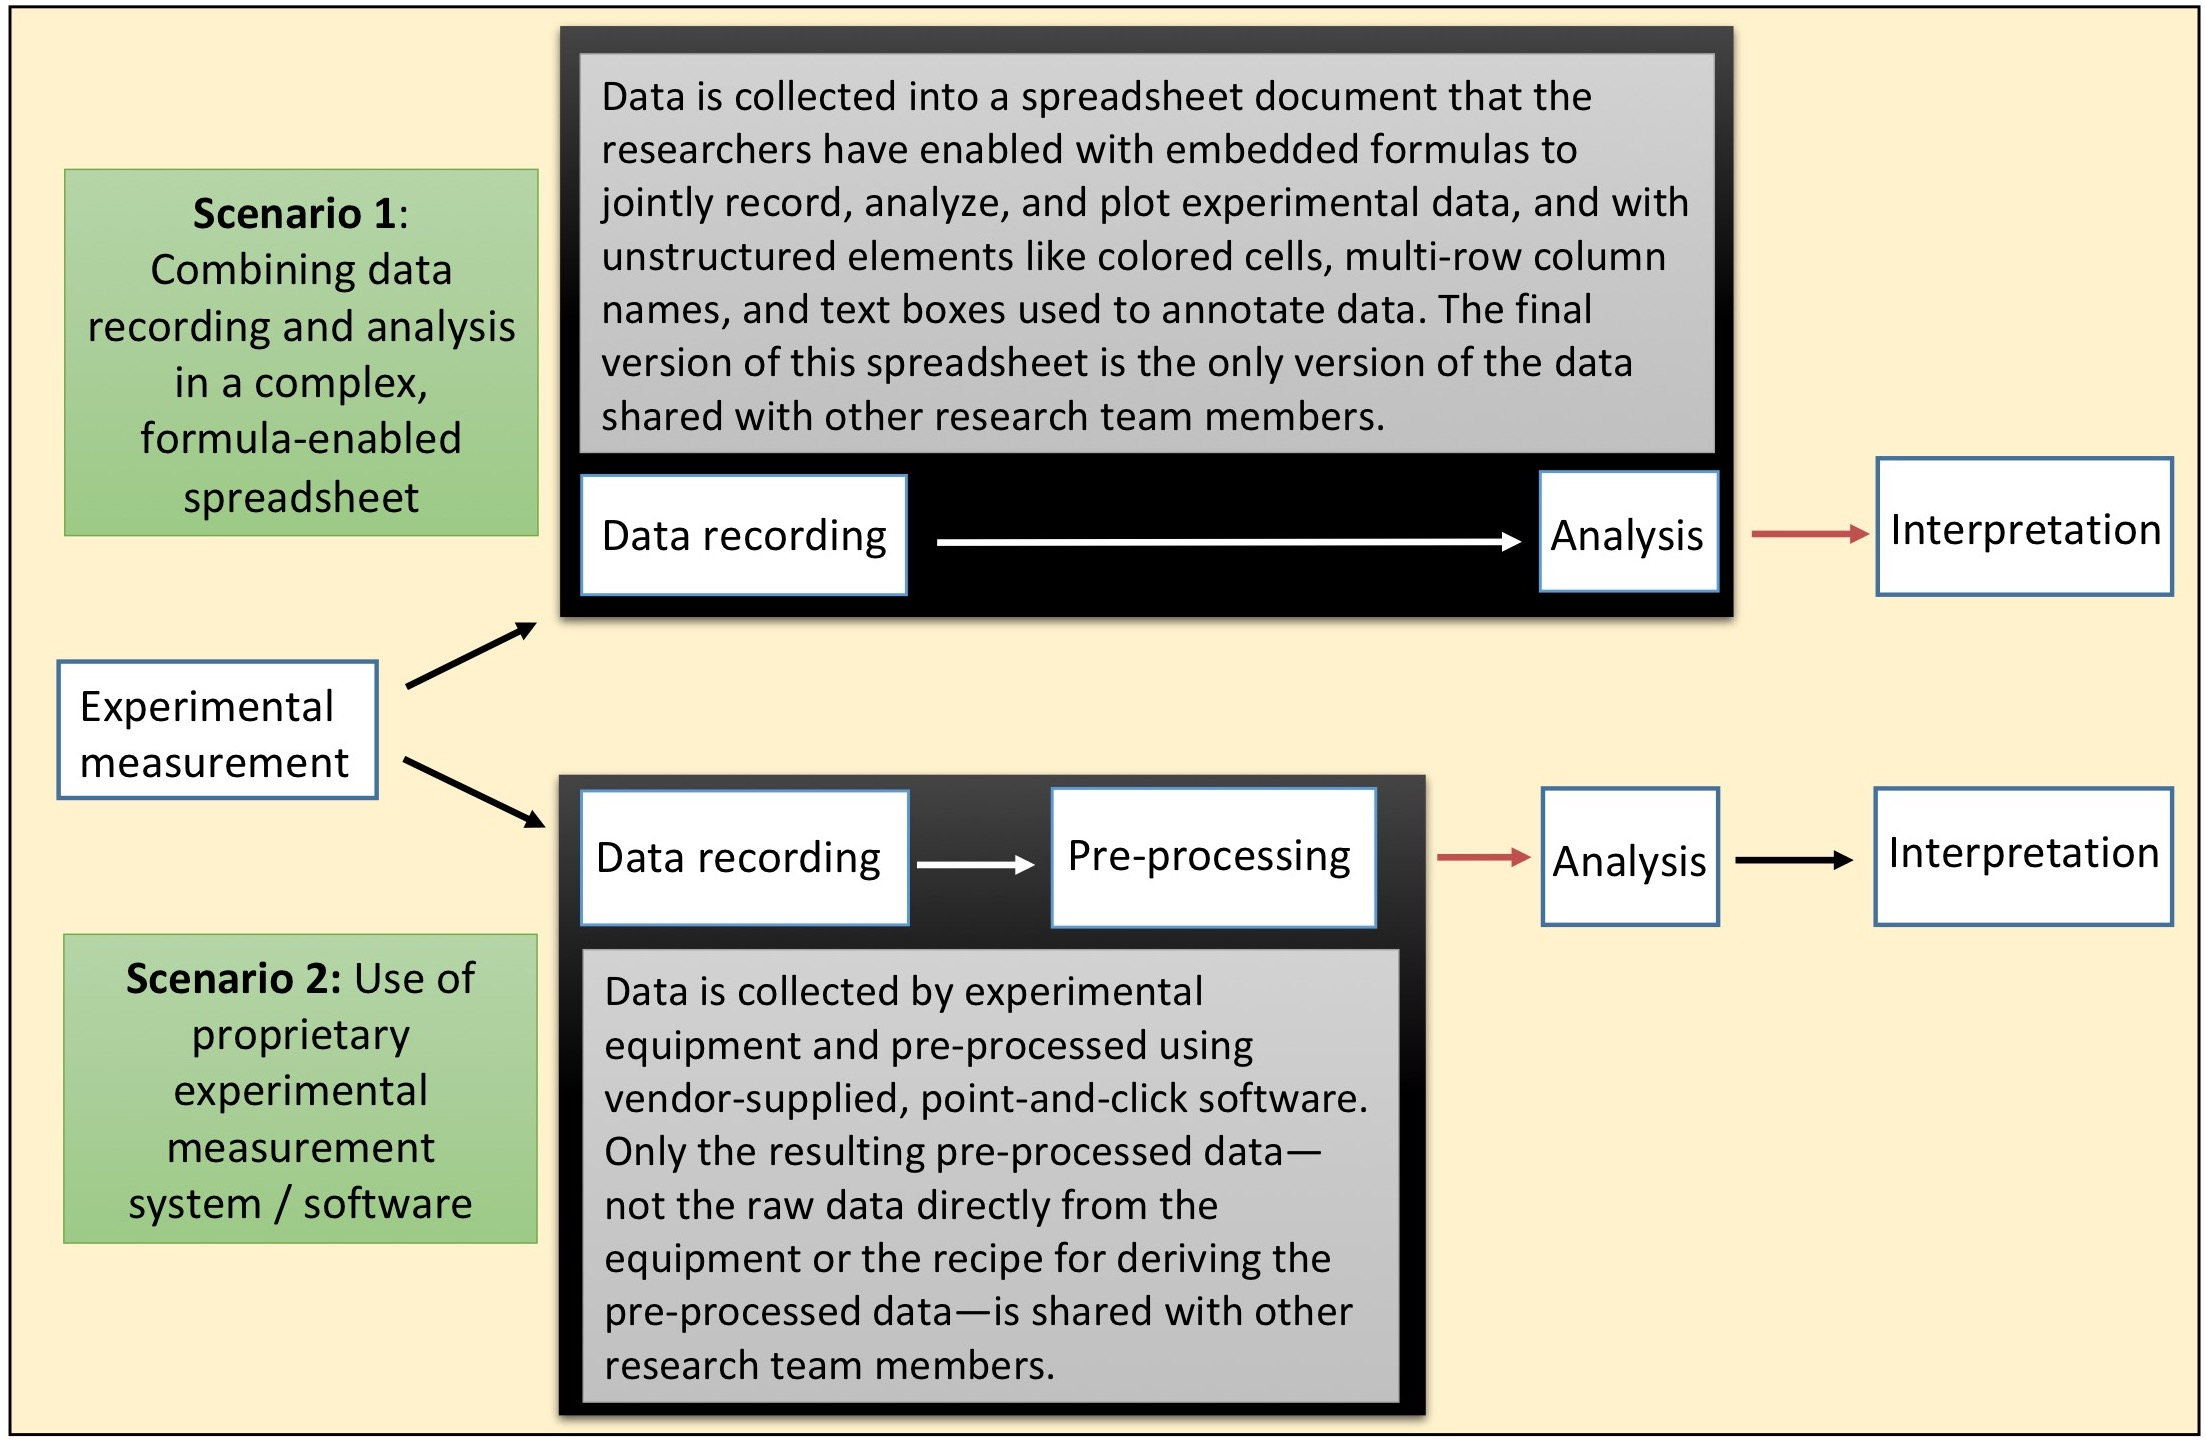
\includegraphics[width=\textwidth]{figures/existing_blackboxes} \caption[Two scenarios where 'black boxes' of non-transparent, non-reproducible data handling exist in research data workflows at the stages of data recording and pre-processing]{Two scenarios where 'black boxes' of non-transparent, non-reproducible data handling exist in research data workflows at the stages of data recording and pre-processing. These create potential points of failure for reproducible research. Red arrows indicate where data is passed to other research team members, including statisticians / data analysts, often within complex or unstructured spreadsheet files.}\label{fig:workflow}
\end{figure}

It is widely known and discussed among data scientists, mathematical modelers,
and statisticians \citep{broman2018data, krishnan2016towards} that there is
frequently a need to discard, transform, and reformat various elements of the
data shared with them by laboratory-based researchers, and that data is often
shared in an unstructured format, increasing the risks of introducing errors
through reformatting before applying more advanced computational methods.
Instead, a critical need for reproducibility is for the transparent and clear
sharing across research teams of: (1) raw data, directly from hand-recording or
directly output from experimental equipment; (2) data that has been
pre-processed as necessary (e.g., gating for flow cytometry data, feature
identification for metabolomics data), saved in a consistent, structured format,
and (3) a clear and repeatable description of how the pre-processed data was
generated from the raw data \citep{broman2018data, ellis2018share}.

To enhance data reproducibility, it is critical to create a clear separation
among data recording, data pre-processing, and data analysis---breaking up
commonly existing ``black boxes'' in data handling across the research process.
Such a rigorous demarcation requires some change in the conventional
understanding and use of spreadsheets and a recognition by biomedical
researchers that recent advances in computer programming languages, especially
the R programming language, provide user-friendly and accessible tools and
concepts that can be used to extend a transparent and reproducible data workflow
to the steps of data recording and pre-processing. Among our team, we have found
that there are many common existing practices---including use of spreadsheets
with embedded formulas that concurrently record and analyze experimental data,
problematic management of project files, and reliance on proprietary,
vendor-supplied point-and-click software for data pre-processing---that can
interfere with the transparency, reproducibility, and efficiency of
laboratory-based biomedical research projects, problems that have also been
identified by others as key barriers to research reproducibility
\citep{broman2018data, bryan2018excuse, ellis2018share, marwick2018packaging}. In
these training modules, we have choosen topics that tackle barriers to
reproducibility that have straightforward, easy-to-teach solutions, but which
are still very common in biomedical laboratory-based research programs.

\subsection{License}\label{license}

This book is licensed under the \href{https://creativecommons.org/licenses/by-nc-sa/4.0/}{Creative Commons
Attribution-NonCommercial-ShareAlike 4.0 International
License}, while all code in
the book is under the \href{https://opensource.org/licenses/MIT}{MIT license}.

\chapter{Experimental Data Recording}\label{experimental-data-recording}

This section includes modules on:

\begin{itemize}
\tightlist
\item
  \hyperref[module1]{Module 2.1: Separating data recording and analysis}
\item
  \hyperref[module2]{Module 2.2: Principles and power of structured data formats}
\item
  \hyperref[module3]{Module 2.3: The ``tidy'' data format}
\item
  \hyperref[module4]{Module 2.4: Designing templates for ``tidy'' data collection}
\item
  \hyperref[module5]{Module 2.5: Example: Creating a template for ``tidy'' data collection}
\item
  \hyperref[module6]{Module 2.6: Organizing project files}
\item
  \hyperref[module7]{Module 2.7: Creating project directory templates}
\item
  \hyperref[module8]{Module 2.8: Example: Creating a project template}
\item
  \hyperref[module9]{Module 2.9: Harnessing version control for transparent data recording}
\item
  \hyperref[module10]{Module 2.10: Enhance the reproducibility of collaborative research with version control platforms}
\item
  \hyperref[module11]{Module 2.11: Using Git and GitHub to implement version control}
\end{itemize}

\section{Separating data recording and analysis}\label{module1}

Do you use spreadsheets within your scientific work? If so, you're not alone. In
fact, studies have surveyed scientists about their work practices, and they've
found that spreadsheets are a common tool. Examples include surveys of over 250
biomedical researchers at the University of Washington \citep{anderson2007issues},
and of neuroscience researchers at the University of Newcastle. In both these
studies, most respondents reported that they used spreadsheets and other
general-purpose software in their research \citep{altarawneh2017pilot}. A working
group on bioinformatics and data-intensive science similarly found spreadsheets
were the most common tool used across attendees \citep{barga2011bioinformatics}.

These software tools, such as Microsoft Excel or Google Sheets, provide for
manual or automated entry of data into rows and columns of cells. Standard or
custom formulas and other operations can be applied to the cells, and are
commonly used to reformat or clean the data, calculate various statistics, and
to generate simple plots; all of which are embedded as additional data entries
and programming elements within the spreadsheet. While these tools greatly
improved the paper worksheets on which they were originally based
\citep{campbell2007number}, this all-in-one practice impedes the transparency and
reproducibility of both recording and analysis of the large and complex data
sets that are routinely generated in life science experiments.

To improve the computational reproducibility of a research project, it is
critical for biomedical researchers to learn the importance of maintaining
recorded experimental data as ``read-only'' files, separating data recording from
any data pre-processing or data analysis steps \citep{broman2018data, marwick2018packaging}.

In this module, we'll talk about why spreadsheets are so popular, as well
as some of their features that are beneficial for researchers. However, there
are also many problems they can introduce, particularly when spreadsheets are
used in a way that combines data collection with data pre-processing and analysis.
We'll walk through some of these problems, and in later modules we'll walk you
through alternatives, where spreadsheets are limited to recording data (if they're
used at all), while steps of pre-processing and analysis are done with other
tools.

\textbf{Objectives.} After this module, the trainee will be able to:

\begin{itemize}
\tightlist
\item
  Explain why spreadsheets are a popular tool among scientists
\item
  Explain the difference between data recording and data analysis
\item
  Understand why collecting data on spreadsheets with embedded formulas impedes
  reproducibility
\item
  Compare ways that spreadsheets can be used as a solid research tool
  versus other ways their use can be problematic
\item
  Discuss downsides to using spreadsheets for data analysis in scientific
  research
\end{itemize}

\subsection{Popularity of spreadsheets}\label{popularity-of-spreadsheets}

All of us authors are old enough to remember when home computers were a novelty.
When you first got a computer in your home, it opened up all kinds of new powers.

For one of us, one particularly exciting piece of software was something called
\emph{The Print Shop}. This software let you be an amateur graphic designer. You could
design things like signs and invitations. Because the printer paper at the time
was connected from one sheet to the next, with perforations between, you could
even make long banners. ``Happy Birthday'' banners, ``Congratulations'' banners,
``Welcome Home'' banners: you could do it all. For someone who'd never had these
tools before, it was thrilling.

This was evidently how early spreadsheet software made business executives feel.
Before these programs, if an executive wanted to crunch some numbers, they'd
have to send a request to their accounting department. The initial spreadsheet
program (VisiCalc) disrupted this process. It allowed one person to quickly
apply and test different models or calculations on recorded data
\citep{levy1984spreadsheet}. These spreadsheet programs allowed non-programmers to
engage with data, including data processing and analysis tasks, in a way that
previously required programming expertise \citep{levy1984spreadsheet}. With
spreadsheet programs an executive could just play with the numbers themselves.

Because an early target for spreadsheet programs was these business
executives, the programs were designed to be very simple and easy to use---just
one step up in complexity from crunching numbers on the back of an envelope
\citep{campbell2007number}.Spreadsheet programs in fact became so popular within
businesses that many attribute these programs with driving the uptake of
personal computers \citep{campbell2007number}.

Spreadsheets have become so popular in part because so many people know how to
use them, at least in basic ways, and so many people have the software on their
computers that files can be shared with almost a guarantee that everyone will be
able to open the file on their own computer \citep{hermans2016spreadsheets}.
Spreadsheets use the visual metaphore of a traditional gridded ledger sheet
\citep{levy1984spreadsheet}, providing an interface that is easy for users to
immediately understand and for which they can easily create a mental map
\citep{birch2018future, barga2011bioinformatics}. This visually clear interface also means that
spreadsheets can be printed or incorporated into other documents ``as-is'', as a
workable and understandable table of data values. In fact, some of the most
popular plug-in software packages for the early spreadsheet program Lotus 1-2-3
were programs for printing and publishing spreadsheets \citep{campbell2007number}.
This ``What You See Is What You Get'' interface was a huge advance from previous
methods of data analysis for the first spreadsheet program, VisiCalc, providing
a ``window to the data'' that was accessible to business executives and others
without programming expertise \citep{creeth1985microcomputer}. Several surveys of
researchers have found that spreadsheets were popular because of their
simplicity and ease-of-use \citep{anderson2007issues, altarawneh2017pilot, barga2011bioinformatics}. By contrast, databases and scripted programming
languages can be perceived as requiring a cognitive load and lengthy training
that is not worth the investment when an easier tool is available
\citep{hermans2016spreadsheets, anderson2007issues, myneni2010organization, barga2011bioinformatics, topaloglou2004biological}.

Software tools like The Print Shop and spreadsheet programs were perfectly
designed for amateurs to begin to do some of the things that otherwise required
outsourcing to a professional. They are fantastic tools for amateur exploration.
They make it fun to test out ideas.

However, these types of software tools are so easy and convenient to use that it
can be tempting to let them replace more solid, production-level tools. It's
easy, in other words, to make them the \emph{only} tool used to tackle a problem,
rather than just the \emph{first} tool to use to explore a solution. These tools are
also often the cheapest option, either in monetary cost or in the time
investment to learn them. However, they often fail when they're used as a
replacement for more solid options. This can be the case with spreadsheet
programs in biomedical research, where spreadsheets are often used not only as a
straightforward way to record data (for which they can be a very solid tool),
but also to develop complex pipelines that process and analyze the data once its
been collected.

\subsection{Hazards of combining recording and analysis}\label{hazards-of-combining-recording-and-analysis}

In some cases, researchers use spreadsheets solely to record data, as a simple
type of database \citep{birch2018future}. However, biomedical researchers often use
spreadsheets to both record and analyze experimental data \citep{anderson2007issues, broman2018data}. In this case, data processing and analysis is implemented
through the use of formulas and macros embedded within the spreadsheet.

When a spreadsheet has formulas or macros within it, the spreadsheet program
creates an internal record of how cells are connected through these formulas.
For example, say the value in a specific cell is converted from Fahrenheit to
Celsius to fill a second cell, and then that value is combined with other values
in a column to calculate the mean temperature across several observations. In
this case, the spreadsheet program has internally saved how the later cells
depend on the earlier ones. When you change the value recorded in a cell of a
spreadsheet, the spreadsheet program queries this record and only recalculates
the cells that depend on that cell. This process allows the program to quickly
``react'' to any change in cell inputs, immediately providing an update to all
downstream calculations and analyses \citep{levy1984spreadsheet}. Since early in
their development, spreadsheet programs have also included \emph{macros}, ``a single
computer instruction that stands for a sequence of operations''
\citep{creeth1985microcomputer}.

There are some important downsides to using these tools within scientific
research to create spreadsheets that combine data recording with data analysis.
Those include:

\begin{itemize}
\tightlist
\item
  Raw data are often lost
\item
  Analysis steps are often opaque
\item
  There is a higher potential for errors in the analysis
\item
  There are better software tools available for data analysis
\item
  It will make it more difficult to collaborate with statisticians
\end{itemize}

Let's take a look at each of these.

\textbf{Raw data often lost}

One of the key tenets of ensuring that research is computationally reproducible
is to always keep a copy of all raw data, as well as the steps taken to get from
the raw data to a cleaned version of the data through to the results of data
analysis. However, maintaining an easily accessible copy of all original raw data
for a project is a common problem among biomedical researchers
\citep{goodman2014ten}, especially as team members move on from a laboratory group
\citep{myneni2010organization}. In fact, one study of
operational spreadsheets found:

\begin{quote}
``The data used in most spreadsheets is undocumented and there is no practical
way to check it. Even the original developer would have difficulty checking the
data.'' \citep{powell2009errors}
\end{quote}

One thing that can contribute to this problem is the use of spreadsheets to
jointly record and analyze data. First, data in a spreadsheet is typically not
saved as ``read-only'', so it is possible for it to be accidentally overwritten:
in situations where spreadsheets are shared among multiple users, original cell
values can easily be accidentally written over, and it may not be clear who last
changed a value, when it was changed, or why \citep{altarawneh2017pilot}. Further,
raw and processed data are combined in a spreadsheet, which makes it hard to
identify which data points within the spreadsheet make up the raw data and which
are the result of processing that raw data.

Another issue is that many spreadsheets use a proprietary format. In the
development of spreadsheet programs, this use of proprietary binary file formats
helped a software program keep users, increasing barriers for a user to switch
to a new program (since the new program wouldn't be able to read their old
files) \citep{campbell2007number}. However, this file format may be hard to open in
the future, as software changes and evolves \citep{michener2015ten}; by comparison,
plain text files should be widely accessible through general purpose tools---a
text editor is a type of software available on all computers, for
example---regardless of changes to proprietary software like Microsoft Excel.

\textbf{Analysis steps are often opaque}

To keep analysis steps clear---whether the calculation is being done in scripted
code or in spreadsheets or in pen-and-paper calculations---it is important to
document what is being done at each step and why \citep{goodman2014ten}. Scripted
languages allow for code comments, which are written directly into the script
but not evaluated by the computer, and so can be used to document steps within
the code without changing the operation of the code. Further, the program file
itself often presents a linear, step-by-step view of the pipeline, stored
separated from the data \citep{creeth1985microcomputer}. Calculations done
with pen-and-paper (e.g., in a laboratory notebook) can be annotated with text
to document the steps. Spreadsheets, on the other hand, are often poorly
documented, or documented in ways that are hard to keep track of.

Within spreadsheets, the logic and methods behind the pipeline of data
processing and analysis is often not documented, or only documented with cell
comments (hard to see as a whole) or in emails, not the spreadsheet file.
One study that investigated a large collection of spreadsheets found that most
do not include documentation explaining the logic or implementation of data
processing and analysis implemented within the spreadsheet
\citep{hermans2016spreadsheets}. A survey of neuroscience researchers at a UK
institute found that about a third of respondents included no documentation
for spreadsheets used in their research laboratories \citep{altarawneh2017pilot}.

When spreadsheet pipelines are documented, it is often through methods that are
hard to find and interpret later. One study of scientific researchers found
that, when research spreadsheets were documented, it was often through ``cell
comments'' added to specific cells in the spreadsheet, which can be hard to
interpret inclusively to understand the flow and logic of a spreadsheet as a
whole \citep{altarawneh2017pilot}.

In some cases, teams use email chains, rather than the document itself, to
discuss and document functionality and changes in spreadsheets. They pass
versions of the spreadsheet file as attachments of emails discuss the
spreadsheet in the email body.

One research team investigated over 700,000 emails from employees of Enron that
were released during legal proceedings \citep{hermans2015enron}. They specifically
investigated the spreadsheets attached to these emails (over 15,000
spreadsheets) and how teams discussed the spreadsheets within the emails
themselves . They found that the logic and methods of calculations within the
spreadsheets were often documented within the bodies of emails. This means that,
if someone needs to figure out why a step was taken or identify when an error
was introduced into a spreadsheet, they must dig through the chain of old emails
documenting that spreadsheet, rather than having the relevant documentation
within the spreadsheet's own file.

Adding to this issue is that data processing and analysis pipelines for
spreadsheets are not carefully designed; instead, it's more typically for
spreadsheet user to start by directly entering data and formulas without a clear
overall plan \citep{altarawneh2017pilot}. As a result, research spreadsheets are
often not designed to follow a common structure for the research field or for
the laboratory group \citep{anderson2007issues}.

Another problem comes up because there may only be one person on the team who
fully understands the spreadsheet: the person who created the spreadsheet
\citep{myneni2010organization}. This is particularly common if the spreadsheet
includes complex macros or a complicated structure in the analysis pipeline
\citep{creeth1985microcomputer}. This practice creates a heavy dependence on the
person who created that spreadsheet anytime the data or results in that
spreadsheet need to be interpreted. This is particularly problematic in projects
where the spreadsheet will be shared for collaboration or adapted to be used in
a future project, as is often done in scientific research groups. In this case,
it can be hard to ``onboard'' new people to use the file, and much of the work and
knowledge about the spreadsheet can be lost when that person moves on from the
business or laboratory group \citep{creeth1985microcomputer, myneni2010organization}.

If you share a spreadsheet with numerous and complex macros and formulas
included to clean and analyze the data, it can take an extensive amount of time,
and in some cases may be impossible, for the researcher you share it with to
decipher what is being done to get from the original data input in some cells to
the final results shown in others and in graphs. Further, if others can't figure
out the steps being done through macros and formulas in a spreadsheet, they will
not be able to check it for problems in the logic of the overall analysis
pipeline or for errors in the specific formulas used within that pipeline. They
also will struggle to extend and adapt the spreadsheet to be used for other
projects. These problems come up not only when sharing with a collaborator, but
also when reviewing spreadsheets that you have previously created and used (as
many have noted, your most frequent collaborator will likely be ``future you'').
In fact, one survey of biomedical researchers at the University of Washington
noted that,

\begin{quote}
``The profusion of individually created spreadsheets containing overlapping and
inconsistently updated data created a great deal of confusion within some labs.
There was little consideration to future data exchange of submission
requirements at the time of publication.''
\citep{anderson2007issues}
\end{quote}

\textbf{Potential for errors}

Because spreadsheets often do a poor job of making the analysis steps
transparent, they can be prone to bugs in analysis. As one early article on
the history of spreadsheet programs notes:

\begin{quote}
``People tend to forget that even the most elegantly crafted spreadsheet is a
house of cards, ready to collapse at the first erroneous assumption. The
spreadsheet that looks good but turns out to be tragically wrong is becoming
a familiar phenomenon.'' \citep{levy1984spreadsheet}
\end{quote}

Indeed, previous studies have found that errors are very common within
spreadsheets \citep{hermans2016spreadsheets}. For example, one study of 50
operational spreadsheets found that about 90\% contained at least one error
\citep{powell2009errors}.

In part, it is easier to make errors in spreadsheets and harder to catch errors
in later work with a spreadsheet because the formulas and connections between
cells aren't visible when you look at the spreadsheet---they're behind the
scenes \citep{birch2018future}. This makes it hard to get a clear and complete
view of the pipeline of analytic steps in data processing and analysis within a
spreadsheet, or to discern how cells are connected within and across sheets of
the spreadsheet.

Some characteristics of spreadsheets may heighten chances for errors. These
include high conditional complexity, which can result from lots of branching of
data flow through if / else structures, as well as formulas that depend on a
large number of cells or that incorporate many functions
\citep{hermans2016spreadsheets}. Following the logical chain of spreadsheet formulas
can be particularly difficult when several calculations are chained in a row
\citep{hermans2015enron}. In some cases, if you are trying to figure out very long
chains of dependent formulas across spreadsheet cells, you may even have to
sketch out by hand the flow of information through the spreadsheet to understand
what's going on \citep{nardi1990spreadsheet}. When a spreadsheet uses macros, it can
also make it particularly hard to figure out the steps of an analysis and to
diagnose and fix any bugs in those steps \citep{nash2006spreadsheets, creeth1985microcomputer}. One study investigated how spreadsheets are used in
practice and noted that, ``Many spreadsheets are so chaotically designed that
auditing (especially of a few formulas) is extremely difficult or impossible.''
\citep{powell2009errors}

In some cases, formula dependencies might span across different sheets of a
spreadsheet file. These cross-sheet dependencies can make the analysis steps
even more opaque \citep{hermans2016spreadsheets}, as a change in the cell value of
one sheet might not be immediately visible as a change in another cell on that
sheet (the same is true for spreadsheets so large that all the cells in a sheet
are not concurrently visible on the screen). Other common sources of errors
included incorrect references to cells inside formulas and incorrect use of
formulas \citep{powell2009errors} or errors introduced through the common practice of
copying and pasting when developing spreadsheets \citep{hermans2016spreadsheets}.

There are methods that have been brought from more traditional programming work
into spreadsheet programming to try to help limit errors, including a tool
called \emph{assertions} that allows users to validate data or test logic within their
spreadsheets \citep{hermans2016spreadsheets}. However, these are often not
implemented, in part perhaps because many spreadsheet users see themselves as
``end-users'', creating spreadsheets for their own personal use rather than as
something robust to future use by others, and so don't seek out strategies
adopted by programmers when creating stable tools for others to use
\citep{hermans2016spreadsheets}. In practice, though, a spreadsheet is often used
much longer, and by more people, than originally intended. From early in the
history of spreadsheet programs, users have shared spreadsheet files with
interesting functionality with other users \citep{levy1984spreadsheet}, and the
lifespan of a spreadsheet can extend and extend---a spreadsheet created by one
user for their own personal use can end up being used and modified by that
person or others for years \citep{hermans2016spreadsheets}.

\textbf{Better software tools are available}

While spreadsheets serve as a widely-used tool for data recording and analysis,
in many cases spreadsheets programs are poorly suited to pre-process and analyze
scientific data compared to other programs. As tools and interfaces continue to
develop that make other software more user-friendly to those new to programming,
scientists may want to reevaluate the costs and benefits, in terms of both time
required for training and aptness of tools, of spreadsheet programs compared to
scripted programming languages like R and Python.

Several problems have been identified with spreadsheet programs in the context
of recording and, especially, analyzing scientific data. First, some statistical
methods may be inferior to those available in other statistical programming
language. Many statistical operations require computations that cannot be
perfectly achieved with a computer, since the computer must ultimately solve
many mathematical problems using numerical approximations (e.g., calculus). The
choice of the algorithms used for these approximations heavily influence how
closely a result approximates the true answer. Since the most popular
spreadsheet program (Excel) is closed-source, it is hard to identify and
diagnose such problems, and there is likely less of an incentive for problems in
statistical methodology to be fixed (rather than using development time and
funds to increase easier-to-see functionality in the program).

A series of papers examined the quality of statistical methods in several
statistical software programs, including Excel, starting in the 1990s
\citep{mccullough1999accuracy, mccullough1999assessing, mccullough2002accuracy, mccullough2005accuracy, mccullough2008accuracy, melard2014accuracy}. In the
earliest studies, they found some concerns across all programs considered
\citep{mccullough1999accuracy, mccullough1999assessing}. One of the biggest
concerns, however, was that there was little evidence over the years that the
identified problems in Excel were resolved, or at least improved, over time
\citep{mccullough2001does, mccullough2008accuracy}. The authors note that there may
be little incentive for checking and fixing problems with algorithms for
statistical approximation in closed-source software like Excel, where sales
might depend more on the more immediately evident functionality in the software,
while problems with statistical algorithms might be less evident to potential
users \citep{mccullough2001does}.

Open-source software, on the other hand, offers pathways for identifying and fixing
any problems in the software, including for statistical algorithms and methods
implemented in the software's code. Since the full source code is available, researchers
can closely inspect the algorithms being used and compare them to the latest
knowledge in statistical computing methodology. Further, if an inferior algorithm is in
use, most open-source software licenses allow a user to adapt and extend the software,
including to implement better statistical algorithms.

Another problem is that spreadsheet programs can include automated functionality
that's meant to make something easier for most users, but that might invisibly
create some problems. A critical problem, for example, has been identified when
using Excel for genomics data. When Excel encounters a cell value in a format
that seems like it could be a date (e.g., ``Mar-3-06''), it will try to convert
that cell to a ``date'' class. Many software programs save date as this special
``date'' format, where it is printed and visually appears in a format like
``3-Mar-06'' but is saved internally by the program as a number (for Microsoft
Excel, the number of days since January 1, 1900 \citep{willekens2013chronological}).
By doing this, the software can more easily undertake calculations with dates,
like calculating the number of days between two dates or which of two dates is
earlier. Bioinformatics researchers at the National Institutes of Health found
that Excel was doing this type of automatic and irreversible date conversion for
30 gene names, including ``MAR3'' and ``APR-4'', resulting in these gene names being
lost for further analysis \citep{zeeberg2004mistaken}.

Avoiding this automatic date conversion required specifying that columns
susceptible to these problems, including columns of gene names, should
be retained in a ``text'' class in Excel's file import process. While this
problem was originally identified and published in 2004 \citep{zeeberg2004mistaken},
along with tips to identify and avoid the problem, a study in 2016 found that
approximately a fifth of genomics papers investigated in a large-scale review
had gene name errors resulting from Excel automatic conversion, with the rate of
errors actually increasing over time \citep{ziemann2016gene}.

Other automatic conversion problems caused the lost of clone identifiers that
were composed of digits and the letter ``E'' \citep{zeeberg2004mistaken, welsh2017escape}. These were assumed to be expressing a number using scientific
notation and so automatically and irreversibly converted to a numeric class.
Further automatic conversion problems can be caused by cells that start with an
operator (e.g., ``+ control'') or with leading zeros in a numeric identifier
(e.g., ``007'') \citep{welsh2017escape}.

Finally, spreadsheet programs can be limited as analysis needs become more
complex or large \citep{topaloglou2004biological}. For example, spreadsheets can be
problematic when integrating or merging large, separate datasets
\citep{birch2018future}. Further, while spreadsheet programs continue to expand in
their capacity for data, for very large datasets they continue to face limits
that may be reached in practical applications \citep{birch2018future}---until
recently, for example, Excel could not handle more than one million rows of data
per spreadsheet. Even when spreadsheets can handle larger data, their efficiency
in running data processing and analysis pipelines across large datasets can be
slow compared to code implemented with other programming languages.

\textbf{Difficulty collaborating with statisticians}

Modern biomedical researchers requires large teams, with statisticians and
bioinformaticians often included, to enable sophisticated processing and
analysis of experimental data. However, the process of combining data recording
and analysis, especially through the use of spreadsheet programs, can create
barriers in working across disciplines. One group defined these issues as ``data
friction'' and ``science friction''---the extra steps and work required at each
interface where data passes, for example, from a machine to analysis or from a
collaborator in one discipline to one in a separate discipline
\citep{edwards2011science}.

When collaborating with statisticians or bioinformaticians, one of the key
sources of this ``data friction'' can result from the use of spreadsheets to
jointly record and analyze experiemental data. First, spreadsheets are easy to
print or copy into another format (e.g., PowerPoint presentation, Word
document), and so researchers often design spreadsheets to be immediately
visually appealing to viewers. For example, a spreadsheet might be designed to
include hierarchically organized headers (e.g., heading and subheading, some
within a cell merged across several columns), or to show the result of a
calculation at the bottom of a column of observations (e.g., ``Total'' in the last
cell of the column) \citep{teixeira2016emergence}. Multiple separate small tables
might be included in the same sheet, with empty cells used for visual
separation, or use a ``horizontal single entry'' design , where the headers are in
the leftmost column rather than the top row \citep{teixeira2016emergence}.

These spreadsheet design choices make it much more difficult for the contents of
the spreadsheet to be read into other statistical programs. These types of data
require several extra steps in coding, in some cases fairly complex coding, with
regular expressions or logical rules needed to parse out the data and convert it
to the needed shape, before the statistical work can be done for the dataset.
This is a poor use of time for a collaborating statistician, especially if it
can be avoided through the design of the data recording template. Further, it
introduces many more chances for errors in cleaning the data.

Further, information embedded in formulas, macros, and extra formatting like
color or text boxes is lost when the spreadsheet file is input into other
programs. Spreadsheets allow users to use highlighting to represent information
(e.g., measurements for control animals shown in red, those for experiment
animals in blue) and to include information or documentation in text boxes. For
example, one survey study of biomedical researchers at the University of
Washington included this quote from a respondent: ``I have one spreadsheet that
has all of my chromosomes \ldots{} and then I've gone through and color coded it for
homozygosity and linkage.'' \citep{anderson2007issues} All the information encoded in
this sheet through color will be lost when the data from the spreadsheet is read
into another statistical program.

\subsection{Approaches to separate recording and analysis}\label{approaches-to-separate-recording-and-analysis}

In the remaining modules in this section, we will present and describe
techniques that can be used to limit or remove these problems. First, in the
next few modules, we will walk through techniques to design data recording
formats so that data is saved in a consistent format across experiments within a
laboratory group, and in a way that removes ``data friction'' for collaboration
with statisticians or later use in scripted code. These techniques can be
immediately used to design a better spreadsheet to be used solely for data
collection.

In later modules, we will discuss the use of project directories to coordinate
data recording and analysis steps within a directory, while using separate files
for data recording versus data processing and analysis. These more advanced
formats will enable the use of quality assurance / control measures like testing
of data entry and analysis functionality, better documentation of data analysis
pipelines, and easy use of version control to track projects and collaborate
transparently and with a recorded history.

\section{Principles and power of structured data formats}\label{module2}

Guru Madhavan, Senior Director of Programs at the National Academy of
Engineering, wrote a book in 2015 called \emph{Applied Minds: How Engineers Think}.
In this book, he described a powerful tool for engineers---standards:

\begin{quote}
``Standards are for products what grammar is for language. People sometimes
criticize standards for making life a matter of routine rather than inspiration.
Some argue that standards hinder creativity and keep us slaves to the past.
But try imagining a world without standards. From tenderloin beef cuts to
the geometric design of highways, standards may diminish variety and
authenticity, but they improve efficiency. From street signs to nutrition
labels, standards provide a common language of reason. From Internet
protocols to MP3 audio formats, standards enable systems to work together.
From paper sizes \ldots{} to George Laurer's Universal Product Code, standards
offer the convenience of comparability.'' \citep{madhavan2015applied}
\end{quote}

Standards can be a powerful tool for biomedical researchers, as well, including
when it comes to recording data.
The format in which experimental data is recorded can have a large influence on
how easy and likely it is to implement reproducibility tools in later stages of
the research workflow. Recording data in a ``structured'' format brings many
benefits. In this module, we will explain what makes a dataset ``structured'' and
why this format is a powerful tool for reproducible research.

Every extra step of data cleaning is another chance to introduce errors in
experimental biomedical data, and yet laboratory-based researchers often share
experimental data with collaborators in a format that requires extensive
additional cleaning before it can be input into data analysis \citep{broman2018data}.
Recording data in a ``structured'' format brings many benefits for later stages of
the research process, especially in terms of improving reproducibility and
reducing the probability of errors in analysis \citep{ellis2018share}. Data that is
in a structured, tabular, two-dimensional format is substantially easier for
collaborators to understand and work with, without additional data formatting
\citep{broman2018data}. Further, by using a consistent structured format across many
or all data in a research project, it becomes much easier to create solid,
well-tested code scripts for data pre-processing and analysis and to apply those
scripts consistently and reproducibly across datasets from multiple experiments
\citep{broman2018data}. However, many biomedical researchers are unaware of this
simple yet powerful strategy in data recording and how it can improve the
efficiency and effectiveness of collaborations \citep{ellis2018share}. In this
module, we'll walk through several types of standards that can be used when
recording biomedical data.

\textbf{Objectives.} After this module, the trainee will be able to:

\begin{itemize}
\tightlist
\item
  Define ontology, minimum information, and file format
\item
  List the elements of a structured data format
\item
  Explain how standards can improve scientific data recording
\item
  Find existing ontologies for biological and biomedical research
\end{itemize}

\subsection{Data recording standards}\label{data-recording-standards}

Many people and organizations (including funders) are excited about the idea of
developing and using data standards. Good standards---ones that are widely
adapted by researchers---can help in making sure that data submitted to data
repositories are used widely and that software can be developed that is
interoperable with data from many research groups.

For a simple example, think about recording dates. The minimum
information standard for a date might always be the same---a recorded value
must include the day of the month, month, and year. However, this information
can be structured in a variety of ways. Often in scientific data, it's common
to record this information going from the largest to smallest units, so March
12, 2006, would be recorded ``2006-03-12''. Another convention (especially in the
US) is to record the month first (e.g., ``3/12/06''), while another (more common
in Europe) is to record the day of the month first (e.g., ``12/3/06'').

If you are trying to combine data from different datasets with dates, and all
use a different structure, it's easy to see how mistakes could be introduced
unless the data is very carefully reformatted. For example, March 12 (``3-12''
with month-first, ``12-3'' with day-first) could be easily mistaken to be December
3, and vice versa. Even if errors are avoided, combining data in different
structures will take more time than combining data in the same structure,
because of the extra needs for reformatting to get all data in a common
structure.

Standards can operate both at the level of individual research groups and at the
level of the scientific community as a whole. The potential advantages of
community-level standards are big: they offer the chance to develop
common-purpose tools and code scripts for data analysis, as well as make it
easier to re-use and combine experimental data from previous research that is
posted in open data repositories. If a software tool can be reused, then more
time can be spent in developing and testing it, and as more people use it, bugs
and shortcomings can be identified and corrected. Community-wide standards can
lead to databases with data from different experiments, and from different
laboratory groups, structured in a way that makes it easy for other researchers
to understand each dataset, find pieces of data of interest within datasets, and
integrate different datasets \citep{lynch2008big}. Similarly, with community-wide
standards, it can become much easier for different research groups to
collaborate with each other or for a research group to use data generated by
equipment from different manufacturers \citep{schadt2010computational}. As
an article on interoperable bioscience data notes,

\begin{quote}
``Without community-level harmonization and interoperability, many community
projects risk becoming data silos.'' \citep{sansone2012toward}
\end{quote}

However, there are important limitations to community-wide standards, as well.
It can be very difficult to impose such standards top-down and community-wide,
particularly for low-throughput data collection (e.g., laboratory bench
measurements), where research groups have long been in the habit of recording
data in spreadsheets in a format defined by individual researchers or research
groups. One paper highlights this point:

\begin{quote}
``The data exchange formats PSI-MI and MAGE-ML have helped to get many of the
high-throughput data sets into the public domain. Nevertheless, from a bench
biologist's point of view benefits from adopting standards are not yet
overwhelming. Most standardization efforts are still mainly an investment for
biologists.'' \citep{brazma2006standards}
\end{quote}

Further, in some fields, community-wide standards have struggled to remain
stable, which can frustrate community members, as scripts and software must be
revamped to handle shifting formats \citep{buffalo2015bioinformatics, barga2011bioinformatics}. In some cases, a useful compromise is to follow a
general data recording format, rather than one that is very prescriptive. For
example, committing to recording data in a format that is ``tidy'' (which we
discuss extensively in the next module) may be much more flexible---and able to
meet the needs of a large range of experimental designs---than the use of a
common spreadsheet template or a more prescriptive standardized data format.

\subsection{Elements of a data recording standard}\label{elements-of-a-data-recording-standard}

Standards can clarify several elements: the vocabulary used within data, the
content that should be included in a dataset, and the format in which that
content is stored. One article names these three facets of a data standard as
\emph{ontologies}, \emph{minimum information}, and \emph{file formats} \citep{ghosh2011software}.

\textbf{Ontology standards.}

The first facet of a data standard is called an \emph{ontology} (sometimes called a
\emph{terminology} \citep{sansone2012toward}). An ontology helps define a vocabulary that
is controlled and consistent. It helps researchers, when they want to talk about
an idea or thing, to use one word, and just one word, and to ensure that it will
be the same word used by other researchers when they refer to that idea or
thing. Ontologies also help to define the relationships between ideas or
concrete things in a research area \citep{ghosh2011software}, but here we'll focus on
their use in provided a consistent vocabulary to use when recording data.

Let's start with a very simple example to give you an idea of what an ontology
is. What do you call a small mammal that is often kept as a pet and that has
four legs and whiskers and purrs? If you are recording data that includes this
animal, do you record this as ``cat'' or ``feline'' or maybe, depending on the
animal, even ``tabby'' or ``tom'' or ``kitten''? Similarly, do you record tuberculosis
as ``tuberculosis'' or ``TB'' or maybe even ``consumption''? If you do not use the
same word consistently in a dataset to record an idea, then while a human might
be able to understand that two words should be considered equivalent, a computer
will not be able to immediately tell.

At a larger scale, if a research community can adapt an ontology---one they
agree to use throughout their studies---it will make it easier to understand and
integrate datasets produced by different research laboratories. If every
research group uses the term ``cat'' in the example above, then code can easily be
written to extract and combine all data recorded for cats across a large
repository of experimental data. On the other hand, if different terms are used,
then it might be necessary to first create a list of all terms used in datasets
in the respository, then pick through that list to find any terms that are
exchangeable with ``cat'', then write script to pull data with any of those terms.

Several onotologies already exist or are being created for biological and other
biomedical research \citep{ghosh2011software}. For biomedical science, practice, and
research, the BioPortal website (\url{http://bioportal.bioontology.org/}) provides
access to over 1,000 ontologies, including several versions of the International
Classification of Diseases, the Medical Subject Headings (MESH), the National
Cancer Institute Thesaurus, the Orphanet Rare Disease Ontology and the National
Center for Biotechnology Information (NCBI) Organismal Classification. For each
ontology in the BioPortal website, the website provides a link for downloading
the ontology in several formats.

Try downloading one of the ontologies using a plaintext file format (the ``CSV''
choice in the download options at the BioPortal link). Once you do, you can open
it in your favorite spreadsheet program and explore how it defines specific
terms to use for each idea or thing you might need to discuss within that topic
area, as well as synonyms for some of the terms.

To use an ontology when recording your own data, just make sure you use the
ontology's suggested terms in your data. For example, if you'd like to use the
Ontology for Biomedical Investigations
(\url{http://bioportal.bioontology.org/ontologies/OBI}) and you are recording how many
children a woman has had who were born alive, you should name that column of the
data ``number of live births'', not ``\# live births'' or ``live births (N)'' or
anything else. Other collections of ontologies exist for fields of scientific
research, including the Open Biological and Biomedical Ontology (OBO) Foundry
(\url{http://www.obofoundry.org/}).

If there are community-wide ontologies in your field, it is worthwhile to use
them in recording experimental data in your research group. Even better is to
not only consistently use the defined terms, but also to follow any conventions
with capitalization. While most statistical programs provide tools to change
capitalization (for example, to change all letters in a character string to
lower case), this process does require an extra step of data cleaning and an
extra chance for confusion or for errors to be introduced into data.

\textbf{Minimum information standards}

Another part of a data standard is \emph{minimum information}. Within a data
recording standard, minimum information (sometimes also called \emph{minimum
reporting guidelines} \citep{sansone2012toward} or \emph{reporting requirements}
\citep{brazma2006standards}) specify what should be included in a dataset
\citep{ghosh2011software}. Using minimum information standards help ensure that data
within a laboratory, or data posted to a repository, contain a number of
required elements. This makes it easier to re-use the data, either to compare it
to data that a lab has newly generated, or to combine several posted datasets to
aggregate them for a new, integrated analysis, considerations that are growing
in importance with the increasing prevalence of research repositories and
research consortia in many fields of biomedical science \citep{keller2017evolution}.

One article that discusses software for systems biology provides a definition
as well as examples of minimum information within this field:

\begin{quote}
``Minimum information is a checklist of required supporting information for
datasets from different experiments. Examples include: Minimum Information About
a Microarray Experiment (MIAME), Minimum Information About a Proteomic
Experiment (MIAPE), and the Minimum Information for Biological and Biomedical
Investigations (MIBBI) project.'' \citep{ghosh2011software}
\end{quote}

\textbf{Standardized file formats}

While using a standard ontology and a standard for minimum information is a
helpful start, it just means that each dataset has the required elements
\emph{somewhere}, and using a consistent vocabulary---it doesn't specify where those
elements are in the data or that they'll be in the same place in every dataset
that meets those standards. As a result, datasets that all meet a common
standard can still be very hard to combine, or to create common data analysis
scripts and tools for, since each dataset will require a different process to
pull out a given element.

Computer files serve as a way to organize data, whether that's recorded
datapoints or written documents or computer programs \citep{kernighan1984unix}. A
\emph{file format} defines the rules for how the bytes in the chunk of memory that
makes up a certain file should be parsed and interpreted anytime you want to
meaningfully access and use the data within that file
\citep{murrell2009introduction}. There are many file formats you may be familiar
with---a file that ends in ``.pdf'' must be opened with a Portable Document Format
(PDF) Reader like Adobe Acrobat, or it won't make much sense (you can try this
out by trying to open a ``.pdf'' file with a text editor, like TextEdit or
Notepad). The PDF Reader software has been programmed to interpret the data in a
``.pdf'' file based on rules defining what data is stored where in the section of
computer memory for that file. Because most ``.pdf'' files conform to the same
\emph{file format} rules, powerful software can be built that works with any file in
that format.

For certain types of biomedical data, the challenge of standardizing a format
has similarly been addressed through the use of well-defined rules for not only
the content of data, but also the way that content is structured. This can be
standardized through \emph{standardized file formats} (sometimes also called \emph{data
exchange formats} \citep{brazma2006standards}) and often defines not only the
upper-level file format (e.g., use of a comma-separated plain text, or ``.csv'',
file format), but also how data within that file type should be organized. If data
from different research groups and experiments is recorded using the same file
format, researchers can develop software tools that can be repeatedly used to
interpret and visualize that data. On the other hand, if different experiments
record data using different formats, bespoke analysis scripts must be written
for each separate dataset.

This is a blow not only to the efficiency of data analysis, but also a
threat to the accuracy of that analysis. If a set of tools can be developed that
will work over and over, more time can be devoted to refining those tools and
testing them for potential errors and bugs, while one-shot scripts often can't
be curated with similar care. One paper highlights the problems that come with
working with files that don't follow a defined format:

\begin{quote}
``Vast swathes of bioscience data remain locked in esoteric formats, are
described using nonstandard terminology, lack sufficient contextual information,
or simply are never shared due to the perceived cost or futility of the
exercise.'' \citep{sansone2012toward}
\end{quote}

Some biomedical data file formats have been created to help smooth over the
transfer of data that's captured by complex equipment into software that can
analyze that data. For example, many immunological studies need to measure
immune cell populations in experiments, and to do so they use piece of equipment
called a flow cytometer that probes cells in a sample with lasers and measures
resulting intensities to determine characteristics of that cell. The data
created by this equipment are large (often measurements from several lasers are
taken for a million or more cells in a single run). The data also are complex, as
they need to record not only the intensity measurements from each laser, but
also some metadata about the equipment and characteristics of the run.

If every model of flow cytometer used a different file format for
saving the resulting data, then a different set of analysis software would need
to be developed to accompany each piece of equipment. For example, a laboratory
at a university with flow cytometers from two different companies would need
licenses for two different software programs to work with data recorded by flow
cytometers, and they would need to learn how to use each software package
separately. There is a chance that software could be developed that used shared
code for data analysis, but only if it also included separate sets of code to
read in data from all types of equipment and to reformat them to a common
format.

This isn't the case, however. Instead, there is a commonly agreed on file format
that flow cytometers should use to record the data they collect, called the the
FCS file format. This format has been defined through a series of papers
(e.g., \citet{spidlen2021data}), with several separate versions as the file format
has evolved. It provides clear specifications regarding where to save each relevant
piece of information in the block of memory devoted to the data recorded by the
flow cytometer. As a result, people have been able
to create software, both proprietary and open-source, that can be used with any
data recorded by a flow cytometer, regardless of which company manufacturer the
piece of equipment that was used to generate the data.

Other types of biomedical data also have some standardized file formats,
including the FASTQ file format for sequencing data and the mzML file format for
metabolomics data. In some cases these were defined by an organization, society,
or initiative (e.g., the Metabolomics Standards Initiative)
\citep{ghosh2011software}, while in some cases the file format developed by a
specific equipment manufacturer has become popular enough that it's established
itself as the standard for recording a type of data \citep{brazma2006standards}.

\subsection{Defining data recording standards for data recorded ``by hand''}\label{defining-data-recording-standards-for-data-recorded-by-hand}

If some of the data you record from your experiments comes from complex
equipment, like flow cytometers or mass spectrometers, you may be recording much
of that data in a standardized format without any extra effort, because that
format is the default output format for the equipment. However, you may have
more control over other data recorded from your experiments, including smaller,
less complex data that you record directly into a laboratory notebook or
spreadsheet. You can derive a number of benefits from defining and using a
standard for collecting these data, which one paper describes as
the output of ``traditional, low-throughput bench science'' \citep{wilkinson2016fair}.

When recording this type of data, the data may be written down in an \emph{ad hoc}
way---however the particular researcher doing the experiment thinks makes
sense---and that format might change with each experiment, even if many
experiments collect similar data. As a result, it becomes harder to create
standardized data processing and analysis scripts that work with this data or to
integrate the data with other data collected through the experiment. Further, if
everyone in a laboratory sets up their spreadsheets for data recording in their
own way, it is much harder for one person in the group to look at data another
person recorded and immediately find what they need within the spreadsheet.

As a step in a better direction, the head of a research group may designate some
common formats (e.g., a spreadsheet template) that all researchers in the group
will use when recording the data from a specific type of experiments. One key
advantage to using standardized data formats even for recording simple,
``low-throughput'' data is that everyone in the research group will be able to
understand and work with data recorded by anyone else in the group---data will
not become impenetrable once the person who recorded it leaves the group. Also,
once a group member is used to the format, the process of setting up to record
data from a new experiment will be quicker, as it won't require the effort of
deciding and setting up a \emph{de novo} format for a spreadsheet or other recording
file. Instead, a template file can be created that can be copied as a starting
point for any new data recording.

It also allows your team to create tools or scripts that read in and
analyze the data and that can be re-used across multiple experiments with minor
or no changes. This helps improve the efficiency and reproducibility of data
analysis, visualization, and reporting steps of the research project.

Developing these kinds of standards does require some extra time commitment
\citep{brazma2006standards}. First, time is needed to design the format, and it does
take a while to develop a format that is inclusive enough that it has a
place to put all data you might want to record for a certain type of experiment.
Second, it will take some time to teach each laboratory member what the format
is and some oversight to make sure they comply with it when they record data.

On the flip side, the longer-term advantages of using a defined, structured
format will outweigh the short-term time investments for many laboratory groups
for frequently used data types. By creating and using a consistent structure to
record data of a certain type, members of a laboratory group can increase their
efficiency (since they do not need to re-design a data recording structure
repeatedly). They can also make it easier for downstream collaborators, like
biostatisticians and bioinformaticians, to work with their output, as those
collaborators can create tools and scripts that can be recycled across
experiments and research projects if they know the data will always come to them
in the same format. One paper suggests that the balance can be found, in terms of deciding whether
the benefits of developing a standard outweigh the costs, by considering how
often data of a certain type is generated and used:

\begin{quote}
``To develop and deploy a standard creates an overhead, which can be expensive.
Standards will help only if a particular type of information has to be
exchanged often enough to pay off the development, implementation, and usage
of the standard during its lifespan.'' \citep{brazma2006standards}
\end{quote}

These benefits are even more dramatic if data format standards
are created and used by a whole research field (e.g., if a standard data
recording format is always used for researchers conducting a certain type of
drug development experiment). In that case, the tools built at one institution
can be used at other insitutions. However, this level of field-wide coordination
can be hard to achieve, and so a more realistic immediate goal might be
formalizing data recording structures within your research group or department,
while keeping an eye out for formats that are gaining popularity as standards in
your field to adopt within your group.

Once you commit to creating a defined, structured format, you'll need to decide
what that structure should be. There are many options here, and it's very
tempting to use a format that is easy on human eyes
\citep{buffalo2015bioinformatics}. For example, it may seem appealing to create a
format that could easily be copied and pasted into presentations and Word
documents and that will look nice in those presentation formats. To facilitate
this use, a laboratory might set up a recording format based on a spreadsheet
template that includes multiple tables of different data types on the same
sheet, or multi-level column headings.

Unfortunately, many of these characteristics---which make a format attractive to
human eyes---will make it harder for a computer to make sense of. For example,
if you include two tables in the same spreadsheet, it might make it easier for a
person to get a look at two small data tables without having to toggle to
different parts of the spreadsheet. However, if you want to read that data into
a statistical program (or work with a collaborator who would), it will likely
take some complex code to try to tell the computer how to find the second table
in the spreadsheet. The same applies if you include some blank lines at the top
of the spreadsheet, or use multi-level headers, or use ``summary'' rows at the
bottom of a table. Further, any information you've included with colors or with
text boxes in the spreadsheet will be lost when the data's read into a
statistical program. These design elements make it much harder to read the data
embedded in a spreadsheet into other computer programs, including programs for
more complex data analysis and visualization, like R and Python.

As one article notes:

\begin{quote}
``Data should be formatted in a way that facilitates computer readability. All
too often, we as humans record data in a way that maximizes its readability to
us, but takes a considerable amount of cleaning and tidying before it can be
processed by a computer. The more data (and metadata) that is computer readable,
the more we can leverage our computers to work with this data.'' \citep{buffalo2015bioinformatics}
\end{quote}

One of the easiest format for a computer to read is a two-dimensional
``box'' of data, where the first row of the spreadsheet gives the column names,
and where each row contains an equal number of entries. This type of
two-dimensional tabular structure forms the basis for several popular
``delimited'' file formats that serve as a \emph{lingua franca} across many simple
computer programs, like the comma-separated values (CSV) format, the
tab-delimited values (TSV) format, and the more general delimiter-separated
values (DSV) format, which are a common format for data exchange across
databases, spreadsheet programs, and statistical programs \citep{janssens2014data, raymond2003art, buffalo2015bioinformatics}.

Any deviations from this two-dimensional ``box'' shape can crate problems when a
computer program tries to parse the data. For anything in a data format that
requires extra coding when reading data into another program, you are
introducing a new opportunity for errors at the interface between data recording
and data analysis. If there are strong reasons to use a format that requires
these extra steps, it will still be possible to create code to read in and parse
the data in statistical programs, and if the same format is consistently used,
then scripts can be developed and thoroughly tested to allow this. However, keep
in mind that this will be an extra burden on any data analysis collaborators who
are using a program besides a spreadsheet program. The extra time this will
require could be large, since this code should be vetted and tested thoroughly
to ensure that the data cleaning process is not introducing errors. By contrast,
if the data is recorded in a two-dimensional format with a single row of column
names as the first row, data analysts can likely read it quickly and cleanly
into other programs, with low risks of errors in the transfer of data from the
spreadsheet. In the next module, we'll go into detail about a more refined
format for these two-dimensional data called the tidy data format.

\section{The ``tidy'' data format}\label{module3}

In the previous module, we explained the benefits of saving data in a structured
format, and in particular one that follows standards for your discipline. In
this section, we'll talk about the ``tidy'' data format. The tidy data format is
one implementation of a tabular, two-dimensional structured data format that has
quickly gained popularity among statisticians and data scientists since it was
defined in a 2014 paper \citep{wickham2014tidy}.

These principles cover some basic rules for ordering the data, and even if you
haven't heard the term \emph{tidy data}, you may already be implementing many of its
standards in your own datasets. Datasets in this format tend to be very easily
to work with, including to further clean, model, and visualize the data, as well
as to integrate the data with other datasets. In particular, this data format is
compatible with a collection of open-source tools on the R platform called the
\emph{tidyverse}. These characteristics mean that, if you are planning to use a
standardized data format for recording experimental data in your research group,
you may want to consider creating one that adheres to the tidy data format.

\textbf{Objectives.} After this module, the trainee will be able to:

\begin{itemize}
\tightlist
\item
  List characteristics defining the ``tidy'' structured data format
\item
  Understand how to reformat a dataset to make it follow the ``tidy'' format
\item
  Explain the difference between the a structured data format (general concept)
  and the ``tidy' data format (one popular implementation)
\item
  Understand benefits of recording data in a ``tidy'' format
\end{itemize}

\subsection{Keeping things tidy}\label{keeping-things-tidy}

Adam Savage has built a career out of making things. He became famous as the
host of the TV show \emph{Mythbusters}, where a crew builds contraptions to test
urban myths. For many years before that, he created models and special effects
for movies. He has thought a lot about how to effectively work in teams to make
things, and in 2019 he published a book about his life as a maker called \emph{Every
Tool is a Hammer} \citep{savage2020every}.

Among many insights, Savage focuses on the importance
of tidying up as part of the creation process, saying ``It's time, when taken,
that you might feel is slowing you down in the moment, but in fact is saving you
time in the long run.'' \citep{savage2020every} He introduces a new word for the
process of straightening up tools and materials---``knolling''. He borrowed the
term from an artist, Tom Sachs, whose rules for his own workshop include,
``Always Be Knolling''.

The idea of ``knolling'' includes a few key principles. First, only have what you
need out. Put everything else somewhere else. Removing any extras makes it
faster to find what you need when you need it. Second, for things you need, make
sure they're out and available. ``Drawers are where things go to die,'' Savage
says, highlighting inefficiency when you have to look
for things that are hidden from site as you work. Finally, organize the things
that you have out. Put like things together, and arrange everything neatly,
aligning things in parallel or perpendicular patterns, rather than piling it
haphazardly.

Just as organizing tools and materials improves efficiency in a workshop,
organizing your data can dramatically improve the efficiency of data
pre-processing, analysis, and visualization. Indeed, ``tidying up'' your data
can give such dramatic improvements that a number of researchers have
developed systems and written papers that describe good organization schemes
to use to tidy up data (e.g., \citep{wickham2014tidy}).

The principles for tidying up data follow some of the principles for knolling.
For example, you want to make sure that you're saving data in a file or
spreadsheet that only includes the data, removing any of the extras. Lab groups
will sometimes design spreadsheets for data collection that include a space for
recording data, but also space for notes, embedded calculations, and plots.
These extra elements can make it hard to extract and use the data itself. One
way to tidy up a dataset is to remove any of these extra elements. While you can
do this after you've collected your data, it's more efficient to design a way to
record your data in the first place without extra elements in the file or
spreadsheet.

You can further tidy up your data format by reformatting it to
follow the rules of a data format called the ``tidy data'' format. Just as
Adam Savage's ``knolling'' helps you find things when you need them, using
a tidy data format puts elements of your data in the ``right'' place to be
found by a powerful collection of tools called the \emph{tidyverse}.

We'll start this module by describing rules a dataset format must follow for it
to be ``tidy'' and clarifying how you can set up your data recording to follow
these rules. In later parts of this module, we'll talk more about why it's
helpful to use a tidy data format, as well as a bit about the tidyverse tools
that you can use with data in this format.

\subsection{What makes data ``tidy''?}\label{what-makes-data-tidy}

The ``tidy'' data format describes one way to structure tabular data. The name
follows from the focus of this data format and its associated set of tools---the
``tidyverse''---on preparing and cleaning (``tidying'') data, in contrast to sets of
tools more focused on other steps, like data analysis \citep{wickham2014tidy}. The
word ``tidy'' is not meant to apply that other formats are ``dirty'', or that they
include data that is incorrect or subpar. In fact, the same set of datapoints
could be saved in a file in a way that is either ``tidy'' (in the sense of
\citep{wickham2014tidy}) or untidy, depending only on how the data are organized
across columns and rows.

Wickham notes in his article, where he first describes the tidy data format,
that his ideas about this format evolved from seeing many examples of
different ways that data could be organized within a two-dimensional structure.
He notes:

\begin{quote}
``The development of tidy data has been driven by my experience from working
with real-world datasets. With few, if any, constraints on their organization,
such datasets are often constructed in bizarre ways. I have spent countless
hours struggling to get such datasets organized in a way that makes data
analysis possible, let alone easy.'' \citep{wickham2014tidy}
\end{quote}

To help you understand the tidy data format that Wickham developed, let's start
with a checklist of rules that make a dataset tidy. Some of these are drawn
directly from the journal article that originally defined the data format
\citep{wickham2014tidy}. Other rules are based on common untidy patterns that show
up in data recording templates for laboratory research. The checklist is:

\begin{itemize}
\tightlist
\item
  Data are recorded in a tabular, two-dimensional format
\item
  The data collection file or spreadsheet avoids extra elements
  like plots or embedded equations in the file
\item
  Each observation forms a row
\item
  Column headers are variable names, not values
\item
  Each type of observational unit forms its own table
\item
  Each variable forms a column
\item
  A single variable is in a single column, not spread across multiple columns
\item
  A column contains only one variable; multiple variables are not stored in one column
\item
  Data types are consistent within a column
\end{itemize}

In module 2.1, we discussed the first two principles, highlighting how
important it is to separate data collection from further steps of data
processing and analysis. To start this module, we'll go through other
items in this checklist, to help you understand what makes a dataset follow the
tidy data format. We aim to help you be able to set up your data recording template
to follow this format, as well as be able to tell when you work with data that
others collect if it is in this format, and restructure it if not.

Tidy data, first, must be in a tabular format---that is, two-dimensional, with
columns and rows, and with all rows and columns of the same length. If it's in a
spreadsheet, it should be stored without any ``extras'', like embedded plots and
calculations. If you record data in a spreadsheet using a very basic strategy
of saving a single table per spreadsheet, with the first row giving the column
names, then your data will be in a tabular format. In general, if your recorded
data looks ``boxy'', it's probably in a two-dimensional tabular format.

There are some additional criteria for the tidy data format, though, and so
not every structured, tabular dataset is in a tidy format. As Wickham notes
in his paper defining the format,

\begin{quote}
``Most statistical datasets are rectangular tables made up of rows and columns
\ldots{} {[}but{]} there are many ways to structure the same underlying data. \ldots{}
Real datasets can, and often do, violate the three precepts of tidy data in
almost every way imaginable.'' \citep{wickham2014tidy}
\end{quote}

First, each row of a tidy dataset records the values for a single observation
\citep{wickham2014tidy}. To figure out if your data format follows this rule, it's
important to determine the \emph{unit of observation} of that data, which is the unit
at which you take measurements \citep{sedgwick2014unit}. This idea is different than
the \emph{unit of analysis}, which is the unit that you're focusing on in your study
hypotheses and conclusions (this is sometimes also called the ``sampling unit'' or
``unit of investigation'') \citep{altman1997units}. In some cases, these two might be
equivalent (the same unit is both the unit of observation and the unit of
measurement), but often they are not \citep{sedgwick2014unit}. Sedgwick notes:

\begin{quote}
``The unit of observation and unit of analysis are often confused.
The unit of observation, sometimes referred to as the unit of
measurement, is defined statistically as the `who' or `what'
for which data are measured or collected. The unit of analysis
is defined statistically as the `who' or `what' for which
information is analysed and conclusions are made.'' \citep{sedgwick2014unit}
\end{quote}

As an example, say you are testing how the immune system of mice responds to a
certain drug over time. In this case, the unit of analysis might be the drug,
or a combination of drug and dose---ultimately, you may want to test something
like if one drug is more effective than another. To answer this research
question, you likely have several replicates of mice in each treatment group. If
a separate mouse (replicate) is used to collect each observation, and a mouse is
never measured twice (i.e., at different time points, or for a different
infection status), then the unit of measurement---the level at which each data
point is collected---is the mouse. This is because each mouse is providing a
single observation to help answer the larger research question.

As another example, say you conducted a trial on human subjects, to see how
a certain treatment affects the speed of recovery, where each study
subject was measured at different time points. In this case, the unit of
observation is the combination of study subject and time point (while the unit
of analysis is the treatment). That means that Subject 1's measurement at Time 1 would be one
observation, and the same person's measurement at Time 2 would be a separate
observation. For a dataset to comply with the tidy data format, these two
observations would need to be recorded on separate lines in the data. If the
data instead had different columns to record each study subject's measurements
at different time points, then the data would still be tabular, but it would not
be tidy.

{[}No values in column names{]}

In the example of human subjects measured at repeated time points, you may
initially find the tidy format unappealing, because it seems like it would
lead to a lot of repeated data. For example, if you wanted to record each study
subject's sex, it seems like the tidy format would require you to repeat that
information in each separate line of data that's used to record the measurements
for that subject for different time points. This isn't the case---instead, with
a tidy data format, different ``levels'' of data observations should be recorded
in separate tables \citep{wickham2014tidy}. In other words, you should design a
separate table for each unit of observation if you have data at several of these
units for your experiment. For example, if you have some data on each study
subject that does not change across the time points of the study---like the
subject's ID, sex, and age at enrollment---those form a separate dataset, one
where the unit of observation is the study subject, so there should be just one
row of data per study subject in that data table, while the measurements for
each time point should be recorded in a separate data table. A unique
identifier, like a subject ID, should be recorded in each data table so it can
be used to link the data in the two tables. If you are using a spreadsheet to
record data, this would mean that the data for these separate levels of
observation should be recorded in separate sheets, and not on the same sheet of
a spreadsheet file. Once you read the data into a scripting language like R or
Python, it will be easy to link the larger and smaller tidy datasets as needed
for analysis, visualizations, and reports.

Next, for a dataset to be tidy, each column should be used
to measure a separate characteristic or measurement (a \emph{variable}) for each
measurement \citep{wickham2014tidy}. A column could either give characteristics of
the data that were pre-defined by the study design---for example, the treatment
assigned to a mouse (a type of variable called a \emph{fixed variable}, since its
value was fixed before the start of the experiment) or observed measurements,
like the level of infection measured in an animal (a type of variable called a
\emph{measured variable}, since its value is determined through the experiment)
\citep{wickham2014tidy}.

{[}One and only one variable in a column{]}

{[}Consistent data type in column (e.g., don't combine numberic with character
comments){]}

\subsection{Why make your data tidy?}\label{why-make-your-data-tidy}

This may all seem like a lot of extra work to make a dataset tidy, and why
bother if you already have it in a structured, tabular format? It turns out
that, once you get the hang of what gives data a tidy format, it's pretty
simple to design recording formats that comply with these rules. What's more,
when data are in a tidy format, they can be directly input into a collection
of tools in R that belong to something called the \emph{tidyverse}.

R's \emph{tidyverse} framework enables powerful and user-friendly data management,
processing, and analysis by combining simple tools to solve complex, multi-step
problems \citep{ross2017declutter, silge2016tidytext, wickham2016ggplot2, wickham2016r}. Since the tidyverse tools are simple and share a common
interface, they are easier to learn, use, and combine than tools created in the
traditional base R framework \citep{ross2017declutter, lowndes2017our, mcnamara2016state}. This tidyverse framework is quickly becoming the standard
taught in introductory R courses and books \citep{hicks2017guide, baumer2015data, kaplan2018teaching, stander2017enthusing, mcnamara2016state}, ensuring ample training resources for researchers new to
programming, including books (e.g., \citep{baumer2017modern, lifesciencesR, wickham2016r}), massive open online courses (MOOCs), on-site university courses
\citep{baumer2015data, kaplan2018teaching, stander2017enthusing}, and Software
Carpentry workshops \citep{wilson2014software, pawlik2017developing}. Further, tools
that extend the tidyverse have been created to enable high-quality data
analysis and visualization in several domains, including text mining
\citep{silge2017text}, microbiome studies \citep{mcmurdie2013phyloseq}, natural language
processing \citep{RJ-2017-035}, network analysis \citep{RJ-2017-023}, ecology
\citep{hsieh2016inext}, and genomics \citep{yin2012ggbio}.

The tidyverse is a collection of tools united by a common philosophy: very complex
things can be done simply and efficiently with small, sharp tools that share a
common interface. Zev Ross, in an article about tidy tools and how they can
declutter a workflow, notes:

\begin{quote}
``The philosophy of the tidyverse is similar to
and inspired by the ``unix philosophy'', a set of loose principles that ensure
most command line tools play well together. \ldots{} Each function should solve one
small and well-defined class of problems. To solve more complex problems, you
combine simple pieces in a standard way.'' \citep{ross2017declutter}
\end{quote}

The tidyverse isn't the only popular system that follows this
philosophy---one other favorite is Legos. Legos are small, plastic bricks, with
small studs on top and tubes for the studs to fit into on the bottom. The studs
all have the same, standardized size and are all spaced the same distance apart.
Therefore, the bricks can be joined together in any combination, since each
brick uses the same \emph{input format} (studs of the standard size and spaced at the
standard distance fit into the tubes on the bottom of the brick) and the same
\emph{output format} (again, studs of the standard size and spaced at the standard
distance at the top of the brick). Because of this design, bricks can be joined
regardless of whether the bricks are different colors or different heights or
different widths or depths. With Legos, even though each ``tool'' (brick) is very
simple, the tools can be combined in infinite variations to create very complex
structures.

The tools in the tidyverse operate on a similar principle. They all input a
tidy dataset (or a column from a tidy dataset) and they (almost) all output data
in the same format they input it. For most of the tools, their required format
for input and output is the tidy data format \citep{wickham2014tidy}, called a tidy
\emph{dataframe} in R---this is a dataframe that follows the rules detailed earlier
in this section.

This common input / output interface, and the use of small tools that follow
this interface and can be combined in various ways, is what makes the tidyverse
tools so powerful. However, there are other good things about the tidyverse that
make it so popular. One is that it's fairly easy to learn to use the tools, in
comparison to learning how to write code for other R tools \citep{robinson2017teach, peng2018teaching}. This is because the developers who have created the
tidyverse tools have taken a lot of effort to try to make sure that they have a
clear and consistent \emph{user interface} \citep{wickham2017tidy, bryan2017data}.

To help understand a user interface, and how having a consistent user interface
across tools is useful, let's think about a different example---cars. When you
drive a car, you get the car to do what you want through the steering wheel, the
gas pedal, the break pedal, and different knobs and buttons on the dashboard.
When the car needs to give you feedback, it uses different gauges on the
dashboard, like the speedometer, as well as warning lights and sounds.
Collectively, these ways of interacting with your car make up the car's user
interface. In the same way, each function in a programming language has a
collection of parameters you can set, which let you customize the way the
function runs, as well as a way of providing you output once the function has
finished running and the way to provide any messages or warnings about the
function's run. For functions, the software developer can usually choose design
elements for the function's user interface, including which parameters to
include for the function, what to name those parameters, and how to provide
feedback to the user through messages, warnings, and the final output.

If tools are similar in their user interfaces, it will make it
easier for users to learn and use any of the tools once
they've learned how to use one. For cars, this explains how the rental car
business is able to succeed. Even though different car models are very different
in many characteristics---their engines, their colors, their software---they are
very consistent in their user interfaces. Once you've learned how to drive one
car, when you get in a new car, the gas pedal, brake, and steering wheel are
almost guaranteed to be in about the same place and to operate about the same
way as in the car you learned to drive in. The exceptions are rare enough to be
memorable---think how many movies have a laughline from a character trying to
drive a car with the driver side on the opposite side of what they're used to.

The tidyverse tools are similarly designed so that they all have a very similar
user interface. For example, many of the tidyverse functions use a parameter
named ``.data'' to refer to the input data. Similarly, parameters
named ``.vars'' and ``.funs'' are repeatedly used over tidyverse functions, with the
same meaning in each case. What's more, the tidyverse functions are typically given names
that very clearly describe the action that the function does, like \texttt{filter},
\texttt{summarize}, \texttt{mutate}, and \texttt{group}. As a result, the final code is very clear
and can almost be ``read'' as a natural language, rather than code. As Jenny
Bryan notes, in an article on data science:

\begin{quote}
``The Tidyverse
philosophy is to rigorously (and ruthlessly) identify and obey common
conventions. This applies to the objects passed from one function to another
and to the user interface each function presents. Taken in isolation, each
instance of this seems small and unimportant. But collectively, it creates
a cohesive system: having learned one component you are more likely to be
able to guess how another different component works.''
\citep{bryan2017data}
\end{quote}

Many people who teach
R programming now focus on first teaching the tidyverse, given these
characteristics \citep{robinson2017teach, peng2018teaching}, and it's often a
first focus for online courses and workshops on R programming. Since its main
data structure is the tidy data structure, it's often well worth recording
data in this format so that all these tools can easily be used to explore and
model the data.

\subsection{Using tidyverse tools with data in the tidy data format}\label{using-tidyverse-tools-with-data-in-the-tidy-data-format}

When you download R, you get what's called \emph{base R}. This includes the main code
that drives anything you do in R, as well as functions for doing many core
tasks. However, the power of R is that, in addition to base R, you can also add
onto R through what are called \emph{packages} (sometimes also referred to as
\emph{extensions} or \emph{libraries}). These are kind of like ``booster packs'' that add on
new functions for R. They can be created and contributed by anyone, and many are
collected through a few key repositories like CRAN and Bioconductor.

All the tidyverse tools are included in R extension packages, rather than base
R, so once you download R, you'll need to download these packages as well to use
the tidyverse tools. The core tidyverse functions include functions to read in
data (the \texttt{readr} package for reading in plain text, delimited files, \texttt{readxl}
to read in data from Excel spreadsheets), clean or summarize the data (the
\texttt{dplyr} package, which includes functions to merge different datasets, make
new columns as functions of old ones, and summarize columns in the data, either
as a whole or by group), and reformat the data if needed to get it in a tidy
format (the \texttt{tidyr} package). The tidyverse also includes more precise tools,
including tools to parse dates and times (\texttt{lubridate}) and tools to work with
character strings, including using regular expressions as a powerful way to find
and use certain patterns in strings (\texttt{stringr}). Finally, the tidyverse
includes powerful functions for visualizing data, based around the \texttt{ggplot2}
package, which implements a ``grammar of graphics'' within R. We cover some
tidyverse tools you may find helpful for pre-processing biomedical data in
module 3.5.

You can install and load any of these tidyverse packages one-by-one using the
\texttt{install.packages} and \texttt{library} functions with the package name from within R.
If you are planning on using many of the tidyverse packages, you can also
install and load many of the tidyverse functions by installing a package called
tidyverse, which serves as an umbrella for many of the tidyverse packages.

In addition to the original tools in the tidyverse, many people have developed
\emph{tidyverse extensions}---R packages that build off the tools and principles in
the tidyverse. These often bring the tidyverse conventions into tools for
specific areas of science. For example, the \texttt{tidytext} package provides tools to
analyze large datasets of text, including books or collections of tweets, using
the tidy data format and tidyverse-style tools. Similar tidyverse extensions
exist for working with network data (\texttt{tidygraph}) or geospatial data (\texttt{sf}).
Extensions also exist for the visualization branch of the tidyverse
specifically. These include \emph{ggplot extensions} that allow users to create
things like calendar plots (\texttt{sugrrants}), gene arrow maps (\texttt{gggene}), network
plots (\texttt{igraph}), phytogenetic trees (\texttt{ggtree}) and anatogram images
(\texttt{gganatogram}). These extensions all allow users to work with data that's in a
tidy data format, and they all provide similar user interfaces, making it
easier to learn a large set of tools to do a range of data analysis and
visualization, compared to if the set of tools lacked this coherence.

\subsection{Discussion questions}\label{discussion-questions}

What are your main considerations when you decide how to record your data?

Based on the reading, can you define the tidy data format? Were you familiar with this format before preparing for this discussion? Do you use some of these principles when recording your own data?

Describe advantages, as well as potential limitations, of storing data in a tidy data format

In data that you have collected, can you think of examples when the data collection format included extra elements, beyond simply space for recording the data? Examples might include plots, calculations, notes, and highlighting. What were some of the advantages of having these extra elements in the template? Based on the reading or your own experience, what are some disadvantages to including these extra elements in a data collection template?

In research collaborations, have you experienced a case where the data format for one researcher created difficulties for the other?

\section{Designing templates for ``tidy'' data collection}\label{module4}

In this module, we will use a real example of data collected in a biomedical
laboratory. We'll use this example to show how data is often collected in a way
that is not ``tidy'' (module 2.3), focusing on the features of data collection
that make it ``untidy''. We'll then describe some general principles for why and
how to instead create and use tidy (or at least tidier) templates to collect
data in the laboratory. We'll also show how this can be the first step in a
pipeline to creating useful, attractive, and reproducible reports that describe
the data you collected. This module will focus on the principles of templates
for tidy data collection, while in the next module we'll dig deeper into the
details of making this conversion for the example dataset that we use as a
demonstration in this module.

\textbf{Objectives.} After this module, the trainee will be able to:

\begin{itemize}
\tightlist
\item
  Detect features in a data collection template that keep a dataset from being
  ``tidy''
\item
  Discuss how ``untidy'' data collection can affect the rigor and reproducibility
  of data recording
\item
  Distinguish ``untidy'' features of a data collection templates into those that
  can affect rigor and reproducibility versus those that can easily be addressed
  later in the code pipeline
\item
  Discuss three principles for designing a data collection template for ``tidy''
  data collection
\item
  List ``extra'' elements that are sometimes included in a data collection
  spreadsheet but that can impede reproducibility
\item
  Compare ``wide'' versus ``long'' data formats
\item
  Explain why certain characters and formatting in a data collection template
  may cause problems with later analysis
\end{itemize}

\subsection{Example---Data on rate of bacterial growth}\label{exampledata-on-rate-of-bacterial-growth}

Throughout this module, we'll use a real dataset to illustrate principles of
data collection in a biomedical laboratory. First, let's start by looking at the
original data collection template, and use this to walk through some details of
this dataset. Figure \ref{fig:growthexcel1} provides an annotated view of the
data set, showing the format used when the data were originally collected.

\begin{figure*}
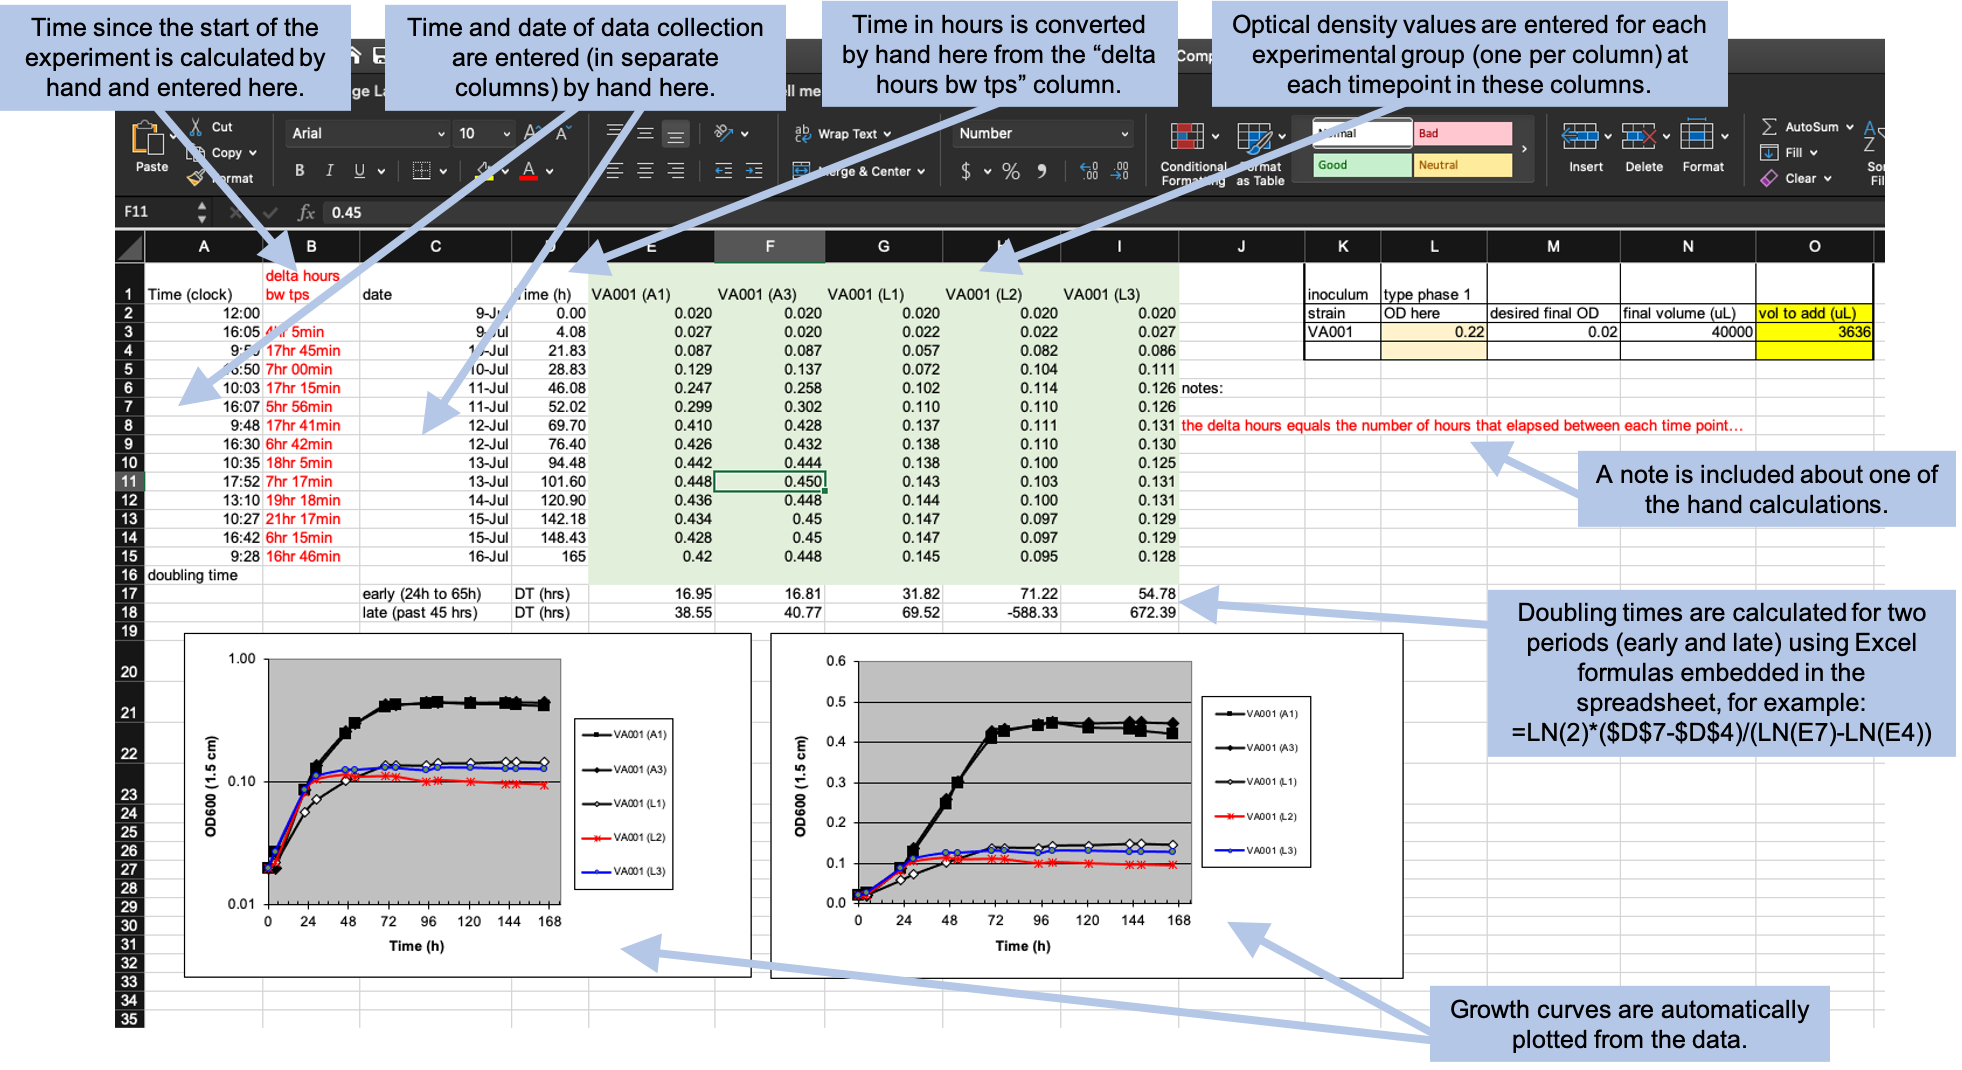
\includegraphics[width=\textwidth]{figures/growth_curve_example} \caption[Example of an Excel spreadsheet used to record and analyze data for a laboratory experiment]{Example of an Excel spreadsheet used to record and analyze data for a laboratory experiment. Annotations highlight where data is entered by hand, where calculations are done by hand, and where embedded Excel formulas are used. The figures are created automatically using values in a specified column.}\label{fig:growthexcel1}
\end{figure*}

These data were collected to measure the compare growth yield and doubling time
of \emph{Mycobacterium tuberculosis} (the bacteria that causes tuberculosis in
humans) under two conditions---high oxygen and low oxygen. In humans, \emph{M.
tuberculosis} can persist for years or decades in granulomas, and the centers of
these granulomas are often hypoxic (low in oxygen). Therefore, it's important to
understand how these bacteria grow in hypoxic conditions.

To conduct this experiment, the researchers used test tubes that were capped
with sealed caps to prevent and air exchange between the contents of the tube
and the environment. Inside the tubes, the amount of oxygen was controlled
by shifting the ratio of the volume of the culture (the liquid with nutrients
in which the M. tuberculosis will grow) versus the volume of air.
In the high oxygen condition, a lower volume of culture was used, which leaves
room for a lot of air in the top of the tube. In the low oxygen condition,
the tube was filled almost to the top with culture, which left very little air
at the top of the tube.

Once the tubes were filled and capped, they were left to grow for about a week.
During this time, the researchers took several measurements to determine the
growth of the bacteria in each tube. To do this, they used a spectrophotometer
to track optical density over time. This method gives a measurement that is
directly proportional to the cell mass in each tube, and so provides a measure
of how much the bacteria has grown since the start of the experiment.

To record data from this experiment, researchers used the spreadsheet shown in
Figure \ref{fig:growthexcel1}. This spreadsheet is an example of a data
collection template---it was created not only for this experiment, but also for
other experiments that this research group conducts to measure bacterial growth
under different conditions. It was designed to allow a researcher working in the
laboratory to record measurements over the course of the experiment.

Let's take a closer look at some of the features of this spreadsheet. First, it
has a section on the top right that focuses on data collection during the
experiment, with one row for each time when the tubes were measured for the cell
mass. This section of the spreadsheet starts with several
columns related to the time of each measurement, including the clock time at
measurement (column A), the difference in time (hours) between each time point
in which data were collected (column B), the date on which data were gathered
(column C), and the time in hours for each data point from the start of the
study for graphing purposes (column D). The columns for clock time (A) and date
(C) were recorded by hand, while the columns for time since the start of the
experiment (B and D) were calculated or converted by hand from these values and
then entered in the column. The remaining columns (E--I) provide data on the
optical density (absorbance at 600 nm), which is directly proportional to cell
mass in the tube. There is one column per test tub, and each of these column
labels includes a test tube ID (A1, A3, L1, L2, L3). If a tube ID starts with
``A'', it was grown in high oxygen conditions, and if it starts with ``L'', it was
grown in low oxygen conditions.

Next, the spreadsheet has areas that provide summaries of the data, calculated
using embedded formulas or through the spreadsheet's plotting functions. For
example, rows 17--18 provide calculations of the doubling time of the bacteria
in each tube for two periods (early and late in the experiment), while two
growth curves are plotted at the bottom of the spreadsheet.

Finally, the spreadsheet includes a couple of other features, including some
written notes about one of the hand calculations and a macro in the top right
that can be used by the researcher to calculate the amount of the initial
inoculum to add to each tube at the start of the experiment.

What the researchers found appealing about the format of this spreadsheet was
the ease with which the researcher collecting data in the laboratory could
accomplish the study goals. The data being graphed in real time, and the
inclusion of a simple macro to calculate doubling time, allowed the research in
the laboratory to see tangible differences between the two assay conditions as
data were collected over the one-week experiment. They also cited the and ease
with which additional sampling data points could be added.

However, many of these features can have undesired consequences. They can increase
the chance of errors in recording the data and in calculating summaries based on the
data. They also make it hard to move the data into a reproducible pipeline, and
so limit opportunities for more sophisticated analysis and visualization. In the
next section of this module, we'll highlight features of data collection templates
like this one that can make data collection untidy. In the next module (module 2.5),
we'll discuss how you could create a new data collection template for this example
data that would be tidier, and use this to open a more general discussion of
principles of tidy data collection templates.

\subsection{Features that make data collection templates untidy}\label{features-that-make-data-collection-templates-untidy}

There are several features of the data collection template shown in Figure
\ref{fig:growthexcel1} that make it untidy. These will make it difficult read
the data into a statistical program like R or Python to conduct data analysis
and visualization. There are also some features that make it prone to errors in
data collection and analysis.

First, these data will be hard to read into a statistical program because the
raw data form only part of the spreadsheet (Figure \ref{fig:extractraw}, area
highlighted by the blue box). The ``extra'' elements on the spreadsheet, which
include the output from calculations, plots, macros, and notes, make it harder
to isolate the raw data from the file when using a statistical program.

\begin{figure*}
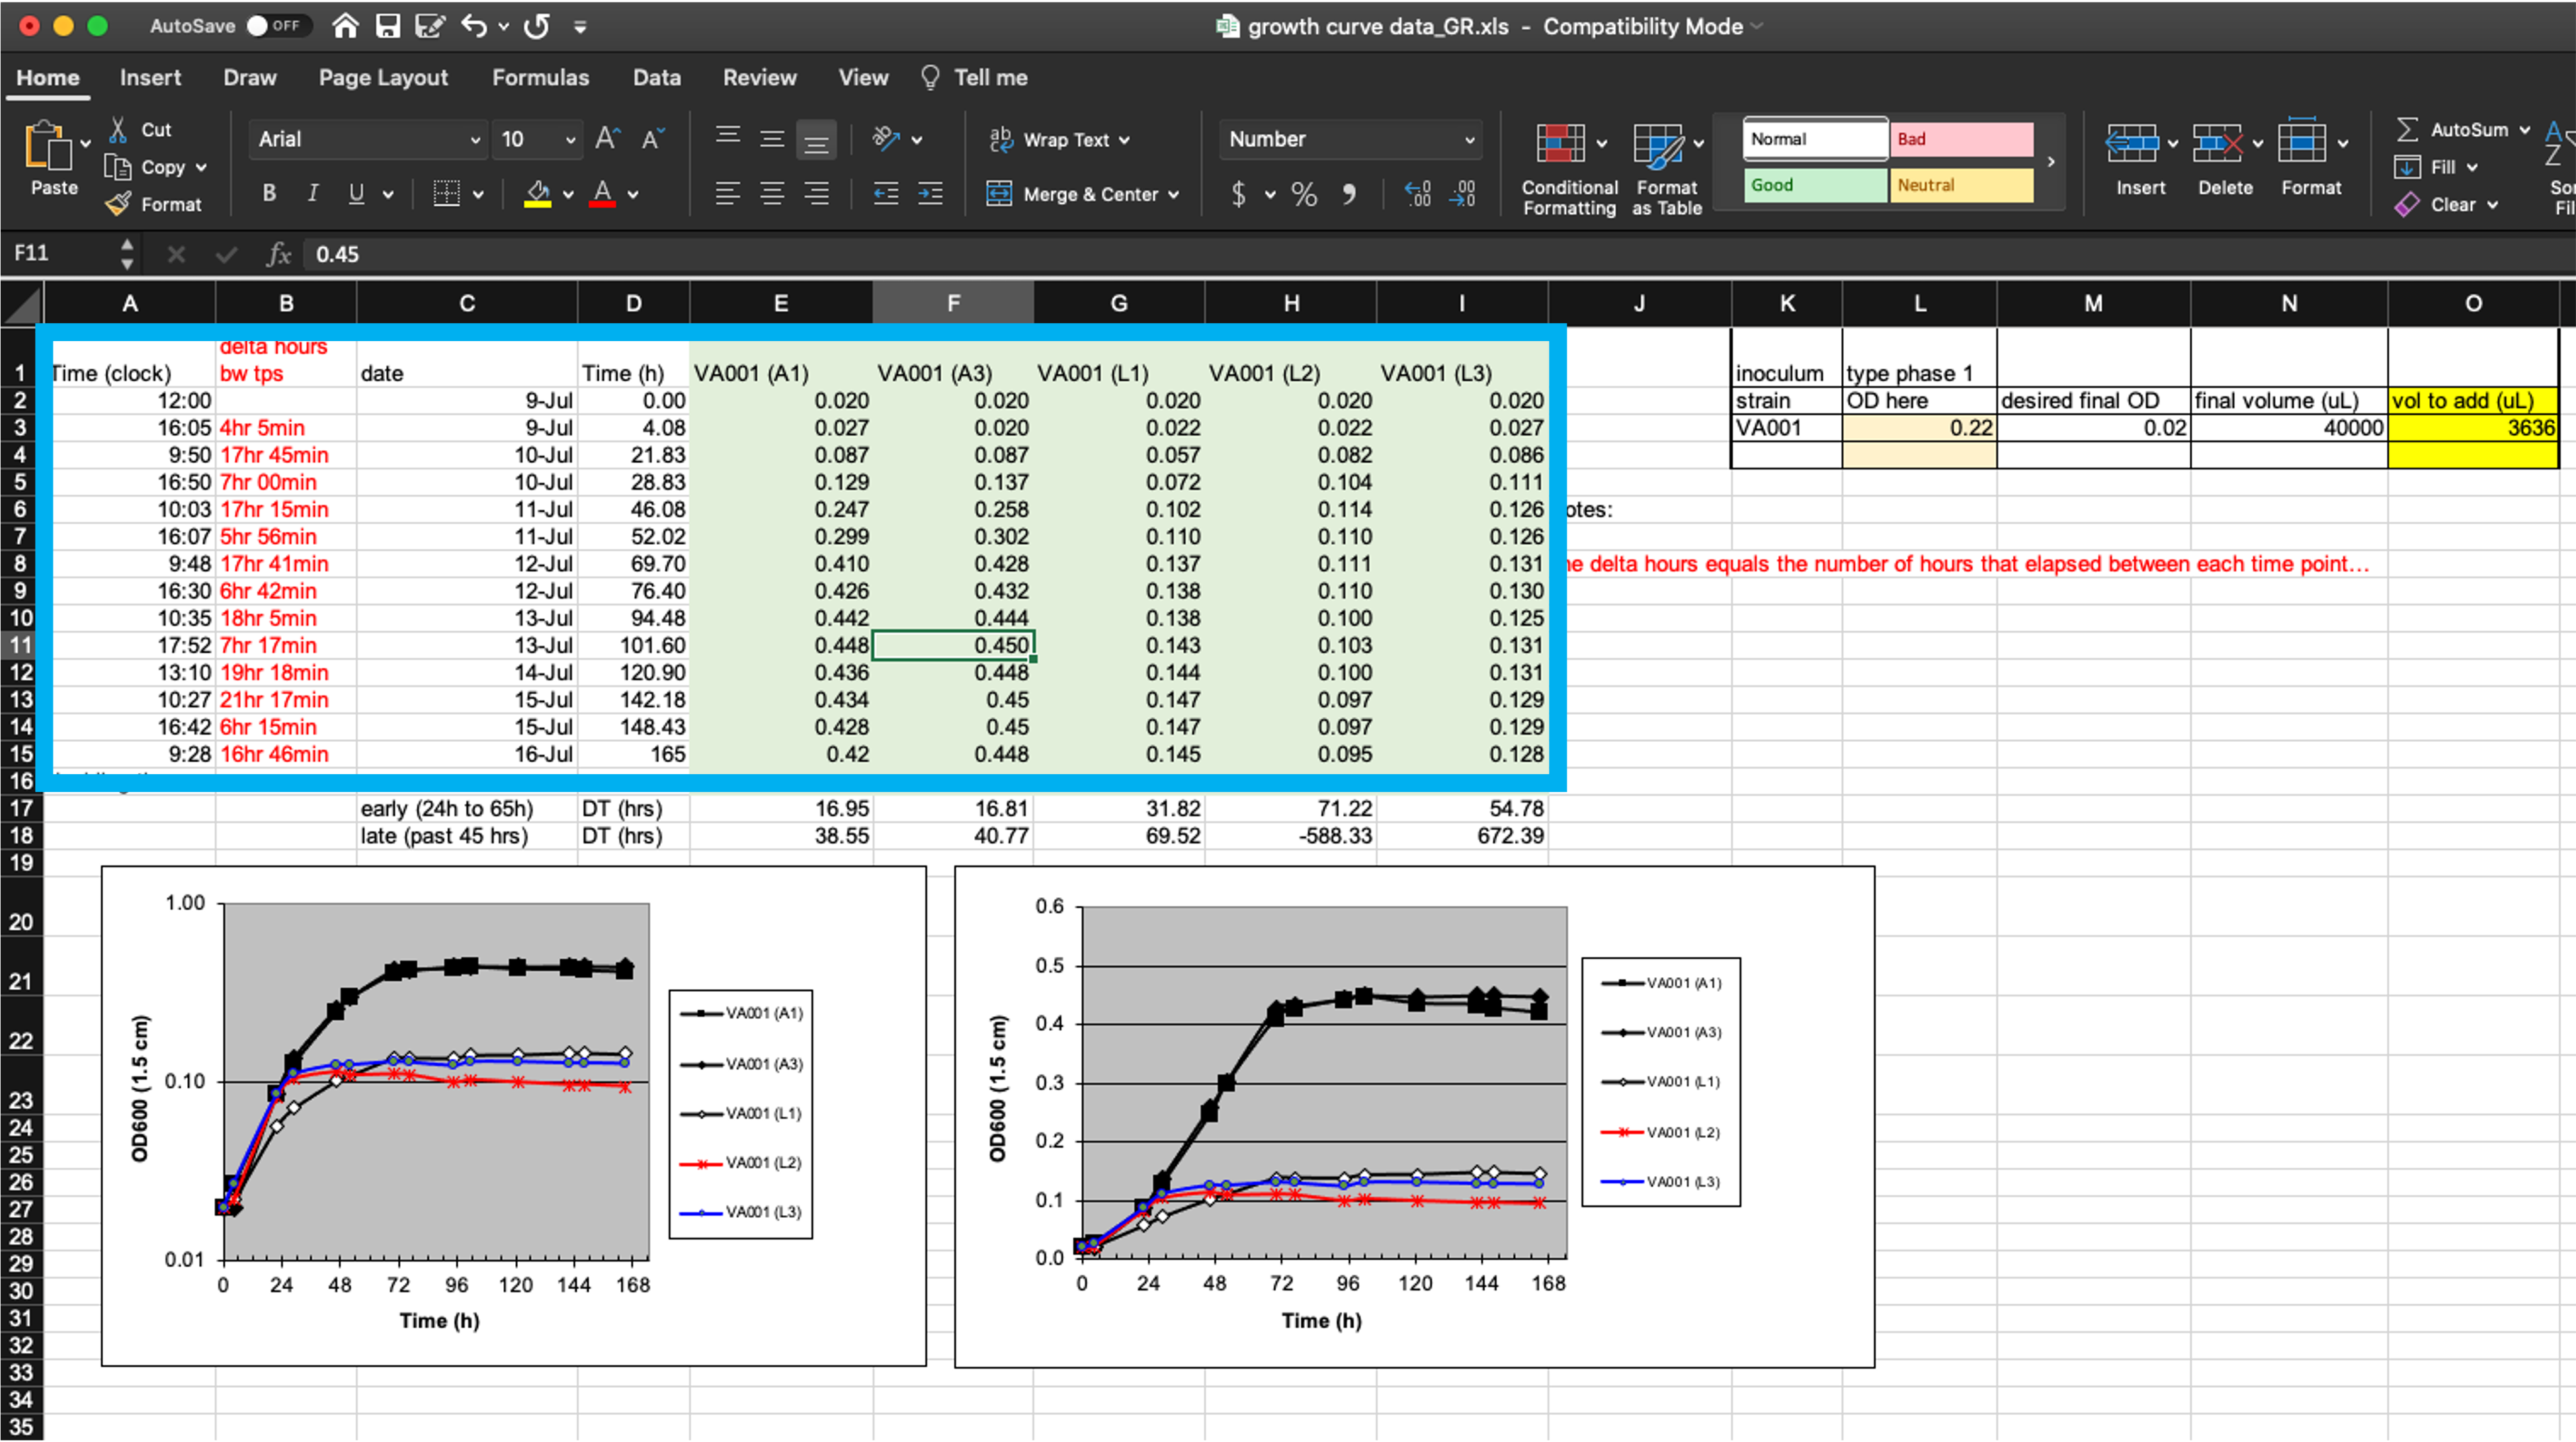
\includegraphics[width=\textwidth]{figures/growth_curve_raw_data} \caption[Isolating raw data collected in a template from extra elements]{Isolating raw data collected in a template from extra elements. The box in this figure highlights the area of the spreadsheet where data are collected. All other elements of the spreadsheet focus on other aims (e.g., summarizing these data, adding notes, macros for experimental design). Those other elements make it difficult to extract the raw data for more advanced analysis and visualization through a statistical program like R, Python, or Perl.}\label{fig:extractraw}
\end{figure*}

While these extra elements make it hard to extract the raw data, it isn't
impossible. Programming languages like R include functions to read data in from
a spreadsheet, and these functions often provide options to specify the sheet of
the file to read in, as well as the rows and columns to read from a specific
sheet. In the example spreadsheet in Figure \ref{fig:extractraw}, for example,
you could specify to read in only rows 1--15 of columns A--I, to focus on the
raw data.

However, one goal of reproducible research is to create tools and pipelines that
are robust---that is, ones that still work as desired when the raw data is
changed in small ways, or even across different raw data files. Therefore, while
we could customize code to read in data from a specific part of a complex
spreadsheet, like that shown in Figure \ref{fig:extractraw}, this customization
would make the code less robust. If we asked the statistical program to read in
rows 1--15 of columns A--I, for example, the code would perform incorrectly if
we later added one more time point to the experiment, or if we tried to use the
same template for an experiment that used more test tubes. If we instead use a
template that only records the raw data, without additional elements, then we
can create more robust tools, since we can write code to read in whatever is in
a spreadsheet, rather than restricting to certain rows and columns.

Next, the example template helps demonstrate how specific ways of recording data
can make the template less tidy. First, let's look at how the template records
the time of each measurement. It does this using four separate columns
(Figure \ref{fig:extractraw}). In column C, the researcher records the date a
measurement was taken, and in Column A he or she records the clock time of the
measurement. The experiment was started, for example, at 12:00 PM (``12:00'' in column A)
on July 9 (``9-Jul'' in column C). These values are entered by hand by the researcher.
Next, these values are used to calculate, for each measurement, how long it had been
since the start of the experiment. This value is recorded in two separate ways---as
hours and minutes in column B and converted into hours and percents of hours (using
decimals) in column D. For example, the second measurement was taken at 4:05 PM
on July 9 (``16:05'' in column A and ``9-Jul'' in column C), which is 4 hours and 5 minutes
after the start of the experiment (``4hr 5min'' in column B) or, since 5 minutes is about
8\% of an hour, 4.08 hours after the start of the experiment (``4.08'' in column D).

\begin{figure}
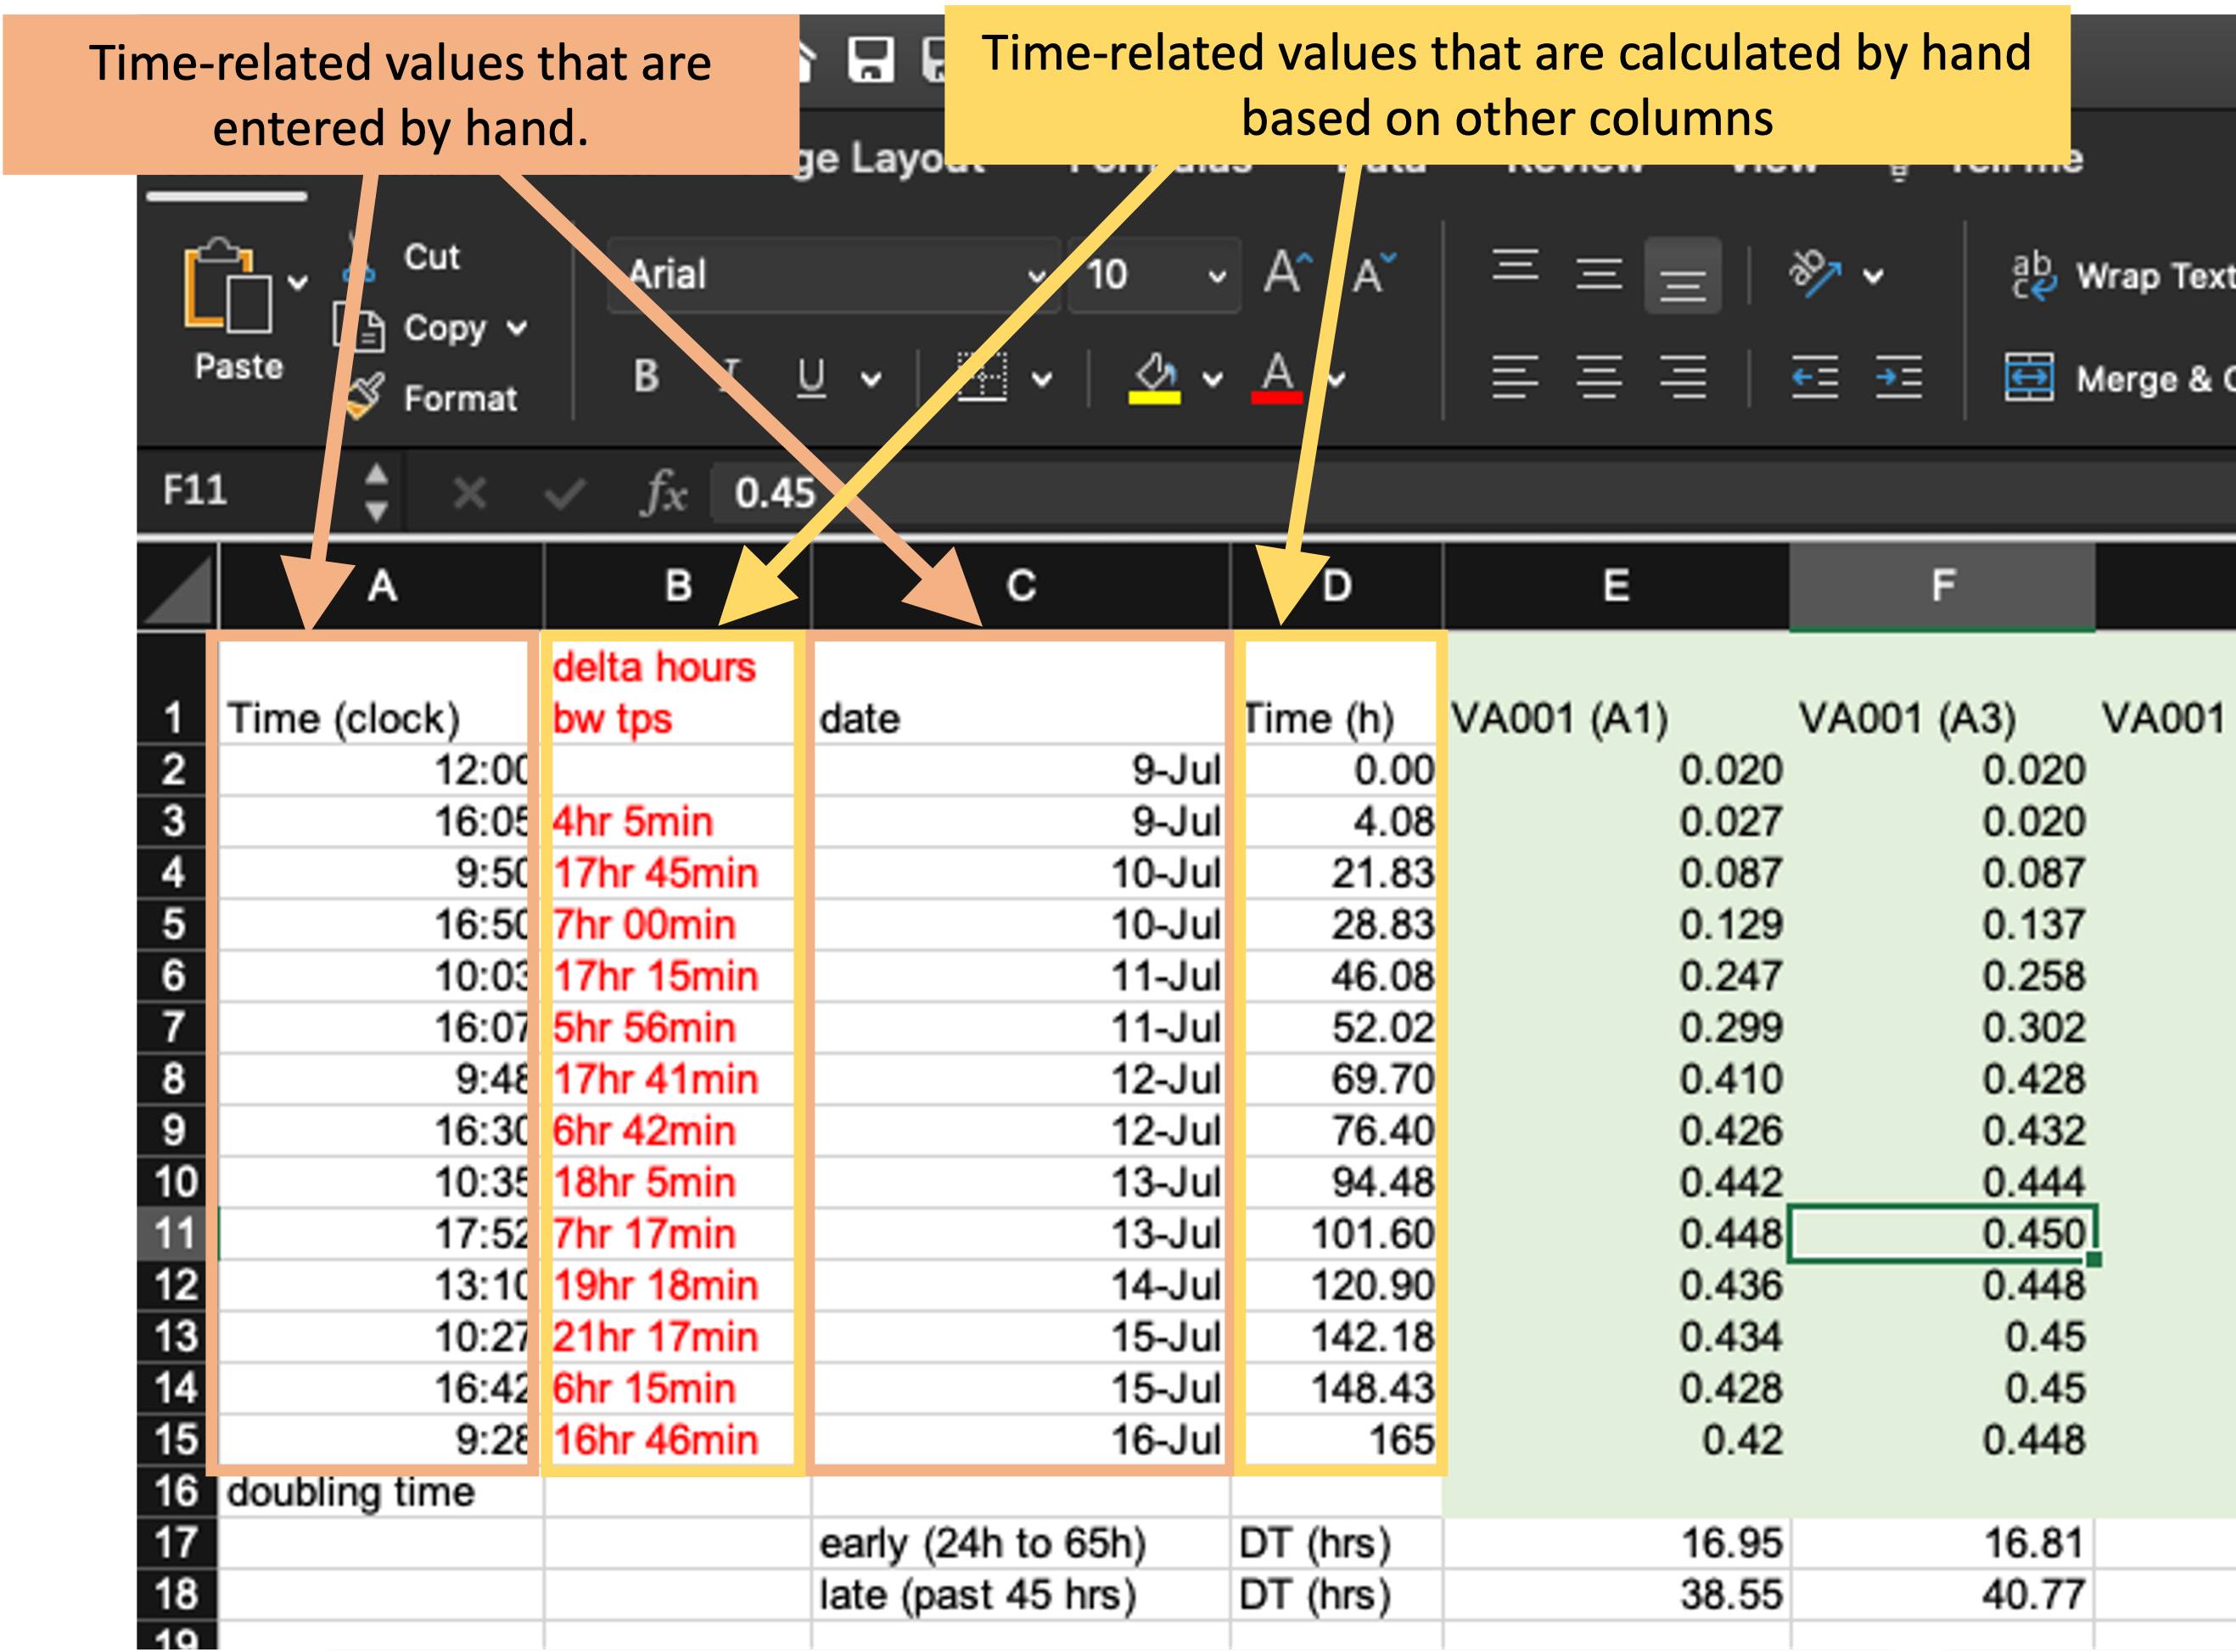
\includegraphics[width=\textwidth]{figures/growth_curve_time_measures} \caption[Measurements of time in the example data collection template]{Measurements of time in the example data collection template. The four highlighted columns (columns A, B, C, and D) are all used in this spreadsheet to record time. The methods of recording time in this template, however, may make it more likely to create errors in data recording and collection and will make it harder to use the data in a reproducible pipeline.}\label{fig:timemeasures}
\end{figure}

There are a few things that could be changed about how the time data are
recorded here that could make this data collection template tidier. First, it
would be better to focus only on recording the raw data, rather than adding
calculations based on that data. Columns B and D in Figure \ref{fig:extractraw}
are both the output from calculations. Anytime a spreadsheet includes a
calculation, it creates the room for mistakes in data collection and analysis.
Often, calculations in a spreadsheet will be done using embedded formulas. These
can cause problems when new columns or rows are added to the data, as that
can shift the cells meant to be used in the calculation. Further, these formulas
are embedded in the spreadsheet, where they can't be seen and checked very
easily, which makes it easy to miss a typo or other error in the formula.

In the example in Figure \ref{fig:extractraw}, columns B and D aren't
calculated by embedded formulas, but rather calculated by the researcher by hand
and then entered. This creates room for user error with each calculation
and data entry. Later, we'll see how we can tidy this data collection
template by removing columns that calculate time (columns B and D) and instead
doing that calculation once the raw data are read into a statistical program.

The second thing that could be changed is how the template records the date and
time of the measurement. Currently, it uses two columns (A and C) to record this
information. However, each piece of information is useless without the
other---instead, they must be known jointly to do things like calculate the time
since the start of the experiment. It would therefore be tidier to record this
information in a single column. For example, instead of recording the starting
time of the experiment as ``12:00'' in column A and ``9-Jul'' in column C, you could
record it as ``July 9, 2019 12:00'' in a single date-time column. In this example,
adding the year (``2019'') to the date will also make this data point easier to
work with in a programming language, as languages like R and Python often have
special functions to work with data in date-time classes, but all elements of
the date and/or time must be included to convert data points into these useful
format.

Next, let's look at how the template collects data related to cell growth in
each tube (columns E--I, Figure \ref{fig:growthmeasures}). These data are
recorded in a format that will work pretty well. Strictly speaking, they aren't
fully tidy (module 2.3), since the column headers include information that we
might want to use as variables in analysis and visualization. Specifically, each
test tube's ID is incorporated in the column name where measurements for that
tube are recorded, since each test tube is recorded using a separate column.

\begin{figure*}
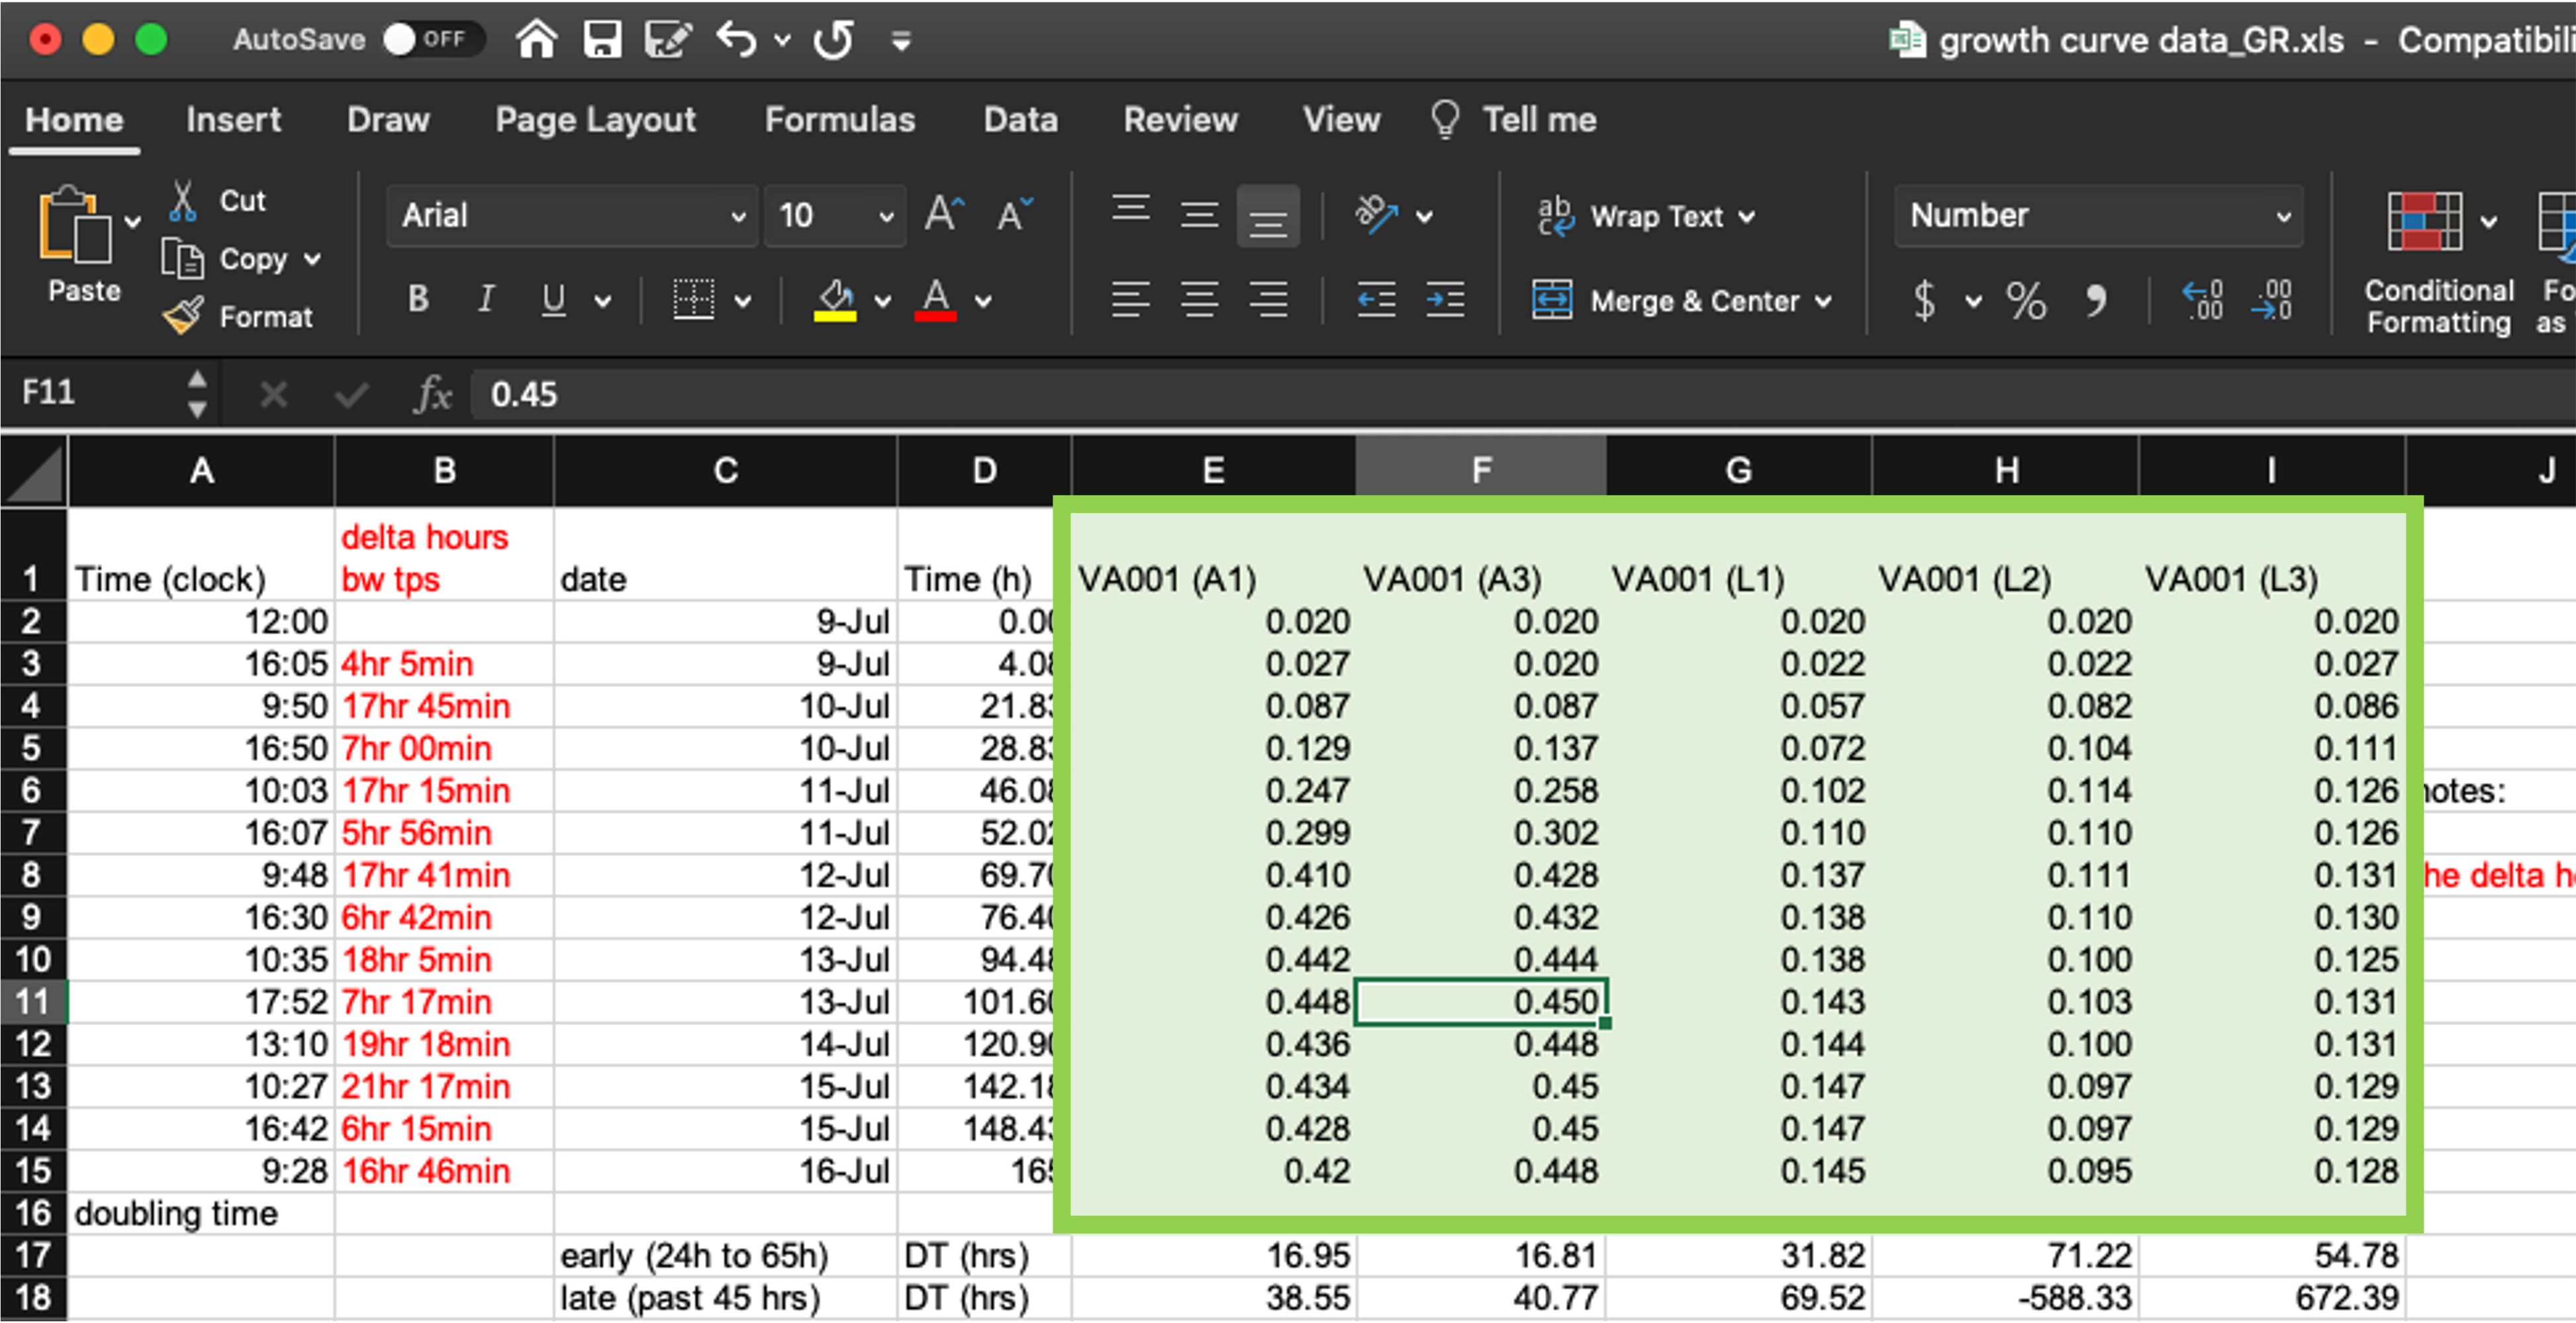
\includegraphics[width=\textwidth]{figures/growth_curve_growth_measures} \caption[Measurements of bacterial growth in the example data collection template]{Measurements of bacterial growth in the example data collection template. The five highlighted columns (columns E--I) are all used in this spreadsheet to record optical density in each test tube at each measurement time.}\label{fig:growthmeasures}
\end{figure*}

If we want to run analysis where we estimate values for each test tube, or
create plots where each test tube's measurements are shown with a separate line,
then once we read the data into another program, we'll need to convert the
format of the data a bit. However, that's quite easy to do in more statistical
programming languages now, and so it's reasonable to compromise on this element
of ``tidiness'' in the data collection format. As we'll show in the next module,
changing this layout in the original data collection would require the
researcher to re-type the measurement date and time several times and would
result in the spreadsheet being longer, and so harder to see at once when
recording data.

There is a final element we'd like to highlight on this example template that
could make the data hard to integrate into a reproducible pipeline. There are
cases in the example template where either column names or cell values are
formatted in a way that would be hard to work with when the data is read into a
program like R or Python (Figure \ref{fig:growthformatting}). For
example, the column names include spaces and parentheses (e.g., ``Time (clock)'').
If left as-is, when the data are read into another program, the column names
will need to be cleaned up to take these characters out, so that the column
names are composed only of alphabetical characters, numbers, or underscores.
While this can be done in code like R or Python, it will add to the data
cleaning process and could be avoided by using simpler column names in the
original data collection template.

\begin{figure*}
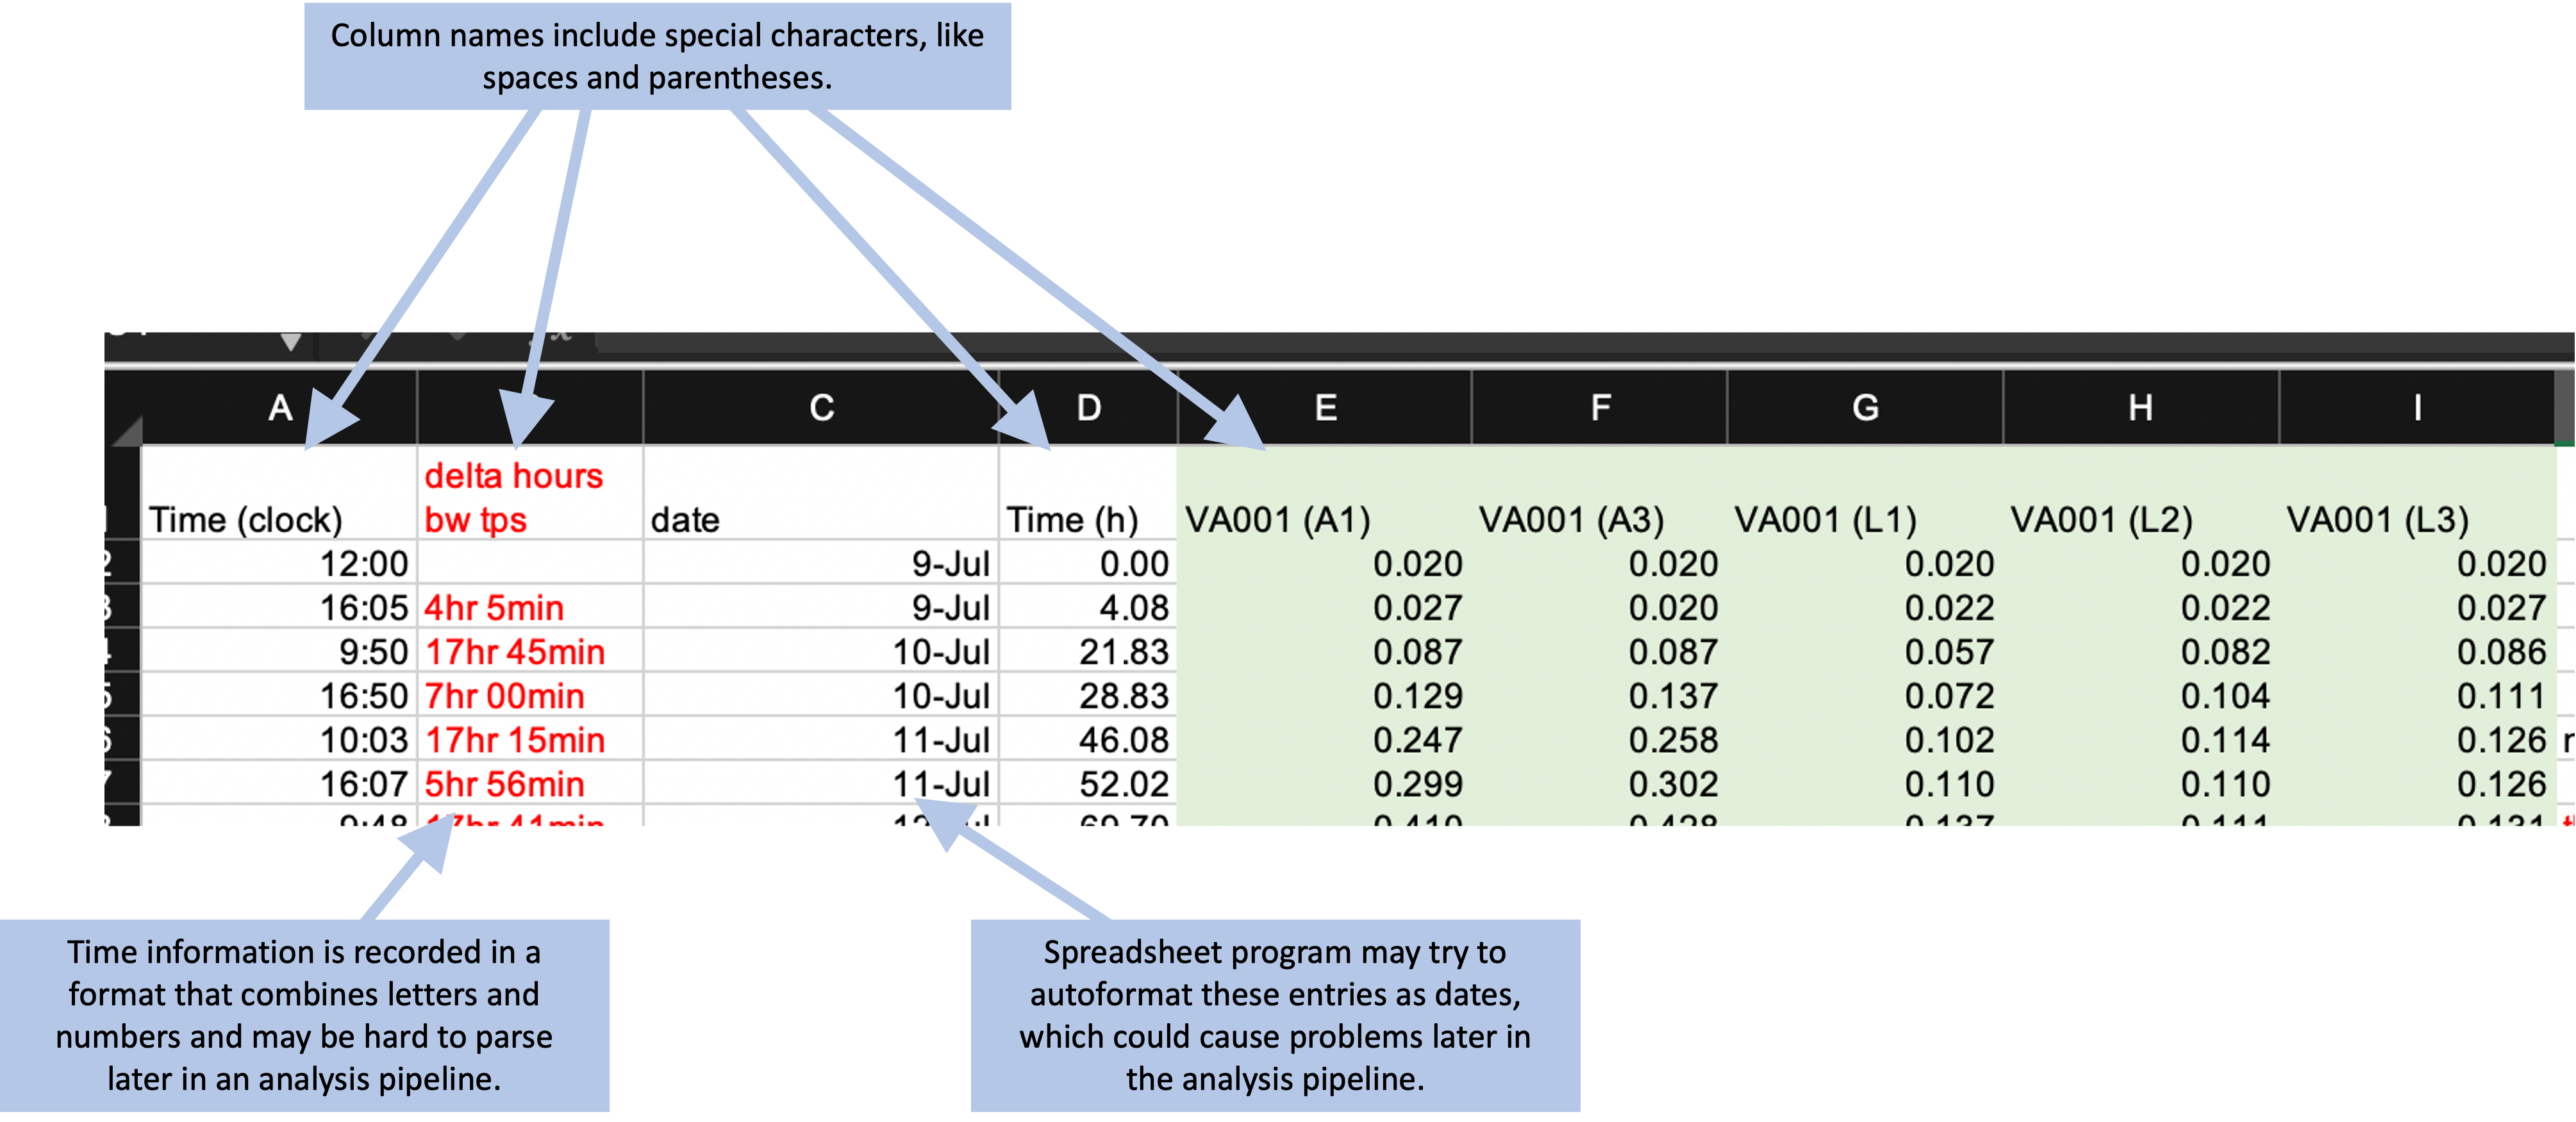
\includegraphics[width=\textwidth]{figures/growth_curve_formatting} \caption[Examples of special characters and formatting in the example template that could cause problems later in a data analysis pipeline]{Examples of special characters and formatting in the example template that could cause problems later in a data analysis pipeline.}\label{fig:growthformatting}
\end{figure*}

\subsection{Converting to a ``tidier'' format for data collection templates}\label{converting-to-a-tidier-format-for-data-collection-templates}

Now that we've looked at characteristics that can make a data collection
template untidy, let's go through some principles for creating tidy templates to
record the same data. In this module, we'll focus on higher-level strategies,
using the example data collection template to highlight out points. In the
next module (module 2.5), we'll provide a detailed walk-through of how the
example template can be modified to use a tidier format.

There are three basic principles for designing tidy templates that will go a
long way to creating ways to collect data in a research group that can be easily
used within a reproducible analysis pipeline. The first principle in designing a
tidier template for collecting laboratory data is to \textbf{limit the template to the
collection of data}. The key here is the word ``collection''. A tidy template
will avoid any calculations done on the original data and instead focus only on
the initial data that the researcher records for the experiment. This means that
you should exclude from the template any element that provides a calculation,
summary, or plot based on the initial recorded element. You should also exclude
any special formatting that you are using to encode information. For example,
say that you are collecting data, and in some cases you get a warning that the
reading may be below the instrument's detection limit. It may be tempting to
highlight the cells with measurements where this warning was displayed as you
record the data. However, you should avoid doing this, as any color or other
formatting information will be lost when you read the data in the file into a
statistical program. Instead, you could add a second column to indicate if the
measurement included a warning.

The second principle is to \textbf{make sensible choices when dividing data collection
into rows and columns}. There are many different ways that you could spread the
data collection into rows and columns. One decision is how (and whether) to
divide recorded information across columns. Figure \ref{fig:arrangingcolumns},
for example, shows several ways that you could divide data on a date and time
into one or more columns. In this example, it typically makes the most sense to
use a single column to record all the date and time elements (the top example in
Figure \ref{fig:arrangingcolumns}). As mentioned earlier, most statistical
programs have powerful functions for parsing dates and times, after which they
store these data in special classes that allow time-related operations (for
example, calculating the time difference between two date-time measurements). It
will be most efficient to record all date and time elements in a single column.

\begin{figure*}
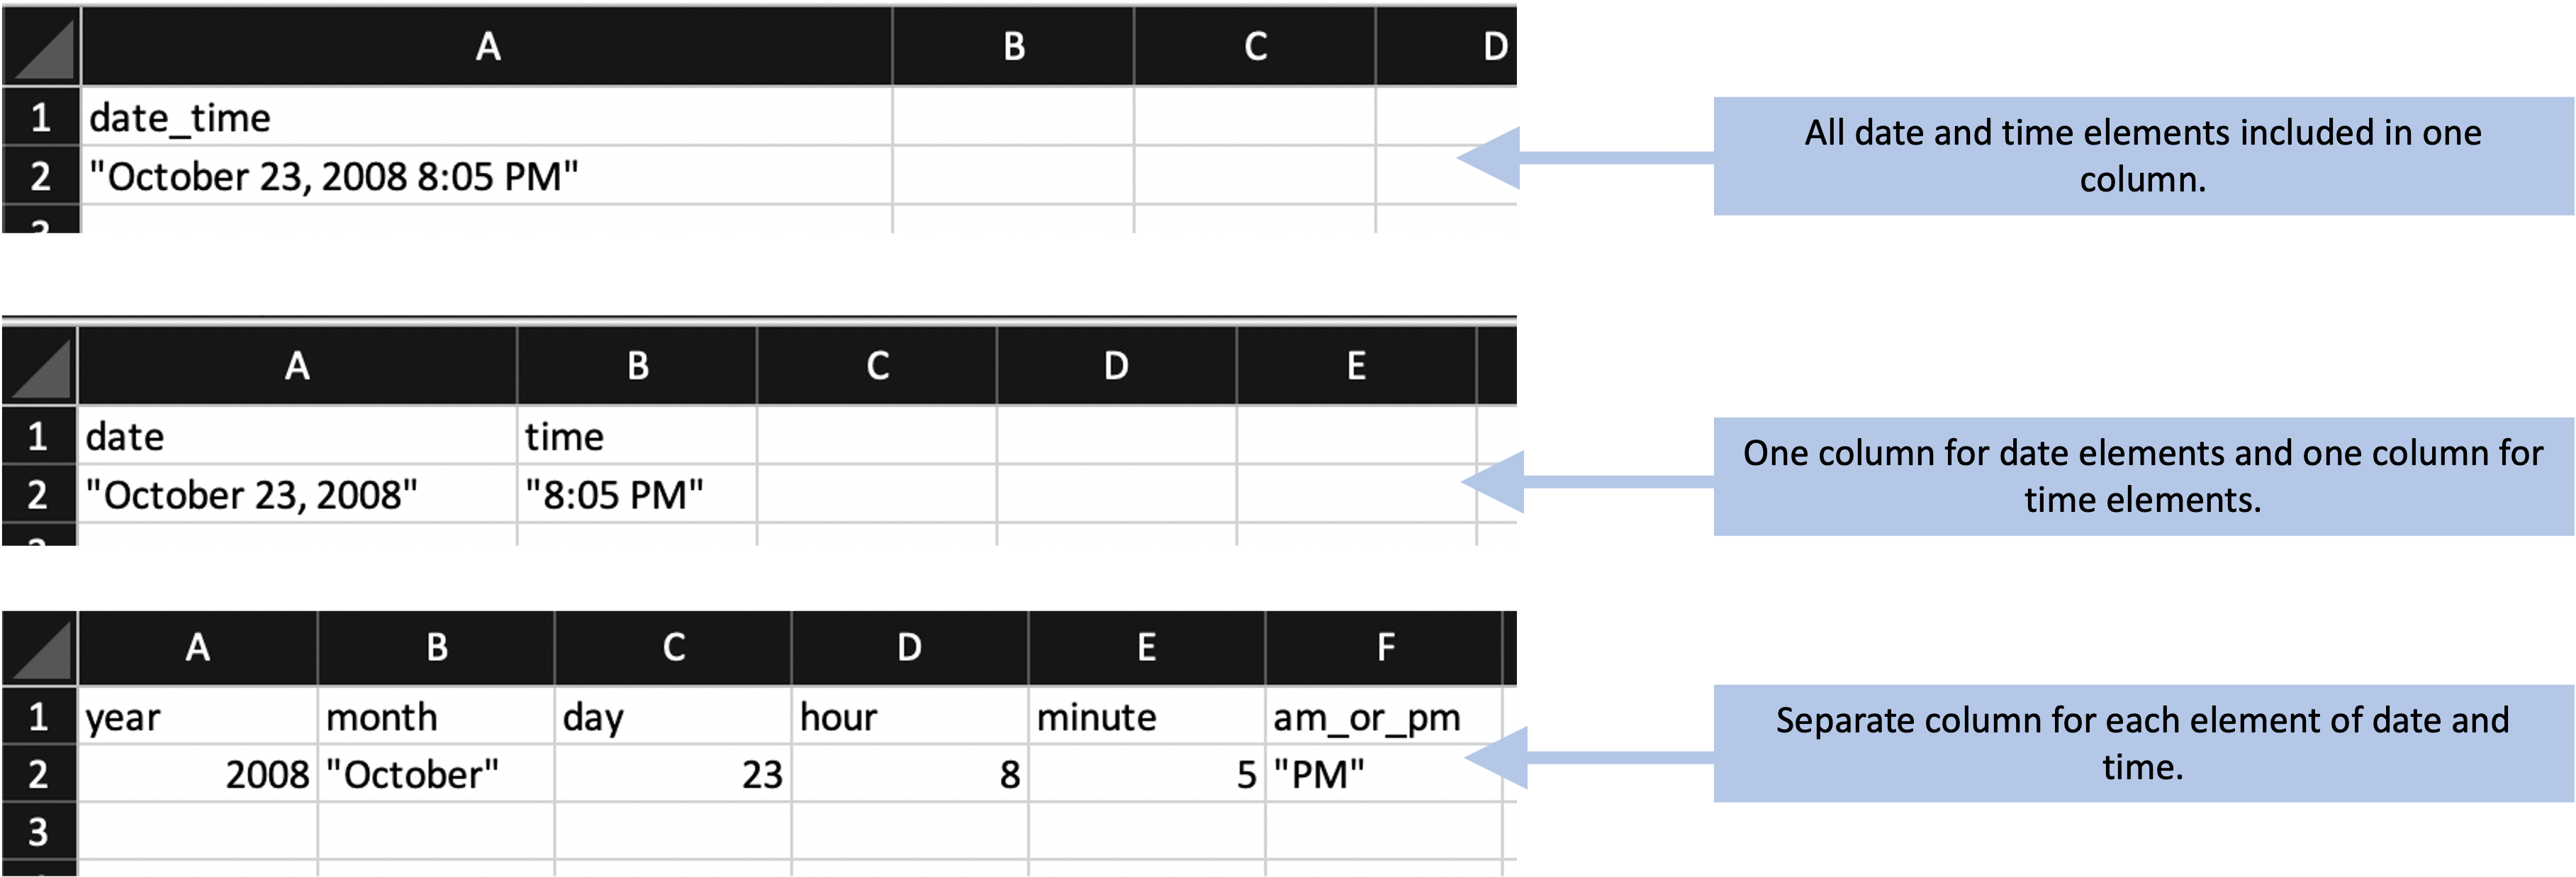
\includegraphics[width=\textwidth]{figures/arranging_columns} \caption[Examples of special characters and formatting in the example template that could cause problems later in a data analysis pipeline]{Examples of special characters and formatting in the example template that could cause problems later in a data analysis pipeline.}\label{fig:arrangingcolumns}
\end{figure*}

Conversely if you have complex data with different elements (for example, height
in components of inches and feet), it may make sense to use separate columns for
each of the components. For example, rather than using one column to record
\texttt{5\textquotesingle{}7"}, you could divide the information into one column with the component that
is in feet (\texttt{5}) and one with the component in inches (\texttt{7}). In the first case
(recording \texttt{5\textquotesingle{}7"}), when you read the data into a program like R you would need
to use complex code to split the value into its parts to be able to use it. In
the second case, you could easy work with the values in the two separate columns
to calculate a value to use in further work (e.g., use a formula like \texttt{height\_ft\ *\ 12\ +\ height\_in} to calculate the full height in inches).

Another decision at this stage is how ``long'' versus ``wide'' you make your
template. A ``wide'' design will include more columns, while a ``long'' design will
include more rows. Often, you can create different designs that allow you to
collect the same values but with different designs along this wide-versus-long
spectrum. Figure \ref{fig:longversuswide} gives two examples of templates that
collect the same data, but one is using a wider design and the other is using a
longer design.

\begin{figure*}
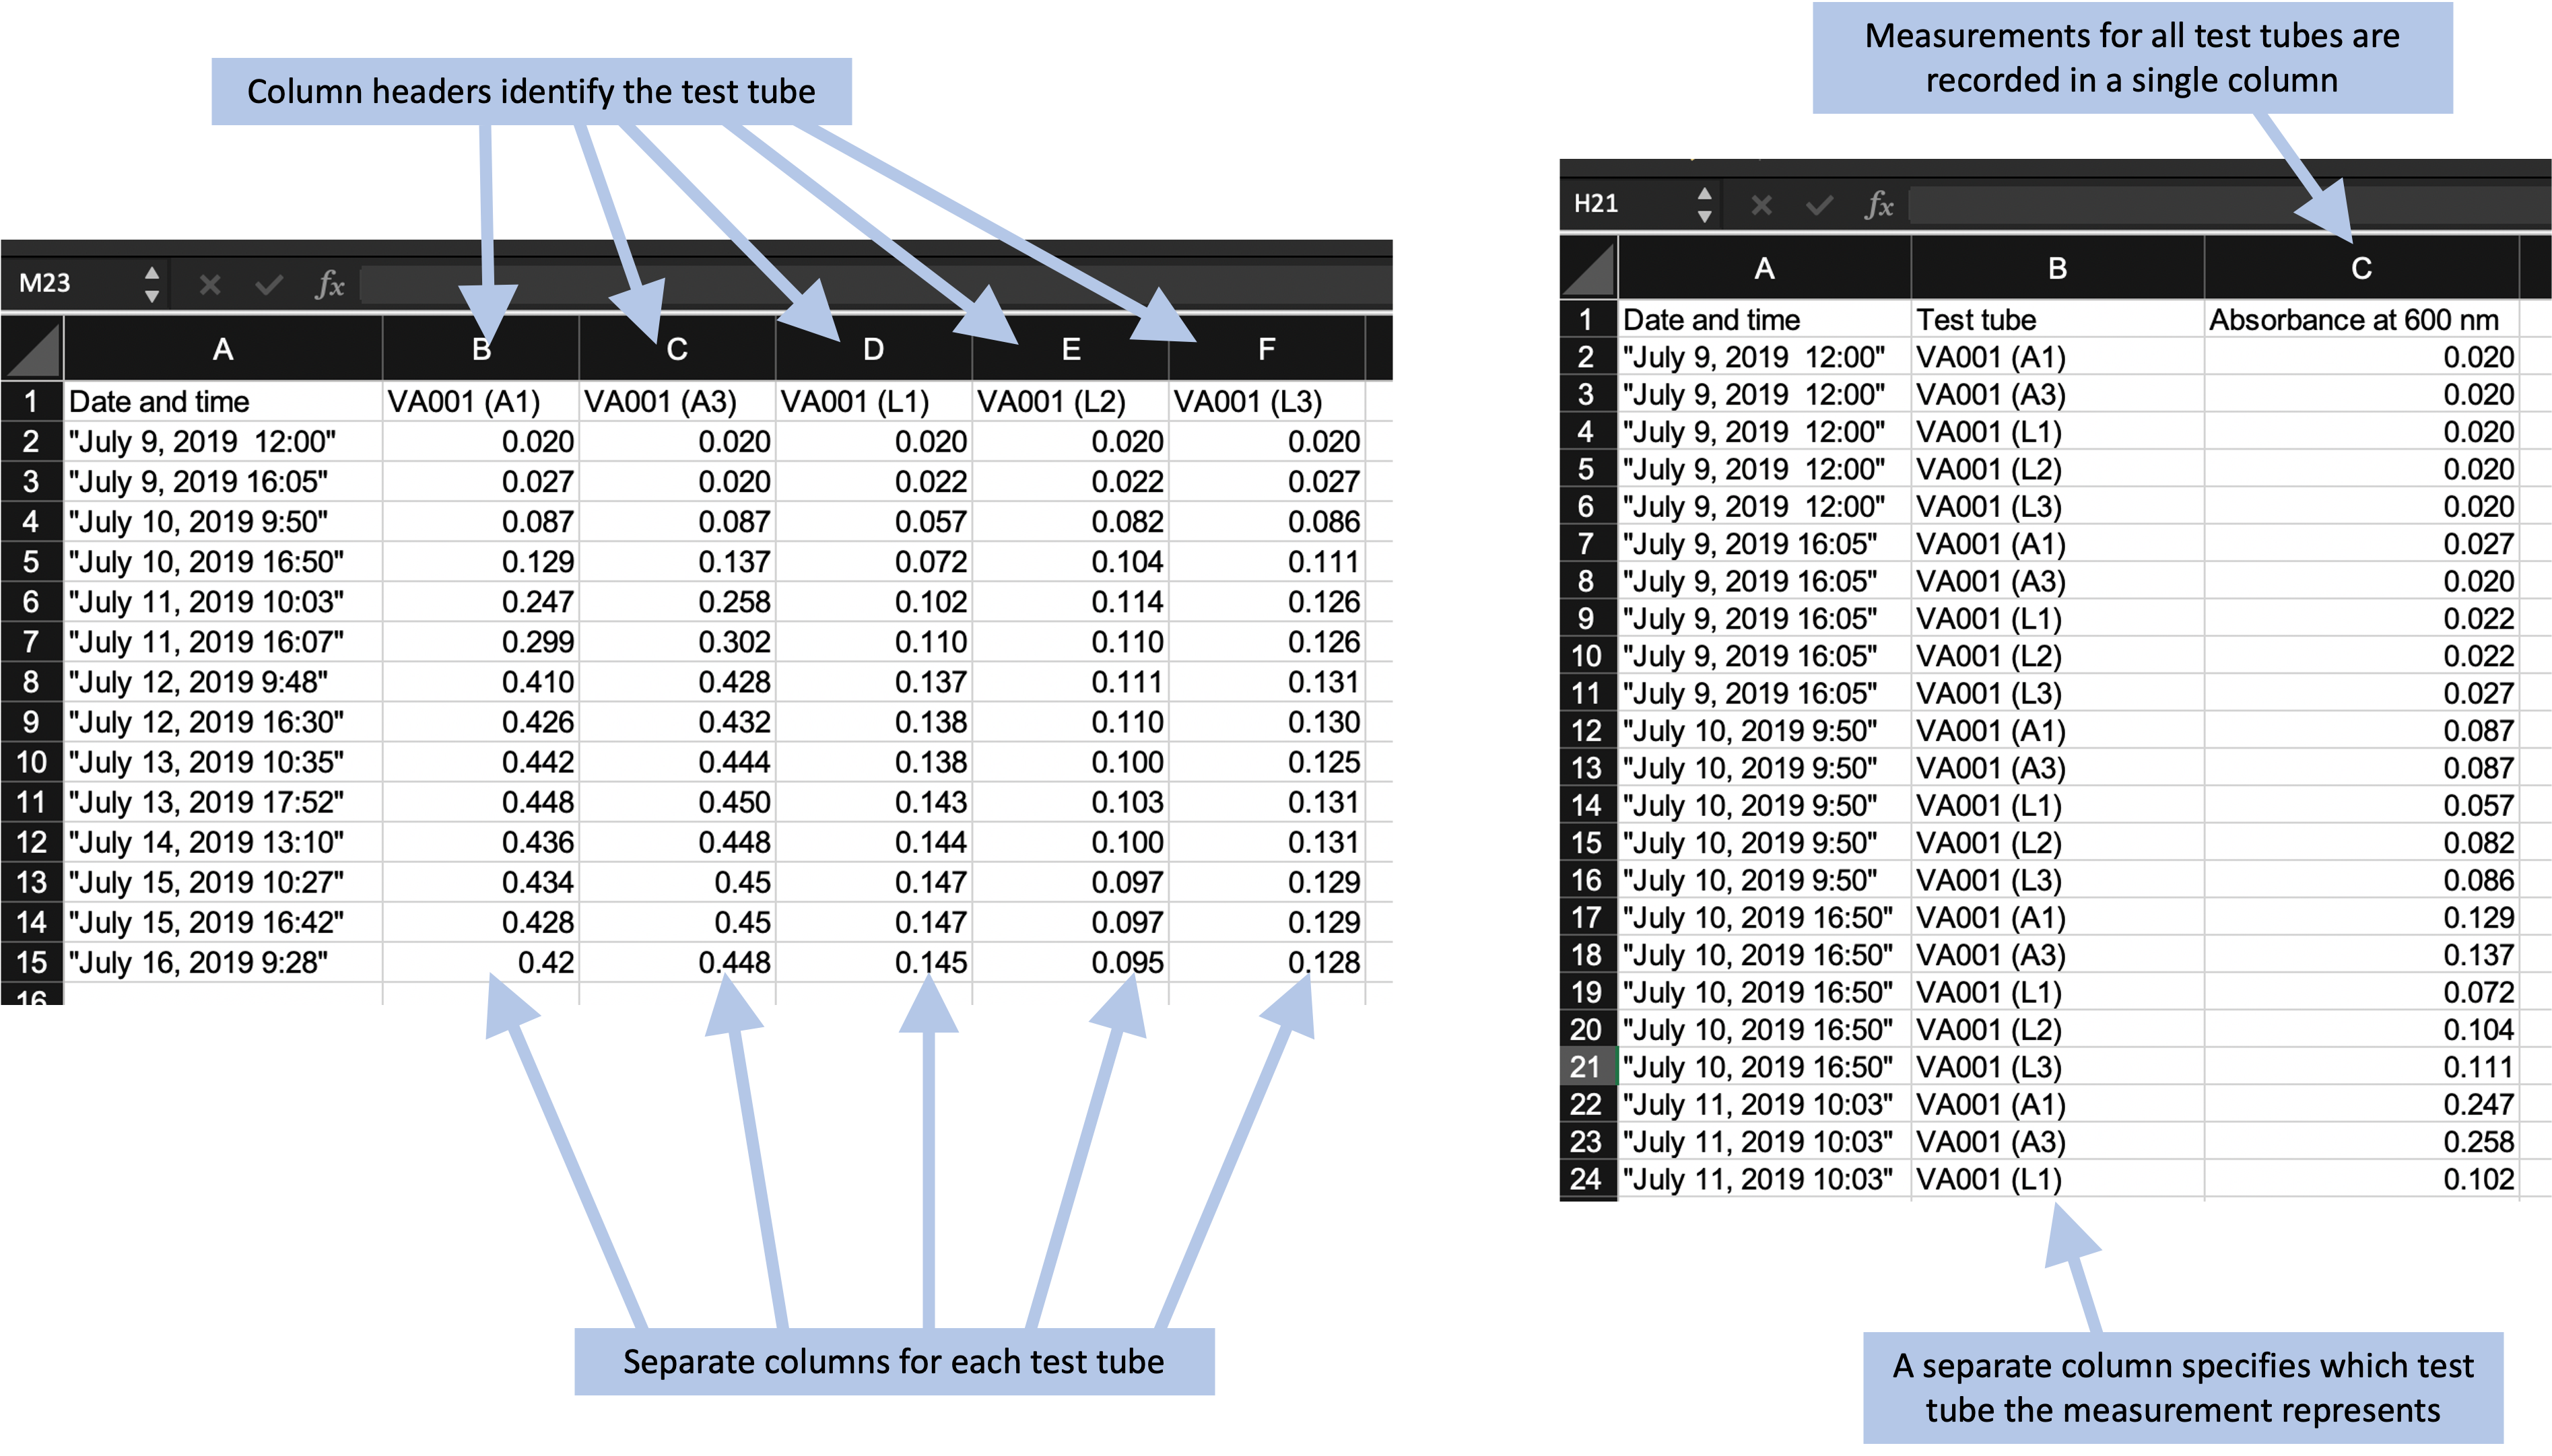
\includegraphics[width=\textwidth]{figures/growth_curve_long_vs_wide} \caption[Examples of two ways arranging the same data in a data recording template]{Examples of two ways arranging the same data in a data recording template. The format on the left records the optical density measurements for each test tube in a separate column, and the column header identifies the test tube. This is an example of a 'wider' format. The format on the right records the optical density for all test tupbes in a single column, using a separate column to record which test tube the measurement represents. This is an example of a 'longer' format.}\label{fig:longversuswide}
\end{figure*}

In module 2.3, we described the rules for the tidy format for dataframes.
If you record data directly into a tidy format, it will be very easy to
read into a programming language to analyze and visualize. However,
this tidy format can sometimes result in datasets that are very long. It
may be more convenient to record data in a wider format, especially if you
are recording the data in a laboratory setting where it is inconvenient to
scroll up and down within a longer-format spreadsheet as you record.

Fortunately, there are some convenient tools in programs like R and Python that
can be used to take data that are collected in a wider format and reformat them
to the tidy format as soon as they are read into the software program. While
this will require some extra code, it is usually code that is fairly simple and
straightforward. Therefore, when you design your data collection template, you
can balance any practical advantages of using a wider data collection format
against the advantages of a fully tidy format that apply once your input the
data into a statistical program for analysis and visualization. Often, the wider
format might win out in this balance, and that's fine.

The third principle is to \textbf{avoid characters or formatting that will make it
hard for a computer program to process the data}. This principle is
particularly important for the column names for each column. When you read data
into a statistical program like R, these names will automatically be used as the
column names in the R data frame object, and the code will regularly use these
column names to refer to parts of the data when analyzing and visualizing it.
You will find it easiest to use the data in a reproducible pipeline if you
follow a couple rules for the column names. The reason that these rules will help
is that they replicate the rules for naming objects in programming languages,
and so will help in seamlessly transitioning between the stages of data
collection and data analysis. First, always start a column name with a letter.
Second, only use letters, numbers, or the underscore character (``\_``) for
the rest of the characters in the column name.

Based on these rules, then, you should avoid putting spaces in your column names
when you design a data collection template. It is tempting to include spaces to
make the names clearer for humans to read, and this is understandable. Often,
an underscore serves the same function, allowing for easy human comprehension
while still avoiding characters that are difficult for statistical programs.
For example, if you have a column named ``Optical density'', you can change it
to ``Optical\_density'' without making it much more difficult for a person to
understand. As with other choices in designing a data collection template,
these choices about column names can be a balance between making the template
easy for researchers to use in the laboratory and easy for the statistical
program to parse later in the pipeline. For example, statistical programs like
R have functions for working with character strings that can be used to
replace all the spaces in column names with another character. However, if
it isn't unreasonable to follow the recommended rules in writing column names
for the data collection template, you can keep code later in the pipeline
much simpler, so it's worth considering.

Beyond spaces, there are a number of other special characters that you might
be tempted to include in column names. These could include parentheses, dollar signs,
percent signs, hash marks (``\#''), and so on. Any of these will require extra code
in later steps of an analysis pipeline, and some can cause more severe problems
because they have special meanings in the programming language. For example,
hash marks are used in the R programming language to add comments within code, while
dollar signs are used for subsetting elements of a list or data frame object.
It is worth the effort to avoid all these characters in column names in a data
collection template.

There are also considerations you can make in terms of how you record data within
cells of the data collection template, and these can make a big difference in terms
of how hard or easy it is to work with the data within a statistical program. While
statistical programs like R are very powerful in terms of being able to handle even
very ``messy'' input data, they require a lot of code to leverage this power. By being
thoughtful when you design the template to record the data, you can avoid having to
use a lot of code to input and clean the data in later stages of the pipeline.

Figure \ref{fig:recordingtime} gives an example of a choice that you could make
in the format you use to record data. This figure shows two columns from the
original data collection template from the example experiment for this module.
This template includes two columns that record the time since the start of the
experiment, and they use different formats for doing this. In column B, time is
recorded in hours and minutes, with the characters ``hr'' and ``min'' used to
separate the two time components. In column D, the same information is recorded,
but in decimals of hours (e.g., 4.08 hours for 4 hours and 5 minutes). While the
format in column B is more similar to how humans think of time, it will take
more code to parse in a statistical program. When reading this data into a
program like R, you would need to use regular expressions to split apart the
different elements and then recombine them into a format that the program
understands. By contrast, the values recorded in column D could be easily read
in by a statistical program, with minimal code needed before they could be used
in analysis and visualizations.

\begin{figure}
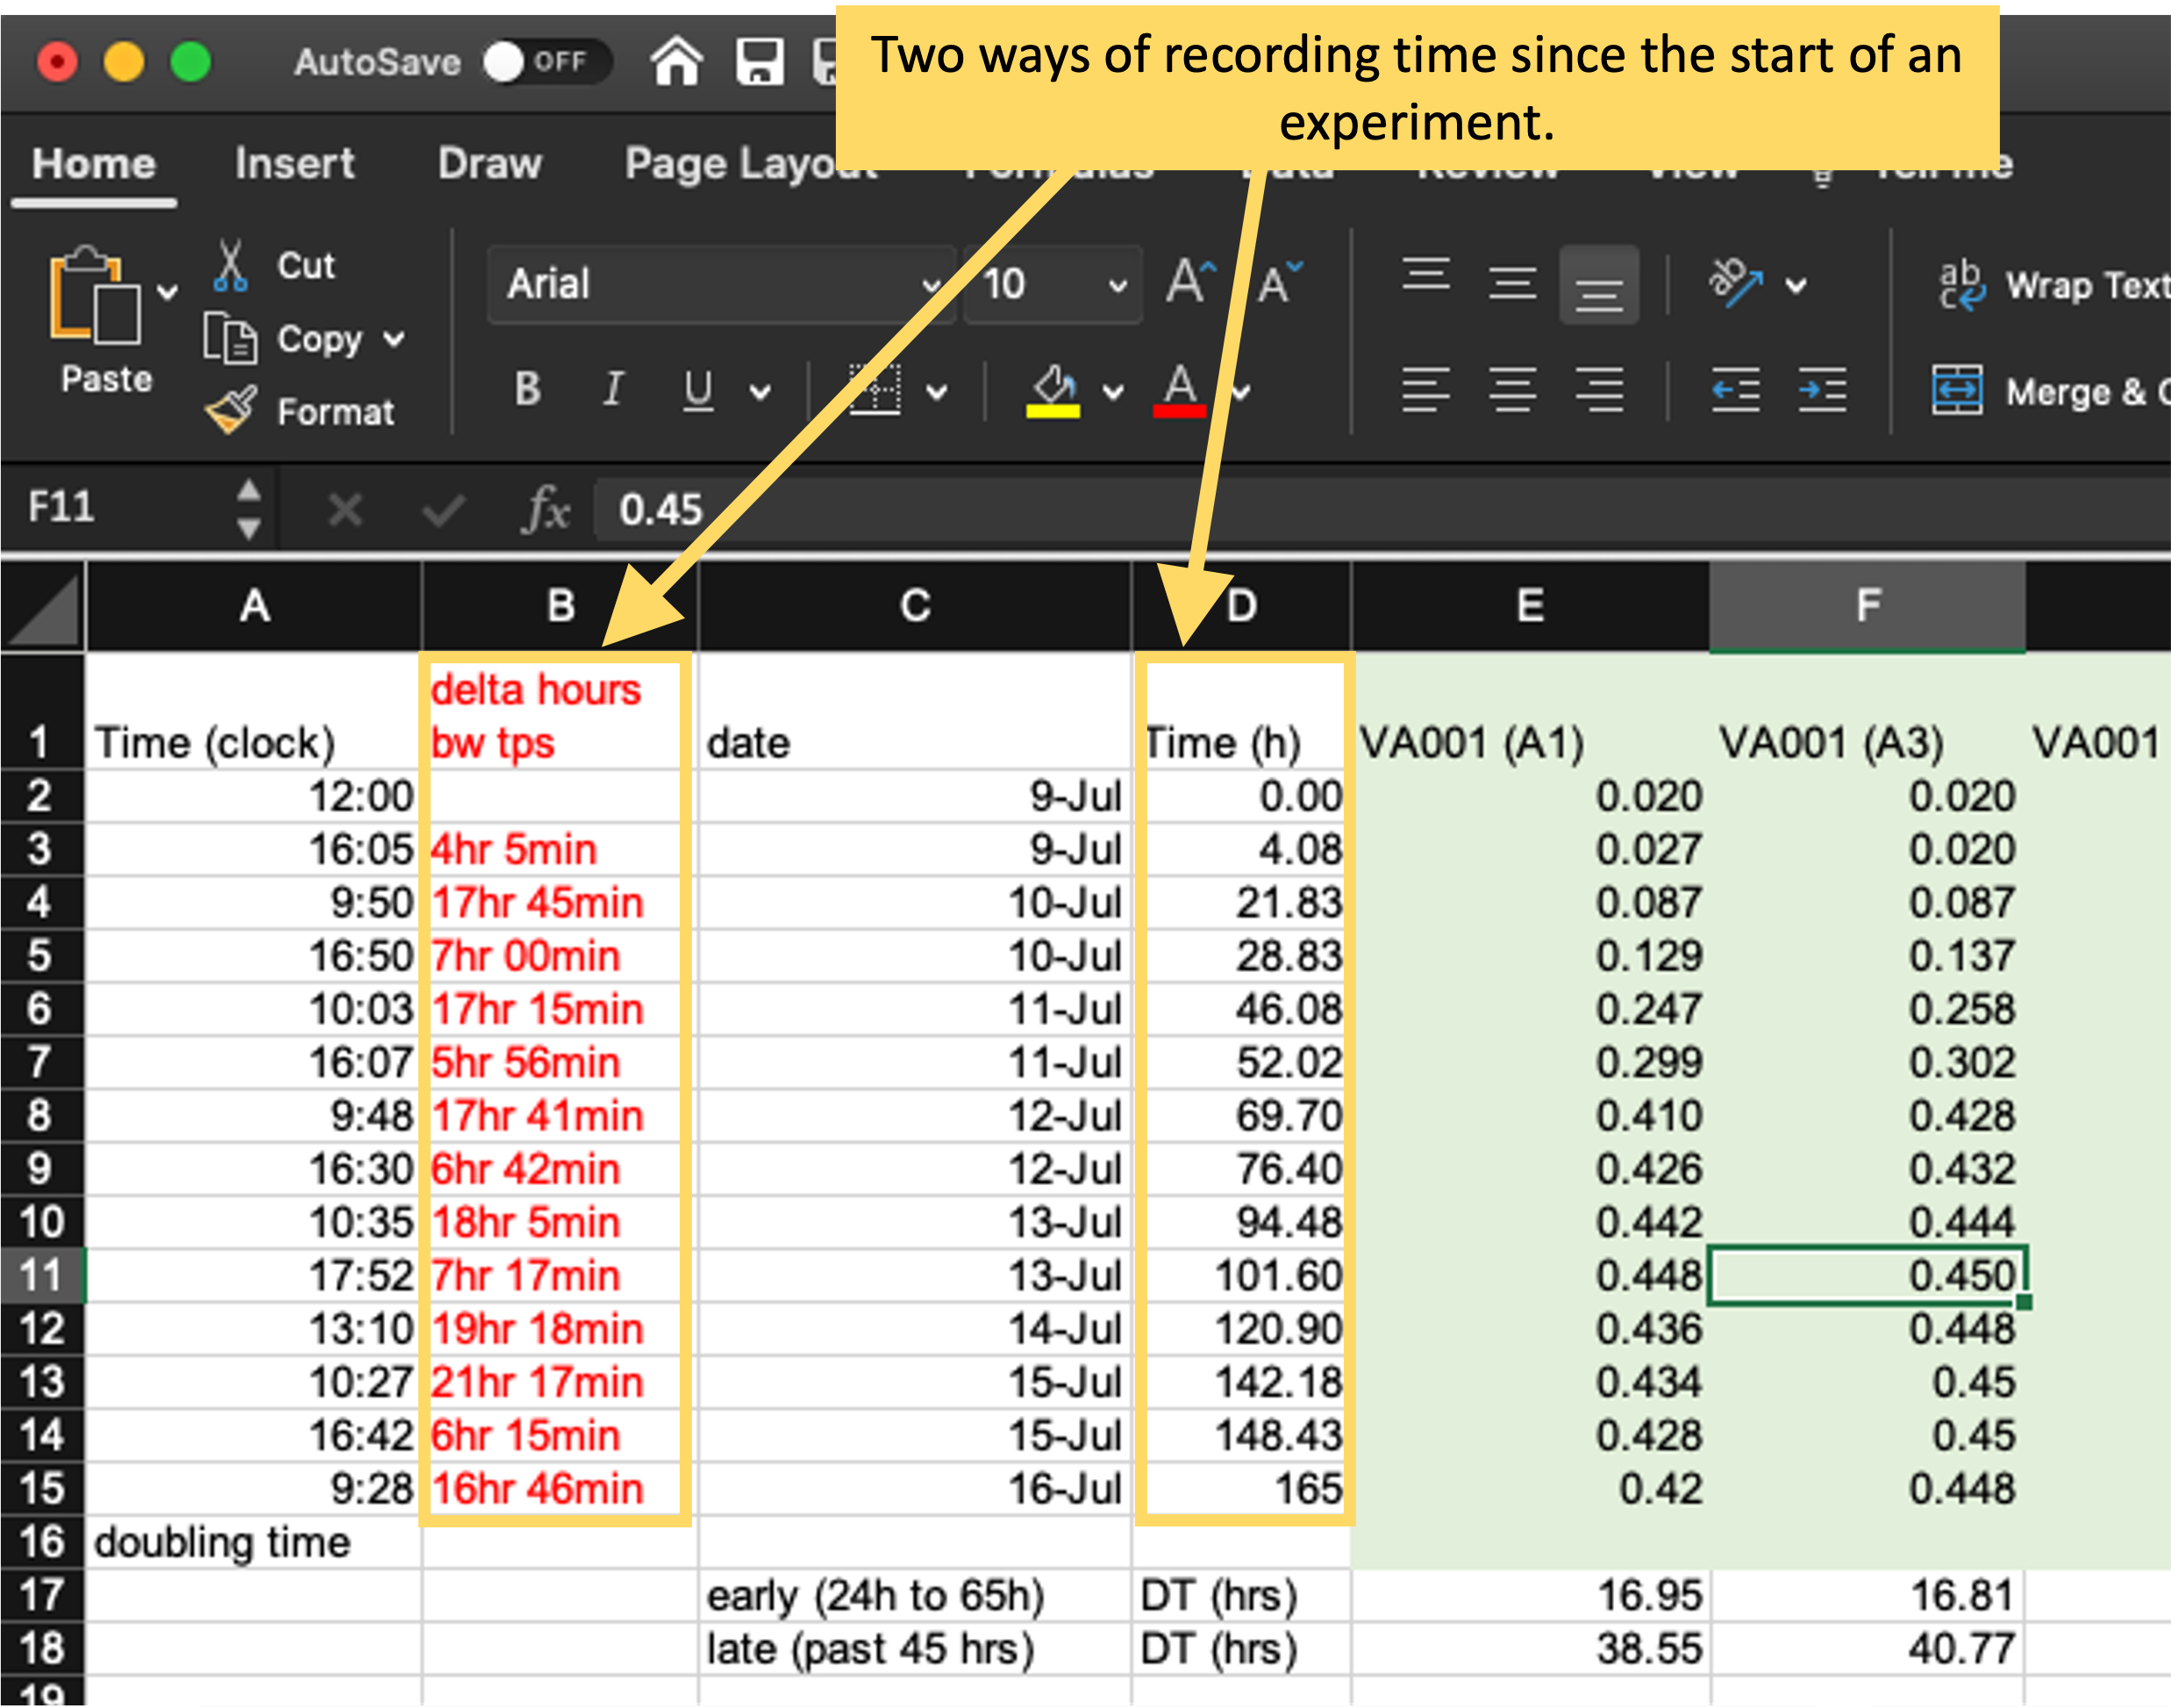
\includegraphics[width=\textwidth]{figures/growth_curve_recording_time} \caption[Examples of two ways of recording time in the original template from the example experiment]{Examples of two ways of recording time in the original template from the example experiment. Column B uses hours and minutes, with characters embedded to separate hours from minutes, while column D uses hours in decimal degrees. The format in column D will be much easier to integrate into a larger data analysis pipeline.}\label{fig:recordingtime}
\end{figure}

These three principles are an excellent starting point for designing a tidy
template for collecting data. By using these, you will be well on your way to
collecting data in a way that is easy to integrate in a longer reproducible data
analysis pipeline.

When you convert data collection templates to ``tidier'' formats, they will
typically look much simpler than the templates that your research group may have
been using. In the example experiment that we described earlier in this module,
this process of tidying the template results in a template like that shown in
Figure \ref{fig:growthsimple1} (in the next module, we'll walk through all the
steps to create this tidier template, using this principles we've covered in
this module). By comparison, the starting template for data collection for this
experiment is shown in Figure \ref{fig:growthexcel1}.

\begin{figure*}
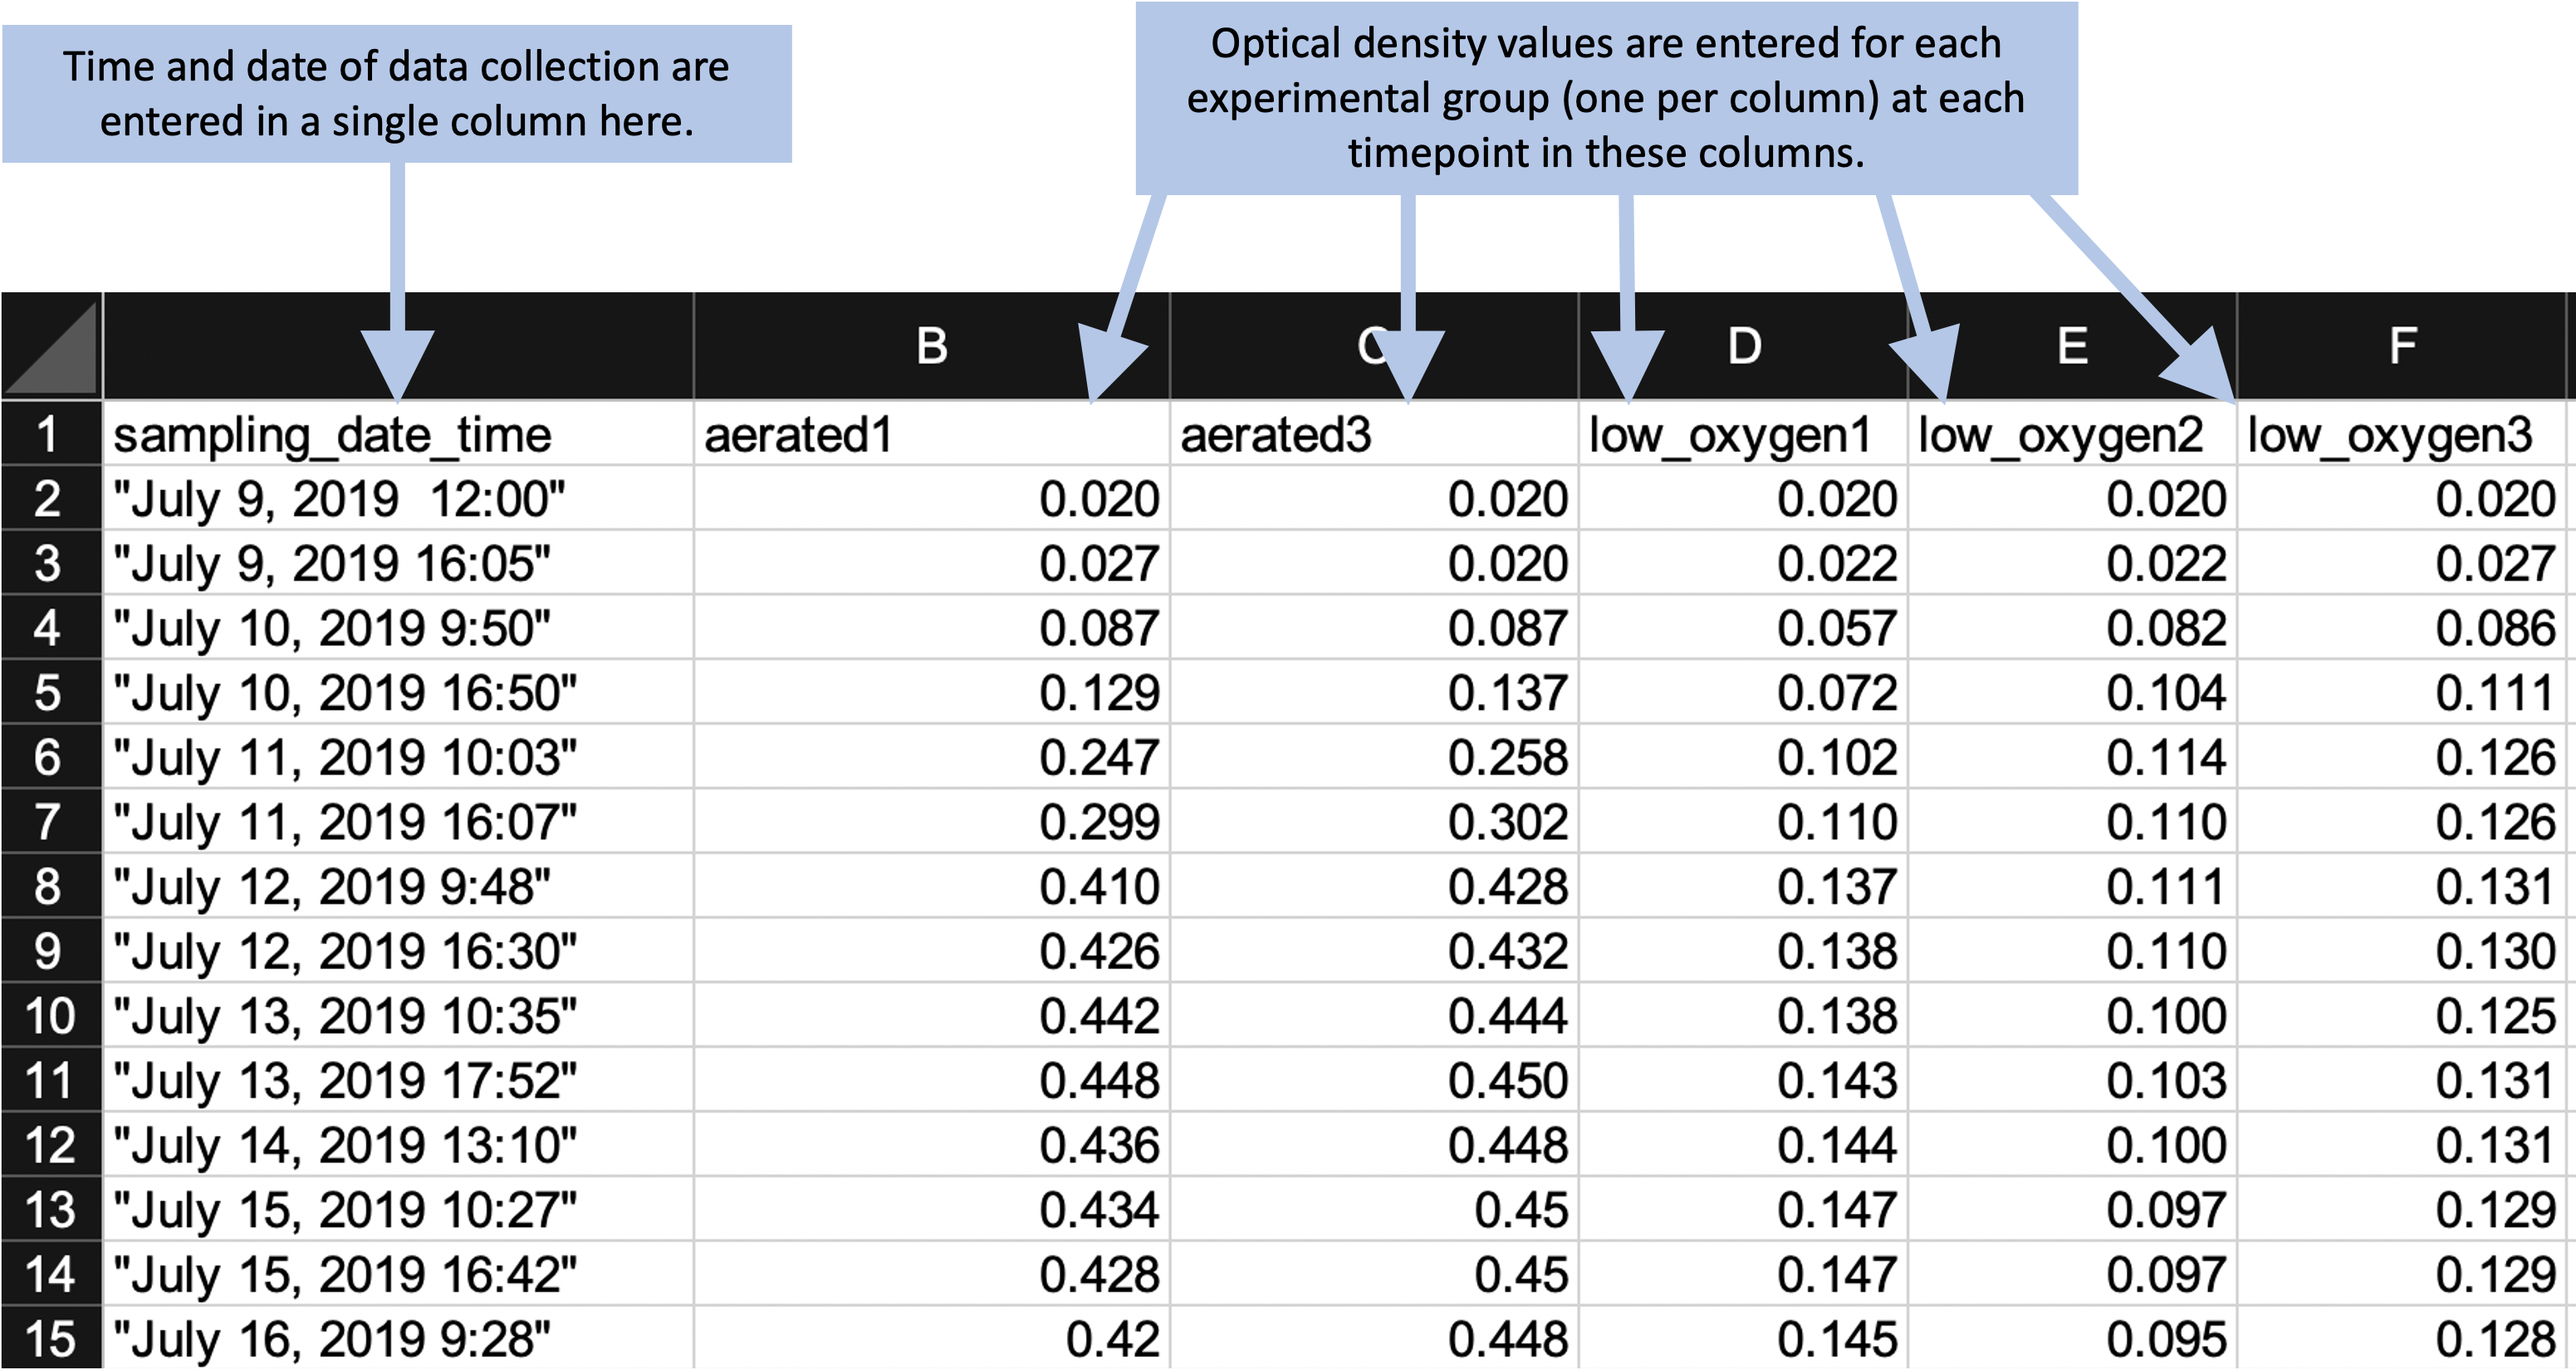
\includegraphics[width=\textwidth]{figures/growth_curve_simple} \caption[Example of an simpler format that can be used to record and analyze data for the same laboratory experiment as the previous figure]{Example of an simpler format that can be used to record and analyze data for the same laboratory experiment as the previous figure. Annotations highlight where data is entered by hand. No calculations are conducted or figures created---these are all done later, using a code script.}\label{fig:growthsimple1}
\end{figure*}

By comparing these two templates, you can see that the simpler template does
not, by itself, provide immediate, real-time summaries of the collected data. The
simpler template has removed elements like plots and values calculated by embedded
formulas. At first glance, this might seem like a disadvantage of using a tidier
template to collect data. However, by combining other tools in a pipeline, it is
easy to connect the tidier raw data file to reporting tools. In this way, you can
quickly create real-time summaries of the data that are similar to those shown in
Figure \ref{fig:growthexcel1}, but that are created and reported outside the file
used to originally record the data.

Figure \ref{fig:growthreport1} shows an example of a simple report that could
be created for the example experiment. This report is generated using a
statistical program, R, which inputs the data from the simple template shown in
Figure \ref{fig:growthsimple1}. The report then uses R code to generate a PDF
or Word file with the output shown below. The file for this report is created in
a way that the output can be quickly regenerated with a single button click, and
so it can be applied to other data saved using the same template. In fact, you can
create templates for reports that coordinate with each data collection template
that you create. In the next module, we'll walk through how you could create
the generating file for this report, and in later modules (3.7--3.9), we provide
a thorough overview of creating these types of ``knitted'' documents.

\begin{figure*}
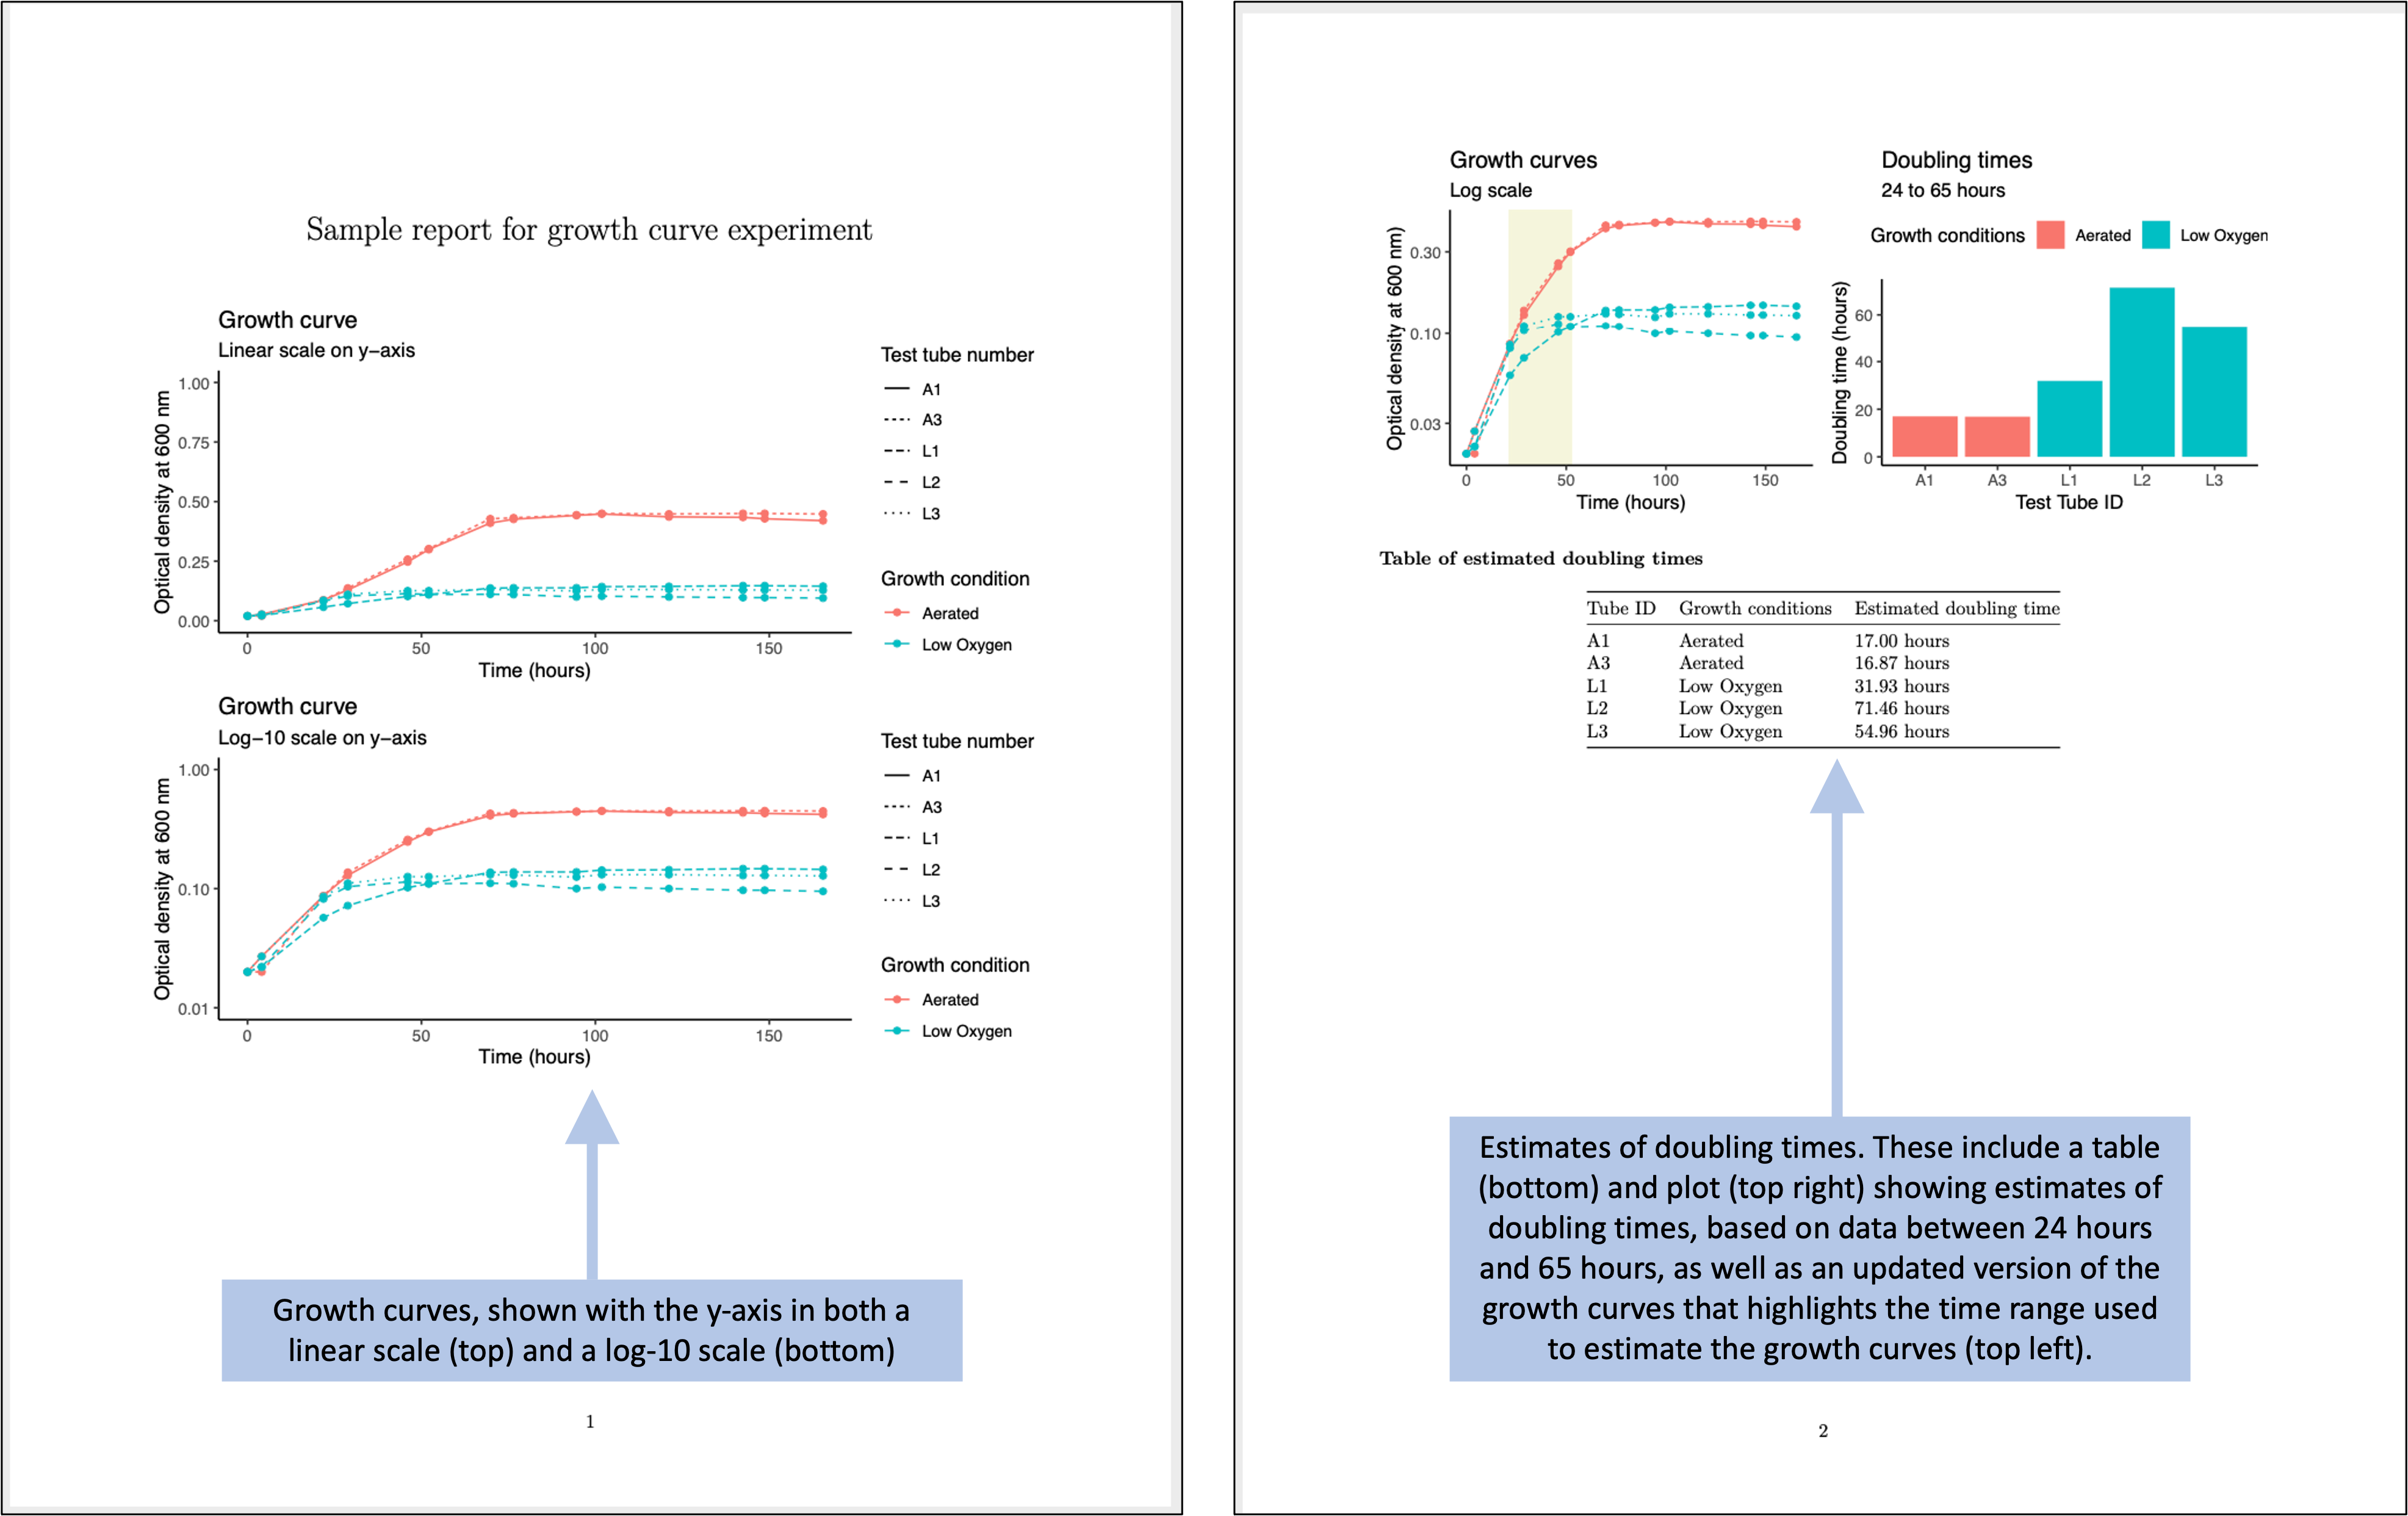
\includegraphics[width=\textwidth]{figures/growth_curve_report} \caption[Examples of an automated report that can be created to quickly generate summaries and estimates of the data collected in the simplified data collection template for the example experiment]{Examples of an automated report that can be created to quickly generate summaries and estimates of the data collected in the simplified data collection template for the example experiment.}\label{fig:growthreport1}
\end{figure*}

The report shown in Figure \ref{fig:growthreport1} repeats some of the same summaries
that were shown in the more complex original data collection template
(Figure \ref{fig:growthexcel1}). There are a number of advantages, however, to using
separate steps and files for the processes of collecting versus analyzing the data.
The separate report (Figure \ref{fig:growthreport1}) provides a starting point that can
be easily adapted to make more complex figures and analysis, as well as to integrate
the collected data with data measured in other ways for the experiment.

\subsection{Learning more about tidy data collection in the laboratory}\label{learning-more-about-tidy-data-collection-in-the-laboratory}

It may take some iteration to develop the data collection templates that are both
convenient and appropriate to input to more complex programs for pre-processing,
analysis, and visualization. This module and the next module provide guidance and
examples, but it can be helpful to see more examples. Two excellent resources on this
topic are articles by \citet{ellis2018share} and \citet{broman2018data}.

\section{Example: Creating a template for ``tidy'' data collection}\label{module5}

We will walk through an example of creating a template to collect data in a
``tidy'' format for a laboratory-based research project, based on a research
project on drug efficacy in murine tuberculosis models. It is important to note
that there's no reason that you can't continue to use a spreadsheet program like
Excel or Google Sheets to collect data. The spreadsheet program itself can
easily be used to create a simple template to use as you collect data. In fact,
we'll continue using a spreadsheet format in this module as we show how to
redesign the data collection for the example experiment that we introduced in
the last module. It is important, however, to think through how you will arrange
that template spreadsheet to make it most useful in the larger context of
reproducible research.

As we show how to redesign the data collection template, we'll focus on the
three principles for designing tidy templates for data collection in a
biomedical laboratory that we introduced in module 2.4. As a reminder, those
three principles are:

\begin{enumerate}
\def\labelenumi{\arabic{enumi}.}
\tightlist
\item
  Limit the template to the collection of data.
\item
  Make sensible choices when dividing data collection into rows and columns.
\item
  Avoid characters or formatting that will make it hard for a computer program
  to process the data.
\end{enumerate}

In this module, we'll show you how to apply those principles to create a tidier
template for the example dataset from the last module. Finally, we will show how
the data can then easily be analyzed and visualized using reproducible tools.

\textbf{Objectives.} After this module, the trainee will be able to:

\begin{itemize}
\tightlist
\item
  Understand how the principles of ``tidy'' data can be applied for a real, complex research project
\item
  List advantages of the ``tidy'' data format for the example project
\item
  Apply steps that follow three principles for creating a template for ``tidy''
  data collection
\item
  Construct a template for ``tidy'' data collection
\item
  Explain how a report template can help replace visualization tools in a
  spreadsheet when collecting data
\end{itemize}

\subsection{Example data---Data on rate of bacterial growth}\label{example-datadata-on-rate-of-bacterial-growth}

Here, we'll walk through an example using real data collected in a laboratory
experiment. We described these data in detail in the previous module. As a
reminder, they were collected to measure the growth rate of \emph{Mycobacteria
tuberculosis} under two conditions---high oxygen and low oxygen. They were
collected from five test tubes that were measured regularly over one week for
bacteria growth using a measure of optical density. Figure
\ref{fig:growthexcel2} shows the original template that the research group used
to record these data.

\begin{figure*}
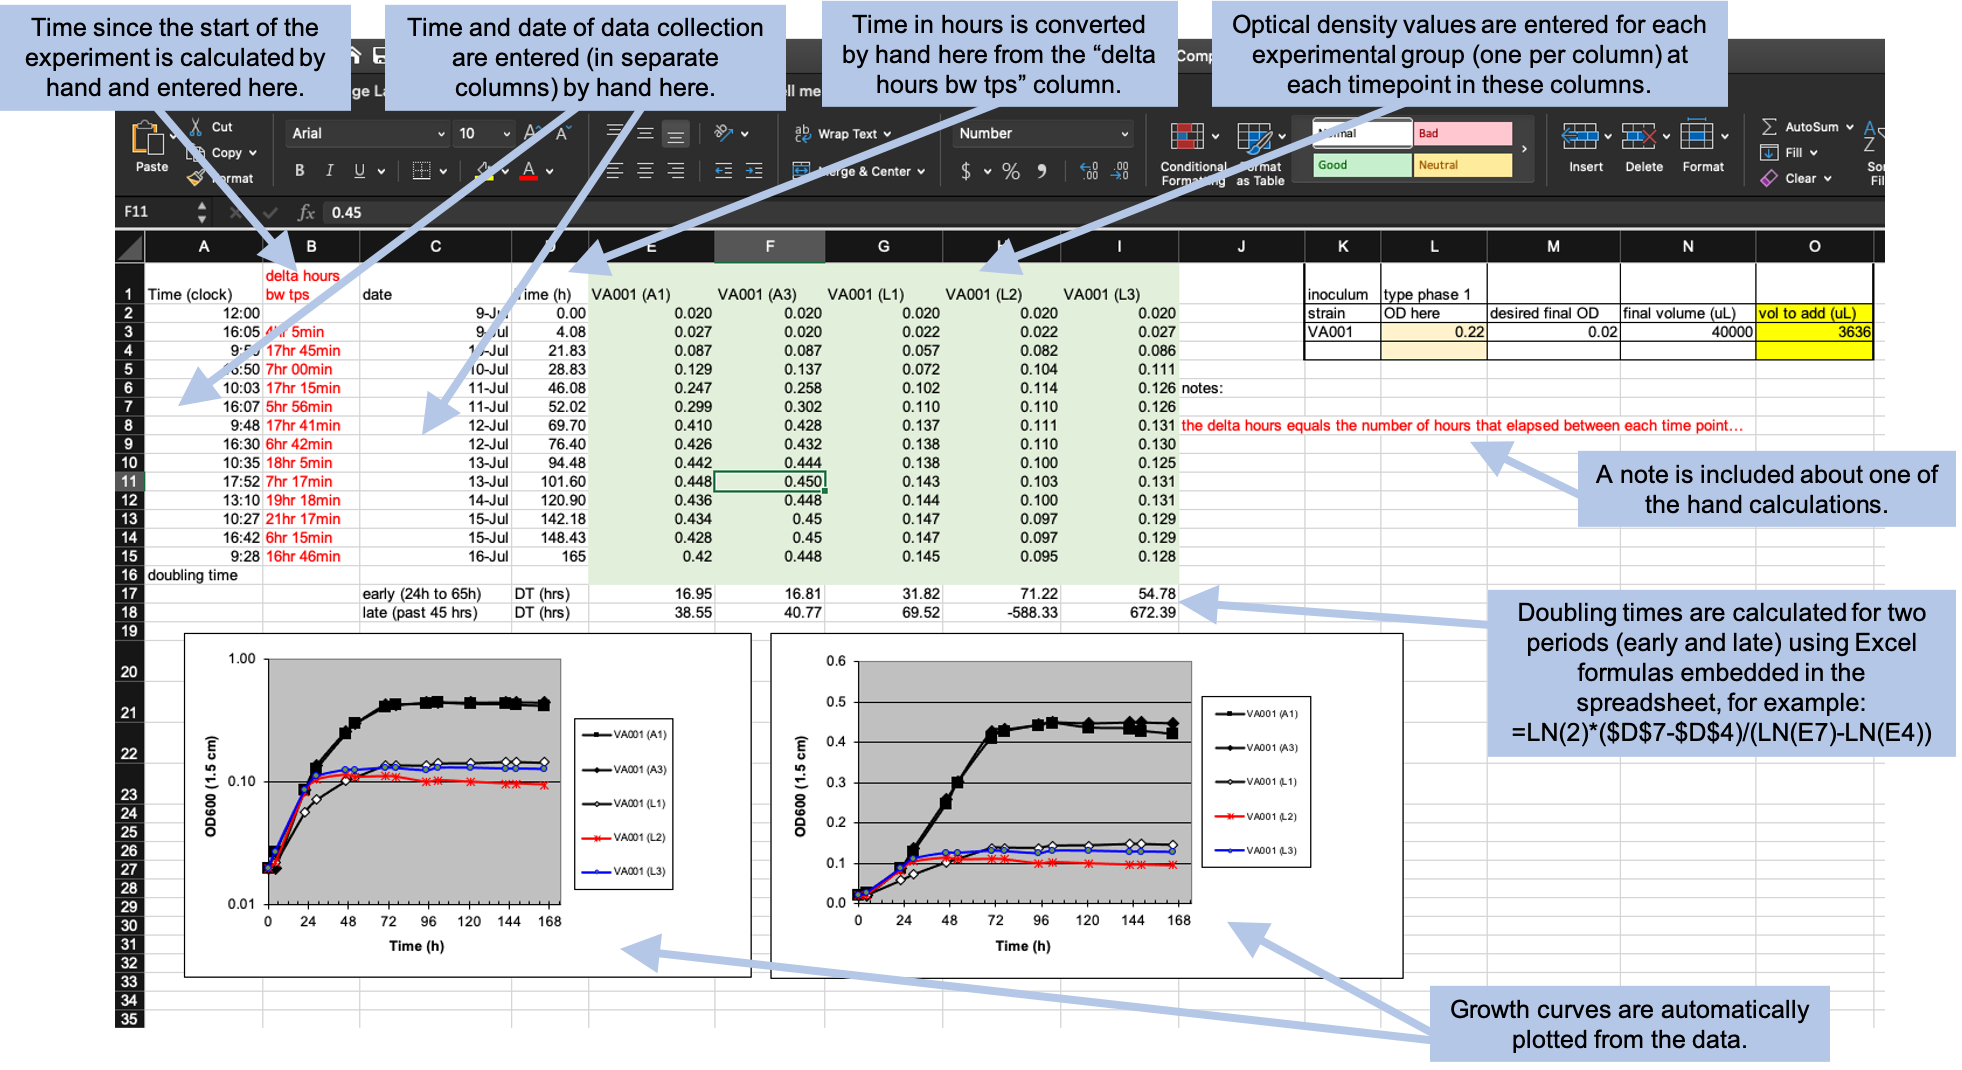
\includegraphics[width=\textwidth]{figures/growth_curve_example} \caption[Example of an Excel spreadsheet used to record and analyze data for a laboratory experiment]{Example of an Excel spreadsheet used to record and analyze data for a laboratory experiment. Annotations highlight where data is entered by hand, where calculations are done by hand, and where embedded Excel formulas are used. The figures are created automatically using values in a specified column.}\label{fig:growthexcel2}
\end{figure*}

In the previous module, we described features that make this template ``untidy''
and potentially problematic to include in a larger pipeline of reproducible
research. In the next few sections of this module, we'll walk step-by-step
through changes that you could make to make this template tidier. We'll finish
the module by showing how you could then design a further step of the
analysis pipeline to visualize and analyze the collected data, so that the
advantages of real-time plotting from the more complex spreadsheet are not
missed when moving to a tidier template.

\subsection{Limiting the template to the collection of data}\label{limiting-the-template-to-the-collection-of-data}

The first principle in designing a template for tidy data collection is to
\textbf{limit the template to the collection of data.} The example template (Figure
\ref{fig:growthexcel2}), however, includes a number of ``extra'' elements beyond
simple data collection---all the elements outside rows 1--15 of columns A--I.
Outside this area, there are a number of extra elements, including plots that
visualize the data, summaries generated based on the data (rows 16--18, for
example), notes about the data, and even a macro (top right) that wasn't
involved in data collection but instead was used by the researcher to calculate
the initial volume of inoculum to include in each test tube. None of these
``extras'' can be easily read into a statistical program like R or Python---at
best, they will be ignored by the program. They can even complicate reading in
the cells with measurements (rows 1--15 of columns A--I), as most statistical
programs will try to read in all the non-empty cells of a spreadsheet unless
directed otherwise.

A good starting point, then, would be to start designing a tidy data collection
template for this experiment by extracting only the content from the box in
Figure \ref{fig:extractraw}. This would result in a template that looks like
Figure \ref{fig:step1}. Notice that, as we've done this, we've also removed any
of the color formatting from the spreadsheet. It is fine to keep color in the
spreadsheet if it will help the research to find the right spot to record data
while working in the laboratory, but you should make sure that you're not using
it to encode information about the data---all color formatting will be ignored
when the data are read by a statistical program like R.

\begin{figure*}
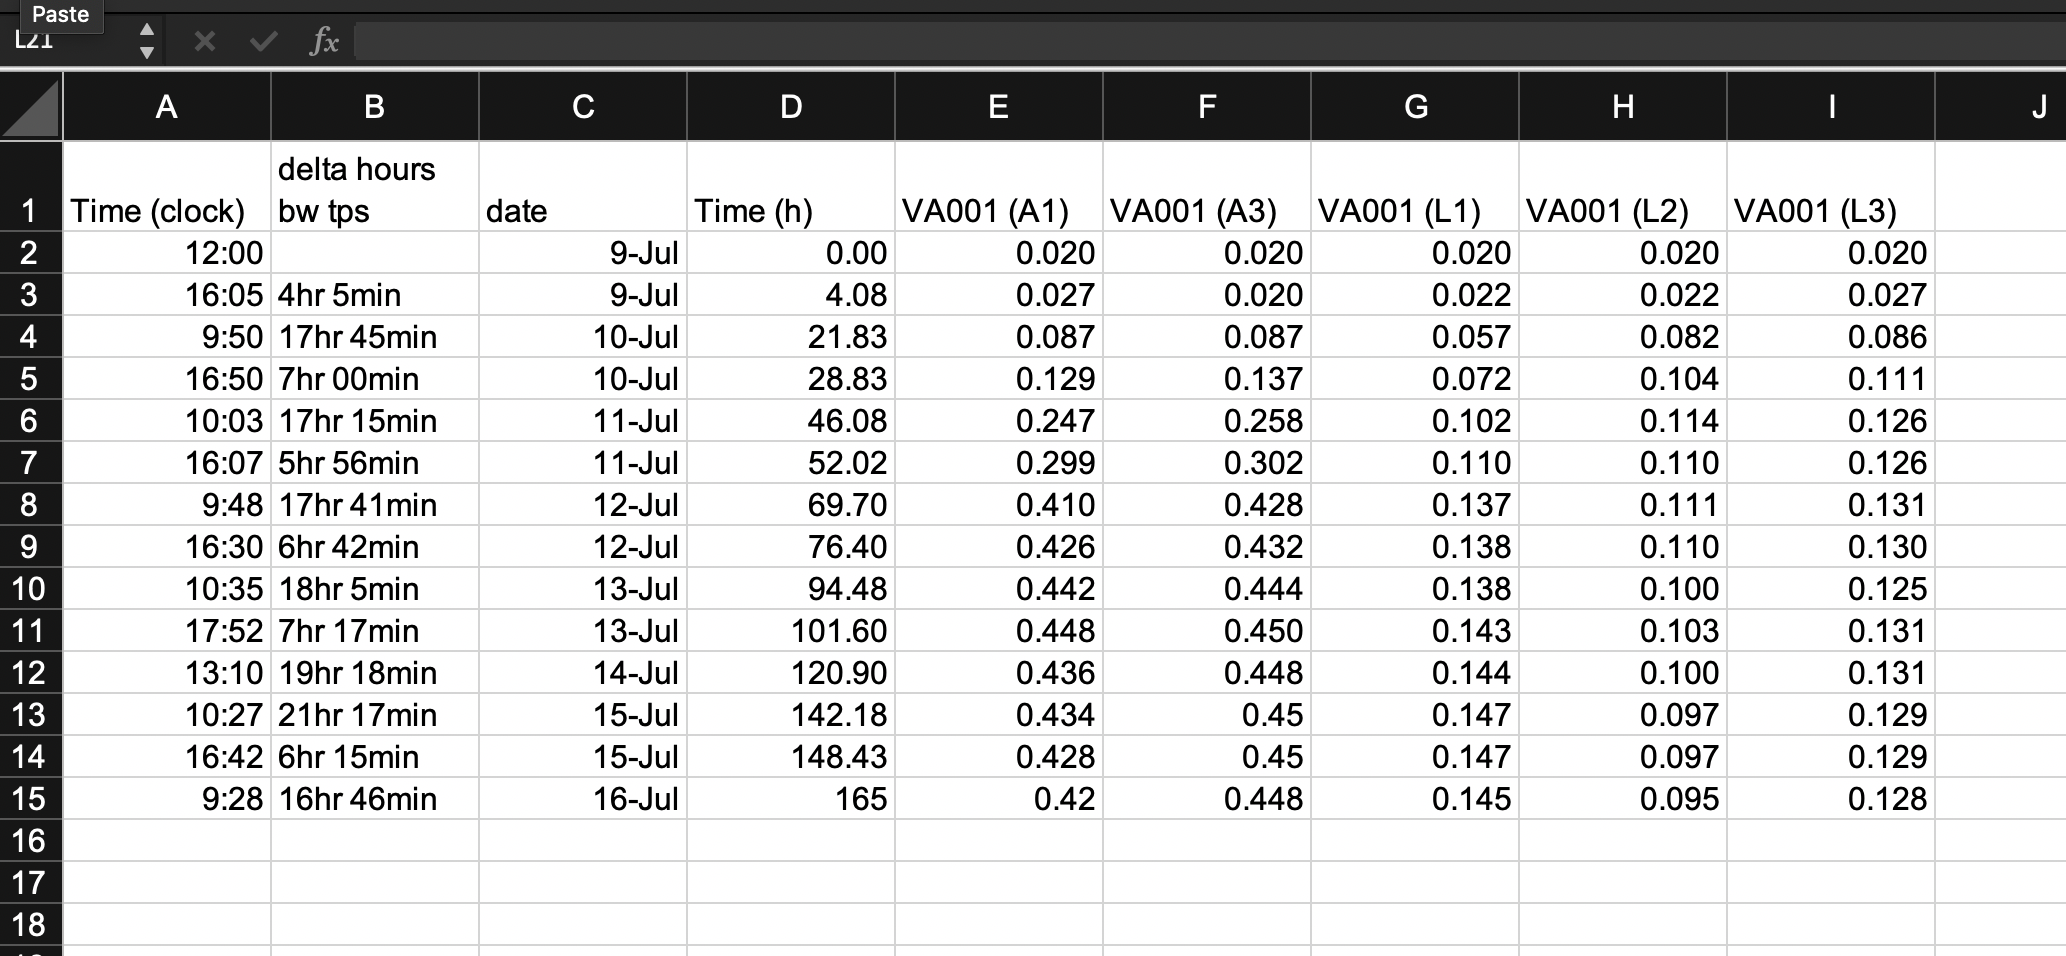
\includegraphics[width=\textwidth]{figures/growth_curve_step1} \caption[First step in designing a tidy data collection template for the example project]{First step in designing a tidy data collection template for the example project. A template has been created that focuses only on the raw data, removing all extra elements like plots, notes, macros, and summaries.}\label{fig:step1}
\end{figure*}

Other ``extras'' in spreadsheets are embedded elements like formulas and macros.
To make your data collection tidy, you should remove any computation steps from
the file that you use to record the data. While the template shown in Figure
\ref{fig:step1} has removed a lot of the calculated values from the original
template, it has not removed all of them. Two of the columns are still values
that were determined by calculation after the original data were collected.
Column B and column D both provide measures of the length of time since the
start of the experiment, and both are calculated by comparing a measurement time
to the time at the start of the experiment.

The time since the start of the experiment can easily be calculated later in the
analysis pipeline, once you read the data into a statistical program like R. By
delaying this step, you can both simplify the data collection template
(requiring fewer columns for the research in the laboratory to fill out) and
also avoid the chance for mistakes, which could occur both in the hand
calculations of these values and in data entry, when the researcher enters the
results of the calculations in the spreadsheet cell. Figure \ref{fig:step2}
shows a new version of the template, where these calculated columns have been
removed. This template is now restricted to only data points originally
collected in the course of the experiment. It has removed all elements that are
based on calculations or other derivatives of those original, raw data points.

\begin{figure}
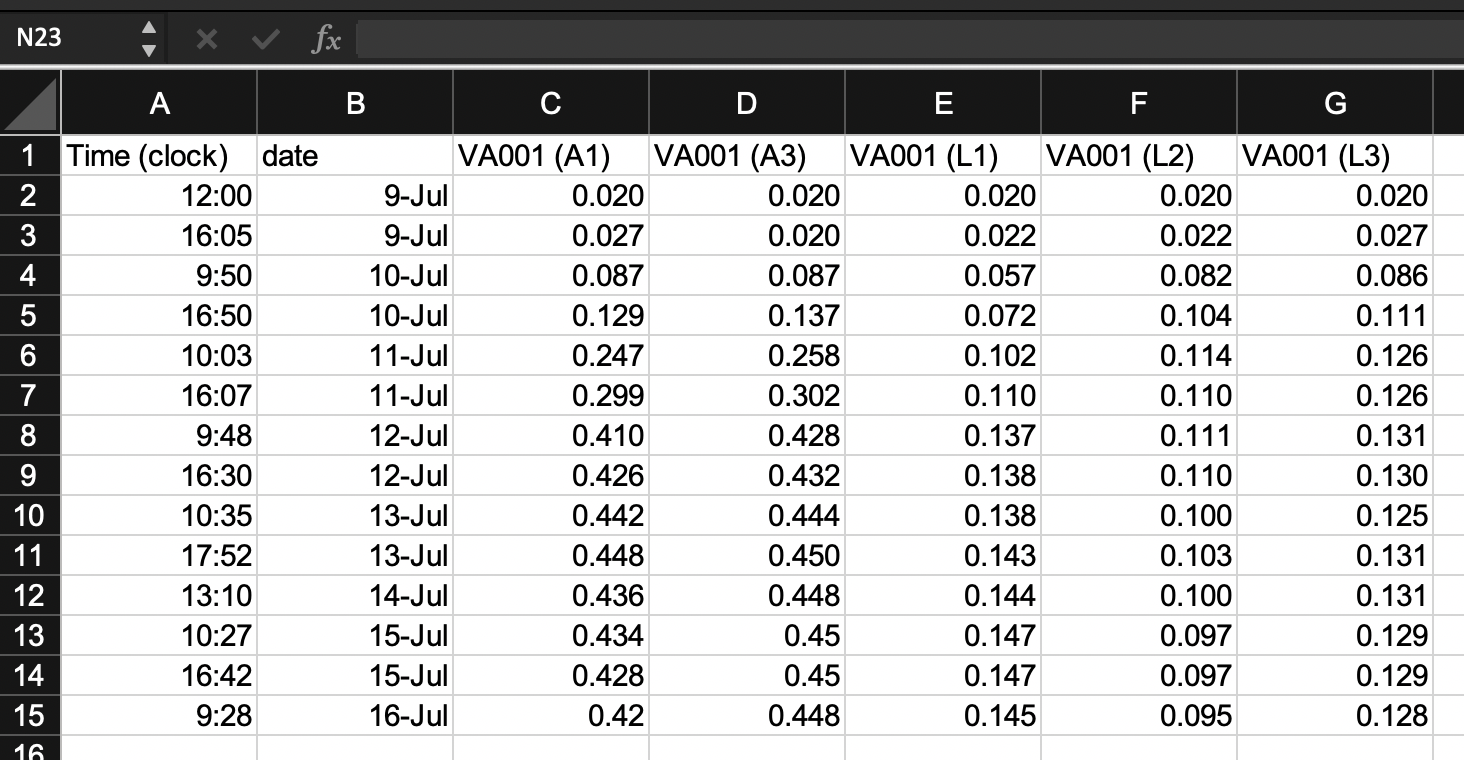
\includegraphics[width=\textwidth]{figures/growth_curve_step2} \caption[Second step in designing a tidy data collection template for the example project]{Second step in designing a tidy data collection template for the example project. This template started from the previous one, but removed columns that were hand-calculated and then entered by the researcher in the previous template. This version has removed all calculated values on the template, limiting it to only the original recorded values required for the experiment.}\label{fig:step2}
\end{figure}

\subsection{Making sensible choices about rows and columns}\label{making-sensible-choices-about-rows-and-columns}

The second principle in designing a template for tidy data collection is to
\textbf{make sensible choices when dividing data collection into rows and columns}.
There are many different ways that you could spread the data collection into
rows and columns, and in this step, you can consider which method would meet a
reasonable balance between making the template easy for the researcher in the
laboratory to use to record data and also making the resulting data file easy to
incorporate in a reproducible data analysis pipeline.

For the example experiment, Figure \ref{fig:extractraw} shows three possibilities
that we can consider to arrange data collection across rows and columns.
All three build on the changes we made in the earlier step of ``tidying'' the template,
which resulted in the template shown in Figure \ref{fig:step2}.

\begin{figure*}
\includegraphics[width=\textwidth]{figures/growth_curve_column_options} \caption[Examples of ways that data collection could be divided into rows and columns in the example template]{Examples of ways that data collection could be divided into rows and columns in the example template. Panel A shows an example where date and time are recorded in different columns. Panel B is similar to Panel A, but in this case, date and time are recorded in a single column. Panel C shows a classically 'tidy' data format, where each measurement date-time is repeated for each of the five test tubes, and columns give the test tube ID and absorbance measurement at that time for that tube (only part of the data is shown for this format, while remaining rows are off the page). While Panel C provides the 'tidiest' format, it may have some practical constraints when used in a laboratory setting. For example, it would require more data entry during data collection (since date-time is entered five times at each measurement time), and its long format prevent it all from being seen at once without scrolling on a computer screen.}\label{fig:columnoptions}
\end{figure*}

Panel A (an exact repeat of the template shown in Figure \ref{fig:step2}) shows
an example where date and time are recorded in different columns. Panel B is
similar to Panel A, but in this case, date and time are recorded in a single
column. Panel C shows a classically ``tidy'' data format, where each measurement's
date-time is repeated for each of the five test tubes, and columns give the test
tube ID and absorbance measurement at that time for that tube (only part of the
data is shown for this format, while remaining rows are off the page).

In this example, the template that may be the most reasonable is the one shown
in Panel B. While Panel C provides the ``tidiest'' format (module 2.3), it has
some practical constraints when used in a laboratory setting. For example, it
would require more data entry during data collection (since date-time is entered
five times at each measurement time), and its long format prevent it all from
being seen at once without scrolling on a computer screen.

When comparing Panels A and B, the template in Panel B has an advantage. The
information on date and time are useful together, but not individually. For
example, to calculate the time since the start of the experiment, you cannot
just calculate the difference in dates or just the difference in times, but
instead must consider both the date and time of the measurement in comparison to
the date and time of the start of the experiment. As a result, at some point in
the data analysis pipeline, you'll need to combine information about the date
and the time to make use of the two elements.

While this combination of two columns can be easily done within a statistical
program like R, it can also be directly designed into the original template for
collecting the data. Therefore, unless there is a practical reason why it would
be easier for the researcher to enter date and time separately, the template
shown in Panel B is preferable to that shown in Panel A in terms of allowing for
the ``tidy'' collection of research data into a file that is easy to include in a
reproducible pipeline.

Figure \ref{fig:step3} shows the template design at this stage in the process
of tidying it, highlighting the column that combines date and time elements in a
single column. In this version of the template, we've also been careful about
how date and time are recorded, a consideration that we'll discuss more in the
next section.

\begin{figure*}
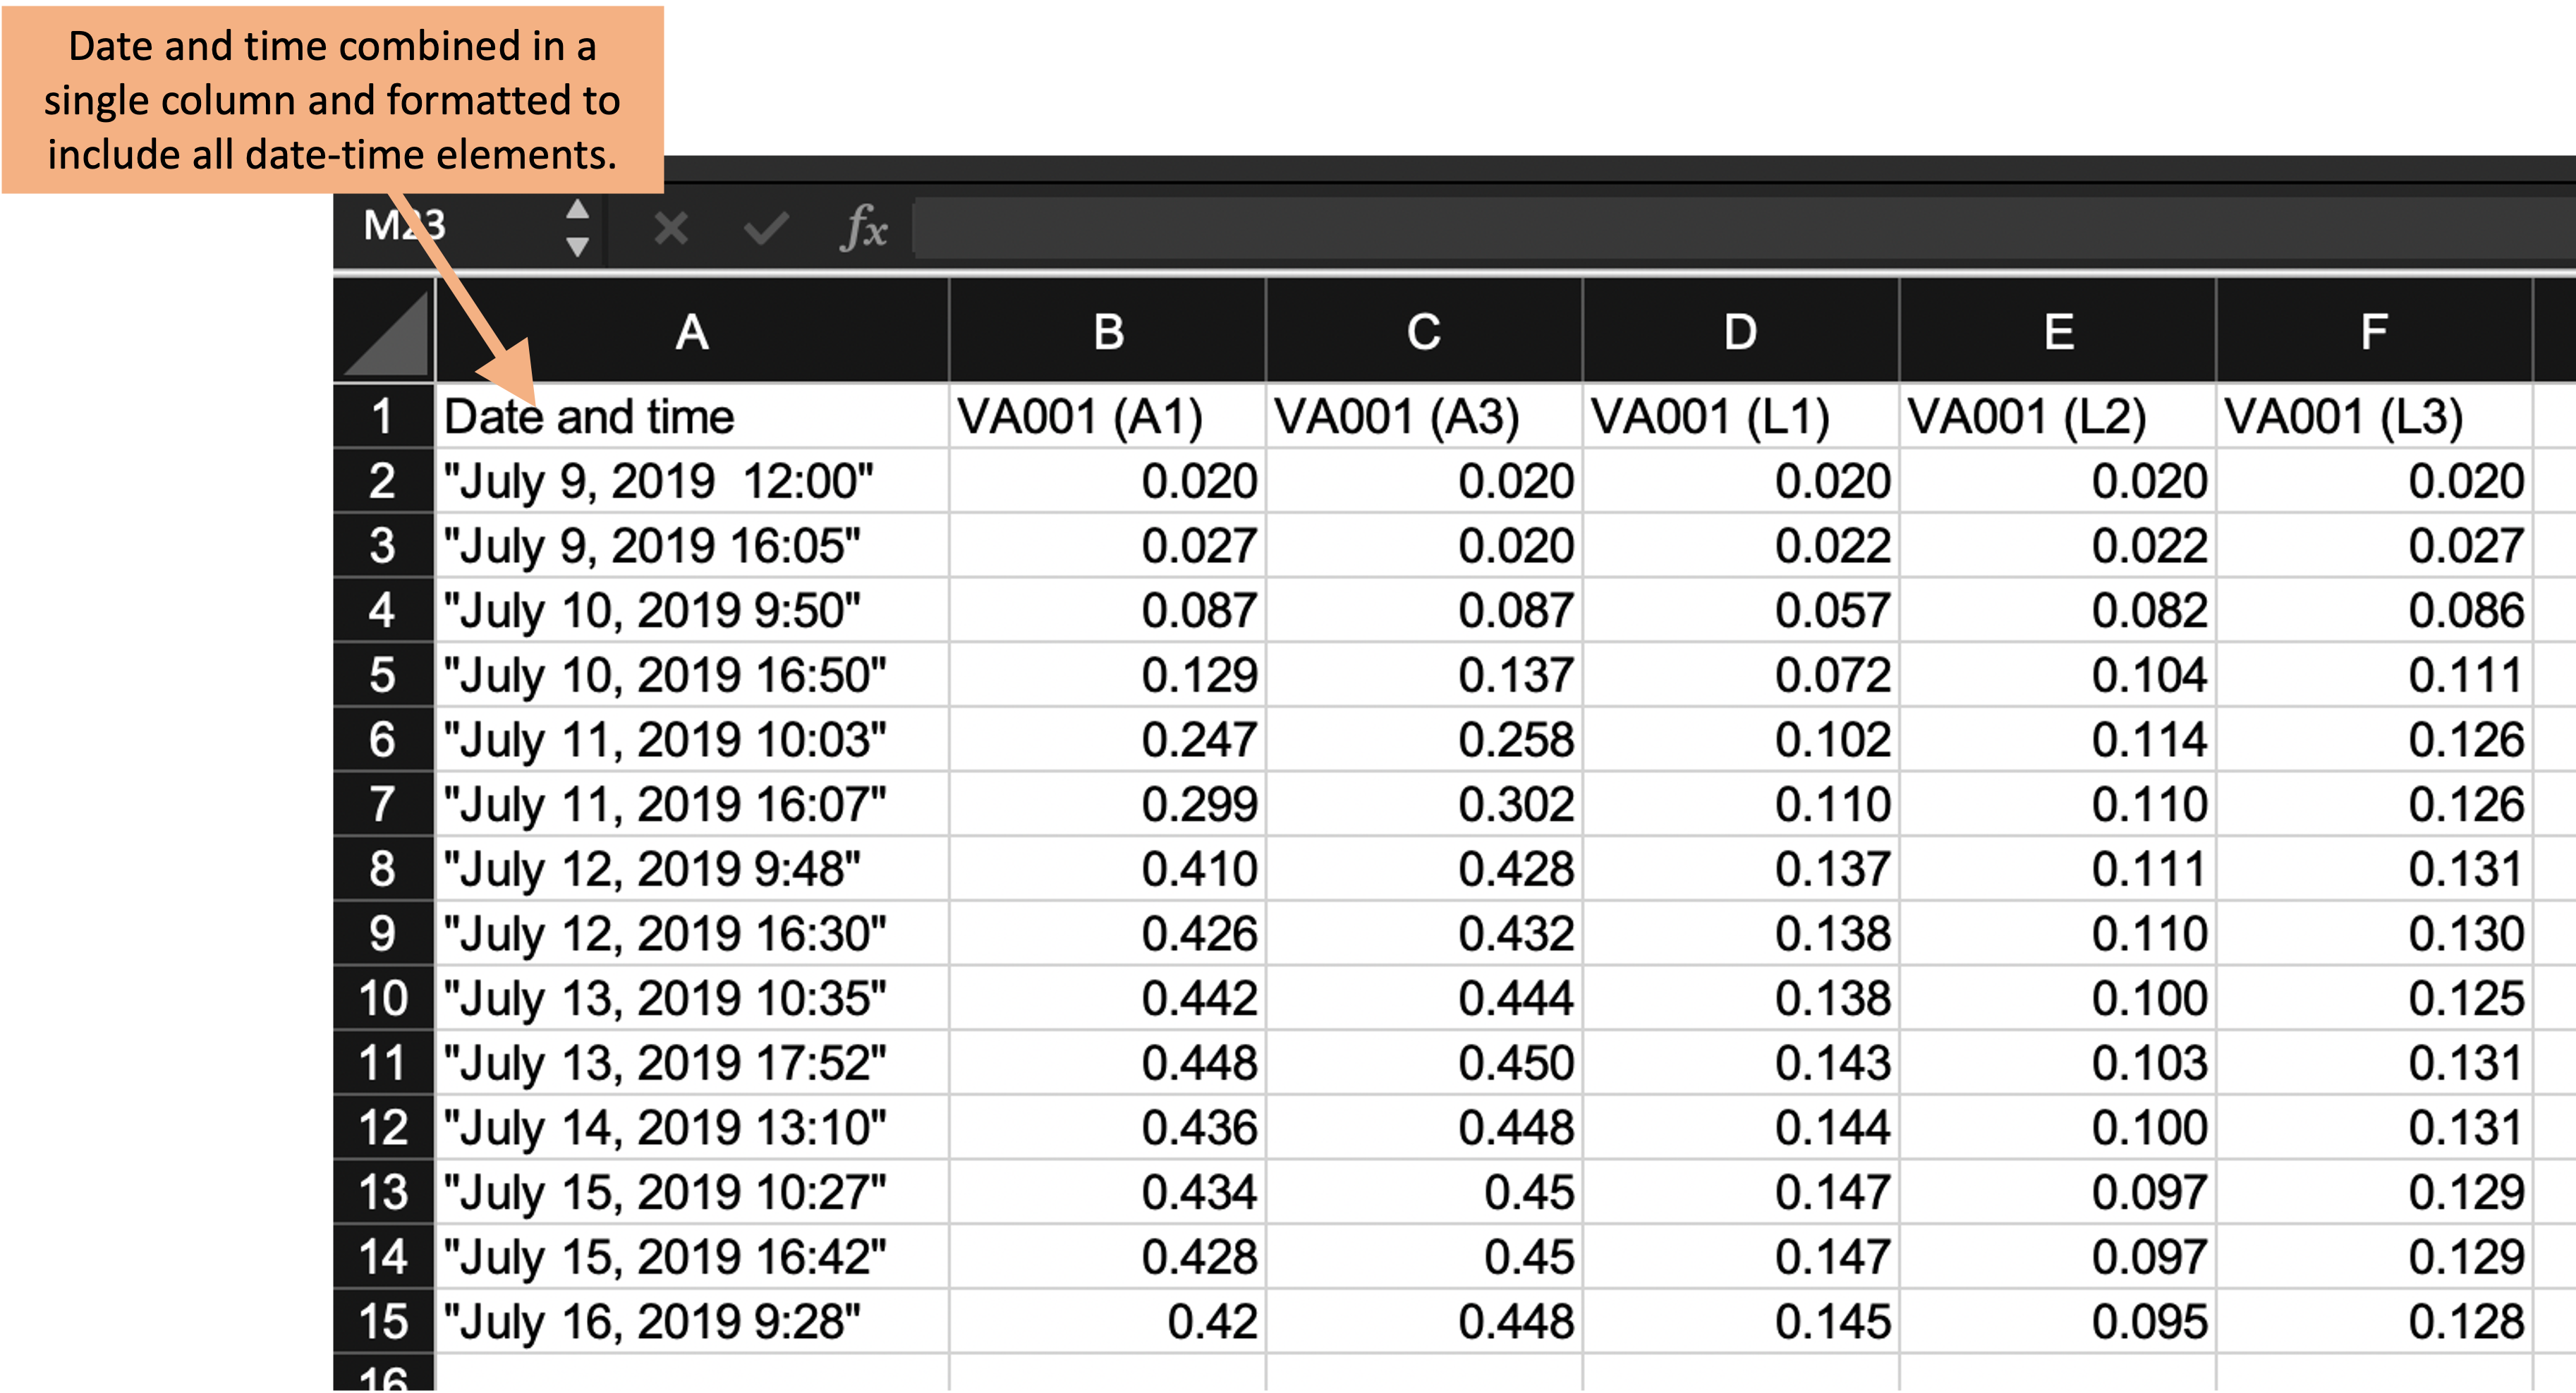
\includegraphics[width=\textwidth]{figures/growth_curve_step3} \caption[Third step in designing a tidy data collection template for the example project]{Third step in designing a tidy data collection template for the example project. This template started from the previous one, but combined collection of the date and time of the measurement into a single column and revised the format to include all date elements and to prevent automatic conversion by the spreadsheet program.}\label{fig:step3}
\end{figure*}

\subsection{Avoiding problematic characters or formatting}\label{avoiding-problematic-characters-or-formatting}

The third principle in designing templates for tidy data collection is to
\textbf{avoid characters or formatting that will make it hard for a computer program
to process the data}. There are a number of special characters and formatting
conventions that can be hard for a statistical program to handle. In the example
template shown in Figure \ref{fig:step3}, for example, the column names include
spaces (for example, in ``Date and time''), as well as parentheses (for example,
in ``VA 001 (A1)''). While most statistical programs have tools that allow you to
handle and convert these characters once the data are read in, it's even simpler
to choose column names that avoid these problems in the original data collection
template. This will save some extra coding further along in the analysis
pipeline. Two general rules for creating easy-to-use column names in a data
collection template are: (1) start each column name with a letter and (2) for
the rest of the column name, use only letters, numbers, or the underscore
character (``\_``). For example,''aerated1'' would work well, but ``1--aerated'' of
``aerated--1'' would not.

Within the cell values below the column names, there is more flexibility. For
example, if you have a column that gives the IDs of different samples, it would
be fine to include spaces and other characters in those IDs. There are a few
exceptions, however. A big one is with values that record dates or date-time
combinations.

First, it is important to include all elements of the date (or date and time, if
both are recorded). The year should be included in the recorded
date, even if the experiment only took a few days. This is because statistical
programs have excellent functions for working with data that are dates or
date-times, but to take advantage of these, the data must be converted into a
special class in the program, and conversion to that class requires specific
elements (for a date, it must include the year, month, and day of month).

Second, it is useful to avoid recording dates and date-times in a way that
results in a spreadsheet program automatically converting them. Surrounding the
information about a date in quotation marks when entering it (as shown in Figure
\ref{fig:step3}) can avoid this.

Finally, consider using a format to record the date that is unambiguous and so
less likely to have recording errors. Dates are sometimes recorded using only
numbers---for example, the first date of ``July 9, 2019'' in the example data
could be recorded as ``7/9/2019'' or ``7/9/19'', to be even more concise. However,
this format has ambiguity. It can be unclear if this refers to July 9 or to
September 7, both of which could be written as ``7/9''. For the version that uses
two digits for the year, it can be unclear if the date is for 2019 or 1919 (or
any other century). Using the format ``July 9, 2019'', as done in the latest
version of the sample template, avoids this potential ambiguity.

Figure \ref{fig:growthsimple2} shows the template for the example experiment after the
column names have been revised to avoid any problematic characters. This template is now in
a very useful format for a reproducible research pipeline---the data collected using this
template can be very easily read into and processed using further statistical programs like
R or Python.

\begin{figure}
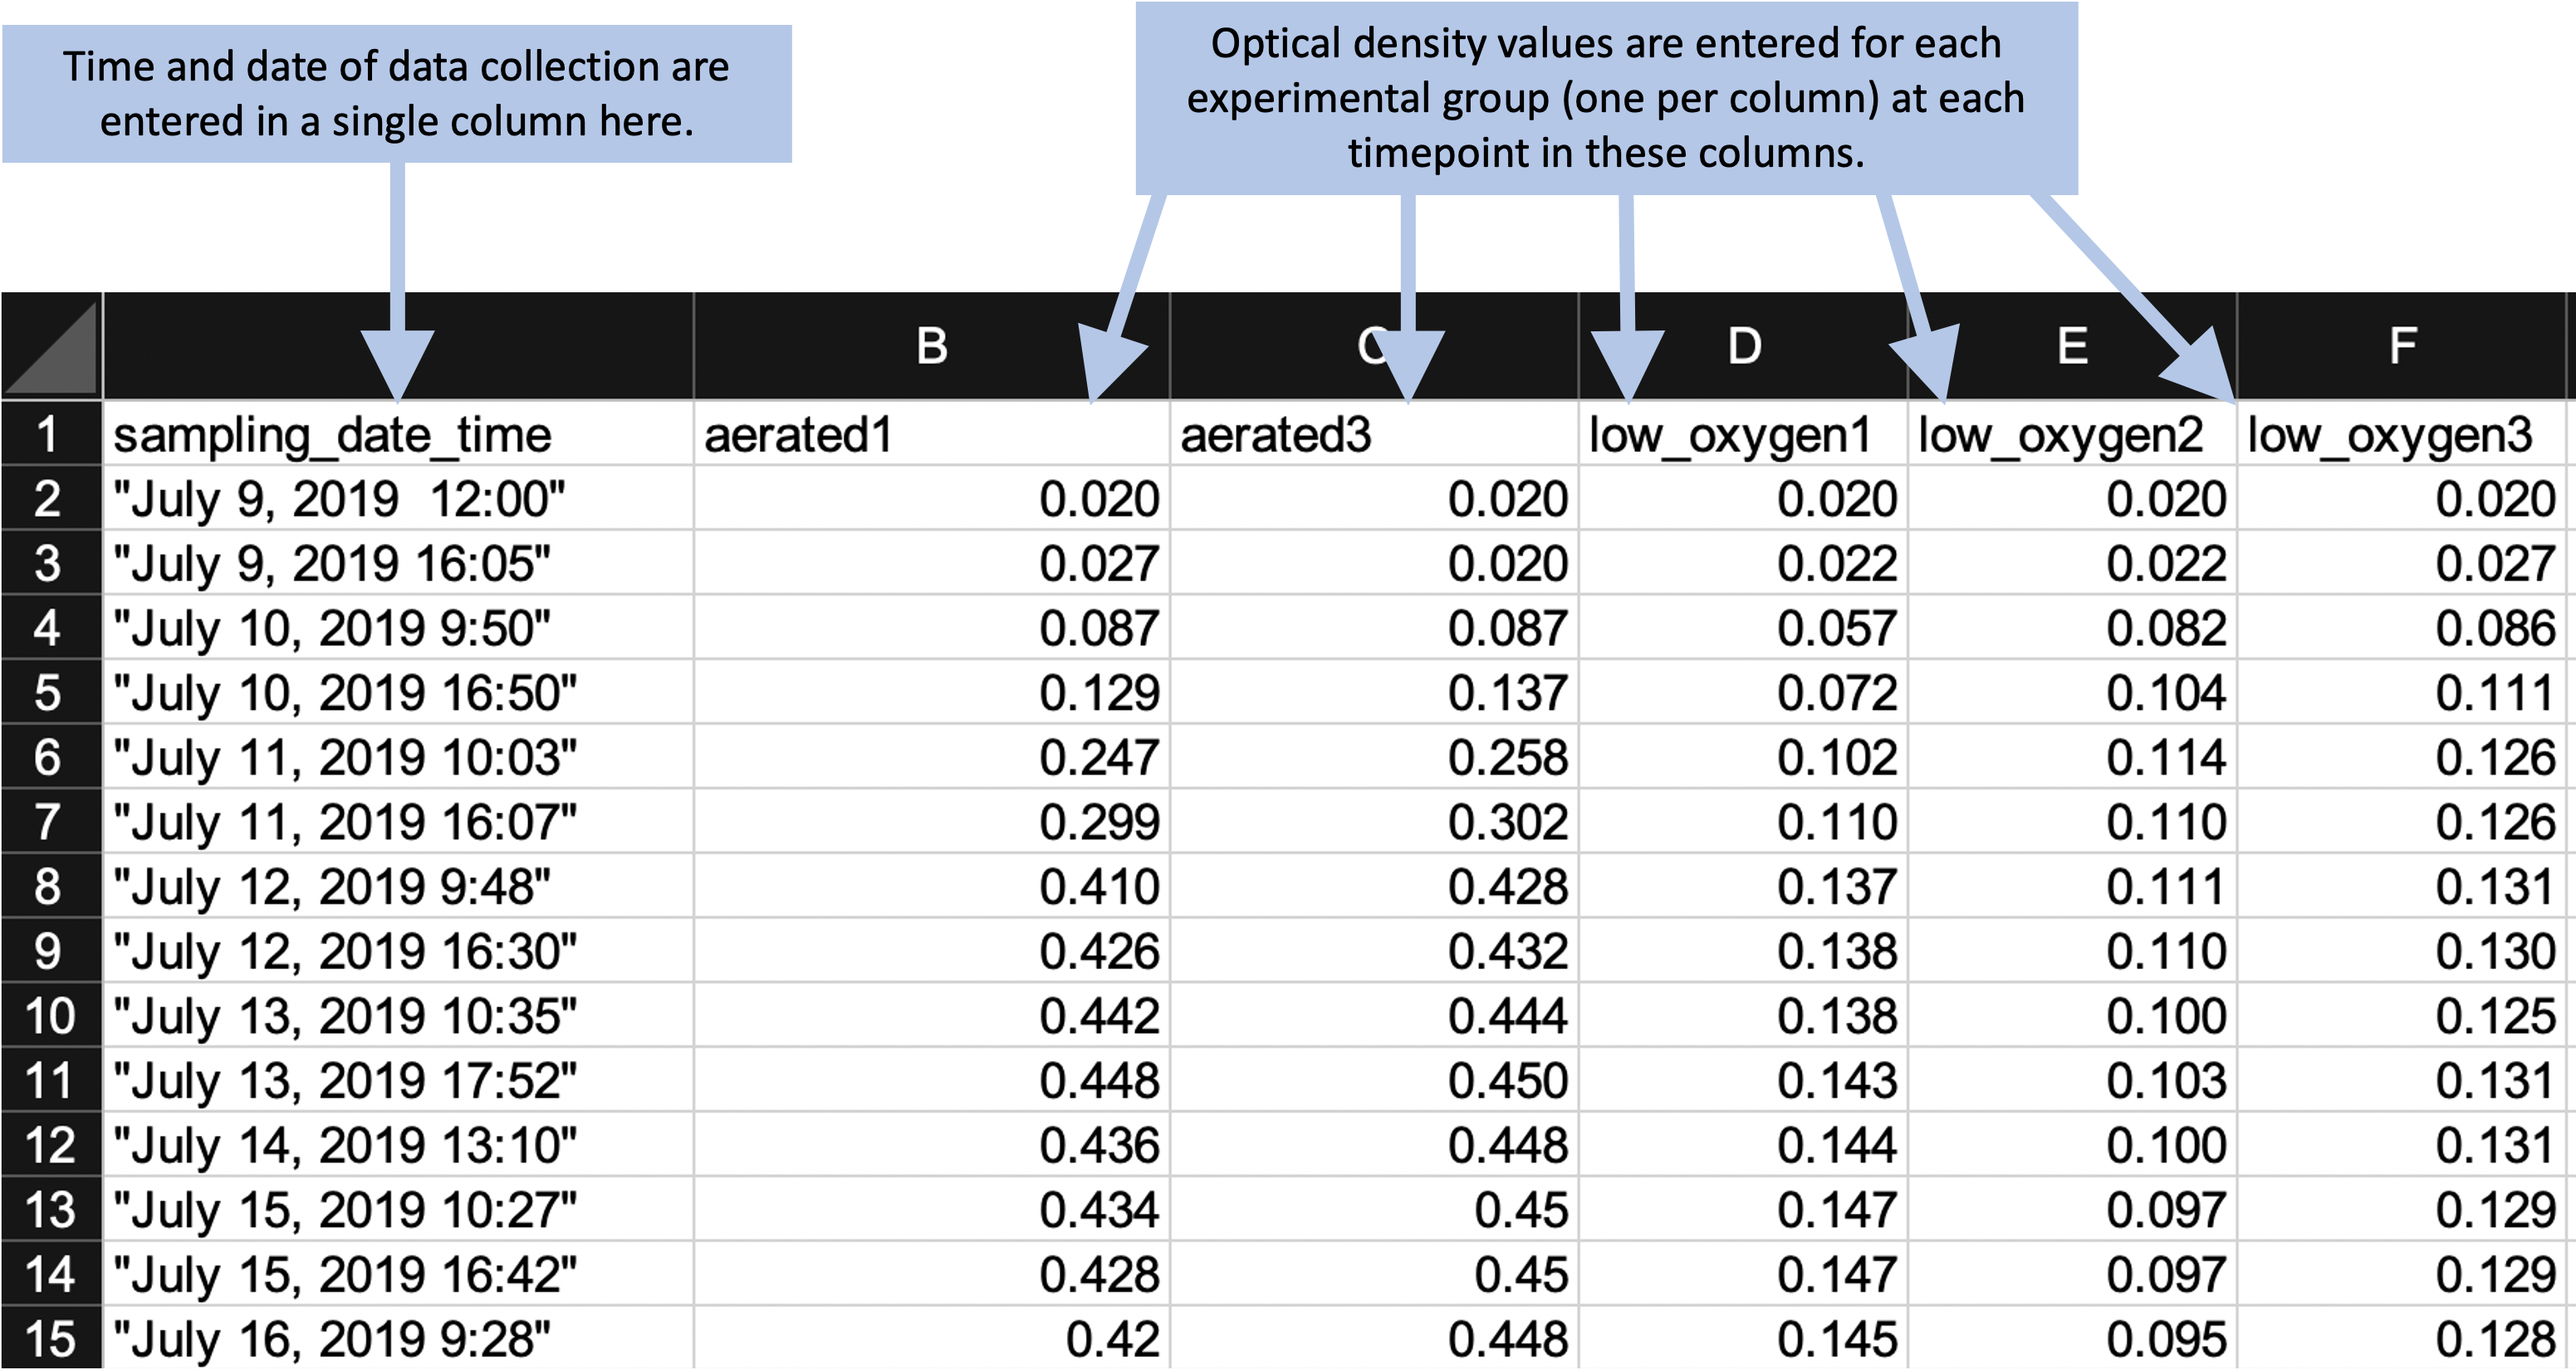
\includegraphics[width=\textwidth]{figures/growth_curve_simple} \caption[Example of an simpler format that can be used to record and analyze data for the same laboratory experiment as the previous figure]{Example of an simpler format that can be used to record and analyze data for the same laboratory experiment as the previous figure. Annotations highlight where data is entered by hand. No calculations are conducted or figures created---these are all done later, using a code script.}\label{fig:growthsimple2}
\end{figure}

\subsection{Separating data analysis from data collection}\label{separating-data-analysis-from-data-collection}

Once you have created a ``tidy'' template for collecting your data in the
laboratory, you can create a report template that will input that data and then
provide summaries and visualizations. This allows you to separate the steps (and
files) for collecting data from those for analyzing data. Figure
\ref{fig:growthreport2} shows an example of the output of a report template
that could be created to pair with the data collection template shown in Figure
\ref{fig:growthsimple2}.

\begin{figure*}
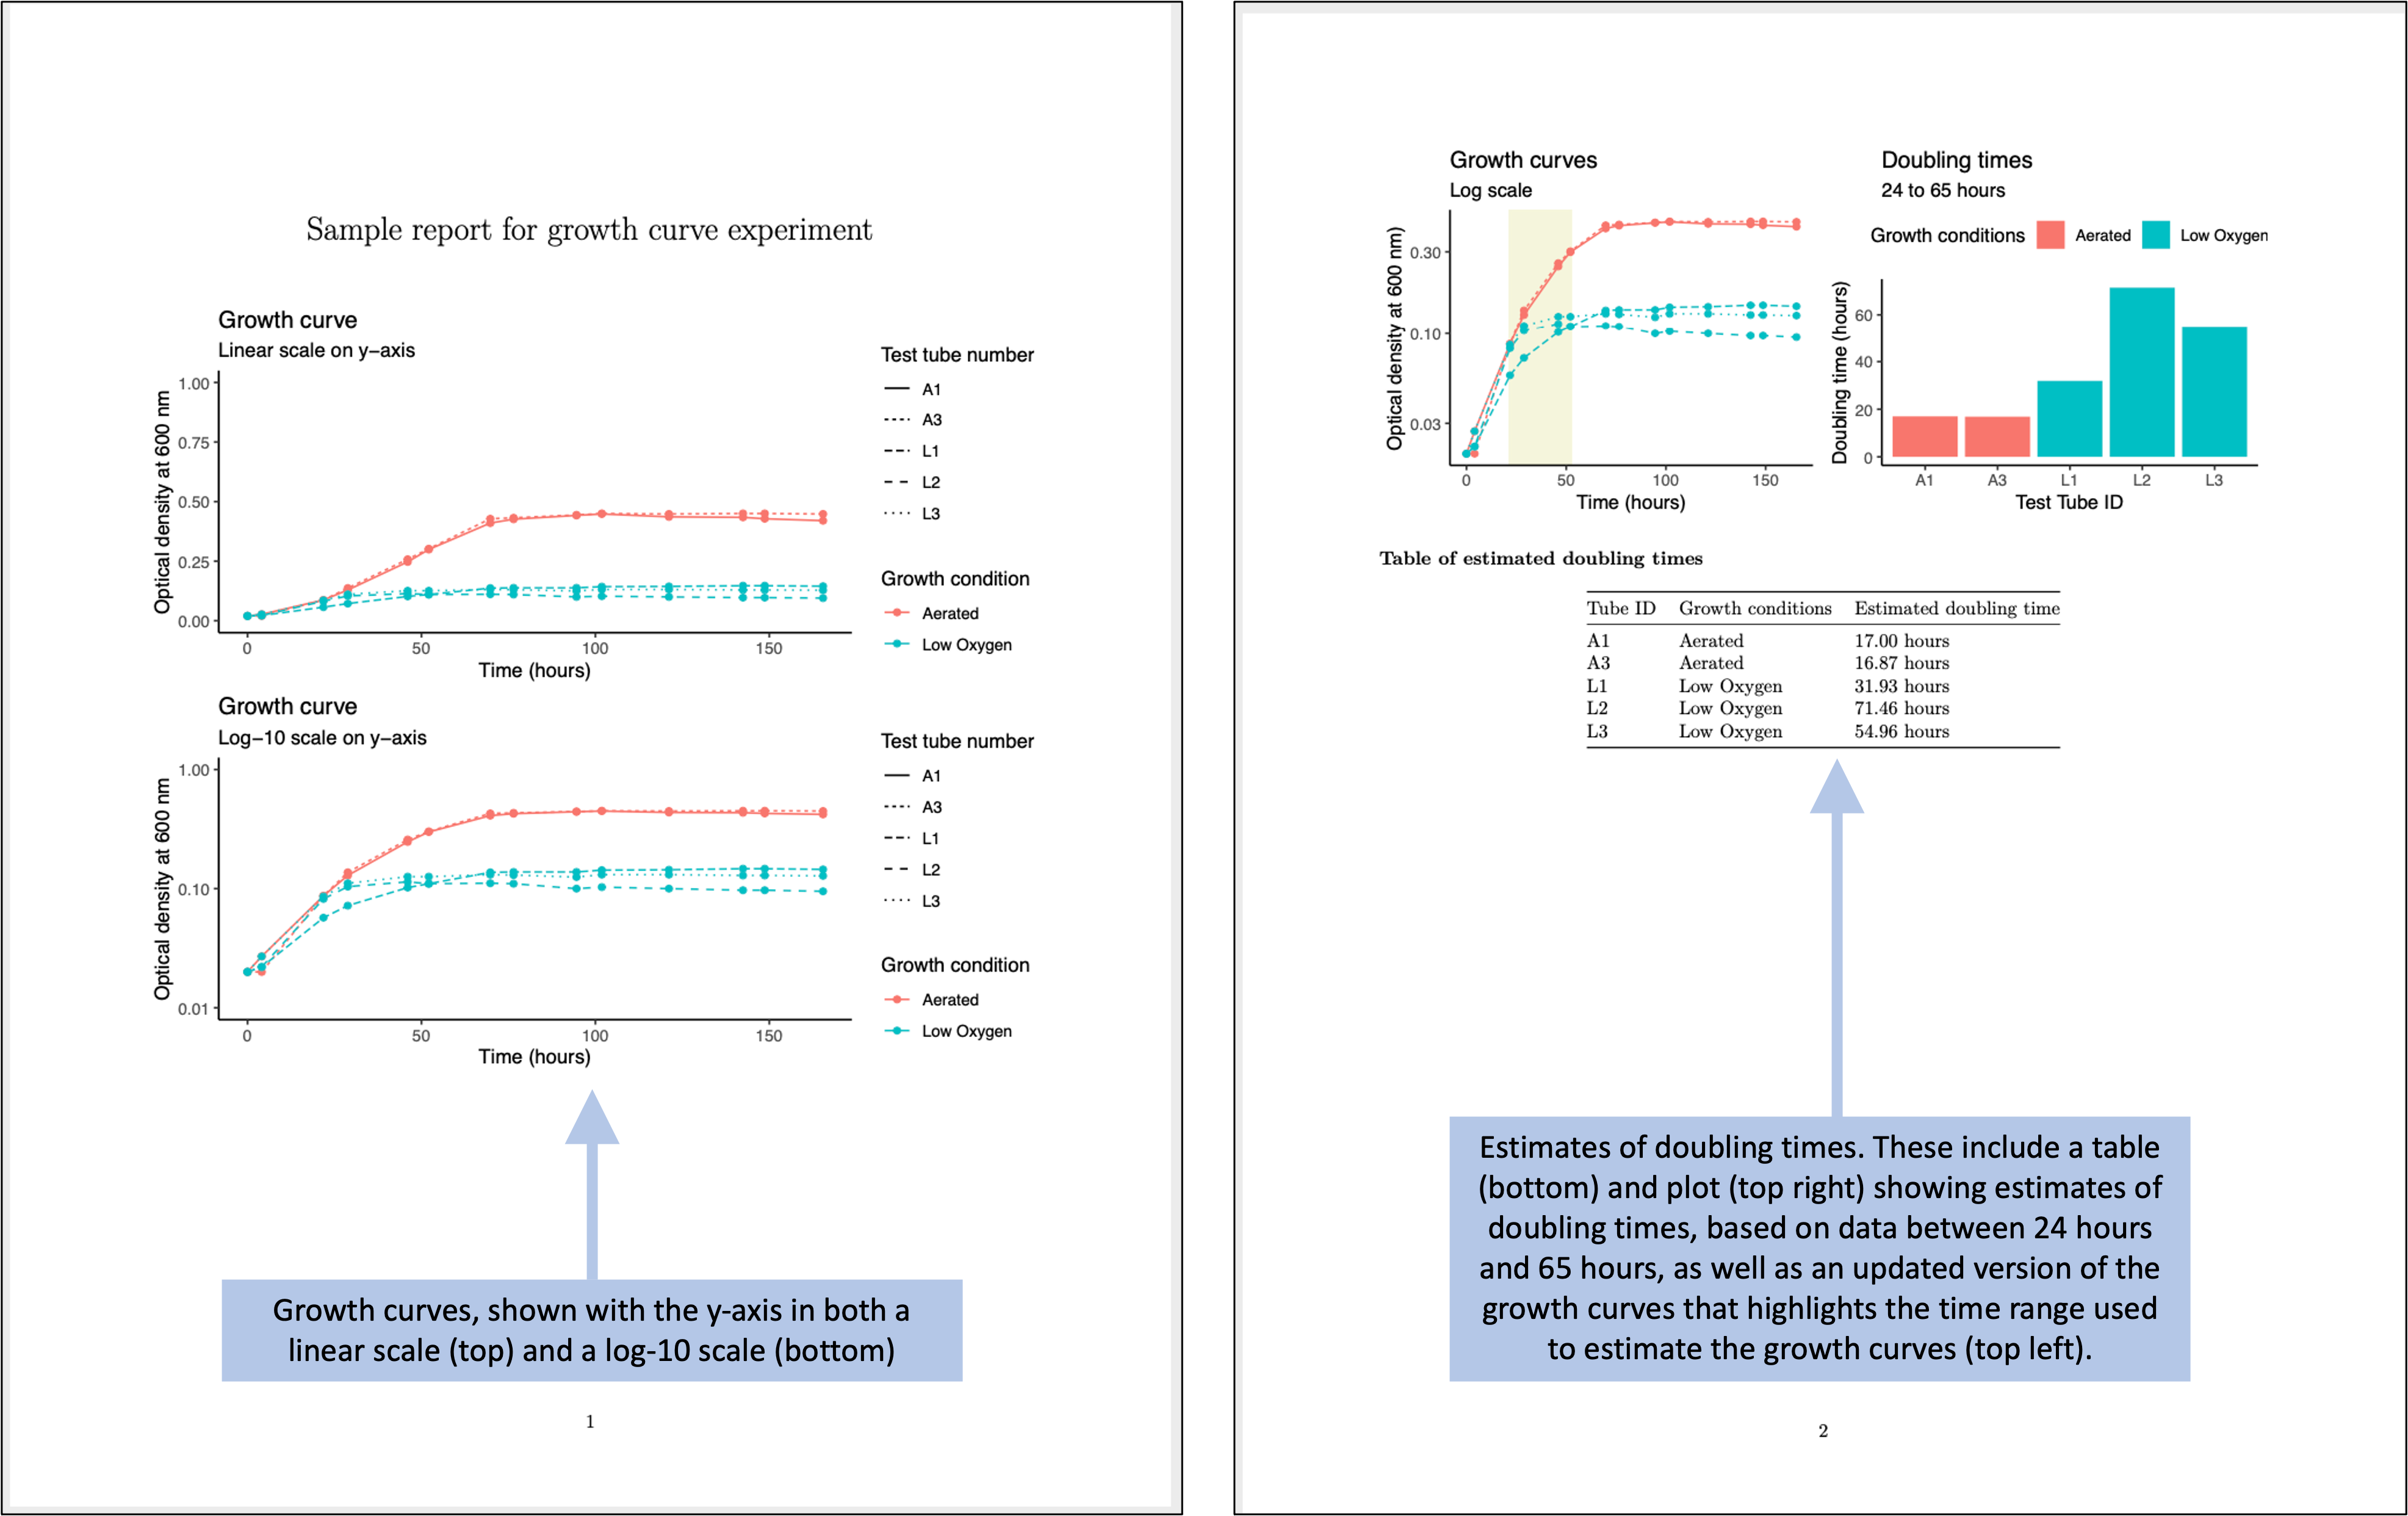
\includegraphics[width=\textwidth]{figures/growth_curve_report} \caption[Examples of an automated report that can be created to quickly generate summaries and estimates of the data collected in the simplified data collection template for the example experiment]{Examples of an automated report that can be created to quickly generate summaries and estimates of the data collected in the simplified data collection template for the example experiment.}\label{fig:growthreport2}
\end{figure*}

To create a report template like this, you can use tools for reproducible
reports from statistical programs like R and Python. In this section, we will
give an overview of how you could create the report template shown in Figure
\ref{fig:growthreport2}.

This report is written using a framework called RMarkdown, which allows you to
include executable code inside a nicely-formatted document, resulting in a
document in Word, PDF, or HTML that is easy for humans to read while also
generating results based on R code. We will cover this format in details in
modules 3.7--3.9. The code used to generate the results in Figure
\ref{fig:growthreport2} is all in the programming language R. Module 3.3
provides guidance on getting started with R, if you have not used it before.

A programming language can seem, at first glance, much more difficult to learn
and use than using a spreadsheet program like Excel to set up formulae and
macros. However, languages like R have evolved substantially in recent years to
allow for much more straightforward coding than you may have seen in the past,
and the barrier to learning to use them for straightforward data management and
analysis is not much higher than the effort required to become proficient in
using a spreadsheet program. To demonstrate this, let's look through a few of
the tasks required to generate the results shown in Figure
\ref{fig:growthreport2}. We won't cover all the code, just highlight some of
the key steps. If you'd like to look in details over the code and the output
document, you can download those files and explore them: you can access the file
for the \href{https://github.com/geanders/improve_repro/blob/master/data/growth_curve_data_in_excel\%20(1)/Example_report.Rmd}{Rmarkdown
file},
and you can download the \href{https://github.com/geanders/improve_repro/raw/master/data/growth_curve_data_in_excel\%20(1)/Example_report.pdf}{output
PDF}.
If you'd like to try out the code in the Rmarkdown file, you'll also need the
example data, which you can download by clicking
\href{https://github.com/geanders/improve_repro/raw/master/data/growth_curve_data_in_excel\%20(1)/growth\%20curve\%20data_GR.xls}{here}.

One key step is to read the collected data into R. When you use a spreadsheet
for both data collection and analysis, you don't need to read the data to start
working with them, since everything is saved in the same file. Once you separate
the steps of data collection and data analysis, however, you do need to take an
extra step to read the data file into another program for analysis. Fortunately,
this is very simple in R. The data in this example are recorded using an Excel
spreadsheet, and there is a simple function in R that lets you read data in from
this type of spreadsheet (Figure \ref{fig:growthreadexcel}). After this step of
code, you will have an object in R called \texttt{growth\_data}, which contains the data
in a two-dimensional form very similar to how it is recorded in the spreadsheet
(this type of object in R is called a dataframe).

\begin{figure*}
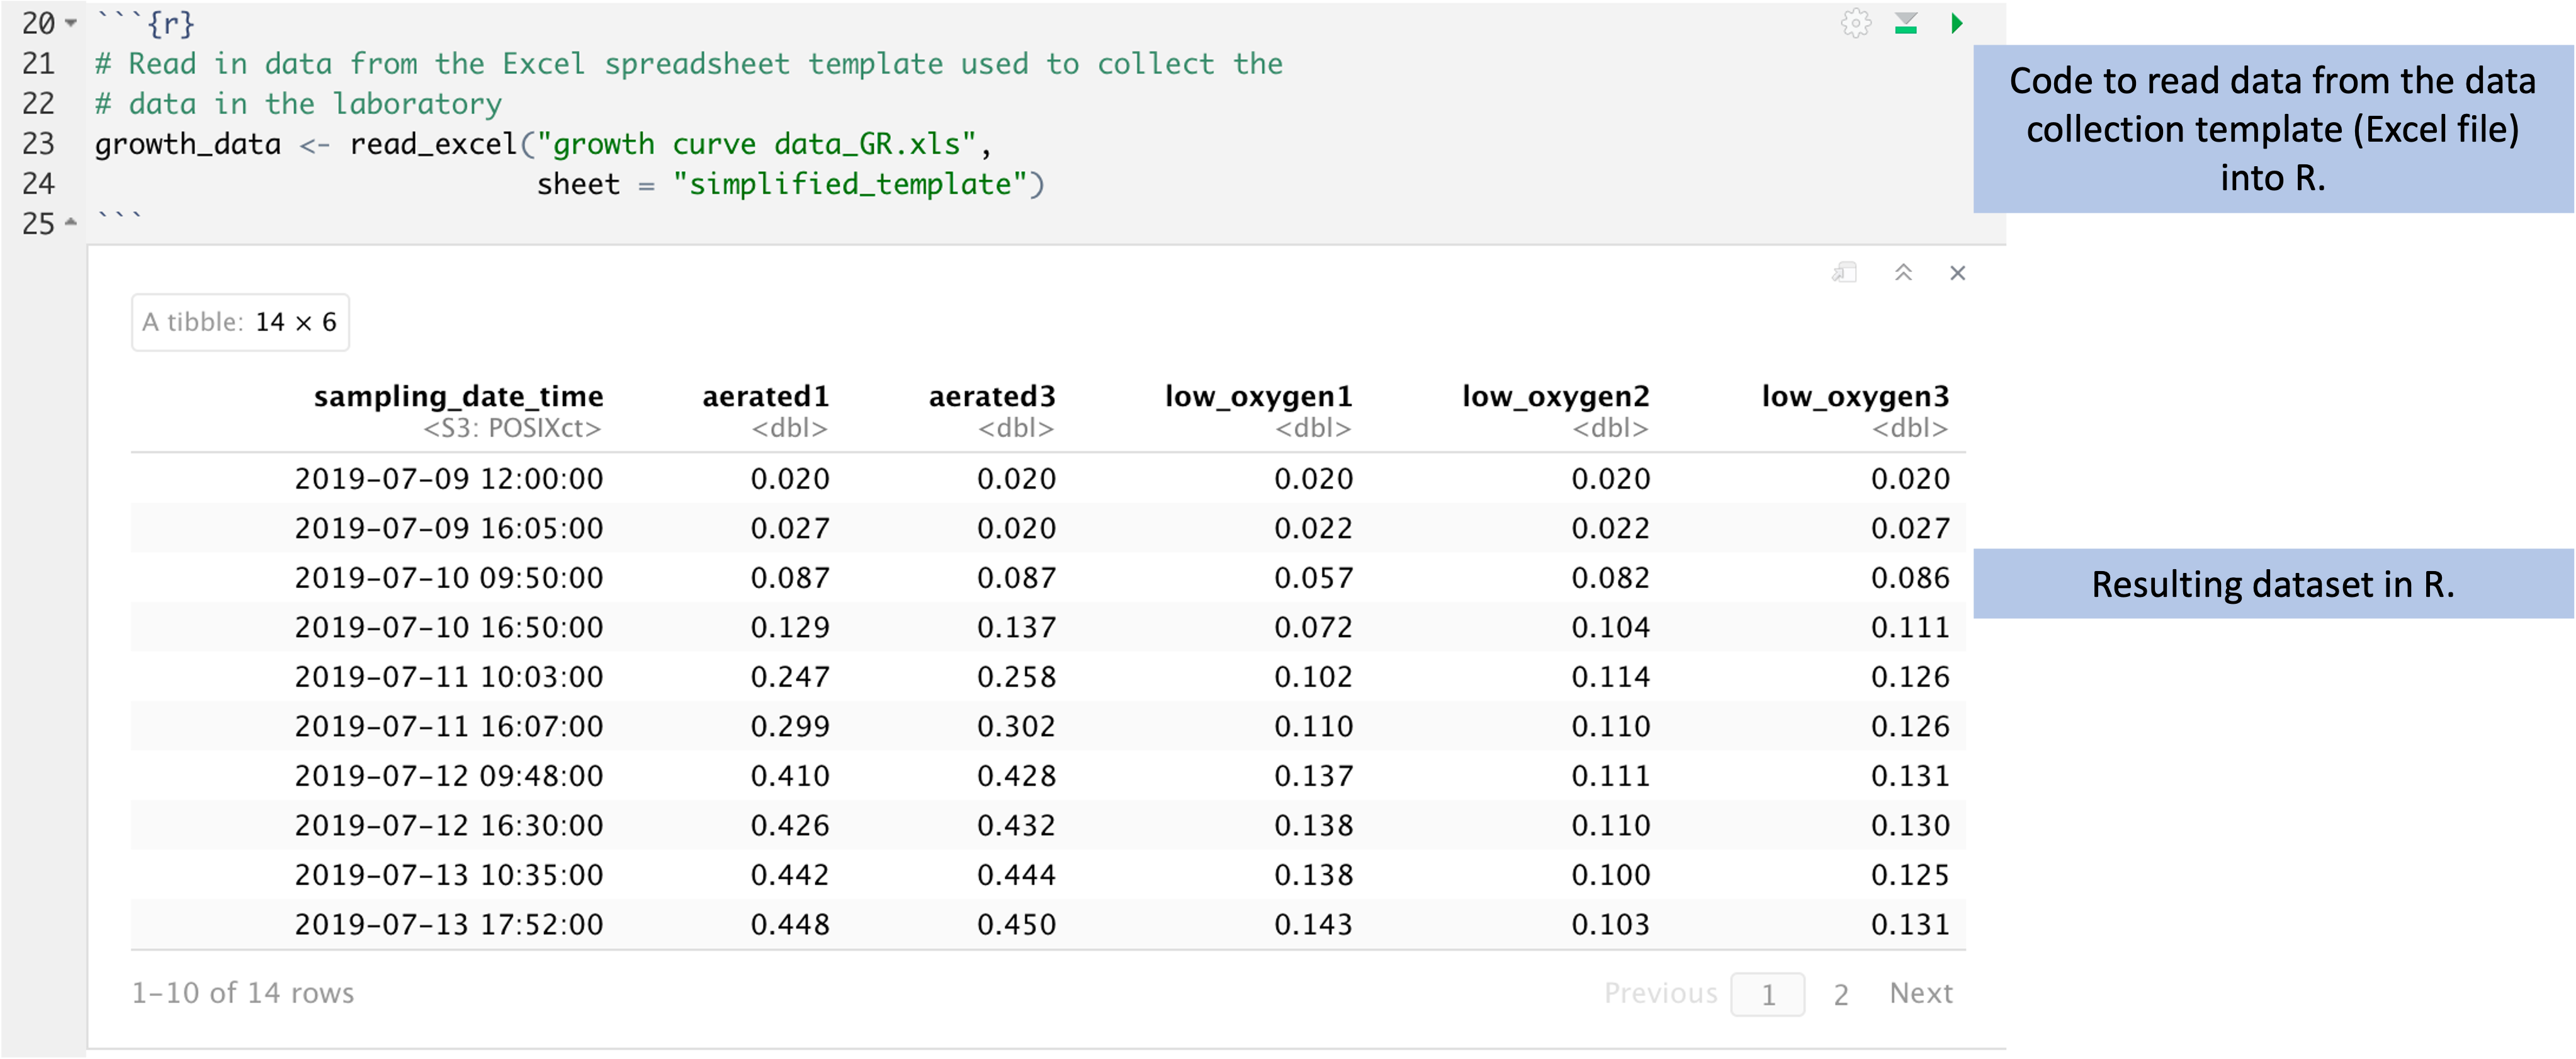
\includegraphics[width=\textwidth]{figures/growth_curve_readxl} \caption[Code to read data from the data collection template into R for cleaning, analysis, and visualization]{Code to read data from the data collection template into R for cleaning, analysis, and visualization. The data were recorded in the tidy data collection template described earlier in this module. Here, those data are read into R (code shown at top). The resulting data in R are stored in a format that is very similar to the design of a spreadsheet, with rows for observations and columns for the values recorded for each observation (bottom).}\label{fig:growthreadexcel}
\end{figure*}

Another key step is to calculate, for each observation, the time since the start
of the experiment. In the original data collection template shown in Figure
\ref{fig:growthexcel2}, this calculation was done by hand by the researcher and
entered into the spreadsheet. When we converted the spreadsheet to a tidier
version, we took out all steps that involved calculations with the data, and
instead limited the data collection to only raw, observed values. This helps us
avoid errors and typos---instead of having the researcher calculate the
difference in time as they are running the experiment, they can just record the
time, and we can write code in the analysis document that handles the further
calculations, using well-designed and well-tested tools to do this calculation.

Figure \ref{fig:growthadddifftime} shows code that can be used for this
calculation. At the start of this code, the data are stored in an object named
\texttt{growth\_data}. The \texttt{mutate} function adds a column to the data, named
\texttt{sampling\_delta\_time}, that will give the difference between the time of an
observation and the start of the experiment. Within the \texttt{mutate} call, a special
function named \texttt{difftime} calculates the difference in two time points. This
function lets us specify the time units we'd like to use, and here we can pick
\texttt{"hours"} for the units. The \texttt{first} function lets us pull out the first value
in the data for a recorded time---in other words, the time when the experiment
started. This lets us compare each observation time to the time of the start of
the experiment. The result of this code is a new version of the \texttt{growth\_data}
dataframe, with a new column giving time since the start of the experiment:

\begin{figure*}
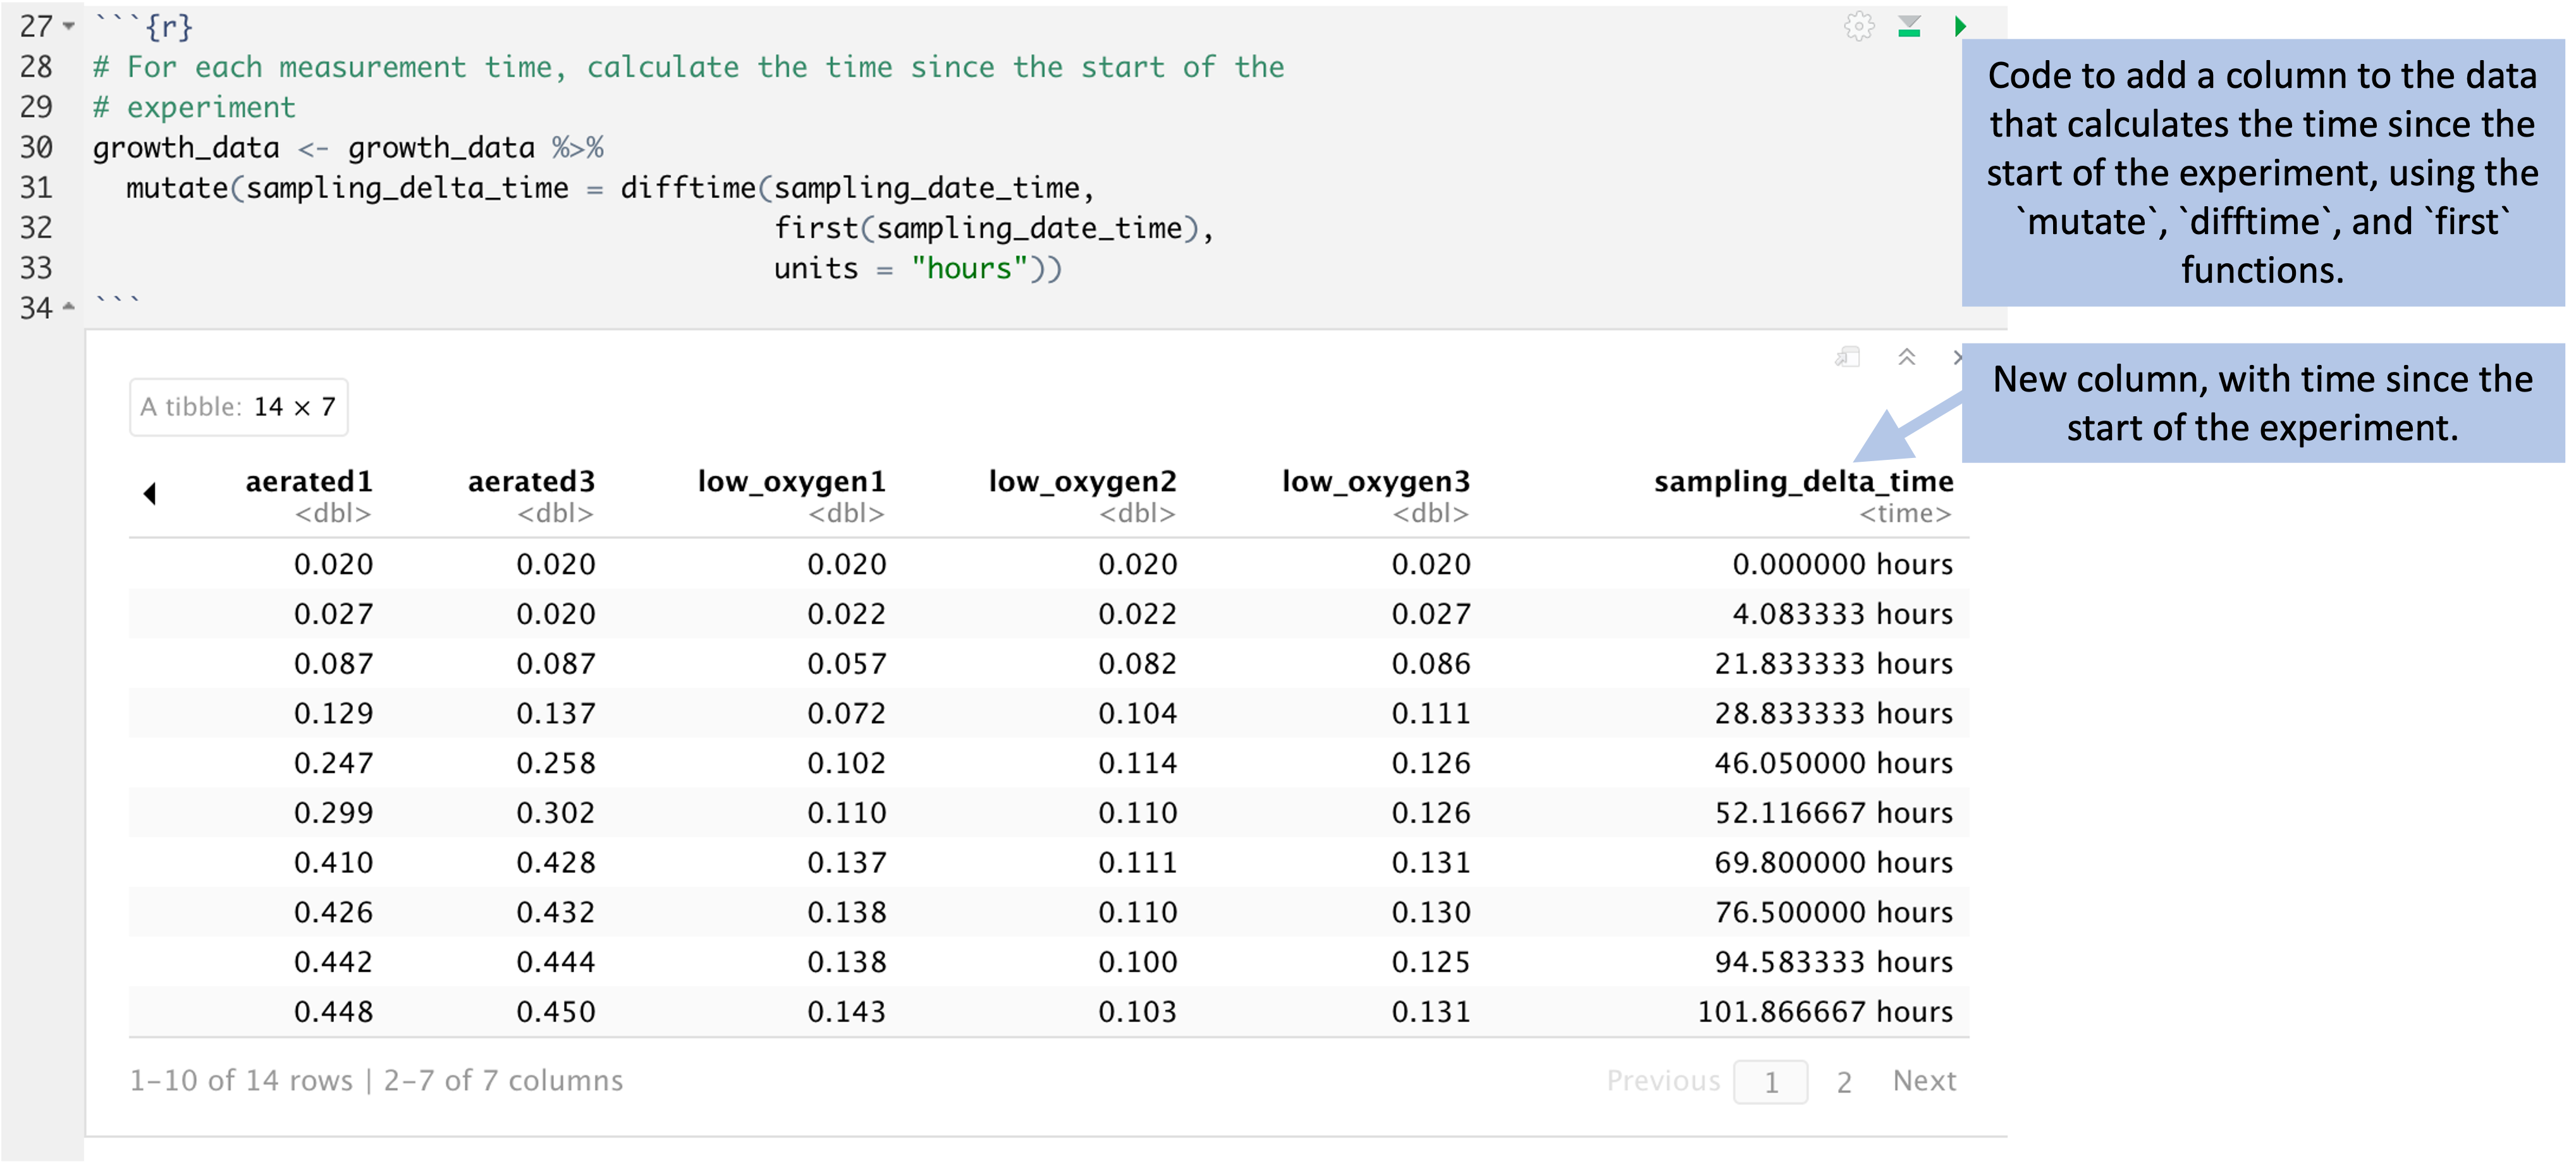
\includegraphics[width=\textwidth]{figures/growth_curve_adddifftime} \caption[Code to add a column to the data that gives the time since the start of the experiment]{Code to add a column to the data that gives the time since the start of the experiment. This code (top) uses the time recorded for each experiment and compares it to the first recorded time, at the start of the experiment. This determines the time since the start of the experiment for each observation, given in a new column in the data (bottom).}\label{fig:growthadddifftime}
\end{figure*}

Another key step is to plot results from the data. In R, there is a package
called \texttt{ggplot2} that provides tools for visualization. The tools in this
package work by building a plot using ``layers'', adding on small elements
line by line through simple functions that each do one simple thing.
While the resulting code can be long, each step is simple, and so it
becomes simple to learn these different ``layers'' and learn how to combine
them to create complex plots.

Figure \ref{fig:growthplotcode} walks through the code for one of the
visualizations in the report. At this point in the report code, the data have
been reformatted into an object called \texttt{growth\_data\_tidy}, which has columns for
each observation on the time since the start of the experiment
(\texttt{sampling\_delta\_time}), the measured optical density (\texttt{optical\_density}),
whether the tube was aerated or low oxygen (\texttt{growth\_conditions}), and a short ID
for the test tube (\texttt{short\_tube\_id}). The code starts by creating a plot object,
specifying that in this plot the color will show the growth conditions, the
position on the x-axis will show the time since the start of the experiment, and
the y-axis will show the optical density. Layers are then added to this plot
object that add points and lines to the plot based on these mappings, and for
the lines, it's further specified that the type of line should show the test
tube ID (for example, one tube will be shown with a dotted line, another with a
dashed line). Further layers are added to customize the scale labels with
\texttt{labs}, including the labels for the x-axis and y-axis and the legends of the
color and linetype scales. Another layer is used to customize the appearance of
the plot---things like the background color and the font used---and another
layer is added to use a log-10 scale for the x-axis.

\begin{figure*}
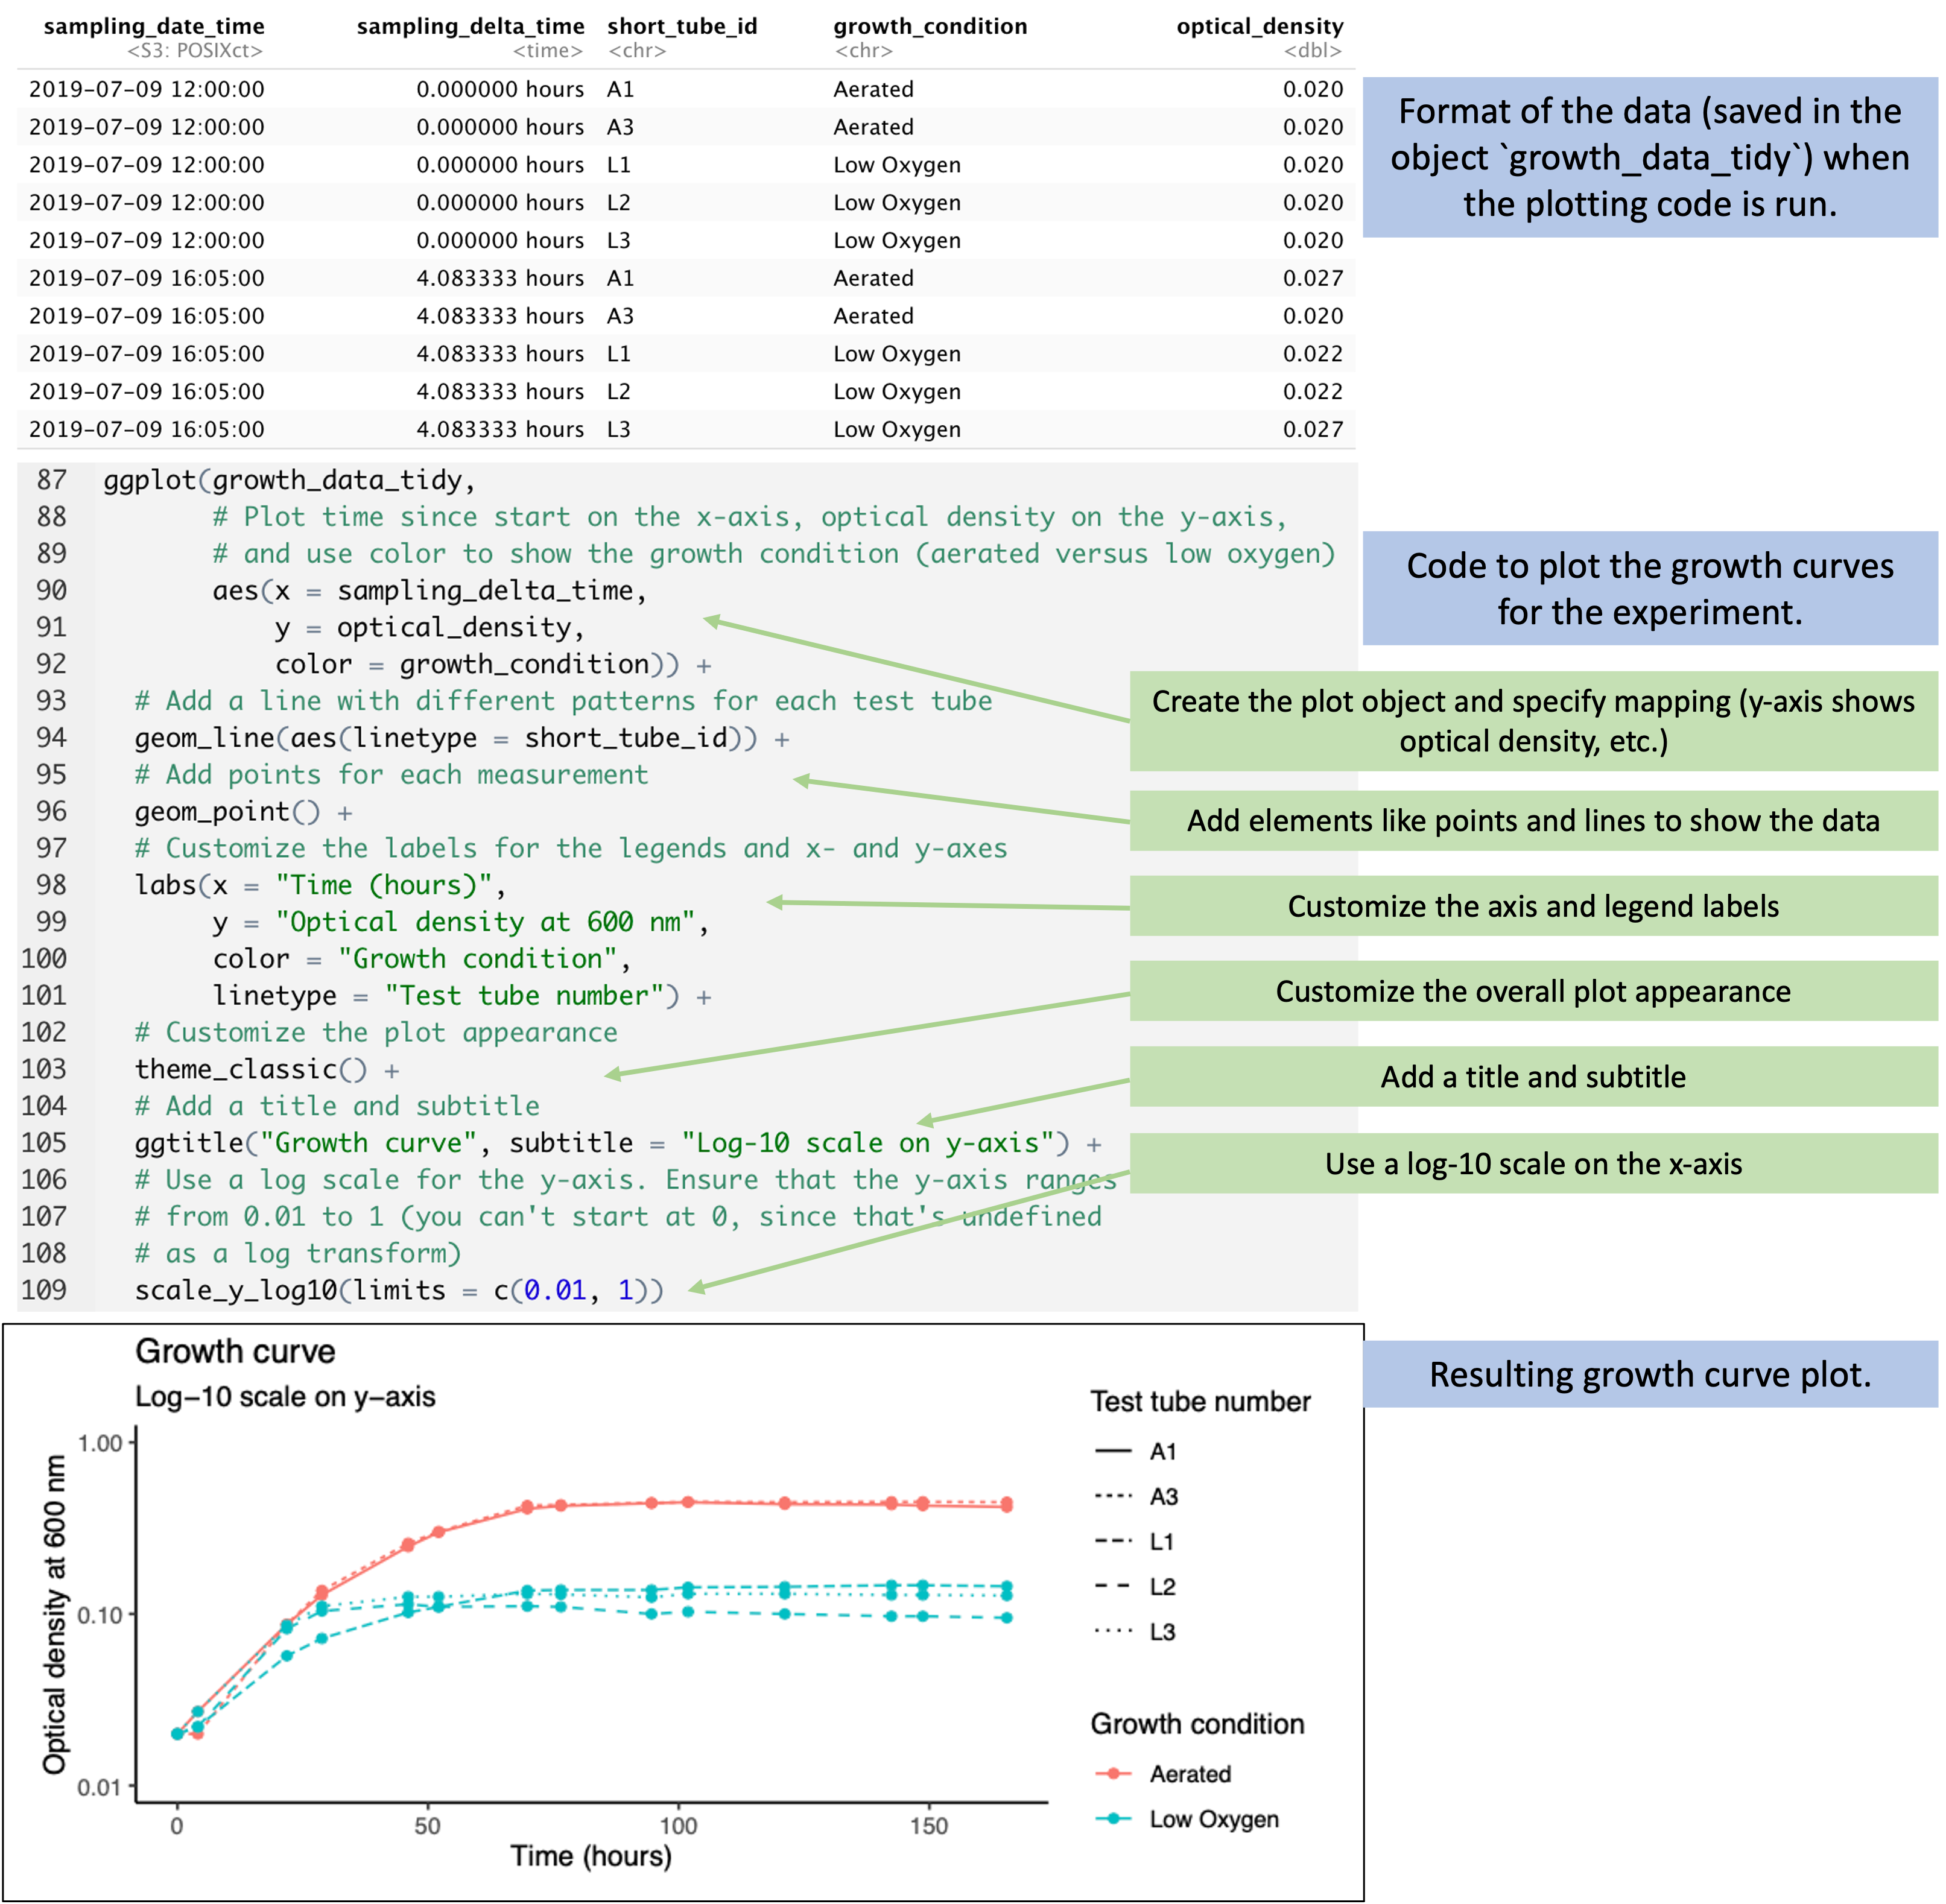
\includegraphics[width=\textwidth]{figures/growth_curve_plot_code} \caption[Code to plot growth curves from the data]{Code to plot growth curves from the data. When the plotting code is run, the data have been transformed into a 'tidy' format (top), with columns that include the time since the start of the experiment, a test tube ID, the growth condition for the test tube, and the optical density measured in that test tube. The code (middle) add layers to implement each element of the plot based on this input data. The final plot is shown at the bottom.}\label{fig:growthplotcode}
\end{figure*}

While this looks like a lot of code, the process isn't any longer than it would
be to customize elements of a plot in a spreadsheet program. The advantages of
the coded approach are that you maintain a full record of all the steps you took
to customize the plot. This is something that you can use to reproduce your plot
later, or even to use as a starting point for creating a similar plot with new
data.

The next key step that we'd like to point out is how you can write and use small
functions to do customized tasks for the experimental data. As one example, for
the data in this example, we want to estimate doubling times based on the
observed data. The principal investigator has decided that we should do this
based on comparing bacteria levels at two times points---the measured time that
is closest to 65 hours after the start of the experiment, and the time that is
closest to 24 hours after the start of the experiment.

In the original data collection template---where the data were both recorded
and analyzed in a spreadsheet---this step was done by hand by the researcher,
looking through the data and selecting the cell closest to each of these
times, and then connecting that cell to a spreadsheet formula calculation
to calculate the doubling time. We can make this process more rigorous and
less prone to error by writing a small function that does the same thing,
then using that function to automate the process of identifying the
relevant observations to use in calculating the doubling rate.

Figure \ref{fig:growthfunction} shows how you can write and then use a small
function in R. This function will input your \texttt{growth\_data} dataset, as well as a
time that you are aiming for, and will output the sampling time in the data that
is closest to---while not larger than---that time. It does that in a few steps
within the body of the function. First, the code in the function filters to only
observations earlier than the target time. Then it measures the difference
between each of the times for these observations and the target time, and uses
this to identify the observation with the closest time to the target. It pulls
out the time of this observation and returns it.

\begin{figure*}
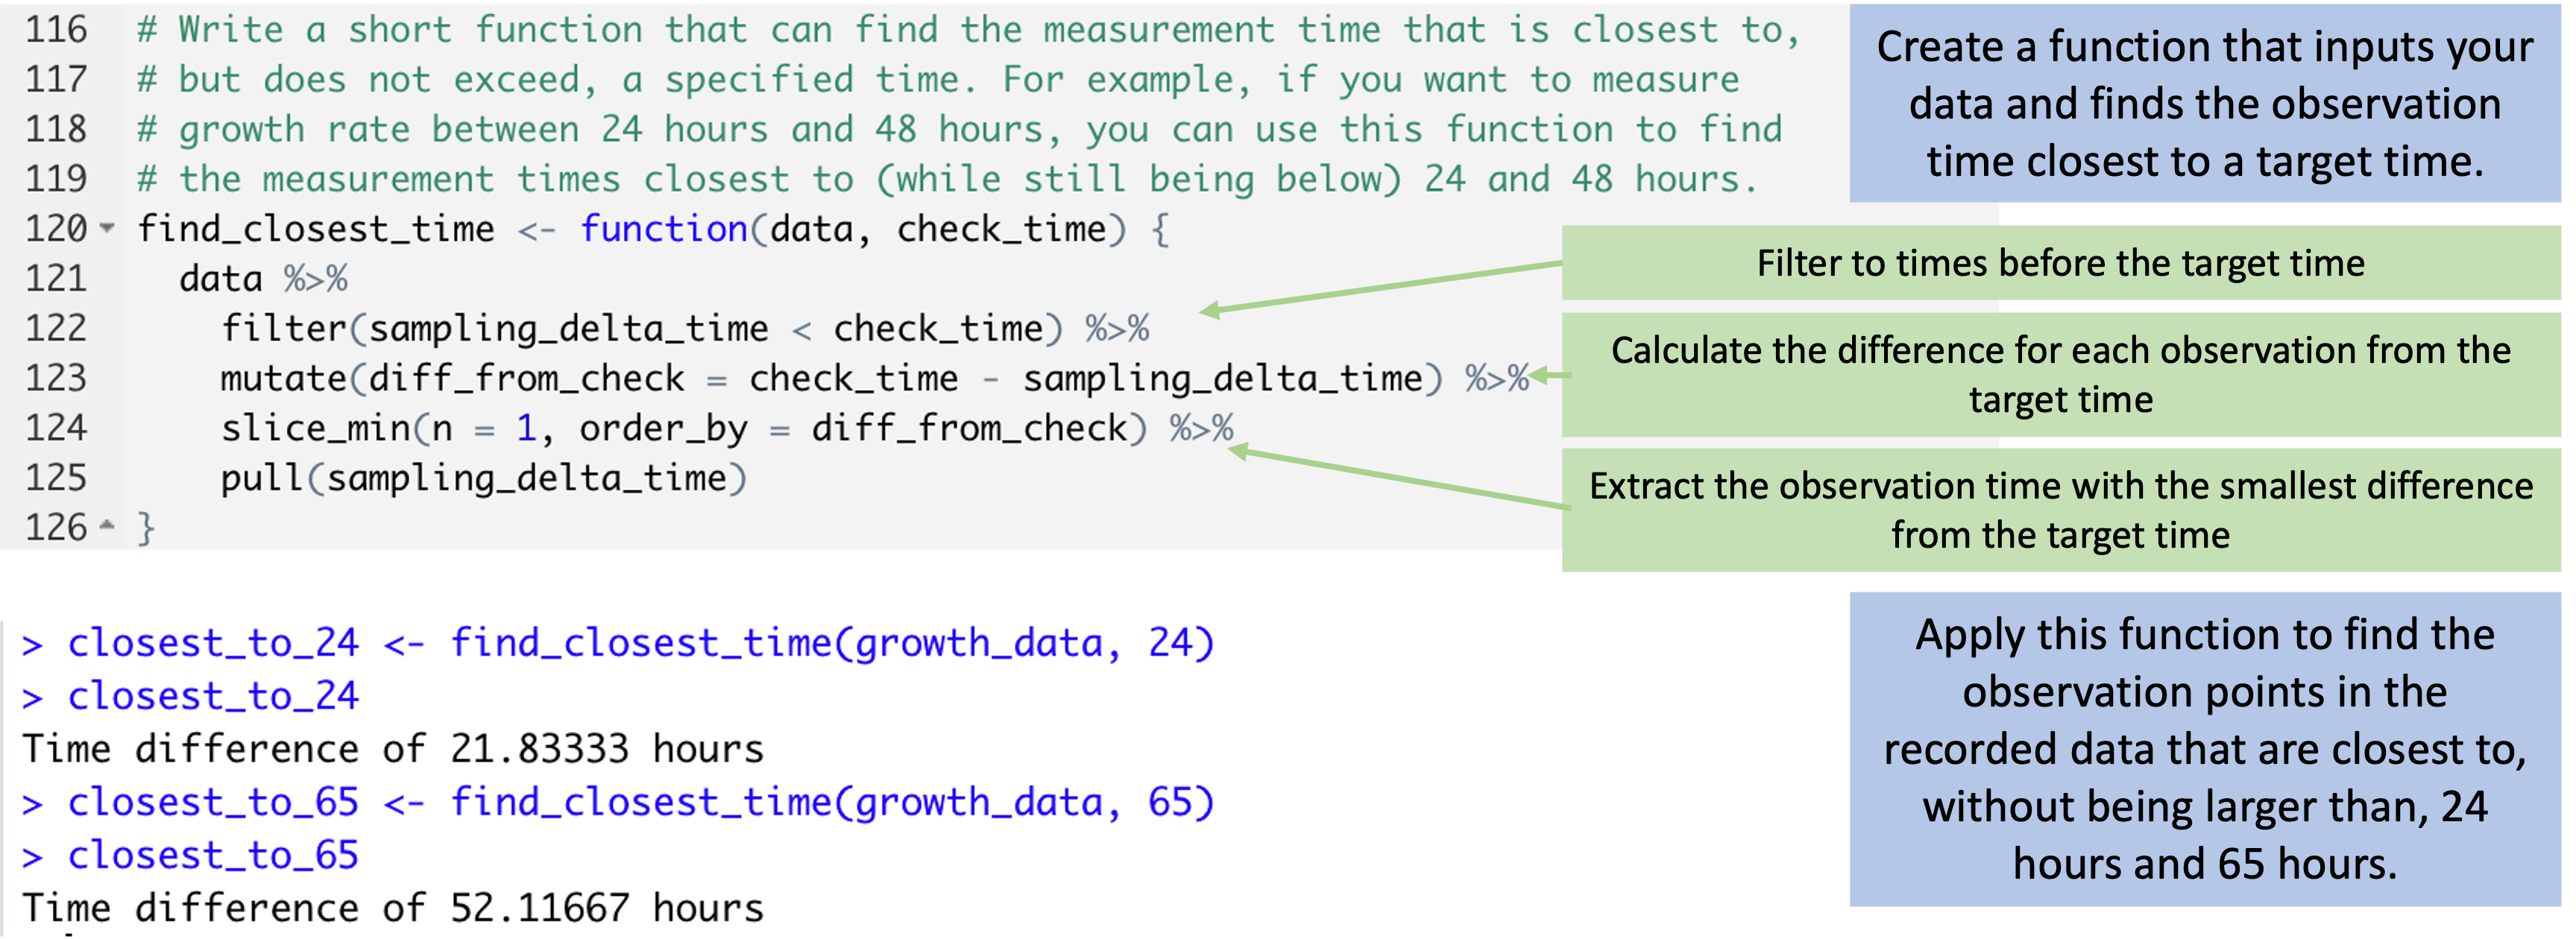
\includegraphics[width=\textwidth]{figures/growth_curve_function} \caption[Code to create and apply a small function]{Code to create and apply a small function. The code at the top can be used to create a function that can input your dataframe and determine the observation time in that data that is closest to (without being larger than) a target time. The function does this through a series of small steps. This function can then be applied to find the observation time in the data that is closest to specific target times, like 24 hours and 64 hours (bottom).}\label{fig:growthfunction}
\end{figure*}

Small functions like this can easily be reused in other code for your research
group. By writing the logic of the step out as a function---rather than redoing
the steps by hand or step-by-step each time you need to do it---you can save
time later, and in return, you have extra time that you can spend in writing
the original function and carefully checking to make sure that it works
correctly.

Finally, many of these steps require extensions to base R. When you download R,
you are getting a base set of tools. Many people have developed helpful
extensions that build on this base. These are stored and shared in what are
called \emph{R packages}. You can install these extra packages for free, and you
use the \texttt{library} function in R to load a package you've installed, giving you
access to the extra functions that it provides. Figure
\ref{fig:growthloadpackage} shows the spot in the Rmarkdown code where we
loaded packages we needed for this report. These include packages with functions
to read data in R from Excel (the \texttt{readxl}) package, as well as a suite of
packages with tools for cleaning and visualizing data (the \texttt{tidyverse} package).
In later modules, we'll talk some more about R coding tools that you might find
useful for working with biomedical data, including the tools in the powerful and
popular \texttt{tidyverse} suite of packages.

\begin{figure*}
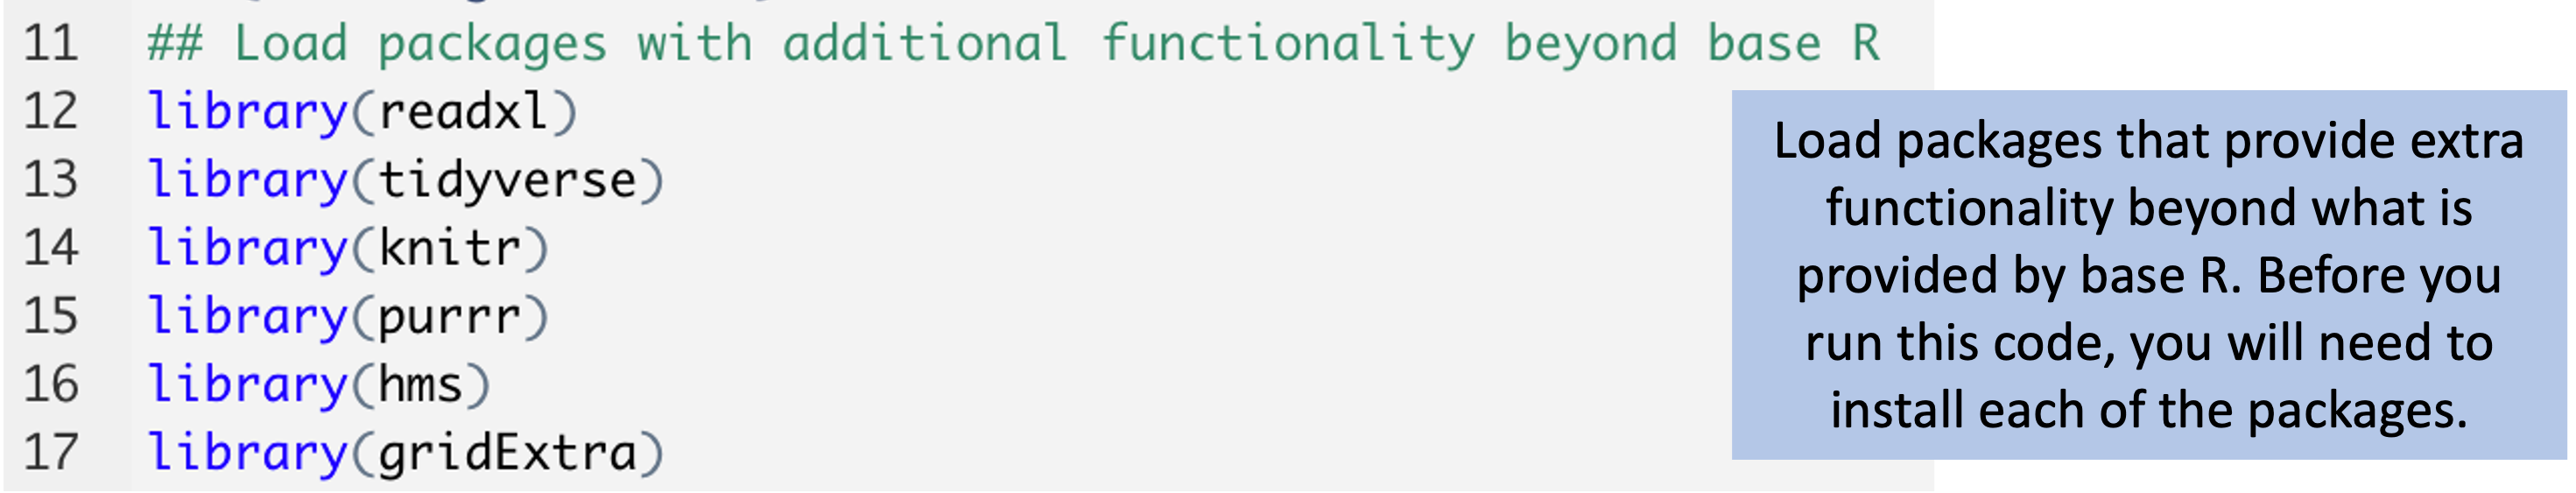
\includegraphics[width=\textwidth]{figures/growth_curve_load_packages} \caption[Code to load packages with additional functionality]{Code to load packages with additional functionality. These provide functions that are not offered in base R, but that are useful in working with the example data. They include packages with functions for reading in data from an Excel file, as well as packages with functions for cleaning and visualizing data.}\label{fig:growthloadpackage}
\end{figure*}

Overall, you can see that the code in this document provides a step-by-step
recipe that documents all the calculations and cleaning that we do with the
data, as well as how we create the plots. This code runs every time we create
the report shown in Figure \ref{fig:growthreport2}, and it gives us a good
starting point if we run additional experiments that generate similar data.

\subsection{Applied exercise}\label{applied-exercise}

The Rmarkdown document includes a number of other steps, and you might find
it interesting to download the document and the example data and walk through
them to get a feel for the process. All the steps are documented in the
Rmarkdown document with extensive code comments, to explain what's happening
along the way.

\section{Organizing project files}\label{module6}

In earlier modules, we discussed how to separate data collection from data
analysis. By separating data collection and analysis into separate files, we can
make the file for each step simpler. Further, by separating steps into different
files, we can save the files in plain text, which makes it easier to track them
using version control software (discussed in later modules). This helps create a
record of changes made to the data or analysis code during the research process.

While this process helps in reproducibility, it results in more files being
collected for an experiment. Instead of data and its analysis collected within a
single spreadsheet file, you may end up with multiple files of data collected
from the experiment, as well as separate files with scripts for processing,
analyzing, and visualizing the data. With more complex experiments, there may be
different data files containing the data collected from different assays. For example,
you may run an experiment where you collect data from each research animal on
bacterial load, as well as flow cytometry data, as well as a measure of antibody
levels through ELISA. As a result, you may have one raw data file from each
assay and, for some assays, even one file per study subject (e.g., flow
cytometry). The files for a research project will also include files with
writing and presentations (posters and slides) associated with the project, as
well as code scripts for pre-processing data, for conducting data analysis, and
for creating and sharing final figures and tables.

In this and the next few modules, we'll discuss how you can organize the files
for an experiment using a single directory that is designed to follow a similar
format across all your projects. The modules will discuss the advantages of
well-designed project directories, tips for arranging files within a project
directory, and how to create a directory template that allows you to use
consistent file organization across many experiments.

\textbf{Objectives.} After this module, the trainee will be able to:

\begin{itemize}
\tightlist
\item
  Explain how poor file organization can impede reproducibility
\item
  List benefits of good file organization
\item
  List several principles for organizing research project files
\item
  Define the design concept of ``discoverability''
\item
  Apply the idea of discoverability in organizing project files
\item
  Explain how a project directory template works
\end{itemize}

\subsection{Advantages of organizing project files}\label{advantages-of-organizing-project-files}

As the files for a project accumulate, do you have a clear plan for keeping them
organized? Based on one analysis, many biomedical researchers do not. One study,
for example, surveyed over 250 biomedical researchers at the University of
Washington. They noted that, ``Some researchers admitted to having no
organizational methodology at all, while others used whatever method best suited
their individual needs'' \citep{anderson2007issues}. One respondent answered, ``They're
not organized in any way---they're just thrown into files under different
projects,'' while another said ``I grab them when I need them, they're not
organized in any decent way,'' and another, ``It's not even organized---a file on
a central computer of protocols that we use, common lab protocols but those are
just individual Word files within a folder so it's not searchable \emph{per se}''
\citep{anderson2007issues}.

This lack of organization can make scientists reluctant to share their research
files, impeding reproducibility. In an article on organizing project files for
research, Marwick notes:

\begin{quote}
``Virtually all researchers use computers as a central tool in their
workflow. However, our formal education rarely includes any training in
how to organise our computer files to make it easy to reproduce results
and share our analysis pipeline with others. Without clear instructions,
many researchers struggle to avoid chaos in their file structures, and so
are understandable reluctant to expose their workflow for others to see.
This may be one of the reasons that so many requests for details about
method, including requests for data and code, are turned down or go
unanswered.'' \citep{marwick2018packaging}
\end{quote}

Sharing data and code is crucial to research reproducibility, especially for
projects that include extensive proprocessing and complex analysis of data, as
many biomedical research projects now do. As a further bonus, when research articles
include data, they tend to be more impactful, as measured by
citations that the paper receives \citep{marwick2018packaging}.

In an earlier module, we introduced Adam Savage's idea of ``knolling'' to keep a
workspace tidy (Module 2.3). He was talking about a physical workspace. When
you are working with data, computer files and directories are your workspace.
For any type of work, the design of the workspace plays a critical role in
how the workers approach tasks and solve problems. Rod Judkins, who is a
lecturer at St Martin's College of Art, highlights this in a book on
creative thinking:

\begin{quote}
``Your working environment, whether it's a supermarket, office, studio, or
building site, persuades you to work and think in certain ways. The more aware
you are of that, and the more you understand your medium, the more you can use
it to your advantage.'' \citep{judkins2016art}
\end{quote}

Adam Savage describes how important this is in another type of work: gourmet
cooking. He describes how this idea of an organized workspace is captured by the
technique of \emph{mise en place}---of laying out all the elements needed for the
work ahead of time and in an organized way---introduced by the famous French
chef August Escoffier:

\begin{quote}
``Kitchens are pressure cookers in which wasted movement and hasty technique
can ruin a dish, slice an artery, burn a hand, land you in the weeds, and
ultimately kill a restaurant. \emph{Mise en place} is the only way to reliably create
a perfect dish, to exact specifications, over and over again, night after night,
for paying customers who demand nothing less.'' \citep{savage2020every}
\end{quote}

Good organization of your files can similarly encourage clear thinking, and it
can help you in reasoning through how to analyze data. One article notes that
``mundane issues such as organizing files and directories and documenting
progress \ldots{} are important because poor organizational choices can lead to
significantly slower research progress.'' \citep{noble2009quick} In fact, if files are
organized in a consistent way across multiple projects, this can even allow you
to start automating some necessary tasks through code that is built to work with
that consistent structure \citep{buffalo2015bioinformatics}.

Organization also helps you in finding things, and finding them quickly. You can
even find things quickly when you come back to a project after a while away from
it (for example, while the paper was out for review). You can teach others how
to find things quickly and consistently across your multiple projects, as well
as where to put things they're contributing.

Good file organization will also help you find information you need when it's
time to write up your results. As one article notes, with good organization,
``methods and data sections in papers practically write themselves, with no time
wasted in frenzied hunting for missing information.'' \citep{baker2016quality}

Finally, good file organization can improve your efficiency. An article on
organizing computational biology projects highlights this:

\begin{quote}
``Everything you do, you will probably have to do over again. Inevitably, you
will discover some flaw in your initial preparation of the data being analyzed,
or you will get access to new data, or you will decide that your
parameterization of a particular model was not broad enough. This means that the
experiment you did last week, or even the set of experiments you've been working
on over the past month, will probably need to be redone. If you have organized
and documented your work clearly, then repeating the experiment with the new
data or the new parameterization will be much, much easier.'' \citep{noble2009quick}
\end{quote}

\subsection{How to organize project files}\label{how-to-organize-project-files}

Now that we've explained \emph{why} to organize project files, let's talk about
\emph{how} you can do that. We'll cover higher-level principles in this
module. In the next few modules, we'll move into more details and examples.

First, and at a minimum, you should get in the habit of storing all of the files
for an experiment in the same place. Specifically, project files should all be
in a single directory within the file system of a computer \citep{noble2009quick, buffalo2015bioinformatics}. While this can be an individual's computer, it may
also be on a dedicated server or through an online, cloud-based program.

There are a number of advantages to keeping all of a project's files inside a
dedicated file directory. First, it provides a clear and obvious place to search
for all project files as you work on the project, including after lulls (like
waiting for reviews from a paper submission).

One article about the reproducibility of scientific papers talks about how helpful
this organization can be, describing the experience for a project that involved
a large research group:

\begin{quote}
``Instead of squirrelling away data in individual folders and lab books,
researchers now archive all published data in a designated central drive, so
that the information is accessible for the long haul. Initially, people thought
the process was just extra bureaucratic work, or that it had been invented so I
could police their data. Now, it has become the norm, and researchers tell me
they save time and worry by having their data organized and archived.''
\citep{winchester2018give}
\end{quote}

By keeping all project files within a single directory, you also make it
easier to share those files as a unit. There are several reasons you might
want to share these files. An obvious one is that you to share
the project files across members in your research team, so they can collaborate
on the project. However, there are also other reasons you'd need to
share files, and one that is growing in importance is that you may be asked to
share files (data, code scripts, etc.) when you publish a paper describing your
results.

When files are all stored in one directory, the directory can be compressed and
shared as an email attachment (if the file size is small enough) or through a
file sharing platform like Google Drive. When all the materials for a project
are stored in a single directory, it also makes it easier to share the set of
files through version control and online version control platforms
\citep{vuorre2021sharing}. In later modules in this book (modules 3.9--3.11), we will
introduce Git version control software and the GitHub platform for sharing files
under this type of version control---this is one example of this more dynamic
way of sharing files, but requires them to be stored in a single directory.

To gain the advantages of directory-based project file organization, all the
files need to be within a single directory, but they don't all have to be within
the same ``level'' in that directory. Instead, you can use subdirectories to
structure and organize these files, while still retaining all the advantages of
directory-based file organization. Computer file systems are well-structured to
use a hierarchical design, with subdirectories nested inside directories. You
can leverage this structure to manage the complexity and breadth of files for your
project.

This will help limit the number of files in each ``level'' of the directory, so
none becomes an overwhelming collection of files of different types. It can help
you navigate the files in the directory, and also help someone else quickly
figure out what's in the directory and where everything is. However,
to leverage these gains, you need to be thoughtful about exactly how you
organize the files into subdirectories.

As you decide how to organize files, keep in mind a concept called
\emph{discoverability}. In the classic design book \emph{The Design of Everyday
Things}, Don Norman presents discoverability as a key principle of good design,
explaining it as the ability for a user to be able to figure out, from the design
of something, how to use that thing quickly, easily, and correctly.

He illustrates this with an example of discoverability in the design of doors.
For a door, the location of a pull handle and a push bar immediately shows
someone how to use the door: pull on the side of the door where you see a pull
handle and push where you see a push bar. If the door is lacking these, it makes
it harder for a user to ``discover'' how to use it at first glance, and they might
try to push when they need to pull or vice-versa.

The same idea applies when you design an organizational system for project
files. You want to make sure that a new user (or you in the future) will be able
to easily navigate through the directory to find what they need. One article on
organizing research project files notes that, when it comes to deciding how to
organize your files, ``The core guiding principle is simple: Someone unfamiliar
with your project should be able to look at your computer files and understand
in detail what you did and why.'' \citep{noble2009quick} Another notes, ``The key
principle is to organize the {[}project directory{]} so that another person can know
what to expect from the plain meaning of the file and directory names.''
\citep{marwick2018packaging}

Another way to improve discoverability is to name your files and subdirectories
in meaningful ways. The computer will give you wide flexibility in setting
names for files and subdirectories, but a human will find it much easier to
navigate a directory when the names are clear labels that describe the contents.
For example, if you have data from different assays, you might organize them
all into a directory named ``raw\_data'' that is then divided into subdirectories
named with the type of assay.

As you develop names that are discoverable, keep in mind that your users may
include some people outside your field, for whom some shorthand common in the
field might be unclear. For example, in some studies of infectious bacterial
disease, the bacterial load is measured in an assay that counts colony forming
units. Among bench scientists in this field, the assay is often called ``CFUs''.
If you are collaborating with a statistician, however, they may find the
files more discoverable if you named the subdirectory with these files something
like ``bacterial\_load'' rather than ``cfus'', as they may not be familiar with that
shorthand.

One way to improve discoverability is to follow any standards that exist for
organizing project files \citep{marwick2018packaging}. The use of standards or
conventions tend to make it easier for users to navigate (``discover'') new
instances of a certain type of thing. In module 2.2, we discussed this role of
standards when it comes to the format you use to record your data. When it comes
to project file organization, standards will come in the form of the
subdirectories that are included, how they're organized hierarchically, and how
subdirectories and files are named.

These standards could exist as several levels: at a top level for your
discipline, but also just for your lab group, or even for you as an individual.
It is very helpful when standards exist at a discipline-wide level, as following
this type of high-level standard will immediately make your work discoverable
(in the design sense) to a wide group of people. As one article notes,
``Using widely held conventions\ldots{} will help other people to understand how your
files relate to each other without having to ask you.'' \citep{marwick2018packaging}

As an example of this, when people develop R packages, the package consists of a
set of files, and there is a very clear and highly enforced standard for how
these files are arranged in a directory and how the subdirectories are named. By
enforcing this standard, many different people can create packages and have them
work in a similar way.

On the opposite end of the spectrum, if there are not clear
standards at the level of your discipline, you could create a clear standard
that you plan to follow either for your lab group or even for your individual
work. If you're consistent in organizing your files using that standard, it will
make it easier to navigate files as you move from one project to another.

As an added bonus, subdirectory organization can also be used in clever ways
within code scripts applied to files in the directory. For example, there are
functions in all scripting languages that will list all the files in a specified
subdirectory. If you keep all your raw data files of a certain type (for
example, all output from flow cytometry for the project) within a single
subdirectory, you can use this type of function with code scripts to list all
the files in that directory and then apply code that you've developed to
preprocess or visualize the data across all those files. This code would
continue to work as you added files to that directory, since it starts by
looking in that subdirectory each time it runs and working with all files there
as of that moment.

This type of automation can be a huge efficiency boost for your project.
One article describes how this type of automation can increase efficiency
with a comparison to a simpler task in working with computer files:

\begin{quote}
``Organizing data files into a single directory with consistent filenames
prepares us to iterate over \emph{all} of our data, whether it's the four example
files used in this example, or 40,000 files in a real project. Think of it this
way: remember when you discovered you could select many files with your mouse
cursor? With this trick, you could move 60 files as easily as six files. You
could also select certain file types (e.g., photos) and attach them all to an
email with one movement. By using consistent file naming and directory
organization, you can do the same programatically using the Unix shell and other
programming languages.'' \citep{buffalo2015bioinformatics}
\end{quote}

A final way to improve your directory organization is to make sure the directory
is not cluttered with unnecessary files. Unnecessary files can include old versions
of project files, which have been superseded by newer versions. In later modules
(modules 2.9--2.11), we'll describe how version control can help avoid this clutter
from old versions of files while retaining information from older versions as
files evolve.

\subsection{What is a project directory template?}\label{what-is-a-project-directory-template}

Louis Pastuer famously said that ``Luck favors the prepared mind.'' In file
organization, as with so much else, time spent preparing can pay off
exponentially later. In this case, the next step is to not only use a structured
directory for each project or experiment, but to start using the same,
standardized structure for every one of your projects and experiments---in other
words, to create a standard for file organziation and to use it consistently.

In other modules, we talk about how templates can be used to improve the rigor
and reproducibility of collecting and reporting on data. Just as it's possible
to create templates for data collection and for reports, it's also possible to
create a template for how you organize file directories for your scientific
projects, creating and applying standards for things like which subdirectories
are included and how files are named. This takes more work---to design a
structure that can be used across many projects, rather than to set something
up \emph{ad hoc} as you start each new experiment. However, the gains in terms of
organization and efficiency can be extraordinary.

This involves first designing a common template for the directory structure for
your projects. Once you have decided on a structure for this template, you can
create a version of it on your computer---a file directory with all the
subdirectories included, but without any files (or only template files you'd
want to use as a starting point in each project, like templates for data
collection and reports as presented in Modules 2.4 and 2.5). When you start a
new project, you can then just copy this template directory, rename it, and
start using it for your new research project. If you are using R and begin to
use R Projects (described in the next section), you can also create an R Studio
Project template to serve as this kind of starting point each time you start a
new project.

In other areas of science and engineering, this idea of standardized directory
structures has allowed the development of powerful techniques for open-source
software developers to work together. For example, anyone may create their own
extensions to the R programming language and share these with others through
GitHub or several large repositories. As mentioned earlier in this
module, this is coordinated by enforcing a common directory structure on these
extension ``packages''---to create a new package, you must put certain types of
files in certain subdirectories within a project directory. With these
standardized rules of directory structure and content, each of these packages
can interact with the base version of R, since there are functions that can tap
into any of these new packages by assuming where each type of file will be
within the package's directory of files.

In a similar way, if you impose a common directory structure across all the
project directories in your research lab, your collaborators will quickly be
able to learn where to find each element, even in projects they are new to, and
you will all be able to write code that can be easily applied across all project
directories, allowing you to improve reproducibility and comparability across
all projects by assuring that you are conducting the same pre-processing and
analysis across all projects (or, if you are conducting things differently for
different projects, that you are deliberate and aware that you are doing so).
Creating a project template that you copy and rename as you start a new
project is one way to facilitate this.

As you use a template for a project, you can customize it as you need. For
example, if you had included a subdirectory for flow cytometry data, but are not
running that assay in this experiment, you can remove that subdirectory.
Similarly, you can customize the report as you go to help it work well for this
specific experiment. However, you will aim to keep to the standard format as
much as possible, since it's the standardization across projects that provides
many of the advantages.

In the next module, we will walk through the steps of designing a project
template that you can use across experiments for your laboratory group. In
module 2.8, we'll walk through an example of creating and using this kind of
project template for an example set of studies.

\section{Creating project directory templates}\label{module7}

\textbf{Objectives.} After this module, the trainee will be able to:

The last module described the advantages of organizing all the files for a
research project within a single directory, and the added advantages of using a
consistent directory structure for all of the experiments or projects in your
research group. In this module, we'll walk through the steps required to design
and create a template for your project directories. Creating and using a common
template for your directory structure for projects will help create consistency
across projects in the directory structure, which can facilitate the use and
re-use of automated tools like code scripts across different experiments.

\begin{itemize}
\tightlist
\item
  Be able to designed a structured project directory template for
  research projects
\item
  Understand how project directories can be turned into RStudio ``Projects''
\end{itemize}

\subsection{Goals in designing a project template}\label{goals-in-designing-a-project-template}

Designing a project template will include two parts---first, designing a
\emph{conceptual} template for your file organization and, second, creating a
\emph{physical} implementation of that concept. The conceptual template will
develop a structure and rules for how you'll organize and name files within a
project directory. The physical template will use these ideas to develop a file
directory that follows that organization, which you can then copy, paste, and
adapt each time you start a new project.

In other words, before you open your computer to make a ``physical'' template, you
should design it. This involves deciding what types of data will go into a
project directory, how those files will be organized within the directory and
the naming conventions for files. In other words, you should create a blueprint
for your template before you create a physical template.

The hardest part of this is the conceptual part---deciding on the structure and
rules you will consistently use. This is a process of designing, and so you can
make this process a bit easier by following principles that facilitate design.
For example, as you design, it's useful to start by defining the problem
\citep{osann2020design}. What are you aiming to achieve with your file organization
system?

Based on our own experiences and the advice of others \citep{marwick2018packaging, bertin2021creating}, key goals to consider for a research project
directory template are that the system:

\begin{itemize}
\tightlist
\item
  Keeps all files for a research project within a single directory, using
  subdirectories to organize files into a hierarchical structure
\item
  Keeps data collection and analysis separate (see module 2.1)
\item
  Avoids or removes unnecessary files
\item
  Uses meaningful names for files and subdirectories, allowing easy navigation
  and discoverability (module 2.6) by a new user
\item
  Facilitates creation of reports and analysis that incorporate data from
  different assays for an experiment
\item
  Makes it easy to share all project files across the team, as well as
  publicly, once a paper is published
\item
  Makes it easy to implement version control for a project (modules 2.9--2.11)
\item
  Incorporates enough flexibility to be used with minimal changes across many
  research projects
\end{itemize}

\subsection{Steps in designing the conceptual blueprint for a project directory template}\label{steps-in-designing-the-conceptual-blueprint-for-a-project-directory-template}

As you design a conceptual framework for a project directory template, you
can break the process into a few key steps:

\begin{enumerate}
\def\labelenumi{\arabic{enumi}.}
\tightlist
\item
  Observe your current research project practices
\item
  Determine which subdirectories you'll include and how you'll name them
\item
  Decide on file name conventions
\end{enumerate}

In this section, we'll go into detail about each of these tasks.

\textbf{Observe your current research project practices}

As you work on this blueprint, you will want to prioritize how it will fit the
needs of the user---your research group. One way you can do this is to follow a
key early step in the design process: observe \citep{osann2020design}. One of the
best ways to get an idea of what your research group needs within a project
directory is to take a survey of past research projects from your group. Make a
list of what types of data were collected and what types of pre-processing and
analysis were done using those data. For each type of data, it's helpful to make
a note its typical file type and typical size. How are data for a specific assay
divided across files? Are the data for all animals and all timepoints included
in a single spreadsheet file? If so, are they saved in the same sheet, or
divided across sheets? Conversely, are different files used for the data from
different animals or different time points?

Doing this kind of survey will help you create a standard structure of
subdirectories that you can use consistently across the directories for all the
projects in your research program. Of course, some projects may not include
certain files, and some might have a new or unusual type of file. You can
customize the directory structure to some degree for these types of cases, but
it is still a big advantage to include as many common elements as possible
across all your projects. The best way to determine what these common elements
might be in future projects is to look at your past projects.

It can also be helpful to have an example of each file type, to help capture
the typical size, structure, and contents of each type of file. For
data that you will record yourself in the lab, these can be the templates that you
developed to collect the data in a tidy format (modules 2.3 through 2.5).
For data from equipment, these can be one or more example files from the
equipment that you have collected for a past project. Having these example files
will help you to develop a template project report that can input the type of
data that you typically collect for this type of project.

This is also a good stage to diagnose if there are data collection files that
are not successful in separating data collection from data pre-processing and
analysis (module 2.1). As you progress, you may also want to add templates that
serve as a starting point for data collection files within this project. This
idea of creating data collection templates is described in detail in modules 2.4
and 2.5.

\textbf{Determine which subdirectories you'll include and how you'll name them}

Once you have examined past projects to determine the types of files that you'll
normally include in a project, you can decide how to organize them into
subdirectories. This subdirectory structure will create the core framework of
your project directory template.

In general, as you design the structure of subdirectories, keep in mind that a
key aim is to create a structure that is general enough that you can use it
consistently for many projects, but also clear enough that you can quickly find
things within the directory. As one paper notes, you want a directory setup that
is ``flexible and configurable'' \citep{blischak2019creating}.

A number of researchers have put a lot of thought into how to organize project
directories for scientific research \citep{vuorre2021sharing, prodigenr, blischak2019creating, marwick2018packaging, noble2009quick}. A common theme
across these papers is to include subdirectories to store files in four main
areas:

\begin{itemize}
\tightlist
\item
  data
\item
  code
\item
  reports
\item
  meta-documentation
\end{itemize}

We'll go through each of these to discuss what might be included in each, as
well as how it might make sense to name subdirectories in each of the areas.

\emph{Data subdirectories}

Data should be saved in an area that is separate from any code for analysis. See
module 2.1 for a deeper discussion on the benefits of separating data from
analysis to improve reproducibility. The raw data should also be treated as
``read-only''---in other words, the raw data should never be edited or changed. To
work with the data, including any necessary quality control, pre-processing, or
analysis, these raw data should be read into a separate program for analysis.
That way, you can work with the data (and even create and save intermediary,
``processed'' versions of the data), while maintaining the original raw files
without alteration.

There are different recommendations on how to name and organize subdirectories
for data. Several papers recommend having separate subdirectories for the raw
data versus intermediate processed data. Some researchers have suggested naming
the subdirectory for raw data as ``data-raw'' and the one for intermediate data as
``data'' \citep{vuorre2021sharing, prodigenr}. Others have suggested naming the raw
data subdirectory as ``data'' and the one for intermediate data ``outputs''
\citep{blischak2019creating}. Either or these choices---or a reasonable
alternative---is fine, as long as you use your naming scheme consistently every
time you set up a project directory. In some cases, you may also decide to use
the raw data directory keep the code scripts that you used to create
intermediate processed data from those raw data \citep{prodigenr}.

One thing that can be challenging is working with raw data files that are
extremely large, as in this case you may not have room on your personal computer
to store the full set of raw data. One article suggested a solution: store a
smaller example dataset in your project directory that can be used to test or
demonstrate the analysis code, while storing the full set of raw data files on a
computer with adequate storage capacity \citep{marwick2018packaging}. The article
notes:

\begin{quote}
``If your data are very large, or streaming, an alternative is to include a
small-sample dataset so that people can try out the techniques without having to
run very expensive computations.'' \citep{marwick2018packaging}
\end{quote}

\emph{Code subdirectories}

Next, you'll want to include one or more subdirectories for code. Again, this
structure helps in separating data collection from data analysis (module 2.1).
This code may include data for cleaning and pre-processing the data, although
some researchers choose to put code for these steps in the ``raw-data''
subdirectory, as separate files from the raw data files but within the same
section of the project directory. This code will also include code to analyze
and visualize the data. In some cases, it might include code for functions that
you plan to reuse within different code scripts in the project or even across
projects.

One article recommended having a single code subdirectory, named
``code'' \citep{blischak2019creating}. This subdirectory can
store any code scripts (outside of any code running as part of a report
RMarkdown file; see modules 3.7--3.9). Another recommends that, if you
have both compiled code (like C code) and code scripts (for a language
like R), you may want to have separate subdirectories for source code (``src'')
versus compiled code or scripts (``bin'') \citep{noble2009quick}.

Other researchers have recommended having an ``R'' subdirectory that is only used
for code that you write for reusable R functions, ones that you plan to use
several times across other code scripts in your project \citep{vuorre2021sharing, marwick2018packaging}. For the code that runs data analysis, they recommend a
separate subdirectory named ``model'' \citep{vuorre2021sharing} or ``analysis''
\citep{marwick2018packaging}.

\emph{Report subdirectories}

You can leverage the standard structure you've created for your directory to
create a report. This can be designed to generate some exploratory analysis and
visualizations that you find you typically want to generate from your data. You
can create this using tools for reproducible reports---in R, a key tool for this
is RMarkdown. Here, we'll cover using this tool for creating a report, and there
are many more details in modules 3.7 through 3.9. Briefly, RMarkdown allows you
to include both code and text meant for humans within a single, plain text
document. This document can then be rendered, a process that executes the code
and formats the text meant for humans, producing a document in an easy-to-read
format like Word or PDF.

Whether you use these tools or not, though, you should have a space in your
project directory to keep the documents you create to report your findings.
These will include initial reports, but they can also include documents like
paper articles, conference abstracts, posters, and presentations.

You could use a single subdirectory for these report files, named something like
``doc'' \citep{prodigenr, noble2009quick}. Alternatively, if you are using RMarkdown
files, you could keep these files (which are the ones you should work on as you
edit reports) in one subdirectory and have another subdirectory to store the
output of those RMarkdown files (the generated reports in a format like PDF or
Word, which you should treat as read-only if they were generated from an
RMarkdown file) \citep{blischak2019creating}. These two subdirectories could be named
``analysis'' and ``output'', respectively \citep{blischak2019creating}. Another article
recommends using separate subdirectories for different types of report outputs,
for example ``posters'', ``manuscript'', and ``slides'' \citep{vuorre2021sharing}.

\emph{Metadata subdirectories or files}

The final major area to cover in your project directory are files for metadata.
These files contain information that describes your project as a whole. In some
cases you might store this information in subdirectories, but in many cases,
this information might alternatively go in a single file at the main level of
the project directory.

There are a number of pieces of information that you may want to include in this
metadata. You could include, for example, information about the experiment, like
which model animal you were using or which treatment you were testing. You could
also include information related to the code analysis. One piece of information
that's very important, for example, is a list of the dependencies and versions
of software. For example, if you used R for analysis, which version of R did you
use, and which packages did you use to supplement the base R distribution?

The metadata can also provide some information on who was involved
in the project, what role each person had, and the conditions for reusing
elements of the project, like code and data. If the project directory will
be shared once you complete the information, these details on reuse will be
particularly helpful. This might include information, for example, about the
license under which you are sharing any code within the project.

Several articles suggest sharing this metadocumentation through a type of file
called a ``README'' file \citep{marwick2018packaging, bertin2021creating, prodigenr}.
The idea of a README file comes from the tradition of software engineering.
The code that builds a software system can be large and complex, with many
source files that must be combined and compiled to ``build'' the software.
Since it can be hard to navigate the directory with all these files, one
long-standing solution is to include a README file. This README file is
put in the top level of the directory's hierarchy. This way, when someone opens
the directory, they'll see this file right away, and it has a very discoverable
filename, since ``README'' tells you exactly what you should do with it.

This file serves as a spot where you can help someone navigate the rest of the
files in the directory. You can also use it to record metadata for the project:
things like who was involved in the research and a citation to a resulting
paper. You can write this file in plain text, but if you're sharing the project
directory through a version control platform, you might want to explore
writing it in the mark-up language Markdown (see module 2.11 for more on
using Markdown for a README file that will be shared through a version control
platform).

\textbf{Decide on file name conventions}

The final step in designing a conceptual framework is to create some rules for
how you'll name files in the project. When you create rules for how you name
files, the first thing to keep in mind is this: use names that balance
\emph{generalizability} with \emph{discoverability}.

In terms of generalizability, you want to use file names that generalize to all
of your projects. In other words, don't make file names so specific that they
won't work the next time you do a project. You may, for example, want to include
the name of the grant or experiment in your filename for your metadata. This
instinct is good---it can be helpful to include information about your
experiment somewhere in the filenames. But try to put this type of information
as high in the directory structure as possible: specifically, put that information in
the name of the project directory itself. Then, within the filenames in that
directory, use names that can be used across many projects.

This is because if a type of file always has the same name in all your project
directories, you and your team will find it easy to find that file and use
that file as they move from one project to the next. It even will allow you
to write code that leverages the fact that certain files always have the
same name across projects.

You don't, however, want to make file names so general that they aren't
\emph{discoverable} (see module 2.6 for more on the idea of \emph{discoverability}).
A filename, in other words, shouldn't be so generic that its name doesn't
give you an good idea of what it contains.

Say, for example, that you used the name ``file\_a'' for the metadata file in your
project directory. This filename is generic and would work across many projects,
unlike a filename that includes something like the name of the experiment. It's
so generic, though, that it would be hard for someone to figure out what the
file contains just by looking at its name. A better name would be something like
``experiment\_metadata''---generic enough to work across many projects, but
detailed enough to be discoverable.

Another thing to consider, as you select file naming conventions, is to avoid
special characters in filenames. We discussed this idea in module 2.4, in
the context of avoiding special characters in the column names and cell entries
in a data collection spreadsheet. Similar considerations apply to filenames.
While many operating systems allow you to include things like spaces in
filenames, these special characters can make it harder to write code that works
with the file. Try to write filenames that have only alphanumeric characters and
underscores.

One of the biggest culprits here are spaces. It is appealing to include spaces
in a filename: it's easier to read the words in the filename if they're
separated by spaces. You should, though, get out of this habit. Once you move to
coding with the file, the spaces will be a pain. Often, when a computer parses
code, it thinks it's gotten to the end of something when it gets to a space.
When it gets to a space in a filename, for example, it can think it's gotten to
the end of that filename in some contexts. So, if you put a space in the middle
of a filename, it can confuse the computer.

There are ways to help the computer out---ways to ``escape'' special characters,
to the computer will treat them literally rather than attributing special
meaning to these special characters. However, it's no fun to have to do over
and over again as you use a set of files. It's much simpler to enforce a rule to
use underscores instead of spaces in your filenames: ``experiment\_metadata.Md'',
for example, rather than ``experiment metadata.Md''. The underscores serve the
same purpose of legibility that the spaces do, by separating words within the
filename. They won't confuse the computer in the same way, though.

Another consideration is that it is good practice to write code using relative pathnames that start from the
top-level of the project directory \citep{bertin2021creating}. In other words, tell
the computer where to find the files starting from the top level of the project
directory. This is because these relative pathnames will work equally well on
someone else's computer, whereas if you use file pathnames that are absolute
(i.e., giving directions to the file from the root directory on your computer),
then when someone else tries on run the code on their own computer, it won't
work and they'll need to change the filepaths in the code, since everyone's
computer has its files organized differently. For example, if you, on your
personal computer, have the project directory stored in your ``Documents'' folder,
while a colleague has stored the project directory in his or her ``Desktop''
directory, then the absolute filepaths for each file in the directory will be
different for each of you. The relative pathnames, starting from the top level
of the project directory, will be the same for both of you, though, regardless
of where you each stored the project directory on your computer.

When it comes to code scripts in your project, there's also one other think you
may want to consider in naming conventions. Often, you will have divided key
tasks (like data entry, pre-processing, and analysis) into separate scripts. The
scripts will need to follow a specific order when they are run to recreate the
results for the project. In this case, you may want to consider starting each
script's filename with a number, where the numbers indicate the order that the
scripts should be run \citep{marwick2018packaging, bertin2021creating}. For example, your script files might look like:
``01\_reading\_data.R'', ``02\_preprocessing\_data.R'', ``03\_exploratory\_analysis.R'', and
so on.

There are other cases where you'll have more than one of a certain file type.
For example, within your raw data files, you may have one file per sample for
an assay like flow cytometry, or one file per timepoint if you're recording
data for multiple timepoints.

In this case, you'll need to develop rules for how you name these files,
chosing a system that allows different filenames for each file. As you do,
there are two things you can keep in mind: first, adhering to standards when
possible, and second designing filenames in a way that you can leverage
something called \emph{regular expressions}.

In an earlier module (2.2), we talked about standards in terms of recording
data. We emphasized how powerful standards can be if they are regularly
followed in practice. Just as standards are a powerful tool when recording
data, they are also a powerful tool when creating filenames.
If there are conventions in your discipline for how certain files are named,
follow these.

One example is that there may be a standard way that a piece of laboratory
equipment names a file. For example, it may always include some elements like
the sample name and the date that the sample was run through the equipment.
In this case, you don't want to change these filenames. You want to keep them
in the standard format, as people may have already built tools to work with
that standard. If you change from the standard, those tools wouldn't be available.
Standards also tend to help with discoverability, so if you change the filenames
for the standard, it may make it harder for someone else to navigate your files.

If standards don't exist for naming a certain type of file, you can create your
own standards. As you do, you can think about how to create filenames that
leverage \emph{regular expressions}. These are coding tools that can search for
patterns that you specify in character strings, including filenames.

As an example, say you have files that record separate timepoints of your
experiment. You could pick a naming convention that always includes the
timepoint in the filename, recorded using the same conventions and always in
the same place in the filename. If you collect at timepoints that you call
``day 7'', ``day 14'', and ``day 21'', you might incorporate these within the filenames
using ``D'' for ``day'' and the two digits for the number. This would result in
files that include something like ``D07'', ``D14'', or ``D21'' in the name. It would
be straightforward to pull this information back out of the filenames if you
always put it in the same spot in the filename. For example, if you're collecting
bacterial loads by measuring colony-forming units, you might name the files,
``cfu\_D07.xlsx'', ``cfu\_D14.xlsx'', and ``cfu\_D21.xlsx''. Because you have
always put the varying information (the timepoint) in the same spot, it
will be easy to extract this with code using regular expressions.

\subsection{Creating and using a project template}\label{creating-and-using-a-project-template}

Once you have a blueprint for a template for a project directory, you can create
this as a ``physical template'' directory on your computer.
This process is, once you have designed the template, very easy. It involves no
fancy tools---in fact, it's so straightforward that at first it might seem too
simple to be useful. For this basic approach, you will create an example file
directory that captures your desired project directory structure. If you have
created any templates, either for data collection (module 2.4 and 2.5) or for
reports (modules 3.7--3.9), you can include those within this structure.

In other words, you will create a basic file directory with the desired template
files and file directory structure. When you are ready to start a new project,
you will copy this template, rename the copy to be specific to the new project,
and then use this directory to store and work with the data you collect for the
project. Figure \ref{fig:templatedirectory} gives an example of what the final
resulting template directory might look like, as well as how it can be copied,
renamed, and used as you start new projects.

\begin{figure}
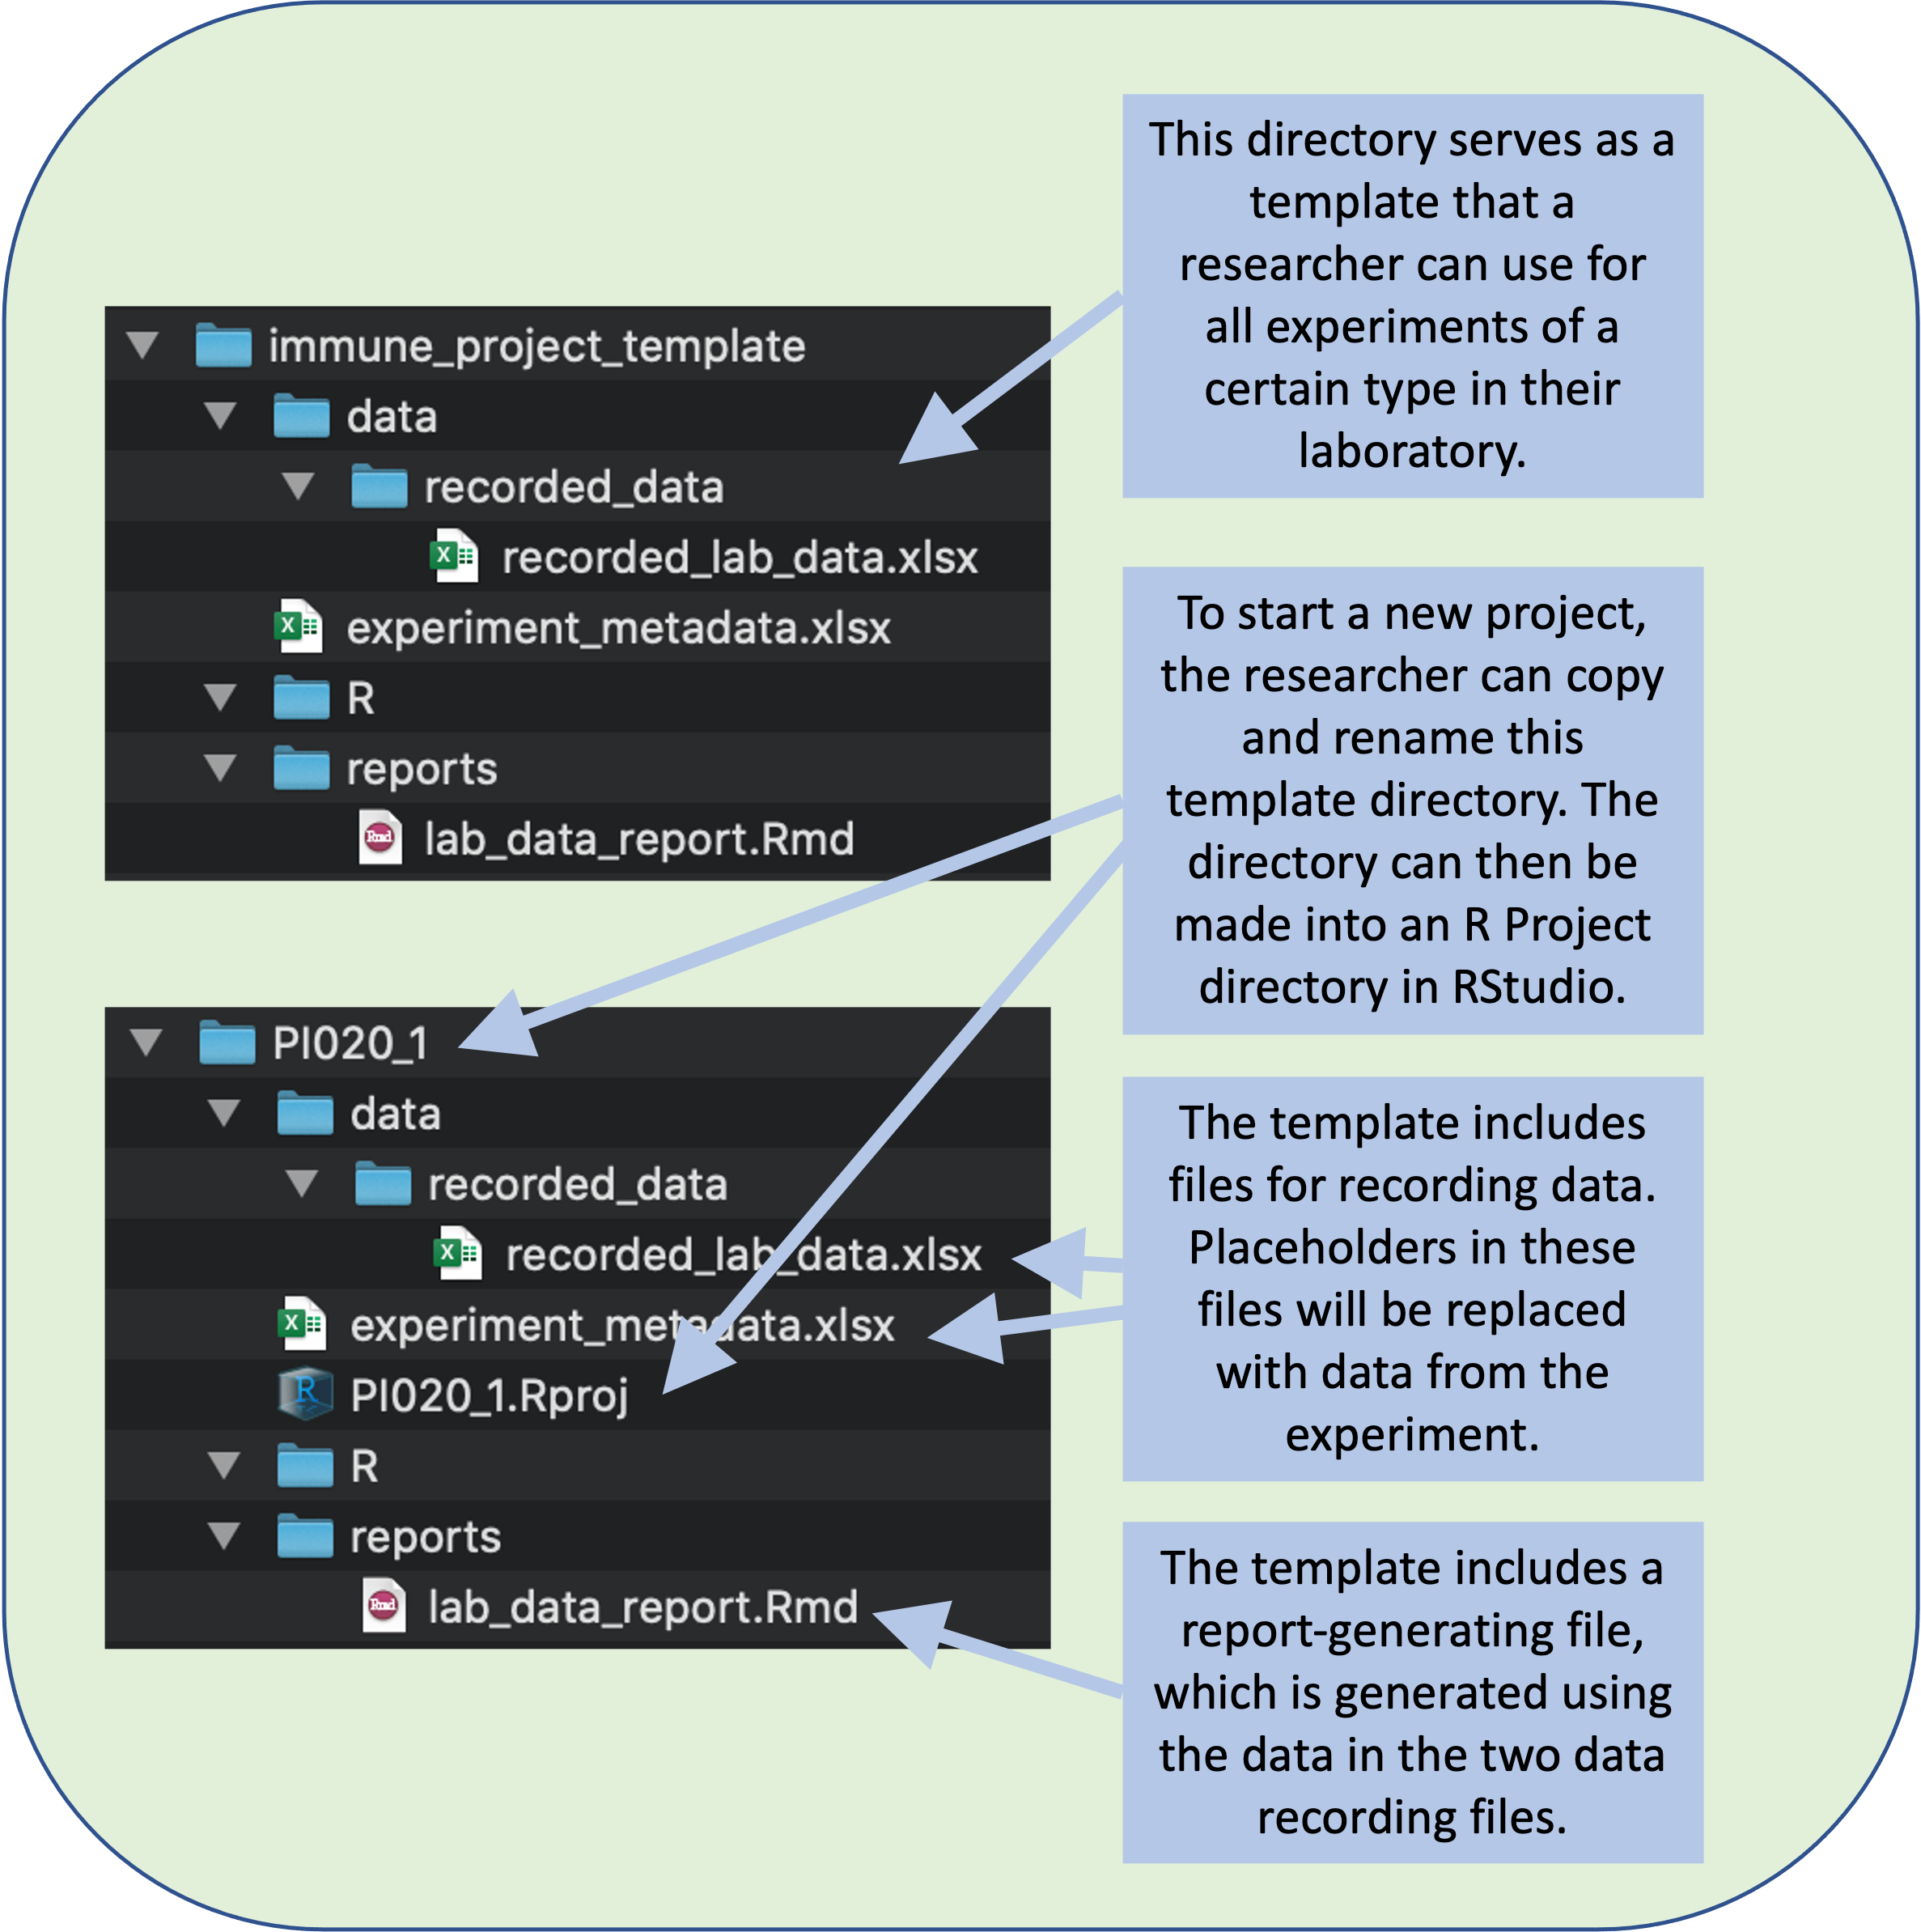
\includegraphics[width=\textwidth]{figures/project_template_directory} \caption[A research group can create a file directory that will serve as a template for all the experiments of a certain type in your laboratory]{A research group can create a file directory that will serve as a template for all the experiments of a certain type in your laboratory. The template can include templates of files for data recording and for generating reports. To start recording data for a new experiment, a researcher can copy and rename this template directory.}\label{fig:templatedirectory}
\end{figure}

This template is not restrictive---it serves as a starting point, but it can
be adapted for each specific project. For example, if you are collecting
data from an assay that you have not used in past experiments, you can add
a new data subdirectory to your project directory to use for storing that new
type of data. Figure \ref{fig:projecttemplatecomplex} shows an example of
how you could customize the basic template shown in Figure \ref{fig:templatedirectory}.

\begin{figure}
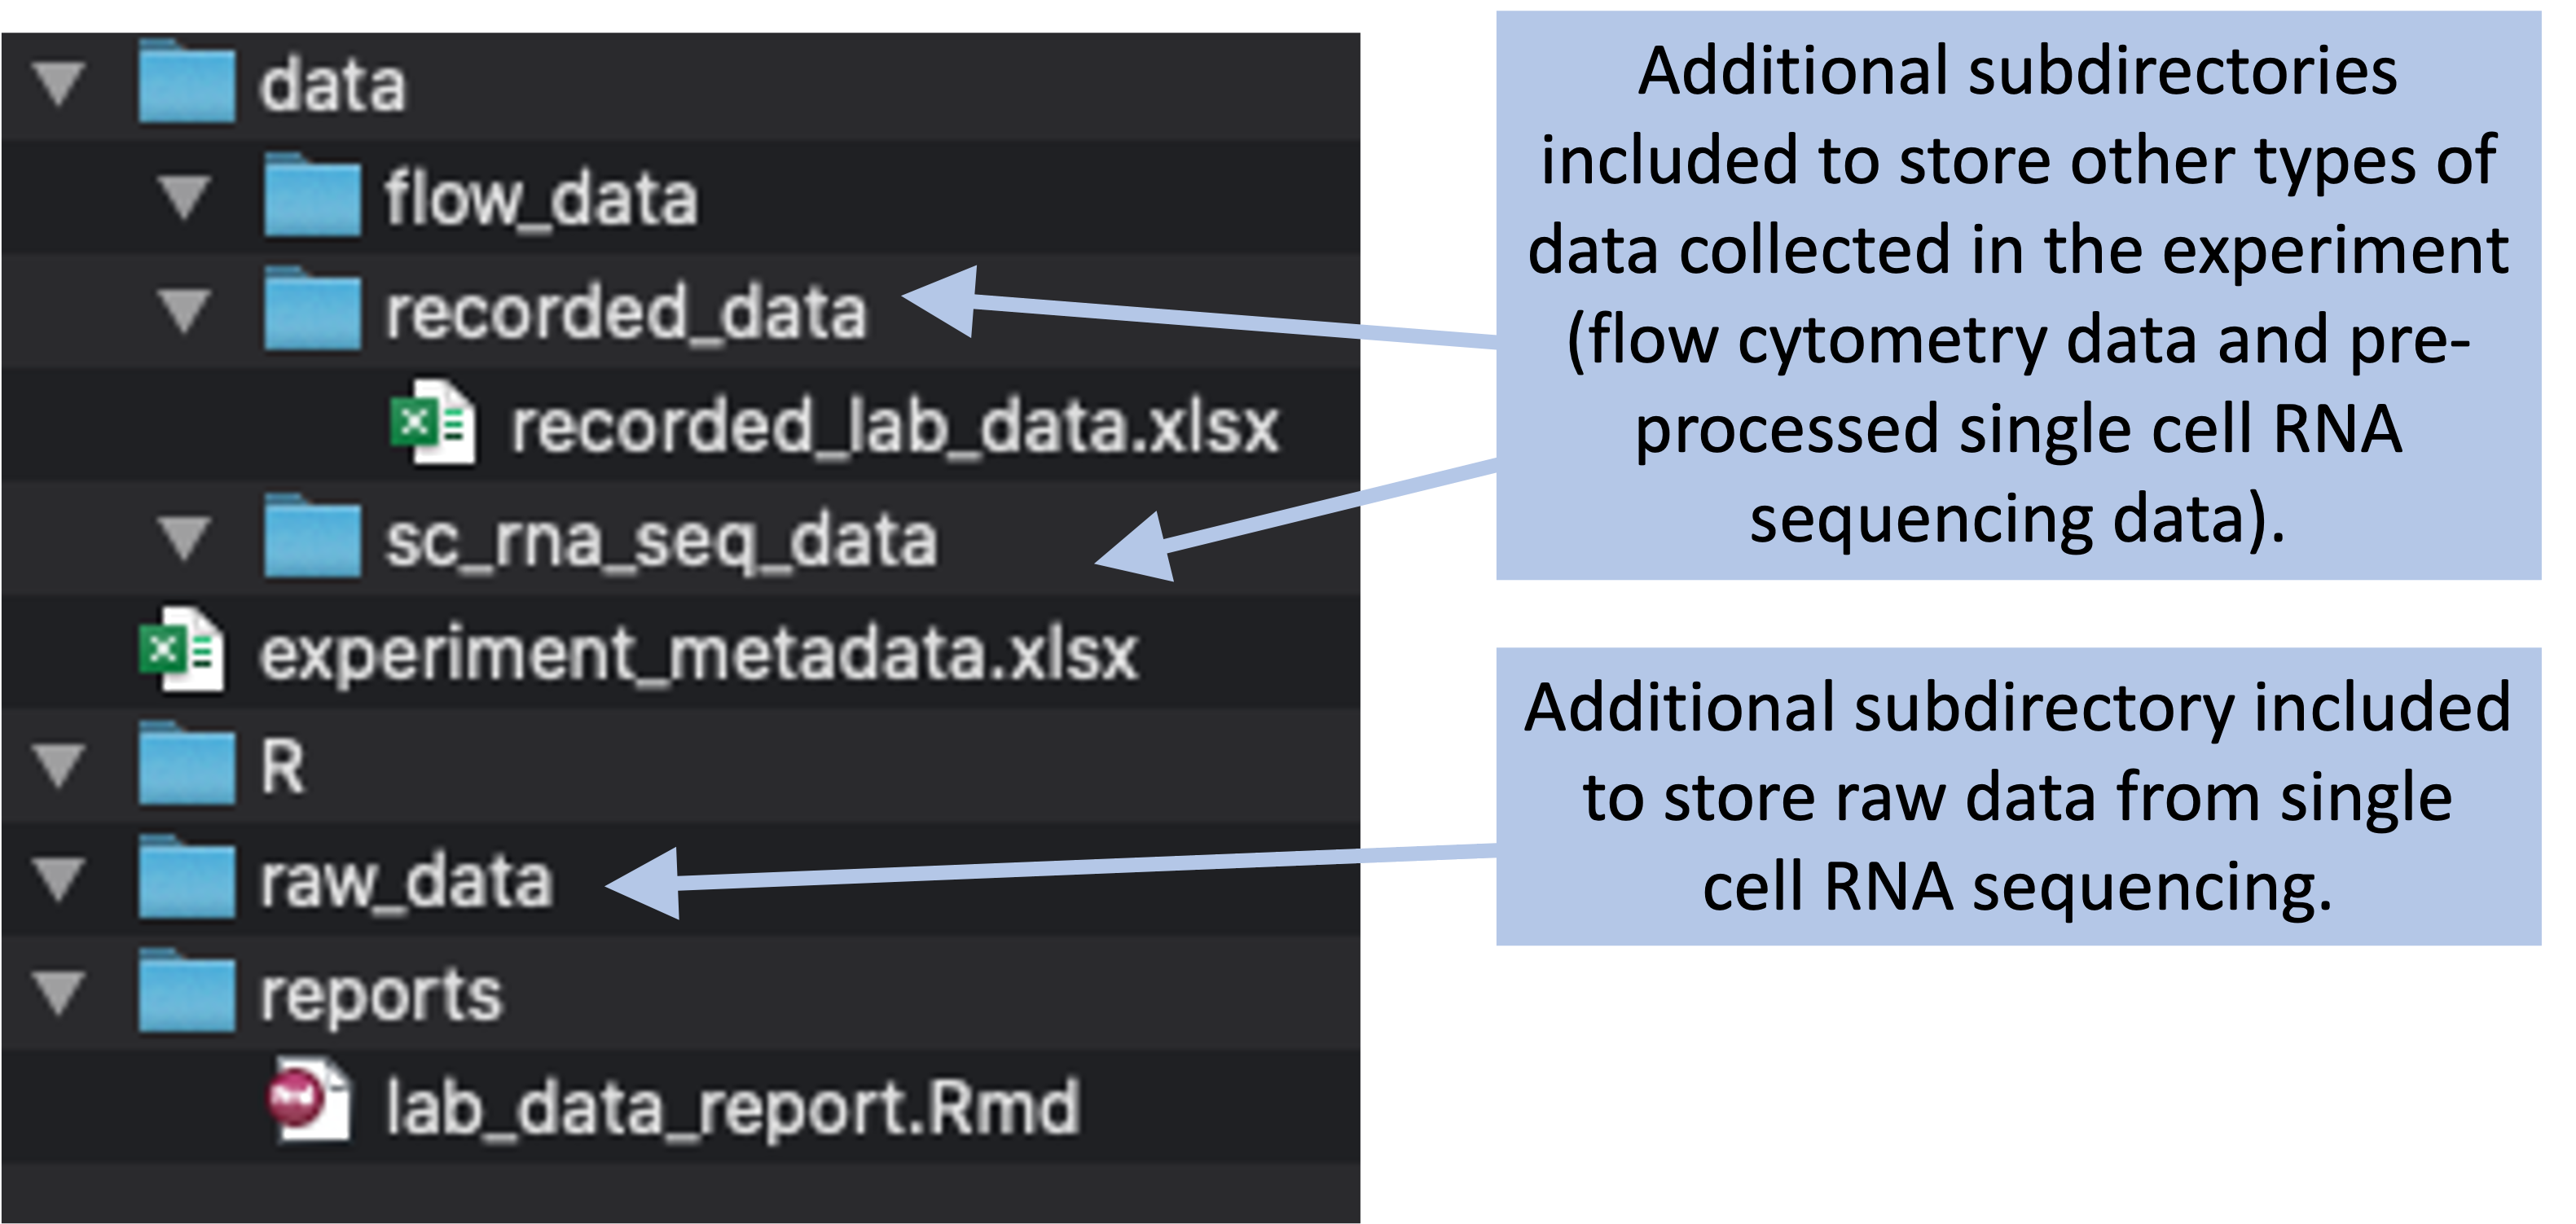
\includegraphics[width=\textwidth]{figures/project_template_morecomplex} \caption[Example of a more complex project directory structure that could be created, with directories added to store data collected through flow cytometry and single cell RNA sequencing]{Example of a more complex project directory structure that could be created, with directories added to store data collected through flow cytometry and single cell RNA sequencing.}\label{fig:projecttemplatecomplex}
\end{figure}

Keep in mind, though, that you do want to keep a balance, where you avoid
unneeded changes to the project template within each specific project's
directory. This is because many of the benefits of standardizing (e.g.,
knowing where things are, building tools that leverage the standardized
directory structure) are lost as the directories for specific projects grow
to be more and more different from each other.

Figure \ref{fig:basicprojecttemplateuse} gives a basic walk-through of the
simple steps you'll use to start a new project directory once you've created
this type of template (we will cover this example in much more detail in the
next module, where we walk through a full example of designing and using a
project template).

\begin{figure*}
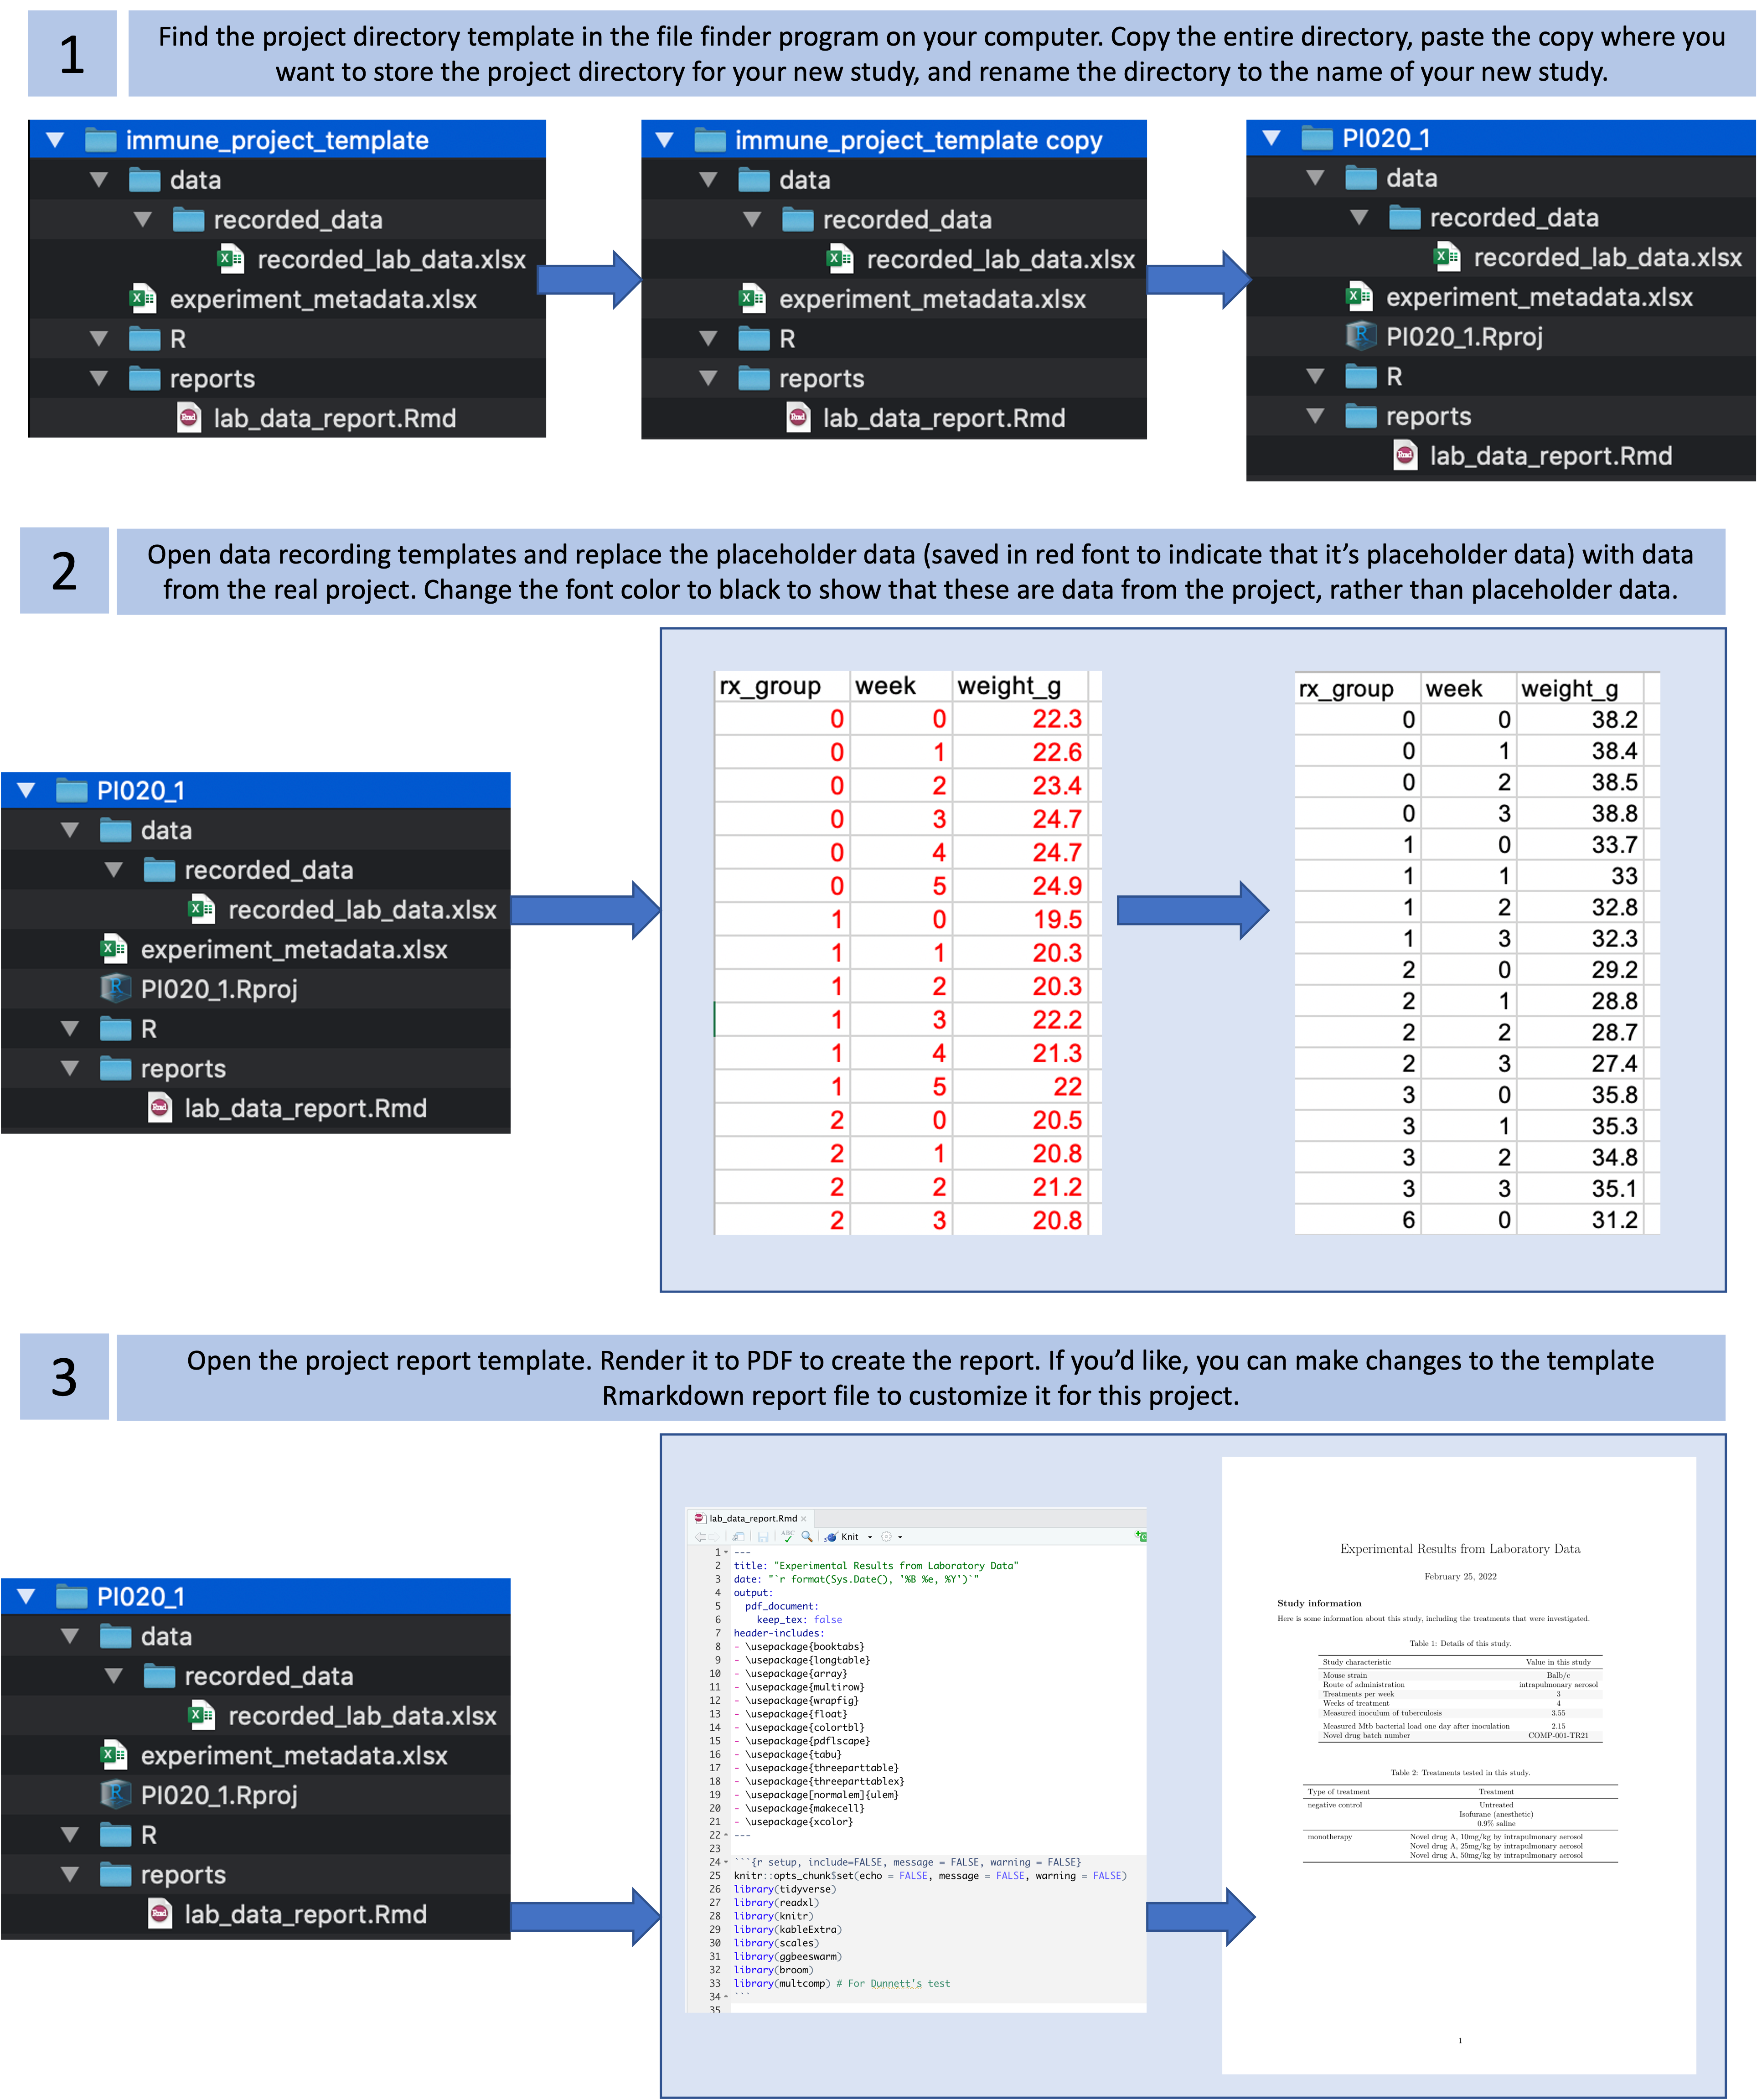
\includegraphics[width=\textwidth]{figures/project_template_basic_use} \caption[Steps in using a basic project directory template that you have created for a type of study or experiment]{Steps in using a basic project directory template that you have created for a type of study or experiment.}\label{fig:basicprojecttemplateuse}
\end{figure*}

\subsection{Project directories as RStudio Projects}\label{project-directories-as-rstudio-projects}

If you are using the R programming language for data pre-processing, analysis,
and visualization---as well as RMarkdown for writing reports and
presentations---then you can use RStudio's ``Project'' functionality to make it
even more convenient to work with files within a research project's directory.
You can make any file directory a ``Project'' in RStudio by chosing ``File'' -\textgreater{}
``New Project'' in RStudio's menu. This gives you the option to create a
project from scratch or to make an existing directory and RStudio Project.

When you make a file directory an RStudio Project, it doesn't change much in
the directory itself except adding a ``.RProj'' file. This file keeps track of
some things about the file directory for RStudio, including preferred settings
for RStudio to use when working in that project.

When you are working in an RStudio Project, RStudio will automatically move your
working directory to be the top-level directory of the Project directory. This
makes it easy to write code that uses this directory as the presumed working
directory, using relative file paths to identify and files within the directory.
We discussed the value of using relative pathnames earlier in this module, when
we discussed how to design file naming conventions for your project directory.
In particular, if you share the project directory with someone else, they can
similarly open the RStudio Project in their own version of RStudio, and all the
relative pathnames to files should work on their system without any problems.
This feature helps make code in an RStudio Project directory reproducible across
different people's computers.

There are some other advantages, as well, to turning each of your research
project directories into RStudio Projects. One is that it is very easy to
connect each of these Projects with GitHub, which facilitates collaborative work
on the project across multiple team members while tracking all changes under
version control. If you are tracking the project directory under the Git version
control system, then when you open the RStudio Project, there will be a special
tab in one of the panes to help in using Git with the project. This tab provides
a visual interface for you to commit changes you've made, so they are tracked
and can be reversed if needed, and also so you can easily push and pull these
committed changes to and from a remote repository, like a GitHub repository, if
you are collaborating with others. This functionality is described in modules
2.9 through 2.11.

Having your project directories set up as R Projects also makes it easy to
navigate among different projects. When you close RStudio and reopen it, it will
automatically open in the last Project you had open. There is a small tab in the
top right hand corner of the RStudio window that lists the project you are
currently in. To move to a different Project, you can click on the down arrow
beside this project name. There will be a list of your most recent projects, as
well as options to open any Project on your computer. If you want to work in
RStudio, but not in any of the Projects, you can choose to ``Close Project''.

\section{Example: Creating a project template}\label{module8}

For this module, we'll show an example of creating a project directory template
for a lab group. We will walk through the process of creating a project
directory template that could be used to manage and analyze data from any of the
specific studies for this group. We'll start by discussing the steps of the
conceptual design---figuring out how a blueprint for the standard subdirectories
and the file naming conventions. We'll then show how this blueprint can be
developed into physical implementation: a file directory that can be copied and
renamed to initiate a new project. The full directory of files for this example
can be found at \url{https://github.com/geanders/example_for_improve_repro}, where you
can download them or explore them online.

\textbf{Objectives.} After this module, the trainee will be able to:

\begin{itemize}
\tightlist
\item
  Examine files from previous projects as a step in developing a project
  directory template
\item
  Develop a structure of subdirectories for a project directory template
\item
  Create a project directory template to initialize consistently-formatted
  directories for a lab group's experiments
\item
  Explain how a report template can be incorporated within a project directory
  template
\end{itemize}

\subsection{Description of the example set of studies}\label{description-of-the-example-set-of-studies}

In this module, we'll use an example based on a set of real immunology
experiments. This example highlights how a research laboratory will often
conduct a similar type of experiment many times, so it lets us demonstrate how a
project directory template can be reused across similar experiments. It will
allow us to show you how you can move from designing a file directory for a
single experiment to designing one that can be used repeatedly, and then how you
can take advantage of consistency in the directory structure across projects to
make templates for data collection that can be reused.

This example covers a group of studies that explored novel
treatments for tuberculosis. While treatments exist for tuberculosis, the
current treatment regime is lengthy and involves a combination of multiple
drugs. If the treatment is not completed, it can result in the development and
spread of drug-resistant tuberculosis strains, and so the treatment sometimes
must be done under observation \citep{barry2009new}. If the patient has a
strain of tuberculosis that is resistant to first-line drugs, they
need to be treated with second-line drugs, which can have serious side effects
\citep{barry2009new}. There is a critical need to develop more candidate drugs
against this disease, given all the limitations and struggles of the current
treatment regime.

Each study investigates how mice challenged with tuberculosis respond
to different treatments, both in terms of how well they handle the treatment
(assessed by checking if their weight decreases notably while on treatment) and
also how well the treatment manages to limit the growth of tuberculosis in the
mouse's lungs.

These example studies were conducted with similar designs and similar
goals---all aimed to test candidate treatments for tuberculosis. Most studies in
this set tested one or more treatments as well as one or more controls. The
controls could include negative controls, like saline solution, or positive
controls, like a drug already in use to treat the disease (e.g., isoniazid). A
few of the studies tested only controls, to develop baseline expectations for
things like the bacterial load in different mouse strains. The set of studies
tested some treatments that were monotherapies (only one drug given to the
animal) as well as some that were combinations of two or three drugs.
For many of the drugs that were tested, they were tested at different doses and,
in some cases, different methods of delivery or different mouse models.

Each of the treatments were given to several mice that had been infected with
\emph{Mycobacterium tuberculosis}. During the treatment, the mice were weighed
regularly. This weight measurement helps to determine if a particular treatment
is well-tolerated by the animals---if not, it may show through the treated mice
losing weight during treatment. For convenience, the mice were not weighed
individually. Instead, mice with the same treatment were kept in a single cage,
and the entire cage was weighed, the weight of the cage itself factored out, and
the average weight of mice determined by dividing by the number of mice in the
cage. After a period of time, the mice were sacrificed and one lobe from their
lungs was used to determine each mouse's bacterial load, through plating the
material from the lobe and counting the colony forming units (CFUs). One aim of
the data analysis is to compare the bacterial load of mice under various
treatments to the bacterial load of mice in the control group.

The full set of studies included 19 studies. These were conducted at
different times, but the data for all of the studies can be collected using a
common format, and we'll talk about how both data collection templates and a
project directory template could be designed to accomodate these experiments.

\subsection{Step 1: Survey of data collected for the projects}\label{step-1-survey-of-data-collected-for-the-projects}

The first step in developing a project template is to survey the typical types
of files that are included in your research projects. To give an example of this
part of the design process, let's walk through the types of data that were
collected for the example studies.

First, there were metadata recorded for each study. Figure
\ref{fig:metadata} gives an example. This includes information about the strain
of mouse that was used in the study, treatment details (including the method of
giving the drug or drugs, how often they were given each week, and for how many
weeks), how much bacteria the animals were exposed to (measured both in terms of
the inoculum they were given and their bacterial load one day after they were
given that inoculum, which was based on sacrificing one animal the day after
challenging all the animals with the bacteria), and, if the study included a
novel drug as part of the tested treatment, the batch number of that drug.

\begin{figure*}
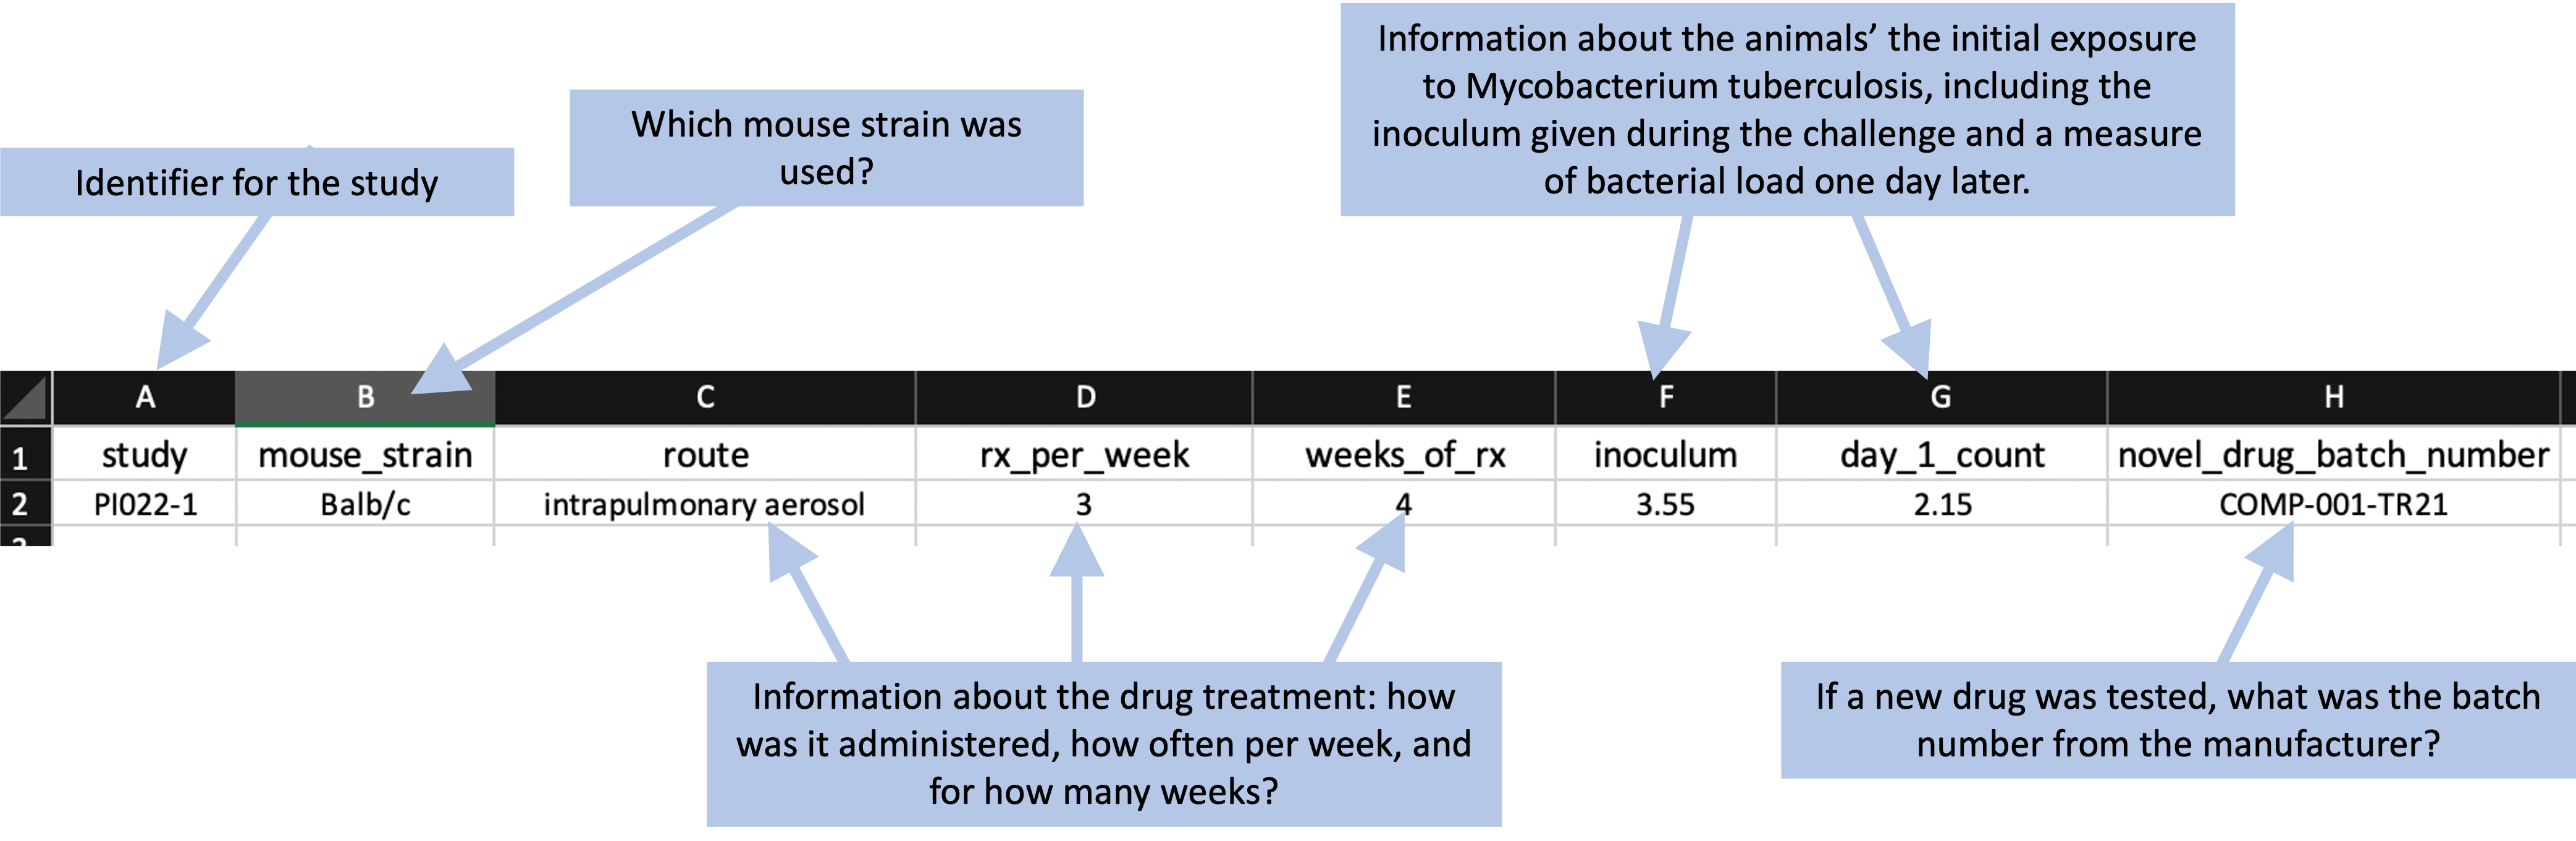
\includegraphics[width=\textwidth]{figures/project_metadata} \caption[Example of recording metadata for a study in the set of example studies for this module]{Example of recording metadata for a study in the set of example studies for this module.}\label{fig:metadata}
\end{figure*}

Next, the researchers recorded some information about each treatment group
within the experiment. This typically included at least one negative control. In
some cases, there was also a positive control, in which the animals were treated
with a drug that's in standard use against tuberculosis already (e.g.,
isoniazid). Most studies would also test one or more treatments, which could
include monotherapies or combined therapies. Figure \ref{fig:treatmentdetails}
shows an example of the data that were recorded on each treatment in the study.
These data include the names and doses of up to three drugs in each treatment,
as well as a column where the researcher can provide detailed specifications of
the treatment.

\begin{figure*}
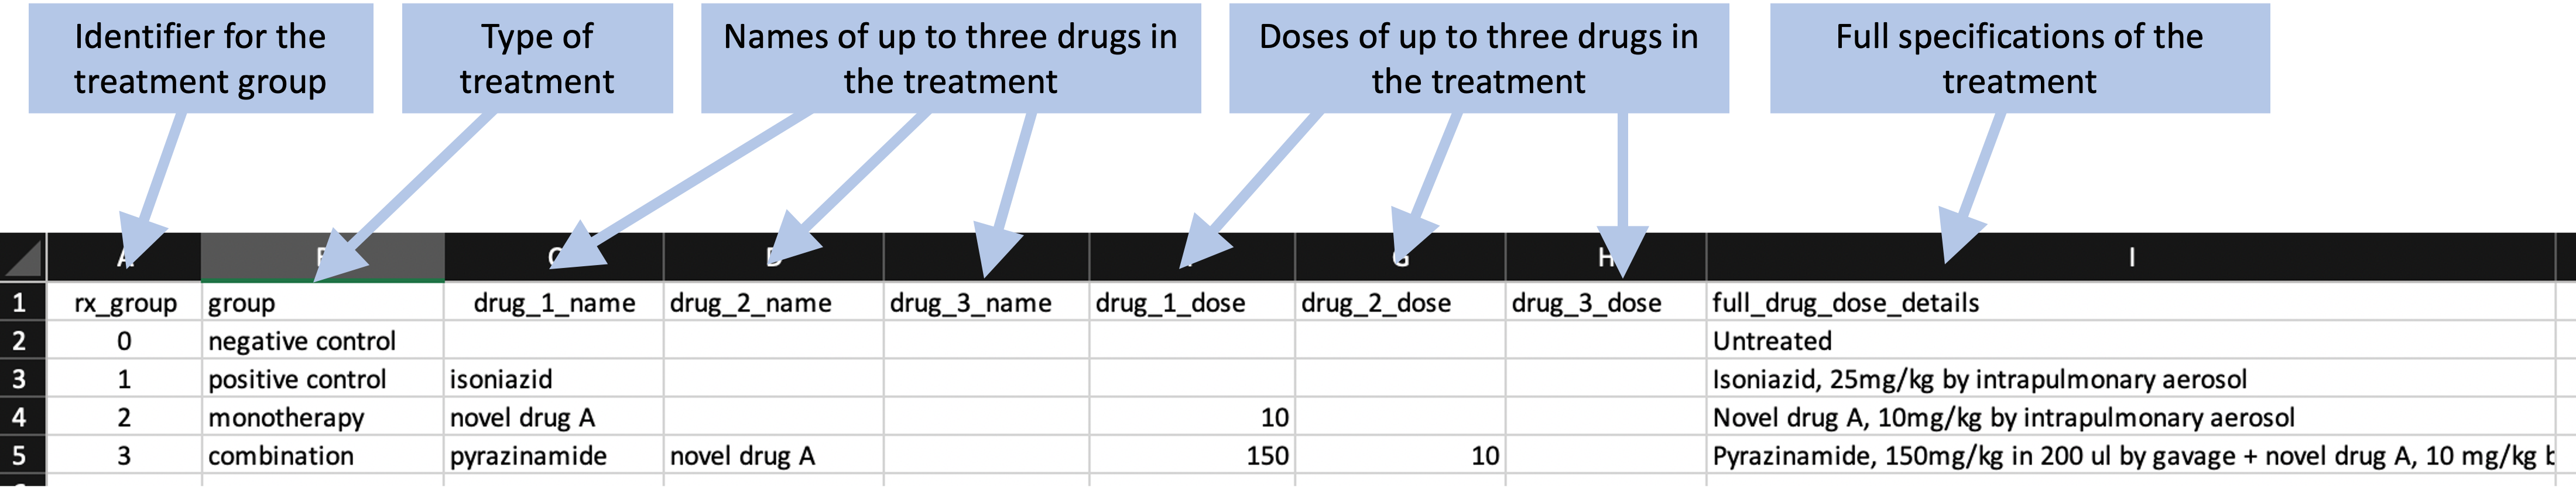
\includegraphics[width=\textwidth]{figures/project_treatment_details} \caption[Example of recording treatment details for a study in the set of example studies for this module]{Example of recording treatment details for a study in the set of example studies for this module.}\label{fig:treatmentdetails}
\end{figure*}

Once the animals were challenged with the bacteria, treatment began, and two
main types of data were measured and recorded. First, the mice were weighed once
a week. For convenience, the mice were not weighed
individually. Instead, mice with the same treatment were kept in a single cage,
and the entire cage was weighed, the weight of the cage itself factored out, and
the average weight of mice for that treatment determined by dividing the weight
of all mice in the cage by the number of mice in the cage. These weights were converted to a measure of the percent change in
weight since the start of treatment. If the animals' weights decrease during the
treatment, it is a marker that the treatment is not well-tolerated by the
animals. Figure \ref{fig:mouseweight} shows an example of how these data could be
recorded. All animals within a treatment group were kept in the same cage, and
this cage was measured once a week. By dividing the weight of all animals in the
cage by the number of animals, the researchers could estimate the average weight
of animals in that treatment group, which is recorded as shown in Figure
\ref{fig:mouseweight}.

\begin{figure*}
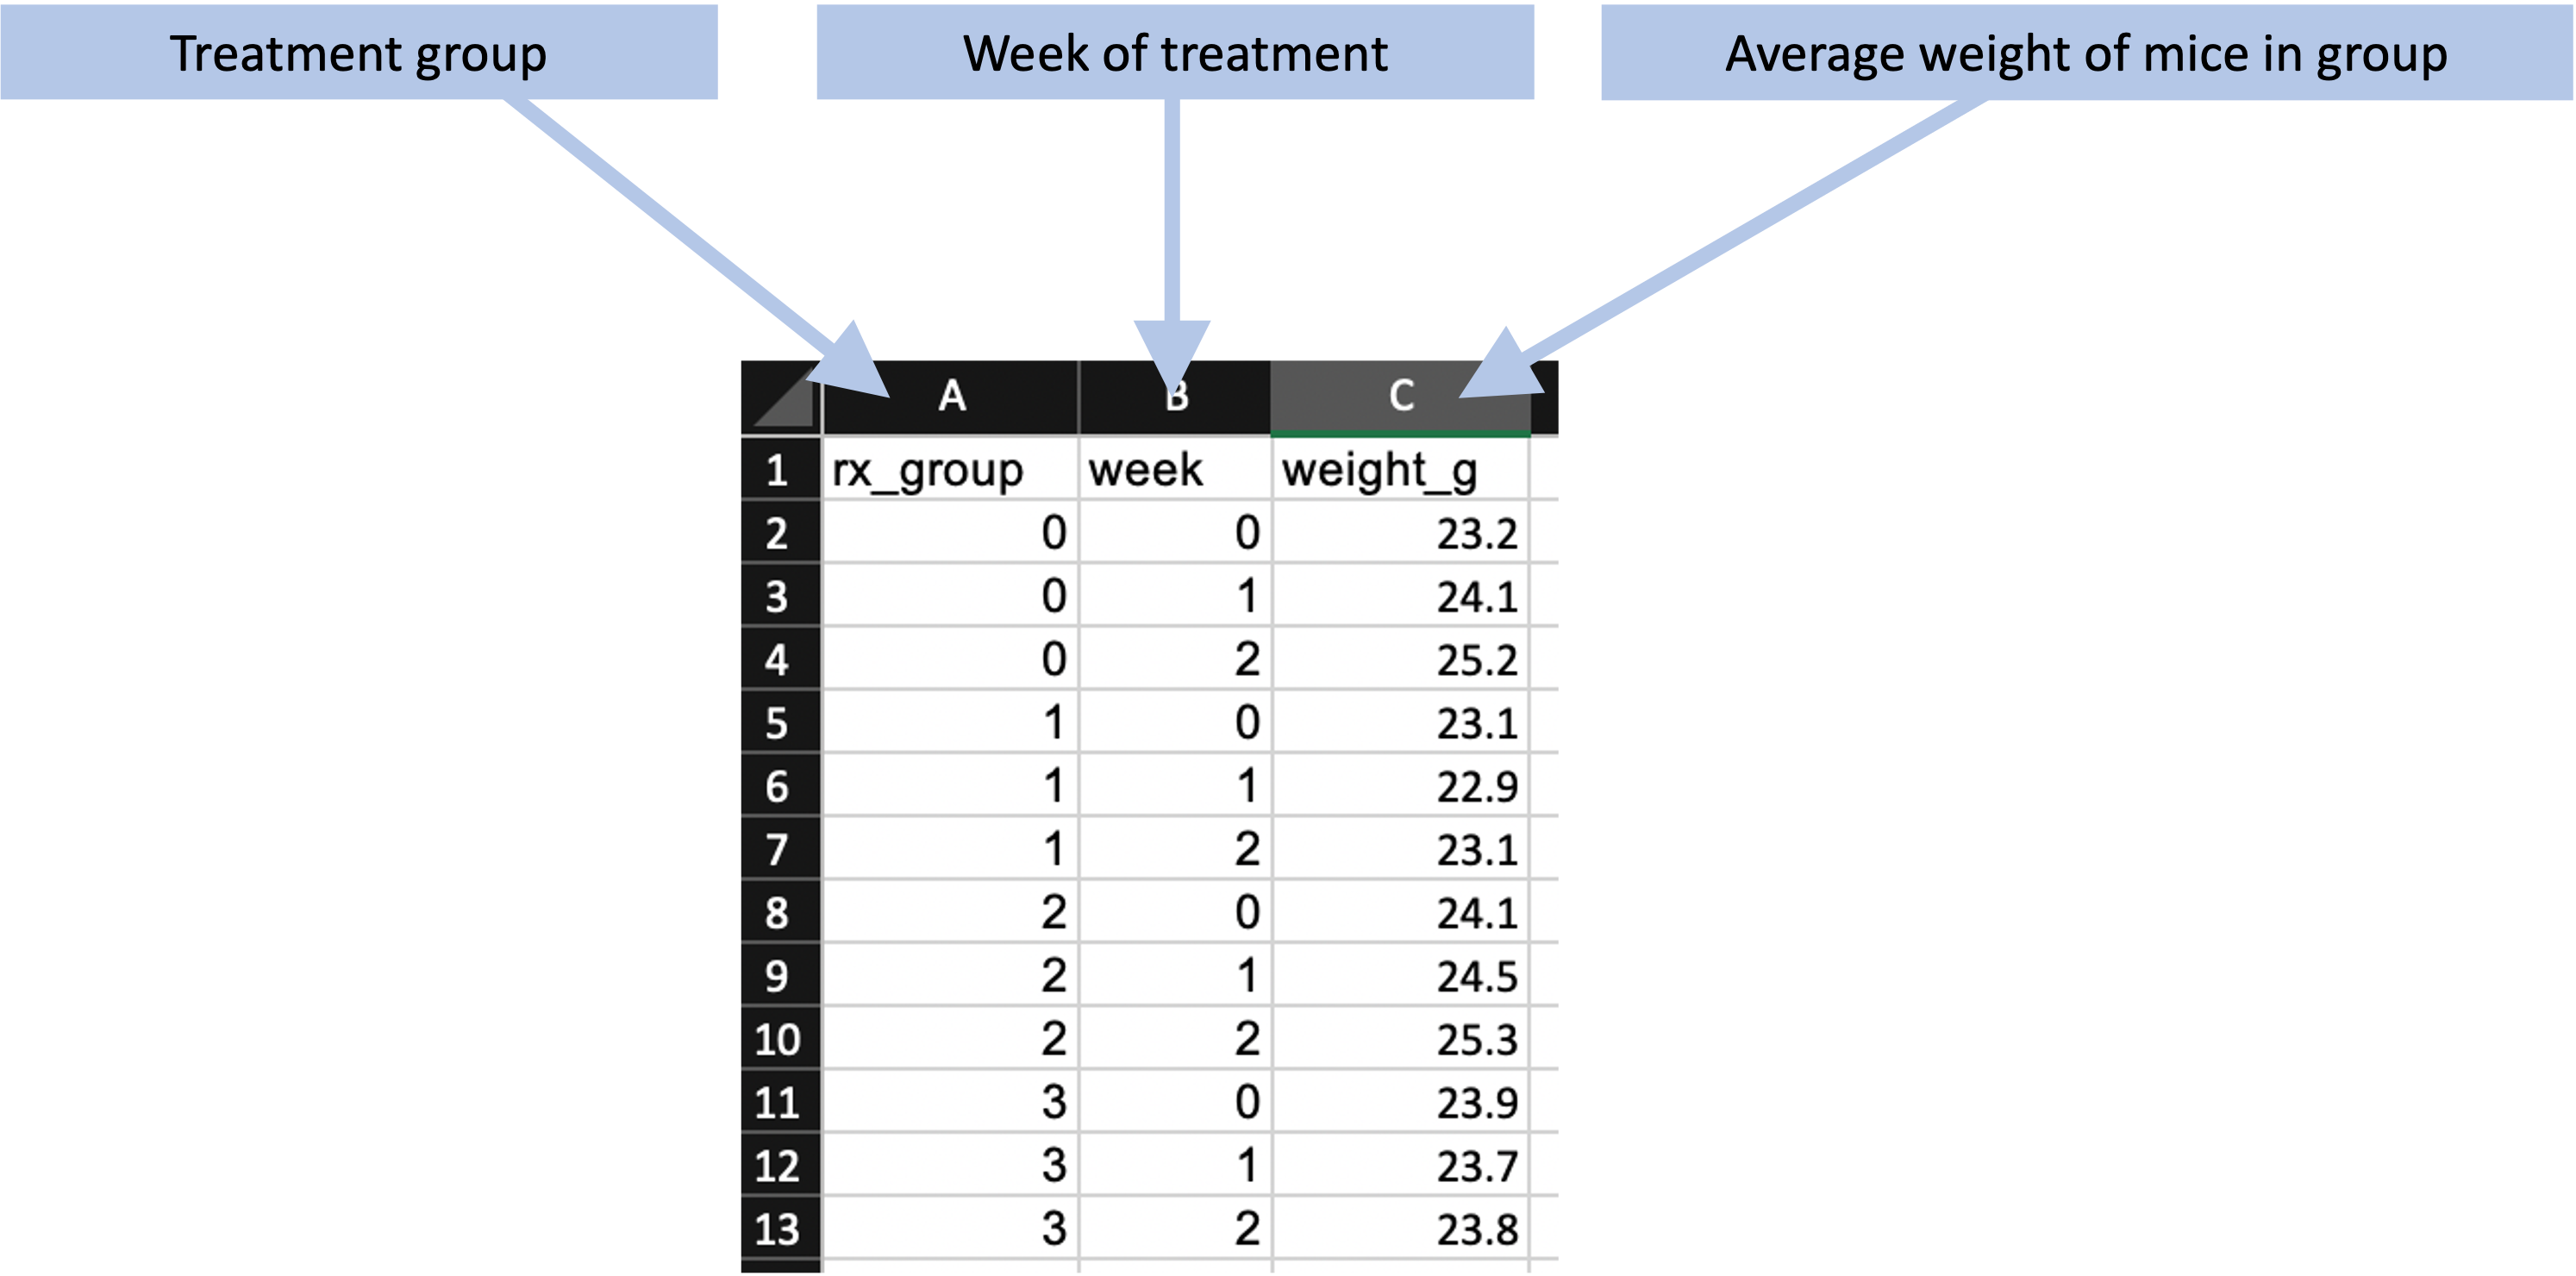
\includegraphics[width=\textwidth]{figures/project_mouse_weights} \caption[Example of recording weekly weights of mice in each treatment group for the example set of studies]{Example of recording weekly weights of mice in each treatment group for the example set of studies.}\label{fig:mouseweight}
\end{figure*}

Finally, after the treatment period, the mice were sacrificed and a portion of
each mouse's lung was used to estimate the bacterial load in that mouse. Figure
\ref{fig:bacterialload} shows an example of how the data on the bacterial load
in each mouse can be recorded.

\begin{figure*}
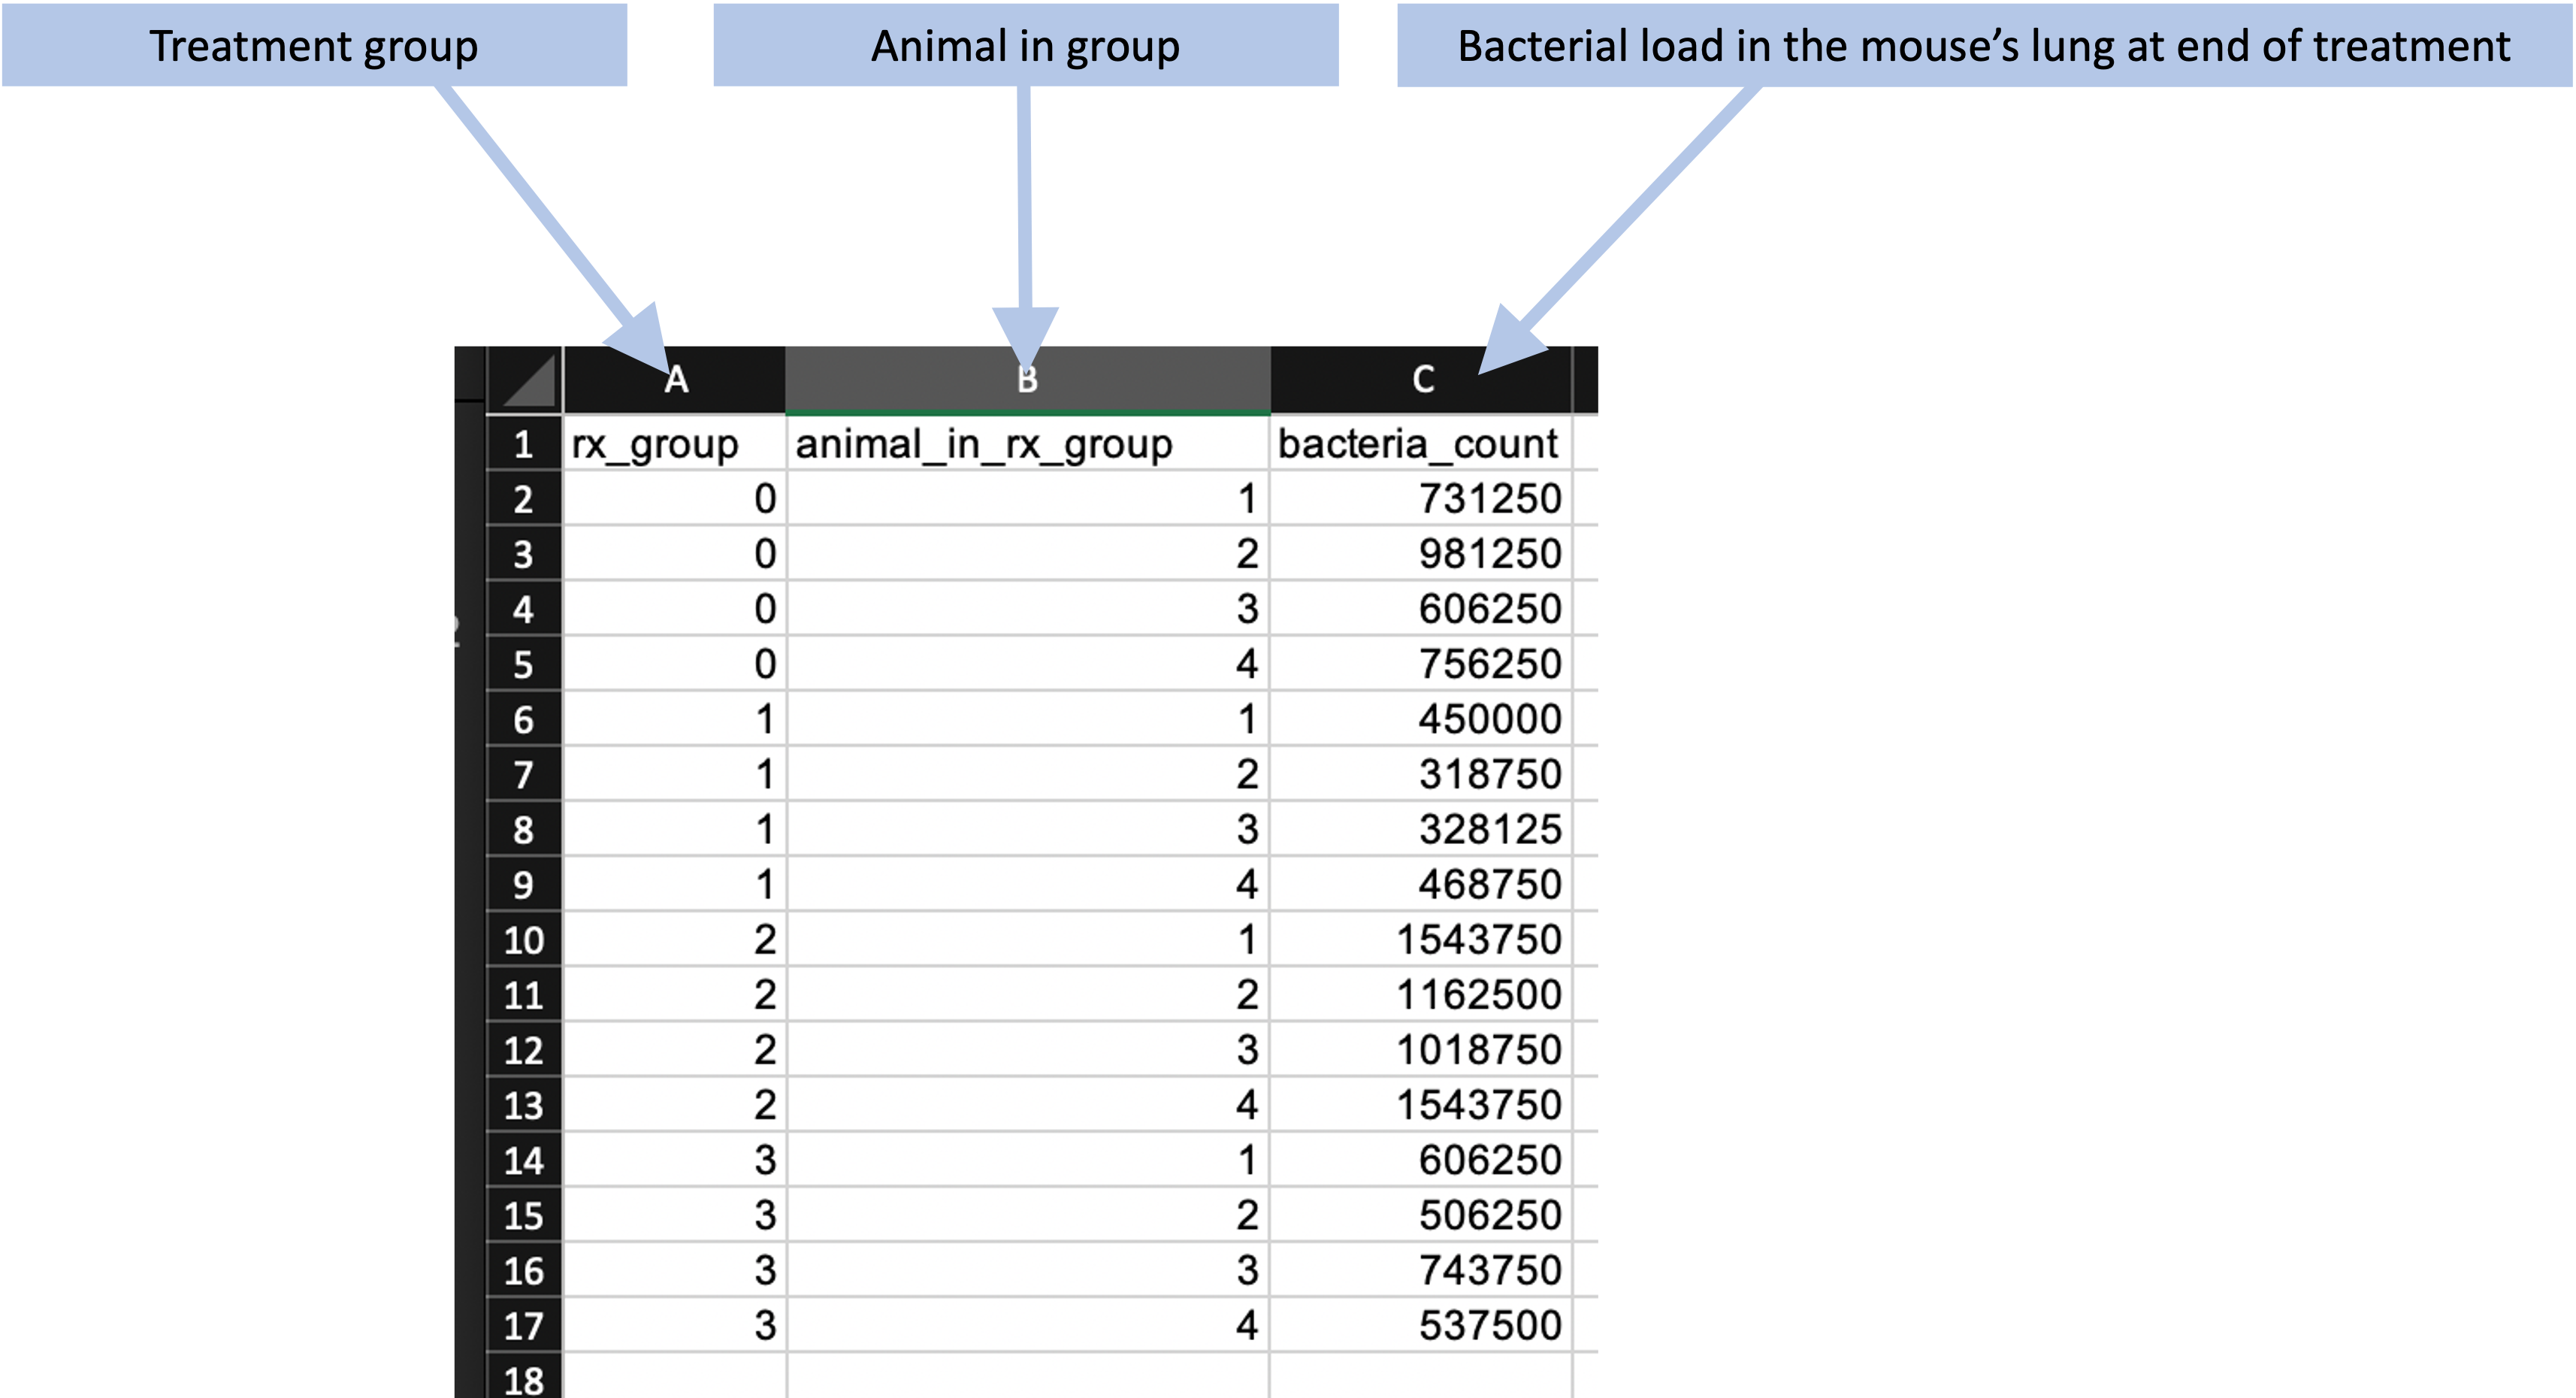
\includegraphics[width=\textwidth]{figures/project_bacterial_load} \caption[Example of recording the bacterial load in the lungs of each mouse at the end of treatment for the example set of studies]{Example of recording the bacterial load in the lungs of each mouse at the end of treatment for the example set of studies.}\label{fig:bacterialload}
\end{figure*}

These examples are all data that the researchers record by entering them on
spreadsheets. It is helpful at this stage to ensure this type of data is
recorded in a way that separates data recording and analysis (module 2.1).
The example files we've shown here do---there are no extra elements in these
spreadsheets that do calculations or create graphs. Later in this module, we'll
talk a bit more about how these templates can be designed as part of the
process of designing the full project directory template. Earlier modules
(modules 2.4 and 2.5) provide more focused details on designing data collection
templates like these.

Another type of files that the group's studies typically generate are ones
that are generated directly by laboratory equipment. For example, their
experiments may include flow cytometry assays, with files output in a
specialized format directly from the flow cytometer. Some experiments might
also collect data through single-cell RNA sequencing. We'll want to keep
these files in mind as we design the structure of the project directory
template.

\subsection{Step 2: Organizing a project directory}\label{step-2-organizing-a-project-directory}

Once you've determined the types of files that you'll normally include in your
project, you then need to decide how to organize them into subdirectories in the
project file directory. In this case, we've organized the project directory
template to include just a few things at the top level (Figure
\ref{fig:templatedirectorymod8}, also shown in module 2.7):

\begin{itemize}
\tightlist
\item
  A spreadsheet that stores meta-data about the experiment
\item
  A subdirectory named ``raw\_data'', where we'll store original raw files of
  data, before it is pre-processed, focusing on data generated by laboratory
  equipment
\item
  A subdirectory named ``data'', which will store experimental data once it
  has been pre-processed, as well as recorded data that do not require pre-processing
\item
  A subdirectory named ``R'', which will store code for pre-processing and analysis
\item
  A subdirectory named ``reports'', which will store the files to generate
  reports, as well as any reports that are ultimately generated
\end{itemize}

\begin{figure}
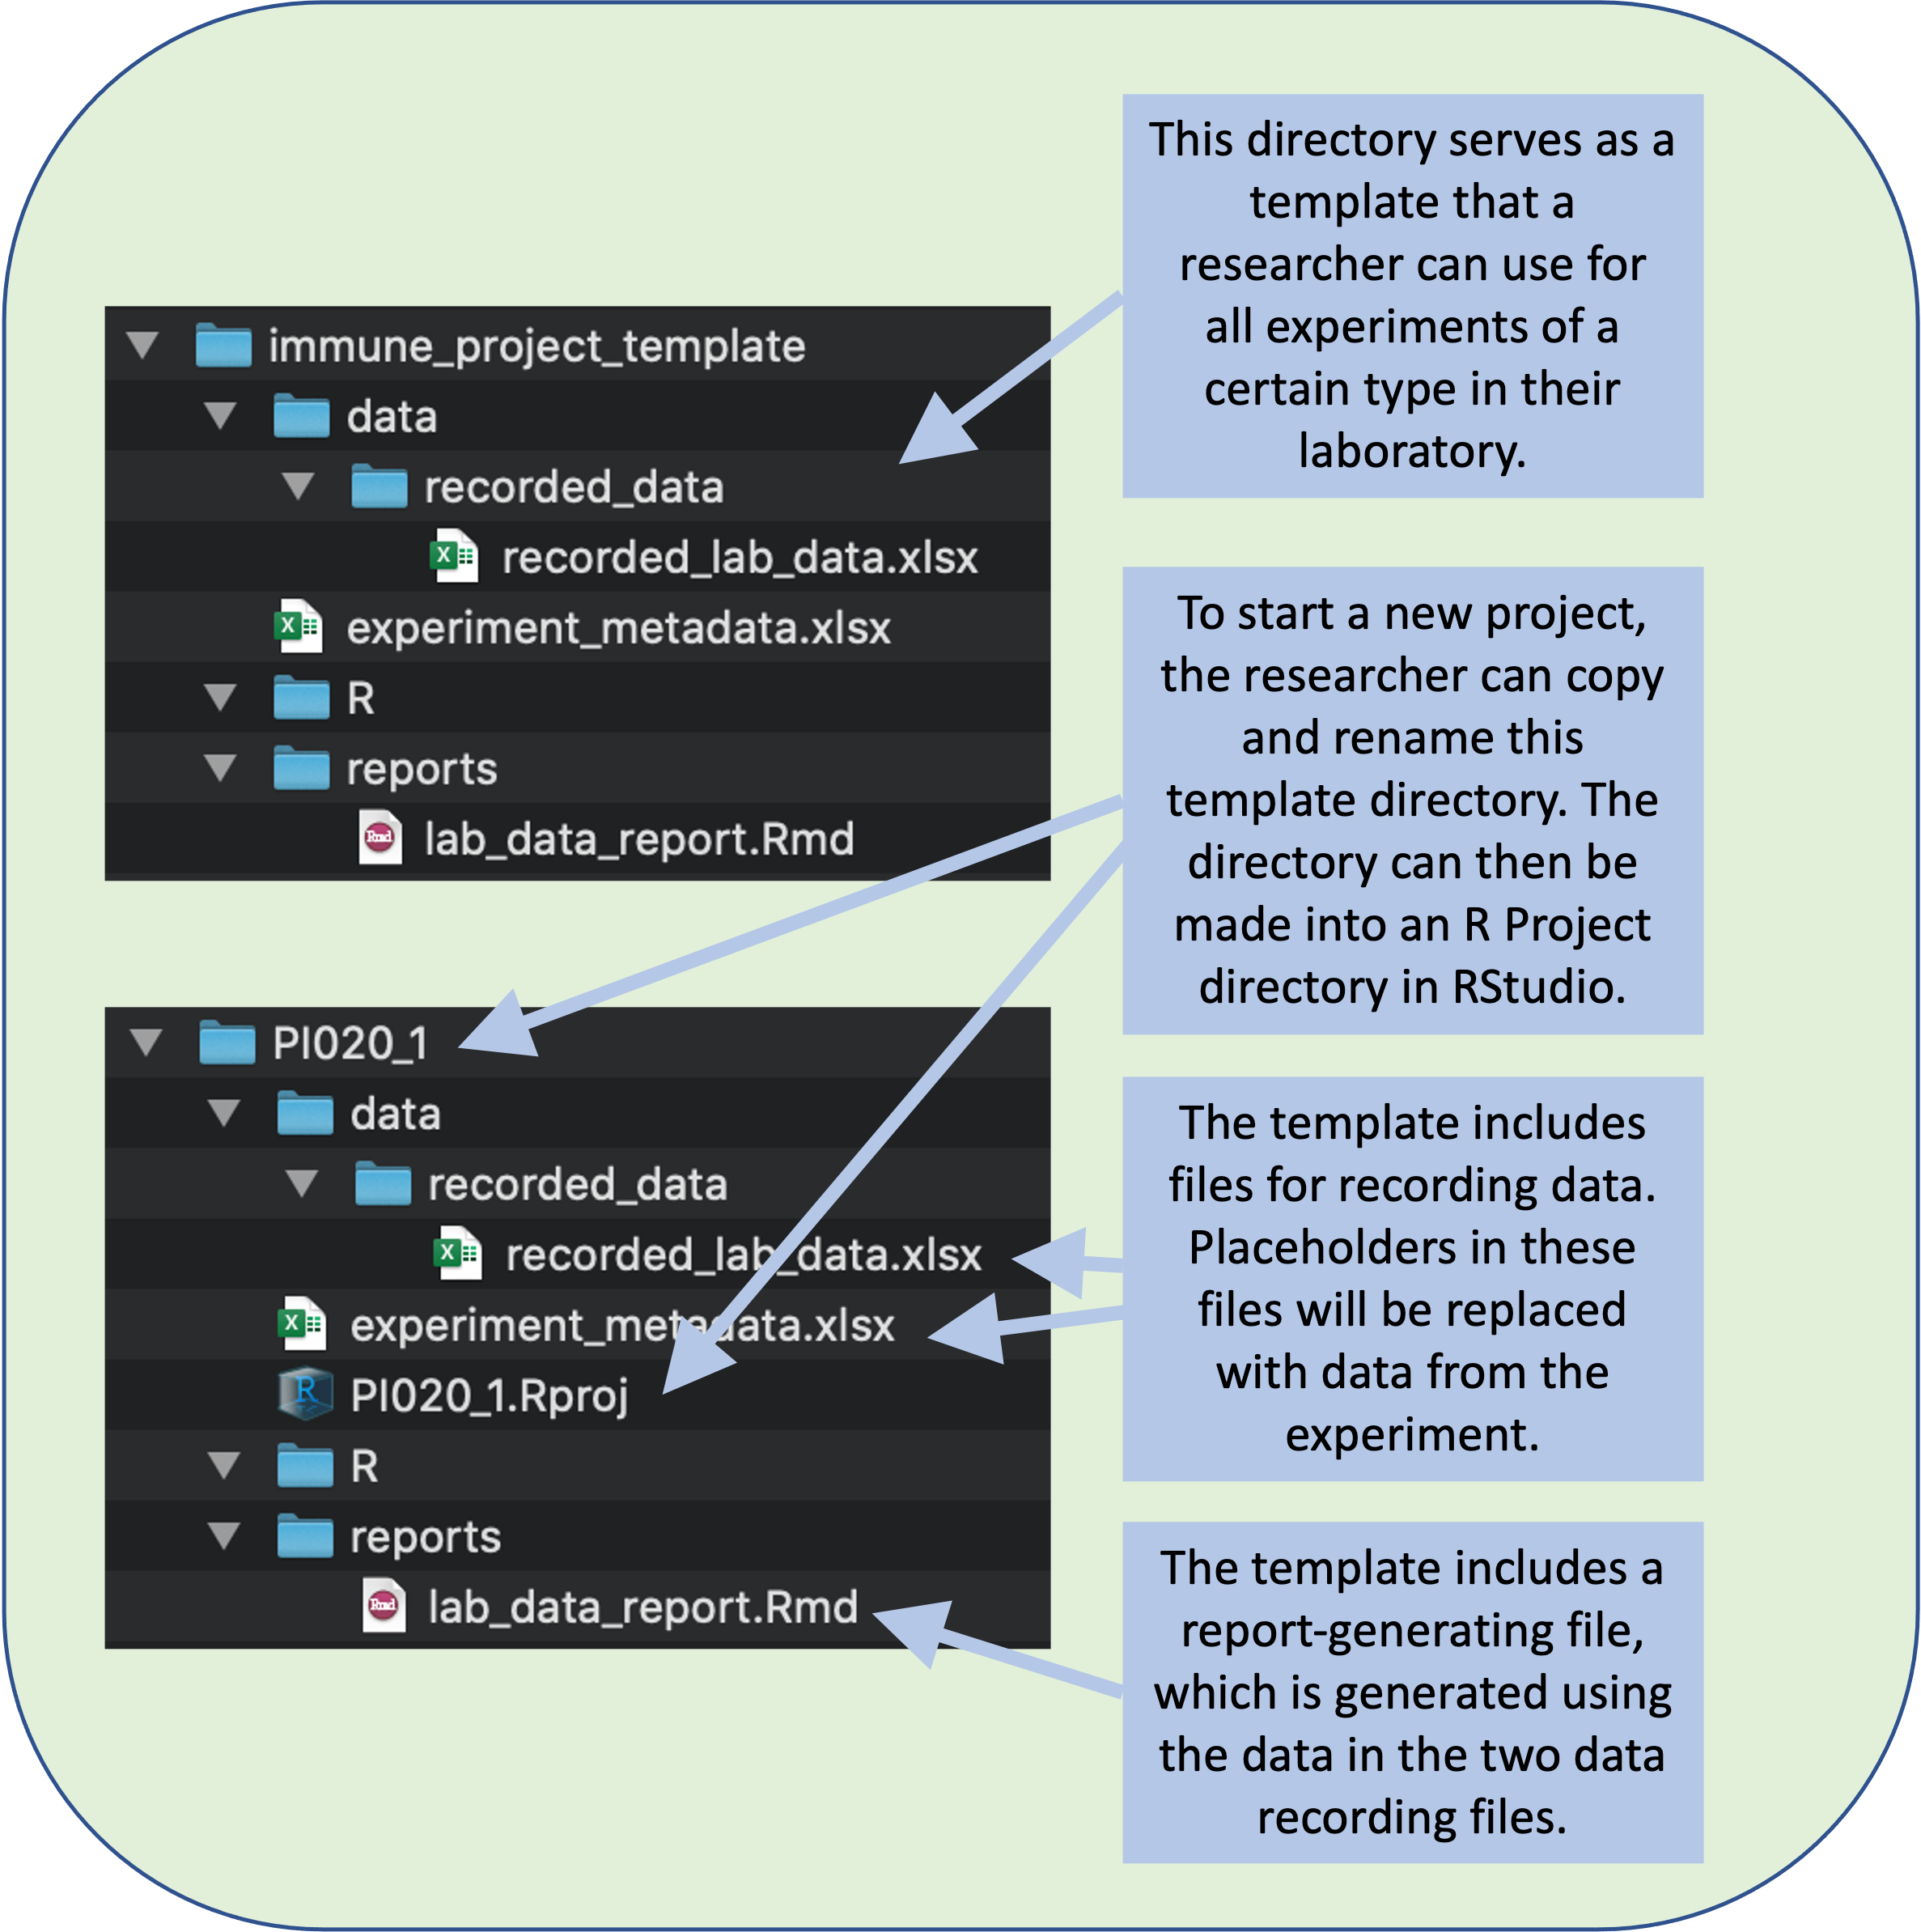
\includegraphics[width=\textwidth]{figures/project_template_directory} \caption[A research group can create a file directory that will serve as a template for all the experiments of a certain type in your laboratory]{A research group can create a file directory that will serve as a template for all the experiments of a certain type in your laboratory. The template can include templates of files for data recording and for generating reports. To start recording data for a new experiment, a researcher can copy and rename this template directory.}\label{fig:templatedirectorymod8}
\end{figure}

You may have noticed that this structure captures each of the main elements
that we discussed including in a project template in the last module:
data, code, reports, and metadata.

In this structure, we've selected subdirectory names that are generic enough
(e.g., ``data'', ``reports'') that they can be reused across many of our projects
without modification. These names should also be clear to any researcher that
explores this directory in the future, since the names are clear and
unambiguous. However, you might make different choices---for example, if
some of your team aren't familiar with R as a programming language, you may
want to use the subdirectory name ``code'' rather than ``R''.

Within some of the subdirectories, we can include more subdirectories to further
organize files (Figure\ref{fig:projecttemplatecomplexmod8}, repeated from
module 2.7). For example, within the ``data'' subdirectory, we can have
subdirectories for different types of data:

\begin{itemize}
\tightlist
\item
  A subdirectory named ``flow\_data'' for data from flow cytometry
\item
  A subdirectory named ``recorded\_data'', for data that are recorded ``by hand''
  in the laboratory (for example, the weights of animals)
\item
  A subdirectory named ``sc\_rna\_seq\_data'' for data from single-cell RNA
  sequencing
\end{itemize}

\begin{figure}
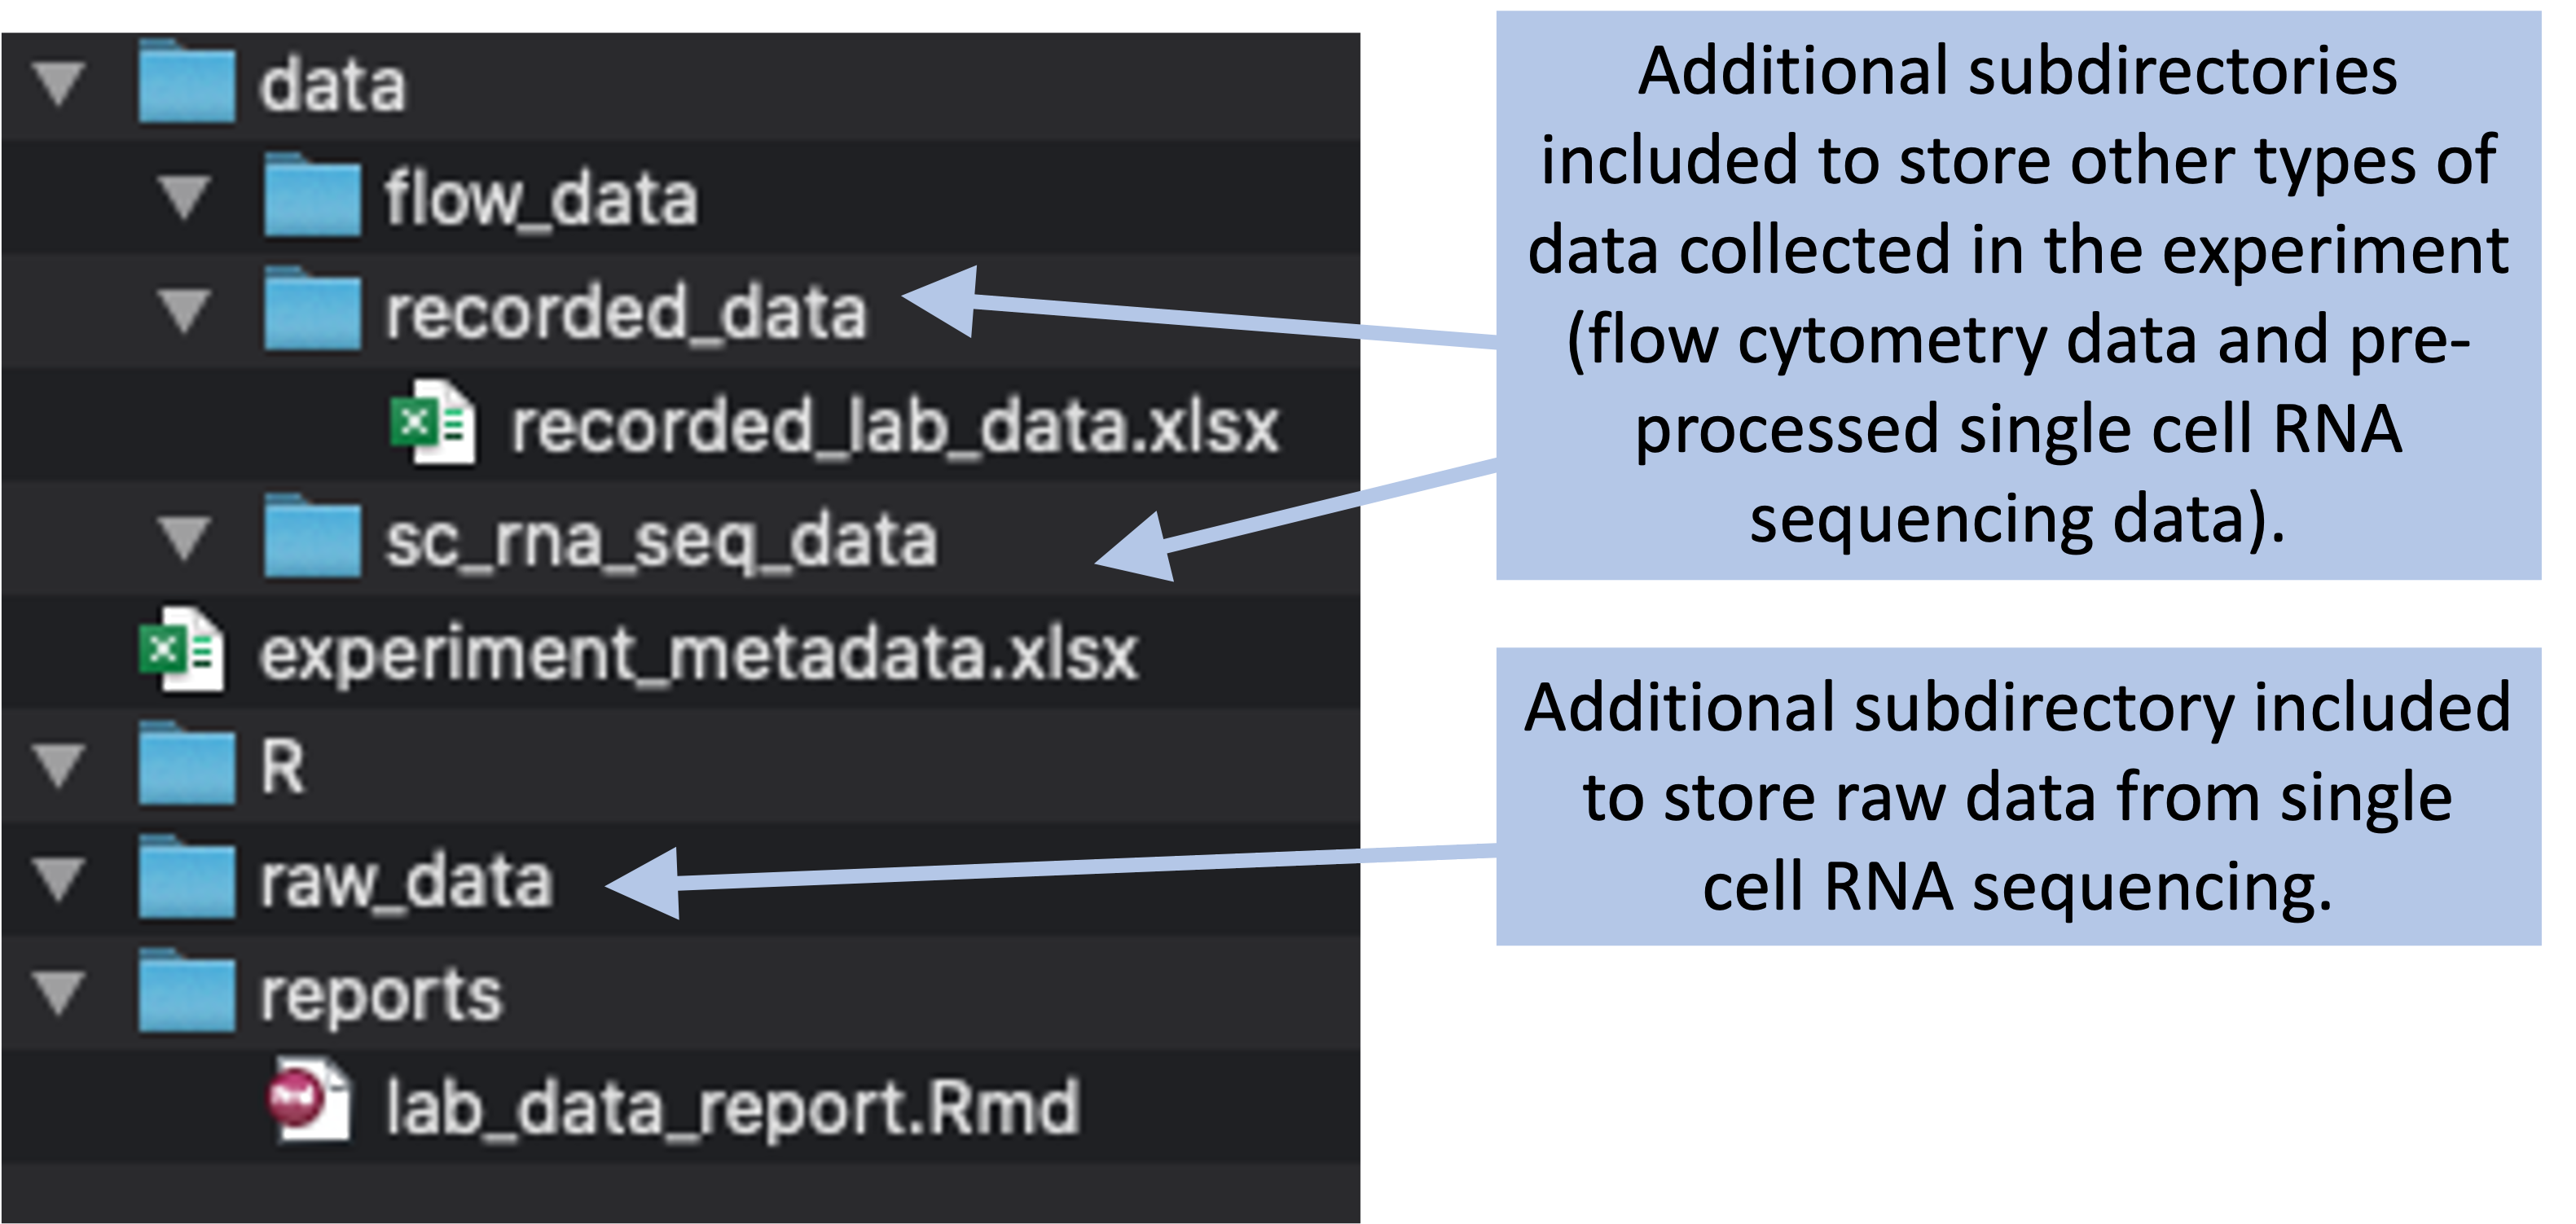
\includegraphics[width=\textwidth]{figures/project_template_morecomplex} \caption[Example of a more complex project directory structure that could be created, with directories added to store data collected through flow cytometry and single cell RNA sequencing]{Example of a more complex project directory structure that could be created, with directories added to store data collected through flow cytometry and single cell RNA sequencing.}\label{fig:projecttemplatecomplexmod8}
\end{figure}

Again, these subdirectories are named in a way that will generalize to many
different experiments and yet also clearly labels the contents. Similar
subdirectory diversions could also be used within the ``raw\_data'' subdirectory,
which would include files for data that need to be pre-processed before
they're used in statistical analysis (modules 3.1--3.3). For example, the
raw flow cytometry data will need to be gated---a process that will quantify
immune cell phenotypes in each sample---before it's used in statistical
analysis.

The exact combination of subdirectories within the ``data'' subdirectory might
change from experiment to experiment. For example, some experiments might
include single-cell RNA sequencing assays, while some may not. When we use the
template, it will be easy to delete any ``data'' subdirectories for assays we are
not conducting, but by including them in the template, we can insure that we use
a consistent name for each subdirectory when we do include it. If you're
trying to be consistent, it's easier to start with everything you might need
and delete some elements to customize for a particular project rather than
starting with a minimal framework and adding.

\subsection{Step 3: Establishing file name conventions}\label{step-3-establishing-file-name-conventions}

Next, we decided on how we'd name files in the directory. First, there are some
files that will be included in every project. These include a file to record
metadata about the experiment, as well as a file to record mouse weights over
the course of the experiment and bacterial load at the end of the experiment.

For both of these files, we selected filenames that would balance
generalizability with discoverability (see module 2.7 for more on setting rules
for filenames based on these principles). The file with experimental data, for
example, is named ``experiment\_metadata.xlsx''. This name is generic enough that
it will work for each of the studies, but it is also clear enough that people
will have a good idea of what's in the file when they explore the project
directory. Similarly, the file for recording weights and bacterial load is named
``recorded\_lab\_data.xlsx'', which again balances considerations generalizability
with discoverability.

You may have noticed that both these names avoid any special characters,
including spaces. Instead, the filenames use underscores to help distinguish
different words in the filenames and make them easy to read.

These experiments may have read-outs from laboratory equipment. Examples include
data from assays like flow cytometry and single-cell RNA sequencing. In these
cases, we'll keep the filenames that are generated by the laboratory equipment,
so that we'll maintain those standard formats.

\subsection{Step 4: Designing data collection templates}\label{step-4-designing-data-collection-templates}

The next step is to create any necessary data collection templates. We'll create
a separate spreadsheet for each type of data, but we can group them into files
if we'd like (e.g., one spreadsheet file with several separate sheets). In our
example, we created two files to store this type of data, one for the metadata
that are recorded at the start of the experiment (overall experiment details and
the details of each tested treatment) and one for the data that are collected
over the course of the experiment (mouse weights and bacterial loads). Within
each file, we've used separate sheets to record the different types of data.
This allows us to keep similar types of data together in the same file, while
having a tidy collection format for each specific type of data (Figure
\ref{fig:projectdatacollection}).

\begin{figure*}
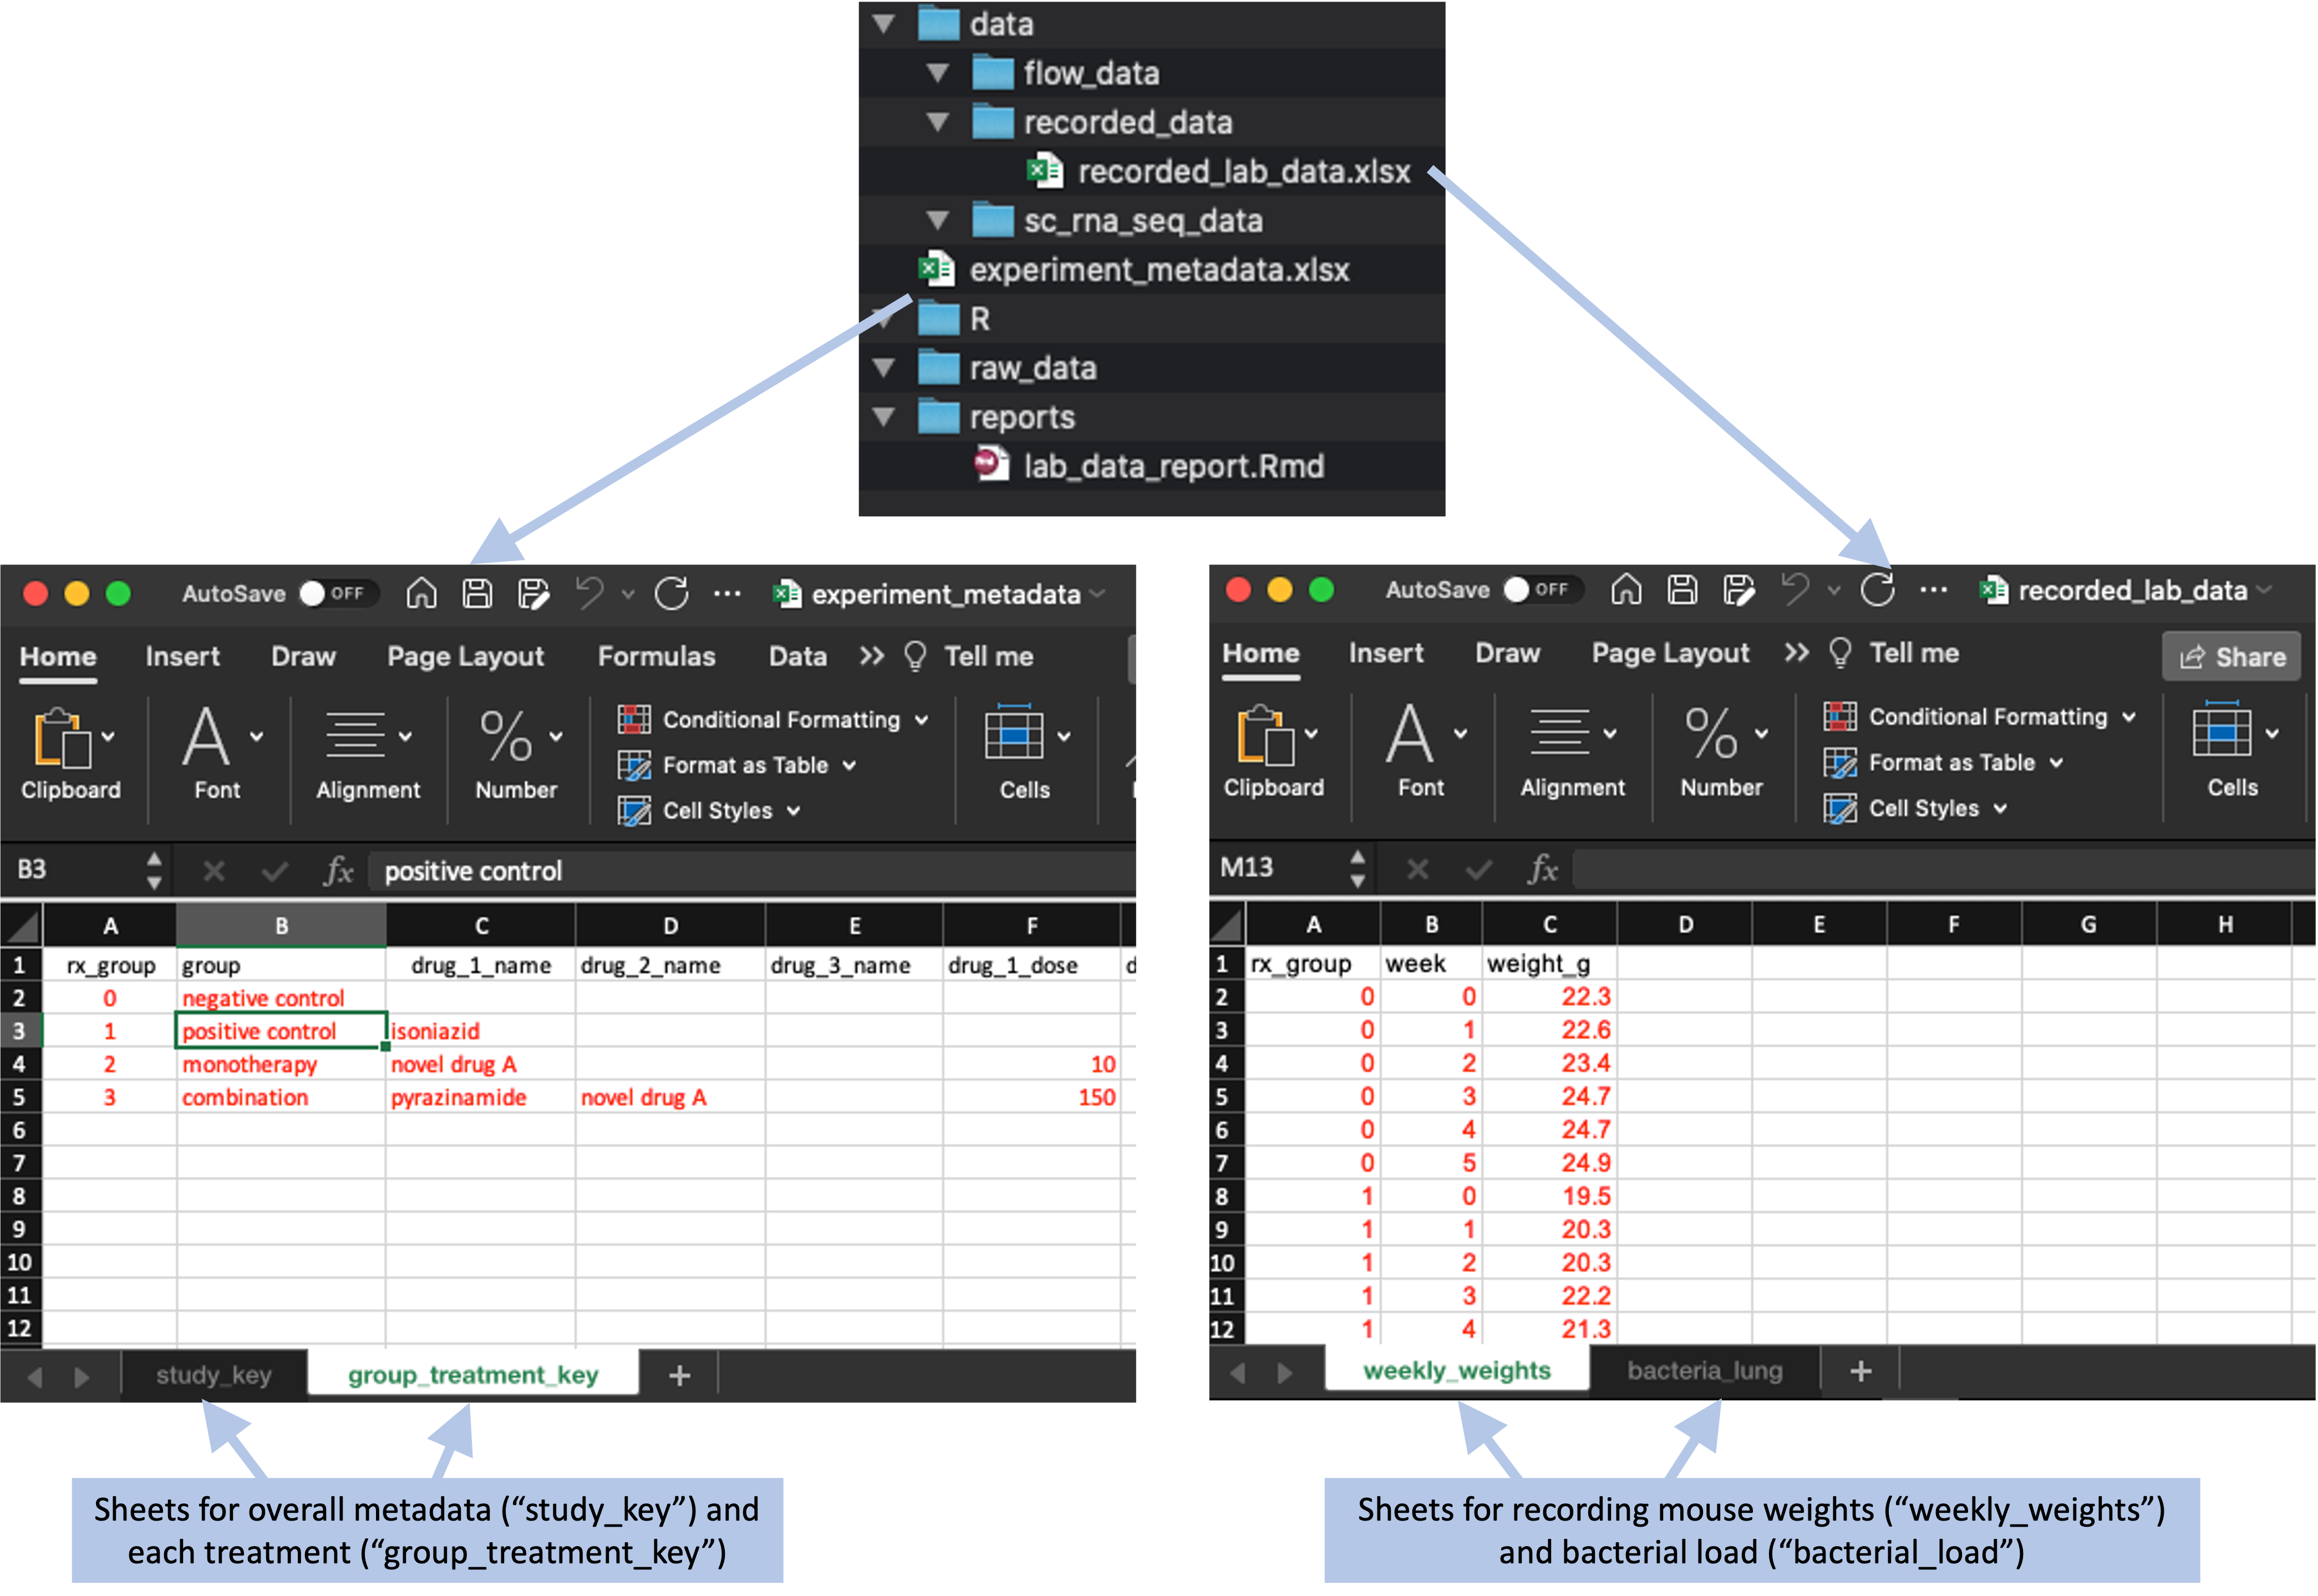
\includegraphics[width=\textwidth]{figures/project_data_collection} \caption[Data collection templates for the example project directory template]{Data collection templates for the example project directory template. These templates were created in two files, one for metadata, which is saved in the main directory of the project, and one for data collected in the laboratory during the experiment, which is saved in the 'data' subdirectory. Each file is saved as a spreadsheet file, with two sheets in each file to store different types of data.}\label{fig:projectdatacollection}
\end{figure*}

All of these data collection files are designed using the principles of tidy
data collection. In modules 2.4 and 2.5, we showed how you can create tidy data
collection templates to use, and how these can be paired with
reproducible reporting tools to separate the steps of data collection and
reporting (modules 3.7 through 3.9 go into much more depth on these reproducible
reporting tools). Once you have decided on the types of data that you will
usually collect for the type of study that this template is for, you can use
that process to create tidy data collection templates for each type of data.

When we created the template for each type of data, we added placeholder data
(formatted in red to indicate that it is placeholder, rather than final
data). This is so the researcher can see an example of how to enter data in
the template when they start a new project.

Figure \ref{fig:replacingplaceholdermetadata} gives an example of this process.
One of the files that is included in the example template directory shown
earlier is a spreadsheet to record metadata on the experiment. This spreadsheet
file has two sheets, one that records overall metadata on the study (for
example, the weeks of treatment given and the strain of mouse used) and one that
records details on each of the treatments that was tested. In the file in the
template directory, these spreadsheet pages include placeholder data. These are
formatted in red, so that they visually can be identified as placeholders. By
including these placeholder data, the researcher can see an example of the
format that you expect to be used in recording data in this file. Once the
project template is copied, the researcher will replace these data with the real
data, and then change the font color to black to indicate that the placeholder
data have been replaced (Figure \ref{fig:replacingplaceholdermetadata}).

\begin{figure*}
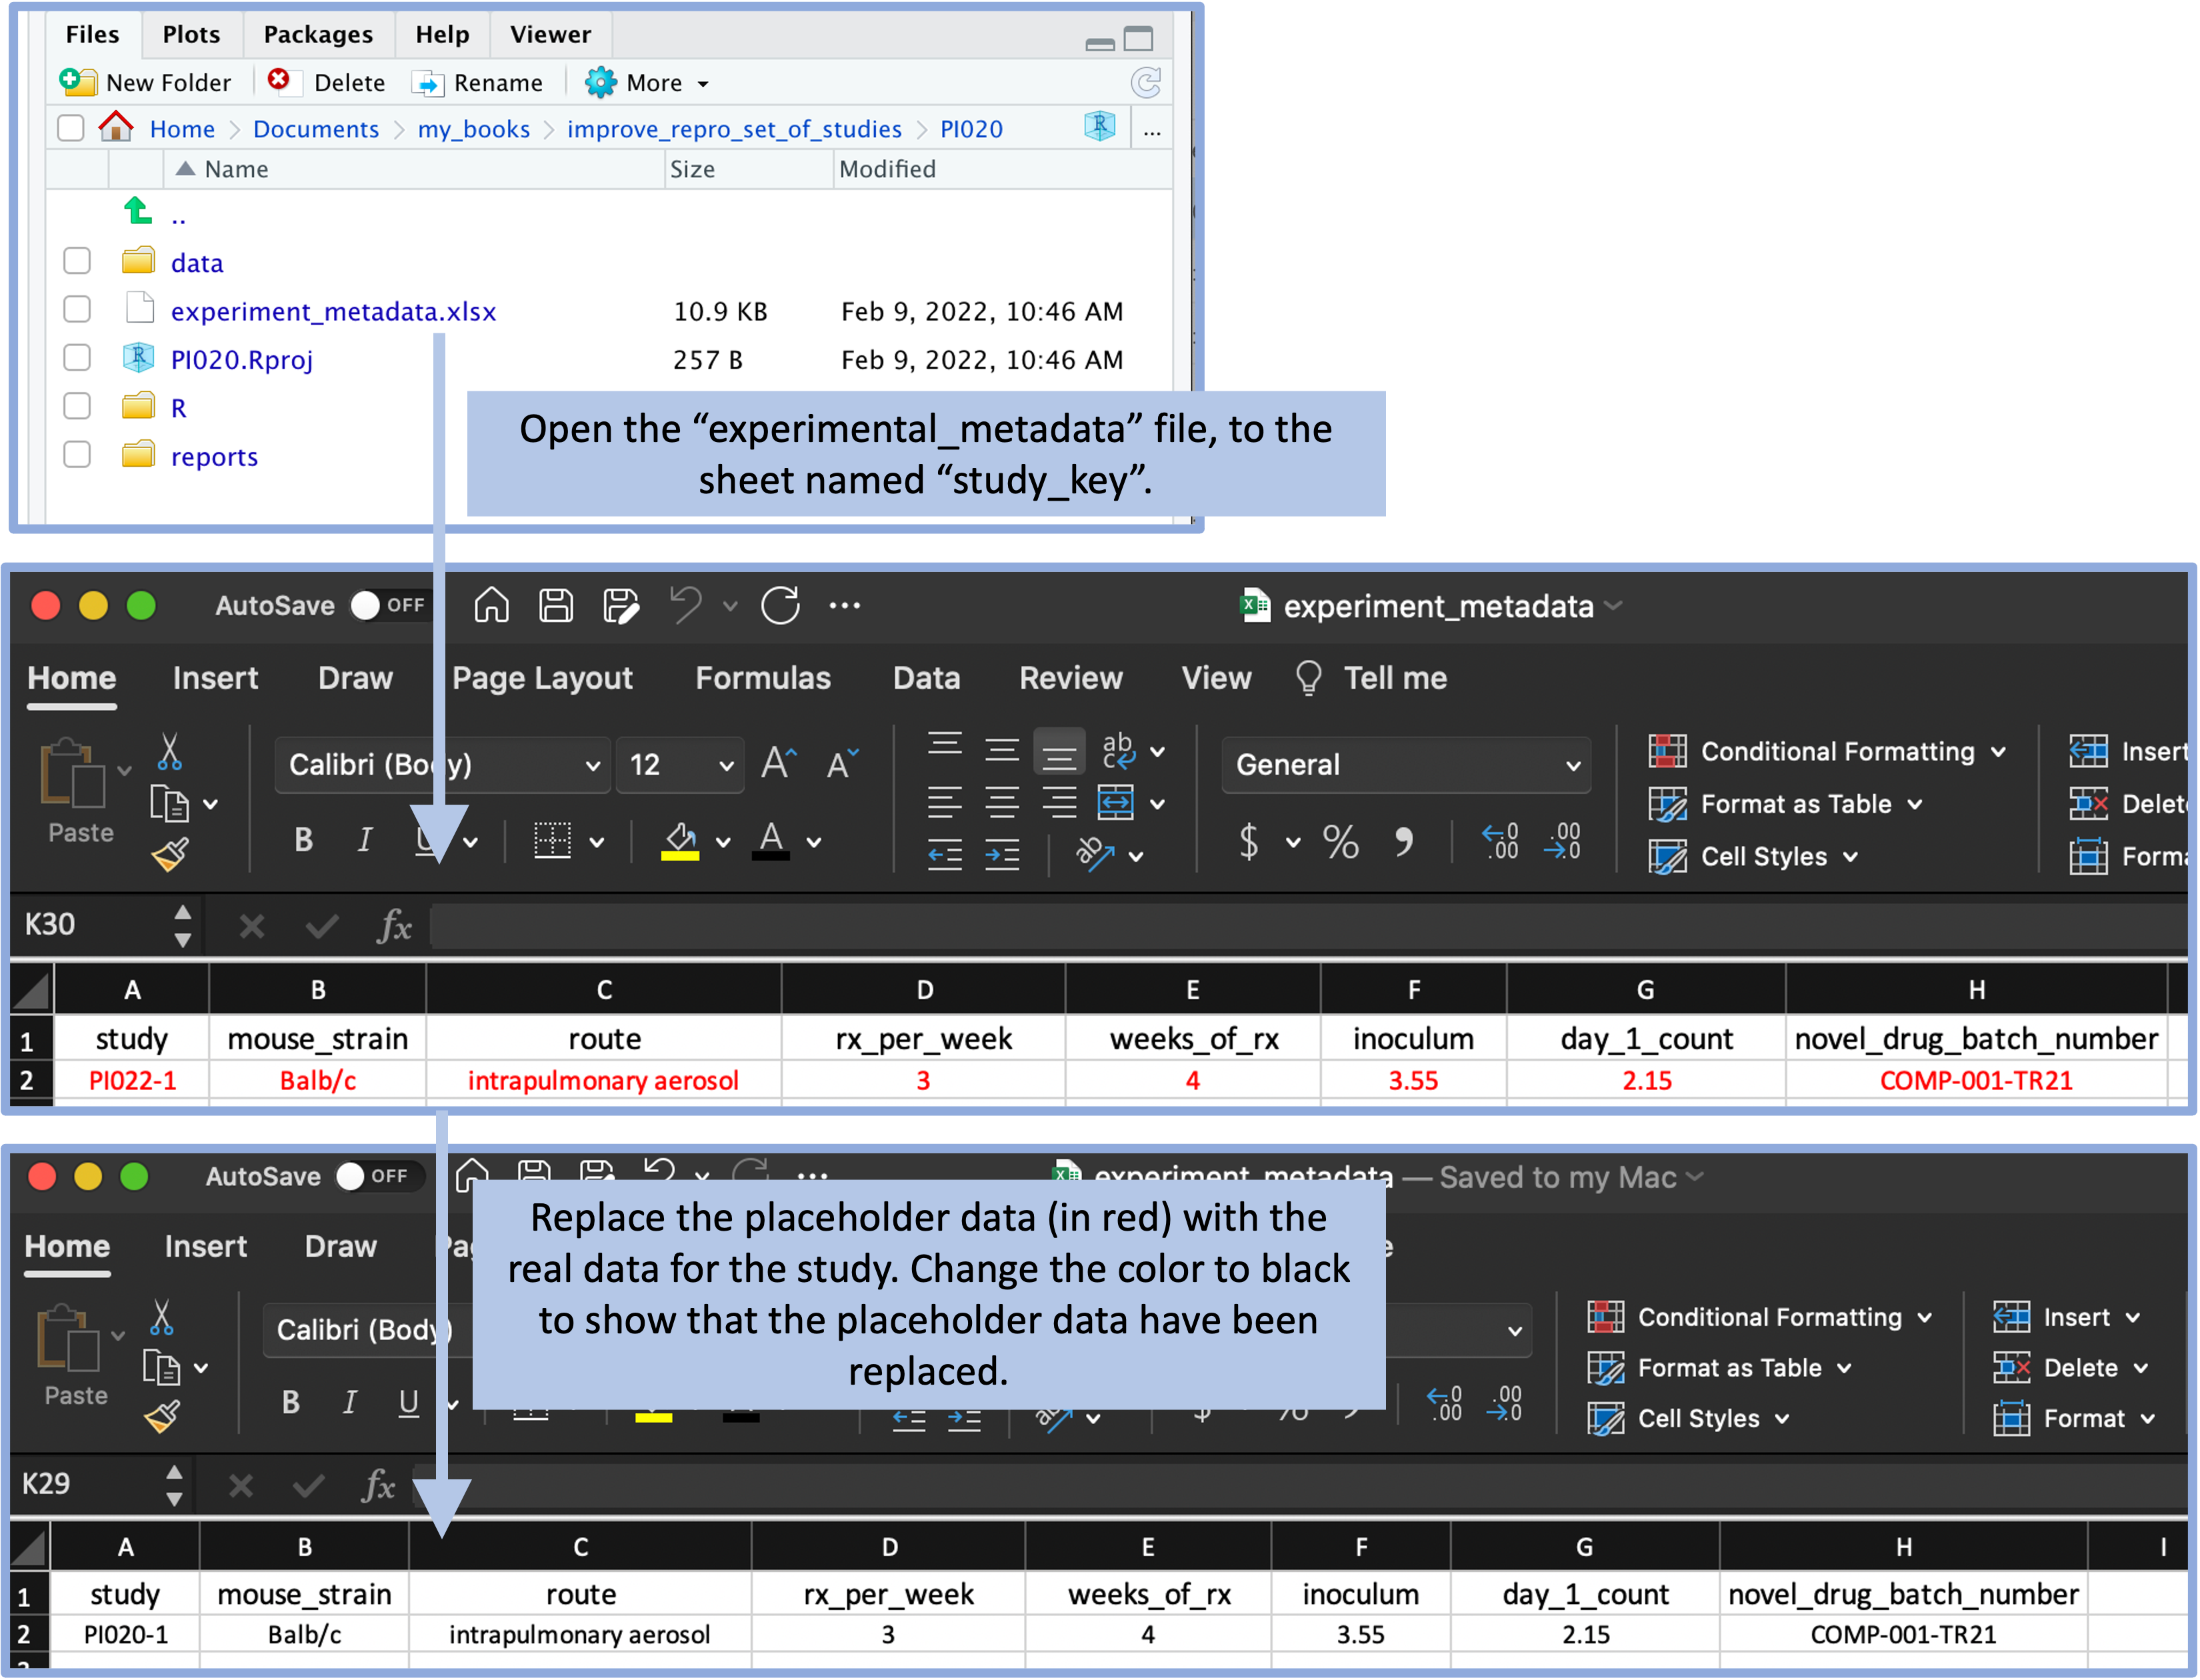
\includegraphics[width=\textwidth]{figures/project_replace_placeholder_metadata} \caption[The template includes a file with experiment metadata, with a sheet for recording the overall details of the experiment]{The template includes a file with experiment metadata, with a sheet for recording the overall details of the experiment. A user can open this file and replace the placeholder values (in red) with real values for the experiment. By changing the text color to black, the user can have a visual confirmation that the placeholder data have been replaced with real study data.}\label{fig:replacingplaceholdermetadata}
\end{figure*}

Another sheet of this spreadsheet allows the researcher to record the details of
each of the treatments that were tested in the experiment. Again, placeholder
data are included in the template in a red font to help show the researcher how
to record the data, and these are meant to be replaced with real data from the
specific experiment (Figure \ref{fig:replacingplaceholdertreatment2}). A
similar format is used in the template file to record data from the experiment,
including the weights of each animal over each week of treatment and the final
bacterial load in each animal at the end of treatment. Again, there are
placeholder values in the template file, which the researcher will replace with
real data after copying the project template for a new experiment.

\begin{figure*}
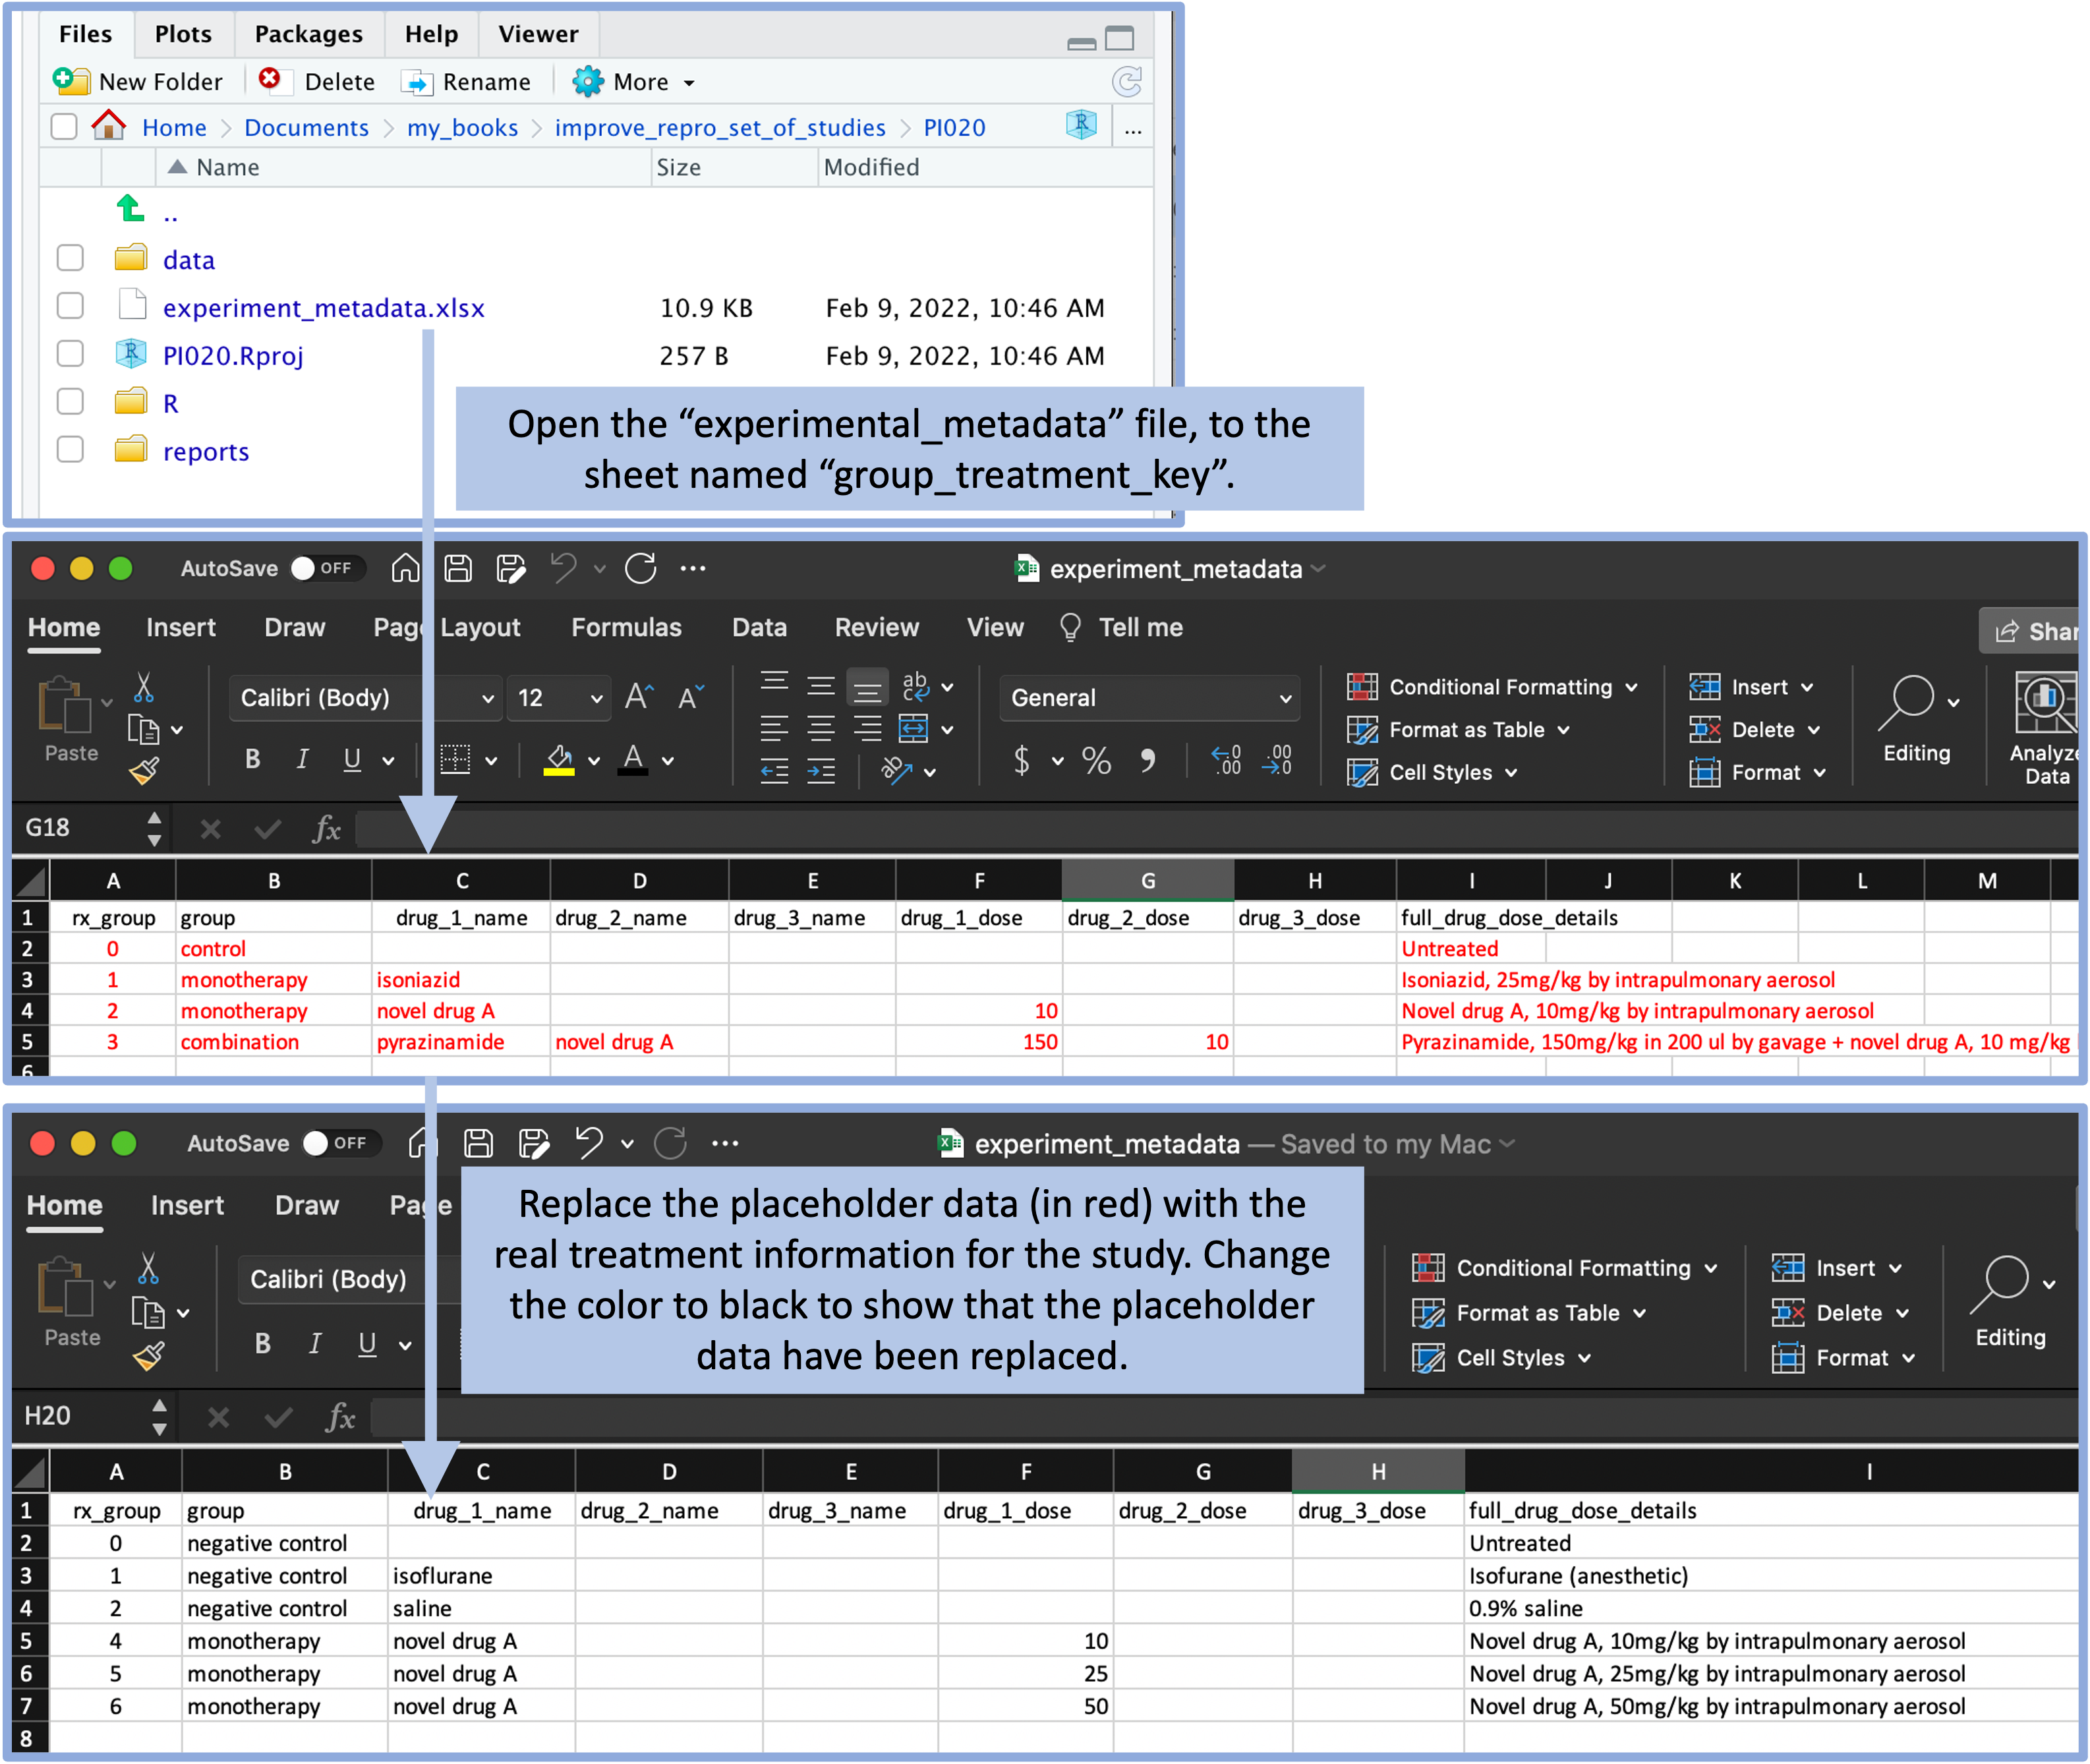
\includegraphics[width=\textwidth]{figures/project_replacing_placeholder_treatment_data} \caption[The template includes a file with experiment metadata, with a sheet for recording the details of each treatment]{The template includes a file with experiment metadata, with a sheet for recording the details of each treatment. A user can open this file and replace the placeholder values (in red) with real values for the treatments in the experiment. By changing the text color to black, the user can have a visual confirmation that the placeholder data have been replaced with real study data.}\label{fig:replacingplaceholdertreatment2}
\end{figure*}

\subsection{Step 5: Designing a report template}\label{step-5-designing-a-report-template}

A final and optional step is to create one or more template reports. You can
create report templates using tools for reproducible reports---in R, a key tool
for this is RMarkdown. Here, we'll cover using this tool for creating a report
briefly, but there are many more details in modules 3.7 through 3.9. Having
example files will help you to develop a template project report that can input
the type of data that you typically collect for this type of project.

We created an Rmarkdown file that does this analysis and visualization and
included it in the project template directory. This means that the report file
will be copied and available each time someone copies the project template
directory at the start of a new project. However, you are not obligated to keep
the report identical to the template. Instead, the template report serves as a
starting point, and you can add to it or adapt it as you work on a study.

This file is created using the RMarkdown format,
which combines text with executable code. You can create this template so that it
inputs the experimental data from the file formats created for the data recording
files in the project template. By doing this, the researcher should be able to ``knit''
this report for a new experiment, and it should recreate the report based on the
data recorded for that experiment (Figure \ref{fig:makingareport}). By knitting
this template report, you can create a nicely formatted version of the report for
the experimental data (Figure \ref{fig:examplereport1}).

\begin{figure*}
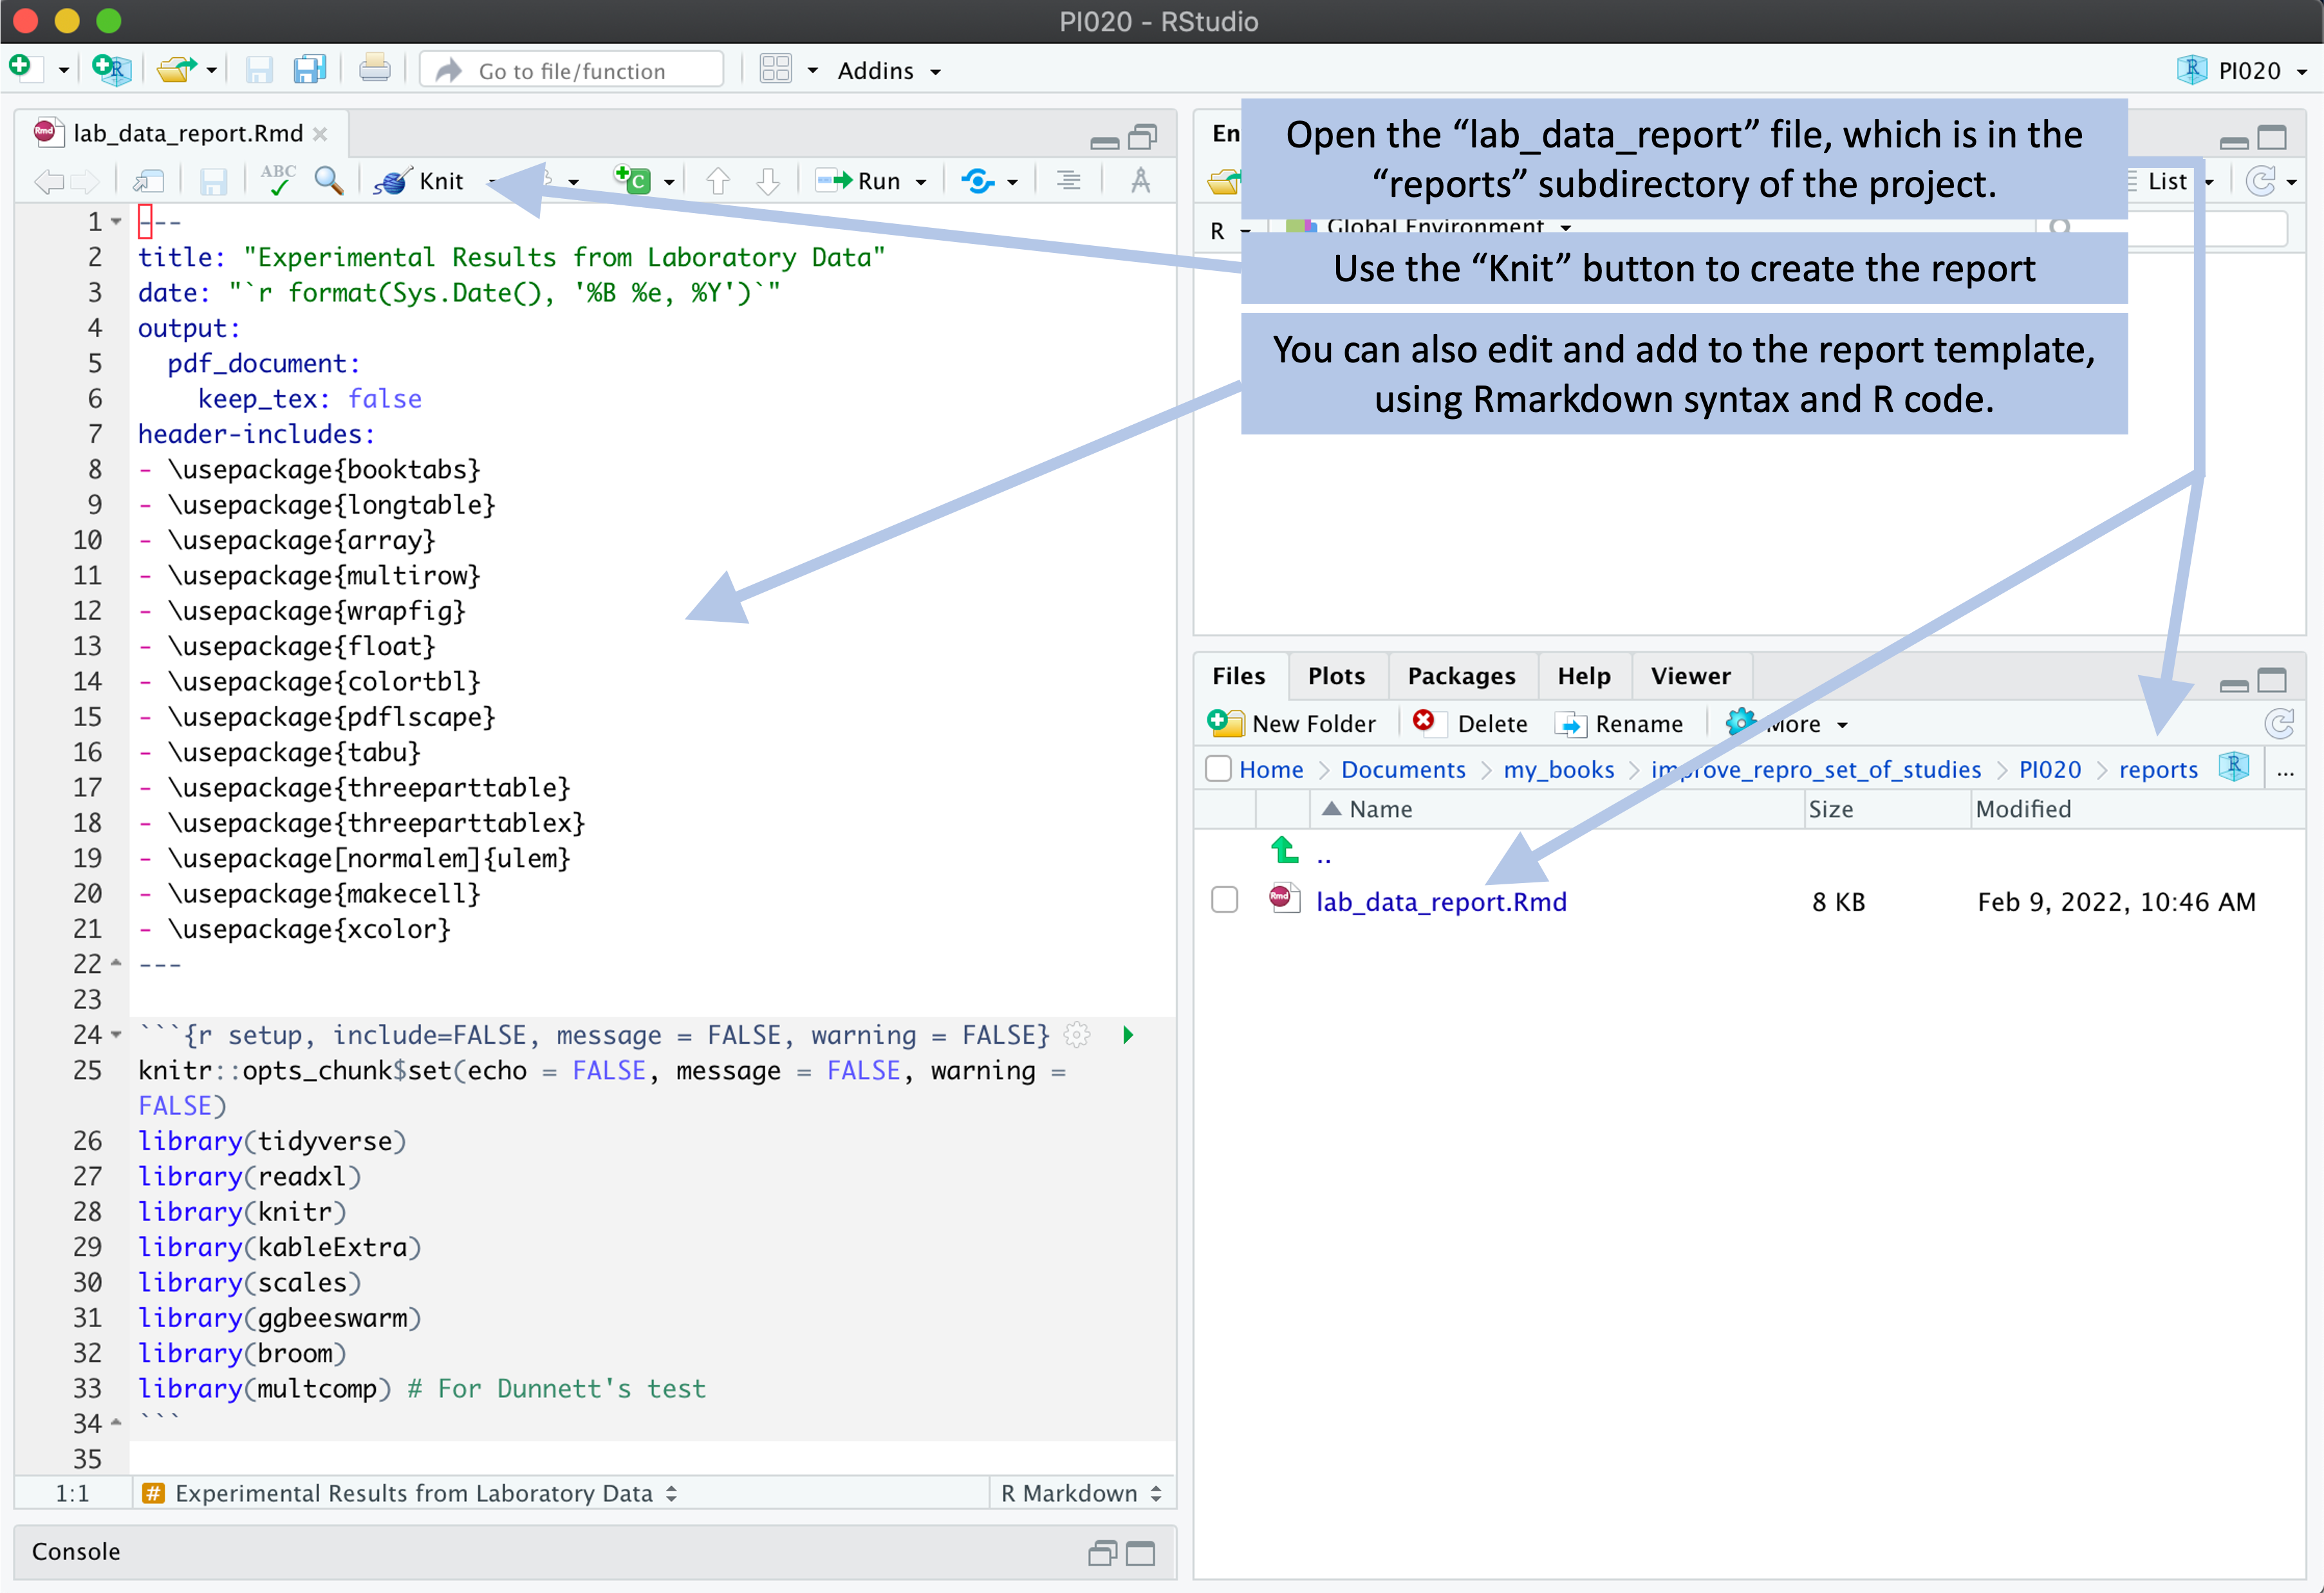
\includegraphics[width=\textwidth]{figures/project_opening_and_running_report} \caption[Example of how a user can create a report from the template]{Example of how a user can create a report from the template. The template includes an example report, which is written using RMarkdown. The user can open this template report file and use the 'Knit' button in RStudio to render the file. As long as the experimental data are recorded using the data template files, the code for this report can process the data to generate a report from the data. The user can also make changes and additions to the template report.}\label{fig:makingareport}
\end{figure*}

\begin{figure*}
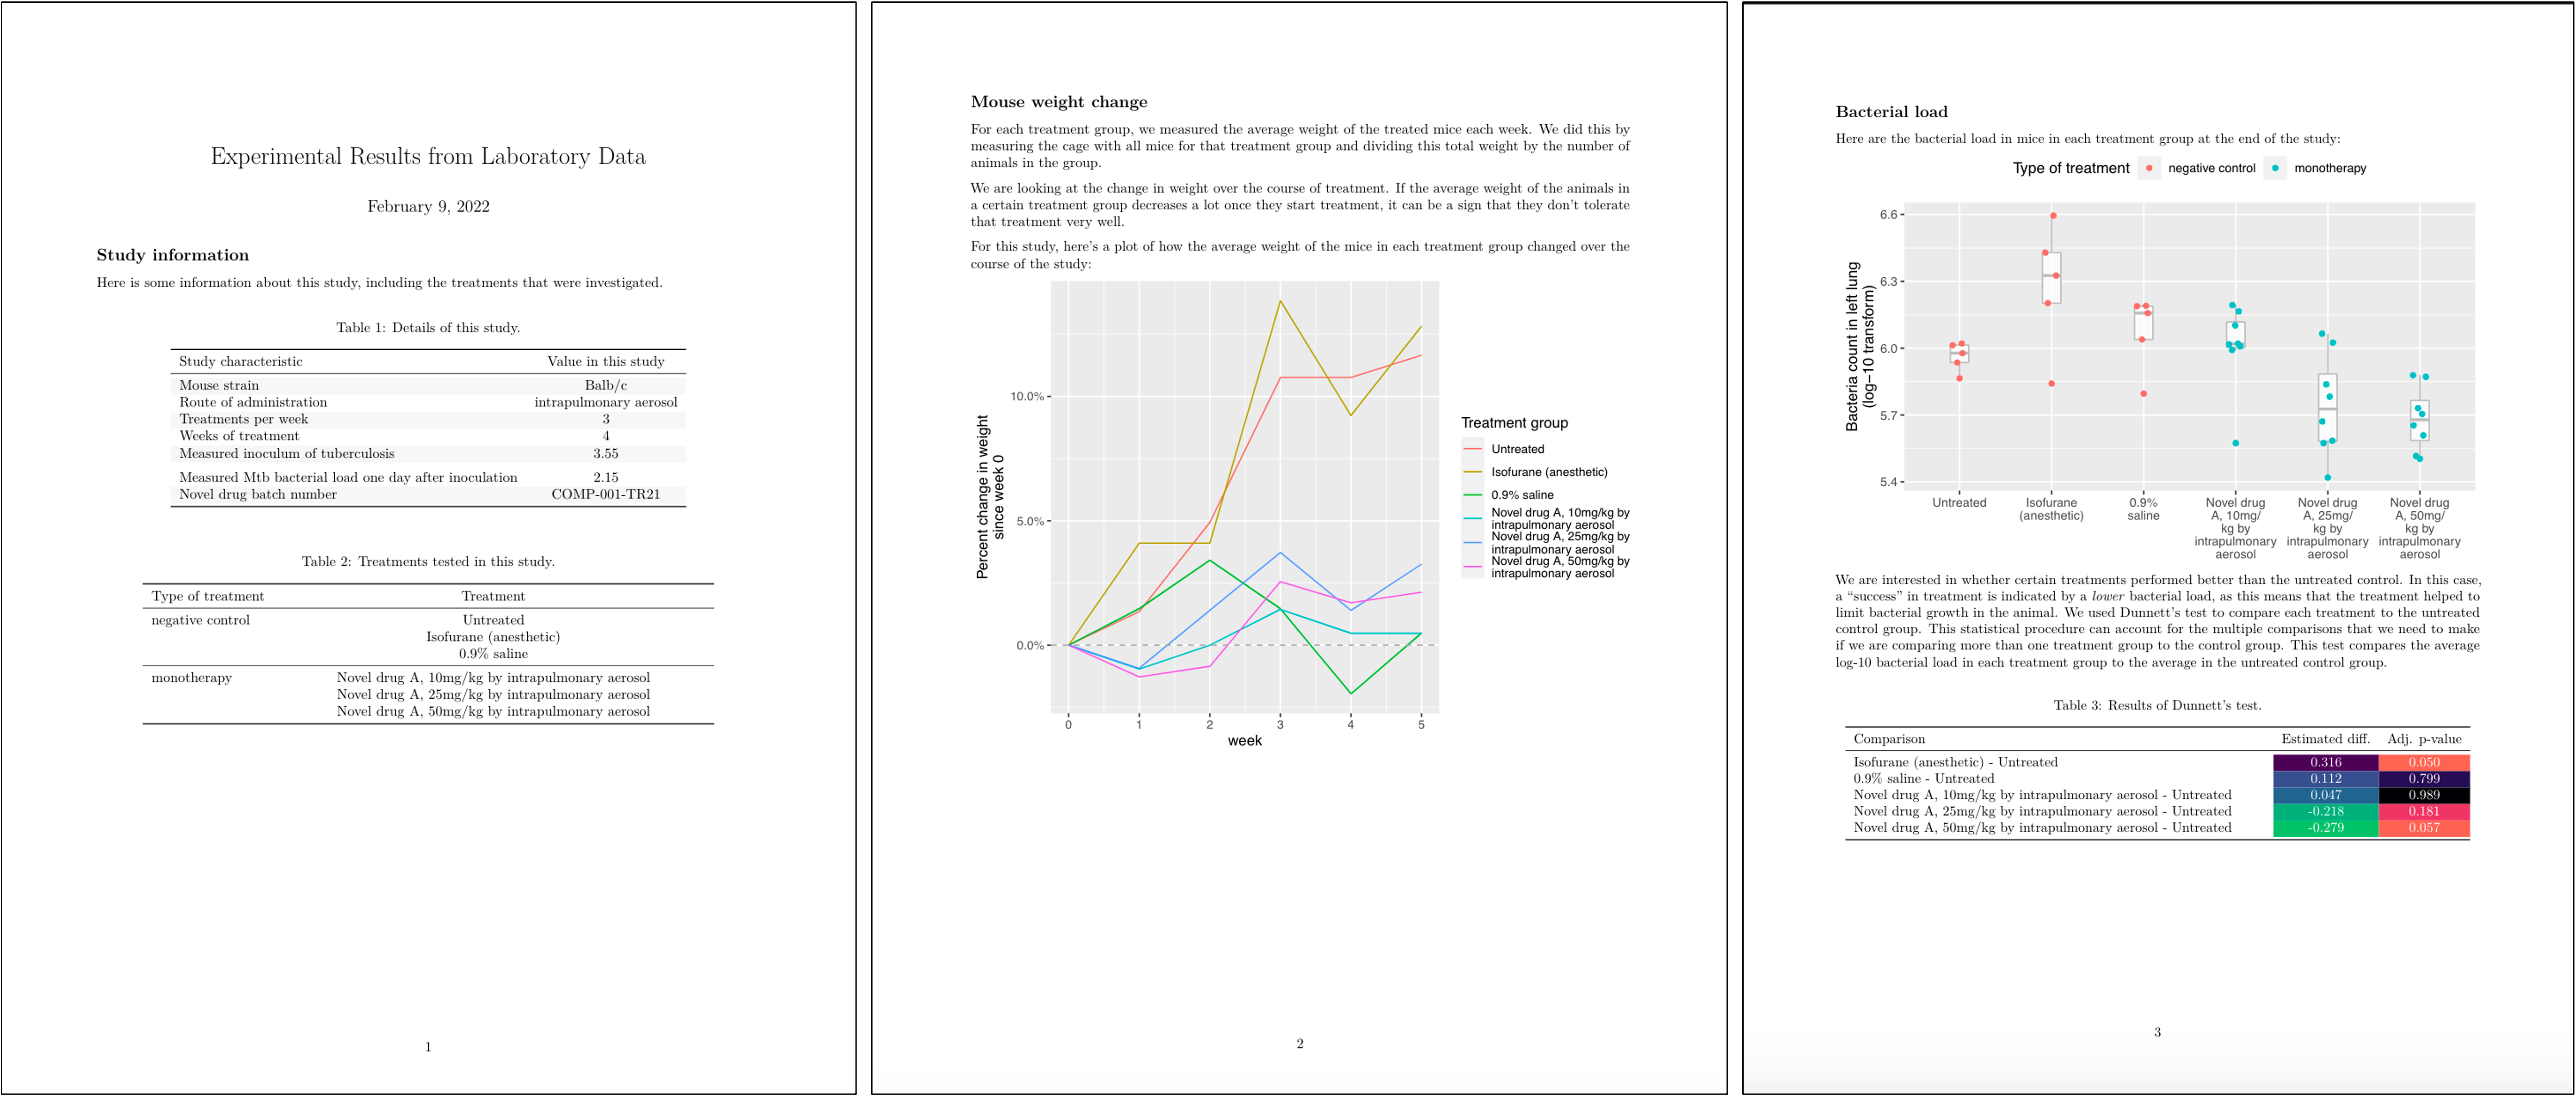
\includegraphics[width=\textwidth]{figures/project_example_report_study001} \caption[Example of the output from 'knitting' a report from the project template]{Example of the output from 'knitting' a report from the project template}\label{fig:examplereport1}
\end{figure*}

Specifically, for this set of studies a preliminary report was designed, with an
example shown in Figure \ref{fig:prelimreport}. This report uses the first page
to provide a nicely format version of the metadata for the study, including a
table with overall details and a table with details for each specific treatment
that was tested. The second page provides a graph that shows the percent weight
change for mice in each treatment group compared to the weight of that group at
the start of treatment. The third page provides a graph that shows the bacterial
loads in each mouse, grouped by treatment, as well as the results of running a
statistical test, for each treatment group, of the hypothesis that the mean
of a transformed version of the measure of bacterial load (log-10) for the group
was the same as for the untreated control group.

\begin{figure*}
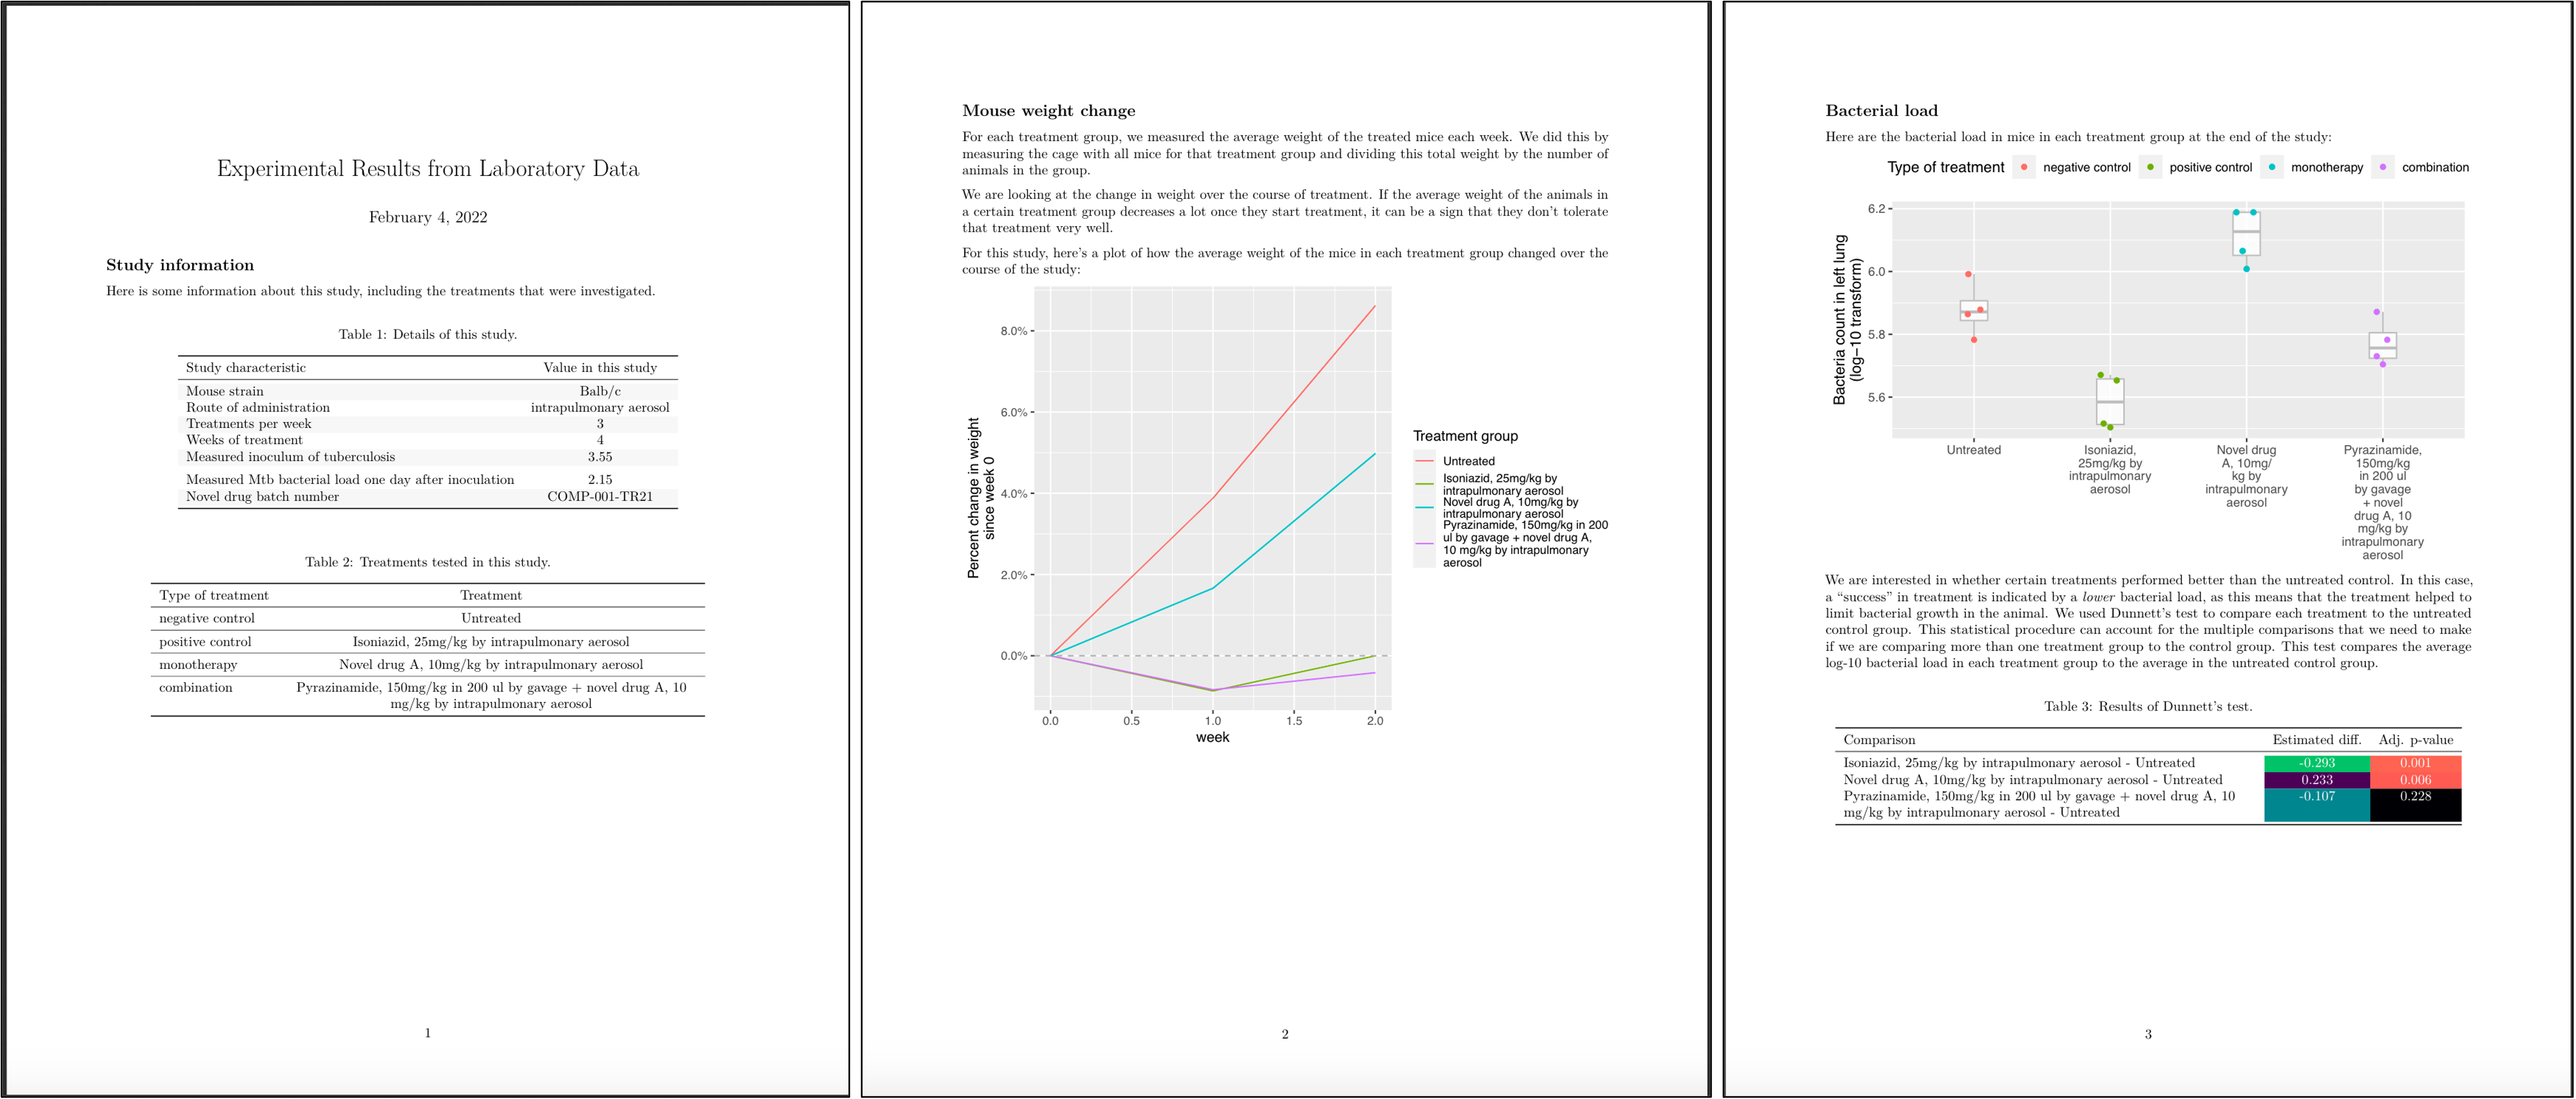
\includegraphics[width=\textwidth]{figures/project_prelim_report} \caption[Example of the preliminary report generated for each study in the set of example studies for this module]{Example of the preliminary report generated for each study in the set of example studies for this module. The first page includes metadata on the study, as well as details on each treatment that was tested. The second page shows how mouse weights in each treatment group changed over the course of treatment, to help identify if a treatment was well-tolerated. The third page graphs the bacterial load in each mouse, grouped by treatment, and gives the result of a statistical analysis to test which treatment groups had outcomes that were significantly different from the untreated control group.}\label{fig:prelimreport}
\end{figure*}

Let's take a closer look at a few of these elements. For example, Figure
\ref{fig:studytable} shows the tables from the first page of the report shown
in Figure \ref{fig:prelimreport}. If you look back to the data collection for
this study (e.g., Figures \ref{fig:metadata} and \ref{fig:treatmentdetails}),
you can see that all of the information in these tables was pulled from data
recorded at the start of the study.

\begin{figure*}
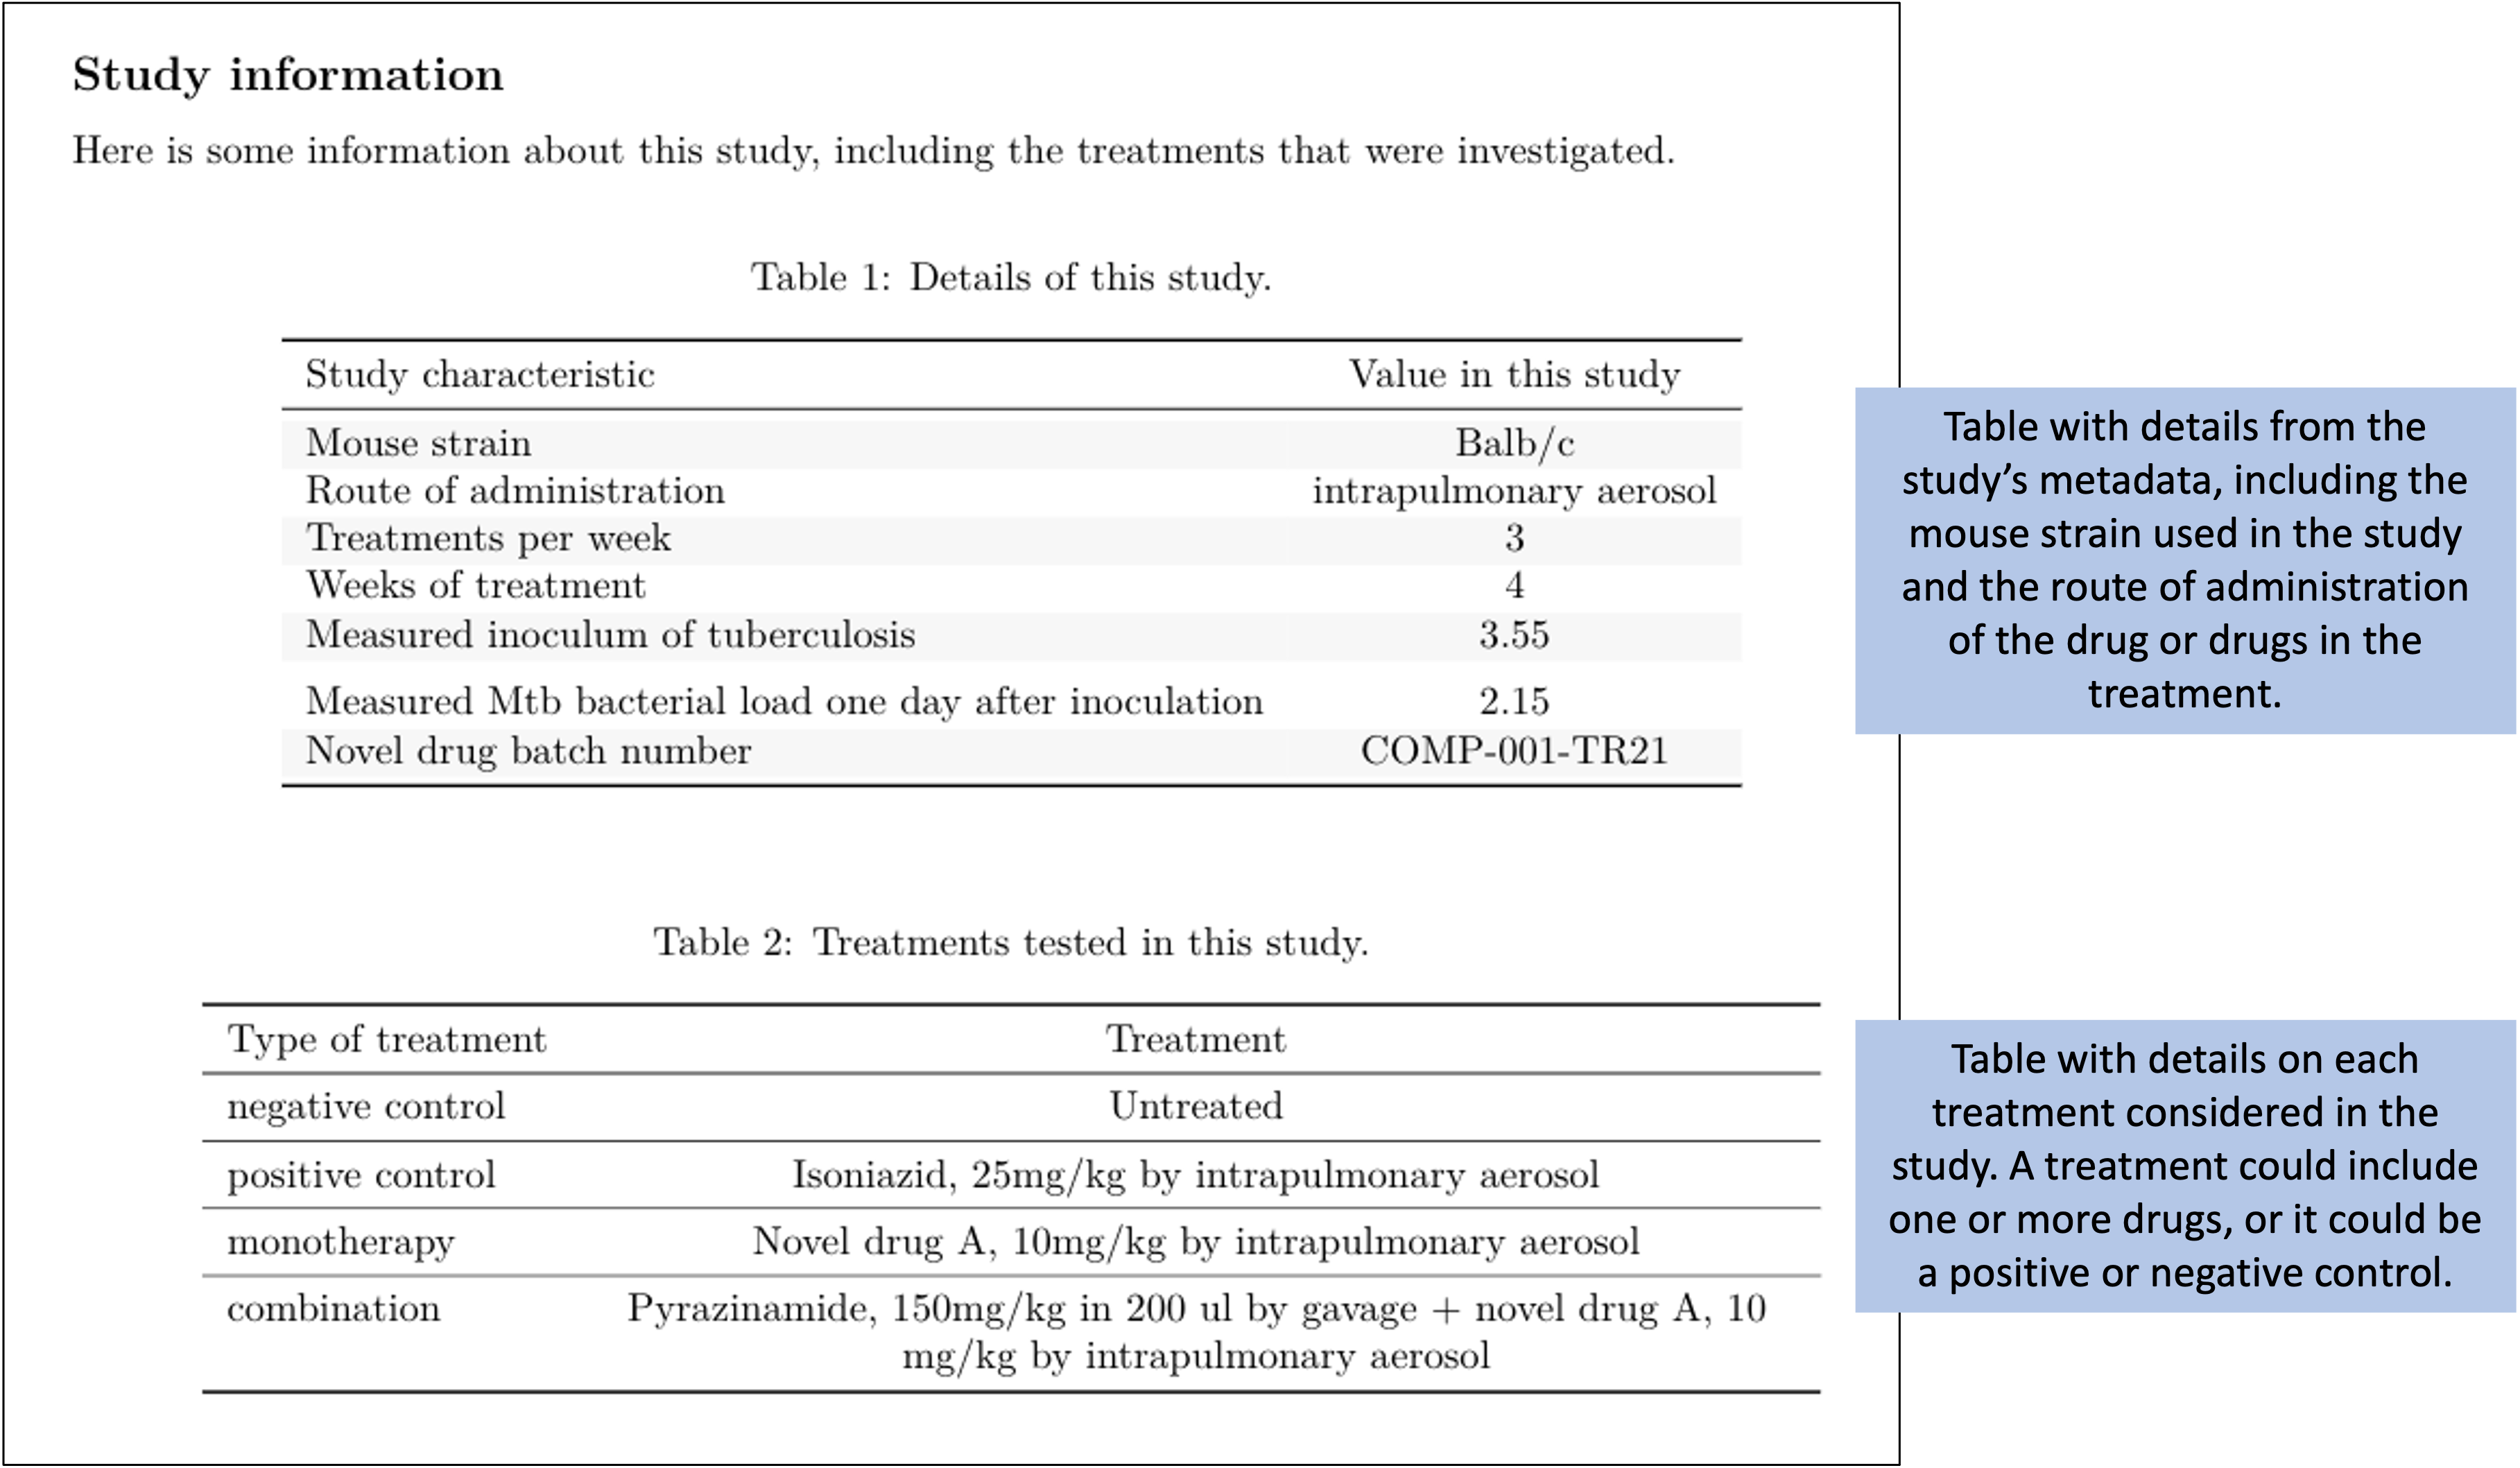
\includegraphics[width=\textwidth]{figures/project_study_info_table} \caption[Example of one element of the preliminary report generated for each study in the set of example studies for this module]{Example of one element of the preliminary report generated for each study in the set of example studies for this module. The first page provides tables with metadata about the study and details about each treatment that was tested.}\label{fig:studytable}
\end{figure*}

Figure \ref{fig:mouseweightsplot} shows the second page of the report. This
figure has taken the mouse weights---which were recorded in one of the data
collection templates for the project (Figure \ref{fig:mouseweight})---and used
them to generate a plot of how average mouse weight in each treatment group
changed over the course of the treatment.

\begin{figure*}
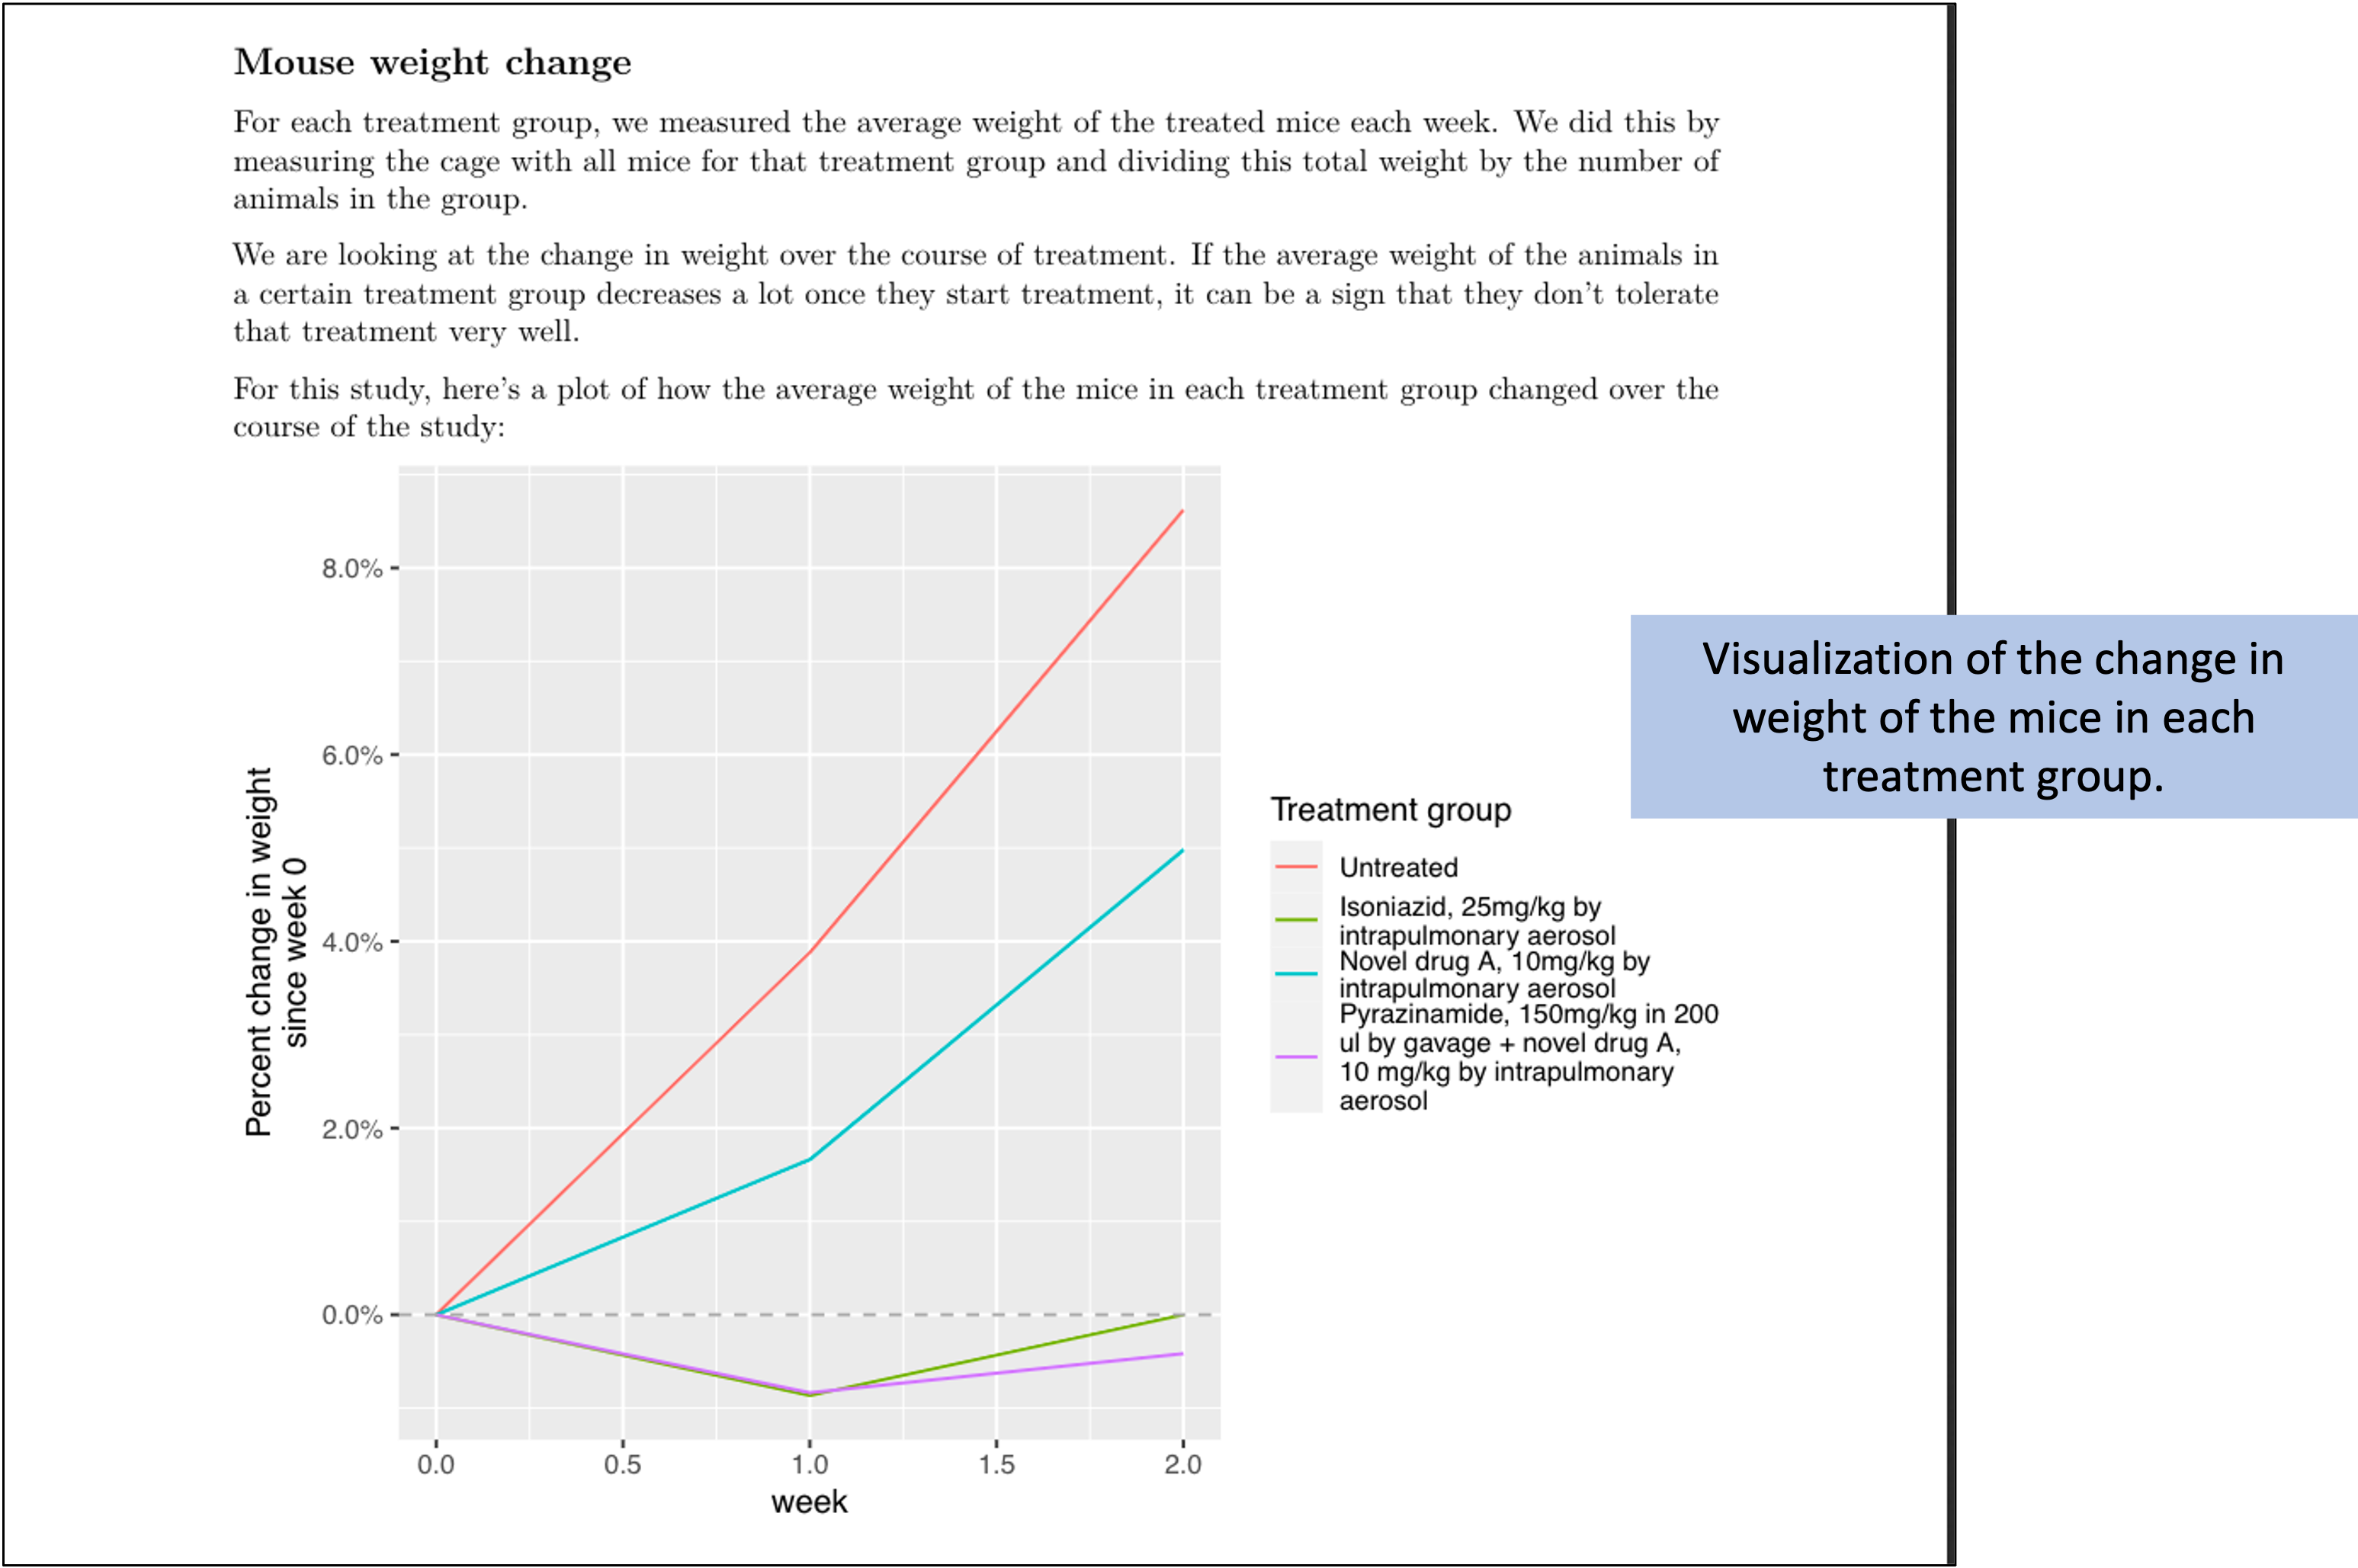
\includegraphics[width=\textwidth]{figures/project_mouse_weights_graph} \caption[Example of one element of the preliminary report generated for each study in the set of example studies for this module]{Example of one element of the preliminary report generated for each study in the set of example studies for this module. The second page provides a plot of how the weights of mice in each treatment changed over the course of treatment.}\label{fig:mouseweightsplot}
\end{figure*}

Figure \ref{fig:bactcompare} shows the last page of the report. This page
starts with a figure that shows the bacterial load in the lungs of each mouse in
the study at the end of the treatment period. In this figure, the measurement
for each mouse is shown with a point, and these points are grouped by the
treatment group of the mouse. Boxplots are added to show the distribution across
the mice in each group. The color is used to show whether the treatment was a
negative control, a positive control, a monotherapy, or a combined therapy. The
second part of the page gives a table with the results from running a
statistical analysis to compare the bacterial load for mice in each treatment
group to the bacterial load in the mice in the untreated control group. Color is
added to the table to highlight treatments that had a large difference in
bacterial load from the untreated control, as well as treatments for which the
difference from the untreated control was estimated to be statistically
significant. All the data for these results, including the labels for the plot,
are from the data collected in the data collection templates shown earlier.

\begin{figure*}
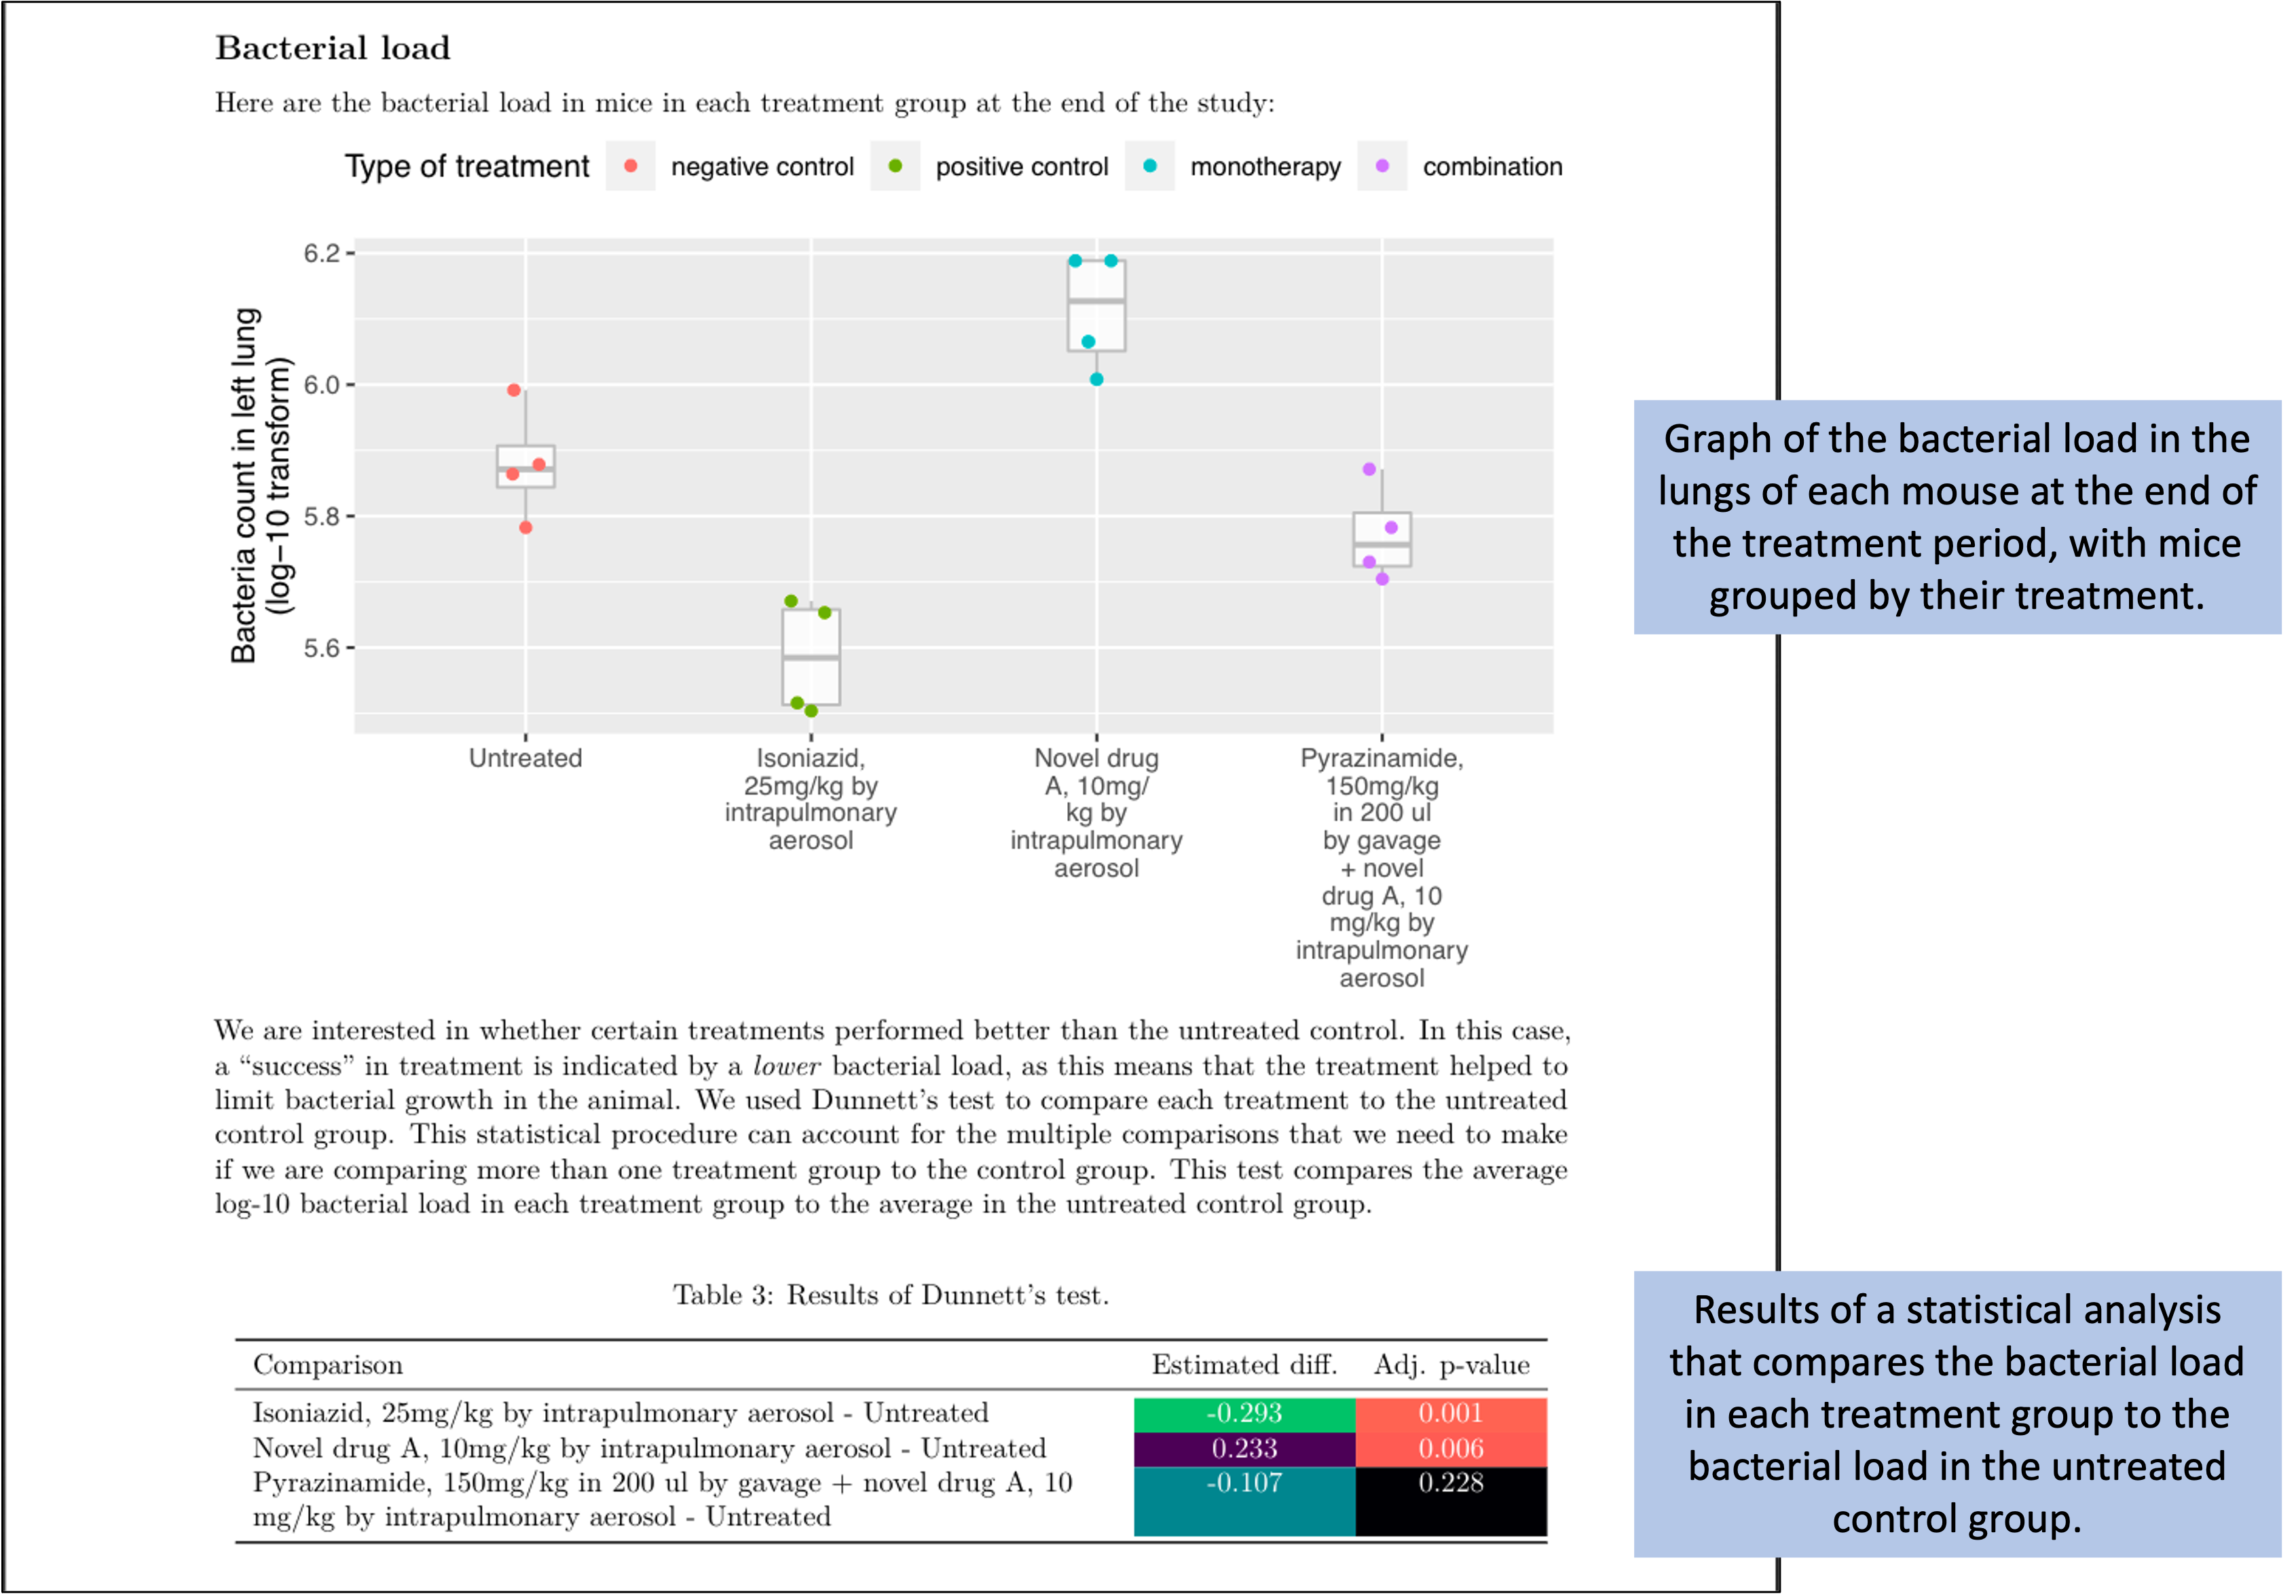
\includegraphics[width=\textwidth]{figures/project_bact_compare_plot} \caption[Example of one element of the preliminary report generated for each study in the set of example studies for this module]{Example of one element of the preliminary report generated for each study in the set of example studies for this module. The third page provides results on how bacterial load in the lungs compares among treatments at the end of the treatment period.}\label{fig:bactcompare}
\end{figure*}

We wrote the code in the report in a way that it will still run if there are
more or fewer observations in any of the data collection files, so the report
template has some flexibility in terms of how each study in the set of studies
might vary. For example, in the example set of studies, some of the experiments
were run using only a control group of mice, while others were run to test
several different treatment groups. The report template can accommodate
these differences across studies in the set of studies.

\section{Harnessing version control for transparent data recording}\label{module9}

As a research project progresses, researchers will often end up with many files
(e.g., `draft1.doc', `draft2.doc'). This can result in an explosion of files,
and it becomes hard to track which files represent the ``current'' state of a
project. Version control allows researchers to edit and change research project
files more cleanly, while including messages to explain changes and maintaining
the power to backtrack to previous versions.

In this module, we will explain what version control is and how it can be used
in research projects to improve the transparency and reproducibility of
research, particularly for data recording. We'll introduce you
to the basic idea of version control, using the Git software program as an
example. In later modules, we'll explain version control platforms like GitHub,
as well as give some tips on how to use both within your research projects.

\textbf{Objectives.} After this module, the trainee will be able to:

\begin{itemize}
\tightlist
\item
  Define ``version'', ``version control'', ``version control software'',
  ``repository'', ``commit'', and ``commit message''
\item
  Discuss challenges in coordinating changes in project files when working
  in teams
\item
  List some downsides of physical laboratory notebooks
\item
  Distinguish between ``version control'' and ``version control software''
\item
  Identify examples of versioning in a digital context (data, code, files)
\item
  Discuss how version control principles can improve collaboration in
  scientific projects
\end{itemize}

\subsection{Challenges of collaborating on evolving research materials}\label{challenges-of-collaborating-on-evolving-research-materials}

When research groups---or any other professional teams---collaborate on
publications and research, the process can be a bit haphazard. Teams often use
emails and email attachments to share updates on the project, and they sometimes
use email attachments to pass around the latest version of a document for others
to review and edit.

One fascinating example comes from the business world. After the implosion of
Enron, a trove of emails from within the company were released. This set of
emails has become known as the Enron Corpus and has been used for a variety of
research studies. One group of researchers investigated emails from this corpus
that involved people who were doing work with spreadsheets \citep{hermans2015enron}.
They found that passing Excel files through email attachments was a common
practice, and that messages within emails suggested that spreadsheets were
stored locally, rather than in a location that was accessible to all team
members \citep{hermans2015enron}. This meant that team members might often be
working on different versions of the same spreadsheet file. They note that ``the
practice of emailing spreadsheets is known to result in serious problems in
terms of accountability and errors, as people do not have access to the latest
version of a spreadsheet, but need to be updated of changes via email.''
\citep{hermans2015enron} The same process for collaboration is often used in
scientific research: one study found, ``Team members regularly pass data files
back and forth by hand, by email, and by using shared lab or project servers,
websites, and databases.'' \citep{edwards2011science}

These practices make it very difficult to keep track of all project files, and
in particular, to track which version of each file is the most current. Further,
this process constrains patterns of collaboration---it requires each team member
to take turns in editing each file, or for one team member to attempt to merge
in changes that were made by separate team members at the same time when all
versions are collected.

This process also makes it difficult to keep track of why changes were made, and
often requires one team member to approve the changes of other team members.
While ``Track changes'' and ``Comment'' features in software like Microsoft Word can
help the team communicate with each other, these features often lead to a very
messy document at stages in the editing, where it is hard to pick out the
current versus suggested wording, and once a change is accepted or a comment
deleted, these conversations can be lost forever. Finally, word processing tools
are poorly suited to track changes or add suggestions directly to data or code,
as both data and code are usually saved in formats that aren't native to word
processing programs, and copying them into a format like Word can introduce
problematic hidden formatting that can cause the data or code to malfunction.

\subsection{Recording data in the laboratory---from paper to computers}\label{recording-data-in-the-laboratoryfrom-paper-to-computers}

More and more scientific researchers are tackling these challenges in their own
projects using something called \emph{version control}. But how does version
control---traditionally a tool of software engineers---relate to collaborating
to collect and analyze scientific research data? Traditionally, experimental
data collected in a laboratory was recorded in a paper laboratory notebook.
These laboratory notebooks played a role not only as the initial recording of
data, but also keep a legal record of the data recorded in the lab
\citep{mascarelli2014research}. They were also a resource for collaborating across a
team and for passing on a research project from one lab member to another
\citep{butler2005electronic}.

However, paper laboratory notebooks have a number of limitations. First, they
can be very inefficient. In a time when almost all data analyses---even simple
calculations---are done on a computer, recording research data on paper rather
than directly entering it into a computer is inefficient. Also, any stage of
copying data from one format to another, especially when done by a human rather
than a machine, introduces the chance to copying errors. Handwritten laboratory
notebooks can be hard to read \citep{butler2005electronic, perkel2011coding}, and
they may lack adequate flexibility to handle the complex experiments often
conducted. Further, electronic alternatives can also be easier to search,
allowing for deeper and more comprehensive investigations of the data collected
across multiple experiments \citep{giles2012digital, butler2005electronic, perkel2011coding}. As one article notes, physical lab notebooks are ``usually
chaotic and always unsearchable'' \citep{perkel2011coding}.

Given a widespread recognition of the limitations of paper laboratory notebooks,
in the past couple of decades, there have been a number of efforts, both formal
and informal, to move from paper laboratory notebooks to electronic
alternatives. In some fields that rely heavily on computational analysis, there
are very few research labs (if any) that use paper laboratory notebooks
\citep{butler2005electronic}. In other fields, where researchers have traditionally
used paper lab notebooks, companies have been working for a while to develop
electronic laboratory notebooks specifically tailored to scientific research
\citep{giles2012digital}. Some early adapters were pharmaceutical industrial
labs, where companies had the budgets to get customized versions and the
authority to require their use. In academic laboratories, electronic lab
notebooks have taken longer to be adapted \citep{giles2012digital, butler2005electronic}. Indeed, a widely adopted platform for electronic laboratory
notebooks has yet to be taken up by the scientific community \citep{kwok2018lab},
despite clear advantages of recording data directly into a computer rather than
first using a paper notebook. As Kwok notes in a 2018 commentary,

\begin{quote}
``Since at least the 1990s, articles on technology have predicted the imminent,
widespread adoption of electronic laboratory notebooks (ELNs) by researchers. It has
yet to happen'' \citep{kwok2018lab}
\end{quote}

Instead of using customized electronic laboratory notebook software, some
academics are moving their data recording online, but are using more generalized
electronic alternatives, like Dropbox, Google applications, OneNote, and
Evernote \citep{perkel2011coding, kwok2018lab, giles2012digital, powell2012lab}.
Some scientists have started using version control software, especially the
combination of Git and GitHub, as a way to improve laboratory data recording,
and in particular to improve transparency and reproducibility standards.
These pieces of software share the same pattern as Google applications or
Dropbox---they are generalized tools that have been honed and optimized for ease
of use through their role outside of scientific research, but can be harnessed
as a powerful tool in a scientific laboratory, as well. They are also free---at
least, for GitHub, at the entry and academic levels---and, even better, one
(Git) is open-source.

\subsection{Defining ``version'' and ``version control''}\label{defining-version-and-version-control}

Most scientific research today involves collaboration across a team of
researchers, rather than an individual scientist working alone. Collaboration
drives interdisciplinary science, but it also creates challenges. One
challenge comes with coordinating versions of research materials. These
materials can include data collection files, but can also include other
documents like study protocols, as well as physical materials like cell lines,
antibodies, and model organisms.

A \emph{version} is one iteration of a research material that is evolving. For
example, a draft of a research paper is one version of that paper. Research data
that you collect may also go through several versions. For example, if you
identify a typo in data after you record it, you may need to correct the typo
and add a note or signature to explain that update. Further, if you are
collecting data at multiple timepoints, you may have new versions of a data file
as you complete each timepoint.

As materials evolve across versions, it introduces challenges in maintaining a
research process that is smooth, efficient, and error-free. One challenge is to
make sure it is always clear which version is the most current, as well as which
version should be used for specific purposes. For example, if several coauthors
are editing a paper draft, it is important to ensure they are all working on the
most recent version.

Another challenge is to coordinate the changes that different people make when
they work on the material at the same time. Scientific collaboration often does
not operate as an assembly line, where one person finishes their work on a
document or material and then hands it off to the next person. Instead, there
will often be several copies of a version in different peoples' hands, with all
of them working on it at once. One example is a paper draft---often coauthors
all edit the latest draft at the same time, rather than one-by-one.
This creates the challenge of taking the contributions of each person and
coordinating their changes and additions into one primary copy.

A third challenge is to keep track of the changes that are made at each step, as
the document moves from version to version. This record can help in auditing for
errors or bugs that might be introduced as the document evolves. Ideally, the
record also will include some information about why changes were made at each
step.

These challenges can be addressed through a process called \emph{version control}.
While the term is most commonly used in reference to software development, the
idea of version control is widely relevant. Any process that creates evolving
versions of a document or material can benefit from the idea of version control,
which aims to record and document changes to the material over time, coordinate
the contributions of different members of a team, and revert back to older
versions if needed. In this module, we'll focus on version control as it applies
to research materials that are electronic (files and directories), but you may
also find it useful to think about how the principles and elements of version
control can be applied to other research materials, like cell lines and
antibodies.

\subsection{What are the key elements of version control?}\label{what-are-the-key-elements-of-version-control}

The term \emph{version} in \emph{version control} refers to one iteration or state of a
document or set of documents, for example the current version of a data file.
The word \emph{control} captures the idea of allowing for safe changes and updates to
the version, especially when more than one person is working on it. Part of this
``control'' will also include recording the changes made from one version to the
next and annotating reasons for those changes.

The general term \emph{version control} can refer to any method of syncing
contributions from several people to a file or set of files. Version control of
computer files can be done ``by hand'', with a person manually logging each change,
and originally was \citep{irving2011astonishments}. However, it's much more efficient
to use a computer program to handle this tracking and to coordinate
contributions from multiple people. As Eric Raymond notes in \emph{The Art of Unix
Programming}, ``tracking all that detail is just the sort of thing computers are
good at and humans are not'' \citep{raymond2003art}. He goes on to describe version
control as ``a suite of programs that automates away most of the drudgery
involved in keeping an annotated history of your project and avoiding
modification conflicts'' \citep{raymond2003art}.

Software for this purpose---\emph{version control software}---was first developed for
software programming projects. Some popular version control software today
comes from these roots. In this section, we'll introduce the key features of
version control, and to do so we'll use examples and terminology from a common
version control software program called Git. While these terms are derived
from this particular software program, they represent ideas that are important
in any implementation of version control. Later, we'll touch on how some of these
ideas are incorporated in other software, like Google Docs.

The software available for version control tracks electronic files. While the
very earliest version control software systems tracked single files, these
systems quickly moved to tracking sets of files, called \emph{repositories}. A
repository is almost identical to a file directory (which you may also know as a
file folder), and indeed a repository starts from a file directory. The only
difference is the repository is enhanced with some additional overhead
\citep{klemens201421st}. This overhead is added to record how the files in the
directory have changed over time. You can compare this to how you might track
document changes if the documents were paper rather than electronic---you could
store the documents in a paper folder and add a piece of paper where you record
a log of each change you make to the documents in the folder. The extra overhead
that changes a regular file directory to a repository is very similar to the log
in this example. A repository, in other words, is a directory that is under
version control.

In a repository of files that is under version control, the version control
software takes snapshots of how the files look during your work on them. Each
snapshot is called a \emph{commit}, and it provides a record of which lines in each
file changed from one snapshot to another, as well as exactly how they changed.
The idea behind these commits---recording the differences, line-by-line, between
an older and newer version of each file derives from a longstanding Unix command
line tool called \emph{diff}. This tool, developed early in the history of Unix at
AT\&T's Bell Labs \citep{raymond2003art}, is a solid and well-tested tool that does
the simple but important job of generating a list of all the differences between
two plain text files. Each commit in a repository includes the same type of
information about the differences introduced in the files at the time of that
commit.

When you are working with a directory under version control, you explain your
changes as you make them---in other words, version control allows for annotation
of the developing and editing process \citep{raymondunderstanding}. Each commit
requires you to enter a \emph{commit message} describing why the changes in that
commit were made. The commit messages can serve as a powerful tool for
explaining changes to other team members or for reminding yourself in the future
about why certain changes were made. A repository under version control, then,
can include not only a complete history of how files in a project directory have
changed over the course of the project, but also why. If this feature is used
thoughtfully, then the commit history of the project provides a well-documented
description of the project's full evolution. If you're working on a manuscript,
for example, when it's time to edit, you can cut whole paragraphs, and if you
ever need to get them back, they'll be right there in the commit history for
your project, with their own commit message about why they were cut. If you make
the commit message clear, it will make it easy to find that commit if you ever
need those paragraphs again.

Further, each of the commits is given its own ID tag (in the Git software,
this is done through something called a unique SHA-1 hash \citep{klemens201421st}),
and version control systems have a number of commands that let you ``roll back''
to earlier versions. This provides \emph{reversability} within the project files,
allowing you to go back to the version as it was when a certain commit was made
\citep{raymondunderstanding}.

It turns out that this functionality---of being able to roll back to earlier
versions---has a wonderful side benefit when it comes to working on a large
project. It means that you don't need to save earlier versions of each file. You
can maintain one and only one version of each project file in the project's
directory, with the confidence that you never ``lose'' old versions of the file
\citep{perkel2018git, blischak2016quick}. This allows you to maintain a clean and
simple version of the project files, with only one copy of each, ensuring it's
always clear which version of a file is the ``current'' one (since there's only
one version) \citep{klemens201421st}. This also provides the reassurance that you can
try new directions in a project, and always roll back to the old version if that
direction doesn't work well.

In a 2011 commentary in \emph{Nature Methods}, Perkel tells a story about how this
functionality helped one researcher keep his project directories simpler:

\begin{quote}
``Early in his graduate career, John Blischak found himself creating figures
for his advisor's grant application. Blischak was using the programming language
R to generate the figures, and as he iterated and optimized his code, he ran
into a familiar problem: Determined not to lose his work, he gave each new
version a different filename---analysis\_1, analysis\_2, and so on, for
instance---but failed to document how they had evolved. `I had no idea what had
changed between them,' says Blischak\ldots{} Using Git, Blischak says, he no longer
needed to maintain multiple copies of his files. `I just keep overwriting it and
changing it and saving the snapshots. And if the professor comes back and says,
'oh, you sent me an email back in March with this figure', I can say, `okay,
well, I'll just bo back to the March version of my code and I can recreate
it'.'' \citep{perkel2018git}
\end{quote}

A key strength, then, of using version control is its ability to track every
change made to files in the project, why the change was made, and who made it.
Version control creates a full history of the evolution of each file in the
project. When a change is committed, the history records the exact change made,
including the previous version of the file. No change is ever fully lost,
therefore, unless a great deal of extra work is taken to erase something from
the project's commit history.

It's also helpful to understand how version control programs handle
collaboration. In earlier types of version control programs, under what is
called a \emph{centralized} framework, there was one central repository for the file
or set of files the team was working on \citep{raymondunderstanding, target2018version, irving2011astonishments}. A team member who wanted to make
a change would ``check out'' the file he or she wanted to work on, make changes,
and then check it back in as the newest main version \citep{raymond2003art}. While
one team member had this file checked out, other members would be locked out of
making any changes to that file---they could look at it, but couldn't make any
edits \citep{raymondunderstanding, target2018version}. This meant that there was no
chance of two people trying to change the same part of a file at the same time.
In spirit, this early system is pretty similar to the idea of sending a file
around the team by email, with the understanding that only one person works on
it at a time. A slightly more modern analogy is the idea of having a single
version of a file in Dropbox or Google Docs, and avoiding working on the file
when you see that another team member is working on it.

This assembly-line approach is pretty clunky, though. In particular, it usually
increases the amount of time that it takes the team to finish the project,
because only one person can work on a file at a time. Later types of version
control programs moved toward a different style, allowing for \emph{distributed}
rather than centralized collaborative work on a file or a set of files
\citep{raymondunderstanding, irving2011astonishments}. Under the distributed model,
all team members can have their own version of all the files, work on them and
make records of changes they make to the files, and then occassionally sync with
everyone else to share your changes with them and bring their changes into your
copy of the files. This functionality is called \emph{concurrency}, since it allows
team members to concurrently work on the same set of files
\citep{raymondunderstanding}.

This idea allowed for the development of other useful features and styles of
working, including \emph{branching} and \emph{forking}. Branching allows you to try out
new ideas that you're not sure you'll ultimately want to go with. Forking is a
key tool used in open-source software development, and, among other things,
facilitates someone who isn't part of the original team getting a copy of the
files they can work with and suggesting some changes that might be helpful. So,
this is the basic idea of modern version control---for a project that involves a
set of computer files, everyone on the team has their own copy of the directory
on their own computer, makes changes at the time and in the spots in the files
that they want, and then regularly re-syncs their local directory with everyone
else's to share changes and updates.

This distributed model also means there is a copy of the full repository on
every team member's computer, which has the side benefit of providing additional
backup of the project files. Remote repositories---which may be on a server in a
different location---can be added with another copy of the project, which can
similarly be synced regularly to update with any changes made to project files.

\subsection{Comparing Git to other tools}\label{comparing-git-to-other-tools}

While there are a number of software systems for version control, one of the
most common currently used for scientific projects is Git. This program was
created by Linus Torvalds, who also created the Linux operating system, in 2005
as a way to facilitate the team working on Linux development. This program for
version control thrives in large collaborative projects, for example open-source
software development projects that include numerous contributors, both regular
and occasional \citep{brown2018git}. As Target notes in a 2018 article about
version control:

\begin{quote}
``While people sometimes grouse about its steep learning curve or unintuitive
interface, Git has become everyone's go-to for version control.''
\citep{target2018version}
\end{quote}

In recent years, some complementary tools have been developed that make the
process of collaborating together using version control software easier. Other
tools, such as bug trackers or issue trackers, facilitate corroborative
file-based projects to allow the team to keep a running ``to-do'' list of what
needs to be done to complete the project. These tools---which are discussed in
modules 2.10 and 2.11---can be used to improve collaboration on scientific
projects done by teams. GitHub is one a very popular version control platform
with these additional tools. It was created in 2008 as a web-based platform to
facilitate collaborating on projects running under Git version control. It can
provide an easier entry to using Git for version control than trying to learn to
use Git from the command line \citep{perez2016ten}. It also interfaces well with RStudio,
making it easy to integrate a collaborative workflow through GitHub from the
same RStudio window on your computer where you are otherwise doing your analysis
\citep{perez2016ten}.

While Git version control software is one of the best established ways
of implementing version control, there are growing efforts to enable some level
of version control through other platforms. For example, Google Docs enables a
level of version control through its Version History feature. This feature
allows you name different versions of a document as they are is saved in Google
Docs. It also allows you to restore a document to earlier versions, as well as
see which changes have been made to a document and who made each change.

While some generalized tools like Google tools and Dropbox might be simpler to
initially learn, more powerful version control tools like Git offer some key
advantages for recording scientific data and are worth the effort to adopt. A
key advantage is their ability to track the full history of files as they
evolve, including not only the history of changes to each file, but also a
record of why each change was made.

Git excels in tracking changes made to plain text files. For these files,
whether they record code, data, or text, Git can show line-by-line differences
between two versions of the file. This makes it very easy to go through the
history of ``commits'' to a plain text file in a Git-tracked repository and see
what change was made at each time point, and then read through the commit
messages associated with those commits to see why a change was made. For
example, if a value was entered in the wrong row of a plain text file or
spreadsheet, and the researcher then made a commit to correct that data entry
mistake, the researcher could explain the problem and its resolution in the
commit message for that change.

There are, of course, some limitations to using version control tools when
recording experimental data. First, while ideally laboratory data is recorded in
a plain text format, some data may be recorded in a binary file format. Some
version control tools, including Git, can be used to track changes in binary
files. However, Git does not take to these types of files naturally. In
particular, Git typically will not be able to show a useful comparison of
the differences between two versions of a binary file.

More problems can arise if the binary file is
very large \citep{perez2016ten, blischak2016quick}, as some experimental research
data files are (e.g., if they are high-throughput output of laboratory equipment
like a mass spectrometer). However, there are emerging tools and strategies for
improving the ability to include and track large binary files when using Git and
GitHub \citep{blischak2016quick}.

Finally, as with other tools and techniques described in this book, there is an
investment required to learn how to use Git \citep{perez2016ten}, as well
as some extra overhead when using version control tools in a project
\citep{raymond2003art}. However, Git can bring dramatic gains to
efficiency, transparency, and organization of research projects, even if you
only use a small subset of its basic functionality \citep{perez2016ten}. In module
2.11, we provide guidance on getting started with using Git and GitHub to track
a scientific research project.

Third, the combination of Git and GitHub can help as a way to backup study data
\citep{blischak2016quick, perez2016ten, perkel2018git}. Together, Git and GitHub
provide a structure where the project directory (repository) is copied on
multiple computers, both the users' laptop or desktop computers and on a remote
server hosted by GitHub or a similar organization. This set-up makes it easy to
bring all the project files onto a new computer---all you have to do is clone
the project repository. It also ensures that there are copies of the full
project directory, including all its files, in multiple places
\citep{blischak2016quick}. Further, not only is the data backed up across multiple
computers, but so is the full history of all changes made to that data and the
recorded messages explaining those changes, through the repositories commit
messages \citep{perez2016ten}.

\subsection{Discussion questions}\label{discussion-questions-1}

\begin{itemize}
\tightlist
\item
  In your own research, do you collect data in paper laboratory notebooks, electronically, or a mixture of the two? What have you found to be advantages and disadvantages of the method you typically use? Are there ever cases where you have no choice and must either record on paper or electronically (examples might include when working behind a secure barrier or when data are recorded directly by equipment into a digital format)?\\
\item
  Have you used any of the following tools for recording, sharing, and versioning data or other research files (e.g., drafts of research papers, code):

  \begin{itemize}
  \tightlist
  \item
    Electronic laboratory notebooks
  \item
    Dropbox
  \item
    Google Docs / Google Drive
  \item
    Microsoft Teams
  \item
    Local server or drive run by your institution
  \item
    GitHub / GitLab
  \end{itemize}
\item
  Describe how any of these tools have helped in version control, including tracking changes to the file and helping to coordinate several people working on a file at once. Are there aspects where the tools you've used have been limited in this capacity?
\item
  Can you think of any examples of times when you've experienced a failure of version control? Examples might include a case where some team members worked on the wrong version of a file, or when you lost track of the changes that had been made to a file. What did you learn from the experience? Have you developed methods to avoid similar problems in the future? How might a version control problem like this result in problems with the rigor and reproducibility of scientific research?
\item
  How does the idea of version control relate to physical research materials, like model organisms, antibodies, or cell lines? Do you have any examples you can share of issues that have come up in research related to the version of these types of physical research materials?
\item
  What steps do you think you could take in your research to improve version control? Do you see this as a higher or lower priority change to take compared to other steps that might improve rigor and reproducibility in your research? Discuss your reasoning.
\end{itemize}

\section{Enhance the reproducibility of collaborative research with version control platforms}\label{module10}

Once a researcher has learned to use Git on their own computer for local version
control, they can begin using version control platforms (e.g., GitLab, GitHub)
to collaborate with others under version control. In this module, we will
describe how a research team can benefit from using a version control platform
to work collaboratively. In the next module, we'll give detailed examples
of how you can use a version control platform even if you're not familiar with
coding.

\textbf{Objectives.} After this module, the trainee will be able to:

\begin{itemize}
\tightlist
\item
  List benefits of using a version control platform to collaborate
  on research projects, particularly for reproducibility
\item
  Describe the difference between version control (e.g., Git) and
  a version control platform (e.g., GitHub)
\item
  Explain how version control software and version control platforms can
  help coordinate contributions from different team members
\item
  Define ``merging'', ``merge conflicts'', ``issue trackers''
\item
  Explain how commit messages can improve project management
\item
  Explain how to-do lists can help project management
\item
  Describe how a version control platform provides additional back-up for
  study files
\end{itemize}

\subsection{What are version control platforms?}\label{what-are-version-control-platforms}

The last module introduced the idea of version control, including the popular
software version control program Git. In this module, we'll go a
step further, telling you about how you can expand the idea of version control
to leverage it when collaborating across your research team, using \emph{version
control platforms}. Version control platforms build on the functionality of
version control software, and they can provide you and your team tools
for sharing, tools for visualization, and tools for project management.

Version control platforms offer a number of advantages when collaborating on a
research project that can help to improve your efficiency, rigor, and
reproducibility. Further, as their use has become more popular, there are more
and more resources to help you learn how to use these platforms effectively.
Some of the key advantages of using a version control platform like GitHub to
collaborate on research projects include that the platform:

\begin{itemize}
\tightlist
\item
  Can track and merge changes that different collaborators made to the
  document
\item
  Allows you to create alternative versions of project files (\emph{branches}), and merge them into the main project as desired
\item
  Includes tools for project management, including Issue Trackers
\item
  Provides additional backup of project files
\item
  Allows you to share project information online, including through hosting websites related to the project or supplemental files related to a manuscript
\end{itemize}

A number of version control platforms are available. Two that are currently very
popular for scientific research are GitHub (\url{https://github.com/}) and GitLab
(\url{https://about.gitlab.com/}). Both provide free options for scientific
researchers, including the capabilities for using both public and private
repositories in collaboration with other researchers.

Version control platforms are always used in conjunction with version control
software, like the Git software described in the last module. A version control
platform adds attractive visual interfaces for working with the project, free or
low-cost online hosting of project files, and team management tools for each
project. In this sense, you can think of Git as the engine and the version
control platform as the driver's seat, with dashboard, steering wheel, and gears
to leverage the power of the underlying Git software. One scientist, in an
article about Git and GitHub for scientists, highlighted that resources like
GitHub are ``essential for collaborative software projects because they enable
the organization and sharing of programming tasks between different remote
contributors.'' \citep{perez2016ten}

A version control platform therefore combines the strengths of a ``Track changes''
feature with those of a file sharing platform like Dropbox. To some extent,
Google Docs or Google Drive also combine these features, and some spreadsheet
programs are moving toward rudimentary functionality for version control
\citep{birch2018future}. However, there are added advantages of version control
platforms. For example, there are version control platforms that are
open-source. GitLab is one example. Since these can be set up on a server that
you own, they can be used to collaborate on projects with sensitive data, and
also can operate directly on the server you're using to store large
project datasets or to run computationally-intensive pre-processing or analysis.
Also, most version control platforms include tools that help you manage and
track the project. These include ``Issue Trackers'', tools for exploring the
history of each file and each change, and features to assign project tasks to
specific team members. The next section will describe the features of version
control platforms that make them helpful as a tool for collaborating on
scientific research. These systems are being leveraged by some scientists both
to manage research projects and to collaborate on writing scientific manuscripts
and grant proposals \citep{perez2016ten}.

\subsection{Why use version control platforms?}\label{why-use-version-control-platforms}

Let's look in detail at some of the advantages of using a version control
program. The first is that they can provide an easy-to-use interface to the
power of Git. Years ago, the use of version control required users to be
familiar with the command line, and to send arcane commands to track the project
files through that interface. However, version control platforms will typically
allow team members to explore and work with the functions from Git in an easier
way than if they try to use the barebones version control software. With the
rising popularity of version control platforms, version control for project
management can be taught relatively quickly to students with a few months---or
even weeks---of coding experience. In fact, version control is beginning to be
used as a method of turning in and grading homework in beginning programming
classes, with students learning these techniques in the first few weeks of class
\citep{beckman2021implementing}. This would be practically unimaginable without the
user-friendly interface of a version control platform as a wrapper for the power
of the version control software itself.

A second advantage is that a version control platform helps in tracking and
managing contributions from team members. As the proverb about too many cooks in
the kitchen captures, any time you have multiple people working on a project, it
introduces the chance for conflicts---cases where contributions from different
people disagree. While higher-level conflicts, like about what you want the
final product to look like or who should do which jobs, can't be easily managed
by a computer program, now the complications of integrating everyone's
contributions---and letting people work in their own space and then bring
together their individual work into one final project---can be. While
programs for version control were originally created to help with programmers
developing code, they can be used now to coordinate group work on numerous types
of file-based projects, including scientific manuscripts, books, and websites
\citep{raymondunderstanding}. Although they can work with projects that include
files saved in binary (Word documents, for example), they thrive in projects
with a heavier concentration of text-based files, and so they fit in nicely in a
scientific research / data analysis workflow that is based on data stored in
plain text formats and data analysis scripts written in plain text files, tools
we discuss in other modules.

There is one key feature of modern version control that's critical to making
this work---resolving changes in files that started the same but were edited in
different ways by different people and now need to be put back together. This
step is called \emph{merging}. While this is a feature driven by the Git software
itself, you typically won't use it until you're collaborating on a project
through a version control platform like GitHub.

You can think of this as merging the changes that two people have made as
they edited a single file, a file where they both started out with identical
copies. Without version control, this process can be time-consuming and
frustrating. As one scientist notes:

\begin{quote}
``You will likely share your code with multiple lab mates or collaborators,
and they may have suggestions on how to improve it. If you email the code
to multiple people, you will have to manually incorporate all the changes
each of them sends.'' \citep{blischak2016quick}
\end{quote}

The version control software can handle this for you. Think of the file broken
up into each of its separate lines. There will be some lines that neither person
changed. Those are easy to handle in the ``merge''---they stay the same as in the
original copy of the file. Next, there will be some lines that one person
changed, but that the other person didn't. It turns out that these are pretty
easy to handle, too. If only one person changed the line, then you use their
version---it's the most up-to-date, since if both people started out with the
same version, it means that the other person didn't make any changes to that
part of the file. Finally, there may be a few lines that both people changed at
about the same time. These are called \emph{merge conflicts}. They're places in the
file where there's not a clear, easy-to-automate way that the computer can know
which version to put into the integrated, latest version of the file. Different
version control programs handle these merge conflicts in different ways.

For the most common version control program used today, Git, these spots in
the file are flagged with a special set of symbols when you try to integrate the
two updated versions of the file. Along with the special symbols to denote a
conflict, there will also be both versions of the conflicting lines of the
file. Whoever is integrating the files must go in and pick the version of those
lines to use in the integrated version of the file, or write in some compromise
version of those lines that brings in elements from both people's changes, and
then delete all the symbols denoting that was a conflict and save this latest
version of the file.

Another advantage of a version control platform is that, when you collaborate
using a version control platform, the commit messages provide a way to
communicate across the team members. For example, if one person is the key
person working on a certain file, but has run into a problem with one spot and
asks another team member to take a go, then the second team member isn't limited
to just looking at the file and then emailing some suggestions. Instead, the
second person can make sure he or she has the latest version of that file, make
the changes they think will help,
\emph{commit} those changes with a message (a \emph{commit message}) about why they think
this change will fix the problem, and then push that latest version of the file
back to the first person. If there are several places where it would help to
change the file, then these can be fixed through several separate commits, each
with their own message. The first person, who originally asked for help, can
read through the updates in the file (most platforms for using version control
will now highlight where all these changes are in the file) and read the second
person's message or messages about why each change might help. Even better, days
or months later, when team members are trying to figure out why a certain change
was made in that part of the file, can go back and read these messages to get an
explanation.

Even better, platforms for using Git often include nice tools for visualizing
differences between two files, providing a more visual way to look at the
differences between files across time points in the project. For example, GitHub
automatically shows changes using colors to highlight additions and subtractions
of plain text for one file compared to another version of it when you look
through a repository's commit history. Similarly, RStudio provides a new
``Commit'' window that can be used to compare differences between the original and
revised version of plain text files at a particular stage in the commit history.
In the next module, we'll walk you through examples of navigating these features.

Another advantage of a version control platform is that they often include extra
tools for project management. These include \emph{issue trackers}, which allow the
team to keep a running ``to-do'' list of what needs to be done to complete the
project \citep{perez2016ten}. Sometimes the best tools also happen to be those that
are cheap and easy. In this case, the tool might be so obvious that you don't
even think of formalizing it as a tool. The ``to-do'' list is an excellent
example.

A to-do list allows you to take a big task and break it into specific steps
that need to be done to complete that task. It helps with something very key
to solving big problems: being able to zoom between the big picture---big
but vague descriptions of major steps to solve the problem---and the fine
details of how you will tackle each of those steps. As Adam Savage of
the TV show \emph{Mythbusters} notes:

\begin{quote}
``The value of a list is that it frees you up to think more creatively, by
defining a project's scope and scale for you on the page, so your brain doesn't
have to hold on to so much information. The beauty of the checkbox is that it
does the same thing with regard to progress, allowing you to monitor the status
of your project, without having to mentally keep track of everything.'' \citep{savage2020every}
\end{quote}

The Issues section of a GitHub repository works as this type of to-do list. By
looking at the home Issues page, you see an overview of the tasks you need to
complete to finish the project. For each of these tasks, you can zoom in on
the details by clicking on its Issue. This will take you to a page where your
team can discuss the details of the task, honing in on how you will solve it.

It's tempting to use emails to discuss progress on a task and talk about how
to solve it. Don't. Use an Issue instead. This will keep the discussion in one
place, and so you won't have to go back through emails to find your old
discussion on how you solved it. Also, the Issues section of GitHub doesn't
delete an Issue once you've complete that task. Instead, it allows you to ``close''
the Issue. This moves the Issue into a section with all your other closed
issues---it takes it out of your to-do list, but saves the full discussion
somewhere that you'll be able to find easily in the future if you ever want to
revisit how you solved that problem.

Another advantage of version control platforms is that, if a project uses a
version control platform, it is very easy to share data recorded for the project
publicly. On GitHub, you can set the access to a project to be either public or
private, a setting that can be converted easily from one form to the other over
the course of the project \citep{metz2015github}. A private project can be viewed
only by fellow team members, while a public project can be viewed by anyone.
This can be used to share the project data online once an associated manuscript
is published, an increasingly common request or requirement from journals and
funding agencies \citep{blischak2016quick}. Sharing data allows a more complete
assessment of the research by reviewers and readers and makes it easier for
other researchers to build off the published results in their own work,
extending and adapting the code to explore their own datasets or ask their own
research questions \citep{perez2016ten}.

Further, because Git tracks the full history of changes to
these documents, it includes functionality that lets you tag the code and data
at a specific point (for example, the date when a paper was submitted) so that
viewers can look at that specific version of the repository files, even while
the project team continues to move forward in improving files in the directory.
At the more advanced end of functionality, there are even ways to assign a
persistent digital identifier (e.g., a DOI, like those assigned to published articles)
to a specific version of a GitHub repository \citep{perez2016ten}.

Version control platforms also help in providing a way to backup study data
\citep{blischak2016quick, perez2016ten, perkel2018git}. Together, Git and GitHub
provide a structure where the project directory (repository) is copied on
multiple computers. Under a distributed model, each collaborator will
have their own copy of all project files on their local computer. All project
files are also stored on the remote repository to which you all push and pull
commits. If you are using the GitHub platform, this will be GitHub's servers; if
you use GitLab, you can set up the system on your own server. Each time you push
or pull from the remote copy of the project repository, you are syncing your
copy of the project files with those on other computers.

This set-up makes it easy to bring all the project files onto a new
computer---all you have to do is clone the project repository. It also ensures
that there are copies of the full project directory, including all its files, in
multiple places \citep{blischak2016quick}. Further, not only is the data backed up
across multiple computers, but so is the full history of all changes made to
that data and the recorded messages explaining those changes, through the
repositories commit messages \citep{perez2016ten}.

Leips highlights the importance of backup for research data and code:

\begin{quote}
``Backup, backup, backup---this is the main action you can take to care for your
computers and your data. Many PIs assume that backup systems are inherently
permanent and foolproof, and it often takes a loss to remind one that
materials break, systems fail, and humans make mistakes. Even if your data
are backed up at work, have at least one other backup system. Keep at least
one backup off site, in case of a diaster in the lab (yes, fires and floods
do happen). It doesn't make much sense to have two separate backup systems stored
next to each other in a drawer.'' \citep{leips2010helm}
\end{quote}

Finally, version control platforms like GitHub can be used for a number
of supplementary tasks for your research project. These include publishing
webpages or other web resources linked to the project and otherwise improving
public engagement with the project, including by allowing other researchers
to copy and adapt your project through a process called \emph{forking}. Version
control platforms also provide a supplemental backup to project files.

First, GitHub can be used to collaborate on, host, and publish websites and
other online content \citep{perez2016ten}. Version control systems have been used by
some for a long time to help in writing longform materials like books (e.g.,
\citet{raymond2003art}); new tools are making the process even easier. The GitHub Pages
functionality, for example, is now being used to host a number of books created
in R using the \texttt{bookdown} package, including the online version of this book
\citep{bookdown}. The \texttt{blogdown} package similarly can be used to create websites,
either for individual researchers, for research labs, or for specific projects
or collaborations \citep{blogdown}. Further, if a project includes the creation of
scientific software, a version control platform can be used to share that
software---as well as associated documentation---in a format that is easy for
others to work with.

The platform can also be used to share supplemental material for a manuscript,
including the code used for pre-processing and analyzing data. Perez highlights
this functionality:

\begin{quote}
``The traditional way to promote scientific software is by publishing an
associated paper in the peer-reviewed scientific literature, though, as pointed
out by Buckheir and Donoho, this is just advertising. Additional steps can boost
the visibility of an organization. For example, GitHub Pages are simple websites
freely hosted by GitHub. Users can create and host blog websites, help pages,
manuals, tutorials, and websites related to specific projects.'' \citep{perez2016ten}
\end{quote}

With GitHub, while only collaborators on a public project can directly change
the code, anyone else can \emph{suggest} changes through a process of copying a
version of the project (\emph{forking} it). This allows someone to make the changes
they would like to suggest directly to a copy of the code, and then ask the
project's owners to consider integrating the changes back into the main version
of the project through a \emph{pull request}. GitHub therefore creates a platform
where people can explore, adapt, and add to other people's coding projects,
enabling a community of coders \citep{perez2016ten}. Because of this
functionality, GitHub has been described as ``a social network for software
development'' \citep{perkel2018git} and as ``a kind of bazaar that offers just about
any piece of code you might want---and so much of it free.'' \citep{metz2015github}.
This same process can be leveraged for others to copy and adapt code---this is
particularly helpful in ensuring that a software or research project won't be
``orphaned'' if its main developer is unavailable (e.g., retires, dies), but
instead can be picked up and continued by other interested researchers.
Copyright statements and licenses within code projects help to clarify
attribution and rights in these cases.

In the next module, we describe practical ways to leverage these resources
within your research group. We include instructions both for team leaders---who
may not code but may want to use GitHub within projects to help manage the
projects---as well as researchers who work directly with data and code for the
research team. There are also a number of excellent resources that are now
available that walk users through how to set up and use a version control
platform. The process is particularly straightforward when the research project
files are collected in an RStudio Project format, as described in earlier
modules.

\section{Using Git and GitHub to implement version control}\label{module11}

In this chapter, we will give you an overview of how to use Git and GitHub
for your laboratory research projects. If you prefer an open-source version
control platform, GitLab has similar functionality and can be installed on
a server you own.

We'll address two separate groups, in separate sections. As the main focus,
we'll overview how you can leverage and use these tools as the director or
manager of a project, without knowing how to code in a language like R. We are
focusing on this audience in this module, as we see this as an area where there
aren't a lot of available resources to provide guidance. GitHub provides a
number of useful tools that can be used by anyone, providing a common space for
managing the data recording, analysis and reporting for a scientific research
project. In this case, there would need to be at least one member of your team
who is comfortable with a programming language, to set up and maintain the
GitHub repository, but all team members can participate in many features of the
GitHub repository regardless of programming skill.

The other audience for information on using Git and GitHub are researchers who
are comfortable coding. Fortunately, there are many good resources available for
this audience. We'll end the module by providing advice to this audience to
point them to resources where they can go to learn more and fully develop these
skills.

As examples, we'll show different elements from two real GitHub repository, used
for scientific projects and papers. The first repository is available at
\url{https://github.com/aef1004/cyto-feature_engineering}. It provides example data
and code to accompany a published article on a pipeline for flow cytometry
analysis \citep{fox2020cyto}. The second repository is available at \url{https://github.com/PodellLab/Granuloma_RSratio_ISH}.
It provides example data and code to accompany a published article on immune
cell composition and replication status of \emph{Mycobacterium tuberculosis} at
the level of granulomas \citep{cooper15heterogeneity}.

\textbf{Objectives.} After this module, the trainee will be able to:

\begin{itemize}
\tightlist
\item
  Apply tools within a version control platform to manage a research project,
  even if some of the members are not coders
\item
  Utilize visualization tools on a version control platform to explore the
  evolution of project files
\item
  Utilize the Issues tracker on a version control platform to break a project
  into tasks and discuss details of each task with your team
\item
  Describe roles and ownership on a repository on a version control platform
\item
  Explain how a repository on GitHub can be switched between public and private
  states
\end{itemize}

\subsection{Leveraging Git and GitHub as a non-coder}\label{leveraging-git-and-github-as-a-non-coder}

Because Git has its history in software development, and because most
introductions to it quickly present arcane-looking code commands, you may have
hesitations about whether it would be useful in your scientific research group.
This is particularly likely to be the case if you, and many in your research
group, do not have experience programming.

This is not at all the case. While Git itself traditionally has been used with a
command-line interface (think of the black and green computer screens shown when
movies portray hackers), GitHub has wrapped Git's functionality with an
attractive graphical user interface that is easy to understand. This is how you
will interact with a project repository if you are online and logged into
GitHub, rather than exploring it on your own computer (although there are also
graphical user interfaces you can use to more easily explore Git repositories
locally, on your computer).

In fact, the combination of Git and GitHub can become a secret weapon for your
research group if you are willing to encourage those in your group who do know
some programming (or are willing to learn a bit) to take the time to learn to
set up a project in this environment for project management. Once a project has
been set up in GitHub, there are a number of features that can be used by all
team members, whether they code or not. These features facilitate collaboration
between coders and non-coders as the data and code evolve. The major features
and advantages of Git and GitHub are described in modules 2.9 and 2.10.

As mentioned in the previous two modules, repositories that are tracked with
Git and shared through GitHub provide a number of tools that are useful in
managing a project, both in terms of keeping track of what's been done in the
project and also for planning what needs to be done next, breaking those goals
into discrete tasks, assigning those tasks to team members, and maintaining a
discussion as you tackle those tasks.

You can go a long way by just starting with a subset of the tools that Git and
GitHub offer. In this module, we'll focus on:

\begin{itemize}
\tightlist
\item
  Exploring commits and commit history
\item
  Tracking and making progress on issues
\item
  Managing repository access and ownership
\item
  Providing project documentation that will help others navigate the project
  files
\end{itemize}

At the end of this module, there is a video demonstration that walks you through
the elements we've highlighted.

GitHub is free to join; while there are paid plans, the free plan is adequate
for getting started. To create an account, visit \url{https://github.com/}. If you
find you need more than the free plan provides, academic researchers can request
free use of some of the more extensive versions if needed, or you can explore an
open-source alternative, GitLab.

Even if you are not coding, you will need to be logged in to your GitHub account
to contribute to a repository. For some actions, you need to be a collaborator
on a project to take the action; in the later sections of this module, we
describe how people can be added as collaborators in a GitLab repository.

\textbf{Exploring commits and the commit history}

A version control platform like GitHub can help with managing your projects
by providing tools to visually explore how the project has evolved.
Each time a team member makes a change to files in a GitHub repository, the
change is recorded as a \emph{commit}, and the team member must include a short
\emph{commit message} describing the change. Each file in the project will have its
own page on GitHub (Figure \ref{fig:githubcommits1} shows an example). You can
see the history of changes to that files by clicking the ``History'' link on that
page.

\begin{figure*}
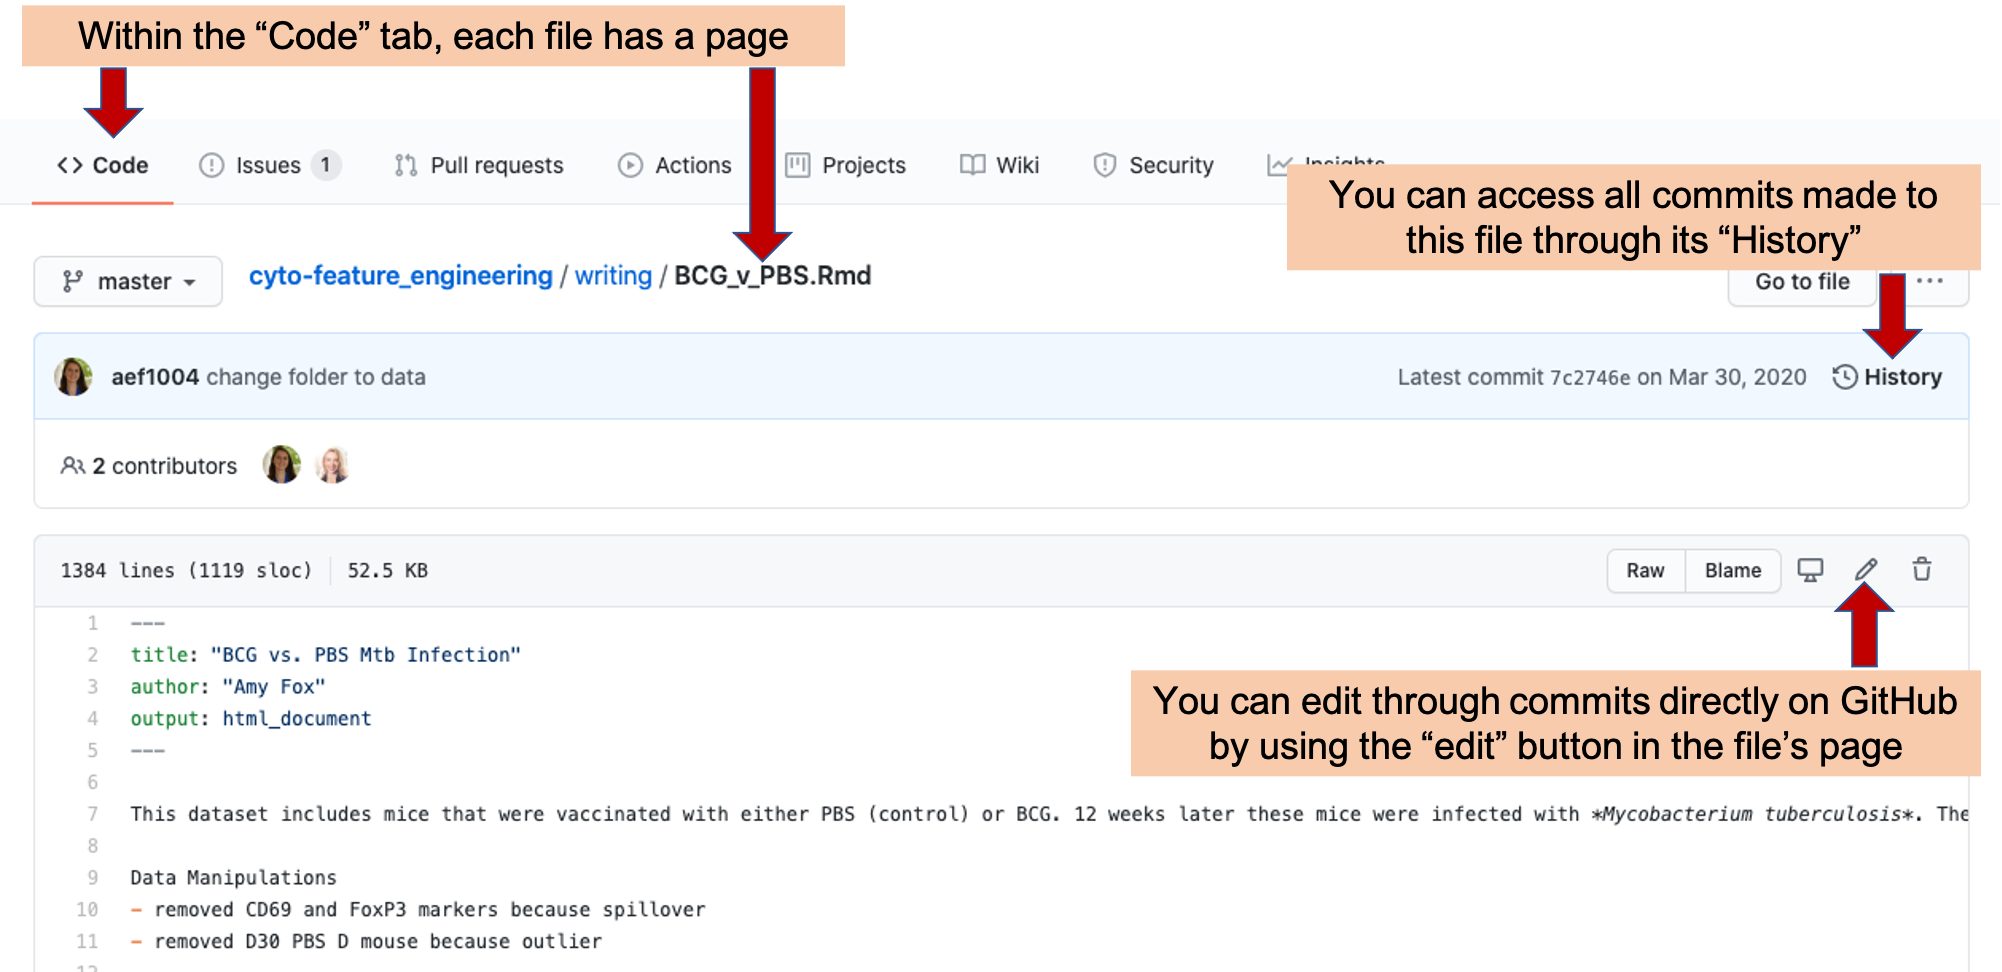
\includegraphics[width=\textwidth]{figures/github_commits1} \caption[Example of a file page within a GitHub repository]{Example of a file page within a GitHub repository. Each file in a repository has its own page. On this page, you can see the history of changes made to the file by looking at 'History'. You can also make a commit an edit directly in GitHub by clicking on the 'Edit' icon.}\label{fig:githubcommits1}
\end{figure*}

Figure \ref{fig:githubcommithistory} gives an example of how you can see the
full history of changes that have been made to each file in the project. Each
change is tracked through a commit, which includes markers of who made the
change and a message describing the change. This allows you to quickly pinpoint
changes in a file in your research project. Near the commit message are listings
of which team member made the commit and when it was made. This also helps you
see how team members have contributed as the file evolves.

\begin{figure*}
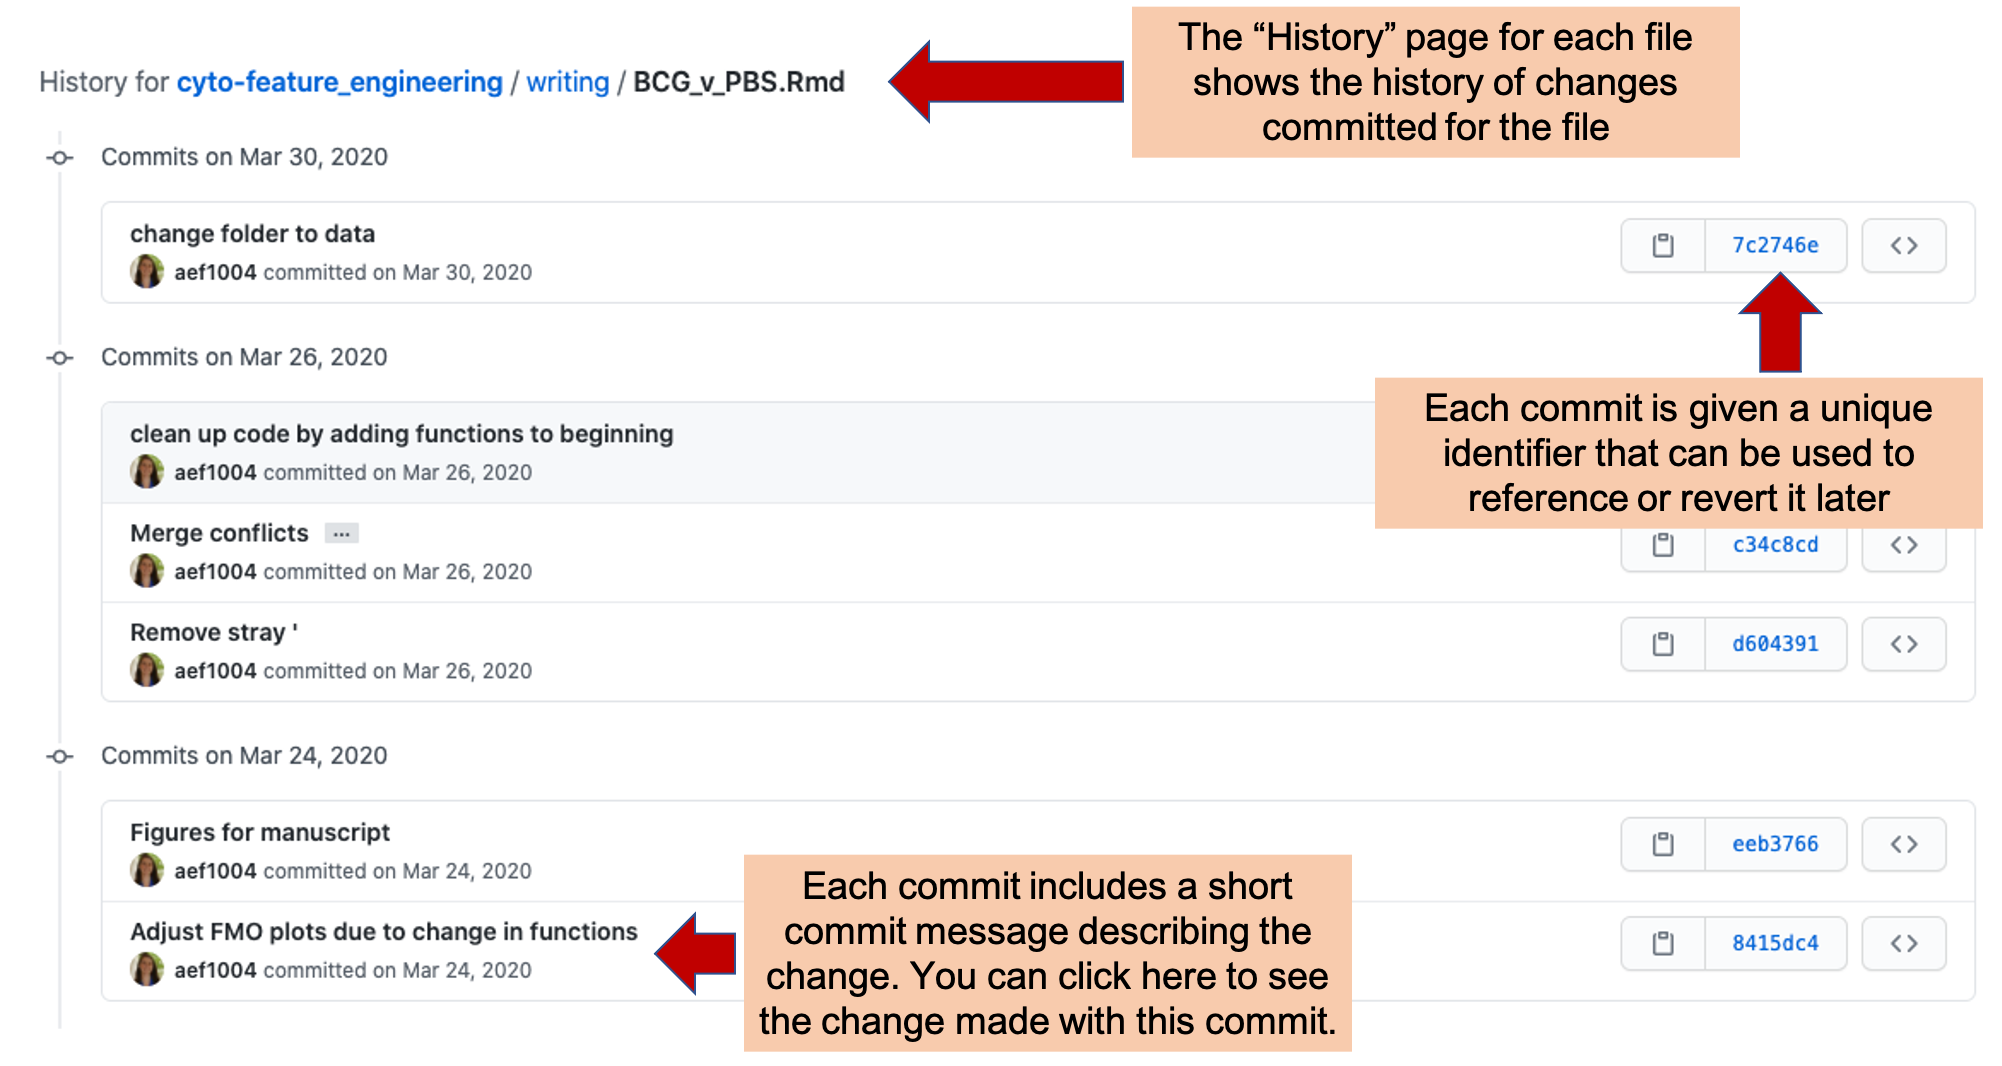
\includegraphics[width=\textwidth]{figures/github_commit_history} \caption[Commit history in GitHub]{Commit history in GitHub. Each file in a repository has a 'History' page, where you can explore each change commited for the file. Each commit has a unique identifier and commit message describing the change. You can click on the entry for any of these commits to see the changes made to the file with the commit (see next figure).}\label{fig:githubcommithistory}
\end{figure*}

If you click on one of the commits listed on a file's History page (Figure
\ref{fig:githubcommithistory} points to one example of where you would click),
it will take you to a page providing information on the changes made with that
commit (Figure \ref{fig:githubcommithistory2}). This page provides a
line-by-line view of each change that was made to project files with that
commit, as well as the commit message for that commit. If the person
committing the change included a longer description or commentary,
this information will also be included.

Within the body of the page, you can see the changes made with the commit. Added
lines will be highlighted in green while deleted lines are highlighted in red.
If only part of a line was changed, it will be shown twice, once in red as its
version before the commit, and once in green showing its version following the
commit. You can visually compare the two versions of the line to see how it was
changed with the commit.

\begin{figure*}
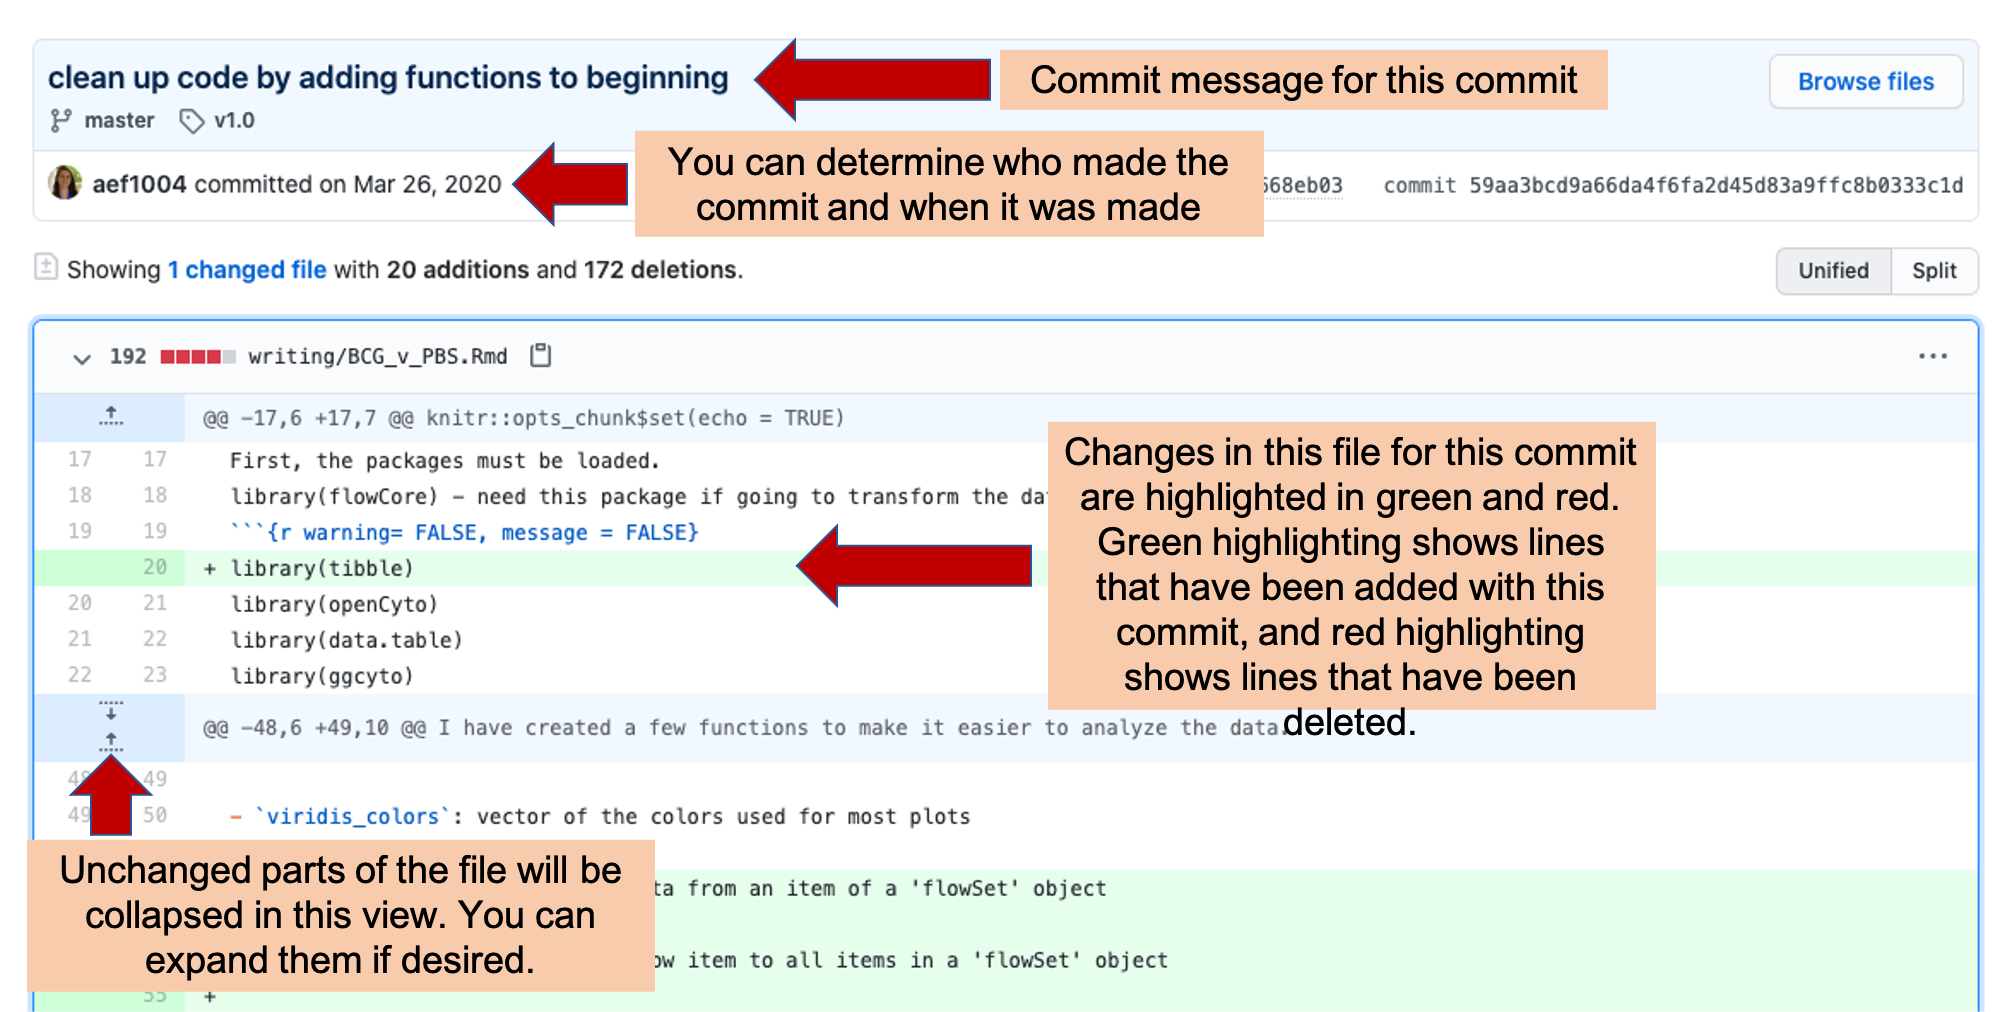
\includegraphics[width=\textwidth]{figures/github_commit_history2} \caption[Commit history in GitHub]{Commit history in GitHub. Each commit has its own page, where you can explore what changes were made with the commit, who made them, and when they were committed.}\label{fig:githubcommithistory2}
\end{figure*}

The page shown in Figure \ref{fig:githubcommits1} also allows you to make your
own edits to the file and commit them. For team members who are working a lot on
coding, they will usually make changes to a file locally, on the repository copy
on their own computers and then push their latest changes to the GitHub version.
This workflow will allow them to test the code locally before they update the
GitHub version.

However, it is also possible to make a commit directly on GitHub, and this may
be a useful option for team members who are not coding and would like to make
small changes to the writing files. On the file's page on GitHub, there is an
``Edit'' icon (Figure \ref{fig:githubcommits1}). By clicking on this, you will
get to a page where you can directly edit the file (Figure
\ref{fig:githubcommits2} shows an example of what this page looks like). Once
you have made your edits, you will need to commit them, along with a short
description of the commit, the ``commit message''. If you would like to include a
longer explanation of your changes, there is space for that, as well, when you
make the commit (Figure \ref{fig:githubcommits2}). These commits will show up
in the repository's history, attributed to you and with your commit message
attached to the change.

\begin{figure*}
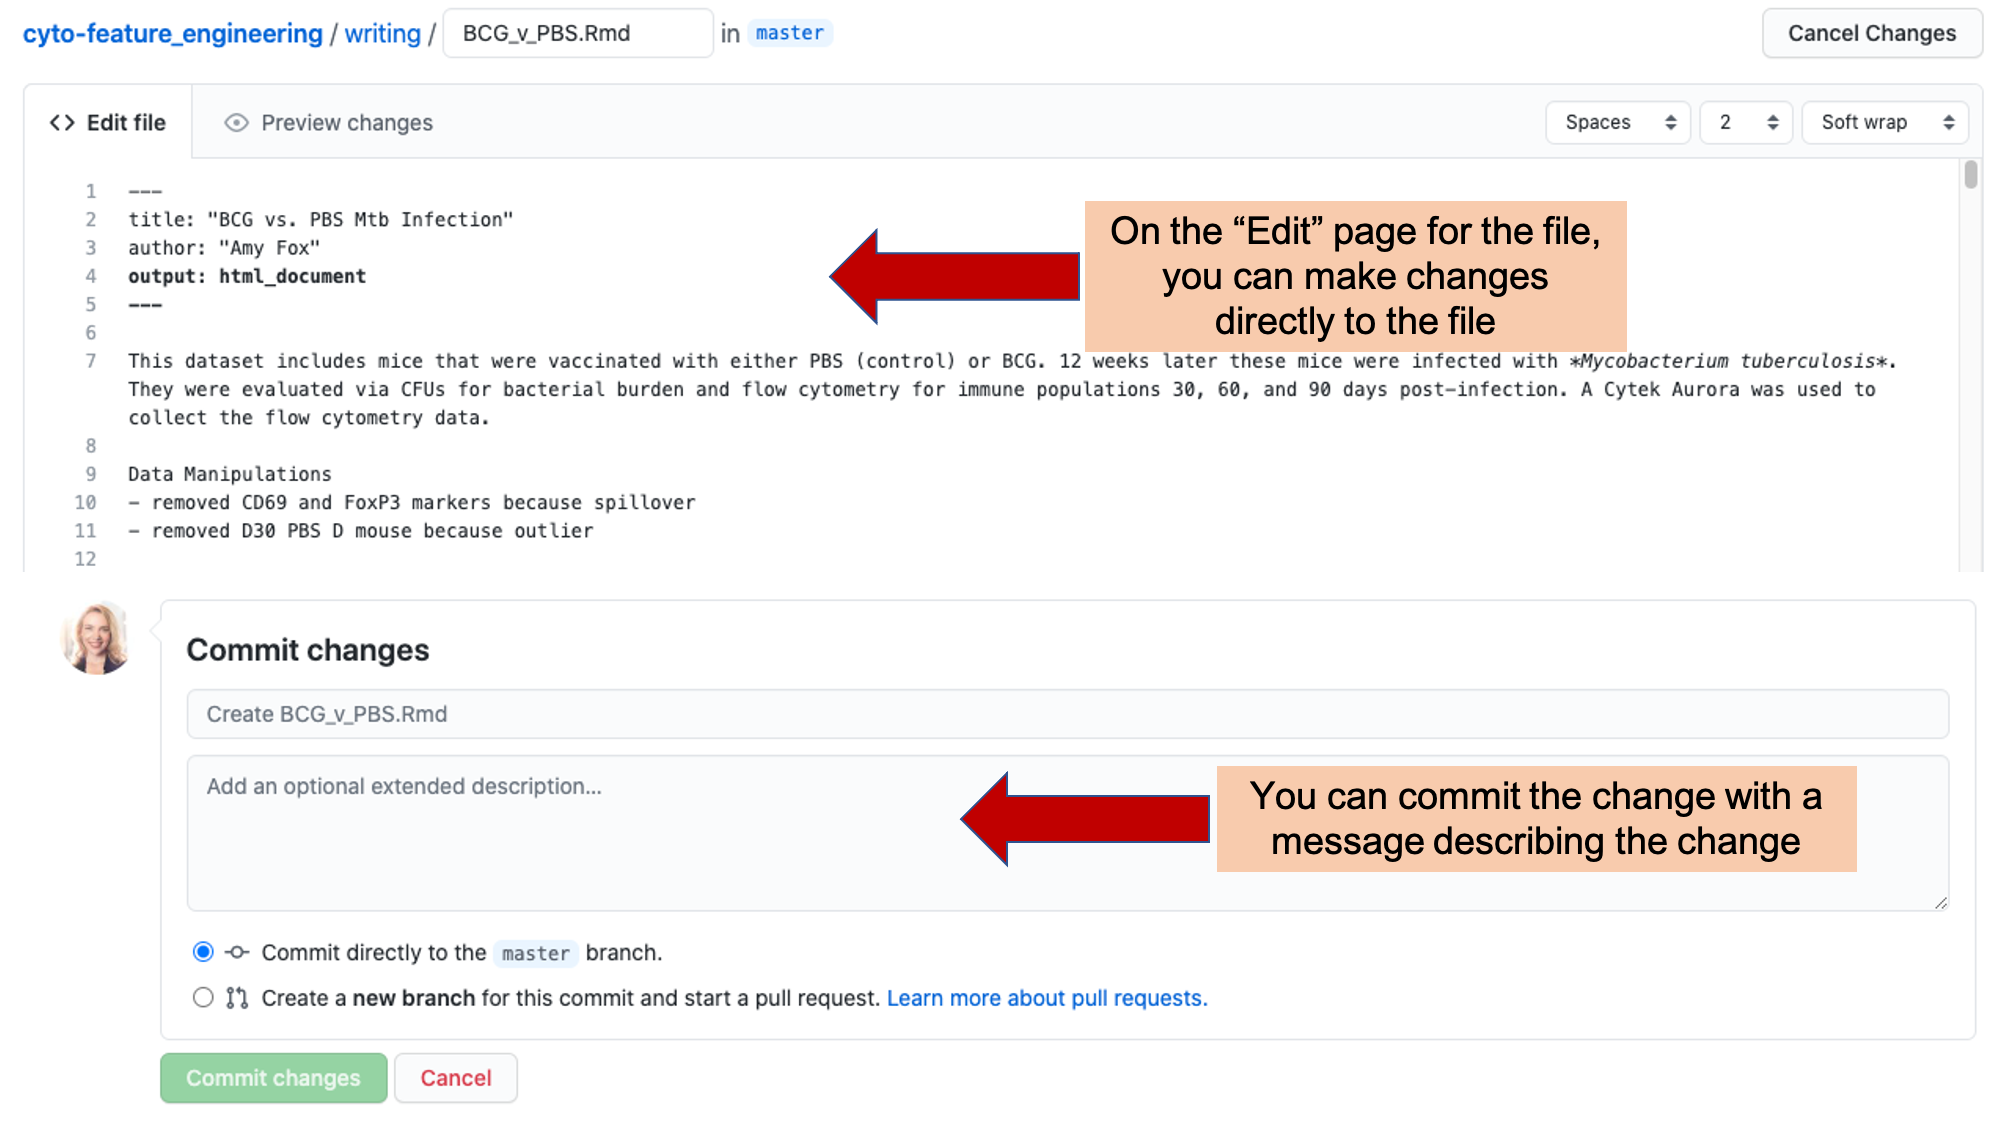
\includegraphics[width=\textwidth]{figures/github_commits2} \caption[Committing changes directly in GitHub]{Committing changes directly in GitHub. When you click on the 'Edit' button in a file's GitHub page (see previous figure), it will take you to a page where you can edit the file directly. You save the changes with a 'commit', including a commit message describing why you made the change. The change will be tagged with the message and your name.}\label{fig:githubcommits2}
\end{figure*}

\textbf{Tracking and making progress on issues}

Another way that a version control platform like GitHub can help you manage a
project is through the ``Issues'' tracker. As we described in module 2.10,
this Issues page can serve as a ``to-do'' list for the project as a whole.
It lets you keep track of the tasks that need to be done, as well as
have detailed conversations with your team about each task.

Each repository includes this type of tracker, and it can be easily used by all
team members, whether they are comfortable coding or not. Figure
\ref{fig:githubissues1} gives an example of \href{https://github.com/aef1004/cyto-feature_engineering/issues}{the Issues tracker
page} for the
repository we are using as an example. There will be a main Issues page, like
one shown in this figure, as well as separate pages for each Issue.

\begin{figure*}
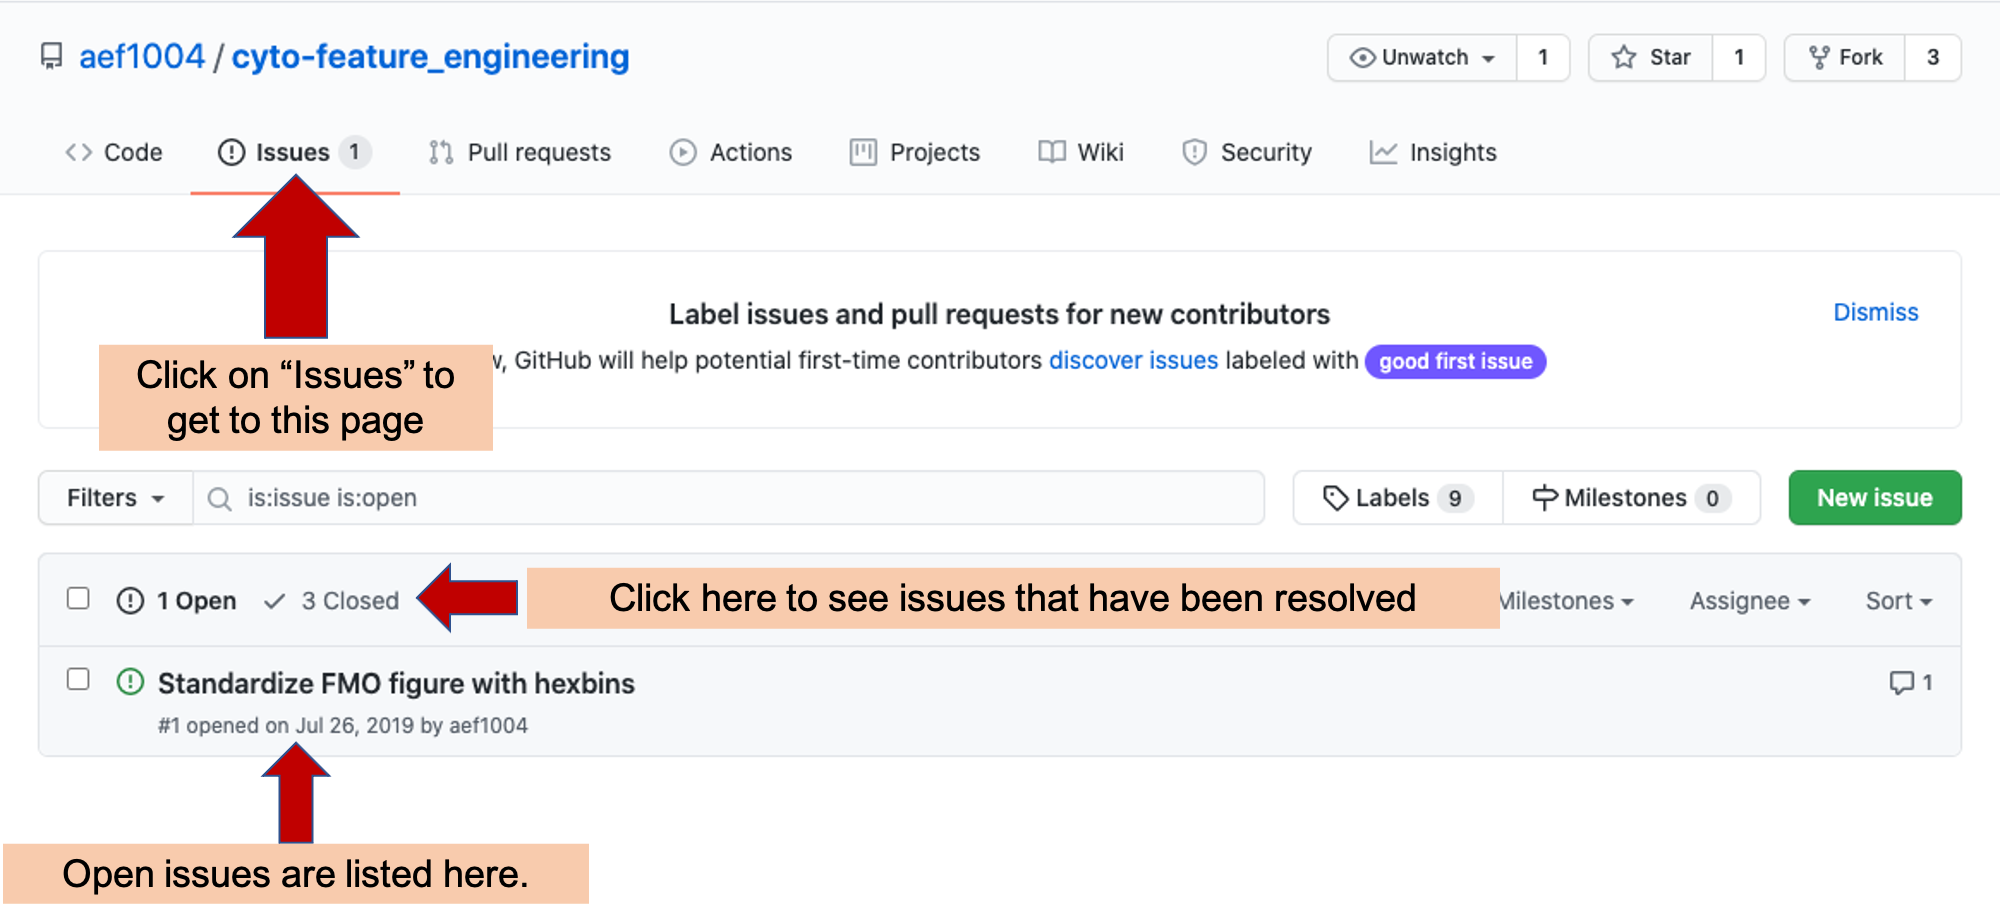
\includegraphics[width=\textwidth]{figures/github_issues} \caption[Issues tracker page for an example GitHub repository]{Issues tracker page for an example GitHub repository. Arrows highlight the tab to click to get to the Issues tracker page in a repository, as well as where to go to find open and closed Issues for the repository.}\label{fig:githubissues1}
\end{figure*}

The main Issues tracker page provides clickable links to all open issues for
the repository. You can open a new issue using the ``New Issue'' on this main
page or on the specific page of any of the repository's issues. See Figure
\ref{fig:githubissues2} for an example of this button.

\begin{figure*}
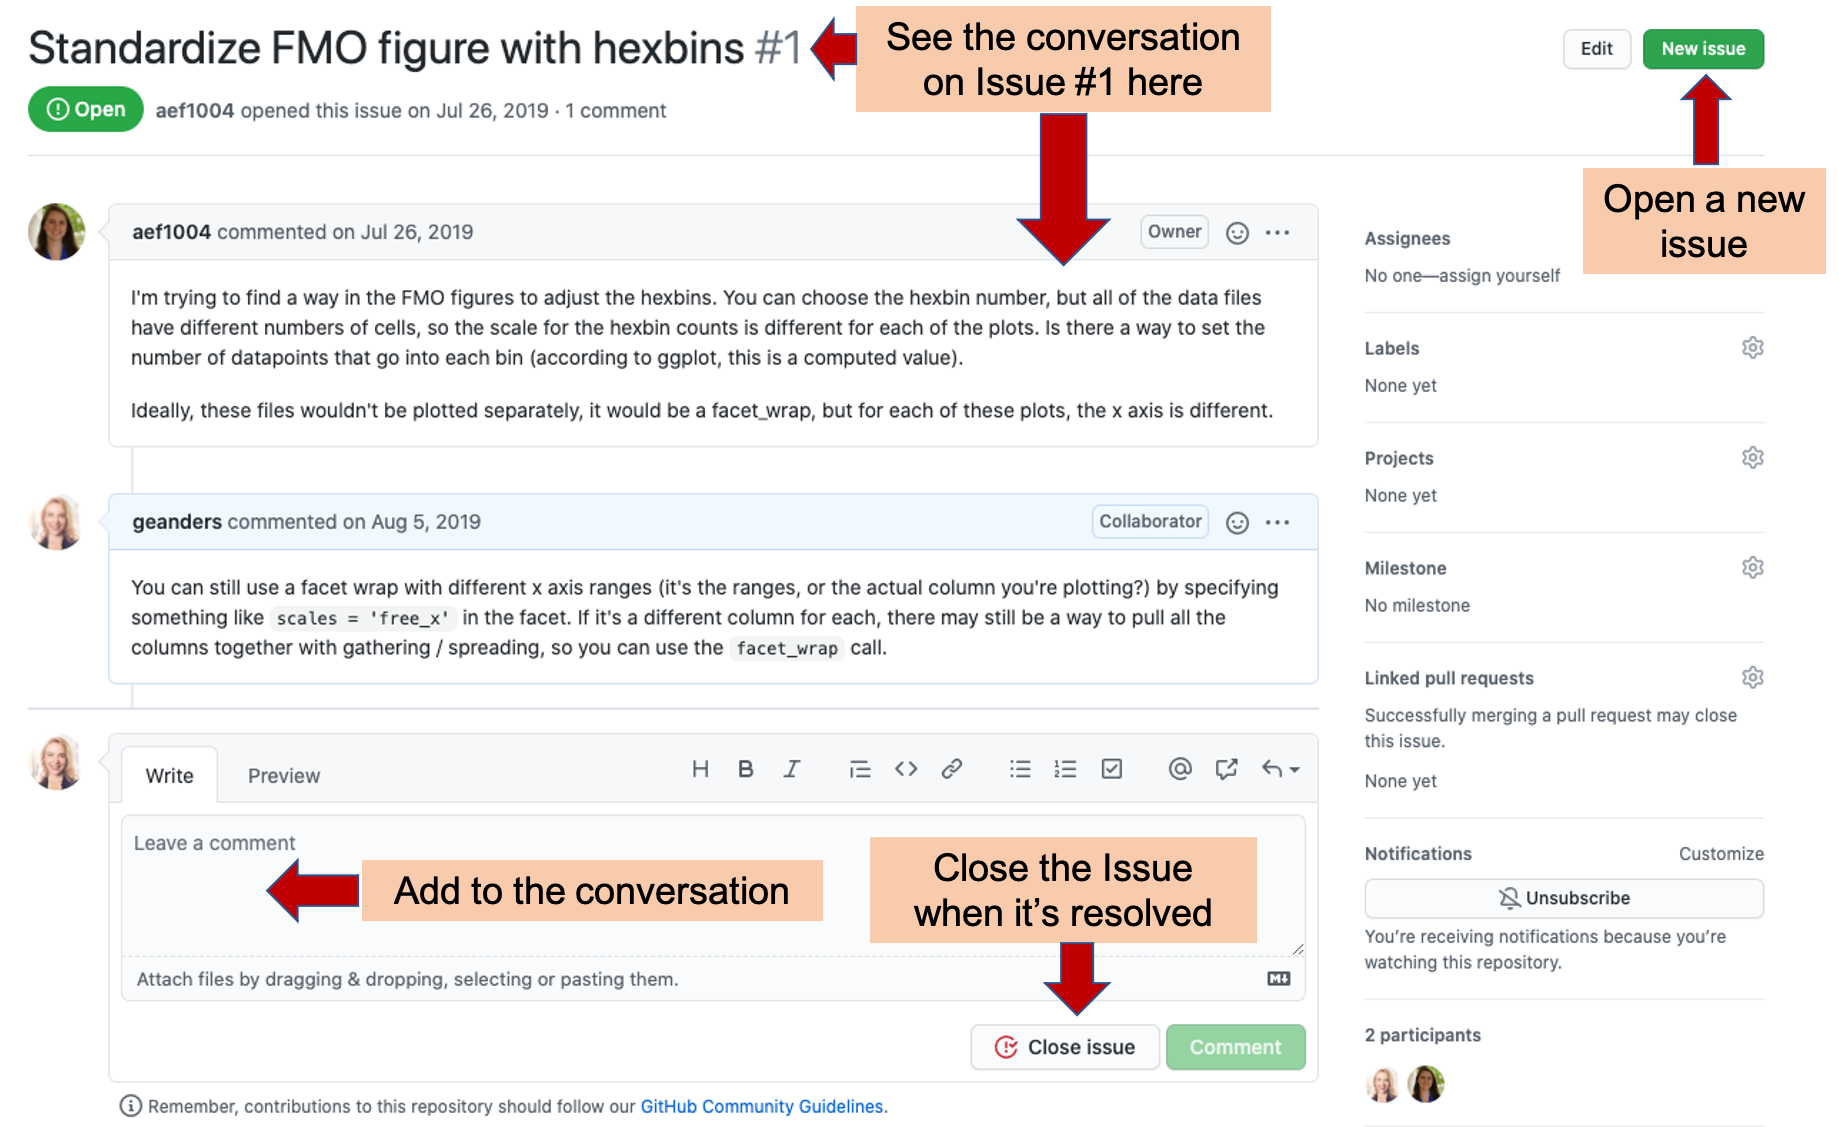
\includegraphics[width=\textwidth]{figures/github_issues2} \caption[Conversation about an Issue on Issues tracker page of an example GitHub repository]{Conversation about an Issue on Issues tracker page of an example GitHub repository. In this example, you can see how GitHub Issues trackers allow you to discuss how to resolve an issue across your team. From this page, you can read the current conversation about Issue \#1 of the repository and add your own comments. Once the Issue is resolved, you can 'Close' the Issue, which moves it off the list of active issues, but allows you to still re-read the conversation and, if necessary, re-open the issue later. You can also open a new issue from this page, using the button highlighted at the top right.}\label{fig:githubissues2}
\end{figure*}

On the page for a specific issue (e.g., Figure \ref{fig:githubissues2}), you
can have a conversation with your team to determine how to resolve the issue.
This conversation can include web links, figures, and even lists with check boxes, to
help you discuss and plan how to resolve the issue. Each issue is numbered,
which allows you to track each individually as you work on the project.

Once you have resolved an issue, you will close it, using a ``Close'' button on the
Issue's page (see Figure \ref{fig:githubissues2} for an example). This moves the issue
from the active list into a ``Closed'' list. Each closed issue still has its
own page, where you can read through the conversation describing how it
was resolved. If you need to, you can re-open a closed issue later, if you
determine that it was not fully resolved. Figure \ref{fig:githubissues1} shows
where to go to see a list of closed Issues for a project.

\begin{figure*}
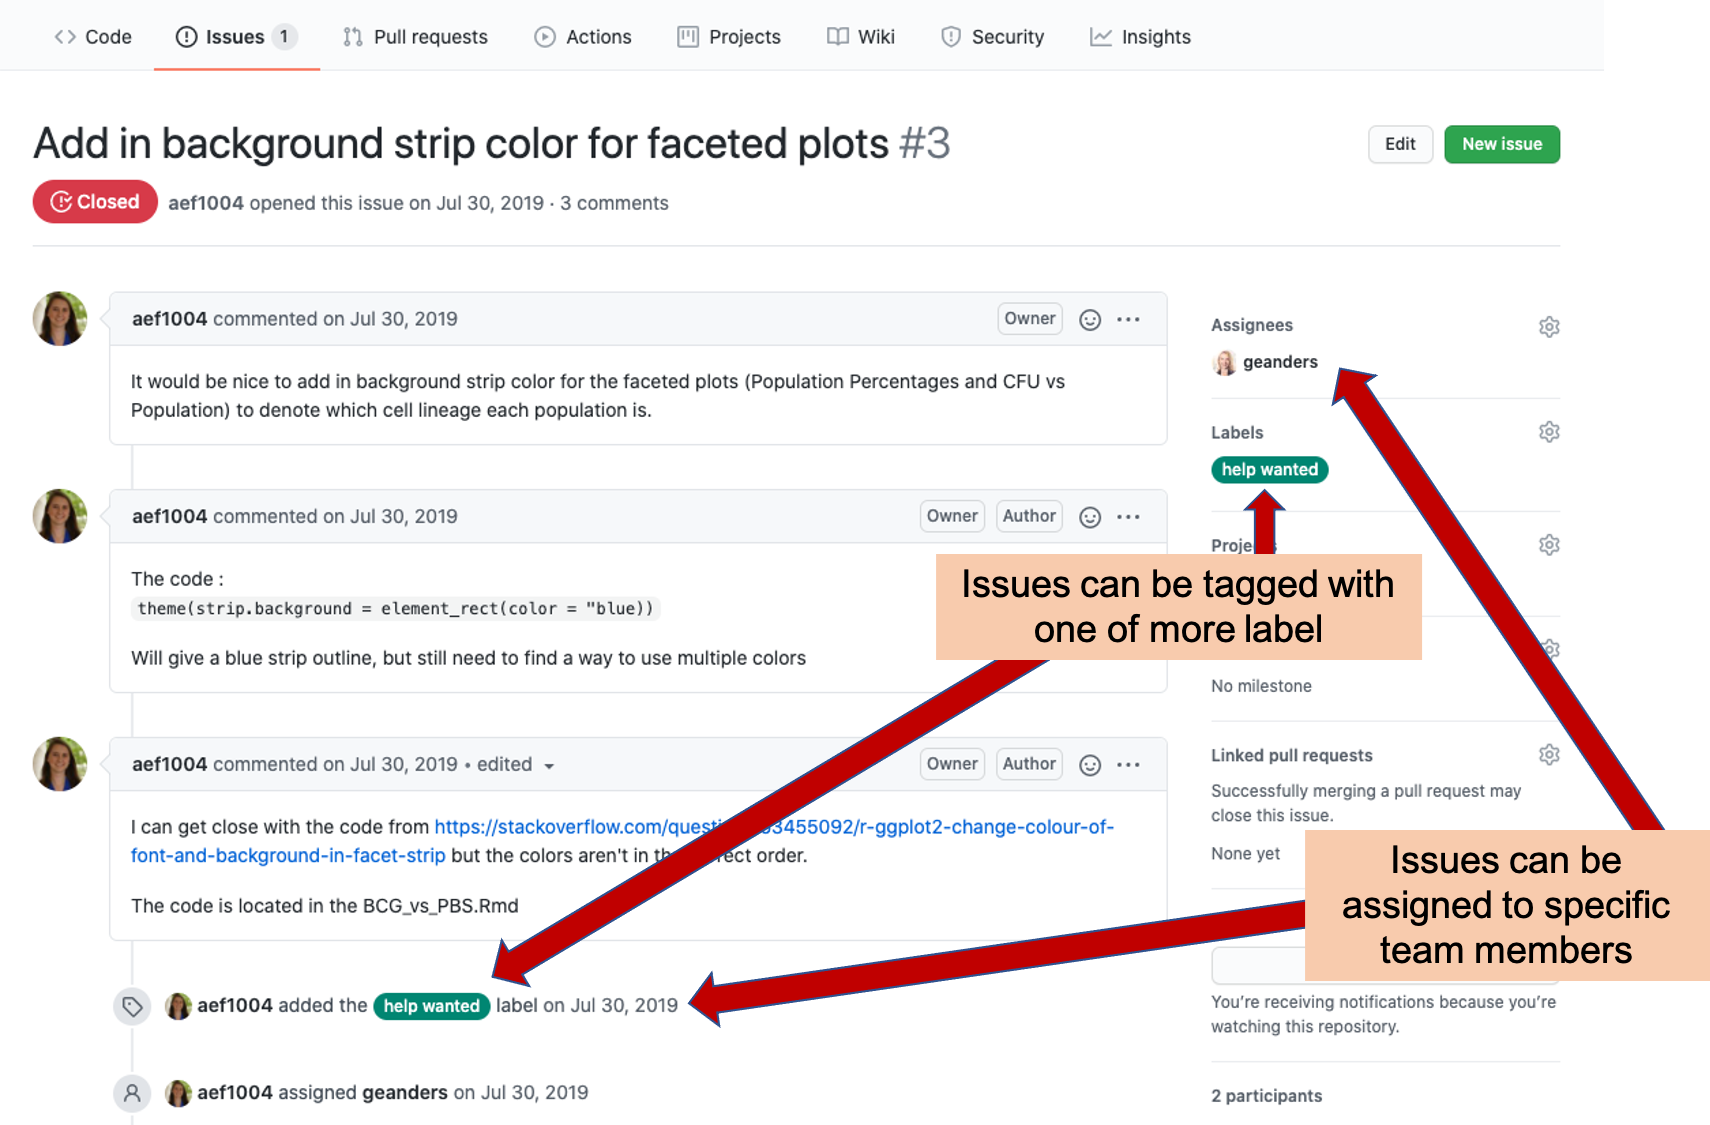
\includegraphics[width=\textwidth]{figures/github_issues3} \caption[Labeling and assigning Issues]{Labeling and assigning Issues. The GitHub Issues tracker allows you to assign each issue to one or more team members, clarifying that they will take the lead in resolving the issue. It also allows you to tag each issue with one or more labels, so you can easily navigate to issues of a specific type or identify the category of a specific issue.}\label{fig:githubissues3}
\end{figure*}

The Issues tracker page includes more advanced functionality, as well
(Figure \ref{fig:githubissues3}). For example, you can assign an issue to one
of more team members, indicating that they are responsible for resolving that
issue. You can also tag each issue with one of more labels, allowing you to
group issues into common categories. For example, you could tag all issues that
cover questions about pre-processing the data using a ``pre-processing'' label,
and all that are related to creating figures for the final manuscript with a
``figures'' label.

\textbf{Managing repository access and ownership}

Repositories include functionality for inviting team members, assigning
roles, and otherwise managing access to the repository. First, a repository
can be either public or private. For a public repository, anyone will be
able to see the full contents of the repository through GitHub. You can
also set a repository to be private. In this case, the repository can only
be seen by those who have been invited to collaborate on the repository, and
only when they are logged in to their GitHub accounts. The private / public
status of a repository can be changed at any time, so if you want you can
maintain a repository for a project as private until you publish the results,
and then switch it to be public, to allow others to explore the code and data
that are linked to your published results.

You can invite team members to collaborate on a repository, as long as they have
GitHub accounts. While public repositories can be seen by anyone, the only
people who can add to or change the contents of the repository are people who
have been invited to collaborate on the repository. The person who creates the
repository (the repository ``owner'') can invite other collaborators through the
``Settings'' tab of the repository, which will have a ``Manage access'' function for
the repositories maintainer. Only the owner of the repository will have access
to this tab for the repo. On this page, you can invite other collaborators by
searching using their GitHub ``handle'' (the short name they chose to be
identified by in GitHub). You can also change access rights, for example,
allowing some team members to be able to make major changes to the
repository---like deleting it---while others can make only smaller
modifications.

{[}Add: Roles on a repository{]}

If you are the owner of a repository, or have administrator rights on an
organization repository, you will have access to an additional page for the
repository---the ``Settings'' page. Figure \ref{fig:githubsettings} shows
the tab that you'll click on to access this Settings page. (If you do
not see this tab when you're exploring a repository, you either do not have
owner-level rights for that repository or you aren't logged in to your GitHub
account.)

\begin{figure*}
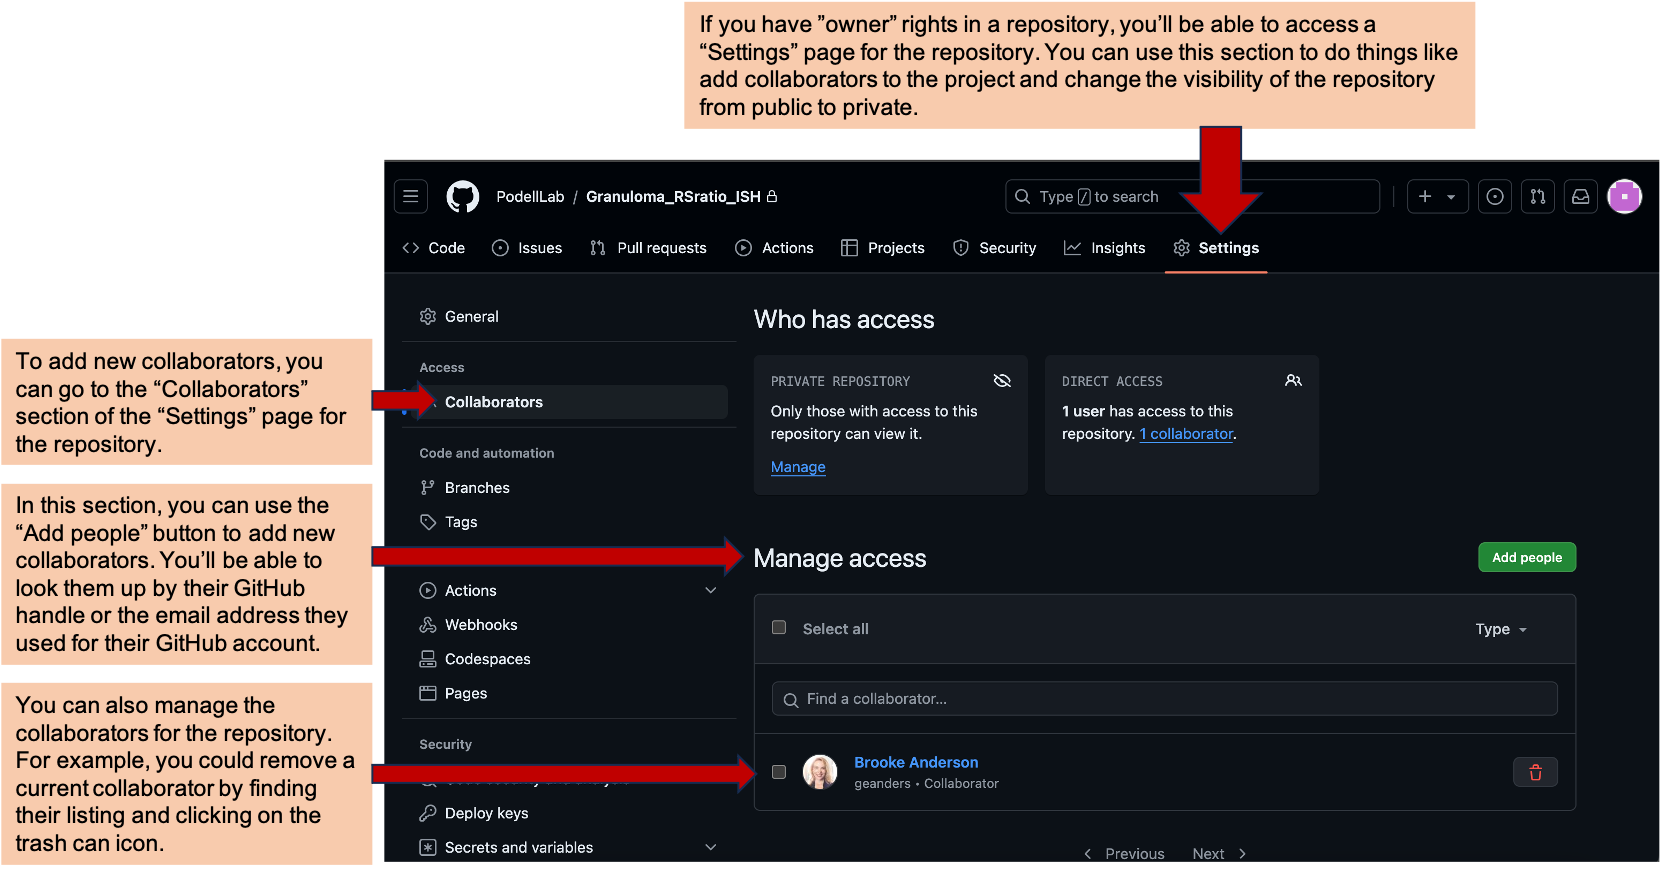
\includegraphics[width=\textwidth]{figures/github_settings} \caption[If you have owner-level rights to a repository, you will have access to an additional page on the repository, called 'Settings']{If you have owner-level rights to a repository, you will have access to an additional page on the repository, called 'Settings'. You can use this page for several administrative tasks for the repository. For example, you can add or remove collaborators for the repository.}\label{fig:githubsettings}
\end{figure*}

You can use the Settings page to manage the collaborators for the project.
If you go to the ``Collaborators'' section of the Settings page
(Figure \ref{fig:githubsettings}), you can add new collaborators using the
``Add people'' button. This will allow you to search for a new collaborator
using either their GitHub handle or the email they used to set up their
GitHub account. Once you invite someone, they will get an email invitation,
and they can respond to that invitation to join as a collaborator on the
repository. You can also use this area to manage people who are already
collaborators. For example, if you need to remove a collaborator from the
project, you can do that in this ``Collaborators'' section of the Settings
page for the repository.

If you are the owner of a repository (or have administrative rights on an
organization-style repository), you will be able to change the repository
visibility, toggling it between private and public or vice-versa. You'll do
this on the Settings page of the repository. If you scroll down that page,
you'll get to an area called the ``Danger Zone'', as shown in
Figure \ref{fig:githubpublicprivate}. In this section, there's a line labeled
``Change repository visibility''. Here you can click on a button to ``Change
visibility''. If the repository is currently private, this brings up the option to
``Change to public''. Once you click this, anyone will be able to view that
repository using the repository's web link. If you are using the repository
for a paper, you could use this functionality to change the repository from
private---while you're working on the paper---to public---once you've
published the paper and want to share the code and data.

\begin{figure*}
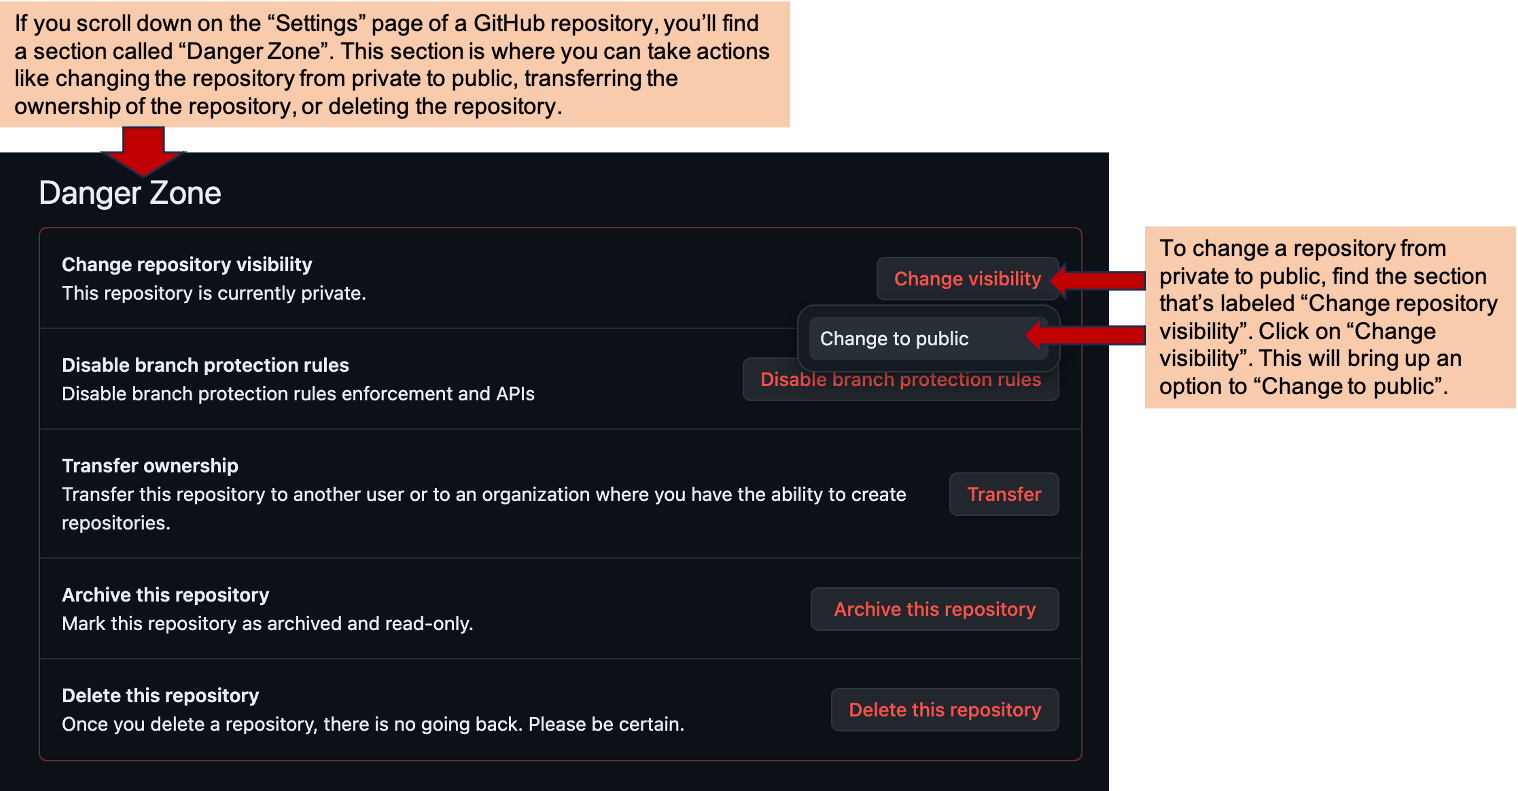
\includegraphics[width=\textwidth]{figures/github_public_private} \caption[If you have owner-level rights for a repository, you can change the visibility of the repository]{If you have owner-level rights for a repository, you can change the visibility of the repository. To do this, go to the 'Settings' page of the repository and scroll down to the 'Danger Zone' section, shown here. In this section, you can change the repository from private to public using the option to 'Change repository visibility'.}\label{fig:githubpublicprivate}
\end{figure*}

\textbf{Providing project documentation}

{[}Add: README with Markdown{]}

If you are planning to use GitHub as a way to share the project directory, you
will find it useful to create the README file using a file format called
``Markdown''. {[}Automatically renders in a nice format when you put it on GitHub{]}

\begin{itemize}
\tightlist
\item
  Module 2.7: metadata, README
\item
  Markdown renders nicely when posted on GitHub
\item
  Show example from Amy's project
\end{itemize}

\subsection{Leveraging Git and GitHub as a scientist who programs}\label{leveraging-git-and-github-as-a-scientist-who-programs}

To be able to leverage GitHub to manage projects and share data, you will need
to have at least one person in the research group who can set up the initial
repository. GitHub repositories can be created very easily starting from an
RStudio Project, a format for organizing project files that was described in
module 3.7.

There are many excellent resources that provide instructions on this topic
meant for researchers who are comfortable with using R and RStudio. An
excellent place to start is with an online book written by Jenny Bryan
named \emph{Happy Git and GitHub for the useR}. This book is available for free
at \url{https://happygitwithr.com/}. It provides a gentle yet thorough introduction
to using Git, connecting it to RStudio Projects, and connecting everything
with an online version control platform like GitHub. It also includes a
helpful section that covers what a daily workflow will look like when you
are using Git and GitHub in conjunction with projects that include R code.

Once you've explored that resource, some others you might find useful are:

\begin{itemize}
\tightlist
\item
  Software Carpentry's introduction to version control with Git, available at
  \url{https://swcarpentry.github.io/git-novice/}
\item
  Article on \href{https://journals.plos.org/ploscompbiol/article?id=10.1371/journal.pcbi.1004668}{\emph{A Quick Introduction to Version Control with Git and GitHub}}
  \citep{blischak2016quick}
\item
  Article on \href{https://journals.plos.org/ploscompbiol/article?id=10.1371/journal.pcbi.1004947}{Ten Simple Rules for Taking Advantage of Git and GitHub}
  \citep{perez2016ten}
\end{itemize}

\chapter{Experimental Data Pre-processing}\label{experimental-data-pre-processing}

This section includes modules on:

\begin{itemize}
\tightlist
\item
  \hyperref[module12]{Module 3.1: Principles of pre-processing experimental data}
\item
  \hyperref[module12a]{Module 3.2: Selecting software options for pre-processing}
\item
  \hyperref[module13]{Module 3.3: Introduction to scripted data pre-processing in R}
\item
  \hyperref[module13a]{Module 3.4: Tips for improving reproducibility when writing R scripts}
\item
  \hyperref[module14]{Module 3.5: Simplify scripted pre-processing through R's `tidyverse' tools}
\item
  \hyperref[module15]{Module 3.6: Complex data types in experimental data pre-processing}
\item
  \hyperref[module18]{Module 3.7: Introduction to reproducible data pre-processing protocols}
\item
  \hyperref[module19]{Module 3.8: RMarkdown for creating reproducible data pre-processing protocols}
\item
  \hyperref[module20]{Module 3.9: Example: Creating a reproducible data pre-processing protocol}
\end{itemize}

\section{Principles of pre-processing experimental data}\label{module12}

The experimental data collected for biomedical research often requires
pre-processing before it can be analyzed. In any scientific field, when you work
with data, it will often take much more time to prepare the data for analysis
than it takes to set up and run the statistical analysis itself
\citep{robinson2014broom}. This is certainly true with complex biomedical data,
including data for flow cytometry, transcriptomics, proteomics, and
metabolomics. It is a worthwhile investment of time to learn strategies to make
pre-processing of this data more efficient and reproducible, and it is
critical---for the rigor of the entire experiment---to ensure that the
pre-processing is done correctly and can be repeated by others.

These pre-processing steps, in fact, should be as clear and practical to follow
as the types of protocols you would follow for a wet lab procedure. Key to
reproducibility is that a procedure is described in enough detail that others
can follow it exactly. Use of point-and-click software and/or propritary
software can limit the transparency and reproducibility of this analysis stage
and is time-consuming for repeated tasks.

In this module, we will explain how pre-processing can be broken into common
themes and processes. In the next module, we will explain how scripted
pre-processing, especially using open-source software, can improve transparency
and reproducibility of this stage of working with biomedical data.

\textbf{Objectives.} After this module, the trainee will be able to:

\begin{itemize}
\tightlist
\item
  Define ``pre-processing'' of experimental data, ``noise'' in data, ``batch effects'',
  ``normalization'', ``dimension reduction'', and ``feature selection''
\item
  List some reasons that pre-processing might be necessary
\item
  Understand key themes and processes in pre-processing and identify these
  processes in their own pipelines
\end{itemize}

\subsection{What is data pre-processing?}\label{what-is-data-pre-processing}

When you are conducting an experiment that involves work in the wet lab, you
will do a lot of work before you have any data ready for analysis. You may,
for example, have conducted an extensive amount of work that involved laboratory
animals or cell cultures. In many cases, you will have run some samples through
very advanced equipment, like cytometers or sequencers. Once you have completed
this long and hard process, you may ask yourself, ``I ran the experiment, I ran
the equipment\ldots{} Aren't I done with the hard work?''.

For certain types of data, you may be, and you may be able to proceed directly to
statistical analysis. For example, if you collected the weights of lab animals,
you are probably directly using those data to answer questions like whether weight
differed between treatment groups. However, with a lot of biomedical data, you
will not be able to move directly to analyzing the data. Instead, you will need
to start with a stage of \emph{pre-processing} the data: that is, taking
computational steps to prepare the data before it's in an appropriate format to
be used in statistical analysis.

There are several reasons that pre-processing is often necessary. The first is
that many biomedical data are collected using extremely complex equipment and
scientific principles. The pre-processing in this case is used to extract scientific
meaning from data that might have been collected using measurements that are
more closely linked to the complex process than to the final scientific question.
Next, there will be some cases where practical concerns made it easier to
collect data in one way and pre-process it later to get it to a format that
aligns with the scientific question. For example, if you want the average weight
of mice in different treatment groups, it may be more practical to weigh the
cage that contains all the mice in each treatment group rather than weigh
each mouse individually. This makes life in the lab easier, but means you'll need
to do some more computational pre-processing of the data to make sense of it
later. Third, there are now frequent cases where an assay generates
a very large set of measures---for example, expression levels of thousands of
genes for each sample---and some pre-processing might help in digesting the
complexity inherent in this type of high-dimensional data. Finally, pre-processing
is often necessary to check for and resolve quality control issues within the
data. In this module, we'll explore each of these themes of pre-processing in
more depth.

\subsection{Common themes and processes in data pre-processing}\label{common-themes-and-processes-in-data-pre-processing}

Exactly what pre-processing you will need to do will vary depending on the way the data
were collected and the scientific questions you hope to answer, and often it
will take a lot of work to develop a solid pipeline for pre-processing data from
a specific assay. However, there are some common themes that drive the need for
such pre-processing of data across types of data collection and research
questions. These common themes provide a framework that can help as you design
data pre-processing pipelines, or as you interpret and apply pipelines that were
developed by other researchers. The rest of this module will describe several of
the most common themes in data pre-processing.

\textbf{Extracting scientifically-relevant measurement}

One common purpose of pre-processing is to translate the measurements that
you directly collect into measurements that are meaningful for your scientific
research question. Scientific research uses a variety of complex techniques and
equipment to initially collect data. As a result of these inventions and
processes, the data that are directly collected in the laboratory by a person or
piece of equipment might require quite a bit of pre-processing to be translated
into a measure that meaningfully describes a scientific process. A key element
of pre-processing data is to translate the acquired data into a format that can
more directly answer scientific questions.

This type of pre-processing will vary substantially from assay to assay, with
algorithms that are tied to the methodology of the assay itself. We'll describe
some examples of this idea, moving from an example of a very simple translation
to processes that are much more complex (and more typical of the data collected
at present in many types of biomedical research assays).

As a basic example, some assays use equipment that can measure the
intensity of color of a sample or the sample's opacity. Some of these measures
might be directly (or at least proportionally) interpretable. For example,
opacity might provide information about the concentration of bacteria
in a sample. Others might need more interpretation, based on the scientific
underpinnings of the assay. For example, in an enzyme-linked immunosorbent assay
(ELISA), antibody levels are detected as a measure of the intensity of color of
a sample at various dilutions, but to interpret this correctly, you need to know
the exact process that was used for that assay, as well as the dilutions that
were measured.

The complexity of this ``translation'' scales up as you move to data that are
collected using more complex processes. Biomedical research today leverages
extraordinarily complex equipment and measurement processes to learn more about
health and disease. These invented processes of measuring can
provide detailed and informative data, allowing us to ``see''
elements of biological processes that could not be seen at that level before.
However, they all require steps to translate the data that are directly
recorded by equipment into data that are more scientifically meaningful.

One example is flow cytometry. In flow cytometry, immune cells are characterized
based on proteins that are present both within and on the surface of each cell,
as well as properties like cell size and granularity \citep{maecker2012standardizing, barnett2008cd4}. Flow cytometry identifies these proteins through a complicated
process that involves lasers and fluorescent tags and that leverages a key
biological process---that an antibody can have a very specific affinity for one
specific protein \citep{barnett2008cd4}.

The process starts by identifying proteins that can help to
identify specific immune cell populations (e.g., CD3 and CD4 proteins in
combination can help identify helper T cells). This collection of proteins is
the basis of a panel that's developed for that flow cytometry experiment. For
each of the proteins on the panel, you will incorporate an antibody with a
specific affinity for that protein. If that antibody sticks to the cell in a
substantial number, it indicates the presence of its associated protein on the
cell.

To be able to measure which of the antibodies stick to which cells, each type of
antibody is attached to a specific fluorescent tag (each of these is often
referred to as a ``color'' in descriptions of flow cytometry) \citep{benoist2011flow}.
Each fluorescent tag included in the panel will emit wavelength in a certain
well-defined range after it is exposed to light at wavelengths of a certain
range. As each cell passes through the flow cytometer, lasers activate these
fluorescent tags, and you can measure the intensity of light emitted at specific
wavelengths to identify which proteins in the panel are present on or in each
cell \citep{barnett2008cd4}.

This is an extraordinarily clever way to identify cells, but the complexity of
the process means that a lot of pre-processing work must be done on the resulting
measurements. To interpret the data that are recorded by a flow cytometer
(intensity of light at different wavelengths)---and to generate a
characterization of immune cell populations from these data---you need to
incorporate a number of steps of translation. These include steps that
incorporate information about which fluorescent tags were attached to which
antibodies, which proteins in the cell each of those antibodies attach to, which
immune cells those proteins help characterize, what wavelength each fluorescent
tag emits at, and so on. In some cases, the measuring equipment will provide
software that performs some of this pre-processing before you get the first
version of the data, but some may need to be performed by hand, especially if
you need to customize based on your research question. Further, it's critical to
understand the process, to decide if it's appropriate for your specific
scientific question.

Similarly complex processes are used to collect data for many single-cell and
high throughput assays, including transcriptomics, metabolomics, proteomics,
and single cell RNA-sequencing. It can require complex and sometimes lengthy
algorithms and pipelines to extract direct scientifically-relevant measures
from the measures that the laboratory equipment captures in these cases.
Depending on the assay, this pre-processing can include sequence alignment
and assembly (if sequencing data were collected) or peak identification and
alignment (if data was collected using mass spectrometry, for example).

As Paul Flicek and Ewan Birney note in an article on making sense of
sequence reads:

\begin{quote}
``The individual outputs of the sequence machines are essentially worthless by
themselves. \ldots{} Fundamental to creating biological understanding from the
increasing piles of sequence data is the development of analysis algorithms able
to assess the success of the experiments and synthesize the data into manageable
and understandable pieces.'' \citep{flicek2009sense}
\end{quote}

The discipline of bioinformatics works to develop these types of pre-processing
algorithms \citep{barry2009new}. Many of them are available through open-source,
scripted software like R and Python. These types of pre-processing algorithms
are often also available as proprietary software, sometimes sold by equipment
manufacturers and sometimes separately.

\textbf{Addressing practical concerns and limitations in data collection}

Another common reason for pre-processing is to address things you
did while collecting the data---specifically, things you did for
practical purposes or under practical limitations. These will then need to
be handled, when possible, in computational pre-processing.

This type of pre-processing often addresses something called
\emph{noise} in the data. When we collect biomedical
research data, we are collecting it in the hope that it will measure
some meaningful biological variation between two or more conditions. For
example, we may measure it in the hope that there is a meaningful difference in
gene expression between a sample taken from an animal that is diseased versus
one that is healthy, with the aim of finding a biomarker of the disease.

There are, however, several sources of variation in data we collect. The first
of these is variation that comes from meaningful biological variation between
samples---the type of variation that we are trying to measure and
use to answer scientific questions. We often call this the ``signal'' in the
data \citep{chatfield1995problem}.

There are other sources of variation, too, though. These sources are irrelevant to
our scientific question, and so we often call them ``noise''---in other words,
they cause our data to change from one sample to the next in a way that might
blur the signal that we care about. We therefore often take steps in
pre-processing to try to limit or remove this type of variation, so we can see the
meaningful biological variation more clearly.

There are two main sources of this noise: biological and technical. Biological
noise in data does come from biological processes, but from ones that are
irrelevant to the process that we care about in our particular experiment. For
example, cells express different genes depending on where they are in the cell
cycle. However, if you are trying to use single cell RNA-sequencing to explore
variation in gene expression by cell type, you might consider this
growth-related variation as noise, even though it represents a biological
process.

The second source of noise is technical. Technical noise comes from variation
that is introduced in the process of collecting data, rather than from
biological processes. In the introduction to the module, we brought up the
example of weighing mice by cage rather than individually; one example of
technical noise in this case would be the differences across the samples that's
based on the number of mice in each cage.

As another example, part of the process of single-cell RNA-sequencing involves
amplifying complementary DNA that are developed from the messenger RNA in each
cell in the sample. How much the complementary DNA are amplified in this
process, however, varies across cells \citep{perkel2017single}. This occurs because,
while the different fragments are all amplified before their sequences are read,
some fragments are amplified more times than others. If two fragments had the
exact same abundence in the original cell, but one was amplified more than the
other, that one would be measured as having a higher level in the sample if this
amplification bias were not accounted for. If this isn't addressed in
pre-processing, amplification bias prevents any meaningful comparison
across cells.

Another source of technical noise is something called \emph{batch effects}. These
occur when data have consistent differences based on who was doing the
measuring, which batch the sample was run with, or which equipment was used for
the measure. For example, if two researchers are working to weigh the mice for
an experiment, the weights recorded by one of the researchers might tend to be,
on average, lower than those recorded by the other researcher, perhaps because
the two scales they are using are calibrated a bit differently. Similarly,
settings or conditions can change in subtle ways between different runs on a
piece of equipment, and so the samples run in different batches might have some
differences in output based on the batch.

In some cases, there are ways to reduce some of the variation that comes from
processes that aren't of interest for your scientific question, either from
biological or technical sources. This is important to consider doing, because
while some of this variation might just lower the statistical power of the
analysis, some can go further and bias the results.

Batch effects, for example, can often be addressed through statistical modeling,
as long as they are identified and are not aligned with a difference you are
trying to measure (in other words, if all the samples for the control animals
are run in one batch and all those for the treated animals in another batch, you
would not be able to separate the batch effect from the effect of treatment).

There are some methods that adjust for batch effects by fitting a regression
model that includes the batch as a factor, and then using the residuals from
that model for the next steps of analysis (``regressing out'' those batch effects)
\citep{mccarthy2017scater}. You can also incorporate this directly into a statistical
model that is being used for the main statistical hypothesis testing of interest
\citep{mccarthy2017scater}. In this case, the technical noise isn't addressed
during the pre-processing phase, but rather as part of the statistical analysis.

Another example of a process that can help adjust for unwanted variation is
normalization. Let's start with a very simple example to explain what
normalization does. Say that you wanted to measure the height of three people,
so you can determine who is tallest and who is shortest. However, rather than
standing on an even surface, they are all standing on top of ladders that are
different heights. If you measure the height of the top of each person's head
from the ground, you will not be able to compare their heights correctly,
because each has the height of their ladder incorporated into the measure. If
you knew the height of each person's ladder, though, you could normalize your
measure by subtracting each ladder's height from the total measurement, and then
you could meaningfully compare the heights to determine which person is tallest.

Normalization plays a similar role in pre-processing many forms of biomedical
data. One article defines normalization as the, ``process of accounting for, and
possibly removing, sources of variation that are not of biological interest''
\citep{mak2011john}. One simple example is when comparing the weights of two groups
of mice. Often, a group of mice might be measured collectively in their cage,
rather than taken out and weighed individually. Say that you have three treated
mice in one cage and four control mice in another cage. You can weigh both cages
of mice, but to compare these weights, you will need to normalize the
measurement by dividing by the total number of mice that are in each cage (in
other words, taking the average weight per mouse). This type of averaging is a
very simple example of normalizing data.

Other normalization pre-processing might be used to adjust for sequencing depth
for gene expression data, so that you can meaningfully compare the measures of a
gene's expression in different samples or treatment groups.
This can be done in bulk RNA sequencing by calculating and adjusting for a
global scale factor \citep{bacher2017scnorm}. One article highlights the critical
role of normalization in RNA sequencing in the context of reproducibility:

\begin{quote}
``The biggest, the easiest way {[}for a biologist doing RNA-Seq to tell that
better normalization of the data is needed{]}---the way that I discovered the
importance of normalization in the microarray context---is the lack of
reproducibility across different studies. You can have three studies that are
all designed to study the same thing, and you just see basically no
reproducibility, in terms of differentially expressed genes. And every time I
encountered that, it could always be traced back to normalization. So, I'd say
that the biggest sign and the biggest reason why you want to use normalization
is to have a clear signal that's reproducible.'' \citep{mak2011john}
\end{quote}

In single-cell RNA sequencing, there's also a need for normalization, but in
this case the procedures to do it are a bit different. Difference processes are
needed because these data tend to be noisier and have a number of
zero-expression values \citep{perkel2017single, bacher2017scnorm}. For these assays, therefore, new technologies for
normalization have been developed. For example, in scRNA-seq, processes like the
use of unique molecular identifiers (UMIs) can allow you to later account for
amplification bias \citep{haque2017practical}.

\textbf{Digesting complexity in datasets}

Biomedical research has dramatically changed in the past couple of decades to
include data with higher dimensions: that is, data that either includes many
samples or many measures per sample, or both.

Examples of high-dimensional data in biomedical data include data with many
\emph{measurements} (also called \emph{features}), often in the hundreds or thousands in
terms of the measurements generated per sample. For example, transcriptomics
data can include measurements for each sample on the expression level of tens of
thousands of different genes \citep{perkel2017single}. Data from metabolics,
proteomics, and other ``omics'' similarly create data at high-dimensional scales
in terms of the number of features that are measured.

There are also some cases where data are large because of the number of
observations, rather than (or in addition to) their number of measurements. One
example is flow cytometry data, where the observations are individual cells.
Current experiments often capture in the range of a million cells. Another assay
that generates lots of observations is single cell RNA-sequencing. Again, with
this technique, observations are taken at the level of the cell, with on the
order of at least 10,000 cells processed per sample.

Whether data is large because it measures many features (e.g., transcriptomics)
or includes many observations (e.g., single-cell data), the sheer size of the
data can require you to digest it somehow before you can use it to answer
scientific questions. There are several pre-processing techniques that can be
used to do this. The way that you digest this size and complexity depends on
whether the data are large because they have many features or because they have
many observations.

For data with many measurements for each observation, the different measurements
often have strong correlation structures across samples. For example, a large
collection of genes may work in concert, and so gene expression across those
genes may be highly correlated. As another example, a metabolite might break
down into multiple measured metabolite features, making the measurements for
those features highly correlated. In some cases, your data may even have more
measurements than samples. For example, if you run an assay that measures the
level of thousands of metabolite features, with twenty samples, then you will
end up with many more measurements (columns in your dataset, if it has a tidy
structure) than observations (rows in a tidy data structure).

This case of data with many measurements presents, first, a technical issue. In
the case of data with more measurements than samples, you may have no choice but
to resolve this before later steps of analysis. This is because a number of
statistical techniques fail or provide meaningless results for datasets with
more columns than rows, as the algorithms run into problems
related to singularity and non-uniqueness \citep{chatfield1995problem}. As Chatfield
notes:

\begin{quote}
``It is potentially dangerous to allow the number of variables to exceed the
number of observations because of non-uniqueness and singularity problems. Put
simply, the unwary analyst may try to estimate more parameters than there are
observations.'' \citep{chatfield1995problem}
\end{quote}

Another concern with data that have many measurements is that
the amount of information across the measurements is lower than the number of
measurement---in other words, some of the measures are partially or fully
redundant. To get a basic idea of dimension reduction, consider this example.
Say you have conducted an experiment that includes two species of research mice,
C57 black 6 and BALB/C. You record information about each mouse, including
columns that record both which species the mouse is and what color its coat is.
Since C57 black 6 mice are always black, and BALB/C mice are always white, these
two columns of data will be perfectly correlated. Therefore, one of the two
columns adds no information---once you have one of the measurements for a mouse,
you can perfectly deduce what the other measurement will be. You could
therefore, without any loss of information, reduce the number of
columns of the data you've collected by choosing only one of these
two columns to keep.

This same idea scales up to much more complex data---in many high dimensional
datasets, many of the measurements (e.g., levels of metabolite features in
metabolomics data or levels of gene expression in gene expression data) will be
highly correlated with each other, essentially providing the same information
across different measurements. In this case, the complexity of the dataset can
often be substantially reduced by using something called \emph{dimension reduction}.

Dimension reduction helps to collect the information that is captured by the
dataset into fewer columns, or ``dimensions''---to go, for instance, from columns
that measure the expression of thousands of different genes down to fewer
columns that capture the key sources of variation across these genes. One
long-standing approach to dimension reduction is principal components analysis
(PCA) \citep{haque2017practical}. Other newer techniques have been developed, as
well, such as t-distributed stochastic neighbor embedding (t-SNE)
\citep{perkel2017single}. Newer techniques often aim to improve on limitations of
classic techniques like PCA under the conditions of current biomedical
data---for example, some may help address problems that arise when applying
dimension reduction techniques to very large datasets.

Another approach to digest the complexity of high dimensional data is to remove
some of the features that were measured entirely, an approach that is more
generally called \emph{feature selection} in data science. One example is in
pre-processing single-cell RNA-sequencing data. In this case, it is common to filter
down to only some of the genes whose expression was measured. One filtering
criterion is to filter out ``low quality'' genes. These might be genes with low
abundance on average across samples or high dropout rates (which happens if
a transcript is present in the cell but either isn't captured or isn't amplified
and so is not present in the sequencing reads) \citep[
\citet{mccarthy2017scater}]{haque2017practical}. Another criterion for filtering genes for single cell
RNA-sequencing is to focus on the genes that vary substantially across different
cell types, removing the ``housekeeping'' genes with similar expression regardless
of the cell type.

For data with lots of observations, like single-cell data, again the sheer size
of the data can make it difficult to explore and generate knowledge from it. In
this case, you can often reduce complexity by finding a way to group the
observations and then summarizing the size and other characteristics of each
group.

For example, flow cytometry leverages the different measures taken on each cell
to make sense of them with a process referred to as \emph{gating}. In gating, each
measure taken on the cells is considered one or two at a time to filter the data
\citep{maecker2012standardizing}. The gating process steps through many of these
``gates'', filtering out cells and each step and only retaining the cells with
markers or characteristics that align with a certain cell type, until the
researcher is satisfied that they have identified all the cells of a certain
type in the sample (e.g., all helper T cells in the sample). This compresses the
data to counts of different cell types, from original data with one observation
per cell.

Another way of doing this is with clustering techniques, which can be helpful to
explore large-scale patterns across the many observations. For example, single
cell RNA-sequencing measures messenger RNA expression for each cell in a sample
of what can be 10,000 or more cells. One goal of single-cell RNA-sequencing is
to use gene expression patterns in each cell to identify distinct cell types in
the sample, potentially including cell types that were not known prior to the
experiment \citep{perkel2017single}. To do this, it needs to used measures of the
expression of hundreds of genes in each cell to group the thousands of cells by
similar patterns of gene expression. One use of clustering techniques is to
group cells into cell types, based on their gene expression profiles, through
single-cell RNA-sequencing \citep{haque2017practical}.

\textbf{Quality assessment and control}

Another common step in pre-processing is to identify and resolve quality control
issues. These are cases where some error or problem occurred in the data
recording and measurement, or some of the samples are poor quality and need to
be discarded.

There are many reasons why biomedical data might have quality control
issues. First, when data are recorded ``by hand'' (including into a spreadsheet),
the person who is recording the data can miss a number or mis-type a number. For
example, if you are recording the weights of mice for an experiment, you may
forget to include a decimal in one recorded value, or invert two numbers. These
types of errors include recording errors (reading the value from the instrument
incorrectly), typing errors (making a mistake when entering the value into a
spreadsheet or other electronic record), and copying errors (introduced when
copying from one record to another) \citep{chatfield1995problem}.

While some of these can be hard to identify later, in many cases you can
identify and fix recording errors through exploratory analysis of the data. For
example, if most recorded mouse weights are around 25 grams, but one is recorded
as 252 grams, you may be able to identify that the recorder missed a decimal point
when recorded one weight. In this case, you could identify the error as
an extreme outlier---in fact, beyond a value that would make physical sense.

Other quality control issues may come in the form of missing data (e.g., you
forget to measure one mouse at one time point), or larger issues, like a quality
problem with a whole sample. In these cases, it is important to
identify missingness in the data, so that as a next step you can try to
determine why certain data points are missing (e.g., are they missing at random,
or is there some process that makes certain data points more likely to be
missing, in which case this missingness may bias later analysis), to help you
decide how to handle those missing values \citep{chatfield1995problem}.

Some quality control issues will be very specific to a type of data or assay.
For example, one common theme in quality control repeats across methods
that measure data at the level of the single cell. Some examples of this type of
single-cell resolution measurement include flow cytometry and single-cell
RNA-seq. In these cases, some of the measurements might be made on cells that
are in some way problematic. This can include cells that are dead or damaged
\citep{ilicic2016classification}, and it can also include cases where a measurement
that was meant to be taken on a single cell was instead taken on two or more
cells that were stuck together, or on a piece of debris or, in the case of
droplet-based single cell RNA-seq, an empty droplet.

Quality control steps can help to identify and remove these problematic
observations. For example, flow cytometry panels will often include a marker for
dead cells, which can then be used when the data are gated to identify and
exclude these cells, while a size measure (forward scatter) can identify cases
where two or more cells were stuck together and passed through the equipment at
the same time. In single-cell RNA-sequencing, low quality cells may be
identified based on a relatively high mitochondrial DNA expression compared to
expression of other genes, potentially because if a cell ruptured before it was
lysed for the assay, much of the cytoplasm and its messenger RNA would have
escaped, but not RNA from the mitochondria \citep{ilicic2016classification}. Cells
can be removed in the pre-processing of scRNA-seq data based on this and related
criteria (low number of detected genes, small relative library size)
\citep{ilicic2016classification}.

\section{Selecting software options for pre-processing}\label{module12a}

The previous module described some common themes and processes in pre-processing
biomedical data. While we've covered some key processes of pre-processing, we
haven't talked yet about the tools you can use to implement it. These are often
combined together into a \emph{pipeline} (also called a \emph{workflow}). These pipelines can
become fairly long and complex when you need to pre-process data that are
complex.

Most pre-processing pipelines will be run on the computer, with software tools. An
exception might be for very simple pre-processing tasks---one example is
generating the average cage weight for a group of mice based on the total cage
weight and the number of mice. However, even simple processes like this, which
can be done by hand, can also be done with a computer, and doing so can help
avoid errors and to provide a record of the calculation that was used for the
pre-processing.

You will have a choice about which type of software you use for pre-processing.
There are two key dimensions that separate these choices---first, whether the
software is point-and-click versus script-based, and, second, whether the
software is proprietary versus open-source. It is important to note
that, in some cases, it may make sense to develop a pipeline that chains
together a few different software programs to complete the required
pre-processing.

In this module, we'll talk about the advantages and disadvantages of these
different types of software. For reproducibility and rigor, there are many
advantages to using software that is script-based and open-source for data
pre-processing, and so in later modules, we'll provide more information on how
you can use this type of software for pre-processing biomedical data. We also
recognize, however, that there are some cases where such software may not be a
viable option for some or all of the data pre-processing for a project.

\textbf{Objectives.} After this module, the trainee will be able to:

\begin{itemize}
\tightlist
\item
  Describe software approaches for pre-processing data
\item
  Compare the advantages and disadvantages of Graphical User Interface--based
  versus scripted approaches and of open-source versus proprietary approaches
  to pre-processing
\end{itemize}

\subsection{GUI-based software versus script-based software}\label{gui-based-software-versus-script-based-software}

When you pick software for pre-processing, the first key dimension to consider
is whether the software is ``point-and-click'' or script-based.
Let's start with a definition of each.

Point-and-click software is more formally known as \emph{GUI-based software}, where
GUI stand for ``graphical user interface''. These are programs where your hand is
on the mouse most of the time, and you use the mouse to select actions and
options from buttons and other widgets that are shown by the software on the
screen. This type of software is also sometimes called ``widget-based'', as it is
built around widgets like drop-down menus and slider bars \citep{perkel2018future}.

A basic example of GUI-based software is your computer's calendar application
(``application'' is a common synonym for ``software''). To navigate across dates on
your calendar, you use your mouse to click on arrows or dates.
The software includes some text entry---for example, if you add something to
your calendar, you can click on a textbox and enter a description of the
activity using your keyboard. However, the basic way that you navigate and use
the software is via your computer mouse.

Script-based software uses a script, rather than clickable buttons and graphics,
as its main interface. A script, in this case, is a line-by-line set of
instructions describing what actions you want the software to perform. With
script-based software, you typically keep your keys on the keyboard more often
than on the mouse. Many script-based software programs will also allow you to
also send the lines of instructions one at a time in an area referred to as a
\emph{console}, which will then return the result from each line after you run it.
Script-based software is also sometimes called software that is ``used
programatically'' \citep{perkel2018future}. Several script-based software programs are
commonly used with biomedical data including R, Python, and Unix bash scripts,
as well as some less common but emerging software programs like Julia.

When comparing point-and-click software to script-based software for
pre-processing, there are a few advantages to point-and-click software, but
many more to script-based software. In terms of code rigor and reproducibility,
script-based software comes out well ahead, especially when used to its
full advantage.

Let's start, though, by acknowledging some appealing features of point-and-click
software. These features likely contribute to its wide popularity and to the
fact that the vast majority of software that you use in your day-to-day life
outside of research is probably point-and-click.

First, GUI-based software is often easier to learn to use, at least in terms of
basic use. The visual icons help you navigate choices and actions in the
software. Most GUI-based software programs are designed to take underlying
processes and make them easier for a new user to access and use. They do this
through an interface that is visual, rather than language- and script-based.
Further, many people are most familiar with point-and-click software, since so
many everyday applications are of this type, and so its interface can feel more
familiar to users. They also are easier for a new user to pick up because they
typically provide a much smaller set of options than a full programming language
does.

By contrast, script-based software can take more investment of time and energy
to initially learn how to use. This is because they are coding languages, and
each one is just that---a language. It is built on a (often large) set of
vocabulary that you must learn to be proficient, as you must learn the names and
options for a large set of functions within the language. Further, it has rules
and logic you must learn in terms of options for how to structure and access
data and how the inputs and outputs of different functions can be chained
together to build pipelines for pre-processing and analysis.

Script-based software also requires you to be precise in this language. As Brian
Kernighan writes in his book \emph{D is for Digital}:

\begin{quote}
``A computer is the ultimate sorcerer's apprentice, able to follow instructions
tirelessly and without error, but requiring painstaking accuracy in the
specification of what to do.'' \citep{kernighan2011d}
\end{quote}

However, while there is a higher investment required to learn script-based
software versus point-and-click software, there is also a higher payoff from
that effort. Script-based software creates a full framework for you to
combine tools in interesting ways and to build new tools when you need them.
With point-and-click software, there's always a layer between the user and
the computer logic, and you are constrained to only use tools that were
designed by the person who programmed the point-and-click software. By
contrast, with script-based software, you have more direct access to the
underlying computer logic, and with many popular script-based languages
(R, Python), you have extraordinary power and flexibility in what you can
ask the program to do.

As an analogy, think about traveling to a country where you don't yet speak the
language. You have a few choices in how you could communicate. You could
memorize a few key phrases that you think you'll need, or get a phrase book that
lists these key phrases. Another choice is to try to learn the language,
including learning the grammar of the language, and how thoughts are put
together into phrases. Learning the language, even at a basic level, will take
much more time. However, it will allow you much greater ability to express
yourself. If you only know set phrases, then you may know how to ask someone at
a bakery for loaf of bread, if the person who wrote the phrase book decided to
include that, but not how to ask at a hotel for an extra blanket, if that wasn't
included. By contrast, if you've learned the language, you have learned how to
form a question, and so you can extrapolate to express a great variety of
things.

GUI-based software can be like using a phrase book for a foreign
language---if the person who developed the tool didn't imagine something that
you need, you're stuck. Scripted software is more like learning a language---you
have to learn the rules (grammar) and vocabulary (names of functions and
their parameters), but once you do, you can combine them to address a wide
variety of tasks, including things no one else has yet thought of.

In the late 1990s, a famous computer scientist named Richard Hamming wrote a
book called, ``The Art and Science of Engineering'', in which he talks a lot about
the process of building things and the role that programming can play in this
process. He predicted at the time that by 2020, it will be the experts in a
particular field that do programming for that field, rather than experts in
computer programming trying to build tools for other fields \citep{hamming1997art}.
He notes:

\begin{quote}
``What is wanted in the long run, of course, is that the man with the problem
does the actual writing of the code with no human interface, as we all too often
have these days, between the person who knows the problem and the person who
knows the programming language. This date is unfortunately too far off to
do much good immediately, but I would think by the year 2020 it would be
fairly universal practice for the expert in the field of application to do
the actual program preparation rather than have experts in computers (and
ignorant in the field of application) do the program preparation.'' \citep{hamming1997art}
\end{quote}

The rise of open-source, scripted programs like Python and R is rapidly helping to
achieve this vision---scientists in a variety of fields now write their own
small software programs and tools, building on the framework of larger
open-source languages. Training programs in many scientific fields recommend
or require at least one course in programming in these languages, often
taught in conjunction with data analysis and data management.

Another element that has helped make script-based software more accessible is
the development of programming languages that are easier to learn and use. Very
early programming languages required the programmer to understand a lot about
how the computer was built and organized, including thinking about where and how
data were stored in the computer's memory. As programming languages have
developed, such ``low-level'' languages have remained in use, as they often allow
for unmatched speed in processing. However, ``higher-level'' programming languages
have become more common, and while these might be somewhat slower in
computational processing power, they are much faster for humans to learn and to
create tools with, as they abstract away many of the details that make low-level
programming more difficult.

Because of the development of easier-to-learn high-level programming languages
like R and Python, it is possible for a scientist to become proficient in one of
these script-based programs in about a year. In our own experience, we have
found that often one semester of a dedicated course or serious self-study,
followed with several months of regularly applying the software to research
data, is enough for a scientist to become productive in using a script-based
software like R or Python for research. With another year or so of regular use,
scientists can often start making their own small software extensions to the
language. However, in a 2017 article on analyzing single-cell RNA-sequencing
data, the author noted that ``relatively few biologists are comfortable working
in those environments'', referring to Unix and R \citep{perkel2017single}, and noted
that this was a barrier to using many of the available tools for working with
single-cell RNA-sequencing data at the time.

It is true that this is a substantially larger investment in training than a
short course or workshop, which might be adequate for learning the basics of
many GUI-based software programs. Time can be a critical barrier, especially for
scientists who are advanced in their career and may have minimal time for
further training. Further, it's more of a barrier in analyzing some types of
biomedical data, due to the extreme size and complexity of the data
\citep{nekrutenko2012next}. However, it is much less of a time investment than it
takes to become an expert in a scientific field. It takes years of training to
become an expert in cellular biology or immunology, for example. Richard
Hamming's vision was that the experts can ask the best and most creative
questions of the data, and that it is best to remove the barrier of a separate
person as the computer programmer, so that the expert can directly create the
program and leverage the full capabilities of the computer. Higher-level
programming languages now are accessible enough that this vision is playing out
across scientific fields.

Script-based approaches also encourage the user to learn how the underlying process
works. The approach encourages the user to think more like a car owner who gets
under the hood from time to time than like one who only drives the car. This
approach does take more time to learn and develop, but with the upside that the
user will often have a much deeper understanding of what is happenening in each
step, as well as how to fix or adjust different steps to fix a pipeline or
adapt one pipeline to meet another analysis need.

Another advantage of script-based software---and one that is related to the idea
of experts in a scientific field directly programming---is that often the most
cutting edge algorithms and pipelines will be available first in scripted
languages, and only later be added into point-and-click software programs. This
means that you may have earlier access to new algorithms and approaches if you
are comfortable coding in a script-based language.

For example, an article about single-cell RNA-sequencing from 2017 noted that,
at the time, there were ``very few, if any, `plug-and-play' packages'' for working
with scRNA-seq data, and of those available, they were ``user-friendly but have
the drawback that they are to some extent a `black box', with little
transparency as to the precise algorithmic details and parameters employed.''
\citep{haque2017practical} Similarly, another article in the same year noted that, at
the time, ``most scRNA-seq tools exist as Unix programs or packages in the
programming language R'', although ``some ready-to-use pipelines have been
developed'' \citep{perkel2017single}.

Another key advantage of script-based software is that, in writing the
script, you are thoroughly documenting the steps you took to pre-process the
data. When you create a code script, the script itself includes all
the steps and details of the process. In combination with information about the
version of all software used and the raw data input to the pipeline, it creates
a fully reproducible record of the data pre-processing and analysis.

This means both that you will be able to re-do all the steps yourself in the
future, if you need to, but that also that other researchers can explore and
replicate what you do. You may want to share your process with others in your
laboratory group, for example, so they can understand the choices you made and
steps you took in pre-processing the data. You may also want to share the
process with readers of the articles you publish, and this may in fact be
required by the journal. Well-documented code also makes it much easier to write
up the method section later in manuscripts that leveraged the data collected in
the experiment.

By contrast, while you could write down the steps that you took and the buttons
you pressed when using GUI-based software, it's very easy to forget to
record a step. Some GUI-based programs are taking steps to try to
ameliorate this, allowing a user to save or download a full record that records
the steps taken in a given pipeline or allow the user to develop a full,
recorded workflow (one example is FlowJo Envoy's workflow model for analyzing
data from flow cytometry). There are also some movements towards
``integrative frameworks'', which can help improve reproducibility for pipelines
that span different types of software (Galaxy, Gene Prof) \citep{nekrutenko2012next}.

When you use a code script, it will not run if you forget a step or a detail of
that step. It is like writing a recipe that can be applied again and again. By
writing a script, you encode the process a single time, so you can take the time
to check and recheck to make sure that you've encoded the process correctly.
This helps in avoiding small errors when you do the pre-processing---if you are
punching numbers into a calculator over and over, it's easy to mistype a number
or forget a step every now and then, while the code will ensure that the same
process is run every time and that it faithfully uses the numbers saved in the
data for each step, rather than relying on a person correctly entering each
number in the calculation.

Scripts can be used across projects, as well, and so they can ensure consistency
in the calculation across projects. If different people do the calculation in
the lab for different projects or experiments, and they are doing the
calculations by hand, they might each do the calculation slightly differently,
even if it's only in small details like how they report rounded numbers. A
script will do the exact same thing every time it is applied. You can even share
your script with colleagues at other labs, if you want to ensure that your data
pre-processing is comparable for experiments conducted in different research
groups, and many scientific journals will allow supplemental material with
code used for data pre-processing and analysis, or links within the manuscript
to a repository of this code posted online.

There are also gains in efficiency when you use a script. This is often a gain
that fully pays back the investment in learning the software---it can make data
pre-processing and analysis much more efficient over the long term. For small
pre-processing steps, these might seem small for each experiment, and certainly
when you first write the script, it will likely take longer to write and test
the script than it would to just do the calculation by hand (even more if you're
just starting to learn how to write code scripts). However, since the script can
be applied again and again, with very little extra work to apply it to new data,
you'll save yourself time in the future, and over a lot of experiments and
projects, this can add up. This makes it particularly useful to write scripts
for pre-processing tasks that you find yourself doing again and again in the
lab.

\subsection{Open-source versus proprietary software}\label{open-source-versus-proprietary-software}

When selecting software for pre-processing, the other dimension to consider is
whether it is open-source or proprietary. \emph{Open-source software} is software
where you can access, explore, and build on all the underlying code for the
software. It also most often is free. By contrast, the code that powers
\emph{proprietary software} is typically kept private, so you can use the product but
cannot explore the way that it is built or extend it in the same way that you
can open-source software. In biomedical research, many script-based languages
are open-source, while many GUI-based programs are proprietary. However, this is
not a hard and fast rule, and there are examples of open-source GUI-based
software (for example, the Inkscape program for vector graphic design) as well
as proprietary script-based software (for example, Matlab and SAS). There are
advantages and disadvantages to both types of software, but in terms of rigor
and reproducibility, open-source software often has the advantage.

Transparency is a key element of reproducibility \citep{neff2021past}. As Gordon
Lithgow and coauthors note in a commentary on reproducibility, ``Improved
reproducibility comes from pinning down methods.'' \citep{lithgow2017long} If the
algorithms of software can be investigated, then scientists who are using two
different programs (for example, one program in Python and one in R) can
determine if their choice of program is causing differences in their results. By
contrast, if two research groups use two different types of proprietary
software, the algorithms that underlie the processing are often kept secret and
so cannot be compared. In that case, if the two groups conduct the same
experiment and get different results, it's impossible to rule out whether the
difference was caused by the choice of software.

Gordon Lithgow, Monica Driscoll, and Patrick Phillips wrote a commentary for
\emph{Nature} describing their experiences in replicating research. They
describe the advice they give students who are trying to do an
experiment that should work:

\begin{quote}
``If there is nothing wrong with the reagents and reproducibility is still an
issue, then as I like to tell students, there are two options: (1) the physical
constants of the universe and hence the laws of physics are in a state of flux
in their round-bottomed flask, or (2) the researcher is doing something wrong
and either doesn't know it or doesn't want to know it. Then I ask them which
explanation they think I'm leaning towards.'' \citep{gibb2014reproducibility}
\end{quote}

If you get different results from another group, it is critical to have a
detailed description of the methods that each group used to figure out why
the groups are getting different results. Open-source software provides this
at the level of computational analysis, because the openness of the software
means anyone can explore the exact details of how each algorithm runs.

One key advantage of open-source software is that all code is open, so you can
dig down to figure out exactly how each step of the program works. Futher, in
many cases for open-source scientific software, the algorithms and their
principles have gone through peer review as part of the academic publication
process. With proprietary software, on the other hand, details of algorithms may
be considered protected intellectual property, and so it may be hard to find out
the details of how the underlying algorithms work \citep{nekrutenko2012next}. Also,
the algorithms may not have gone through peer-review, especially if they are
considered private intellectual property.

Another advantage of open-source software is that older versions of the software
are often well-archived and easily available to reinstall if you need to
reproduce an analysis that was done using an earlier version of the software.
Another advantage is that open-source software is often free. This makes it
economical to test out, and it means that trainees from a lab will have no
problem continuing to use the software as they move to new positions.
The cost with open-source software, then, comes not with the price to buy
the software, but with the investment that is required to learn it.

One facet where proprietary software has an advantage is that it will often have
more comprehensive company-based user support than open-source software. The
companies that make and sell proprietary software will usually have a user
support team to answer questions and help develop pipelines and may also offer
training programs or materials.

Some open-source software also has robust user support, although sometimes a bit
less organized under a common source. In some cases, this has developed as a
result of a large community of users who help each other. Message boards like
StackOverflow provides a forum for users to ask and respond to questions. Some
companies also exist that provide, as their business model, user support for
open-source software. While open-source software is usually free, these
companies make money by providing support for that software.

User support is sparser for some of smaller software packages that are developed
as extensions of open-source software. For example, many of the packages for
pre-processing types of biomedical data are built by small bioinformatics teams
or individuals at academic or research institutions. Often this software is
developed by a single person or very small team as one part of their job
profile, with limited resources for user support and for providing training.
These extensions build on larger, more supported open-source software (e.g., R
or Python), but the extension itself is built and maintained by a very small
team that may not have the capacity to respond quickly to user questions. Many
open-source software developers try to create helpful documentation in the form
of help files and package vignettes (tutorials on how to use the software they
created), but from a practical point of view it is difficult for small
open-source developers to provide the same level of user support that a large
proprietary software company can.

This is often the case with cutting-edge open-source software for biomedical
pre-processing. These just-developed software packages are less likely to be
comprehensively documented than longer-established software. Further, it can
take a while for the community of software users to develop once software is
available, and while this is a limitation of new software for both open-source
and proprietary languages, it can represent more of a problem for open-source
software, where there is typically not a company-based helpline and so the
community of users often represents one of the main sources for help and
troubleshooting.

\section{Introduction to scripted data pre-processing in R}\label{module13}

Learning to code can seem daunting, but it's not any more difficult than
learning any new language. Many people from a variety of disciplines have
learned to code to help with their research. Doing so can pay big dividends in
terms of reproducibility and efficiency.

In this module, we'll provide some tips to make it easier as you get started.
If you are new to coding, these can give you a framework for how to tackle what
can seem the daunting task of learning to code, as well as help you see that
there are approachable techniques.

This module is meant for researchers who have not yet used code scripts but either
are interested in starting or are supervising researchers who are working
with code for biomedical analysis. Our aim in this module is to provide enough
information that someone without coding experience can gain some comfort in
navigating R code scripts, for example to help understand a paper that includes
scripts as part of its supplemental materials or to help understand the work of
a trainee who is incorporating code in their research. For researchers who are
already using code scripts, we recommend the next module, which provides
advice on steps that can improve reproducibility when writing scripts for
biomedical data pre-processing.

In this module, we will provide an introduction to scripted pre-processing of
experimental data through R scripts. We will introduce the basic elements of an
R code script as well as the basics of creating and running a script. At the end
of the module, through a video exercise, we will demonstrate how to create,
save, and run an R code script for a simple data pre-processing task.

\textbf{Objectives.} After this module, the trainee will be able to:

\begin{itemize}
\tightlist
\item
  Describe what an R code script is and how it differs from interactive
  coding in R
\item
  Explain how code scripts can increase reproducibility of data pre-processing
\item
  Create and save an R script to perform a simple data pre-processing task
\item
  Run an R script
\item
  Work through an example R script using a video exercise
\item
  Define ``code script'', ``assignment operator'', ``function'', ``function call'',
  ``package'', ``batch execution'', and ``keyboard shortcut''
\end{itemize}

\subsection{What is a code script?}\label{what-is-a-code-script}

The simplest method of working with R is through something called \emph{interactive
coding}. With this style of coding, you enter a single command or function call
at the cursor in the console, tell the program to execute that one element of
code (for example, by pressing the Return key), and then wait until it executes
it before you enter the next command or function call.

A \emph{script}, on the other hand, is a longer document that gives all the steps in a
process. You can think of a code script as being like a script for a play---it's
a record of everything that happens over the course of the event. For a play,
the script records the dialogue and stage directions for a play, while for a
data pre-processing task, it records all the steps from inputting the data
through pre-processing steps and finally saving the data in a processed form for
further analysis, visualization, and statistical testing.

You can run the same code whether you're using a script or typing in the
commands one at a time in the console as interactive coding. However, when you
code interactively at the console, you're not making a record of each of your
steps (as a note, there are ways to save the history of commands typed at a
console, but it can be very messy to reproduce later, so you should consider
commands that are typed at the console to not be recorded for the purposes of
reproducibility). When you write your code in a script, on the other hand, you
have a record that you can later reopen to see what you did or to repeat the
steps. In a very broad way, you can visualize this process as walking in wet
sand---you are making a record (footsteps) of the path you took while you are
making that path.

A code script is typically written in a plain text document, and you can create,
edit, and save code scripts in any interactive development environment (like
RStudio, if you are programming in R). The program (R for example) can then read
and run this script as a ``batch'' at any time. In other words, it can walk
through and execute each piece of code that you recorded in the script, rather
than you needing to enter each line of code one at a time in the console. For
many programming languages, you can also run the code in a script in smaller
sections, executing just one or a few lines at a time to explore what's
happening in each line of the code. With this combination of functionality, as
well as recording of code for future reference or reproduction, code scripts
provide an excellent method for building and using pipelines of code to
pre-process biomedical data.

In later sections of this module, we'll walk through the practical steps of
writing one of these code scripts. In a video exercise at the end, we'll look at
an example script for a simple task in biomedical data pre-processing,
calculating the rate of growth of bacteria under different growing conditions.
In this exercise, we'll walk you through how to open, run, and explore this
script in RStudio.

\subsection{How code scripts improve reproducibility of pre-processing}\label{how-code-scripts-improve-reproducibility-of-pre-processing}

In the introduction to this book, we provided the definition for computational
reproducibility. Specifically, computational reproducibility means
that another researcher could get the exact results of the original study from
the original data collected from a study \citep{stark2018before}. Computational
reproducibility, then, requires two main things: the original data and very
thorough instructions that describe how those data were processed and analyzed
\citep{nekrutenko2012next}.

Neither of these elements is trivial to provide in a thorough way for a complex
biomedical experiment. Raw datasets are often extremely large and complex. To
provide thorough instructions on the processing and analysis requires ``access to
\ldots{} source code or binaries of exact versions of software used to carry out the
initial analysis (this includes all helper scripts that are used to convert
formats, groom data, and so on) and knowing all parameter settings exactly as
they were used'' \citep{nekrutenko2012next}.

By using a code script for data pre-processing (and data analysis and
visualization), you can often substantially improve the computational
reproducibility of your experiment. This is because the code script itself
documents the exact and precise instructions for how the data are processed and
analyzed. For example, an R script will include all instructions for how the
data were loaded from a file, and will even include the file name where the data
are saved, as it must reference this to input the data. Further, it provides a
list of all the function calls that were run and the order in which they were
run. For each function call, it provides the details on the parameter settings
used for that function. Since R is an open-source language, and its packages are
largely open-source as well, if you know the version of R and each package used
in the script, you can find and read through all the underlying code that
defines all the functions used in the script. In other words, the open-source
nature of the code means that you can, if you want, dig into the algorithms
underlying any step of the process, and so you do not have to consider any step
of the script as a ``black box''.

In the course of writing an executable script to pre-process data, then, you are
thoroughly documenting each step that you take in that process, creating one of
the key components (clear instructions on how the data were processed and
analyzed) that is necessary to make an experiment computationally reproducible.
Once you have this script, there are only two other elements that are required
to make the experiment fully computationally reproducible: first, the original,
raw data, and second, information on the versions of any software you used in
the code (this would include the version of R that was used, as well as versions
of any R packages that were used to supplement the base R functions).

\subsection{How to write an R code script}\label{how-to-write-an-r-code-script}

In this section, we'll go through some basics to help you get started writing a
code script in R. The process of writing a code script is similar in many other
interpreted languages, like Python and Julia. If you are familiar with writing
code scripts in R, you may find the next module---where we provide some tips on
improving reproducibility when writing scripts---more helpful.

We'll start with a few basic conventions of the R programming language.
If you have never used R before, it is critical to understand these basic
pieces to understand how an R code script is put together
and run. Specifically, we'll cover:

\begin{itemize}
\tightlist
\item
  What is an R object?
\item
  What are R functions and function calls?
\item
  What is an R library?
\item
  What is an R script?
\end{itemize}

In later modules, we'll go into more detail about some helpful tools in R,
including the suite of ``tidyverse'' tools that are now taught in most beginner R
programming courses. We will, of course, not have room to provide a full course
on how to program in R, but we are aiming to give you enough of an overview that you
can understand how R programming can fit into a data pre-processing and analysis
pipeline for laboratory-based biomedical research projects, as well as how you
can navigate an R script that someone else has written. In module 3.4, we'll
provide directions to more resources if you would like to continue developing
your expertise in R programming beyond the basics covered in these modules.

\textbf{What is an R object?}

First, you'll need to understand where R keeps data while you're working with
it. When you work in R, any piece of data that you work with will be available
in something called an \emph{object}. The simplest way to think of this R object is
simply as a container for data. Different objects can be structured in different
ways, in terms of how they arrange the data---which has implications for how
you access the data from that object---but regardless of this structure, all
R objects share the same purpose of storing data in a way that's available to
you as you work in R.

One of the first steps in most R scripts, therefore, will be to create some of
these objects. Until you have some data available, there's not much interesting
stuff that you can do in R. If you want to work with data that are stored in a
file---for example, data that you recorded in the laboratory and saved in an
Excel file---then you can create an R object with that data by reading in the
data using a specific R function (we'll cover these in a minute). This will read
the data in R and store it in an object where you can access it later.

To keep track of the objects you have in your R session, you typically assign
each object a name. Any time you want to use the data in that object, or work
with the object in any way, you can then refer to it by that name, rather than
needing to repeat all the code you used to initially create it. You can assign
an object its name using a special function in R called the \emph{gets arrow} or
\emph{assignment operator}. It's an arrow made of the less than and hyphen keys, with
no spaces between the two (\texttt{\textless{}-}). You'll put the name you want to give the object
to the left of this arrow and the code to create the object (for example, to read
in data from a file) to the right. Therefore, the beginning of your R script
will often have one or more lines of code that look like this:

\begin{Shaded}
\begin{Highlighting}[]
\NormalTok{my\_data }\OtherTok{\textless{}{-}} \FunctionTok{read\_excel}\NormalTok{(}\StringTok{"my\_recorded\_data.xlsx"}\NormalTok{)}
\end{Highlighting}
\end{Shaded}

In this example, the line of code is reading in data from an Excel file named
``my\_recorded\_data.xlsx'' and storing in an R object that is assigned the name
\texttt{my\_data}. When you want to work with these data later in the code pipeline, you
can do so with the name \texttt{my\_data}, which now stores the data from that file.

In addition to creating objects from the data that you initially read in, you will
likely create more intermediate objects along the way. For example, if you take
your initial data and filter it to a subset, then you might assign that version
of the data to a separate object name, so you can work with that version later in
your code. Alternatively, in some cases you'll just overwrite the original object
with the new version, using the same object name (for example, creating a subset of
the \texttt{my\_data} object and assigning it the same name of \texttt{my\_data}). This reassigns the
object name---when you refer to \texttt{my\_data} from that point on, it will contain the
subsetted version. However, in some cases this can be useful because it helps keep
the collection of R objects you have in your session a bit smaller and simpler. What's
more, you can make these changes to simplify the version of the data you're working
with in R without worrying about it changing your raw data. Once you read the data
in from an outside file, like an Excel file, R will work on a copy of that data, not
the original data. You can make as many changes as you want to the data object in R
without it changing anything in your raw data.

\textbf{What are R functions and an R function calls?}

The next key component of the R programming language is the idea of \emph{R functions}
and \emph{R function calls}. These are the parts of R that do things (whereas the objects in R
are the ``things'' that these functions operate on). An R function is a tool that can
take one or more R objects as inputs, do something based on those inputs, and return a
new R object as the output. Occasionally they'll also have ``side effects'' beyond returning
this R object---for example, some functions will make a plot and show it in the plotting
window of RStudio.

The R objects that you input can be ones that you've assigned to a name (for
example, \texttt{my\_data}). They can also be simple objects that you make on the fly,
just to have to input to that function. For example, if you're reading in data
from a file, one of the R object inputs you'll need to give the function is the
path to that file, which you could either save as an object (e.g.,
\texttt{my\_data\_filepath\ \textless{}-\ "my\_recorded\_data.xlsx"} and then reference
\texttt{my\_data\_filepath} when you call the function) or create as an object on the fly
when you call the function (e.g., just put \texttt{"my\_recorded\_data.xlsx"} directly in
the function call, as shown in the example above).

The function itself is the tool, which encapsulates the code to do something with
input objects. When you use that tool, it's called \emph{calling} the function. Therefore,
all of the lines of code in your script will give function calls, where you are
asking R to run a specific function (or, in some cases, a linked set of functions)
based on specified inputs.

For example, the following function call would read in data from the Excel file
``my\_recorded\_data.xlsx'':

\begin{Shaded}
\begin{Highlighting}[]
\FunctionTok{read\_excel}\NormalTok{(}\StringTok{"my\_recorded\_data.xlsx"}\NormalTok{)}
\end{Highlighting}
\end{Shaded}

This line of code is calling the function \texttt{read\_excel}, which is a tool for inputting
data from an Excel file into an R object with a specific data structure. By running
this line of code, either at the console or in an R script, you are asking R to input
data from the file named ``my\_recorded\_data.xlsx'', which is the R object that you're
giving as an input to the function. This particular call would only read the data in---it
won't assign the resulting object to a name, but instead will just print out the data
at the R console.

If you'd like to read the data in and save it in an object to use later, you'll
want to add another function to this call, so that you assign the output object
a name. For this, you'll use the gets arrow that we described earlier. This is a
special type of function in R. Most R functions consist of the function's name,
followed by parentheses inside of which you put the objects to input to the
function (e.g., \texttt{read\_excel("my\_recorded\_dat.xlsx"}). The gets arrow is a
different type of function called an \emph{operator}. These functions go between two
objects, both of which are input to the operator function. They're used often
for arithmetic (for example, the \texttt{+} operator adds the values in the objects
before and after it, so that you can call \texttt{1\ +\ 2} to add one and two). For the
gets arrow, it will go between the name that you want to assign to the object
(e.g., \texttt{my\_data}) and the function call that creates that object (e.g.,
\texttt{read\_excel("my\_recorded\_data.xlsx")}):

\begin{Shaded}
\begin{Highlighting}[]
\NormalTok{my\_data }\OtherTok{\textless{}{-}} \FunctionTok{read\_excel}\NormalTok{(}\StringTok{"my\_recorded\_data.xlsx"}\NormalTok{)}
\end{Highlighting}
\end{Shaded}

In this case, the line that R will execute will include two functions, where the
output of one gets linked straight into the second, and the result will be the
output from the second function (that the data in the Excel file is stored in
an object assigned the name \texttt{my\_data}).

As you write an R script, you will use function calls to work through the
steps in your pipeline. You can use different function calls to do things like
apply a transformation, average values across groups, or reduce dimensions of
a high-dimensional dataset. Once you've pre-processed the data, you can also use
function calls to run statistical tests with the data and to visualize results
through figures and tables.

The process of writing a script is normally very iterative---you'll write the
code to do the first few steps (e.g., read in the data), look at what you've
got, plan out some next steps, try to write some code for those steps, run it
and check your output, and so on. The process is very similar to drafting a
paper. You can try things out in early steps---and some steps won't work out at
first, or it will turn out that you don't need them. As you continue, you'll
refine the script, editing it down to the essential steps and making sure each
function call within those steps is operating as you intend. While it can be
intimidating to start with a blank file and develop some code---just like it is
with a blank piece of paper when writing a manuscript---just like with writing,
you can start with something rough and then iterate until you arrive at
the version you want.

This process might seem a bit overwhelming when you first learn it, but it
suffices at this point if you understand that, in R code, you'll be working with
objects (your materials) and functions (your tools). As we look through R
scripts in the video exercise of this module, we'll see these two pieces---objects and
functions---used again and again in the scripts. They are the building blocks
for your R scripts.

\textbf{What is an R library?}

There's one last component of R that will be helpful to understand as we move through
the rest of this module and the next few modules. That's the idea of an R package, and
fortunately, it's a pretty straightforward one.

We just talked about how functions in R are tools, which you can use to do interesting
things with your data (including all the pre-processing steps we talked about in
modules 3.1). However, the version of R that you initially install to your computer
(available for free for all major operating systems at \url{https://cran.r-hub.io/}) doesn't
include all the tools that you will likely want to use. The initial download gives you
the base of the programming language, which is called \emph{base R}, as well as a few
extensions of this for very common tasks, like fitting some common statistical models.

Because R is an open-source software, people who use R can build on this
simple base. R users can create new functions that combine more rudimentary
tools in base R to create customized tools suited to their own tasks. R users
can create these tools for their own personal use, and often do, but there is
also a mechanism for them to share these new tools with others if they'd like.
They can bundle a set of R functions they've created into an \emph{R package} and
then post this package on a public repository where others can download it and
use the functions in it. In some of the examples in these modules, we'll be
using tools from these packages, and it's rare that someone uses R without using
at least some of these supplementary packages, so it's good to get an idea of
how to get and use them.

The people who make packages can share them in a number of repositories, but the
most standard repository for sharing R packages widely is the Comprehensive R
Archive Network (CRAN). If a package is shared through CRAN, you can get it
using the function \texttt{install.packages} along with the package's name. For
example, in the code we showed earlier, the \texttt{read\_excel} function does not come
with base R, but instead is part of a package called \texttt{readxl}, which is shared
on CRAN. To download that package so that you can use its functions, you can
run:

\begin{Shaded}
\begin{Highlighting}[]
\FunctionTok{install.packages}\NormalTok{(}\StringTok{"readxl"}\NormalTok{)}
\end{Highlighting}
\end{Shaded}

This will download the code for the package and unpack it in a special part of
your computer where R can easily find it. You only need to install a package
once, at least until you get a new computer or update your version of base R.
However, to use the functions in that package, you'll need to \emph{load} the package
in your current R session. This makes the functions in that package available to
you as you work in that R session. To do this, you use the \texttt{library} function,
along with the name of the package. For example, to load the \texttt{readxl} package in
an R session, you'd need to run:

\begin{Shaded}
\begin{Highlighting}[]
\FunctionTok{library}\NormalTok{(}\StringTok{"readxl"}\NormalTok{)}
\end{Highlighting}
\end{Shaded}

While you only need to install a package once, you need to load it every
time you open a new R session to do work, if you want to use its functions in
that R session. Therefore, you'll often see a lot of calls to the \texttt{library}
function in R scripts. You can use this call anywhere in the script as long as
you put it before code where you use the library's functions, but it's great to
get in the habit of putting all the \texttt{library} function calls at the start of
your R script. That way, if you share the script with someone else, they can
quickly check to see if they'll need to install any new packages before they can
run the code in the script.

\textbf{What is an R script}

Based on the points that we've just discussed, hopefully you can envision now
that an R script will ultimately include a number of lines of code, covering a
number of R function calls that work with data stored in objects. You can expect
there to be lots of calls that assign objects their own names (with \texttt{\textless{}-}), and
the function calls will typically include both a function called by name and
some objects as input to that function, contained inside parentheses after the
function name.

This type of script should be written in plain text, and so the best way to
create an R script is by using a text editor. Your computer likely came with a
text editor as one of the pieces of utility software that was installed by
default. However, with R scripts, it can be easier to use the text editor that
comes as part of RStudio. This allows you to open and edit your scripts in a
nice environment, one that includes a console area where you can test out pieces
of code, a pane for viewing figures, and so on.

In RStudio, you can create a new R script by going to the ``File'' menu at the top
of the screen, choosing ``New File'' and then choosing ``R Script''. This will open
a new plain text file that, by default, will have the file extension ``.R'' (e.g.,
``my\_file.R''), which is the standard file extension for R scripts. Once you've
created an R script file, you can begin writing your script. In the next
section, we'll walk through how you can run code that you've put into your
script. However, we think it's worth mentioning that, as you get started on this
process, you might find it easiest to start not by writing your own R script
from scratch, but instead by starting with someone else's and walking through
that. You can explore how it works (reverse engineer it). Then you can try
changing small parts, to see if it acts as you expect when you do. This process
will help you get a feel for how these scripts are organized and how they
operate. In the video exercise for this module, we'll provide an R script for a
basic laboratory data pre-processing task and walk you through it, so you can use
that as a starting point to understand how it would work to create, edit, and
run your own R script.

\subsection{How to run code in an R script}\label{how-to-run-code-in-an-r-script}

Once you've written code in an R script, you can run (execute) that code in a
number of ways. First, you can run all the code in the script at once, which is
known as \emph{batch execution}. When you do this, all the code in the script will be
executed by R, and while it's executed by R one line at a time, you won't have
the chance to make changes along the way. If you compare it to the idea of a
code script to a play script, you can think of this as being like when the
play is performed for an audience---once you start the play, you don't have
the chance to stop and work on it as it's going. Instead, it will go straight
through to the end. If there is an error somewhere along the way, then the code
will stop running at that point and you'll get an error message, but otherwise
when you run the code as a batch, R won't stop executing the lines until it gets
to the end. This mode of running the code is great for once you've developed a
pipeline that you're happy with---it quickly runs everything and provides the
output.

The other way that you can execute the code is by running a single line, or a
small set of lines, of the code at a time. In the play analogy, this is similar
to what might happen during rehearsals, when you go through part of the play
script and then stop to get comments from the director, then either re-try that
part with a few changes or move on to the next small part. This mode of running
the code is great for when you're developing the pipeline. Just like with a
play's rehearsals, you'll want a lot of chances to explore and change things as
you develop the final product, and this mode of running code is excellent for
exploration and editing. Often, most of your time when you code will be spent
doing this style of code execution. Running in batch mode will get a lot of work
done, but is very quick for the programmer---developing the code is what takes
time, and just like with writing a manuscript, this time comes from drafting a
rough draft and then editing it until you arrive at a clean and clear final
version.

Both of these methods of code execution are easy to do in RStudio. Since you'll
usually start by using line-by-line execution, we'll start with talking about how you
can do that. In RStudio, you can open your code script (a file ending in ``.R''),
and you will still be able to see the console, which is a space for submitting
function calls to R. To execute the code in the script one line at a time,
there's a few quick ways that you can tell RStudio to send that line in the
script to the console and run it. Start by putting your cursor on that line of code.
One way to now execute this line (i.e., send it to the console to run) is to
click on the ``Run'' button in the top right-hand corner of the script file. If
you try this, you should see that this line of code gets sent to the console
pane of RStudio, and the results from running that line are shown in the
console.

Even quicker is a \emph{keyboard shortcut} that does the same thing. (Keyboard
shortcuts are short control sequences that you type in your keyboard to run a
command. They're faster than clicking buttons because you can do them without
taking your hands off the keyboard. Ctrl-C is one very common one that you might
have used before, which in most programs will copy the current selection.) For
running a line of R code, with your cursor on the line of the function call that
you want to execute, use the keyboard shortcut Ctrl-Return (depending on your
operating system, you may need to use Command rather than Ctrl).

You can use a similar method to run a few lines of code at once. All you have to
do is highlight the code that you want to run, and then you can use either of
the two methods (click the ``Run'' button or use the Ctrl-Return keyboard shortcut).
We will show you examples of how to do this in the video exercise at the end
of this module.

To execute an R script in batch mode, there are again a could of ways you can do
it. First, there is a ``Source'' button in the top right of the R script file when
you open it in RStudio. You can click on this button and it will run the entire
script as a batch. There is also an R command that you can use to source a file
based on its file name, \texttt{source}. If you have a file in your working directory
named ``my\_pipeline.R'', for example, you can execute the code in it in a batch by
running \texttt{source("my\_pipeline.R)}.

To get started, it's probably easiest to just use the buttons ``Run'' and ``Source''
that RStudio provides in the window for the R script file. As you do more work, you
may find some of these other methods help you work faster, or allow you to do
more interesting things, so it's good to know they're there, but you don't need
to try to navigate them all as you learn how to run code in an R script.

\section{Tips for improving reproducibility when writing R scripts}\label{module13a}

Some biomedical researchers have already worked quite a bit with a programming
language like R, either in a role that is primarily computational, or as a
way to understand data they've collected from the wet lab. While
the last module focused on scientists who are new to coding, to help give them
an entry point into how to write and run a code script in R, this module
focuses on a different audience---scientists who are familiar with coding but
would like to take steps to improve their practice.

We have worked with a number of scientists in this situation. This module
provides a series of tips for how they can improve their coding practice to
make it more rigorous and reproducible. These are tips based on our own
experiences of the things that---in real and regular practice---get in the
way of code being rigorous and reproducible.

We'll provide advice in three main areas:

\begin{itemize}
\tightlist
\item
  Write code for computers, but edit it for humans
\item
  Modify rather than start from scratch
\item
  Do not repeat yourself
\end{itemize}

This module is meant for researchers who are using R already as part of their
research. It is meant as a complement and alternative to the previous module,
which focused on readers who are new to creating code scripts.

\textbf{Objectives.} After this module, the trainee will be able to:

\begin{itemize}
\tightlist
\item
  Improve the reproducibility of their scripts by leveraging tips for
  researchers who are already coders
\item
  Implement advice on editing code to make it clear for humans
\item
  Practice editing code to include better names for data objects and columns
\item
  Practice breaking up monolithic code into code that is structured and
  organized
\item
  List examples of dead-end code
\item
  Practice editing scripts to remove dead-end code
\item
  Define ``package vignette''
\item
  List steps to adapt example code to make it more reproducible and easier
  to maintain in their own pipeline
\item
  Explain why you can improve rigor and reproducibility in your code if you
  avoid repetition
\end{itemize}

\subsection{Write code for computers, but edit it for humans}\label{write-code-for-computers-but-edit-it-for-humans}

A key requirement for a project to be computationally reproducible is that the
code used for pre-processing and analysis is available. However, even when code
for a project is available, it can be hard to understand and reproduce the
analysis. One common culprit is that the code is unclear. One way to improve the
reproducibility of your code, therefore, is to make sure you edit it so that
it's clear for humans, not just computers.

During World War I and World War II, the British and US used a special type of
camouflage on some of their ships called ``dazzle camouflage''. This type of
camouflage uses large geometric shapes, often in black and white, and it makes
the ships look a bit like zebras. Unlike other types of camouflage, this type
doesn't conceal the ship---it's still very clear that it's there. However, to be
able to hit a ship at sea, people needed to know not only where it was, but also
where it was going. This is because the ship is moving: between the time that a
ballistic is fired and when it lands it will have changed location. People
needed to calibrate to aim where the ship would be by the time the ballistic got
to it. Dazzle camouflage makes it much harder to determine where the ship is
headed.

Often, people will write code for research projects that looks like it's using
dazzle camouflage. It's easy to see that there's something there when you look
at the code script, but it's very hard to figure out what it's doing or where
it's trying to go. In other words, it's hard for a human to quickly digest. This
type of code will be hard for others to figure out, and also it will be hard for
you to figure out when you come back to the code in the future.

The best way to avoid this type of code is to get into the practice of editing
your code. When you first write code, you don't want to write it slowly and
carefully---rather, you'll usually be best at figuring out how to get something
to work if you get in the flow and get down some code without worrying about how
legible it is to humans.

This is fine, but get in the habit of thinking of this as just the first step:
in your initial coding, you're getting the code to work for the computer, but
later you will need to go back and clean up the code so it's clear for humans,
too. Editing the code will make it easier to understand (both by others and by
you) and will also make the code easier to maintain and extend in the future.

This idea is similar to writing. Many writing experts recommend that you break
your writing process into several stages. First, you write in a drafting
process, where you get your ideas on paper without editing yourself much. This
is a stage of getting the ideas out. In a separate stage, you edit, and at this
stage you have your audience clearly in mind, editing to make the writing clear
for them. By separating into these stages, you can use your mind in a more
creative, less constrained way as you create ideas, and then in a more critical
way as you refine those ideas for your audience.

While this practice is familiar to many writers, it's less well known to
scientists who are also coders. If you don't already, try incorporating editing
stages as you develop your code. It is most helpful to take time to edit code if
you're still within a day or two of writing it, so it's helpful to work in this
editing stage fairly frequently. Since it often requires less energy and brain
power than the initial stage (getting the code to work with the computer), it
can be helpful to incorporate editing time at times in your day when your energy
is otherwise low. For example, taking ten or fifteen minutes to edit existing
code can be a good way to start coding for the day, before you get to the
heavier lifting of writing new code.

As you edit your code, there are a few specific things that you can do to make
it clearer for humans to read. Some editing steps that we will cover in this
module are:

\begin{itemize}
\tightlist
\item
  Improve the names you're using within the code
\item
  Break up monolithic code
\item
  Add useful comments
\item
  Remove dead-end code
\end{itemize}

Let's take a closer look at how you can do each of these steps.

\textbf{Improve names within the code}

When you're initially coding, you might often use ``placeholder'' types of names
for data objects. For example, a coder might tend to name objects ``df'' (for
``dataframe'') or ``ex'' (for ``example'') as they're first getting the code to work.

There's no problem in using these types of generic names as you initially
develop your code. In fact, there's a rich history of these placeholder
object names. They even have a fancy name, \emph{metasyntactic variables}.
Different coding languages have developed different ones that are popular,
as have coders in different countries. For example, many C programmers will
name things ``foo'' and ``bar'' as they initially work on their code, while
Italians often use the Italian words for different Disney characters
(``pippo'', ``pluto'', ``paperino'').

The problem isn't in using these placeholder names; the problem is when you
don't later edit your code to use better names. These generic names
will tell you nothing about what's stored in each object when you go back
and read the code later. With better names for each object, you can read through
the code and in some ways it will document itself, without even needing to
read the code comments to figure out what's going on.

There is a style guide that is focused on the tidyverse approach available
at \url{https://style.tidyverse.org/syntax.html}. It includes guidance on how to
select good names for objects in R within its section on ``Syntax''. Generally,
some good principles include that the name of the object should give you an
idea of what's contained in the object. For example, if you have a dataframe
that has the weights of mice from your experiment, it's much better to name
it ``mouse\_weights'' rather than something generic like ``foo''. Some of the
other guidance will help make your life easier as a coder, including things
like using only lowercase letters.

Similar principles apply to column names: ideally, you want
their names to describe what they contain. There are also some rules that will
make it easier to work with the column names. For example, column names can
include spaces, but if they do, it makes using them within R harder. Each time
you refer to that column name, you have to surround the name in backticks so R
will process its full name as a single name, rather than thinking its name ends
at the first space. This becomes a pain as you write a lot of code that refers
to that column. It's also helpful to keep column names fairly short, so you can
see the full name as you work with the dataset and resulting output.

When it comes to column names, some of your editing might be to improve names
that you quickly wrote yourself as you coded. However, a common reason for
ungainly column names is that you've read in data from a file format like Excel,
where it was easy for the person who entered the data to include spaces and
special characters in the column names. In this case, there are some tools in
R that can help you quickly improve the column names. In particular, the
\texttt{janitor} package has a function called \texttt{clean\_names} that will do a lot of the
work for you, including converting the name to lowercase, removing special
characters (like ``*'' and ``\&''), and replacing spaces with underscores. If you
need to make more targeted changes to column names, you can do so using the
\texttt{rename} function from the \texttt{dplyr} package.

\textbf{Break up monolithic code}

Next, you can edit to break up ``monolithic'' code---that is, code that isn't
clearly divided to show sections or steps in the process. When you're first
creating your code, you won't want to take the time to nicely organize it into
logical sections. However, once you are ready to edit your code, you will find
that breaking it into clear sections and labeling them will help you and others
navigate the code at a higher level (understanding the big picture of how it
works by looking at the major steps it takes), only diving into the details of
each section once the big picture is clear.

Again, this process mimics a process used by many writers. It's common to
create drafts and notes that lack clear organization, but instead are just
collecting the raw material that will be shaped into a final article or book.
However, this raw material then needs to be organized and edited to make it
into something that others can navigate and make sense of.

In a similar way, once you've gotten your code to work, you should make sure you have
a clear picture of the whole process and how it tackles the problem at a
``big picture'' level. One of the big steps might be something like reading in
and cleaning the data, while another step might be identifying and addressing
outliers in the data. Once you've identified the big steps, try as much as
possible to group the code into these big steps, then you can use code comments
and blank lines in your code to separate these sections and label them to
describe what they're doing.

As you do, you might find that you move some of your code around in the script.
This is fine as long as it doesn't affect the computer being able to process the
script. For example, one of your big steps might be loading in packages you'll
need. Rather than having a lot of \texttt{library} calls sprinkled throughout your
code, you can group these all together at the start of your script in a section
called something like ``Loading packages''. This will clean up other parts of your
script, and by having all your library calls at the start of the code script,
another person could immediately see which packages they'll need to have
installed to run your code.

Another way that you can break up monolithic code is to split it into more lines.
R will process the code whether it's all on one line or split into separate
lines: R just keeps reading until it gets to the end of the function call
either way. This means that you can use the ``Return'' key to break up your code
lines so you're always able to see the full line of code without scrolling.

One common standard is to keep all of your lines of code to 80 characters or
fewer. RStudio has the functionality to reformat your code to meet this
standard. In the RStudio menus, if you go to the ``Code'' menu, you can select
to ``Reformat Code''. This can help clean up long lines of code in your editing
process.

\textbf{Add useful comments}

As you are breaking up monolithic code, it is helpful to add code comments about
why you are doing certain things. In R, you can add a code comment after a \texttt{\#};
R won't read anything that comes after that symbol on a line. You can use this
to add small messages for humans that describe your code.

As you add these comments, keep in mind that it's often more useful to describe
why you're doing something rather than what you're doing. With a lot of R
code---especially in the tidyverse approach---the functions have names that
clearly describe what they do. For example, the function to rename a column is
called \texttt{rename}, while the function to select certain columns is called
\texttt{select}. Therefore, your code should do a fairly good job of self-documenting
in terms of describing what it's doing.

Instead, you can use code comments to remind yourself or others of
why you're implementing certain steps. For example, rather than having a code
comment that says ``Rename columns'', you could say, ``The columns that come
from the Excel file generated by the cytometer include a lot of special
characters, which we need to remove to make it easier to work with the data in
R.'' By explaining why you're doing something, you'll also help yourself when it's
time to maintain or extend your code. You'll be able to tell, for example,
whether changing or deleting a certain line of code will cause a big problem
in other areas of code.

\textbf{Remove dead-end code}

Another useful step when you edit your code is to edit out pieces we'll call
``dead-end code''. These are pieces of code that aren't contributing to the
process of your script.

There are two main types of dead-end code that we often see. First, there's
code that you use during your interactive coding process to check on things. For
example, you might use the \texttt{View} function to take a look at a data frame at a
certain step in your process, or use functions like \texttt{summary} and \texttt{str} to
explore what's in different objects.

It's great to do this kind of exploration as you code; in fact, one of the
advantages of interactive software like R is that you can explore as you
develop your scripts. However, these are tools that help you develop a script,
but not ones that are necessary for the final script to run. Instead, they just
gunk up the code that's doing the real work.

There are two things you can do regarding this type of dead-end code. The first
is that you can get in the habit of running it in your console, rather than
having it in your script, even when you're developing the code. However, this
does require switching between the console and the script as you write code,
which can interrupt your flow. An alternative is to run these in the script as
you write the code, but then delete any of these exploratory calls as you
edit your script.

There's also a second type of dead-end code. This is code that you wrote to try
out to solve a particular problem, but that ultimately didn't work (or that
you replaced with a better approach). Often, you may have worked a long time
on that piece of code, or it might contain some really clever approach that
you're proud of. However, leaving it your script, if it isn't contributing to
the ultimate process you ended up with, will only get it the way of understanding
your primary code. It will lead a reader down a rabbit hole, rather than allowing
them to move step by step through your logic.

In writing, there are similarly areas that aren't contributing to the forward
movement of a piece but that authors are reluctant to remove because they love
them for one reason or another. This has resulted in the famous advice to
authors (from Stephen King, among others) to ``murder your darlings''. In other
words, be brave enough to edit out anything that isn't contributing to the
necessary progress of your piece. Coders should take this advice in a similar
way when it comes to pieces of code in their scripts that don't ultimately
contribute to the pipeline they've developed.

\subsection{Modify rather than start from scratch}\label{modify-rather-than-start-from-scratch}

How do you get started on solving a problem? Science and engineering have long
traditions of starting by modifying something that exists, rather than starting
from scratch. For example, once it was clear how important penicillin would be
for human health, it was time for the hard work of producing it as scale. Guru
Madhavan of the National Academy of Engineering tells this story in his book
\emph{Applied Minds: How Engineers Think}, focusing on the critical role of adapting
existing technology to get a foothold on the problem:

\begin{quote}
``Extracting penicillin from the mold was no child's play\ldots{} Instead of
designing and building a reactor for the chemical reactions from scratch---which
meant more time, money, and uncertainty---{[}Margaret{]} Hutchinson opted for
something that was already functional. Some researchers had found that mold from
cantaloupe could be an effective source for penicillin, so she started there.
Her team then revised a fermentation process that Pfizer was using to produce
food additives like citric acid and gluconic acid from sugars, with the help of
microbes. Hutchinson swiftly helped convert a run-down Brooklyn ice factory into
a production facility. The deep-tank fermentation process produced great
quantities of mold by mixing sugar, salt, milk, minerals, and fodder through a
chemical separation process that Hutchinson knew very well from the refinery
business.'' \citep{madhavan2015applied}
\end{quote}

Similarly, as you code, keep in mind that you shouldn't reinvent the wheel.
Instead, it's often useful to start from an existing script, pipeline, or piece
of code.

To find some starting scripts to learn from, there are a few tactics you can
try. First, check around with colleagues to see if they have R code for data
pre-processing tasks that they do in their lab. If they work with similar types
of data, and use R, they're likely to have come up with some scripts that
achieve tasks you also need to do.

Another excellent source of example R code are the vignettes and examples that
come with many R packages. If you are using functions from an R package,
there is likely a vignette that comes with that package, and there may also be
examples within the helpfiles for each of the package's functions. A \emph{package
vignette} is a tutorial that walks you through the major functionality of the
package, showing how to use the key functions in the package in an extended
example. Some packages will have multiple vignettes, showing a range of things
that you can do with the package.

To find out if there is a vignette for a package that you're using, you can
google the package name and ``vignette''. You can also find out from the console
in R using the function \texttt{vignette}. For example, to find out if the package
\texttt{readxl}, which helps read in data from Excel files, has any vignettes, you can
run \texttt{vignette(package\ =\ "readxl")}. This will tell you that the package has two,
one called ``cell-and-column-types'' and one called ``sheet-geometry''. To open one
of these, you can again use the \texttt{vignette} function. For example,
\texttt{vignette("cell-and-column-types",\ package\ =\ "readxl")} would open the first of
the two vignettes within your R session.

To open the helpfile for any function in R, at the console type a question mark
and then the function name. For example, \texttt{?read\_excel} will open the helpfile
for the \texttt{read\_excel} function (you will need to make sure you've run
\texttt{library("readxl")} to load the package with this function). The helpfile
provides useful information for running the function, and one of the most useful
parts is the ``Examples'' section. Scroll down to the bottom of the helpfile to
find this section. It includes several examples that you can copy into your R
script or console and try yourself, to figure out the types of inputs the
function needs and how different options for the function modify it.

Online resources like StackOverflow also provide advice and example code for
many challenges you might come up against as you're coding. Google can also be
used to help you solve coding problems, especially if you become familiar with
some of its special operators, which can help you refine your search. You can
find more on Google special operators at
\url{https://support.google.com/websearch/answer/2466433?hl=en}.

There's no problem with using any of these as starting points as you develop
your own pipeline. However, it's often tempting for a coder to leave
example code ``as-is'' if they've found an example solution that works. Instead,
it's critical that you make sure you fully understand why each line of code in
your script works the way it does. Further, if you're adapting example code to
your own problem, you should edit it if possible to use the set of tools you're
most familiar with. In this section, we'll go through some steps you should
take to start from example code and adapt it to your own pipeline in a way
that will be more rigorous and reproducible.

When you find a piece of example code that you think will help with something
you need to do in your own code, you'll first want to make sure that you can get
it to work with any example data it came with, before you try it out with your
own data. If it won't run with its own data, there are a few trouble-shooting
steps you can take. First, make sure you have all the required packages
installed and loaded. Second, make sure that you've saved the example data to
the right place on your computer if the example code reads in data from a file.
Finally, make sure that you have the same versions of packages and of R as were
used in the example. If the code still doesn't work after you've resolved these
issues, you may want to move on to finding other example code.

Once you've gotten the code to run on the example data, walk through it line
by line to understand what it does. For each step, make sure you understand
what the input looks like and what the output looks like. If code is nested
(function calls are placed within function calls), be sure that you understand
the code at each level of nesting. If the code uses piping to move the output
of one call to the input of the next, make sure you've worked through each
of the lines in the pipe individually.

There are two tools that can help as you dissect the code in this way. First,
when you work in R study, you can highlight code in a script and then use the
``Run'' button to run only the highlighted code. This functionality allows you to
run a nested function call without running the whole line of code, or to run
only part of a series of piped calls (by highlighting everything up to the
piping symbol on a line and then running it). The other tool that's useful is a
function in the \texttt{dplyr} package called \texttt{pull}. This function allows you to
extract a column from a dataframe as a vector. This is helpful when you're
dissecting nested calls in piped code, as often a function will operate on a
single column of the dataframe. This function allows you to pull out that column
and then test the function call to see what it's doing with that column.

Once you figure out what the example code does on the data it comes with, you
can adapt it to work with your own data. As you do, pay close attention to
how your data are similar or different to the example data. At this stage, your
goal will be to get the example code to work with your data.

Many researchers stop at this step---they've gotten example code to work with
their own data (and hopefully worked through it to understand why). However,
example code often follows a very different style than code you write yourself.
For example, you may use the tidyverse approach, while the example might use
code written in a base R style. Further, different coders think about and
tackle problems in different ways, which can lead to the case where any
example code that you've adapted in your script feels different from your usual
code.

This can result in spots of your code that you will later be very worried to
change, because while it works, you don't understand why well enough to feel
comfortable making any change. This can make your code fragile and hard to
maintain. Instead, take a moment to adapt the logic that you've learned from
the example to your own set of tools. For example, if the example code is
written in base R but you prefer tidyverse tools, rewrite the code's logic
to use tidyverse tools.

You gain several advantages when you adapt code to use the tools you're familiar
with. For example, bugs will be less likely, and if there are bugs, you'll
catch them more quickly, since you're familiar with the tools that the code is
using. The code will also be much easier for you to understand and maintain in
the future if it's written using tools that you know well.

\subsection{Do not repeat yourself}\label{do-not-repeat-yourself}

As you become more familiar with programming with R, you can start to evolve your
style of writing scripts in more advanced ways. A key one is to learn how to limit
how often you repeat the same code. As you write data pre-processing pipelines, you'll
find that you often need to do the same thing, or variations on the same thing, over
and over. For example, you may need to read in and clean several files of the same
type and structure. You will likely, at first at least, find yourself copying and
pasting the same code to several parts of your script, with only minor changes to
that code (e.g., changing the R object that you input each time).

Don't worry too much about this as you start to learn how to write R scripts. This
is a normal part of the drafting process. However, as you get better at using R, you'll
want to learn techniques that can help you avoid this repetition.

There are a few reasons that you'll want to avoid repetition in your code when
possible. First, these repeated copies of the same or similar code will make
your code script much longer and harder to figure out later. Second, it is hard
to keep these copies of code in sync with each other. For example, if you have
several copies of the code you use to check for outliers in your data, and you
decide you want to change how you are doing that, you'll need to find every copy
of that piece of code in your script and make sure you make the same change in
each place. Instead, if you have less repetition in your code, then you can make
the change in a single place and ensure that the change will be in place
everywhere you are doing that process.

There are a few tools that are useful to develop to help avoid repetition. The
first is to learn how to write your own R functions. Any R user can write a new
function. You can collect them in packages that you plan to share with others, but
you can also just write them for your personal use. When you create a function, it
encapsulates the code for something that you need to do, and it allows you to do
that thing anywhere else in your code just by calling that function, rather
than copying all the lines of the original code. This is an excellent way to
write the code in one place you need to use often, rather than copying and
pasting the same code throughout your R script.

Since you need to run the code that defines the function before you use it, it
often makes sense to write the code that creates these functions near the top of
your code script. If you find that you've written a lot of functions, or that
you've written functions that you'd like to use in more than one of your data
pre-processing scripts, you can even save the code that creates the functions in
a separate R script and just source that separate script at the top of each
script that uses the function, using the \texttt{source} call. ``Sourcing'' a file in
this way simply runs all the code in the file. Eventually, you could
even think of creating your own package with those functions.

There is one other excellent set of tool for avoiding repetition that we want to
mention. Again, it is likely more complex that what you'll want to start off
with as you learn to write R scripts, but once you are comfortable with the
basics, it's a powerful tool for creating code scripts that are as short and
simple as possible while doing very powerful things. This is a set of tools that
focus on iteration. They include \texttt{for} loops, which allow you to step through
elements in a data structure and apply the same code to each. They also include
a set of tools in the \texttt{purrr} library that allow you to apply the same code,
through a function, to each element in a larger data structure. These are
excellent tools when you are doing something like reading in a lot of similar
files and combining them into a single R object for pre-processing.

We will not go into details about how to write R functions or these iteration
tools in these modules, as our aim here is to get you started and give you an
overview of where you might want to go next. If you do want to learn to write
your own R functions, there's a chapter describing the process in the free
online book ``R for Data Science'' with guidance on this topic
(\url{https://r4ds.had.co.nz/functions.html}) \citep{wickham2016r}. If you'd like to learn
more about tools for iteration, the same book also has a chapter on that
(\url{https://r4ds.had.co.nz/iteration.html}).

\section{Simplify scripted pre-processing through R's ``tidyverse'' tools}\label{module14}

As you learn to code, then, a good strategy is to start collecting ``tools'' for
your toolbox in R---functions that you have learned to use very well and that
you understand thoroughly. This will make you proficient in R more quickly, and
it will also limit the chance of bugs and errors in your code, making your data
work more robust and rigorous. If you ask most good programmers, you will find
that a large amount of their code relies on a fairly small set of general-use
tools, with more specialized tools only used here and there, where a specific
algorithm is necessary. When you first start out, though, it is hard to know
which tools are the most important to add early and learn well. In this section,
we'll cover some tools that we have found helpful for pre-processing biological
data. These are not exhaustive, but may help you to identify some sets of tools
to focus on learning well for data pre-processing and analysis of biological
data.

Some key tools for pre-processing laboratory data are:

\begin{itemize}
\tightlist
\item
  Tools for data input
\item
  Tools for changing columns or creating new columns
\item
  Tools for working with character strings
\item
  Tools for working with dates and times
\item
  Tools for statistical modeling
\end{itemize}

We will concentrate on tools that are drawn from a collection of tools called the
``tidyverse''. The ``tidyverse'' approach is an approach to using R that has grown
enormously in popularity in recent years. Most R courses and workshops for
beginning programmers are now structured around this approach. It provides a
powerful yet flexible approach for working with data in R, and it one of the
easier ways to start learning R. In a previous module (module 2.3) we described
the tidyverse approach in conjunction with talking about the power of the tidy
data format. In this module, we'll go deeper into specific tools under this
approach that can be used for common data pre-processing tasks when working with
biomedical data, as well as provide information on more resources that can be
used to continue learning this approach.

The tidyverse functions do not come with base R, but rather are available
through extensions to base R, commonly referred to as ``packages''. Like base
R, these are all open-source and free. Many are available through a
repository called CRAN, and you can download them directly from R using the
\texttt{install.packages} function.

The heart of the tidyverse functions are available through an umbrella
package called ``tidyverse''. This package includes a number of key tidyverse
packages (e.g., ``dplyr'', ``tidyr'', ``stringr'', ``forcats'', ``ggplot2'') and allows you
to quickly install this set of packages on your computer. When you are coding
in R, you will then need to load the package in your R session, which you can
do using the \texttt{library} call (e.g., \texttt{library("tidyverse")}).

In addition to the packages that come with the umbrella ``tidyverse'' package,
there are numerous other packages that build on the tidyverse approach.
Some are created by the creator of the tidyverse approach (Hadley Wickham)
or others on his team, while others are created by other R programmers but
follow the standards of the tidyverse approach. An example of one of
these extensions that is specifically created for working with biomedical data
is the \texttt{tidybulk} package \citep{mangiola2021tidybulk}, for working with
transcriptomics data.

\textbf{Objectives.} After this module, the trainee will be able to:

\begin{itemize}
\tightlist
\item
  Define ``tidyverse'', ``character string'', ``factor'',
\item
  Explain how the tidyverse collection of packages can be both user-friendly
  and powerful in solving many complex tasks with data
\item
  Describe the difference between base R and R's tidyverse
\item
  List two key tidyverse packages for file input
\item
  List a key tidyverse package for changing or adding columns
\item
  List key tidyverse packages for working with character strings and factors
\item
  List a key tidyverse package for working with dates
\item
  List two key tidyverse packages related to statistical modeling
\item
  Locate further resources for learning the tidyverse approach
\end{itemize}

\subsection{Tools for data input}\label{tools-for-data-input}

To be able to work with data in R, you first must load the data into your R
session. Data will typically be saved in some type of file or files, and
so you must instruct R about how to find that data and then read it from
the file into the R session.

There are several key tidyverse tools for inputting data from a file. The
most important is a package in the tidyverse called \texttt{readr}. This package
allows you to read data from plain text files. Data are often stored in
these plain text files, including in formats like CSV (``comma-separated
values''), tab-separated values, and fixed width files. These are all files
that you can open on your computer with a text editor (for example,
Notepad, Wordpad, or TextEdit).

The \texttt{readr} package includes various functions to read in data from these
types of files, with different functions for different formats of those
files. For example, CSV files separate different pieces of data in the
file with commas, and these can be read into R with the \texttt{readr} function
\texttt{read\_csv}.

Some equipment in the laboratory may allow you to save results in a plain
text format. When you export your data from laboratory equipment, you can
check to see if there is an option to outload it to a format like ``CSV''
or ``txt'', which would allow you to use these \texttt{readr} functions to then
read the data into R.

There are other packages in the tidyverse that allow you to read in data
from other types of file formats. For example, you may have data that
you recorded into an Excel spreadsheet. Excel files are a bit more complex
in their structure than plain text files, and the functions that read
plain text files into R will not work for Excel files. Instead, there are
a series of functions in a package called \texttt{readxl} that you can use to
read in data from Excel files into R. These functions even allow you to
specify which sheet of an Excel file to read data from, as well as which
cells on that sheet, so they allow for very fine control of data input
from an Excel spreadsheet.

In some cases, you may be collecting data with laboratory equipment that does
not export its data to a standard format, like a plain text file or a
basic spreadsheet file. Instead, some equipment will save data into a file
format that has been standardized for a certain type of data (e.g., an mzML
file for metabolomics data) or to a file type that is proprietary to the
company that manufactures the equipment. There is a chance that someone has
created an R package that can input data from these more specialized types of
files. In fact, for common file types from biomedical research, that chance
is high (for example, there are several packages available with functions that
input data from an mzML file). One of the best ways to find an appropriate
tool to input data from more specialized formats is by searching Google for
``R data input'' and then the name of the file format. If you use that file
format often in your laboratory, it is worth some research to determine
which R package is a good fit for inputting data from that file format
and then working through vignettes and other helpfiles for that package to
learn how to use it well.

You can learn more about the \texttt{readr} and \texttt{readxl} packages through their
vignettes, which provide tutorials walking through the functionality of
each package. You can find those at:

\begin{itemize}
\tightlist
\item
  \texttt{readr}: \url{https://readr.tidyverse.org/}
\item
  \texttt{readxl}: \url{https://readxl.tidyverse.org/}
\end{itemize}

\subsection{Tools for changing or creating columns}\label{tools-for-changing-or-creating-columns}

There are many pre-processing tasks that require creating columns that are
mathematical functions of existing columns. Therefore, you'll want to have some
tools for changing existing columns or making new column.

One example is when you are scaling or normalizing data. Scaling is often
required before using some of the techniques for dimension reduction (e.g.,
principal components analysis) or clustering, to ensure that the unit of
measurement of each column does not influence its weight in later analysis. For
example, if you were clustering observations using measurements for each subject
that included their weight, you don't want to get different results depending on
whether their weight is measured in grams versus pounds, and this type of
scaling can help avoid any of those differences based on the units used for
measurements.

There are a range of ways to standardize and normalize different types of
biomedical data, ranging from very simple to much more complex. At the simpler
end is a method called z-score normalization, where the observations for each
feature (i.e., column) are changed to have an overall mean of 0 and standard
deviation of 1. This can be done by taking each value in a column and
subtracting from it the column-wide mean, then dividing by the standard
deviation. There are also more complex methods for scaling and normalization.
All similarly require mathematical algorithms or functions to be applied to the
original data to create a new column of data that is the scaled or normalized
version of the original.

In R, there are functions that come with the base installation of R (in other
words, don't require installing extra packages) that can be used for more basic
processes of standardization and normalization. For example, the \texttt{scale}
function can be used for the basic scaling described in the previous paragraph.
You can also directly use math functions (like \texttt{-} for subtraction and \texttt{/} for
division) and very basic functions (like \texttt{mean} to calculate the mean of a
vector of numbers and \texttt{sd} to calculate the standard deviation) to make these
types of calculations from scratch. To apply these, though, you'll need to know
functions that work with columns in a dataframe.

The \texttt{dplyr} package is a key package to learn from the tidyverse, as it forms
the heart of the tools for cleaning and exploring data that are stored in tidy
dataframes. The package includes not only functions for making changes to a
single column (e.g., the \texttt{mutate} function), but also functions that can be used
to perform the same calculation across many columns (e.g., the \texttt{across}
function). This is an efficient way to do something like scale the data in
multiple columns at once.

These functions can also be used for basic cleaning operations in a dataframe.
For example, data that are recorded for colony-forming units may include ``TNTC''
in cells of the spreadsheet where so many bacteria had grown that the individual
colonies were ``too numerous to count''. When you read in the data, you may want
to change these values to missing values so that you can run numerical
calculations on the cells that include colony counts. This type of conversion
can easily be done using functions from the \texttt{dplyr} package. They are also
critical for performing processes like scaling / normalization--- the \texttt{mutate}
function, for example, can be used to create a new column of scaled data by
applying a scaling function to an existing column.

You can learn more about the \texttt{dplyr} package through its vignette, which is
available at: \url{https://dplyr.tidyverse.org/}.

\subsection{Tools for working with character strings}\label{tools-for-working-with-character-strings}

Once you have learned the basic tools for inputting data, as well as basic
manipulations on columns with the \texttt{dplyr} tools, you should take some time to
learn a few other tools that can often be used to make your coding pipelines
much more efficient. One of these is to learn how to work well with character
strings.

Character strings are strings of alphanumerical symbols that are stored inside
quotation marks, like ``Mouse-01'' or ``Control group''. Several tidyverse packages
help you work with this type of data more efficiently, either through finding
and using regular patterns in the data (e.g., the number ``01'' stored in
``Mouse-01'') or in treating these data as a marker of a set number of groups
(e.g., ``Control group'' versus ``Treated group''). These tools can help you in
processing and exploring the data, and they are also extremely important in
creating figures and tables from the data with clear labels. Once you start
learning to work with character string data, you will realize that you can also
treat the file names and directory names of your project as character strings,
and use these tools to embed and use useful information in these filenames.

The \texttt{stringr} package, which is part of the tidyverse, includes simple but
powerful tools for working with vectors composed of character strings. For
example, the package includes a function that let you extract a subset of each
character string based on the position of the characters in the string, a
function that lets you replace every instance of a pattern with something
else, and a function that will tell you which character strings in the vector
have a match to a certain pattern. It also includes a function that can change
the case of all the letters in each string, either to uppercase, to lowercase,
or to ``title case'' (the first letter in each word is capitalized).

You likely will not realize how powerful many of these tools are until you need
to do one of these tasks, but then you'll find they make your life much easier.
For example, say that you have a column in your data that provides the ID of
each study subject (e.g., ``Mouse 1A''). If some of the IDs were entered using
upper case (e.g., ``MOUSE 1A''), some with lower case (``mouse 1a''), and some with
a mixture (e.g., ``Mouse 1A''), then you may find that it is hard to write code
that recognizes that ``Mouse 1A'' is the same as ``mouse 1a'' and ``MOUSE 1A''. The
functions in the \texttt{stringr} package would let you quickly convert everything to
the same case and so work around this issue.

As another example, you may want to extract certain elements from each subject
ID---for example, you might want to create a column where you have changed
``Mouse 1A'' to just ``1A'' and ``Mouse 2B'' to just ``2B''. The \texttt{stringr} package has
functions that will let you do this in several ways. For example, it has a
function that would let you remove ``Mouse'' from each character string, and
another function that would let you extract only the part of the string that
starts from the first number. These types of tools can be invaluable when you
need to pre-process or clean data from the format that it first enters R.

Sometimes, you will want to treat character strings as discrete categories
or values. For example, if part of your data records subject IDs
(e.g., ``Mouse 1A'', ``Mouse 2B''), you may want to be able to link up all
of the observations that are recorded for each subject. Similarly, you
may want to treat a variable that records treatment (e.g., ``treated'' / ``control'')
as a set of specific categories that each observation belongs to.

In R, you can do this by treating that column as something called a ``factor''.
This data type looks like a character string (e.g., ``treated''), but R has
recorded that there are only a few set values that values in the column can have
(e.g., ``treated'' or ``control''), and when you summarize or plot the data, you can
group by this variable to get summaries within each category, or align it with
the color or shape of plotted points.

The \texttt{forcats} package includes helpful tools for working with this factor type
of data. When a column is changed into a factor, the possible levels of the
factor (in other words, the possible values it can take) will be given an order,
often alphabetical. You won't notice this order with many of the processing
you might do, but it will control the order that categories are mentioned when
you summarize or plot the data. The \texttt{forcats} package includes a function that
lets you rearrange this order, and so rearrange the order that each category
is presented in summaries and plots. The package also includes numerous other
tools for working with this type of data. For example, if you have a factor
that takes many different possible values, it will let you to convert to
specify only those that are most common (you can specify how many categories),
and then pool the rest into an ``Other'' category.

The vignettes for the \texttt{stringr} and \texttt{forcats} packages are available at:

\begin{itemize}
\tightlist
\item
  \texttt{stringr}: \url{https://stringr.tidyverse.org/}
\item
  \texttt{forcats}: \url{https://forcats.tidyverse.org/}
\end{itemize}

\subsection{Tools for working with dates and times}\label{tools-for-working-with-dates-and-times}

Another handy set of tools are those for working with dates and times. Often, you
will record the date that an observation is collected, or the date and time if
data are being collected at a fine time scale. Although you record these as a
character string (e.g., ``August 1, 2019''), you'll want to be able to use the
quantitative information within the date. For example, you may want to be able
to tell if the date of each observation is before a certain date, or determine
how many days there are between two date.

The tidyverse includes a package for working with dates and times called
\texttt{lubridate}. This package includes functions that allow you to change a column
in your data to have a date or date-time data type. This will allow you to
do operations on those values as dates---in other words, do things like determine
the number of days between two dates. The \texttt{lubridate} package also includes
functions for these operations on dates, including determining if one date is
larger or smaller than another and whether it's within an interval of two dates,
as well as determining the difference between two dates or finding out which
date is a certain number of days after a given date. There are also functions
to extract certain elements from each date, like the day of the week or the
month of the year.

The functions in the \texttt{lubridate} package can be very useful for pre-processing
data. For example, you may record the date of each measurement that you take,
but also need to determine how much time has passed between the start of the
experiment and that measurement. The \texttt{lubridate} package has a function that
will allow you to calculate the time since a recorded start time, and so this
allows you to record only the date and time of each measurement, and then
determine the time since the start of the experiment within reproducible code
once you read the recorded data into R.

To find out more about the \texttt{lubridate} package, you can read its vignette
at \url{https://lubridate.tidyverse.org/}.

\subsection{Tools for statistical modeling}\label{tools-for-statistical-modeling}

Often, analysis of biomedical data will include some statistical hypothesis
testing or model building. For example, if you have collected bacterial
loads in two groups of animals with different treatment assignments
(treated and control), you may want to test the hypothesis that the average
bacterial load in the two groups is the same. If the treatment was successful
and the experiment had adequate power, then the data will hopefully show that
this null hypothesis should be rejected.

R has a number of functions that can run the most common statistical
hypothesis tests (e.g., Student's t-test) as well as fit commonly-used
statistical models (e.g., linear regression models). Many of the tools
for common tests and model building are included with your initial installation
of R. This means that you can use them without installing or loading additional
packages.

Further, there are many additional packages that are available that run
less common statistical tests or fit less common statistical model frameworks.
Part of R's strength is in its deep availability of these packages for
statistical analysis. You can often use a Google search to determine if
there is a function or package for a statistical analysis that you would
like to perform in R, and it is rare to not find at least one package with
the appropriate algorithm. To help you select among different packages, check
out the article ``Ten Simple Rules for Finding and Selecting R Packages''
\citep{wendt2022ten}.

In addition to learning the tools for the types of statistical analysis
that you do often in your research, it is also helpful to learn some tools
that help you incorporate that statistical analysis into your workflow.
Many of the tools in R for statistical analysis were originally focused on
being an endpoint of a code pipeline. For example, many of them will result
in a print-out summary of the results of the statistical test or model fit.
This is fine if you only want to record that result, but often you will
want to use the results in further R code, for example to add to plots or
tables or to combine with other results.

There are a couple of packages that can help with this. First, there is a
package called \texttt{broom} that can conver the output of many statistical
tests and models into a tidy dataframe. If you have focused on learning
tidyverse tools, then this functionality makes it much easier for you to
continue working with the output. The \texttt{tidymodels}
package extends on this idea by creating a common interface for fitting
a variety of statistical models and extracting results in a tidy format.

You can read the vignettes for the \texttt{broom} and \texttt{tidymodels} packages at:

\begin{itemize}
\tightlist
\item
  \texttt{broom}: \url{https://cran.r-project.org/web/packages/broom/vignettes/broom.html}
\item
  \texttt{tidymodels}: \url{https://www.tidymodels.org/}
\end{itemize}

\subsection{Resources to learn more on tidyverse tools}\label{resources-to-learn-more-on-tidyverse-tools}

The tidyverse approach is now widely taught, both in in-person courses at
universities and through a variety of online resources.
Since there are so many excellent resources available---many for free---to learn
how to code in R using the tidyverse approach, we consider it beyond the scope
of these modules to go more deeply into these instructions. Rather, we'll
point you to some excellent references that go deeply into the tidyverse
approach to coding, its set of tools, and how they can be applied when
working with biomedical data.

\textbf{Classes and workshops}

Most R programming classes at universities, as well as workshops at conferences
and other venues, now focus on the tidyverse approach, especially if they are
geared to new R users. An R programming class can be a worthwhile investment of
time if this resource is available to you, and if you head a research group and
do not have time to take one yourself, you could instead encourage
trainees in your research group to take this type of class. Programming in other
scripted languages, like Python and Julia, provides similar skills, although the
collection of extension packages that are available for biomedical data tends to
be most extensive for R (at least at this time). Classes in programming
languages like Java or C++, on the other hand, would have less immediate
relevance for most biologists and other bench scientists, and so if you would
like to become better at working with biomedical data, it would be worthwhile to
focus on programming languages that are scripted.

\textbf{Online books}

There are a number of excellent free online books that are available to help
you learn more about R (many of which can also be purchased as a hard copy, if
you prefer that format). These typically include lots of examples of code that
help you try out concepts as you learn them.

One key resource for learning the tidyverse approach for R is the book \emph{R for
Data Science} by Hadley Wickham (the primary developer of the tidyverse) and
Garrett Grolemund \citep{wickham2016r}. This book is available as a print edition
through O'Reilly Media. It is also freely available online at
\url{https://r4ds.had.co.nz/}. This book is geared to beginners in R, moving through
to get readers to an intermediate stage of coding expertise, which is a level
that will allow most scientific researchers to powerfully work with their
experimental data. The book includes exercises for practicing the concepts, and
a separate online book is available with solutions for the exercises
at \url{https://jrnold.github.io/r4ds-exercise-solutions/}.

Another online book that is an excellent tool---particularly for those using R
for biomedical research---is \emph{Modern Statistics for Modern Biology}, by Susan
Holmes and Wolfgang Huber \citep{holmes2018modern}. This book shows how the tidyverse
approach can be combined with tools from Bioconductor that are custom-built to
work with bioinformatics data. It also provides an excellent overview of
statistical methods for working with biomedical data and how those can be
applied using R. The book is available online at
\url{https://www.huber.embl.de/msmb/}.

\textbf{Cheatsheets}

For many of the key tidyverse packages, there are two-page ``cheatsheets'' that
have been developed by the package creators to help users learn and remember
the functions that are available in the package. These are available at
\url{https://posit.co/resources/cheatsheets/}.

Each cheatsheet includes numerous working examples. One excellent way to
familiarize yourself with the tools in a package, then, is to work through the
examples on the cheatsheet one at a time, making sure that you understand the
inputs and outputs to the function and how the function has created the output.
Once you have worked through a cheatsheet in this way, you can keep it close
to your desk to serve as a quick reminder of the names and uses of different
functions in the package, until you have used them enough that you don't need
this memory jog.

For deeper tutorials of each tidyverse package, you can explore the
package's vignette. We've provided links to several of these throughout this
module.

\section{Complex data types in experimental data pre-processing}\label{module15}

Raw data from many biomedical experiments, especially those that use
high-throughput techniques, can be large and complex. As Vince Buffalo
notes in an article on bioinformatics data skills:

\begin{quote}
``Right now, in labs across the world, machines are sequencing the genomes of
the life on earth. Even with rapidly decreasing costs and huge technological
advancements in genome sequencing, we're only seeing a glimpse of the biological
information contained in every cell, tissue, organism, and ecosystem. However,
the smidgen of total biological information we're gathering amounts to mountains
of data biologists need to work with. At no other point in human history has our
ability to understand life's complexities been so dependent on our skills to
work with and analyze data.'' \citep{buffalo2015bioinformatics}
\end{quote}

In previous modules, we have gone into a lot of detail about advantages of the
tidyverse approach. However as you work with biomedical data, you may find that
it is unreasonable to start with a tidyverse approach from the first steps of
pre-processing the data. This is particularly the case if you are working with
data from complex research equipment, like mass spectrometers and flow
cytometers.

It can be frustrating to realize that you can't use your standard tools
in some steps of working with the data you collect in your experiments.
For example, you may have taken an R course or workshop, and be at the
point where you are starting to feel pretty comfortable with how to use
R to work with standard datasets. You can feel like you're starting at
square one when you realize that approach won't work for some steps of
working with the data you're collecting for your own research.

This module aims to help you navigate this process. In particular, it is helpful
to understand how the Bioconductor approach differs from the tidyverse approach,
to start developing a framework and tools for navigating both approaches.

The primary difference between the two approaches is how the data objects are
structured. When you work with data in R, it is kept in an ``object'', which you
can think of as a structured container for the data. In the tidyverse approach,
the primary data container is the dataframe. A dataframe is made up of a set of
object types called vectors: each column in the dataframe is a vector.
Therefore, to navigate the tidyverse approach, the only data structures you need
to understand well are the dataframe structure and the vector structure. Tools
in the tidyverse use these simple structures over and over.

By contrast, the Bioconductor approach uses a collection of more complex data
containers. There are a number of reasons for this, which we'll discuss in this
module.

As a note, it is possible that in the near future, all steps of even
complex pipelines will be manageable with a tidyverse approach. More
R developers are embracing the tidyverse approach and making tools and packages
within its framework. In some areas with complex data, there have been
major inroads to allow a tidyverse approach throughout the pipeline even
when working with complex data. We'll end the module by discussing these
prospects.

\textbf{Objectives.} After this module, the trainee will be able to:

\begin{itemize}
\tightlist
\item
  Explain why R software for pre-processing biomedical data often stores
  data in complex, ``untidy'' formats
\item
  Describe how these complex data formats can create barriers to
  laboratory-based researchers seeking to use reproducibility tools for
  data pre-processing
\item
  Explain how the tidyverse and Bioconductor approaches differ in the
  data structures they use
\end{itemize}

\subsection{How the Bioconductor and tidyverse approaches differ}\label{how-the-bioconductor-and-tidyverse-approaches-differ}

The heart of the difference between the tidyverse and Bioconductor approaches
comes down to how data are structured within pipelines. While there are more
differences than this one, most of the other differences result from this
main one.

As we've described in detail in earlier modules (modules 2.3 and 3.5), in the
tidyverse approach, data are stored throughout the pipeline in a dataframe
structure. These dataframes are composed of a data structure called a vector.
Vectors make up the columns of a dataframe. Almost every function in the
tidyverse, therefore, is designed to input either a dataframe or a vector. And
almost every function is designed to output the same type of data container
(dataframe or vector) that it inputs. As a result, the tidyverse approach allows
you to combine functions in different orders to tackle complex processes through
a chain of many small steps.

By contrast, most packages in Bioconductor use more complex data structures
to store data. Often, a Bioconductor pipeline will use different data
structures at different points in its pipeline. For example, your data might
be stored in one type of a data container when it's read into R, and
another type once you've done some pre-processing.

As a result, with the Bioconductor approach, there will be more types of data
structures that you will have to understand and learn how to use. Another result
is that the functions that you use in your pipeline will often only work with a
specific data structure. You therefore will need to keep track of which type of
data structure is required as the input to each function.

This also means that you are more constrained in how you chain together
different functions to make a pipeline. To be clear, a pipeline in R that
includes these complex Bioconductor data structures will typically still be
modular, in the sense that you can adapt and separate specific parts of the
pipeline. However, they tend to be much less flexible than pipelines developed
with a tidyverse approach. The data structure changes often, with certain
functions outputing a data structure that is needed for the next step, then the
function of the next step outputting the data in a different structure, and so
on. This changing data structure means that the functions for each step often
are constrained to always be put in the same order. By comparison, the small
tools that make up tidyverse functions can often be combined in many different
orders, letting you build a much larger variety of pipelines with them. Also,
many of the functions that work with complex data types will do many things
within one function, so they can be harder to learn and understand, and they are
often much more customized to a specific action, which means that you have to
learn more functions (since each does one specific thing).

This difference will also make a difference in how you work when you modify a
pipeline of code. In the tidyverse approach, you will change the functions you
include and the order in which you call them, rearranging the small tools to
create different pipelines. For a Bioconductor pipeline, it's more common that
to customize it, you will adjust parameter settings within functions, but will
still call a standard series of functions in a standardized order.

Because of those differences, it can be hard to pick up the Bioconductor
approach if you're used to the tidyverse approach. However, Bioconductor is
critical to learn if you are working with many types of biomedical data, as many
of the key tools and algorithms for genomic data are shared through that
project. This means that, for many biomedical researchers who are now generating
complex, high-throughput data, it is worth learning how to use complex data
structures in R.

\subsection{Why is the Bioconductor approach designed as it is?}\label{why-is-the-bioconductor-approach-designed-as-it-is}

To begin learning the Bioconductor approach, it can be helpful to understand why
it's designed the way it is. First, there are some characteristics of complex
data that can make the data unsuitable for a tidyverse approach, including data
size and complexity. In the next section of this module, we'll discuss some of
these characteristics, as well as provide examples of how biomedical data can
have them. However, there are also some historical and cultural reasons for the
Bioconductor design. It is helpful to have an introduction to this, as it can
help you navigate as you work within the Bioconductor framework.

Bioconductor predates the tidyverse approach. In fact, it has been around almost
as long as R itself---the first version of R was first released in 2000, and
Bioconductor started in 2003. The Bioconductor project was inspired by an
ambitious aim---to allow people around the world to coordinate to make tools for
pre-processing and analyzing genomic and other high-throughput data. Anyone is
allowed to make their own extension to R as a package, including a Bioconductor
package.

Imagine how complex it is to try to harness all these contributions. Within the
Bioconductor project, this challenge is managed by using some general design
principles, centered on standard data structures. The different Bioconductor
data structures, then, were implemented to help many people coordinate to make
software extensions to R to handle complex biomedical data. As Susan Holmes and
Wolfgang Huber note in their book \emph{Modern Statistics for Modern Biology},
``specialized data containers \ldots{} help to keep your data consistent, safe and
easy to use.'' \citep{holmes2018modern} Indeed, in an article on software for
computational biology, Robert Gentleman---one of the developers of R and
founders of the Bioconductor project---is quoted as saying:

\begin{quote}
``We defined a handful of data structures that we expected people to use. For
instance, if everybody puts their gene expression data into the same kind of
box, it doesn't matter how the data came about, but that box is the same and can
be used by analytic tools. Really, I think it's data structures that drive
interoperability.'' --- Robert Gentlemen as quoted in \citet{altschul2013anatomy}
\end{quote}

Each person who writes code for Bioconductor can use these data structures,
writing functions that input and output data within these defined structures. If
they are working on something where there isn't yet a defined structure, they
can define new ones within their package, which others can then use in their own
packages.

As a result of this design, there are a number of complex data structures in
use within Bioconductor packages. Some that you might come across as you start to work
using this approach include \citep{huber2015orchestrating}:

\begin{itemize}
\tightlist
\item
  \texttt{ExpressionSet}
\item
  \texttt{SummarizedExperiment}
\item
  \texttt{GRanges}
\item
  \texttt{VCF}
\item
  \texttt{VRanges}
\item
  \texttt{BSgenome}
\end{itemize}

\subsection{Why is it sometimes necessary to use a Bioconductor approach with biomedical data}\label{why-is-it-sometimes-necessary-to-use-a-bioconductor-approach-with-biomedical-data}

For data collected from complex laboratory equipment like flow cytometers and
mass spectrometers, there are two main features that make it useful to use more
complex data structures in R in the earlier stages of pre-processing the data
rather directly using a tidy data structure. First, the data are often very
large, in some cases so large that it is difficult to read them into R. Second,
the data might combine various elements that you'd like to keep together as you
move through the steps of pre-processing the data, but each of these elements
have their own natural structures, making it hard to set the data up as a
two-dimensional dataframe. Let's take a more detailed look at each of these.

First, very large datasets are common in biomedical data, including genomics
data. In a book on \emph{Modern Statistics for Modern Biology}, Holmes and Huber
describe how the size of biological data have exploded:

\begin{quote}
``Biology, formerly a science with sparse, often only qualitative data, has
turned into a field whose production of quantitative data is on par with high
energy physics or astronomy and whose data are wildly more heterogeneous and
complex.'' \citep{holmes2018modern}
\end{quote}

When datasets are large, it can cause complications for computers. A computer
has several ways that it can store data. The primary storage is closely
connected with the computer's processing unit, where calculations are made, and
so data stored in this primary storage can be processed by code very quickly.
This storage is called the computer's random access memory, or RAM. R uses this
approach, and so when you load data in R to be stored in one of its traditional
data structures, that data is moved into part of the computer's RAM
\citep{burns2011r, gillespie2016efficient}.

Data can also be stored in other devices on a computer, including hard drives
and solid state drives that are built into the computer or even onto storage
devices that can be removed from the computer, like USB drives or external hard
drives. The size of available storage in these devices tends to be much, much
larger than the storage size of the computer's RAM. However, it takes longer to
access data in these secondary storage devices because they aren't directly
connected to the processor, and instead require the data to move into RAM before
it can be accessed by the processor, which is the only part of the computer that
can do things to analyze, modify, or otherwise process the data.

The traditional dataframe structure in R is built after
reading data into RAM. However, many biological experiments now create
data that is much too large to read into memory for R in a reasonable way
\citep{lawrence2014scalable, hicks2021mbkmeans}. If you try to read in a dataset
that's too large for the RAM, R can't handle it. As Roger Peng notes in
\emph{R Programming for Data Science}:

\begin{quote}
``Reading in a large dataset for which you do not have enough RAM is one easy
way to freeze up your computer (or at least your R session). This is usually an
unpleasant experience that usually requires you to kill the R process, in the
best case scenario, or reboot your computer, in the worst case.'' \citep{peng2016r}
\end{quote}

More complex data structures can allow more sophisticated ways to handle massive
data, and so they are often necessary when working with massive biological
datasets, particularly early in pre-processing, before the data can be
summarized in an efficient way. For example, a more complex data structure could
allow much of the data to be left on disk, and only read into memory on demand,
as specific portions of the data are needed \citep{gatto2013msnbase, hicks2021mbkmeans}. This approach can be used to iterate across subsets of the
data, only reading parts of the data into memory at a time
\citep{lawrence2014scalable}. Such structures can be designed to work in a way that,
if you are the user, you won't notice the difference in where the data is kept
(on disk versus in memory)---this means you won't have to worry about these
memory management issues, but instead can just gain from everything going
smoothly, even as datasets get very large \citep{gatto2013msnbase}.

The second reason that tidy dataframes aren't always the best container for
biomedical data has to do with the complexity of the data. Dataframes are very
clearly and simply organized. However, they can be too restrictive in some
cases. Sometimes, you might have data that do not fit well within the
two-dimensional, non-ragged structure that is characteristic of the dataframe
structure.

For example, some biomedical data may have data that records characteristics at
several levels of the data. It may have records on the levels of gene expression
within each sample, separate information about each gene that was measured, and
another set of information that characterizes each of the samples.
While it is critical to keep ``like'' measurements aligned with data like
this---in other words, to insure that you can connect the data that
characterizes a gene with the data that provides measures of the level of
expression of that gene in each sample---these data do not naturally have a
two-dimensional structure and so do not fit naturally into a dataframe
structure.

Finally, one of the advantages of these complex data structures for biomedical
data pre-processing is that they can be leveraged to develop very powerful
algorithms for working with complex biomedical data. These include reading data
in from the specialized file formats that are often output by laboratory
equipment \citep{holmes2018modern}.

\subsection{Navigating Bioconductor packages and data structures}\label{navigating-bioconductor-packages-and-data-structures}

{[}How to install BioC packages; \texttt{biocLite()}{]}

While CRAN is the common spot for sharing general-purpose packages, there is a
specialized repository that is used for many genomics and other biology-related
R packages called Bioconductor. These packages can also be easily installed
through a call in R, but in this case it requires an installation function from
the \texttt{BiocManager} package. Many of the functions that are useful for
preprocessing biological data from laboratory experiments are available through
Bioconductor.

{[}How to find out more about BioC data structures{]}

There are resources for learning to use specific Bioconductor packages, as well
as some general resources on Bioconductor, like \emph{R Programming for
Bioinformatics} {[}ref{]}.

\subsection{Combining Bioconductor and tidyverse approaches in a workflow}\label{combining-bioconductor-and-tidyverse-approaches-in-a-workflow}

Work with research data will typically require a series of steps for
pre-processing, analysis, exploration, and visualization. Collectively, these
form a \emph{workflow} or \emph{pipeline} for the data analysis. With large, complex
biological data, early steps in this workflow might require a Bioconductor
approach, given the size and complexity of the data, or because you'd like to
use a method or algorithm available through Bioconductor. However, this doesn't
mean that you must completely give up the power and efficiency of the tidyverse
approach described in earlier modules.

Instead, you can combine the two approaches in a workflow like that shown in
Figure \ref{fig:combinedworkflow}. In this combined approach, you start the
workflow in the Bioconductor approach and transition when possible to a
tidyverse approach, transitioning by ``tidying'' from a more complex data
structure to a simpler dataframe data structure along the way. This is a useful
approach, because once your workflow has advanced to a stage where it is
straightforward to store the data in a a dataframe, there are a large advantages
to shifting into the tidyverse approach as compared to using more complex
object-oriented classes for storing the data, in particular when it comes to
data analysis and visualization at later stages in your workflow. In this
section, we will describe how you can make this transition to create a combined
workflow.

\begin{figure*}
\includegraphics[width=\textwidth]{figures/workflow} \caption[An overview of a workflow that moves from a Bioconductor approach---for pre-processing of the data---through to a tidyverse approach one pre-processing has created smaller, simpler data that can be reasonably stored in a dataframe structure]{An overview of a workflow that moves from a Bioconductor approach---for pre-processing of the data---through to a tidyverse approach one pre-processing has created smaller, simpler data that can be reasonably stored in a dataframe structure.}\label{fig:combinedworkflow}
\end{figure*}

Key to a combined pipeline are tools that can convert between specialized data
structures for Bioconductor and tidy dataframes. A set of tools for doing this
are available through the \texttt{biobroom} package \citep{biobroom}. The \texttt{biobroom} package
includes three generic functions (also called ``methods''), which can be used
on a number of Bioconductor object classes. When applied to object stored in one
of these Bioconductor classes, these functions will extract part of the data
into a tidy dataframe format. In this format, it is easy to use the tools from
the tidyverse to further explore, analyze, and visualize the data.

The three generic functions of \texttt{biobroom} are called \texttt{tidy}, \texttt{augment},
and \texttt{glance}. These function names mimic the names of the three main functions
in the \texttt{broom} package, which is a more general purpose package for extracting
tidy datasets from more complex R object containers \citep{robinson2014broom}. The
\texttt{broom} package focuses on the output from functions in R for statistical
testing and modeling, while the newer \texttt{biobroom} package replicates this idea,
but for many of the common object classes used to store data through
Bioconductor packages and workflows \citep{biobroom}.

As an example, we can talk about how the \texttt{biobroom} package can be used to
convert output generated by functions in the \texttt{edgeR} package. The \texttt{edgeR}
package is a popular Bioconductor package that can be used on gene expression
data, to explore which genes are expressed differently across experimental
groups (an approach called differential expression analysis) \citep{edgeR}. Before
using the functions in the package, the data must be pre-processed to align
sequence reads from the raw data and then to create a table with the counts of
each read at each gene across each sample. The \texttt{edgeR} package includes
functions for pre-processing these data, including filtering out genes with low
read counts across all samples and applying model-based normalization across
samples to help handle technical bias, including differences in sequencing depth
\citep{chen2014edger}.

The \texttt{edgeR} package operates on data stored in a special object class defined by
the package called the \texttt{DGEList} object class \citep{chen2014edger}. This object
class includes areas for storing the table of read counts, in the form of a
matrix appropriate for analysis by other functions in the package, as well as
other spots for storing information about each sample and, if needed, a space to
store annotations of the genes \citep{chen2014edger}. Then functions from the \texttt{edgeR}
package can perform differential expression analysis on the data in the
\texttt{DGEList} class. The result is an object in the \texttt{DGEExact} class, which is also
defined by the \texttt{edgeR} package. To extract data from this class in a tidy
format, you can use the \texttt{tidy} and \texttt{glance} functions from \texttt{biobroom}.

\subsection{Outlook for a tidyverse approach to biomedical data}\label{outlook-for-a-tidyverse-approach-to-biomedical-data}

Finally, tools are continuing to evolve, and it's quite possible that in the
future there might be tidy dataframe formats that are adaptable enough to handle
earlier stages in the data pre-processing for genomics data. The tidyverse
dataframe approach has already been adapted to enable tidy dataframes to include
more complex types of data within certain columns of the data frame as a special
list-type column.

This functionality is being leveraged through the \texttt{sf}
package, for example, to enable a tidy approach to working with geographical
data. This allows those who are working with geographical data, for example data
from shapefiles for creating maps, to use the standard tidyverse approaches
while still containing complex data needed for this geographical information
within a tidy dataframe. Another example is the \texttt{tidymodels} package, which \ldots{}

It seems very possible that similar approaches may be adapted in the near future
to allow for biomedical or genomic data to be stored in a way that both accounts
for complexity early and pre-processing of these data but also allows for a more
natural integration with the wealth of powerful tools available through the
tidyverse approach.

\section{Introduction to reproducible data pre-processing protocols}\label{module18}

Reproducibility tools can be used to create reproducible data pre-processing
protocols---documents that combine code and text in a ``knitted'' document. These
documents can be re-used to ensure data pre-processing is consistent and
reproducible across research projects. In this module, we will describe how
reproducible data pre-processing protocols can improve reproducibility of
pre-processing experimental data, as well as to ensure transparency,
consistency, and reproducibility across the research projects conducted by a
research team.

\textbf{Objectives.} After this module, the trainee will be able to:

\begin{itemize}
\tightlist
\item
  Define a ``reproducible data pre-processing protocol''
\item
  Explain how such protocols improve reproducibility at the data pre-processing
  phase
\item
  List other benefits, including improving efficiency and consistency of data
  pre-processing
\item
  Understand how a ``knitted'' document can be used to combine text and
  executable code to create a reproducible data pre-processing protocol
\end{itemize}

\subsection{Introducing reproducible data pre-processing protocols}\label{introducing-reproducible-data-pre-processing-protocols}

If you have ever worked in a laboratory, you are likely familiar with protocols.
For a wet lab, protocols are used as ``recipes'' for conducting certain
experiments or processes. They are written to be clear enough that everyone in
the lab could follow the same steps in the process by following the protocol. In
this way, they help to standardize processes done in the laboratory, and they
can also play a role in improving safety and the quality of data collection.
Protocols are similarly used for medical procedures and
tests, as well as for clinical trials. In all cases, they help to define in
detail the steps of the procedure, so they can be done in a way that is
comparable from one case to the next and with high precision.
As Kathy Thomas and Mary Beth Farrell note in an article on how to write
clinical imaging protocols:

\begin{quote}
``When one is composing a protocol, it is helpful
to imagine that all the technologists at the facility won the
lottery and quit. What would a newly hired technologist
need to know to image a patient in the exact same manner
as in the past to produce the same results?''
\citep{thomas2015write}
\end{quote}

You can apply a similar idea to pre-processing and analyzing the data that you
collect in a laboratory. Just as a wet lab protocol can help standardize your
data collection up to the point that the data are recorded, a separate protocol
can help define how you manage and work with that data.
The basic content of a data-focused protocol will include a description of the type of data
you expect to input, the type of data you expect at the end of the process,
and the steps you take to get from the input to the output.
A data-focused protocol can include steps for quality control of the
collected data, as well as pre-processing steps like transformations and
scaling of the data.

In module 3.9, we'll walk through an example of creating a data pre-processing
protocol that focuses on data collected by plating samples to estimate
bacterial load. In this case, a key step in pre-processing the data is to
identify a ``good'' dilution to be used for estimating bacterial load in each
sample---each sample is plated at several dilutions, and to work with the data,
you must identify a dilution for each sample for which enough bacteria grew to
be countable, but not so many that there are too many colonies to count. In high
throughput experiments, like RNA-seq experiments, there may be important steps
in the data pre-processing that help check for batch effects across samples, for
signs of a poor-quality sample, or for normalizing and scaling the data in
preparation for applying other algorithms, like algorithms to estimate
differential expression across samples or to identify clusters within the data.

A data-focused protocol brings many of the same advantages as wet lab protocols.
It can help standardize the process of data pre-processing across members of
the laboratory, as well as from experiment to experiment. It can also help
ensure the quality of the data collection, by defining clear rules,
steps, and guidelines for completing the data pre-processing. Finally, it can
help ensure that someone else could recreate the process at a later time, and
so can improve the reproducibility of the experiment.
Not only do data-focused protocols help with improving quality and reproducibility,
but they also help improve efficiency. These protocols should include
clearly defined steps, as well as explanations for each step, and they should illustrate
these with example data. By having this ``recipe'', a new lab member can quickly
learn how to do the data pre-processing, and a long-term lab member remember
the exact steps more quickly.

You can create a data pre-processing protocol using any document processing
program that you'd like. For example, you could write one in Google Docs or in
Word. However, there is a better format. With programming languages like R and
Python, you can created a type of document called a \emph{knitted document}. A
knitted document interweaves two elements: first, text written for humans and
second, executable code meant for the computer. These documents can be
``rendered'' in R or another programming language, which executes all the code and
adds all the output from that code at the appropriate place in the text. The end
result is a document in a format that is easy to share and read (PDF, Word, or
HTML), which includes text, example code, and output. You can use these
documents to record the data pre-processing process for a type of data in your
laboratory, and by using a knitted document, you ensure that the code is
``checked'' every time you render the document. In this module,
we will give an overview of how these knitted documents work, as well as how they
can improve the reproducibility and efficiency of experimental work. In the
next module, we'll show how you can make them in the free RStudio software.
Finally, in module 3.9, we'll walk through a full example of writing a data pre-processing
protocol in this way---you can take a look now to get an idea by downloading the
example protocol
\href{https://github.com/geanders/improve_repro/raw/master/data/bactcountr_example_data/example_protocol.pdf}{here}.
There are also some excellent data-focused protocols that have been published in
journals like \emph{Nature Protocols}. Some recent examples of such protocols include
\citet{schrode2021analysis}, \citet{quintelier2021analyzing}, and \citet{majumder2021cognitive}. You
may find it useful to take a look at one or more to get an idea of how
data-focused protocols can be useful.

\subsection{Using knitted documents for protocols}\label{using-knitted-documents-for-protocols}

When it comes to protocols that are focused on data pre-processing and
analysis, there are big advantages to creating them as
\emph{knitted documents}. In this section, we'll walk through what a knitted
document is, and in the next section we'll cover some of the advantages of using this format to
create data-focused protocols.

A knitted document is one that is written in plain text in a way that ``knits''
together text with executable code. Once you have written the document, you can
render it, which executes the code, adds to the document results from this
execution (figures, tables, and code output, for example), and formats all text
using the formatting choices you've specified. The end result is a nicely format
document, which can be in one of several output formats, including PDF, Word, or
HTML. Since the code was executed to create the document, you can ensure that
all the code has worked as intended.

If you have coded using a scripting language like R or Python, you likely have
already seen many examples of knitted documents. For both these languages, there
are many tutorials available that are created as knitted documents. Figure
\ref{fig:xcmsexample} shows an example from the start of a vignette for the
\texttt{xcms} package in R. This is a package that helps with pre-processing and
analyzing data from liquid chromatography--mass spectrometry (LC--MS)
experiments. You can see that this document includes text to explain the package
and also example code and the output from that code.
As a larger example, all the modules in this online book were written as knitted
documents.

\begin{figure}
\includegraphics[width=\textwidth]{figures/vignette_example_annotated} \caption[An example of a knitted document]{An example of a knitted document. This shows a section of the online vignette for the `xcms` package from Bioconductor. The two types of content are highlighted: formatted text for humans to read, and executable computer code.}\label{fig:xcmsexample}
\end{figure}

You can visualize the full process of creating and rendering a knitted document
in the following way. Imagine that you write a document by hand on sheets of
paper. There are parts where you need a team member to add their data or to run
a calculation, so you include notes in square brackets telling your team member
where to do these things. Then, you use some editing marks to show where
text should be italicized and which text should be section a header:

\begin{verbatim}
# Results

We measured the bacterial load of 
*Mycobacterium tuberculosis* for each 
sample. 

[Kristina: Calculate bacterial loads for 
each sample based on dilutions and
add table with results here.]
\end{verbatim}

You send the document to your team member Kristina first, and she does her
calculations and adds the results at the indicated spot in the paper, so that
the note to her gets replaced with results. She focuses on the notes to her in
square brackets and ignores the rest of the document. Next, Kristina sends the
document, with her additions, to an assistant, Tom, to type up the document. Tom
types the full document, paying attention to any indications that are included
for formatting. For example, he sees that ``Results'' is meant to be a section
heading, since it is on a line that starts with ``\#'', your team's convention for
section headings. He therefore types this on a line by itself in larger font. He
also sees that ``Mycobacterium tuberculosis'' is surrounded by asterisks, so he
types this in italics.

Knitted documents work in the same way, but the computer does the steps that
Kristina and Tom did in this toy example. The way the document was written in
this example is analogous to writing up a knitted document in plain text with
appropriate ``executable'' sections, designated with special markings, and with
other markings used to show how the text should be formatted in its final
version. When Kristina looked for the section that was marked for her, generated
results in that section, and replaced the note with the results, it was
analogous to the first stage of rendering a knitted document, where the document
is passed through software that looks for executable code and ignores everything
else, executing that code and adding in results in the right place.
When Tom took that output and used formatting marks in the text to create a
nicely formatted final report, the step was analogous to the second stage of
rendering a formatted document, when a software program takes the output of the
first stage and formats the full document into an attractive, easy-to-read final
document, using any markings you include to format the document.

Knitted documents therefore build on two key techniques. The first is the
ability to include executable code in a document, in a way that a computer can
go through the document, find that code, execute it, and fill in the results at
the appropriate spot in the document. The second is a set of conventions for
formatting marks that can be put in the plain text of the document to indicate
formatting that should be added, like headers and italic text. Let's take a closer
look at each of these necessary techniques.

The first technique that's needed to create knitted documents is the ability to
include executable code within the plain text version of the document.
The idea here is that you can use special markers to indicate in the document
where code starts and where it ends. With these markings, a computer program can
figure out the lines of the document that it should run as code, and the ones it
should ignore when it's looking for executable code. In the toy example above,
notes to Kristina were put in square brackets, with content that started with
her name and a colon. To ``process'' this document, then, she could just scan
through it for square brackets with her name inside and ignore everything else
in the document.

The same idea happens with knitted documents, but a computer program takes the
place of Kristina in the example. With markings in place to indicate executable
code, the document will be run through two separate programs as it is rendered.
The first program will look for code to execute and ignore any other lines of
the file. It will execute this code and then place any results, like figures,
tables, or code output, into the document right after that piece of code. We
will talk about the second program in just a minute, when we talk about
something called ``markup languages''.

This technique comes from an idea that you could include code to be executed in
a document that is otherwise easy for humans to read. This is an incredibly
powerful idea. It originated with a famous computer scientist named Donald
Knuth, who realized that one key to making computer code sound is to make sure
that it is clear to humans what the code is doing. Computers will faithfully do
exactly what you tell them to do, so they will do what you're hoping they will
as long as you provide the correct instructions. The greatest room for error,
then, comes from humans not giving the right instructions to computers. To
write sound code, and code that is easy for yourself and others to maintain and
extend, you must make sure that you and other humans understand what it is
asking the computer to do. Donald Knuth came up with a system called ``literate
programming'' that allows programmers to write code in a way that focuses on
documenting the code for humans, while also allowing the computer to easily
pull out just the parts that it needs to execute, while ignoring all the text
meant for humans. This process flips the idea of documenting code by including
plain text comments in the code---instead of the code being the heart of the
document, the documentation of the code is the heart, with the code provided
to illustrate the implementation. When used well, this technique results in
beautiful documents that clearly and comprehensively document the intent and
the implementation of computer code. The knitted documents that we can build
with R or Python through systems like RMarkdown and Jupyter Notebooks build
on these literate programming ideas, applying them in ways that complement
programming languages that can be run interactively, rather than needing to
be compiled before they're run.

The second technique required for knitted documents is one that allows you to
write text in plain text, include formatting specifications in that plain text,
and render this to an attractive output document in PDF, Word, or HTML. This
part of the process uses a tool from a set of tools called \emph{Markup languages}.
Here, we will use a markup language called \emph{Markdown}. It is one of the easiest
markup languages to learn, as it has a fairly small set of formatting indicators
that can be used to ``markup'' the formatting in a document. This small set,
however, covers much of the formatting you might want to do, and so this
language provides an easy introduction to markup languages while still providing
adequate functionality for most purposes.

The Markdown markup language evolved starting in spaces where people could
communicate in plain text only, without point-and-click methods for adding
formatting like bold or italic type \citep{buffalo2015bioinformatics}. For example,
early versions of email only allowed users to write using plain text. These
users eventually evolved some conventions for how to ``mark-up'' this plain text,
to serve the purposes normally served by things like italics and bold in formatted text
(e.g., emphasis, highlighting). For example, to emphasize a word, a user could
surround it with asterisks, like:

\begin{verbatim}
I just read a *really* interesting article!
\end{verbatim}

In this early prototype for a markup language, the reader's mind was doing
the ``rendering'', interpreting these markers as a sign that part of the text
was emphasized. In Markdown, the text can be rendered into more attractive
output documents, like PDF, where the rendering process has actually
changed the words between asterisks to print in italics.

The Markdown language has developed a set of these types of marks---like
asterisks---that are used to ``mark up'' the plain text with the formatting that
should be applied when the text is rendered. There are marks that you can use
for a number of formatting specifications, including: italics, bold, underline,
strike-through, bulleted lists, numbered lists, web links, headers of different
levels (e.g., to mark off sections and subsections), horizontal
rules, and block quotes. Details and examples of the Markdown syntax can be
found on the Markdown Guide page at \url{https://www.markdownguide.org/basic-syntax/},
and we'll cover more examples of using Markdown in the next two modules. Once a
document is run through a program to execute any code, it will then be run
through a program that interprets this formatting markup (a markup renderer),
which will format the document based on any of the mark up indications and will
output an attractive document in a format like PDF, Word, or HTML.

\subsection{Advantages of using knitted documents for data-focused protocols}\label{advantages-of-using-knitted-documents-for-data-focused-protocols}

There are several advantages to using knitted documents when writing code to
pre-process or analyze research data. These include improvements in terms of
reliability, efficiency, transparency, and reproducibility.

First, when you have written your code within a knitted document, this code is
checked every time you render the document. In other words, you are checking
your code to ensure it operates as you intend throughout the process of writing
and editing your document, checking the code each time you render the document
to its formatted version. This helps to increase the reliability and rigor of
the code that you have written. Open-source software evolves over time, and by
continuing to check code as you work on protocols and reports with your data,
you can ensure that you will quickly identify and adapt to any such changes.
Further, you can identify if updates to your research data introduce any issues
with the code. Again, by checking the code frequently, you can identify any
issues quickly, and this often will allow you to easily pinpoint and fix these
issues. By contrast, if you only identify a problem after writing a lot of code,
it is often difficult to identify the source of the issue. By including code
that is checked each time of document is rendered, you can quickly identify when
a change in open-source software affects the analysis that you were conducting
or the pre-processing and work to adapt to any changes quickly.

Second, when you write a document that includes executable code, it allows you
to easily rerun the code as you update your research data set, or adopt the code
to work with a new data set. If you are not using a knitted document to write
pre-processing protocols and research reports, then your workflow is probably to
run all your code---either from a script or the command line---and copy the
results into a document in a word processing program like Word or Google Docs.
If you do that, you must recopy all your results every time you adapt any part
of the code or add new data. By contrast, when you use a knitted document, the
rendering process executes the code and incorporates the results directly and
automatically into a nicely formatted final document. The use of knitted
documents therefore can substantially improve the efficiency of
pre-processing and analyzing your data and generating the reports that summarize
this process.

Third, documents that are created in knitted format are created using plain
text. Plain text files can easily be tracked well and clearly using version
control tools like Git, and associated collaboration tools like GitHub, as
discussed in earlier modules (modules 2.9--2.11). This substantially increases
the transparency of the data pre-processing and analysis. It allows you to
clearly document changes you or others make in the document, step-by-step. You
can document who made the change, and that person can include a message about
why they made the change. This full history of changes is recorded and can be
searched to explore how the document has evolved and why.

The final advantage of using knitted documents, especially for pre-processing
research data, is that it allows the code to be clearly and thoroughly
documented. This can help increase the reproducibility of the process. In
other words, it can help ensure that another researcher could repeat the same
process, making adaptations as appropriate for their own data set, or ensuring
they arrive at the same results if using the original data. It also ensures that
you can remember exactly what you did, which is especially useful if you plan to
reuse or adopt the code to work with other data sets, as will often be the case
for a pre-processing protocol. If you are not using a knitted document, but are
using code for pre-processing, then as an alternative you may be documenting your
code through comments in a code script. A code script does allow you to include
documentation about the code through these code comments, which are demarcated
from code in the script through a special symbol (\texttt{\#} in R). However these code
comments are much less expressive and harder to read than nicely formatted text,
and it is hard to include elements like mathematical equations and literature
citations in code comments. A knitted document allows you to write the
documentation in a format that is clear and attractive for humans to read, while
including code that is clear and easy for a computer to execute.

\subsection{How knitted documents work}\label{how-knitted-documents-work}

Now that we've gotten a top-level view of the idea of knitted documents and
discussed their advantages, let's take a closer look at how they work. We'll
wrap up this module by covering some of the mechanics of how all knitted
documents work, and then in the next module (3.8) we'll look more closely at how
you can leverage these techniques in the RMarkdown system specifically.

There are seven components of how these documents work. It is helpful to
understand these to understand these to begin creating and adapting knitted
documents. Knitted documents can be created through a number of programs, and
while we will later focus on RMarkdown, these seven components are in play
regardless of the exact system used to create a knitted document, and therefore
help in gaining a general understanding of this type of document. We have listed
the seven components here and in the following paragraphs will describe each
more fully:

\begin{enumerate}
\def\labelenumi{\arabic{enumi}.}
\tightlist
\item
  Knitted documents start as plain text;
\item
  A special section at the start of the document (preamble) gives some
  overall directions about the document;
\item
  Special combinations of characters indicate where the executable code starts;
\item
  Other special combinations show where the regular text starts (and the
  executable code section ends);
\item
  Formatting for the rest of the document is specified with a markup
  language;
\item
  You create the final document by rendering the plain text document. This
  process runs through two software programs; and
\item
  The final document is attractive and read-only---you should never make
  edits to this output, only to your initial plain text document.
\end{enumerate}

First, a knitted document should be written in plain text. In an earlier module,
we described some of the advantages of using plain text file formats, rather
than proprietary and/or binary file formats, especially in the context of saving
research data (e.g., using csv file formats rather than Excel file formats).
Plain text can also be used to write documentation, including through knitted
documents. Figure \ref{fig:xcmsexampleplain} shows an example of what the plan text might look like for the
start of the \texttt{xcms} tutorial shown in Figure \ref{fig:xcmsexample}.

\begin{figure}
\includegraphics[width=\textwidth]{figures/plaintext_vignette_example} \caption[An example of a the plain text used to write a knitted document]{An example of a the plain text used to write a knitted document. This shows a section of the plain text used to write the online vignette for the `xcms` package from Bioconductor. The full plain text file used for the vignette can be viewed on GitHub [here](https://github.com/sneumann/xcms/blob/master/vignettes/xcms.Rmd).}\label{fig:xcmsexampleplain}
\end{figure}

There are a few things to keep in mind when writing plain text. First, you
should always use a text editor rather than a word processor when you are
writing a document in plain text. Text editors can include software programs
like Notepad on Microsoft operating systems and TextEdit on Mac operating
systems. You can also use a more advanced text editor, like vi/vim or emacs.
RStudio can also serve as a text editor, and if you are doing other work in
RStudio, this is often the most obvious option as a text editor to use to write
knitted documents.

You must use a text editor to write plain text for knitted documents for the
same reasons that you must use one to write code scripts. Word processors often
introduce formatting that is saved through underlying code rather than clearly
evident on the document that you see as you type. This hidden formatting can
complicate the written text. Conversely, text written in a text editor will not
introduce such hard-to-see formatting. Word processing programs also tend to
automatically convert some symbols into slightly fancier versions of the symbol.
For example, they may change a basic quotation symbol into one with shaping,
depending on whether the mark comes at the beginning or end of a quotation. This
subtle change in formatting can cause issues in both the code and the formatting
specifications that you include in a knitted document.

Further, when are writing plain text, typically you should only use characters
from the American Standard Code for Information Interchange, or ASCII. This is a
character set from early in computing that includes 128 characters. Such a small
character set enforces simplicity: this character set mostly includes what you
can see on your keyboard, like the digits 0 to 9, the lowercase and uppercase
alphabet, some symbols, including punctuation symbols like the exclamation point
and quotation marks, some mathematical symbols like plus, minus, and division,
and some control codes, including ones for a new line, a tab, and even ringing a
bell. The full set of characters included in ASCII can be found in a number of
sources including a very thorough Wikipedia page on this character set (\url{https://en.wikipedia.org/wiki/ASCII}).

Because the character set available for plain text files is so small, you will
find that it becomes important to leverage the limited characters that are
available. One example is white space. White space can be created in ASCII
with both the space character and with the new line command. It is an important
component that can be used to make plain text files clear for humans to read. As
we begin discussing the convention for markdown languages, we will find that
white space is often used to help specify formatting as well.

The second component of how knitted documents work is that each knitted document
will have a special section at its start called the \emph{preamble}. This preamble
will give some overall directions regarding the document, like its title and
authors and the format to which it should be rendered. Knitted documents are
created using a markup language to specify formatting for the document, and
there are a number of different markup languages including HTML, LaTeX, and
Markdown. The specifications for the document's preamble will depend on the
markup language being used.

In RMarkdown, we will be focusing on Markdown, for which the preamble is
specified using something called YAML (short for YAML Ain't Markup Language).
Here is an example of the YAML for a sample pre-processing protocol created
using RMarkdown:

\begin{verbatim}
  ---
  title: "Pre-processing Protocol for LC-MS Data"
  author: "Jane Doe"
  date: "1/25/2021"
  output: pdf_document
  ---
\end{verbatim}

This YAML preamble specifies information about the document with \emph{keys} and
\emph{values}. For example, the title is specified using the YAML key \texttt{title},
followed by a colon and a space, and then the desired value for that
component of the document, \texttt{"Pre-processing\ Protocol\ for\ LC-MS\ Data"}.
Similarly, the author is specified with the \texttt{author} key and the desired
value for that component, and the date with the \texttt{date} key and associated
component.

Different keys can take different types of values in the YAML
(this is similar to how different parameters in a function can take different values). For example, the keys of \texttt{author}, \texttt{title}, and \texttt{date} all take
a character string with any desired character combination, and the quotation
marks surrounding the values for each of these keys denote those character strings. By contrast, the \texttt{output} key---which specifies the format that
that the knitted document should be rendered to---can only take one of a
few set values, each of which is specified without surrounding
quotation marks (\texttt{pdf\_document} in this case, to render the document
as a PDF report).

The rules for which keys can be included in the preamble will depend on the
markup language being used. Here, we are showing an example in Markdown, but you
can also use other markup languages like LaTeX and HTML, and these will have
their own convention for specifying the preamble. In the next module, when we
talk more specifically about RMarkdown, we will give some resources where you
can find more about how to customize the preamble in RMarkdown specifically. If
you are using a different markup language, there are numerous websites,
cheatsheets, and other resources you can use to find which keywords are
available for the preamble in that markup language, as well as the possible
values those keywords can take.

The next characteristic of knitted documents is that they need to clearly
demarcate where executable code starts and where regular formatted text starts
(in other words, where the executable code section ends). To do this, knitted
documents have two special combination of characters, one that can be used in
the plain text to indicate where executable code starts and and one to indicate
where it ends. For example, Figure \ref{fig:demarcatecode} shows the plain text
that could be used in an RMarkdown document to write some regular text, then
some executable code, and then indicate the start of more regular text:

\begin{figure}
\includegraphics[width=\textwidth]{figures/demarcating_code} \caption[An example of how special combinations of characters are used to demarcate code in an RMarkdown file]{An example of how special combinations of characters are used to demarcate code in an RMarkdown file. The color formatting here is applied automatically by RStudio; all the text in this example is written in plain text.}\label{fig:demarcatecode}
\end{figure}

The combination that indicates the start of executable code will vary depending
on the markup language being.
You may have noticed that these markers, which indicate the beginning and end of
executable code, seem like very odd character combination. There is a good
reason for this. By making this character combination unusual, there will be
less of a chance that it shows up in regular text. This way there are fewer
cases where the writer unintentionally indicate the start of a new section of
executable code when trying to write regular text in the knitted document.

The next characteristic of knitted documents is that formatting for the regular
text in the document---that is, everything that is not executable code---is
specified using what is called a markup language. When you were writing in
plain text, you do not have buttons to click on for formatting, for example, to
specify words or phrases that should be in bold or italics, font size, headings,
and so on. Instead you use special characters or character combinations to
specify formatting in the final document. These character combinations are
defined based on the markup language you use. As mentioned earlier, RMarkdown
uses the Markdown language; other knitted documents can be created using LaTeX
or HTML. As an example of how these special character combinations work, in
Markdown, you place two asterisks around a word or phrase to make it bold. To
write \textbf{``this''} in the final document, in other words, you'll write
\texttt{**"this"**} in the plain text in the initial document.

You can start to see how this works by looking at the example of the \texttt{xcms}
vignette shown earlier in Figures \ref{fig:xcmsexample} and
\ref{fig:xcmsexampleplain}. In Figure \ref{fig:xcmsbothversions}, we've
recreated these two parts side-by-side, so they're easier to compare.

\begin{figure*}
\includegraphics[width=\textwidth]{figures/originalandfinal} \caption[The original plain text for a knitted document and the final output, side by side]{The original plain text for a knitted document and the final output, side by side. These examples are from the `xcms` package vignette, a package available on Bioconductor. The left part of the figure shows the plain text that was written to create the output, which is shown in the left part of the figure. You can see how elements like sections headers and different font styles are indicated in the original plain text through special characters or combinations of charaters, using the Markdown language syntax.}\label{fig:xcmsbothversions}
\end{figure*}

You can look for several formatting elements here. First, the section is headed
``Initial data inspection''. You can see that in the original plain text document,
this is marked using a \texttt{\#} to start the line with the text for the header. You
can also see that words or phrases that are formatted in a computer-style font
in the final document---to indicate that they are values from computer code,
rather than regular English words---are surrounded by backticks in the plain
text file.

The final characteristics of knitted documents is that, to create the final
document, you will render the plain text document. That is the process that will
create an attractive final document. To visualize this, \emph{rendering} is the
process that takes the document from the plain text format, as shown in the left
of Figure \ref{fig:xcmsbothversions}, to the final format, shown in the right
of that figure.

When you render the document, it will be run through two software programs, as
described earlier. The first will look only for sections with executable code,
based on the character combination that is used to mark these executable code
sections. This first software will execute that code and take any
output---including data results, figures, and tables---and insert those at the
relevant spot in the document's file. Next, the output file from this software
will be run through another software program. This second program will look
for all the formatting instructions and render the final document in an
attractive format. This final output can be in a number of file formats,
depending what you specify in the preamble, including a PDF document, an HTML
file, or a Word document.

You should consider the final document, regardless of the output format, as
read-only. This means that you should never make edits or changes to the final
version of the document. Instead you should make any changes to your initial
plain text file. This is because the rendering process will overwrite any
previous versions of the final document. Therefore any changes that you have
made to your final document will be overwritten anytime you re-render from the
original plain text document.

\section{RMarkdown for creating reproducible data pre-processing protocols}\label{module19}

The R extension package RMarkdown can be used to create documents that combine
code and text in a `knitted' document, and it has become a popular tool for
improving the computational reproducibility and efficiency of the data analysis
stage of research. This tool can also be used earlier in the research process,
however, to improve reproducibility of pre-processing steps. In this module, we
will provide detailed instructions on how to use RMarkdown in RStudio to create
documents that combine code and text. We will show how an RMarkdown document
describing a data pre-processing protocol can be used to efficiently apply the
same data pre-processing steps to different sets of raw data.

\textbf{Objectives.} After this module, the trainee will be able to:

\begin{itemize}
\tightlist
\item
  Define RMarkdown and the documents it can create
\item
  Explain how RMarkdown can be used to improve the reproducibility of research
  projects at the data pre-processing phase
\item
  Create a document in RStudio using RMarkdown
\item
  Describe more advanced features of RMarkdown and where you can find out more
  about them
\end{itemize}

\subsection{Creating knitted documents in R}\label{creating-knitted-documents-in-r}

In the last module (3.7), we described what knitted documents are, as well as the
advantages of using knitted documents to create data pre-processing protocols
for common pre-processing tasks in your research group. We also described the
key elements of creating a knitted document, regardless of the software system
you are using. In this module, we will
go into more detail about how you can create these documents using R and
RStudio, and in the next module (3.9) we will walk through an example data
pre-processing protocol created using this method. We strongly recommend that
you read the previous module (3.7) before working through this one.

R has a special format for creating knitted documents called \emph{RMarkdown}. In the
previous module, we talked about the elements of a knitted document, and later
in this module we'll walk through how they apply to RMarkdown. However, the
easiest way to learn how to use RMarkdown is to try an example, so we'll start
with a very basic one. If you'd like to try it yourself, you'll need to download
R and RStudio. The RStudio IDE can be downloaded and installed as a free
software, as long as you use the personal version (Posit, the company that
created RStudio, creates higher-powered versions for corporate use).

Like other plain text documents, an RMarkdown file should be edited using a text
editor, rather than a word processor like Word or Google Docs. It is easiest to
use the RStudio IDE as the text editor when creating and editing an R markdown
document, as this IDE has incorporated some helpful functionality for working
with plain text documents for RMarkdown. In RStudio, you can create a number of
types of new files through the ``File'' menu. To create a new R markdown file,
open RStudio and then choose ``New File'', then choose ``RMarkdown'' from the
choices in that menu. Figure \ref{fig:rmarkdownnewfile} shows an example of
what this menu option looks like.

\begin{figure}
\includegraphics[width=\textwidth]{figures/rmarkdown_newfile} \caption[RStudio pull-down menus to help you navigate to open a new RMarkdown file]{RStudio pull-down menus to help you navigate to open a new RMarkdown file.}\label{fig:rmarkdownnewfile}
\end{figure}

This will open a window with some options you can specify some of the overall
information about the document (Figure \ref{fig:rmarkdownchoices}), including
the title and the author. You can specify the output format that you would
like. Possible output formats include HTML, Word, and PDF. You should be able to
use the HTML and Word output formats without any additional software, so we'll start
there with this example. If you
would like to use the PDF output, you will need to install one other piece of
software: Miktex for Windows, MacTex for Mac, or TeX Live for Linux. These are
all pieces of software with an underlying TeX engine and all are open-source and
free. The example in the next module was created as a PDF using one of these tools.

\begin{figure}
\includegraphics[width=\textwidth]{figures/rmarkdown_choices} \caption[Options available when you create a new RMarkdown file in RStudio]{Options available when you create a new RMarkdown file in RStudio. You can specify information that will go into the document's preamble, including the title and authors and the format that the document will be output to (HTML, Word, or PDF).}\label{fig:rmarkdownchoices}
\end{figure}

Once you have selected the options in this menu you can choose the ``Okay'' button
(Figure \ref{fig:rmarkdownchoices}). This will open a new document. This
document, however, won't be blank. Instead it will include an example document
written in RMarkdown (Figure \ref{fig:rmarkdowntemplate}). This example
document helps you navigate how the RMarkdown process works, by letting you test
out a sample document. It also gives you a starting point---once you understand
how the example document works, you can edit it and change it to convert it
into the document you would like to create.

\begin{figure}
\includegraphics[width=\textwidth]{figures/rmarkdown_template} \caption[Example of the template RMarkdown document that you will see when you create a new RMarkdown file in RStudio]{Example of the template RMarkdown document that you will see when you create a new RMarkdown file in RStudio. You can explore this template and try rendering (knitting) it. Once you are familiar with how this example works, you can edit the text and code to adapt it for your own document.}\label{fig:rmarkdowntemplate}
\end{figure}

If you have not used RMarkdown before, it is very helpful to try knitting this
example document before making changes, to explore how pieces in the document
align with elements in the rendered output document. Once you are
familiar with the line-up between elements in this file in the output document,
you can delete parts of the example file and insert your own text and code.

Let's walk through and explore this example document, aligning it
with the formatted output document (Figure \ref{fig:rmarkdownoriginalfinal}).
First, to render this or any RMarkdown document, if you are in RStudio you can
use the ``Knit'' button at the top of the file, as shown in Figure
\ref{fig:rmarkdowntemplate2}. When you click on this button, it will render the
entire document to the output format you've selected (HTML, PDF, or Word). This
rendering process will both run the executable code and apply all formatting.
The final output (Figure \ref{fig:rmarkdownoriginalfinal}, right) will pop up
in a new window. As you start with RMarkdown, it is useful to look at this
output to see how it compares with the plain text RMarkdown file (Figure
\ref{fig:rmarkdownoriginalfinal}, left).

\begin{figure*}
\includegraphics[width=\textwidth]{figures/rmarkdownoriginalfinal} \caption[Example of the template RMarkdown document that you will see when you create a new RMarkdown file in RStudio]{Example of the template RMarkdown document that you will see when you create a new RMarkdown file in RStudio. You can explore this template and try rendering (knitting) it. Once you are familiar with how this example works, you can edit the text and code to adapt it for your own document.}\label{fig:rmarkdownoriginalfinal}
\end{figure*}

\begin{figure}
\includegraphics[width=\textwidth]{figures/rmarkdown_template2} \caption[Example of the template RMarkdown document, highlighting buttons in RStudio that you can use to facilitate working with the document]{Example of the template RMarkdown document, highlighting buttons in RStudio that you can use to facilitate working with the document. The 'knit' button, highlighted at the top of the figure, will render the entire document. The green arrow, highlighted lower in the figure within a code chunk, can be used to run the code in that specific code chunk.}\label{fig:rmarkdowntemplate2}
\end{figure}

You will also notice, after you first render the document, that your working
directory has a new file with this output document. For example, if you are
working to create an HTML document using an RMarkdown file called
``my\_report.Rmd'', once you knit your RMarkdown file, you will notice a new file
in your working directory called ``my\_report.html''. This new file is your output
file, the one that you would share with colleagues as a report. You should
consider this output document to be ``read-only''---in other words, you can read and
share this document, but you should not make any changes directly to this
document, since they will be overwritten anytime you re-render the original
RMarkdown document.

Next, let's compare the example RMarkdown document (the one that is given when
you first open an RMarkdown file in RStudio) with the output file that is
created when you render this example document (Figure
\ref{fig:rmarkdownoriginalfinal}). If you look at the output document (Figure
\ref{fig:rmarkdownoriginalfinal}, right), you can notice how different elements
align with pieces in the original RMarkdown file (Figure
\ref{fig:rmarkdownoriginalfinal}). For example, the output document includes a
header with the text ``R Markdown''. This second-level header is created by the
Markdown notation in the original file of:

\begin{verbatim}
## R Markdown
\end{verbatim}

This header is formatted in a larger font than other text, and on a separate
line---the exact formatting is specified within the style file for the RMarkdown
document, and will be applied to all second-level headers in the document. You
can also see formatting specified through things like bold font for the word
``Knit'', through the Markdown syntax \texttt{**Knit**}, and a clickable link specified
through the syntax \texttt{\textless{}http://rmarkdown.rstudio.com\textgreater{}}. At the beginning of the
original document, you can see how elements like the title, author, date, and
output format are specified in the YAML. Finally, you can see that special
character combinations demarcate sections of executable code.

Let's look a little more closely in the next part of the module at how these
elements of the RMarkdown document work.

\subsection{Formatting text with Markdown in RMarkdown}\label{formatting-text-with-markdown-in-rmarkdown}

If you remember from the last module, one element of knitted documents is
that they are written in plain text, with all the formatting specified
using a markup language.
For the main text in an RMarkdown document, all formatting is done using
Markdown as the markup language. Markdown is a popular markup language, in part
because it is a good bit simpler than other markup languages like HTML or LaTeX.
This simplicity means that it is not quite as expressive as other markup
languages. However, Markdown probably provides adequate formatting for at least 90\% of the
formatting you will typically want to do for a research report or
pre-processing protocol, and by staying simpler, it is much easier to learn the
Markdown syntax quickly compared to other markup languages.

As with other markup languages, Markdown uses special characters or combinations of characters to indicate formatting within the plain text of the original document. When the document is rendered, these markings are used by the software to create the formatting that you have specified in the final output document. Some example formatting symbols and conventions for Markdown include:

\begin{itemize}
\tightlist
\item
  to format a word or phrase in bold, surround it with two asterisks (\texttt{**})
\item
  to format a word or phrase in italics, surround it with one asterisk (\texttt{*})
\item
  to create a first-level header, put the header text on its own line, starting the line with \texttt{\#}
\item
  to create a second-level header, put the header text on its own line, starting the line with \texttt{\#\#}
\item
  separate paragraphs with empty lines
\item
  use hyphens to create bulleted lists
\end{itemize}

One thing to keep in mind when using Markdown, in terms of formatting, is that
white space can be very important in specifying the formatting. For example when
you specify a new paragraph, you must leave a blank line from your previous
text. Similarly when you use a hash (\texttt{\#}) to indicate a header, you must leave a
blank space after the hash before the word or phrase that you want to be used in
that header. To create a section header, you would write:

\begin{verbatim}
# Initial Data Inspection
\end{verbatim}

On the other hand, if you forgot the space after the hash sign, like this:

\begin{verbatim}
#Initial Data Inspection
\end{verbatim}

then in your ouput document you would get this:

\#Initial Data Inspection

Similarly, white space is needed to separate paragraphs. For example, this would create two paragraphs:

\begin{verbatim}
This is a first paragraph. 

This is a second.
\end{verbatim}

Meanwhile this would create one:

\begin{verbatim}
This is a first paragraph.
This is still part of the first paragraph.
\end{verbatim}

The syntax of Markdown is fairly simple and can be learned quickly. For more
details on this syntax, you can refer to the RMarkdown reference guide at
\url{https://rstudio.com/wp-content/uploads/2015/03/rmarkdown-reference.pdf}. The
basic formatting rules for Markdown are also covered in some more
extensive resources for RMarkdown that we will point you to later in this
module.

\subsection{Preambles in RMarkdown documents}\label{preambles-in-rmarkdown-documents}

In the previous module, we explained how knitted documents include a
preamble to specify some metadata about the document, including elements
like the title, authors, and output format. In R, this preamble is
created using YAML. In this subsection, we provide some more details
on using this YAML section in RMarkdown documents.

In an RMarkdown document, the YAML is a special section
at the top of an RMarkdown document (the original, plain text file, not the
rendered version). It is set off from the rest of the document using a special
combination of characters, using a process very similar to how executable code
is set off from other text with a special set of characters so it can be easily
identified by the software program that renders the document. For the YAML, this
combination of characters is three hyphens (\texttt{-\/-\/-}) on a line by themselves to
start the YAML section and then another three on a line by themselves to end it.
Here is an example of what the YAML might look like at the top of an RMarkdown
document:

\begin{verbatim}
---
title: "Laboratory report for example project"
author: "Brooke Anderson"
date: "1/12/2020"
output: word_document
---
\end{verbatim}

Within the YAML itself, you can specify different options for your document.
You can change simple things like the title, author, and date, but you can
also change more complex things, including how the output document is rendered.
For each thing that you want to specify, you specify it with a special
keyword for that option and then a valid choice for that keyword. The idea
is very similar to setting parameter values in a function call in R. For
example, the \texttt{title:} keyword is a valid one in RMarkdown YAML. It allows you
to set the words that will be printed in the title space, using title formatting,
in your output document. It can take any string of characters, so you can put in
any text for the title that you'd like, as long as you surround it with quotation
marks. The \texttt{author:} and \texttt{date:} keywords work in similar ways. The \texttt{output:}
keyword allows you to specify the output that the document should be rendered to.
In this case, the keyword can only take one of a few set values, including
\texttt{word\_document} to output a Word document, \texttt{pdf\_document} to output a pdf
document (see later in this section for some more set-up required to make that
work), and \texttt{html\_document} to output an HTML document.

As you start using RMarkdown, you will be able to do a lot without messing with
the YAML much. In fact, you can get a long way without ever changing the values
in the YAML from the default values they are given when you first create an
RMarkdown document. As you become more familiar with R, you may want to learn
more about how the YAML works and how you can use it to customize your
document---it turns out that quite a lot can be set in the YAML to do very
interesting customizations in your final rendered document. The book \emph{R
Markdown: The Definitive Guide} \citep{xie2018r}, which is available free online, has
sections discussing YAML choices for both HTML and pdf output, at
\url{https://bookdown.org/yihui/rmarkdown/html-document.html} and
\url{https://bookdown.org/yihui/rmarkdown/pdf-document.html}, respectively. There is
also a talk that Yihui Xie, the creator of RMarkdown, gave on this topic at a
past Posit conference, available at
\url{https://rstudio.com/resources/rstudioconf-2017/customizing-extending-r-markdown/}.

\subsection{Executable code in RMarkdown files}\label{executable-code-in-rmarkdown-files}

In the previous module, we described how knitted documents use special markers
to indicate where sections of executable code start and stop. In RMarkdown,
the markers you will use to indicate executable code look like this:

\begin{verbatim}
```r{}
my_object <- c(1, 2, 3)
```
\end{verbatim}

In RMarkdown, the following combination indicates
the start of executable code:

\texttt{\textasciigrave{}\textasciigrave{}\textasciigrave{}\{r\}}

\noindent while this combination indicates the end of executable code (in other
words the start of regular text):

\texttt{\textasciigrave{}\textasciigrave{}\textasciigrave{}}

In the example above, we have shown the most basic
version of the markup character combination used to specify the start of
executable code (\texttt{\textasciigrave{}\textasciigrave{}\textasciigrave{}\{r\}}). This character combination can be expanded,
however, to include some specifications for how you want the code in the section
following it to be run, as well as how you want output to be shown. For example,
you could use the following indications to specify that the code should be run,
but the code itself should not be printed in the final document, by specifying
\texttt{echo\ =\ FALSE}, as well as that the created figure should be centered on the
page, by specifying \texttt{fig.align\ =\ "center"}:

\texttt{\textasciigrave{}\textasciigrave{}\textasciigrave{}\{r\ echo\ =\ FALSE,\ fig.align\ =\ "center"\}}

There are numerous options that can be used to specify how the code will be run.
These specifications are called
\emph{chunk options}, and you specify them in the special character combination
where you mark the start of executable code. For example, you can specify that
the code should be printed in the document, but not executed, by setting the
\texttt{eval} parameter to \texttt{FALSE} with \texttt{\textasciigrave{}\textasciigrave{}\textasciigrave{}\{r\ eval\ =\ FALSE\}} as the marker to
start the code section.

The chunk options also include \texttt{echo}, which can be used to specify whether to
print the code in that code chunk when the document is rendered. For some
documents, it is useful to print out the code that is executed, where for other
documents you may not want that printed. For example, for a pre-processing
protocol, you are aiming to show yourself and others how the pre-processing was
done. In this case, it is very helpful to print out all of the code, so that
future researchers who read that protocol can clearly see each step. By
contrast, if you are using RMarkdown to create a report or an article that is
focused on the results of your analysis, it may make more sense to instead hide
the code in the final document.

As part of the code options, you can also specify whether messages and warnings
created when running the code should be included in the document output, and
there are number of code chunk options that specify how tables and figures
rendered by the code should be shown. For more details on the possible options
that can be specified for how code is evaluated within an executable chunk of
code, you can refer to the RMarkdown cheat sheet available at
\url{https://rstudio.com/wp-content/uploads/2015/02/rmarkdown-cheatsheet.pdf}

RStudio has some functionality that is useful when you are working with code in
RMarkdown documents. Within each code chuck are some buttons that can be used to
test out the code in that chunk of executable code. One is the green right arrow
key to the right at the top of the code chunk, highlighted in Figure
\ref{fig:rmarkdowntemplate2}. This button will run all of the code in that
chunk and show you the output in an output field that will open directly below
the code chunk. This functionality allows you to explore the code in your
document as you build it, rather than waiting until you are ready to render the
entire document. The button directly to the left of that button, which looks
like an upward-pointing arrow over a rectangle, will execute all code that comes
before this chunk in the document. This can be very helpful in making sure that
you have set up your environment to run this particular chunk of code.

\subsection{More advanced RMarkdown functionality}\label{more-advanced-rmarkdown-functionality}

The details and resources that we have covered so far focus on the basics of
RMarkdown. You can get a lot done just with these basics. However, the RMarkdown
system is very rich and allows complex functionality beyond these basics. In
this subsection, we will highlight just a few of the ways RMarkdown can be used
in a more advanced way. Since this topic is so broad, we will focus on elements
that we have found to be particularly useful for biomedical researchers as they
become more advanced RMarkdown users. For the most part, we will not go into
extensive detail about how to use these more advanced features in this module,
but instead point to resources where you can learn more as you are ready. If you
are just learning RMarkdown, at this point it will be helpful to just know that
some of these advanced features are available, so you can come back and explore
them when you become familiar with the basics. However, we will provide more
details for one advanced element that we find particularly useful in creating data
pre-processing protocols: including bibliographical references.

\textbf{Including bibliographical references.}

To include references in RMarkdown documents, you can use something called
\emph{BibTeX}. This is a software system that is free and open-source and works in
concert with LaTeX and other markup languages. It allows you to save bibliographical information in a plain
text file---following certain rules---and then reference that information in a
document. In this way, it can serve the role of a bibliographical reference
manager (like Endnote or Mendeley) while being free and keeping all information
in plain text files, where they can easily be tracked with version control like
Git. By using BibTeX with RMarkdown, you can include bibliographical references
in the documents that you create, and RMarkdown will handle the creation of the
references section and the numbering of the documents within your text.

To use BibTeX to add references to an RMarkdown document, you'll need to take
three steps:

\begin{enumerate}
\def\labelenumi{\arabic{enumi}.}
\tightlist
\item
  Create a plain text file with listings for each of
  your references (\emph{BibTeX file}). Save this file with the
  extension \texttt{.bib}. These listings need to follow a special format, which
  we'll describe in just a minute.
\item
  In your RMarkdown document, include the filepath
  to this BibTeX file, so that RMarkdown will be able to find the bibliographical
  listings.
\item
  In the text of the RMarkdown file, include a key and special character
  combination anytime you want to reference a paper. This referencing also
  follows a special format, which we'll describe below.
\end{enumerate}

Let's look at each of these steps in a bit more detail. The first step is
to create a plain text file with a listing for each of the documents that
you'd like to cite. The plain text document should be saved with the file
extension \texttt{.bib} (for example, ``mybibliography.bib''), and the listings for
each document in the file must follow specific rules.

Let's take a look at one to explore these rules. Here's an example of a BibTeX
listing for a scientific article:

\begin{verbatim}
@article{fox2020,
  title={Cyto-feature engineering: A pipeline for flow cytometry 
    analysis to uncover immune populations and associations with 
    disease},
  author={Fox, Amy and Dutt, Taru S and Karger, Burton and Rojas, 
    Mauricio and Obreg{\'o}n-Henao, Andr{\'e}s and 
    Anderson, G Brooke and Henao-Tamayo, Marcela},
  journal={Scientific Reports},
  volume={10},
  number={1},
  pages={1--12},
  year={2020}
}
\end{verbatim}

You can see that this listing is for an article, because it starts with the
keyword \texttt{@article}. BibTeX can record a number of different types of documents,
including articles, books, and websites. You start by specifying the document
type because different types of documents need to include different elements
in their listings. For example, a website should include the date when it was
last accessed, while an article typically will not.

Within the curly brackets for the listing shown above, there are key-value
pairs---elements where the type of value is given with a keyword (e.g.,
\texttt{title}), and then the value for that element is given after an equals sign.
For example, to specify the journal in which the article was published, this
listing has \texttt{journal=\{Scientific\ Reports\}}. Finally, the listing has a key
that you will use to identify the listing in the main text. In this case,
the listing is given the key \texttt{fox2020}, which combines the first author and
publication year. You can use any keys you like for the items in the bibliography,
as long as they are different for every listing, so that the computer can
identify which bibliographical listing you are referring to when you use a key.

This format may seem overwhelming, but fortunately you will rarely have to
create these listings by hand. Instead, you can get them directly from Google
Scholar. To do this, look up the paper on Google Scholar (Figure
\ref{fig:googlebibtex}). When you see it, look for a small quotation mark
symbol at the bottom of the article listing (shown with the top red arrow in
Figure \ref{fig:googlebibtex}). If you click on this, it will open a pop-up
with the citation for the article. At the bottom of that pop-up is a link that
says ``BibTeX'' (bottom red arrow in Figure \ref{fig:googlebibtex}). If you click
on that, it will take you to a page that gives the full BibTex listing for that
article, and you can just copy and paste this into your plain text BibTeX file.

\begin{figure*}
\includegraphics[width=\textwidth]{figures/google_scholar} \caption[Example of using Google Scholar to get bibliographical information for a BibTeX file]{Example of using Google Scholar to get bibliographical information for a BibTeX file. When you look up an article on Google Scholar, there is an option (the quotation mark icon under the article listing) to open a pop-up window with bibliographical information. At the bottom of this pop-up box, you can click on 'BibTeX' to get a plain text version of the BibTeX entry for the article. You can copy and paste this into you BibTeX file.}\label{fig:googlebibtex}
\end{figure*}

Once you have this plain text BibTeX file, you will tell your computer how to
find it by including its path in the YAML. For example, if you created a BibTeX
file called ``mybibliography.tex'' and saved it in the same directory as a
RMarkdown document, you could use the following to indicate this file for
the RMarkdown document:

\begin{verbatim}
  ---
  title: "Reproducible Research with R"
  author: "Brooke Anderson"
  date: "1/25/2021"
  output: beamer_presentation
  bibliography: mybibliography.bib
  ---
\end{verbatim}

This shows the YAML for the document---the part that goes at the beginning of
the RMarkdown document and gives some metadata and overall instructions for the
document. In this example, we've added an extra line: \texttt{bibliography:\ mybibliography.bib}. This says that you'd like to link to a BibTeX file when
this document is rendered, as well as where to find that file (the file named
``mybibliography.bib'' in the directory of the RMarkdown file).

Now that you have created the BibTeX file and told the RMarkdown file where to
find it, you can connect the two. As you write in the RMarkdown file, you can
refer to any of your BibTeX listings by using the key that you set for that
document. For example, if you wanted to reference the Fox et al.~paper we
used in the example listing above, you would use the key that we set for
that listing, \texttt{fox2020}.
You will follow a special convention when you reference this key: you'll use the
\texttt{@} symbol directly followed by that key. Typically, you will surround
this with square brackets. Therefore, to reference the Fox et al.~paper,
you'd use \texttt{{[}@fox2021{]}}.

Here's how that might look in practice. If you write in the RMarkdown document:

\begin{verbatim}
This technique follows earlier work [@fox2020].
\end{verbatim}

In the output from rendering that RMarkdown document you'd get:

\begin{quote}
``This technique follows earlier work (Fox et al.~2020).''
\end{quote}

The full paper details will then be included at the end of the document, in a reference
section.

\textbf{Other advanced RMarkdown functionality}

There are a number of other advanced things that you can do with RMarkdown, once
you have mastered the basics. First, you can use RMarkdown to build different
types of documents, not just reports in Word, PDF, or HTML. For example, you can
use the \texttt{bookdown} package to create entire online and print books using the
RMarkdown framework. This book of modules was created using this system.
You can also create websites and web dashboards, using the \texttt{blogdown} and
\texttt{flexdashboard} packages, repectively. The \texttt{blogdown} package allows you to
create professionally-styled websites, including blog sections where you can
include R code and results. Figure \ref{fig:blogdown} gives an example of a
website created using \texttt{blogdown}---you can see the full website
\href{https://kind-neumann-789611.netlify.app/}{here} if you'd like to check out some
of the features that this framework provides. The \texttt{flexdashboard} package lets
you create ``dashboards'' with data, similar to the dashboards that many public
health departments using during the COVID-19 pandemic to share case numbers in
specific counties and states.

\begin{figure*}
\includegraphics[width=\textwidth]{figures/blogdownexample} \caption[Example of a website created using blogdown, leveraging the RMarkdown framework]{Example of a website created using blogdown, leveraging the RMarkdown framework.}\label{fig:blogdown}
\end{figure*}

With RMarkdown, you can also create reports that are more customized than the
default style that we explored above. First, you can create templates that add
customized styling to the document. In fact, many journals have created
journal-specific templates that you can use in RMarkdown. With these templates,
you can write up your research results in a reproducible way, using RMarkdown,
and submit the resulting document directly to the journal, in the correct
format. An example of the first page of an article created in RMarkdown using
one of these article templates is shown in Figure \ref{fig:rticleexample}
\citep{wendt2022ten}. The \texttt{rticles} package in R provides these templates for several
different journal families.

\begin{figure}
\includegraphics[width=\textwidth]{figures/rticles_example} \caption[Example of a manuscript written in RMarkdown using a templat]{Example of a manuscript written in RMarkdown using a templat. This figure shows the first page of an article written for submission to PLoS Computation Biology, written in RMarkdown while using the PLoS template from the `rticles` package (Wendt and Anderson 2022).}\label{fig:rticleexample}
\end{figure}

RMarkdown also has some features that make it easy to run code that is
computationally expensive or code that is written in another programming
language. If code takes a long time to run, there are options in RMarkdown to
\emph{cache} the results---that is, run the code once when you render the document,
and then only re-run it in later renderings if the inputs have changed. RMarkdown
does this through by saving intermediate results, as well as using a system to
remember which pieces of code depend on which earlier code. With very computationally
expensive code, it can be a big time saver, although it can also use more storage,
since it is saving more results. To include code in languages other than R, you can
change something called the \emph{engine} of the code chunk. Essentially, this is the
language that your computer will use to run the code in that chunk. You can change
the engine so that certain chunks of code are run using Python, Julia, and other
languages by specifying the engine you'd like to use in the marker in the document
that indicates the start of a piece of executable code. Earlier in this module,
we showed you that executable code is normally introduced in RMarkdown with
\texttt{\textasciigrave{}\textasciigrave{}\textasciigrave{}\{r\}}. The \texttt{r} in this string is specifying that the R engine should be
used to run the code.

Finally, RMarkdown allows you to create very customized formatting, as you move into
more advanced ways to use the framework.
As mentioned earlier, Markdown is a fairly simple markup language. Occasionally,
this simplicity means that you might not be able to create fancier formatting
that you might desire. There is a method that allows you to work around this
constraint in RMarkdown.

In RMarkdown documents, when you need more complex formatting, you can shift
into a more complex markup language for part of the document. Markup languages
like LaTeX and HTML are much more expressive than Markdown, with many more
formatting choices possible. However,
there is a downside---when you include formatting specified in these
more complex markup languages, you will limit the output formats that you can
render the document to. For example, if you include LaTeX formatting within
an RMarkdown document, you must output the document to PDF, while if you
include HTML, you must output to an HTML file. Conversely, if you stick with
the simpler formatting available through the Markdown syntax, you can easily
switch the output format for your document among several choices.

One area of customization that is particularly useful and simple to implement is
with customized tables. The Markdown syntax can create very simple tables, but
does not allow the creation of more complex tables. There is an R package called
\texttt{kableExtra} that allows you to create very attractive and complex tables
in RMarkdown documents.
This package leverages more of the power of underlying markup languages, rather
than the simpler Markdown language.
The
\texttt{kableExtra} package is extensively documented through two vignettes that come
with the package, one if the output will be in pdf
(\url{https://cran.r-project.org/web/packages/kableExtra/vignettes/awesome_table_in_pdf.pdf})
and one if it will be in HTML
(\url{https://cran.r-project.org/web/packages/kableExtra/vignettes/awesome_table_in_html.html}).

\subsection{Learning more about RMarkdown.}\label{learning-more-about-rmarkdown.}

To learn more about RMarkdown, you can explore a number of excellent resources.
The most comprehensive are shared by Posit, where RMarkdown's developer
and maintainer, Yihui Xie, works. These resources are all freely available
online, and some are also available to buy as print books, if you prefer that
format.

First, you should check out the online tutorials that are provided by Posit on
RMarkdown. These are available at Posit's RMarkdown page:
\url{https://rmarkdown.rstudio.com/}. The page's ``Getting Started'' section
(\url{https://rmarkdown.rstudio.com/lesson-1.html}) provides a nice introduction you
can work through to try out RMarkdown and practice the overview provided in the
last subsection of this module. The ``Articles'' section
(\url{https://rmarkdown.rstudio.com/articles.html}) provides a number of other
documents to help you learn RMarkdown. Posit's RMarkdown page also includes a
``Gallery'' (\url{https://rmarkdown.rstudio.com/gallery.html}). This resource allows you
to browse through example documents, so you can get a visual idea of what you
might want to create and then access the example code for a similar document.
This is a great resource for exploring the variety of documents that you can
create using RMarkdown.

To go more deeply into RMarkdown, there are two online books from some of the
same team that are available online. The first is \emph{R Markdown: The Definitive
Guide} by Yihui Xie, J. J. Allaire, and Garrett Grolemund \citep{xie2018r}. This book is
available free online at \url{https://bookdown.org/yihui/rmarkdown/}. It moves from
basics through very advanced functionality that you can implement with
RMarkdown, including several of the topics we highlight later in this
subsection.

The second online book to explore from this team is \emph{R Markdown Cookbook}, by
Yihui Xie, Christophe Dervieux, and Emily Riederer \citep{xie2020r}. This book is available
free online at \url{https://bookdown.org/yihui/rmarkdown-cookbook/}. This book is a
helpful resource for dipping in to a specific section when you want to learn how
to achieve a specific task. Just like a regular cookbook has recipes that you
can explore and use one at a time, this book does not require a comprehensive
end-to-end read, but instead provides ``recipes'' with advice and instructions for
doing specific things. For example, if you want to figure out how to align a
figure that you create in the center of the page, rather than the left, you can
find a ``recipe'' in this book to do that.

\section{Example: Creating a reproducible data pre-processing protocol}\label{module20}

We will walk through an example of creating a reproducible data pre-processing
protocol. As an example, we will look at how to pre-process and analyze data
that are collected in the laboratory to estimate bacterial load in samples.
These data come from plating samples from an immunological experiment at serial
dilutions, using data from an experiment lead by one of the coauthors. This data
pre-processing protocol was created using RMarkdown and allows the efficient,
transparent, and reproducible pre-processing of plating data for all experiments
in the research group. We will go through how RMarkdown techniques can be
applied to develop this type of data pre-processing protocol for a laboratory
research group.

\textbf{Objectives.} After this module, you should be able to:

\begin{itemize}
\tightlist
\item
  Explain how a reproducible data pre-processing protocol can be developed for
  a real research project
\item
  Understand how to design and implement a data pre-processing protocol to
  replace manual or point-and-click data pre-processing tools
\item
  Apply techniques in RMarkdown to develop your own reproducible data
  pre-processing protocols
\end{itemize}

\subsection{Introduction and example data}\label{introduction-and-example-data}

In this module, we'll provide advice and an example of how you can use the
tools for knitted documents to create a reproducible data pre-processing
protocol. This module builds on ideas and techniques that were introduced
in the last two modules (3.7 and 3.8), to help you put them into practical use for
data pre-processing that you do repeatedly for research data in your
laboratory.

In this module, we will use an example of a common pre-processing task in
immunological research: estimating the bacterial load in samples by plating at
different dilutions. For this type of experiment, the laboratory researcher
plates each of the samples at several dillutions, identifies a good dilution for
counting colony-forming units (CFUs), and then back-calculates the estimated
bacterial load in the original sample based on the colonies counted at this ``good''
dilution. This experimental technique dates back to the late 1800s, with Robert
Koch, and continues to be widely used in microbiology research and applications
today \citep{ben2014estimation}. These data are originally from an experiment in one
of our authors' laboratory and are also available as example data for an R
package called \texttt{bactcountr}, currently under development at
\url{https://github.com/aef1004/bactcountr/tree/master/data}.

These data are representative of data often collected in immunological research.
For example, you may be testing out some drugs against an infectious bacteria
and want to know how successful different drugs are in limiting bacterial load.
You run an experiment and have samples from animals treated with different drugs
or under control and would then want to know how much viable (i.e., replicating)
bacteria are in each of your samples.

You can find out by plating the sample at different dilutions and
counting the colony-forming units (CFUs) that are cultured on each plate.
You put a sample on a plate with a medium they can grow on and then give them
time to grow. The idea is that individual bacteria from the original sample end
up randomly around the surface of the plate, and any that are viable (able to
reproduce) will form a new colony that, after a while, you'll be able to see.

To get a good estimate of bactieral load from this process, you need to count
CFUs on a ``countable'' plate---one with a ``just right'' dilution (and you
typically won't know which dilution this is for a sample until after plating).
If you have too high of a dilution (i.e., one with very few viable bacteria),
randomness will play a big role in the CFU count, and you'll estimate the
original bacterial load with more variability. If you have too low of a dilution (i.e., one
with lots of viable bacteria), it will be difficult to identify separate
colonies, and they may complete for resources. To translate from diluted
concentration to original concentration, you can then do a back-calculation,
incorporating both the number of colonies counted at that dilution and how
dilute the sample was. There is therefore some pre-processing required (although
it is fairly simple) to prepare the data collected to get an estimate of
bacterial load in the original sample. This estimate of bacterial load can then be used in
statistical testing and combined with other experimental data to explore
questions like whether a candidate vaccine reduces bacterial load when a research
animal is challenged with a pathogen.

We will use this example of a common data pre-processing task to show how to
create a reproducible pre-processing protocol in this module. If you would like,
you can access all the components of the example pre-processing protocol and
follow along, re-rendering it yourself on your own computer. The example data
are available as a csv file, downloadable
\href{https://raw.githubusercontent.com/geanders/improve_repro/master/data/bactcountr_example_data/cfu_data.csv}{here}.
You can open this file using spreadsheet software, or look at it directly in
RStudio. The final pre-processing protocol for these data can also be
downloaded, including both \href{https://raw.githubusercontent.com/geanders/improve_repro/master/data/bactcountr_example_data/example_protocol.Rmd}{the original RMarkdown
file}
and \href{https://github.com/geanders/improve_repro/raw/master/data/bactcountr_example_data/example_protocol.pdf}{the output PDF
document}.
Throughout this module, we will walk through elements of this document, to
provide an example as we explain the process of developing data pre-processing
modules for common tasks in your research group. We recommend that you go ahead and
read through the output PDF document, to get an idea for the example protocol that
we're creating.

This example is intentionally simple, to allow a basic introduction to the
process using pre-processing tasks that are familiar to many laboratory-based
scientists and easy to explain to anyone who has not used plating in experimental
work. However, the same general process can also be used to create
pre-processing protocols for data that are much larger or more complex or for
pre-processing pipelines that are much more involved.
For example, this process could be used to create data pre-processing protocols
for automated gating of flow cytometry data or for pre-processing data
collected through single cell RNA sequencing.

\subsection{Advice on designing a pre-processing protocol}\label{advice-on-designing-a-pre-processing-protocol}

Before you write your protocol in a knitted document, you should decide on the
content to include in the protocol. This section provides tips on this design
process. In this section, we'll describe some key steps in designing a
data pre-processing protocol:

\begin{enumerate}
\def\labelenumi{\arabic{enumi}.}
\tightlist
\item
  Defining input and output data for the protocol;
\item
  Setting up a project directory for the protocol;
\item
  Outlining key tasks in pre-processing the input data; and
\item
  Adding code for pre-processing.
\end{enumerate}

We will illustrate these design steps using the example protocol on
pre-processing plating data.

\textbf{Defining input and output data for the protocol.}

The first step in designing the data pre-processing protocol is to decide on the
starting point for the protocol (the data input) and the ending point (the data
output). It may make sense to design a separate protocol for each major type of
data that you collect in your research laboratory. Your input data for the
protocol, under this design, might be the data that is output from a specific
type of equipment (e.g., flow cytometer) or from a certain type of sample or
measurement (e.g., metabolomics run on a mass spectrometer), even if it is a
fairly simple type of data (e.g., CFUs from plating data, as used in the example
protocol for this module). For example, say you are working with three types of
data for a research experiment: data from a flow cytometer, metabolomics data
measured with a mass spectrometer, and bacterial load data measured by plating
data and counting colony forming units (CFUs). In this case, you may want to
create three pre-processing protocols: one for the flow data, one for the
metabolomics data, and one for the CFU data. These protocols are modular and can
be re-used with other experiments that use any of these three types of data.

With an example dataset, you can begin to create a pre-processing protocol
before you collect any of your own research data for a new experiment. If the
format of the initial data is similar to the format you anticipate for your
data, you can create the code and explanations for key steps in your
pre-processing for that type of data. Often, you will be able to adapt the
RMarkdown document to change it from inputting the example data to inputting
your own experimental data with minimal complications, once your data comes in.
By thinking through and researching data pre-processing options before the data
is collected, you can save time in analyzing and presenting your project results
once you've completed the experimental data collection for the project. Further,
with an example dataset, you can get a good approximation of the format in which
you will output data from the pre-processing steps. This will allow you to begin
planning the analysis and visualization that you will use to combine the
different types of data from your experiment and use it to investigate important
research hypotheses. Again, if data follow standardized formats across steps in
your process, it will often be easy to adapt the code in the protocol to input
the new dataset that you created, without major changes to the code developed
with the example dataset.

While pre-processing protocols for some types of data might be very complex,
others might be fairly simple. However, it is still worthwhile to develop a
protocol even for simple pre-processing tasks, as it allows you to pass along
some of the details of pre-processing the data that might have become ``common
sense'' to longer-tenured members of your research group. For example, the
pre-processing tasks in the example protocol are fairly simple. This protocol
inputs data collected in a plain-text delimited file (a csv file, in the
example). Within the protocol, there are steps to convert initial measurements
from plating at different dilutions into an estimate of the bacterial load in
each sample. There are also sections in the protocol for exploratory data
analysis, to allow for quality assessment and control of the collected data as
part of the pre-processing. The output of the protocol is a simple data object (a
dataframe, in this example) with the bacterial load for each original sample.
These data are now ready to be used in tables and figures in the research report
or manuscript, as well as to explore associations with the experimental design
details (e.g., comparing bacterial load in treated versus untreated animals) or
merged with other types of experimental data (e.g., comparing immune cell
populations, as measured with flow cytometry data, with bacterial loads, as
measured from plating and counting CFUs).

Once you have identified the input data type to use for the protocol, you should
identify an example dataset from your laboratory that you can use to create the
protocol. This could be a dataset that you currently need to pre-process, in
which case the development of the protocol will serve a second purpose, allowing
you to complete this task at the same time. However, you may not have a new set
of data of this type that you currently need to pre-process, and in this case
you can build your protocol using a dataset from a previous experiment in your
laboratory. In this case, you may already have a record of the steps that you
used to pre-process the data previously, and these can be helpful as a starting
point as you draft the more thorough pre-processing protocol. You may want to
select an example dataset that you have already published or are getting ready
to publish, so you won't feel awkard about making the data available for people
to practice with. If you don't have an example dataset from your own laboratory,
you can explore example datasets that are already available, either as data
included with existing R packages or through open repositories, including those
hosted through national research institutions like the NIH. In this case, be
sure to cite the source of the data and include any available information about
the equipment that was used to collect it, including equipment settings used
when the data were collected.

For the example protocol for this module, we want to pre-process data that were
collected ``by hand'' by counting CFUs on plates in the laboratory. These counts
were recorded in a plain text delimited file (a csv file) using spreadsheet
software. The spreadsheet was set up to ensure the data can easily be converted
to a ``tidy'' format, as described in module 2.3. The first few rows of the input
data look like this:

\begin{verbatim}
## # A tibble: 6 x 6
##   group replicate dilution_0 dilution_1 dilution_2 dilution_3
##   <dbl> <chr>     <chr>      <chr>           <dbl>      <dbl>
## 1     2 2-A       26         10                  0          0
## 2     2 2-B       TNTC       52                 10          5
## 3     2 2-C       0          0                   0          0
## 4     3 3-A       0          0                   0          0
## 5     3 3-B       TNTC       TNTC               30         10
## 6     3 3-C       0          0                   0          0
\end{verbatim}

Each row represents the number of bacterial colonies counted after plating a
certain sample, where each sample represents one experimental animal and several
experimental animals (replicates) were considered for each experimental group.
Columns are included with values for the experimental group of the sample
(\texttt{group}), the specific ID of the sample within that experimental group
(\texttt{replicate}, e.g., \texttt{2-A} is mouse A in experimental group 2), and the
colony-forming units (CFUs) counted at each of several dilutions. If a cell has
the value ``TNTC'', this indicates that CFUs were too numerous to count for that
sample at that dilution.

When you have identified the input data type you will use for the protocol,
as well as selected an example dataset of this type to use to create the
protocol, you can include a section in the protocol
that describes these input data, what file format they are in, and how they
can be read into R for pre-processing (Figure \ref{fig:protocoldatainput}).

\begin{figure*}
\includegraphics[width=\textwidth]{figures/protocol_data_input} \caption[Providing details on input data in the pre-processing protocol]{Providing details on input data in the pre-processing protocol. Once you have an example data file for the type of data that will be input for the protocol, you can add a section that provides the code to read the data into R. You can also add code that will show the first few rows of the example dataset, as well as a description of the data. This figure shows examples of how these elements can be added to an RMarkdown file for a pre-processing protocol, and the associated elements in the final pdf of the protocol, using the example protocol for this module.}\label{fig:protocoldatainput}
\end{figure*}

For the data output, it often makes sense to plan for data in a format that is
appropriate for data analysis and for merging with other types of data collected
from the experiment. The aim of pre-processing is to get the data from the
format in which they were collected into a format that is meaningful for
combining with other types of data from the experiment and using in statistical
hypothesis testing.

In the example pre-processing protocol, we ultimately
output a simple dataset, with one row for each of the original samples. The
first few rows of this output data are:

\begin{verbatim}
## # A tibble: 6 x 3
##   group replicate cfu_in_organ
##   <dbl> <chr>            <dbl>
## 1     2 2-A                260
## 2     2 2-B               2500
## 3     2 2-C                  0
## 4     3 3-A                  0
## 5     3 3-B               7500
## 6     3 3-C                  0
\end{verbatim}

For each original sample, an estimate of the CFUs of \emph{Mycobacterium
tuberculosis} in the full spleen is given (\texttt{cfu\_in\_organ}). These data
can now be merged with other data collected about each animal in the experiment.
For example, they could be joined with data that provide measures of the
immune cell populations for each animal, to explore if certain immune
cells are associated with bacterial load. They could also be joined with
experimental information and then used in hypothesis testing. For example,
these data could be merged with a table that describes which groups were
controls versus which used a certain vaccine, and then a test could be
conducted exploring evidence that bacterial loads in animals given a
vaccine were lower than in control animals.

\textbf{Setting up a project directory for the protocol}

Once you have decided on the input and output data formats, you will next want
to set up a file directory for storing all the inputs needed in the protocol.
You can include the project files for the protocol in an RStudio Project (see
module 2.6) and post this either publicly or privately on GitHub (see modules
2.9--2.11). This creates a ``packet'' of everything that a reader needs to use to
recreate what you did---they can download the whole GitHub repository and will
have a nice project directory on their computer with everything they need to try
out the protocol.

Part of the design of the protocol involves deciding on the files that should be
included in this project directory. Figure \ref{fig:protocolprojectfiles}
provides an example of the initial files included in the project directory for
the example protocol for this module. The left side of the figure shows the
files that are initially included, while the left side shows the files in the
project after the code in the protocol is run.

Generally, in the project directory you should include a file with the input
example data, in whatever file format you will usually collect this type of
data. You will also include an RMarkdown file where the protocol is written. If
you are planning to cite articles and other references, you can include a BibTeX
file, with the bibliographical information for each source you plan to cite (see module 3.8).
Finally, if you would like to include photographs or graphics, you can include
these image files in the project directory. Often, you might want to group these
together in a subdirectory of the project named something like ``figures''.

Once you run the RMarkdown file for the protocol, you will generate additional
files in the project. Two typical files you will generate will be the output
file for the protocol (in the example, this is output to a pdf file). Usually,
the code in the protocol will also result in output data, which is pre-processed
through the protocol code and written into a file to be used in further
analysis.

\begin{figure}
\includegraphics[width=\textwidth]{figures/protocol_project_files} \caption[Example of files in the project directory for a data pre-processing protocol]{Example of files in the project directory for a data pre-processing protocol. On the left are the files initially included in the project directory for the example protocol for this module. These include a file with the input data (cfu\_data.csv), a BibTeX file with bibliographical information for references (example\_bib.bib), the RMarkdown file for the protocol (example\_protocol.Rmd), and a subdirectory with figures to include in the protocol (figures). On the right is shown the directory after the code in the protocol RMarkdown document is run, which creates an output pdf with the protocol (example\_protocol.pdf) as well as the output data (processed\_cfu\_estimates.csv).}\label{fig:protocolprojectfiles}
\end{figure}

\textbf{Outlining key tasks in pre-processing the input data.}

The next step is to outline the key tasks that are involved in moving from the
data input to the desired data output. For the plating data we are using for our
example, the key tasks to be included in the pre-processing protocol are:

\begin{enumerate}
\def\labelenumi{\arabic{enumi}.}
\tightlist
\item
  Read the data into R
\item
  Explore the data and perform some quality checks
\item
  Identify a ``good'' dilution for each sample---one at which you have a
  countable plate
\item
  Estimate the bacterial load in each original sample based on the CFUs counted
  at that dilution
\item
  Output data with the estimated bacterial load for each sample
\end{enumerate}

Once you have this basic design, you can set up the RMarkdown file for the
pre-processing protocol to include a separate section for each task, as well as
an ``Overview'' section at the beginning to describe the overall protocol, the
data being pre-processed, and the laboratory procedures used to collect those
data. In RMarkdown, you can create first-level section headers by putting the
text for the header on its own line and beginning that line with \texttt{\#}, followed
by a space. You should include a blank line before and after the line with this
header text. Figure \ref{fig:protocolsections} shows how this is done in the
example protocol for this module, showing how text in the plain text RMarkdown
file for the protocol align with section headers in the final pdf output of the
protocol.

\begin{figure*}
\includegraphics[width=\textwidth]{figures/protocol_sections} \caption[Dividing an RMarkdown data pre-processing protocol into sections]{Dividing an RMarkdown data pre-processing protocol into sections. This shows an example of creating section headers in a data pre-processing protocol created with RMarkdown, showing section headers in the example pre-procotcol for this module.}\label{fig:protocolsections}
\end{figure*}

\textbf{Adding code for pre-processing.}

For many of these steps, you likely have code---or can start drafting the
code---required for that step.
In RMarkdown, you can test this code as you write it. You insert each piece
of executable code within a special section, separated from the regular
text with special characters, as described in previous modules.

For any pre-processing steps that are straightforward (e.g., calculating the
dilution factor in the example module, which requires only simple mathematical
operations), you can directly write in the code required for the step.
For other pre-processing steps, however, the algorithm may be a bit more
complex. For example, complex algorithms have been developed for steps like
peak identification and alignment that are required when
pre-processing data from a mass spectrometer.

For these more complex tasks, you can start to explore available R packages for
performing the task. There are thousands of packages available that extend the
basic functionality of R, providing code implementations of algorithms in a
variety of scientific fields. Many of the R packages relevant for biological
data---especially high-throughput biological data---are available through a
repository called Bioconductor. These packages are all open-source (so you can
explore their code if you want to) and free. You can use vignettes and package
manuals for Bioconductor packages to identify the different functions you can
use for your pre-processing steps. Once you have identified a function for the
task, you can use the helpfile for the function to see how to use it. This help
documentation will allow you to determine all of the function's parameters and
the choices you can select for each.

You can add each piece of code in the RMarkdown version of the protocol using
the standard method for RMarkdown (module 3.8). Figure \ref{fig:protocolcode}
shows an example from the example protocol for this module. Here, we are using
code to help identify a ``good'' dilution for counting CFUs for each sample. The
code in included in an executable code chunk, and so it will be run each time
the protocol is rendered. Code comments are included in the code to provide
finer-level details about what the code is doing.

\begin{figure*}
\includegraphics[width=\textwidth]{figures/protocol_code} \caption[Example of including code in a data pre-processing protocol created with RMarkdown]{Example of including code in a data pre-processing protocol created with RMarkdown. This figure shows how code can be included in the RMarkdown file for a pre-processing protocol (right), and the corresponding output in the final pdf of the protocol (left), for the code to identify a 'good' dilution for counting CFUs for each sample. Code comments are included to provide finer-level details on the code.}\label{fig:protocolcode}
\end{figure*}

For each step of the protocol, you can also include potential problems
that might come up in specific instances of the data you get from
future experiments. This can help you adapt the code in the protocol in
thoughtful ways as you apply it in the future to new data collected
for new studies and projects.

\subsection{Writing data pre-processing protocols}\label{writing-data-pre-processing-protocols}

Now that you have planned out the key components of the pre-processing protocol,
you can use RMarkdown's functionality to flesh it out into a full pre-processing
protocol. This gives you the chance to move beyond a simple code script, and
instead include more thorough descriptions of what you're doing at each step and
why you're doing it. You can also include discussions of potential limitations
of the approach that you are taking in the pre-processing, as well as areas
where other research groups might use a different approach. These details can
help when it is time to write the Methods section for the paper describing your
results from an experiment using these data. They can also help your research
group identify pre-processing choices that might differ from other research
groups, which opens the opportunity to perform sensitivity analyses regarding
these pre-processing choices and ensure that your final conclusions are robust
across multiple reasonable pre-processing approaches.

Protocols are common for wet lab techniques, where they provide a ``recipe'' that
ensures consistency and reproducibility in those processes. Computational tasks,
including data pre-processing, can also be standardized through the creation and
use of protocol in your research group. While code scripts are becoming more
common as a means of recording data pre-processing steps, they are often not
as clear as a traditional protocol, in particular in terms of providing a
thorough description of what is being done at each step and why it is being
done that way. Data pre-processing protocols can provide these more thorough
descriptions, and by creating them with RMarkdown or with similar types
of ``knitted'' documents (modules 3.7 and 3.8), you can combine the executable code
used to pre-process the data with extensive documentation. As a further
advantage, the creation of these protocols will ensure that your research
group has thought carefully about each step of the process, rather than
relying on cobbling together bits and pieces of code they've found but don't
fully understand. Just as the creation of a research protocol for a
clinical trial requires a careful consideration of each step of the ultimate
trial \citep{al2016protocol}, the creation of data pre-processing protocols ensure
that each step in the process is carefully considered, and so helps to
ensure that each step of this process is conducted as carefully as the
steps taken in designing the experiment as a whole and each wet lab technique
conducted for the experiment.

A data pre-processing protocol, in the sense we use it here, is essentially an
annotated recipe for each step in preparing your data from the initial, ``raw''
state that is output from the laboratory equipment (or collected by hand) to a
state that is useful for answering important research questions. The exact
implementation of each step is given in code that can be re-used and adapted
with new data of a similar format. However, the code script is often not enough
to helpfully understand, share, and collaborate on the process. Instead, it's
critical to also include descriptions written by humans and for humans. These
annotations can include descriptions of the code and how certain parameters are
standardized the algorithms in the code. They can also be used to justify
choices, and link them up both with characteristics of the data and equipment
for your experiment as well as with scientific principles that underlie the
choices. Protocols like this are critical to allow you to standardize the
process you use across many samples from one experiment, across different
experiments and projects in your research laboratory, and even across different
research laboratories.

As you begin adding text to your pre-processing protocol, you should keep in
mind these general aims. First, a good protocol provides adequate detail that
another researcher can fully reproduce the procedure \citep{al2016protocol}. For a
protocol for a trial or wet lab technique, this means that the protocol should
allow another researcher to reproduce the process and get results that are
\emph{comparable} to your results \citep{al2016protocol}; for a data pre-processing
protocol, the protocol must include adequate details that another researcher,
provided they start with the same data, gets \emph{identical} results (short of any
pre-processing steps that include some element of sampling or random-number
generation, e.g., Monte Carlo methods). This idea---being able to exactly
re-create the computational results from an earlier project---is referred to as
\emph{computational reproducibility} and is considered a key component in
ensuring that research is fully reproducible.

By creating the data pre-processing protocol as a knitted document
using a tool like RMarkdown (modules 3.7 and 3.8), you can ensure that the protocol is
computationally reproducible. In an RMarkdown document, you include the code
examples as \emph{executable} code---this means that the code is run every time you
render the document. You are therefore ``checking'' your code every time that you
run it. As the last step of your pre-processing protocol, you should output the
copy of the pre-processed data that you will use for any further analysis for
the project. You can use functions in R to output this to a plain text format,
for example a comma-separated delimited file (modules 2.4 and 2.5). Each time you render
the protocol, you will re-write this output file, and so this provides assurance
that the code in your protocol can be used to reproduce your output data (since
that's how you yourself created that form of the data).

Figure \ref{fig:protocoloutput} provides an example from the example protocol
for this module. The RMarkdown file for the protocol includes code to write out
the final, pre-processed data to a comma-separated plain text file called
``processed\_cfu\_estimates.csv''. This code writes the output file into the same
directory where you've saved the RMarkdown file. Each time the RMarkdown file is
rendered to create the pdf version of the protocol, the input data will be
pre-processed from scratch, using the code throughout the protocol, and this
file will be overwritten with the data generated. This guarantees that the code
in the protocol can be used by anyone---you or other researchers---to reproduce
the final data from the protocol, and so guarantees that these data are
computationally reproducible.

\begin{figure*}
\includegraphics[width=\textwidth]{figures/protocol_output_data} \caption[Example of using code in pre-processing protocol to output the final, pre-processed data that will be used in further analysis for the research project]{Example of using code in pre-processing protocol to output the final, pre-processed data that will be used in further analysis for the research project. This example comes from the example protocol for this module, showing both the executable code included in the RMarkdown file for the protocol (right) and how this code is included in the final pdf of the protocol. Outputting the pre-processed data into a plain text file as the last step of the protocol helps ensure computational reproducibility for this step of working with experimental data.}\label{fig:protocoloutput}
\end{figure*}

In your data pre-processing protocol, show the code that you use to implement
this choice and also explain clearly in the text why you made this choice and
what alternatives should be considered if data characteristics are different.
Write this as if you are explaining to a new research group member (or your
future self) how to think about this step in the pre-processing, why you're
doing it the way your doing it, and what code is used to do it that way. You
should also include references that justify choices when they are
available---include these using BibTeX (module 3.8). By doing this, you will make it much
easier on yourself when you write the Methods section of papers that report on
the data you have pre-processed, as you'll already have draft information on
your pre-processing methods in your protocol.

Good protocols include not only \emph{how} (for data pre-processing protocols, this
is the code), but also \emph{why} each step is taken. This includes explanations that are both higher-level
(i.e., why a larger question is being asked) and also at a fine level, for each
step in the process. A protocol should include some background, the
aims of the work, hypotheses to be tested, materials and methods, methods of
data collection and equipment to analyze samples \citep{al2016protocol}.

This step of documentation and explanation is very important to creating a
useful data pre-processing protocol. Yes, the code itself allows someone else to
replicate what you did. However, only those who are very, very familiar with the
software program, including any of the extension packages you include, can
``read'' the code directly to understand what it's doing. Further, even if you
understand the code very well when you create it, it is unlikely that you will
stay at that same level of comprehension in the future, as other tasks and
challenges take over that brain space. Explaining for humans, in text that
augments and accompanies the code, is also important because function names and
parameter names in code often are not easy to decipher. While excellent
programmers can sometimes create functions with clear and transparent names,
easy to translate to determine the task each is doing, this is difficult in
software development and is rare in practice. Human annotations, written by and
for humans, are critical to ensure that the steps will be clear to you and
others in the future when you revisit what was done with this data and what you
plan to do with future data.

The process of writing a protocol in this way forces you to think about each
step in the process, why you do it a certain way (include parameters you choose
for certain functions in a pipeline of code), and include justifications from
the literature for this reasoning. If done well, it should allow you to quickly
and thoroughly write the associated sections of Methods in research reports and
manuscripts and help you answer questions and challenges from reviewers. Writing
the protocol will also help you identify steps for which you are uncertain how
to proceed and what choices to make in customizing an analysis for your research
data. These are areas where you can search more deeply in the literature to
understand implications of certain choices and, if needed, contact the
researchers who developed and maintained associated software packages to get
advice.

For example, the example protocol for this module explains how to pre-process
data collected from counting CFUs after plating serial dilutions of samples. One
of the steps of pre-processing is to identify a dilution for each sample at
which you have a ``countable'' plate. The protocol includes an explanation of why
it is important to identify the dilution for a countable plate and also gives
the rules that are used to pick a dilution for each sample, before including the
code that implements those rules. This allows the protocol to provide research
group members with the logic behind the pre-processing, so that they can adapt
if needed in future experiments. For example, the count range of CFUs used for
the protocol to find a good dilution is about a quarter of the typically
suggested range for this process, and this is because this experiment plated
each sample on a quarter of a plate, rather than using the full plate. By
explaining this reasoning, in the future the protocol could be adapted when
using a full plate rather than a quarter of a plate for each sample.

One tool in RMarkdown that is helpful for this process is its built-in
referencing system. In the previous module, we showed how you can include
bibliographical references in an RMarkdown file. When you write a protocol
within RMarkdown, you can include references in this way to provide background
and support as you explain why you are conducting each step of the
pre-processing. Figure \ref{fig:protocolreferences} shows an example of the
elements you use to do this, showing each element in the example protocol for
this module.

\begin{figure*}
\includegraphics[width=\textwidth]{figures/protocol_references} \caption[Including references in a data pre-processing protocol created with RMarkdown]{Including references in a data pre-processing protocol created with RMarkdown. RMarkdown has a built-in referencing system that you can use, based on the BibTeX system for LaTeX. This figure shows examples from the example protocol for this module of the elements used for referencing. You create a BibTeX file with information about each reference, and then use the key for the reference within the text to cite that reference. All cited references will be printed at the end of the document; you can chose the header that you want for this reference section in the RMarkdown file ('References' in this example). In the YAML of the RMarkdown file, you specify the path to the BibTeX file (with the 'bibliography: ' key), so it can be linked in when the RMarkdown file is rendered.}\label{fig:protocolreferences}
\end{figure*}

Other helpful tools in RMarkdown are tools for creating equations and tables. As
described in the previous module, RMarkdown includes a number of formatting
tools. You can create simple tables through basic formatting, or more complex
tables using add-on packages like \texttt{kableExtra}. Math can be typeset using
conventions developed in the LaTeX mark-up language. The previous module
provided advice and links to resources on using these types of tools. Figure
\ref{fig:protocolequations} gives an example of them in use within the example
protocol for this module.

\begin{figure*}
\includegraphics[width=\textwidth]{figures/protocol_equations_tables} \caption[Example of including tables and equations in an RMarkdown data pre-processing protocol]{Example of including tables and equations in an RMarkdown data pre-processing protocol.}\label{fig:protocolequations}
\end{figure*}

You can also include figures, either figures created in R or outside figure files.
Any figures that are created by code in the RMarkdown document will automatically
be included in the protocol. For other graphics, you can include image files
(e.g., png and jpeg files) using the \texttt{include\_graphics} function from the
\texttt{knitr} package. You can use options in the code chunk options to specify
the size of the figure in the document and to include a figure caption. The
figures will be automatically numbered in the order they appear in the protocol.

Figure \ref{fig:protocolfigures} shows an example of how external figure
files were included in the example protocol. In this case, the functionality
allowed us to include an overview graphic that we created in PowerPoint and
saved as an image as well as a photograph taken by a member of our research
group.

\begin{figure*}
\includegraphics[width=\textwidth]{figures/protocol_figures} \caption[Example of including figures from image files in an RMarkdown data pre-processing protocol]{Example of including figures from image files in an RMarkdown data pre-processing protocol.}\label{fig:protocolfigures}
\end{figure*}

Finally, you can try out even more complex functionality for RMarkdown as you
continue to build data pre-processing protocols for your research group. Figure
\ref{fig:protocolyaml} shows an example of using R code within the YAML of the
example protocol for this module; this allows us to include a ``Last edited'' date
that is updated with the day's date each time the protocol is re-rendered.

\begin{figure*}
\includegraphics[width=\textwidth]{figures/protocol_yaml_date} \caption[Example of using more advanced RMarkdown functionality within a data pre-processing protocol]{Example of using more advanced RMarkdown functionality within a data pre-processing protocol. In this example, R code is incorporated into the YAML of the document to include the date that the document was last rendered, marking this on the pdf output as the *Last edited* date of the protocol.}\label{fig:protocolyaml}
\end{figure*}

\subsection{Applied exercise}\label{applied-exercise-1}

To wrap up this module, try downloading both the source file and the output of this example
data pre-processing protocol. Again, you can find the source code (the RMarkdown file)
\href{https://raw.githubusercontent.com/geanders/improve_repro/master/data/bactcountr_example_data/example_protocol.Rmd}{here} and the output file \href{https://github.com/geanders/improve_repro/raw/master/data/bactcountr_example_data/example_protocol.pdf}{here}. If you would like to try re-running the file, you can get all the additional files
you'll need (the original data file, figure files, etc.) \href{https://github.com/geanders/improve_repro/tree/master/data/bactcountr_example_data}{here}. See if
you can compare the elements of the RMarkdown file with the output they produce in the
PDF file. Read through the descriptions of the protocol. Do you think that you could recreate
the process if your laboratory ran a new experiment that involved plating samples to
estimate bacterial load?

\bibliography{book.bib,packages.bib}



\end{document}
